%%%%%%%%%%%%%%%%%%%%%%%%%%%%%%%%%%%%%%%%%%%%%%%%%%%% 
%%%     Language Science Press Master File       %%%
%%%         follow the instructions below        %%% 
%%%%%%%%%%%%%%%%%%%%%%%%%%%%%%%%%%%%%%%%%%%%%%%%%%%%
 
% Everything following a % is ignored
% Some lines start with %. Remove the % to include them

\documentclass[output=book,nonflat,modfonts,
  colorlinks,citecolor=brown, 
 draft,draftmode,  
%  showindex,
%  nobabel,
%  booklanguage=german,
%  multiauthors,
		  ]{langsci/langscibook}    
  
%%%%%%%%%%%%%%%%%%%%%%%%%%%%%%%%%%%%%%%%%%%%%%%%%%%% 
%%%          additional packages                 %%% 
%%%%%%%%%%%%%%%%%%%%%%%%%%%%%%%%%%%%%%%%%%%%%%%%%%%% 

\author{Sam Tilsen}
\title{Syntax with oscillators and energy levels}
% \subtitle{Change your subtitle in localmetadata.tex}
% \BackTitle{Change your backtitle in localmetadata.tex} % Change if BackTitle is different from Title

\renewcommand{\lsSeries}{silp} % use lowercase acronym, e.g. sidl, eotms, tgdi
\renewcommand{\lsSeriesNumber}{7} %will be assigned when the book enters the proofreading stage

\BackBody{This book presents a new approach to studying the syntax of human language, one which emphasizes how we think about time. Tilsen argues that many current theories are unsatisfactory because those theories conceptualize syntactic patterns with spatially arranged structures of objects. These object-structures are atemporal and do not lend well to reasoning about time. The book develops an alternative conceptual model in which oscillatory systems of various types interact with each other through coupling forces, and in which the relative energies of those systems are organized in particular ways. Tilsen emphasizes that the two primary mechanisms of the approach -- oscillators and energy levels -- require alternative ways of thinking about time. Furthermore, his theory leads to a new way of thinking about grammaticality and the recursive nature of language. The theory is applied to a variety of syntactic phenomena: word order, phrase structure, morphosyntax, constituency, case systems, ellipsis, anaphora, and islands. The book also presents a general program for the study of language in which the construction of linguistic theories is itself an object of theoretical analysis.}

%\dedication{Change dedication in localmetadata.tex}
%\typesetter{Change typesetter in localmetadata.tex}
%\proofreader{Change proofreaders in localmetadata.tex}

\renewcommand{\lsID}{197} % contact the coordinator for the right number
\BookDOI{10.5281/zenodo.2625683}%ask coordinator for DOI
\renewcommand{\lsISBNdigital}{978-3-96110-157-3}
\renewcommand{\lsISBNhardcover}{978-3-96110-158-0}
\renewcommand{\lsISBNsoftcover}{978-3-96110-159-7}

% add all extra packages you need to load to this file  
\usepackage{tabularx} 
\usepackage{url} 
\urlstyle{same}

\usepackage{listings}
\lstset{basicstyle=\ttfamily,tabsize=2,breaklines=true}


%%%%%%%%%%%%%%%%%%%%%%%%%%%%%%%%%%%%%%%%%%%%%%%%%%%%
%%%                                              %%%
%%%           Examples                           %%%
%%%                                              %%%
%%%%%%%%%%%%%%%%%%%%%%%%%%%%%%%%%%%%%%%%%%%%%%%%%%%% 
%% to add additional information to the right of examples, uncomment the following line
% \usepackage{jambox}
%% if you want the source line of examples to be in italics, uncomment the following line
% \renewcommand{\exfont}{\itshape}
\usepackage{./langsci/styles/langsci-optional}
\usepackage{./langsci/styles/langsci-lgr}
\makeatletter
\let\pgfmathModX=\pgfmathMod@
\usepackage{pgfplots,pgfplotstable}%
\let\pgfmathMod@=\pgfmathModX
\makeatother
\usepackage{./langsci/styles/langsci-gb4e}

%% hyphenation points for line breaks
%% Normally, automatic hyphenation in LaTeX is very good
%% If a word is mis-hyphenated, add it to this file
%%
%% add information to TeX file before \begin{document} with:
%% %% hyphenation points for line breaks
%% Normally, automatic hyphenation in LaTeX is very good
%% If a word is mis-hyphenated, add it to this file
%%
%% add information to TeX file before \begin{document} with:
%% %% hyphenation points for line breaks
%% Normally, automatic hyphenation in LaTeX is very good
%% If a word is mis-hyphenated, add it to this file
%%
%% add information to TeX file before \begin{document} with:
%% \include{localhyphenation}
\hyphenation{
affri-ca-te
affri-ca-tes
dis-cret-ized
syn-ap-tic
ca-non-i-cal
in-di-rect-ly
an-a-logs
va-len-cy
mi-cro-states
mi-cro-state
pres-ent
}

\hyphenation{
affri-ca-te
affri-ca-tes
dis-cret-ized
syn-ap-tic
ca-non-i-cal
in-di-rect-ly
an-a-logs
va-len-cy
mi-cro-states
mi-cro-state
pres-ent
}

\hyphenation{
affri-ca-te
affri-ca-tes
dis-cret-ized
syn-ap-tic
ca-non-i-cal
in-di-rect-ly
an-a-logs
va-len-cy
mi-cro-states
mi-cro-state
pres-ent
}

\addbibresource{localbibliography.bib}

%%%%%%%%%%%%%%%%%%%%%%%%%%%%%%%%%%%%%%%%%%%%%%%%%%%% 
%%%             Frontmatter                      %%% 
%%%%%%%%%%%%%%%%%%%%%%%%%%%%%%%%%%%%%%%%%%%%%%%%%%%% 

% \includeonly{
% chapters/04,
% chapters/06,
% chapters/07,
% % chapters/08
% }

\begin{document} 
 
\newcommand{\missingcaption}{{\color{red} Please provide a caption}}
\newcommand{\textstyleHeadingiiiChar}{}
\newcommand{\tablebelow}{{\color{purple} table below}}
\newcommand{\figurebelow}{{\color{purple} figure below}}
 
  
\maketitle                
\frontmatter 

\currentpdfbookmark{Contents}{name} % adds a PDF bookmark
{\sloppy\tableofcontents}
 % \addchap{\lsPrefaceTitle}
  

How should we think about time, for the purpose of thinking about language? Do we even need to think about time? This book says “yes, we need to think about time, and we need to think about time differently.” It is not the case that there is a “right way” of thinking about time, but there are less familiar, alternative ways of thinking about time. This is important because the ways we think about time, and the ways we think about language, interact. It is not really possible to think about language, in any deep sense, without thinking about time, whether we are aware of it or not. 

  Thinking about time and language is not separable from the vocabulary we use. The metaphors we use in a vocabulary arise from a conceptual framework which always pre-determines our analyses of phenomena. To illustrate, consider the following passages from Bar-\citet{Hillel1953a}:

“Each sentence that is not an element is regarded as the outcome of the operation of one sub-sequence upon the remainder, which may be to its immediate right or to its immediate left or on both sides. ('Left' and 'right' are to be understood here, as in what follows, only as the two directions of a linear order.)” (1953a: 50).

“If we write \textit{Paul, strangely enough, refused to talk} (which is, incidentally, the common usage), and interpret the function of the commas as giving us license to lift the string between them from its position and deposit it at some other position (within certain limits, of course), we can still adhere to the simple rules of immediate environment. It remains to be seen whether devices of such a simple nature will enable us to retain a notation which takes account only of the immediate environment with respect to all languages” (1953a: 58).

There is a lot that we might unpack from these passages, but I would like highlight two metaphors: \textsc{time} is \textsc{space} and \textsc{words} are \textsc{objects}, along with a blend of these metaphors: \textsc{temporal order of words} is \textsc{spatial arrangement of objects}. These metaphors are evident in the use of phrases like “immediate right” and the “position” of a string. There are generic images which are evoked by these metaphors, and my contention is that these images predetermine the ways in which the author can reason about language. 

The metaphors in the above passage are ancient and possibly co-originate with the technology of writing; they certainly predate the origins of modern linguistics. Yet these same metaphors are dominant to this day. Despite their longevity and popularity, I believe it is our responsibility to call them into question, and to pursue alternatives. The most direct way of doing this is to analyze the vocabularies of current theories, and to attempt to develop an alternative vocabulary that evokes different images. I suspect that some readers will be uncomfortable with the emphasis placed on vocabularies and metaphors in this book. This is understandable because it is not conventional in our current discourse to discuss such things. Indeed, a shared vocabulary and system of metaphors is required for normal science, and questioning that vocabulary undermines the enterprise. Thus, this book is not “normal science” in the sense that it does not presuppose the prevailing metaphors of the day.


 \addchap{\lsAcknowledgementTitle} 

 \largerpage

I thank the people who have supported me in this course of developing the ideas in this book, and who have created the conditions in which I could pursue this project. Looking back on the whole process, the key conceptual roadblock to the oscillators/energy levels approach has been allowing myself to sufficiently dissociate analyses of oscillation and excitation. It took me about 10 years, from the time I began this project, to reach the current state. I starting working on a coupled oscillators approach to syntax in graduate school as a teaching assistant for introduction to syntax and semantics. I had been introduced to the Articulatory Phonology use of oscillators in a seminar by Keith Johnson, and was convinced that coupled oscillations are a general, neurally plausible mechanism of cognition. Keith graciously allowed me to deposit in the Working Papers of the Berkeley Phonology Lab a flawed manuscript which represents those early efforts. In a remarkable turn of luck, in the fall of 2009 as a postdoc at the University of Southern California, I found myself sitting in on a seminar co-taught by Louis Goldstein and Jean-Roger Vergnaud. The aim of the seminar was to explore how a general framework for phonology and syntax could be developed, based on coupled oscillations. Sadly, Jean-Roger passed away shortly after that seminar. I put a lot of effort into trying to understand syntax with oscillation during that period. At a Conference in honor of Jean-Roger, I presented an analysis which was closer to the current theory, but which nonetheless fell short in dissociating oscillation and excitation. I am very grateful to Louis Goldstein, Dani Byrd, and Sarah Bottjer for their support during my time as postdoc. When I started as an assistant professor at Cornell University in 2011, I focused on developing a theoretical model of articulatory organization. I received enormous personal and professional support from Abby Cohn and Draga Zec, and from the Cornell Linguistics Department generally. This enabled me to develop the selection-coordination theory of speech production, which is much closer to the oscillators/energy levels framework because it treats oscillation and excitation as separate phenomena. Many of the specific syntactic analyses in this manuscript were fleshed out in the summer of 2017 and subsequently while on sabbatical as a Visiting Scholar in the Oxford University Phonetics Lab. I am very grateful for the support of John Coleman during this sabbatical period.


 \addchap{\lsAbbreviationsTitle}
% \addchap{Abbreviations and symbols}

\begin{tabularx}{.45\textwidth}{lQ}
... & \\
... & \\
\end{tabularx}
\begin{tabularx}{.45\textwidth}{lQ}
... & \\
... & \\
\end{tabularx}
 
\mainmatter     
 
%%%%%%%%%%%%%%%%%%%%%%%%%%%%%%%%%%%%%%%%%%%%%%%%%%%% 
%%%             Chapters                         %%% 
%%%%%%%%%%%%%%%%%%%%%%%%%%%%%%%%%%%%%%%%%%%%%%%%%%%%


\chapter{Preface}

How should we think about time, for the purpose of thinking about language? Do we even need to think about time? This book says “yes, we need to think about time, and we need to think about time differently.” It is not the case that there is a “right way” of thinking about time, but there are less familiar, alternative ways of thinking about time. This is important because the ways we think about time, and the ways we think about language, interact. It is not really possible to think about language, in any deep sense, without thinking about time, whether we are aware of it or not. 

  Thinking about time and language is not separable from the vocabulary we use. The metaphors we use in a vocabulary arise from a conceptual framework which always pre-determines our analyses of phenomena. To illustrate, consider the following passages from Bar-\citet{Hillel1953a}:

“Each sentence that is not an element is regarded as the outcome of the operation of one sub-sequence upon the remainder, which may be to its immediate right or to its immediate left or on both sides. ('Left' and 'right' are to be understood here, as in what follows, only as the two directions of a linear order.)” (1953a: 50).

“If we write \textit{Paul, strangely enough, refused to talk} (which is, incidentally, the common usage), and interpret the function of the commas as giving us license to lift the string between them from its position and deposit it at some other position (within certain limits, of course), we can still adhere to the simple rules of immediate environment. It remains to be seen whether devices of such a simple nature will enable us to retain a notation which takes account only of the immediate environment with respect to all languages” (1953a: 58).

There is a lot that we might unpack from these passages, but I would like highlight two metaphors: \textsc{time} is \textsc{space} and \textsc{words} are \textsc{objects}, along with a blend of these metaphors: \textsc{temporal order of words} is \textsc{spatial arrangement of objects}. These metaphors are evident in the use of phrases like “immediate right” and the “position” of a string. There are generic images which are evoked by these metaphors, and my contention is that these images predetermine the ways in which the author can reason about language. 

The metaphors in the above passage are ancient and possibly co-originate with the technology of writing; they certainly predate the origins of modern linguistics. Yet these same metaphors are dominant to this day. Despite their longevity and popularity, I believe it is our responsibility to call them into question, and to pursue alternatives. The most direct way of doing this is to analyze the vocabularies of current theories, and to attempt to develop an alternative vocabulary that evokes different images. I suspect that some readers will be uncomfortable with the emphasis placed on vocabularies and metaphors in this book. This is understandable because it is not conventional in our current discourse to discuss such things. Indeed, a shared vocabulary and system of metaphors is required for normal science, and questioning that vocabulary undermines the enterprise. Thus, this book is not “normal science” in the sense that it does not presuppose the prevailing metaphors of the day.

\chapter{Acknowledgements}

I thank the people who have supported me in this course of developing the ideas in this book, and who have created the conditions in which I could pursue this project. Looking back on the whole process, the key conceptual roadblock to the oscillators/energy levels approach has been allowing myself to sufficiently dissociate analyses of oscillation and excitation. It took me about 10 years, from the time I began this project, to reach the current state. I starting working on a coupled oscillators approach to syntax in graduate school as a teaching assistant for introduction to syntax and semantics. I had been introduced to the Articulatory Phonology use of oscillators in a seminar by Keith Johnson, and was convinced that coupled oscillations are a general, neurally plausible mechanism of cognition. Keith graciously allowed me to deposit in the Working Papers of the Berkeley Phonology Lab a flawed manuscript which represents those early efforts. In a remarkable turn of luck, in the fall of 2009 as a postdoc at the University of Southern California, I found myself sitting in on a seminar co-taught by Louis Goldstein and Jean-Roger Vergnaud. The aim of the seminar was to explore how a general framework for phonology and syntax could be developed, based on coupled oscillations. Sadly, Jean-Roger passed away shortly after that seminar. I put a lot of effort into trying to understand syntax with oscillation during that period. At a Conference in honor of Jean-Roger, I presented an analysis which was closer to the current theory, but which nonetheless fell short in dissociating oscillation and excitation. I am very grateful to Louis Goldstein, Dani Byrd, and Sarah Bottjer for their support during my time as postdoc. When I started as an assistant professor at Cornell University in 2011, I focused on developing a theoretical model of articulatory organization. I received enormous personal and professional support from Abby Cohn and Draga Zec, and from the Cornell Linguistics Department generally. This enabled me to develop the selection-coordination theory of speech production, which is much closer to the oscillators/energy levels framework because it treats oscillation and excitation as separate phenomena. Many of the specific syntactic analyses in this manuscript were fleshed out in the summer of 2017 and subsequently while on sabbatical as a Visiting Scholar in the Oxford University Phonetics Lab. I am very grateful for the support of John Coleman during this sabbatical period.

\chapter{Introduction}

Why develop a new theoretical framework for syntax? As I see it, there are two big problems with current approaches. One is \textit{the problem of atemporality}: conventional syntactic representations obscure temporal information. They depict a structure of relations that is supposedly non-temporal. For example, the representation in (A) does not necessarily imply a temporal dimension as in (B): 

  
\begin{figure}
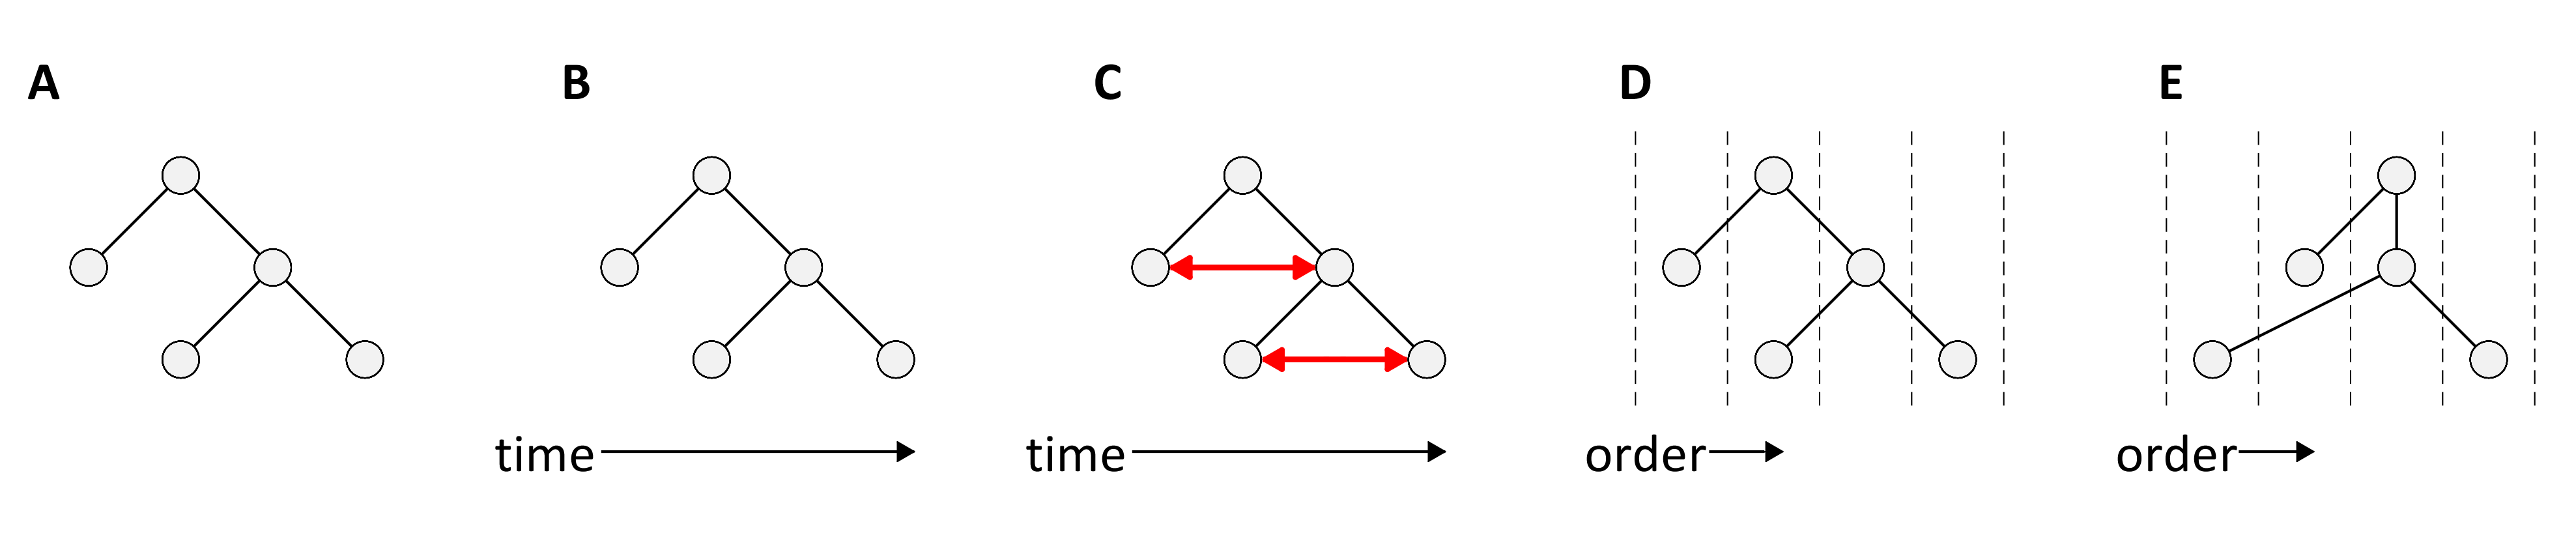
\includegraphics[width=\textwidth]{figures/Tilsen-img1.png}
\caption{\missingcaption}
\label{fig:}
\end{figure}
 

  If the time dimension in (B) made sense, we could draw inferences from horizontal distances between units: two horizontally equidistant units as in (C) would be equidistant in time. This is never the intent of such representations, and in many uses, the horizontal dimension does not even represent order, i.e. discretized time. Hence (D) is equivalent to (E). Because syntactic representations lack an explicit conception of time, a separate mechanism, “linearization”, is needed to map words to a linear order.  However, a close analysis of linearization reveals that temporal information is indeed present in syntactic structures, hidden in connection patterns and orientation. Syntactic structures \textit{do} provide temporal information, but do so indirectly.

  In the oscillators and energy levels framework (henceforth o/el), we bring time into the picture, but not by imposing a temporal dimension on a space which contains objects. Instead, the o/el picture evokes two conceptions of time, both of which differ from our usual, linear conception. One of these is periodic time. Periodic time is useful because we hypothesize that a fundamental property of syntactic and conceptual systems is a capability to transiently oscillate. The transience implies that the oscillation occurs for a brief period of time, as shown in (A): 

  
\begin{figure}
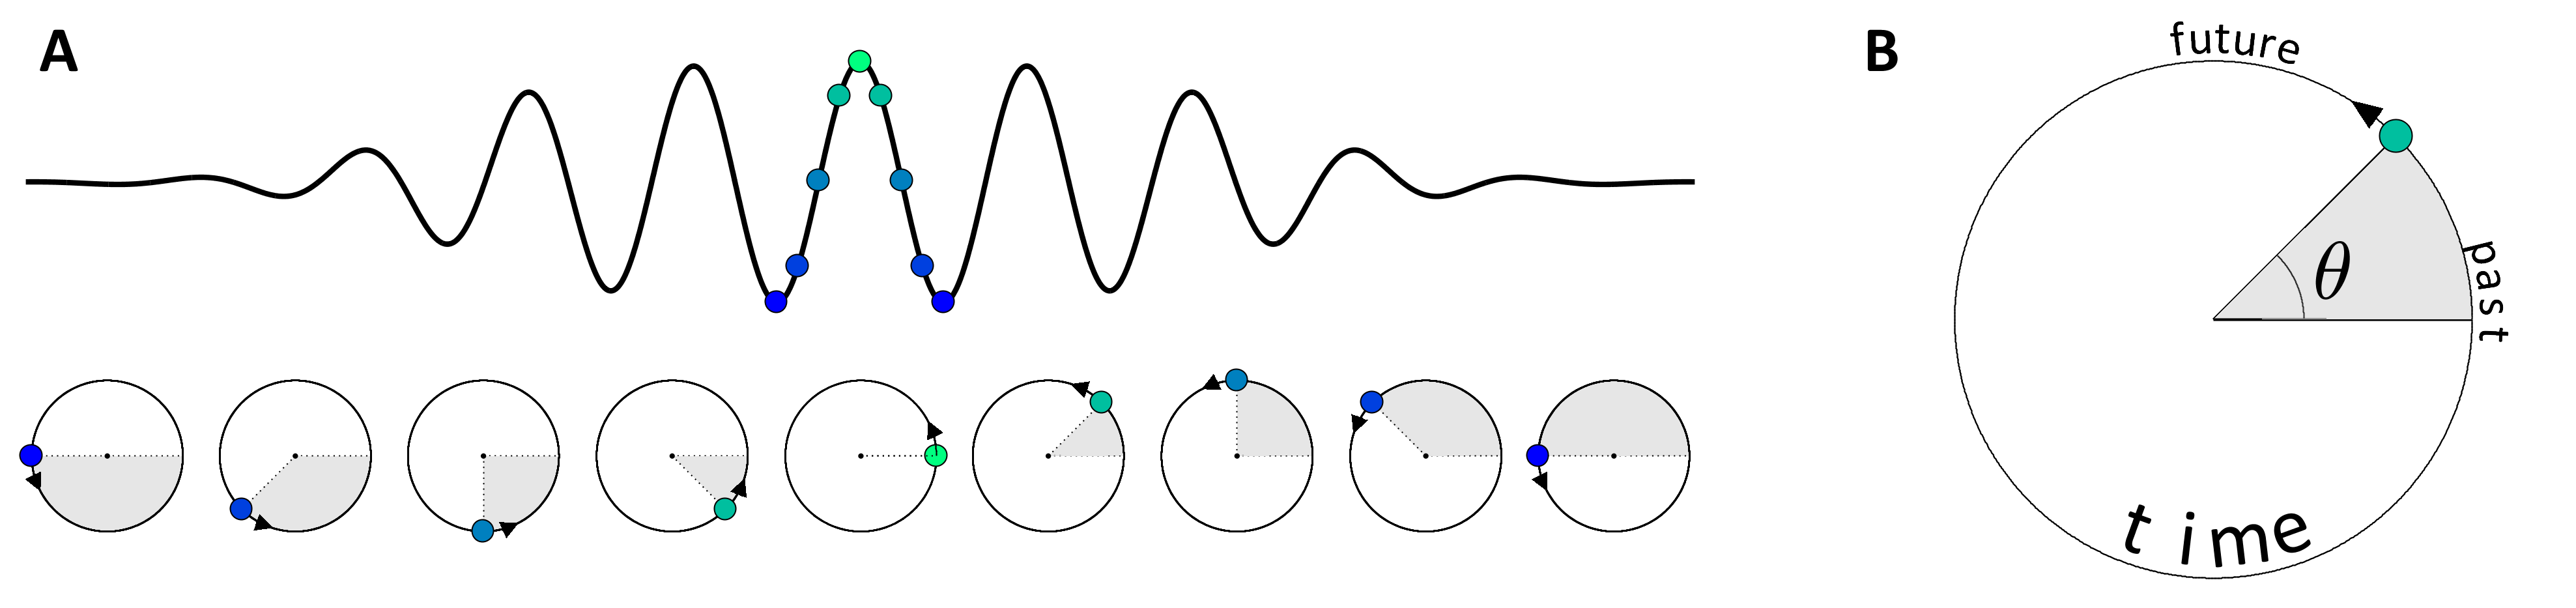
\includegraphics[width=\textwidth]{figures/Tilsen-img2.png}
\caption{\missingcaption}
\label{fig:}
\end{figure}
 

  For an oscillating system, we can picture a circular axis of time as in (B). A specific time is a particular \textit{phase angle}, θ, defined relative to a reference phase angle. The choices of the reference phase and angular units are arbitrary: 0°, 0 radians, or 3:00 are just as useful as 90°, π/2 radians, or 12:00. Phase angle is periodic by definition, so a phase of 360° maps to 0°. Though we are familiar with the angular mapping of time because of circular clocks, some aspects of this conception do not gel with our commonsense intuitions. For instance, periodic time has local notions of past and future, but no global or absolute past or future. There is also an implied frequency parameter, which describes how periodic time maps to linear time: the period of an oscillation (T) is the reciprocal of the frequency (\textit{f}).

  Periodic time provides a useful description of a temporal relation between a pair of oscillating systems: \textit{relative phase}, φ. Relative phase is the difference between the phase angles of two systems, as illustrated below. For a pair of systems \textit{i} and \textit{j}, φ\textit{\textsubscript{ij}}\textsubscript{} = θ\textit{\textsubscript{i}} - θ\textit{\textsubscript{j}}. Patterns of φ are of fundamental importance in the o/el framework: a central proposal is that transiently stable φ configurations give rise to the experience of relational meaning.  

  
\begin{figure}
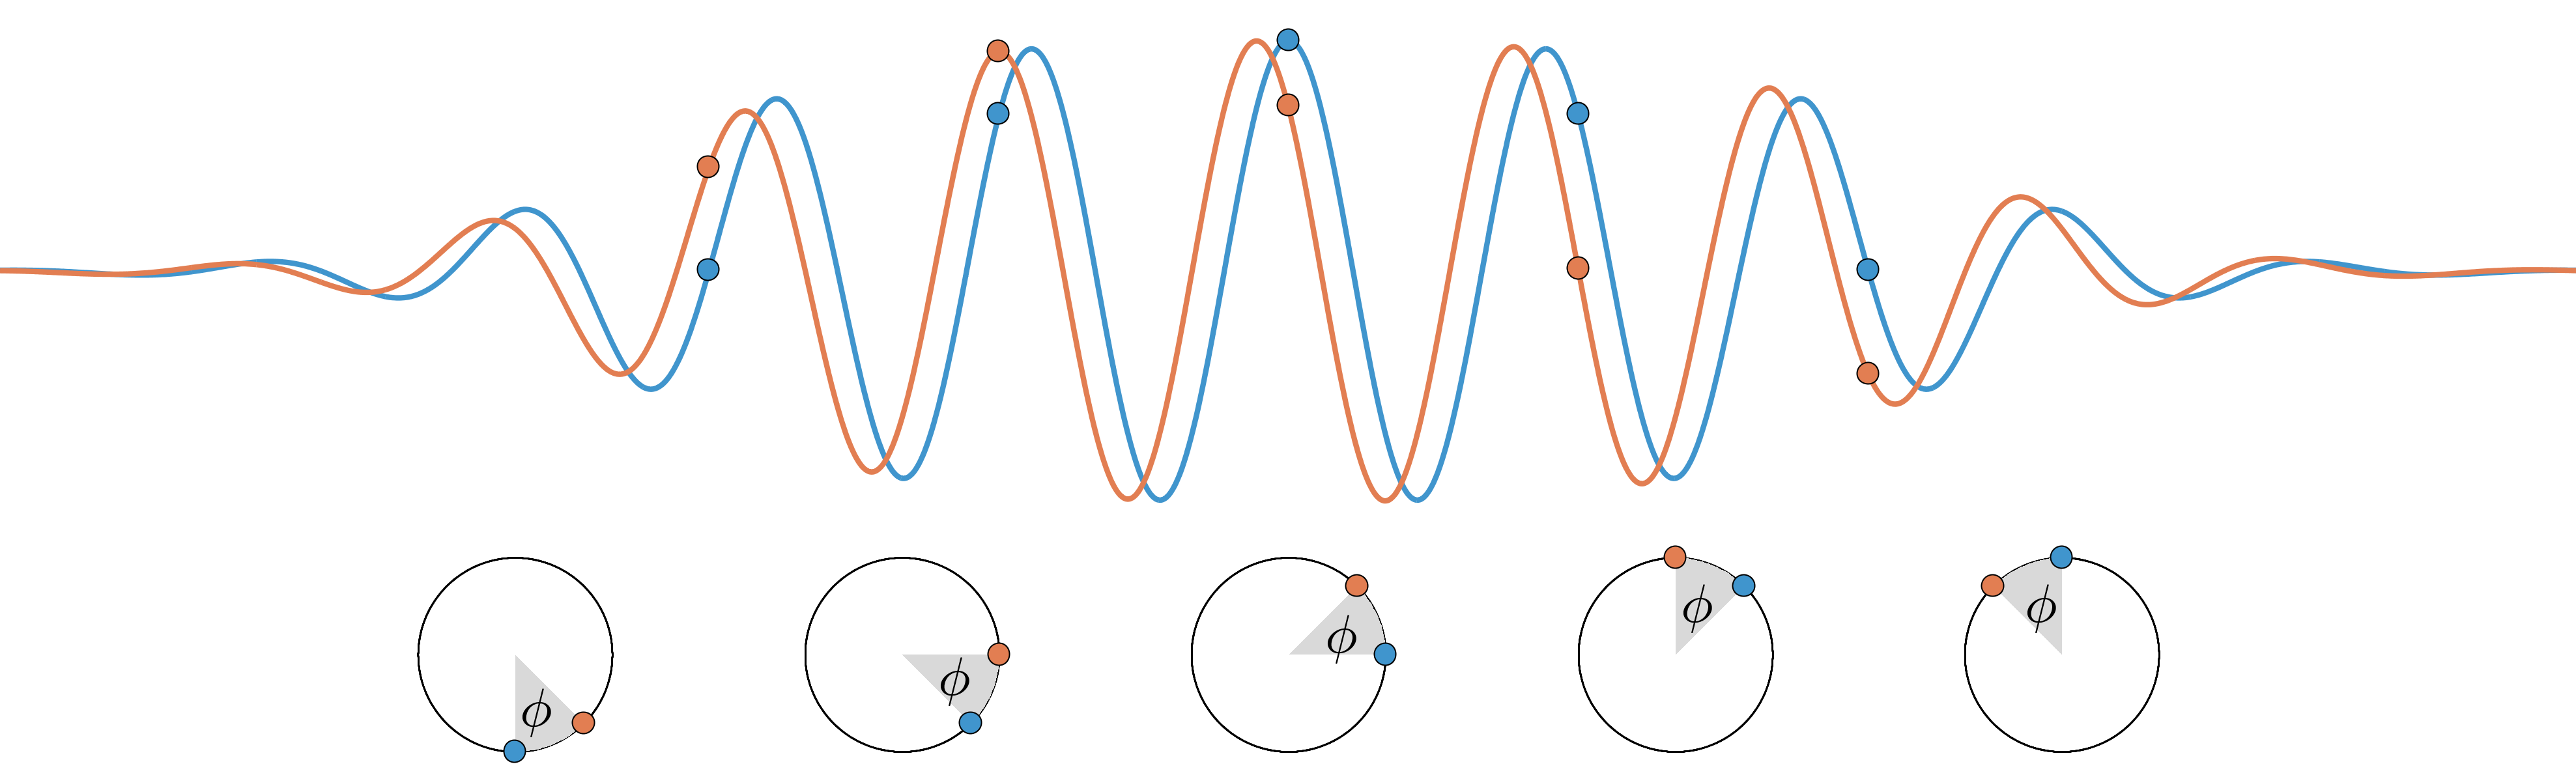
\includegraphics[width=\textwidth]{figures/Tilsen-img3.png}
\caption{\missingcaption}
\label{fig:}
\end{figure}
 

  The other conception of time in the o/el framework is discontinuous, piecewise-linear time. Why is this useful? Lets imagine a system in which some quantity normally changes slowly or stays constant, but certain processes occasionally cause the quantity to change very abruptly. As shown below, a continuous but highly nonlinear change of this sort can be approximated as a discontinuity when viewed on a larger scale.

  
\begin{figure}
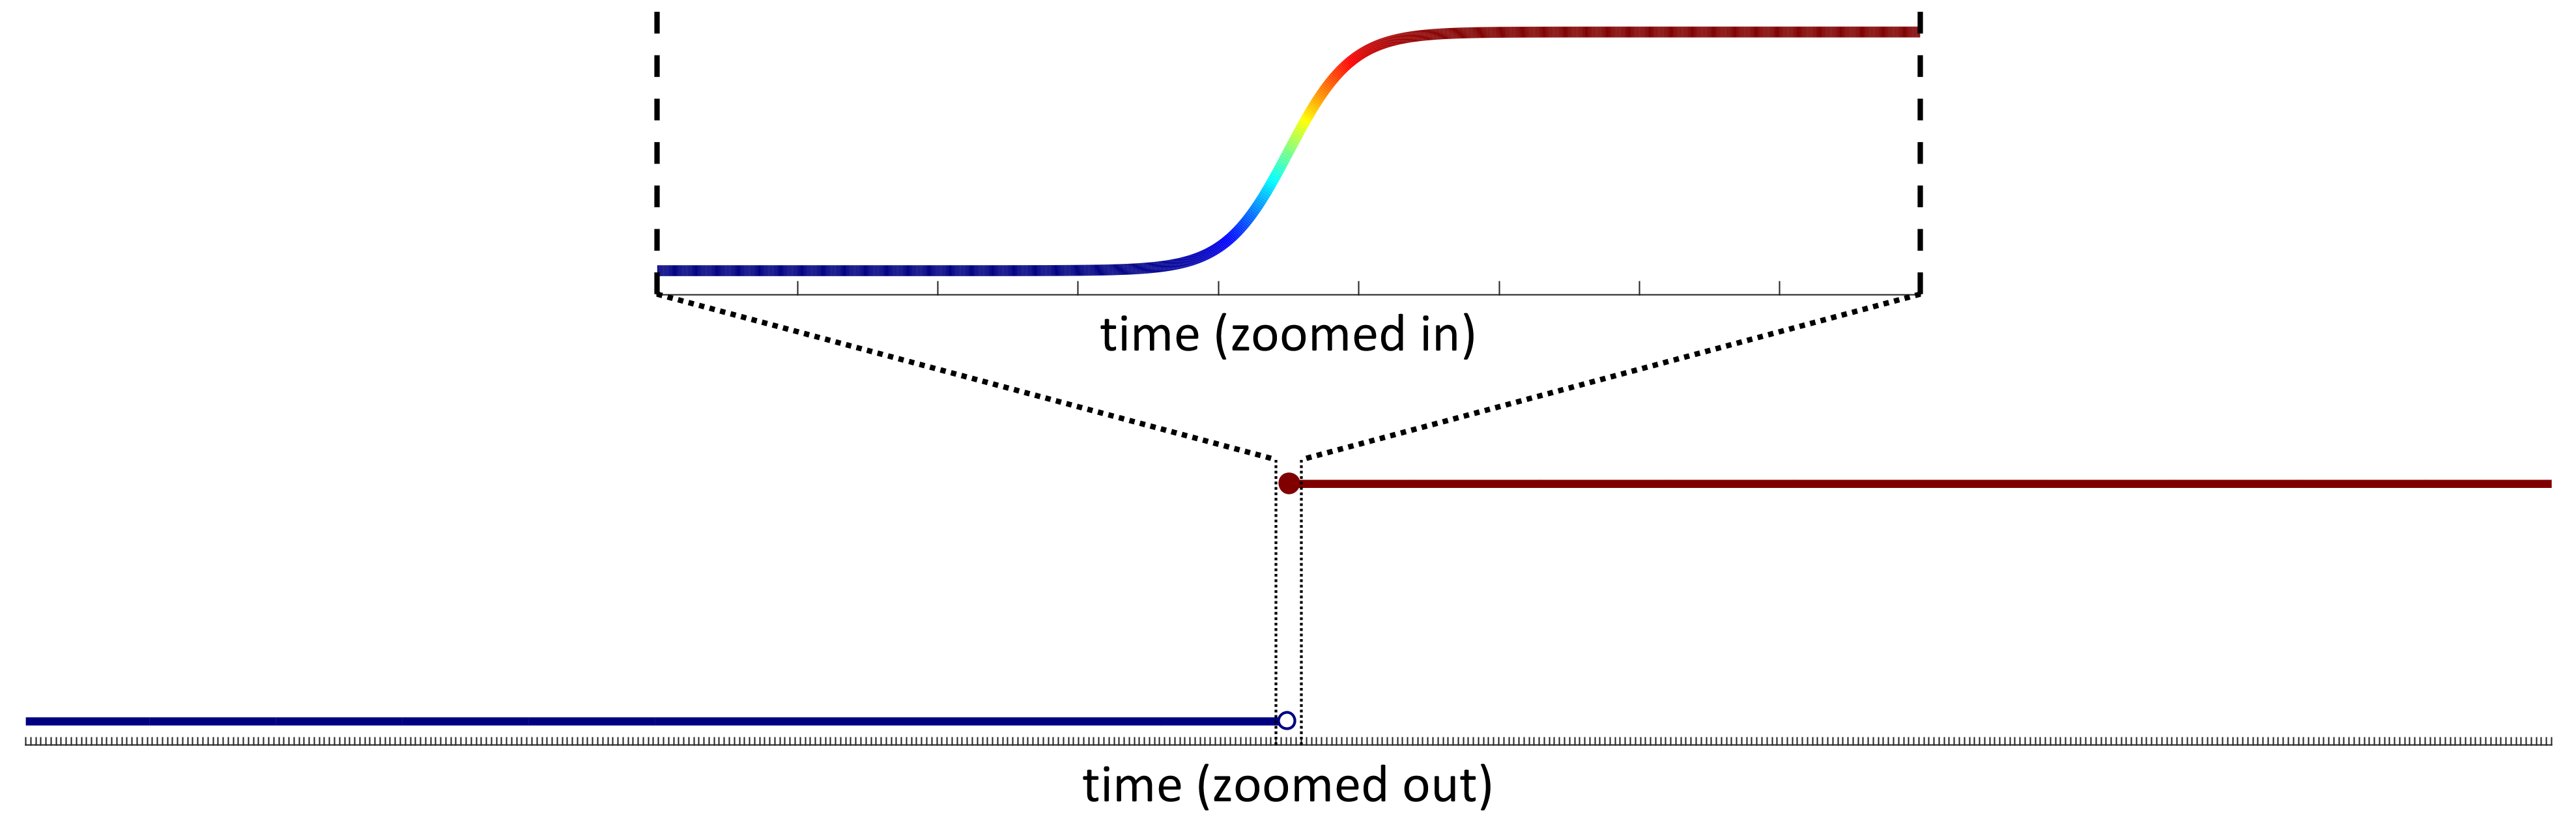
\includegraphics[width=\textwidth]{figures/Tilsen-img4.png}
\caption{\missingcaption}
\label{fig:}
\end{figure}
 

  Temporal discontinuities are useful because the timescale of processes which govern the ordering of motor behaviors is smaller than the timescale on which relational meaning experiences (i.e. φ patterns) remain stable. Moreover, we hypothesize a mechanism for rapid organization and reorganization of syntactic systems into hierarchically related levels of excitation, as shown below.

  
\begin{figure}
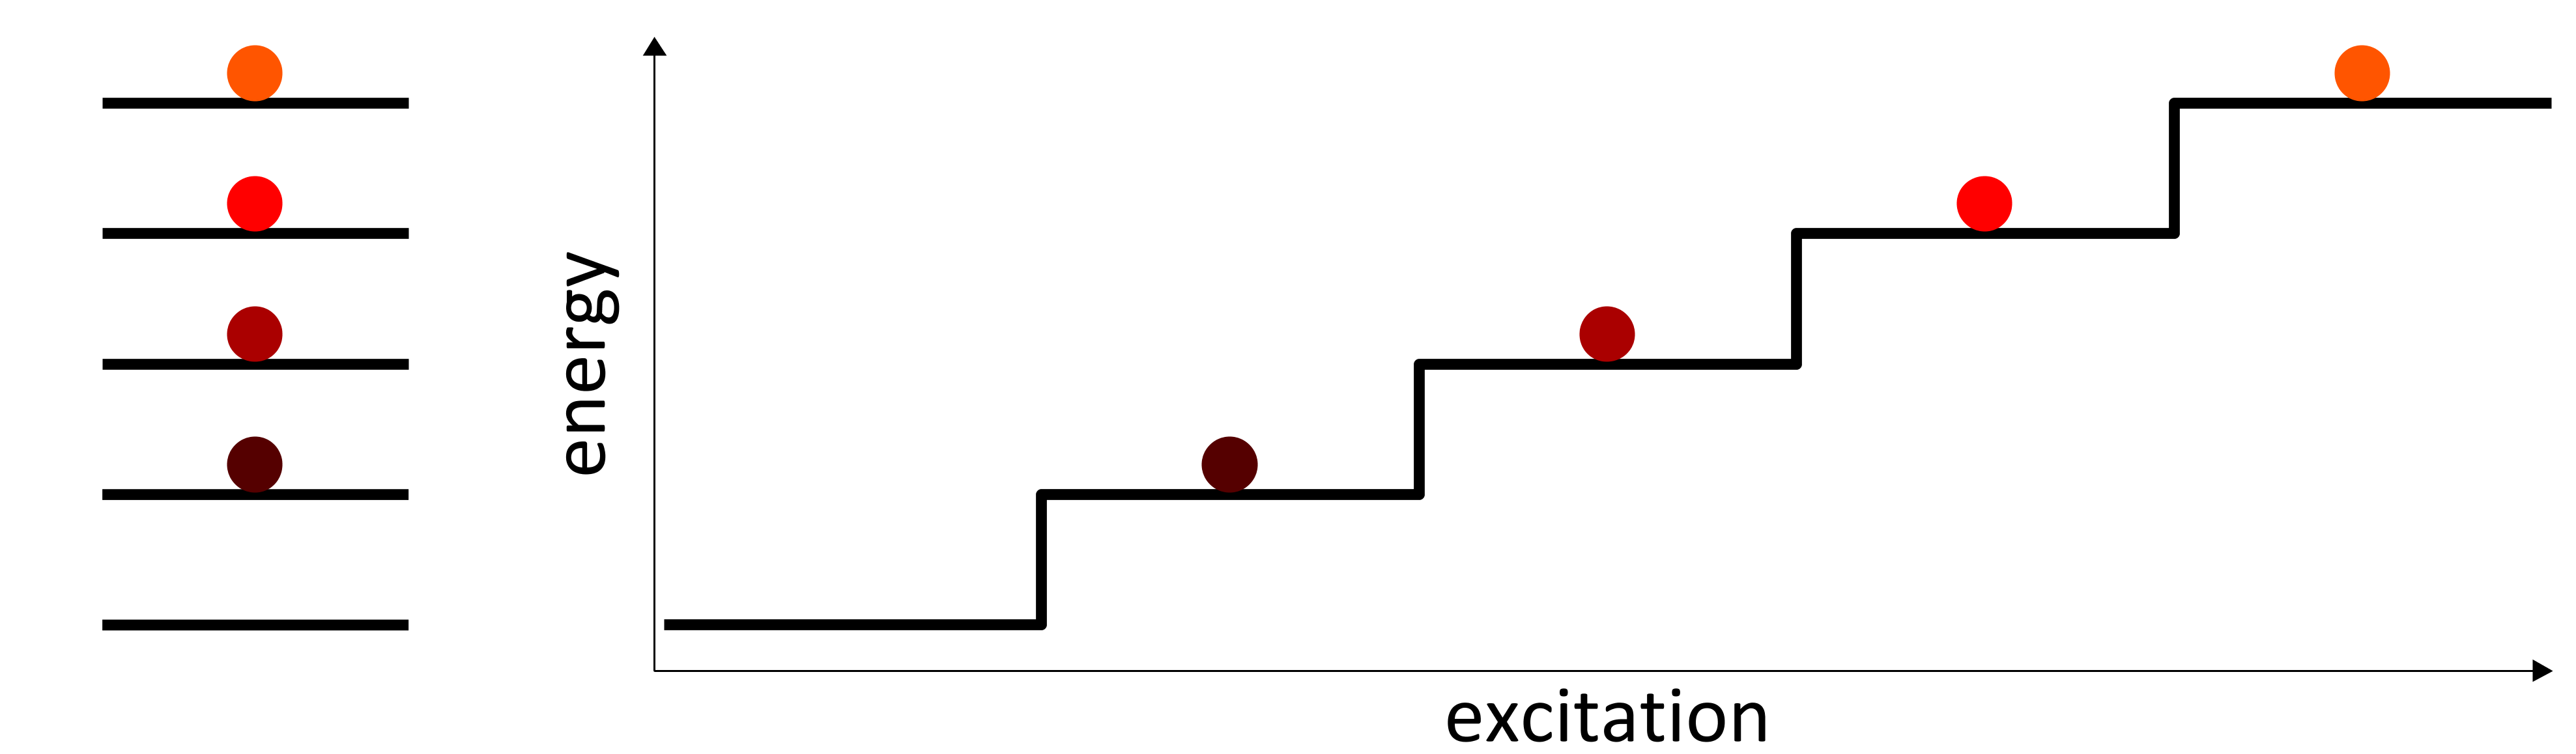
\includegraphics[width=\textwidth]{figures/Tilsen-img5.png}
\caption{\missingcaption}
\label{fig:}
\end{figure}
 

  The production mechanism operates via iterated reorganization of the excitation hierarchy, as illustrated in the {\figurebelow}. In epoch (e\textsubscript{1}), the most highly excited system is selected and corresponding motor actions are performed. Subsequently, the selected system is demoted while other systems are promoted—a reorganization occurs, resulting in a new stable epoch, (e\textsubscript{2}). As shown below, the reorganization process is iterated, resulting in the production of a sequence of words.

  
\begin{figure}
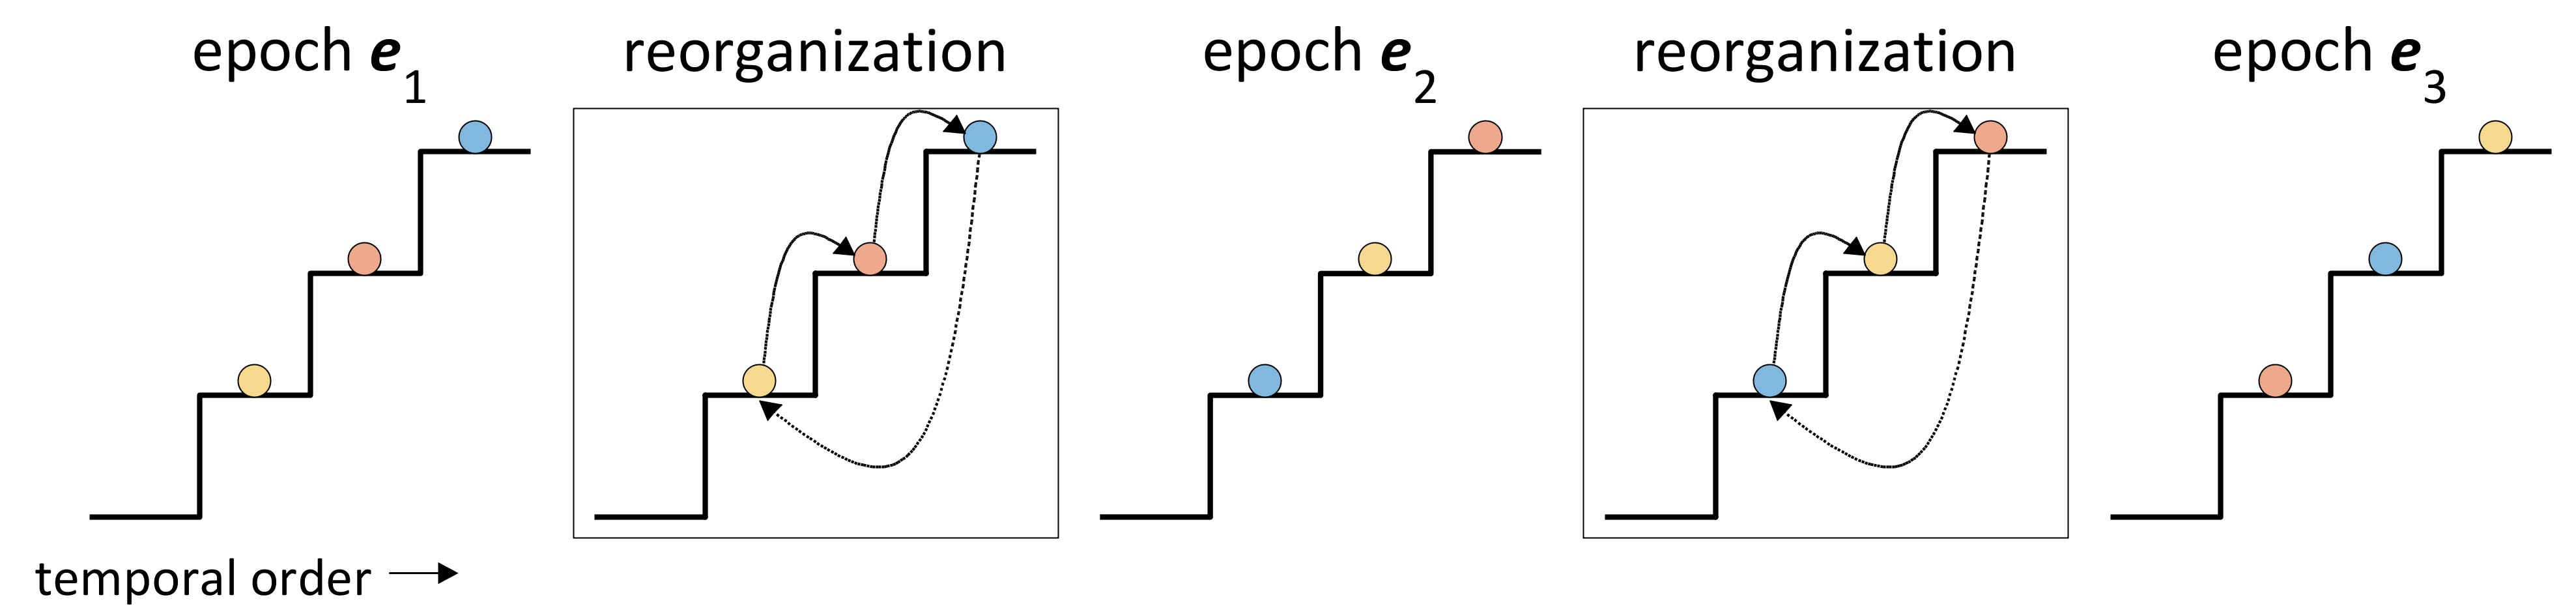
\includegraphics[width=\textwidth]{figures/Tilsen-img6.png}
\caption{\missingcaption}
\label{fig:}
\end{figure}
 

  Instead of obscuring time, o/el representations are designed to facilitate reasoning about temporal patterns. The blend of temporal conceptions which is evoked by the o/el framework highlights a tension between continuity and discontinuity that underlies nearly all of our reasoning about language. Bringing this tension to the foreground helps us better understand a wide variety of syntactic phenomena in the production and interpretation of language.

The other big problem with conventional theories is \textit{the problem of multiplicity}. In syntactic trees (and alternative representational schemas), a given type of syntactic object (e.g. N, V, S, VP, etc.) can be present in an arbitrary number of positions in a structure, as below. Conventional frameworks impose no limit on the number of instantiations of a given type of object. No adverse consequences of multiplicity are expected, even when multiplicitous objects are associated with the same word, e.g. the verb \textit{knows} in the utterance \textit{Al knows that Bo knows that Cam knows…}  

  
\begin{figure}
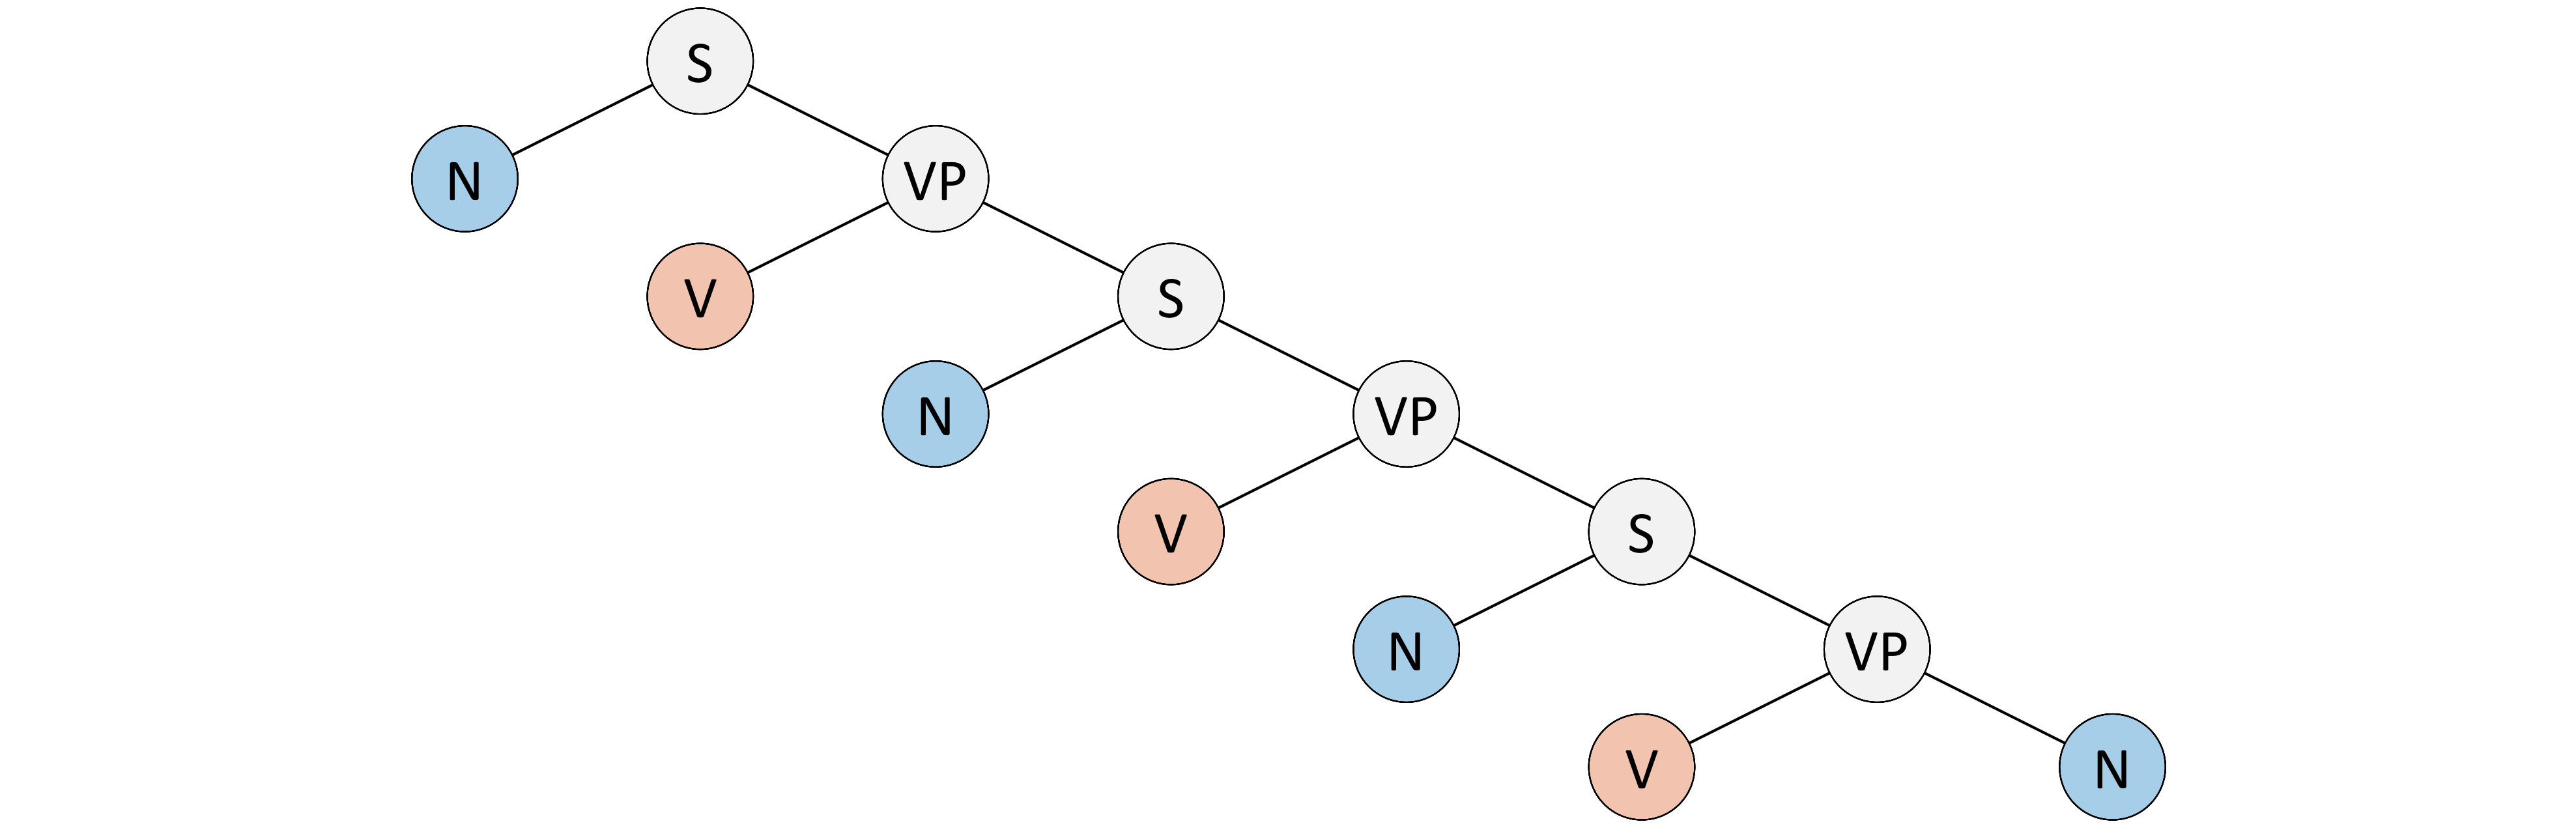
\includegraphics[width=\textwidth]{figures/Tilsen-img7.png}
\caption{\missingcaption}
\label{fig:}
\end{figure}
 

  The acceptance of multiplicity is so deeply ingrained (perhaps due to written language) that most theories fail to recognize the problem. The issue is that if we believe syntactic patterns can be understood in relation to macroscopic brain states, then we must accept a finite capacity for distinct states. Multiplicitous conceptions of structure provide no intrinsic mechanisms for understanding the nature of limitations on this capacity.

  Any syntactic theory must either ignore or resolve the multiplicity problem. We should prefer a theory in which the resolution derives from the same conceptual model that provides a basis for understanding linguistic phenomena generally—a \textit{comprehensive} theory. Many current approaches fall short of this because their solution is to distinguish between competence and performance, in effect stipulating that mechanisms of syntactic organization can be isolated from other cognitive mechanisms. The o/el framework addresses the multiplicity problem by developing a mechanism for systems (construed microscopically as neural populations) to differentiate into subsystems (overlapping subpopulations). Because differentiated subsystems interfere with one another, differentiation leads to interference that can destabilize those systems. Stability has important consequences for what speakers produce and what is coherent for an interpreter.

  This book is organized into several chapters. The first chapter, \textsc{Overview of the oscillators/energy levels framework}, introduces the basic microscopic and macroscopic conceptual models which provide a basis for reasoning about syntactic phenomena. \textsc{Deconstructing syntactic theory} discusses how conventional syntactic theories are based on a small set of fundamental metaphors and image schemas, and contrasts these with the metaphors used in the oscillators/energy levels framework. \textsc{Reconstructing syntactic theory} provides a detailed presentation of the o/el model. The focus is on phrase structure, but some morphosyntactic and morphophonological phenomena are covered as well. Most importantly, the concept of interference is developed in detail, and this motivates analyses in subsequent chapters. \textsc{Infinity and recursion} argues that viewing language as a discrete infinity generated by recursive merge operations is misguided. \textsc{Grammaticality intuitions} argues for reconceptualizing grammaticality intuitions as the result of an experience of the coherence of a system state trajectory; common neurophysiological patterns are interpreted in relation to coherence. \textsc{Syntactic phenomena} applies the o/el framework to three phenomena: ellipsis, anaphora, and movement islands. Finally, \textsc{The physical linguistics program} describes the philosophical underpinnings of the approach taken in this book, and sets the stage for future research.

  There is a small amount of mathematical formalization in this book, which will be of varying degrees of difficulty for readers, depending on their familiarity with dynamical systems. In most of the cases where equations are presented, I have provided illustrations which facilitate a visual conceptualization. It is my belief that a sufficient understanding of the mathematical concepts can be obtained from the visual/geometric illustrations alone, without a need for interpreting the symbolic math. The equations are merely a convenient shortcut for describing geometric patterns. For readers who would like to become more familiar with the relevant math, including how it can be related to behavior, I would recommend two introductory texts: \textit{Dynamic Patterns: The self-organization of brain and behavior}, by J. A. Scott Kelso \citep{Kelso1997}, and \textit{Nonlinear dynamics and chaos}, by Steven H. Strogatz \citep{Strogatz2018}. Familiarity with these texts is a not a prerequisite for understanding the current approach, but will undoubtedly enrich the interpretation of the approach developed here. For more technical texts which address dynamics from biological, neurological, and physical perspectives, it is suggested that the reader consult \textit{The Geometry of Biological Time} by Arthur T. Winfree \citep{Winfree2001}, \textit{Dynamical Systems in Neuroscience} by Eugene M. Izhikevich \citep{Izhikevich2007}, and \textit{Advanced Synergetics: Instability Hierarchies of Self-Organizing Systems and Devices} by Hermann Haken \citep{Haken1983a}.

  Some portions of this book present critiques of “conventional” syntactic theories, especially in the second chapter, \textsc{Deconstructing syntactic theory,} and in the fourth chapter, \textsc{Infinity and recursion}. These critiques are related to the problems of atemporality and multiplicity discussed above. A warning is necessary regarding the targets of the critiques. There are numerous syntactic theories/frameworks: 
  Minimalism \citep{Chomsky1995}, 
  Categorial Grammars (\citealt{Steedman1993,Wood2014}), 
  Tree Adjunction Grammars \citep{Joshi1987}, 
  Lexical Functional Grammar \citep{BresnanKaplan1982}, 
  Dependency Grammar (\citealt{Hudson1977,Tesnière2018}), 
  Generalized Phrase Structure Grammar 
  \citep{GazdarEtAl1985},
  Functional Grammar \citep{Dik1981}, 
  Role and reference grammar \citep{VanValinJr2014},
  Construction Grammar \citep{Goldberg1995}, 
  Radical Construction Grammar \citep{Croft2001}, 
  Sign-Based Construction Grammar \citep{Sag2012}, 
  Semiotic Grammar \citep{Mcgregor1997}, 
  Cognitive Grammar \citep{Langacker2008}, and others. It is beyond the scope this book—or\todo{check dashes across document} perhaps any single book, for that matter—to critique all of these frameworks.

Rather than being general, the critiques herein specifically target Minimalism and its precursors, Transformational Grammar \citep{Chomsky1965} and Government and Binding Theory \citep{Chomsky1982}, which fall under the label of generative grammar. These frameworks are the ones that we subsequently refer to as “conventional theories,” although this label is not intended to imply that these particular frameworks are more standard or widely accepted than others. Instead, “conventional” implicates a set of foundational metaphors which \textit{by convention} constitute a basis for reasoning about syntactic phenomena. However, by narrowing the target in this way, the question is raised of whether the critiques apply to other theories/frameworks. Certainly not all aspects of the critiques necessarily apply to all extant theories. It is left as an exercise for readers—many of whom are better versed in some of the particular approaches listed above—to consider whether the atemporality and multiplicity problems (and the collections of critiques they encompass) apply to a given syntactic framework. Nonetheless, it is my impression as an outsider that the foundational metaphors discussed herein are very general, and I bring attention to the metaphors in order to provoke a re-examination of their usefulness.

\chapter{Overview of the oscillators/energy levels framework}
The o/el framework and conventional frameworks offer very different conceptualizations of “syntax”. In conventional approaches, a syntax “module” builds “structures” of “objects” which map both to speech motor output and to a meaning representation. This modular approach separates syntax from the phenomena that are most directly important for communication: movements/sensory experiences (a.k.a. the sensorimotor interface, phonological form), and meaning experiences (a.k.a. the conceptual-intentional interface, logical form). The modular interface view encourages us to see syntax as independent from meaning and independent from movement/sensation. We should reject this way of thinking. Syntax should not be understood as a module, but as a generic term for mechanisms which organize meaning and sensorimotor experience. Experiences are highly ordered states, and syntax is a mechanism for creating order. 

  The o/el framework rejects modules and instead embraces the notion of a \textit{system}. A system is a portion of the universe associated with some partially predictable mapping from input information to output information. In the o/el conception there are many systems, of two fundamental types: concept systems and syntactic systems. Unlike the weak, unidirectional interfaces of modules, o/el systems may have strong, bidirectional interactions. Even more importantly, o/el systems do not operate on structures of “objects”. Instead, concept systems and syntactic systems have states and exert forces on one another. Below we develop a detailed picture of these systems and their interactions. 

  An important way in which the current approach differs from conventional ones is that we attempt to motivate the framework with inferences based on knowledge of neural population dynamics. The o/el framework is derived from a microscopic conceptualization in which population coding and interpopulation connectivity play major roles in determining behavioral patterns. There are many ways in which our derivation of a macroscopic analysis relies on incomplete information and unsubstantiated assumptions regarding the microscale; I accept the possibility that invalidation of the microscale assumptions may compromise the framework.

\section{Concept systems}

How do complex patterns of thought arise in the brain? For example, consider the sentence \textit{Al drinks coffee}. In the conventional metaphor, a phrase is a “structure of objects” that arises from the merger of smaller objects. These objects—words and phrases, i.e. “linguistic units”—are also the sort of objects that can be “containers”. Thus words contain meaning and phrases contain words. Connected object representations as below use vertical orientation and connection schemas to encode these containment relations:

  
\begin{figure}
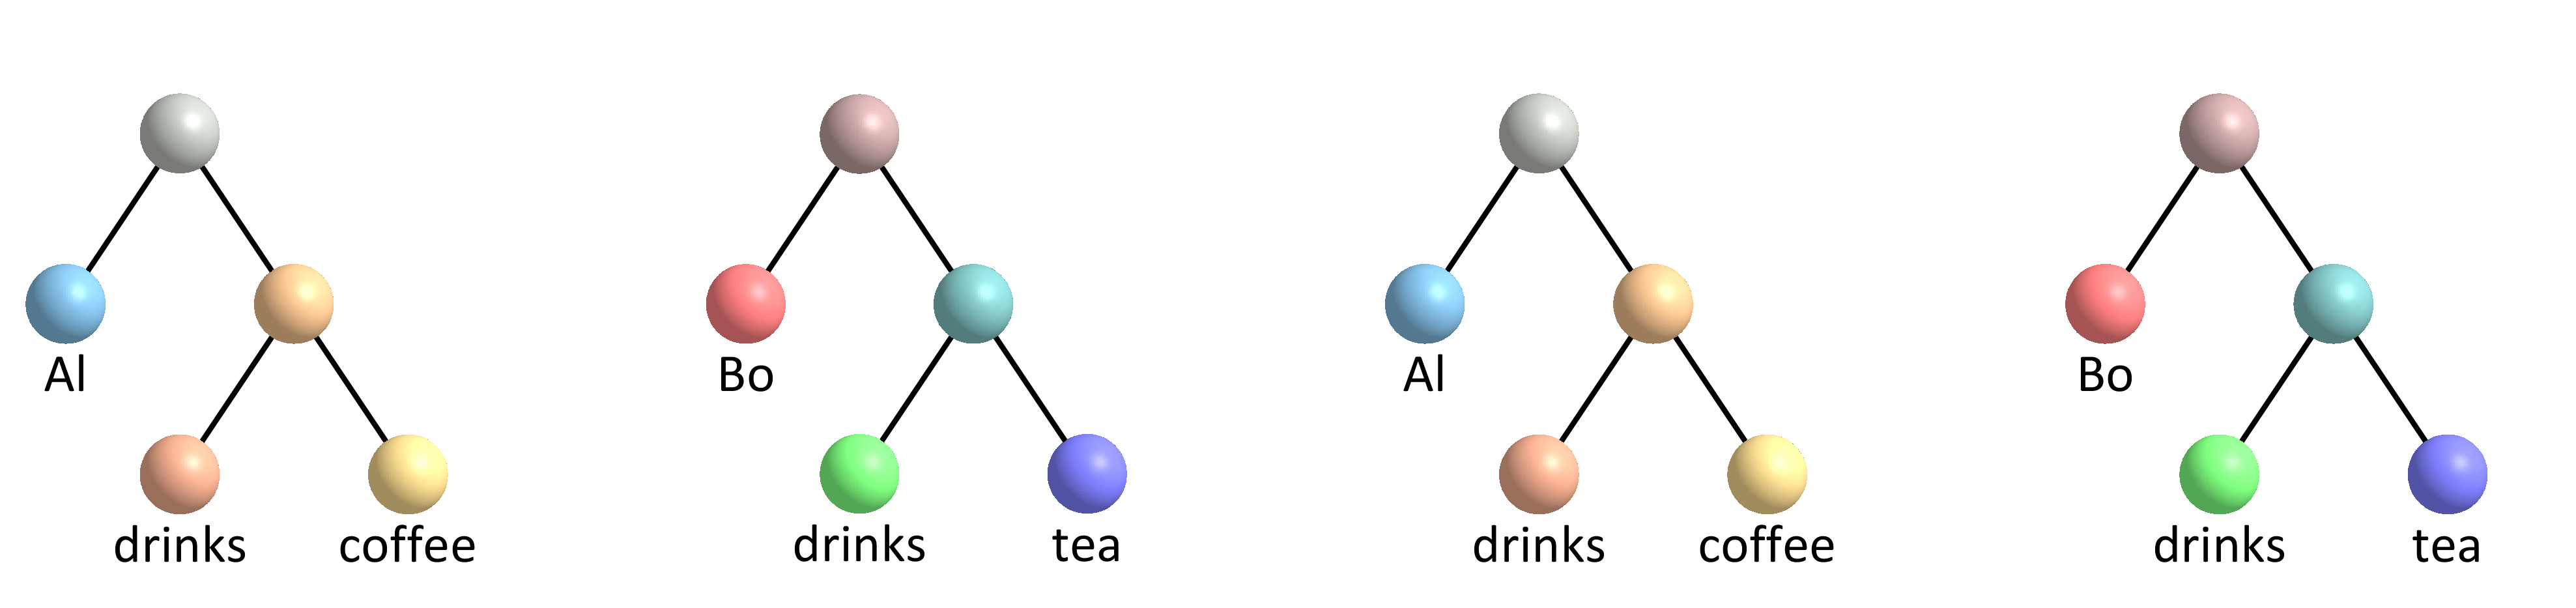
\includegraphics[width=\textwidth]{figures/Tilsen-img8.png}
\caption{\missingcaption}
\label{fig:}
\end{figure}
 

  Are schemas of this sort useful? Imagine the following scenario, in which you engage two thought patterns in succession. First, you engage the pattern \textit{Al drinks coffee}. Next, you engage an alternative pattern, \textit{Bo drinks tea}. Then, you return your attention to \textit{Al drinks coffee.} Then, back again to \textit{Bo drinks tea}. And so on… What would we expect to observe in the brain in this scenario? 

  The connected objects schema is not well suited for addressing this question. Because these sentences are conceptualized as structures of objects, we can ask: “where do the objects come from?”, “how do they become connected or combined?”, and “what happens to them when we switch to a different pattern?” Do the objects get destroyed? Do they move somewhere? Do they vanish, are they hidden? Do the objects ever change over time? Where are these objects located in space? Etc.

  The essence of the problem is that conventional approaches force us to think of linguistic units \textit{as objects}. To construct abstract understandings of phenomena, we often use the \textsc{abstractions-}\textsc{are}\textsc{{}-objects} metaphor (e.g. \textit{put your feelings aside}, \textit{tear an argument into pieces}, \textit{build a new life}, etc.). But regardless of how familiar it is and how intuitive it seems, the \textsc{units}\textsc{{}-are-}\textsc{objects} metaphor is not necessarily a useful conceptualization of language. 

  In the o/el framework, linguistic units are \textit{not} objects. They are not the sorts of things that contain meaning, and are not the sorts of things that can be connected. They do not occupy space, they do not have orientational relations. The o/el framework rejects all entailments of the \textsc{units}\textsc{{}-are-}\textsc{objects} metaphor. Instead, we adopt an alternative in which meanings are experiences, experiences are trajectories of system states in a state space, and various forces influences those trajectories. Our task then becomes construction of a state space, analysis of state trajectories, and determination of forces. Because meaning experiences are trajectories, meanings are inherently temporal. 

\subsection{Concept-specific populations of neurons}

To develop an intuition for the \textsc{meanings}\textsc{{}-are-}\textsc{trajectories} metaphor we consider a simple utterance, \textit{Al drinks coffee.} We pose the following question: \textit{physically}, in space and in time, what happens when a speaker produces this utterance? Lets suppose that in some brief period of time preceding the utterance, in the brain of the speaker, there is a population of excitatory cortical neurons which in a statistical sense\footnote{To assess this empirically, we would want high-spatial and temporal resolution of electrochemical gradients and synaptic connectivities, along with information regarding movements and acoustic signals. Whether this can be accomplished with current technology is beside the point: we can imagine associating populations of neurons with concepts in this way. Note that we require no assumptions about the uniqueness or overlap of the populations at this point. The idea that spiking in distributed populations of neurons (or assemblies, ensembles, etc.) may correspond to things like concepts or words is a fairly old one; see for example (\citealt{Abeles2012,Braitenberg1978,Hebb1949}; Pulvermüller, 1999)} is associated with concepts that contribute to the relevant experience of meaning. For exposition, lets identify those concepts as [Al], [drinks], and [coffee]. Furthermore, suppose that we can differentiate the population into an [Al] subpopulation, a [drinks] subpopulation, and a [coffee] subpopulation. Thus each concept is associated with a population of many neurons. No strong assumptions are necessary regarding the temporal permanence, spatial distributions, sizes, or independence of these concept populations.

  
\begin{figure}
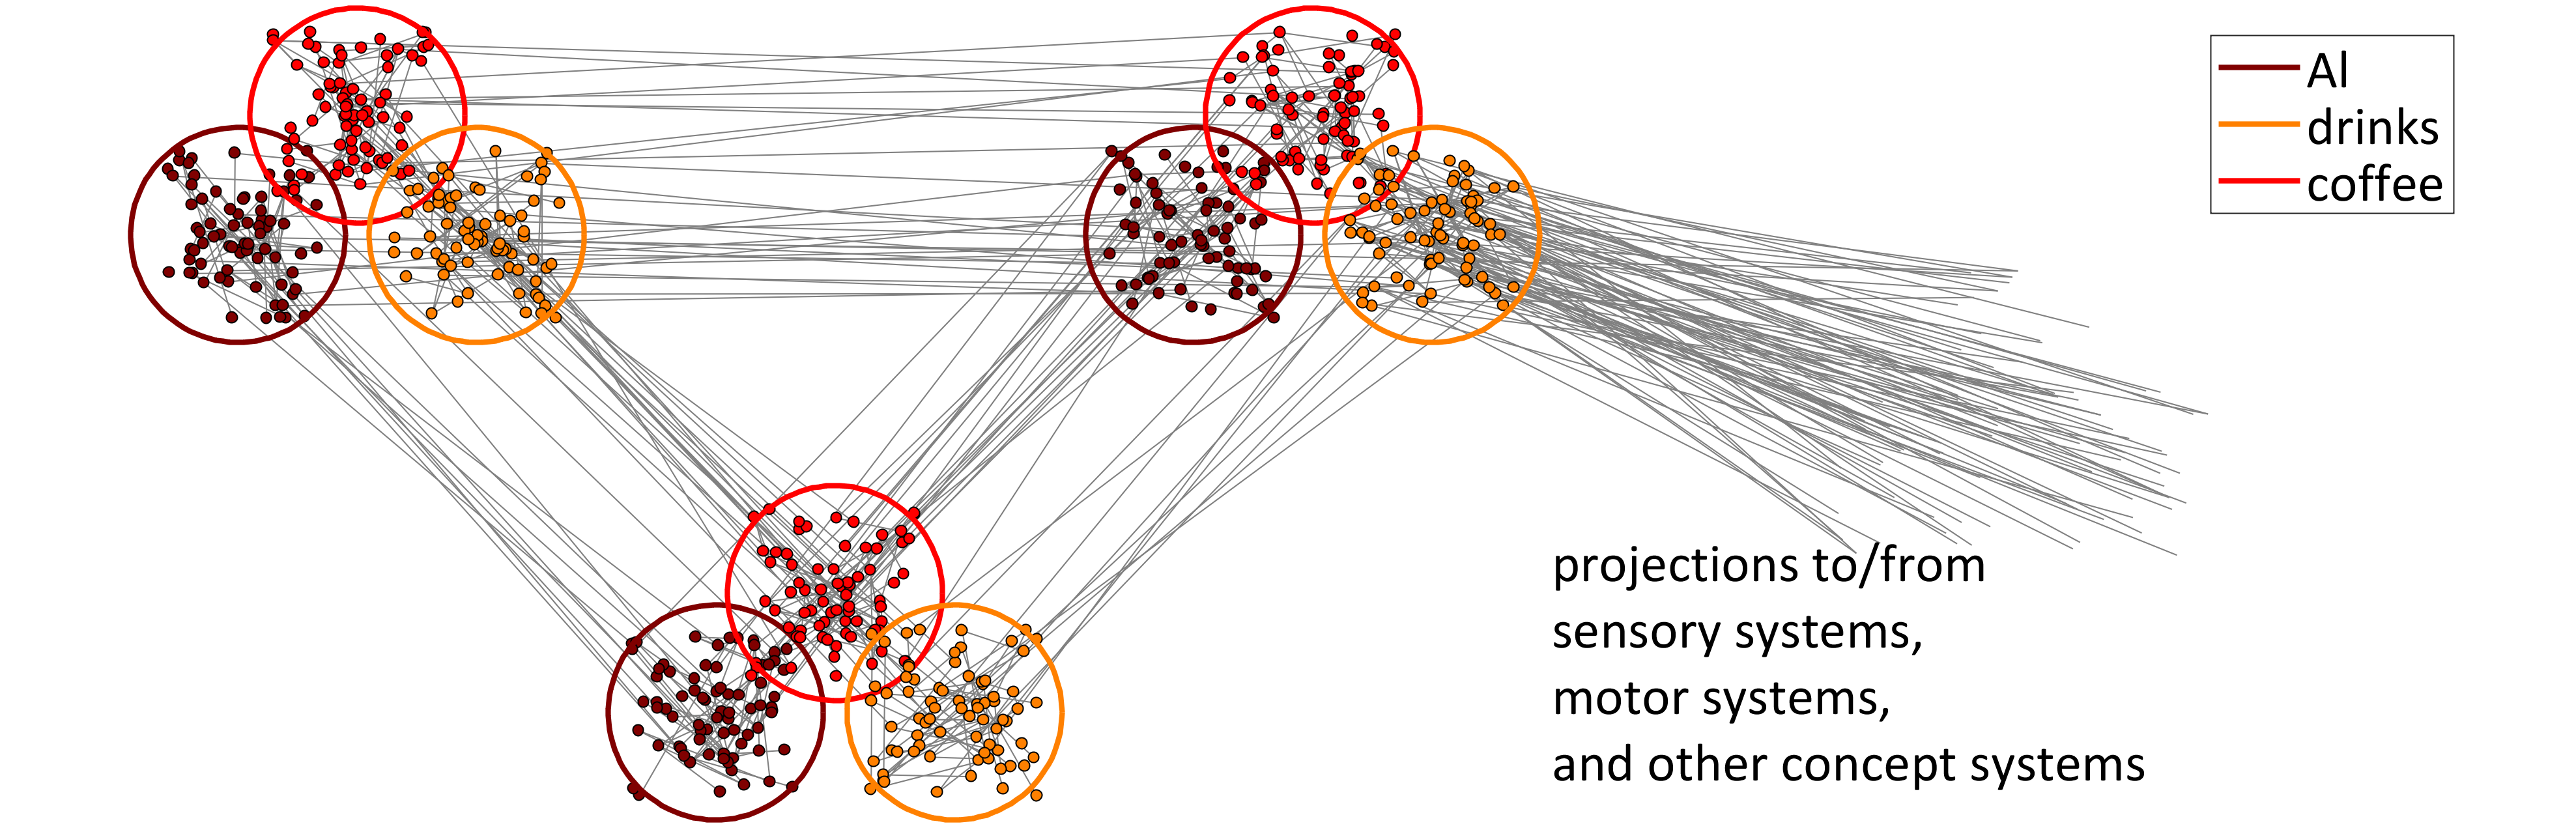
\includegraphics[width=\textwidth]{figures/Tilsen-img9.png}
\caption{\missingcaption}
\label{fig:}
\end{figure}
 

  The picture above shows populations that are \textit{distributed}: concept populations are associated with neurons in multiple regions of the brain, rather than just one region. Moreover, the “meanings” of concepts are qualia which we assume to be determined by the structure of projections to and from sensory systems, motor systems, and other concept populations. For example, our experience of \textsc{coffeeness} is a consequence of patterns of projections to and from the peripheral sensory systems which provide us information regarding taste, odor, appearance, temperature, etc. of coffee, as well as the motor systems which we use to pour coffee, drink it, brew it, and also other concepts which relate to \textit{coffee}: beans, cups, caffeine, etc. There is no essential meaning of \textit{coffee} because the pattern of projections varies over time within an individual and varies in space, i.e. between individuals.
\subsection{{\textbf{Phase transitions to collective oscillation}}}

Before a speaker experiences a meaning associated with [Al], [drink], and [coffee], the neurons of each of these concept populations must undergo a phase transition from an \textit{inactive} regime, in which action potentials are sparse in time and relatively uncorrelated, to an \textit{active} regime, in which action potentials are frequent and highly correlated. We conjecture that integrating action potentials for each population on an appropriate timescale results in an oscillatory spike-rate\footnote{There is plenty of evidence that oscillation plays an important role in the nervous system, and that neural populations exhibit oscillatory patterns of spiking (\citealt{AverbeckEtAl2003,Buzsaki2006,BuzsákiDraguhn2004,CanoltyKnight2010,EngelEtAl2001,Fuster2001,GerstnerKistler2002,Izhikevich2006,Izhikevich2007,IzhikevichEdelman2008,Klimesch1999}). However, because concept populations are hypothetical, the assumption that these populations oscillate is a conjecture.}, as shown below. We conceptualize this phenomenon as the emergence of a macroscopic \textit{collective oscillation} \citep{AcebrónEtAl2005,BreakspearEtAl2010,HongStrogatz2011,Kelso1997,SchonerKelso1988,Strogatz2000,Winfree2001}. The causes of these phase transitions are various, but lets imagine for concreteness that the speaker sees a man named \textit{Al} and a dark liquid falling into his mouth from a cup he holds. We infer that this peripheral sensory information, through a chain of interactions, causes the relevant concept populations to undergo transitions to the collective oscillation regime.


  
\begin{figure}
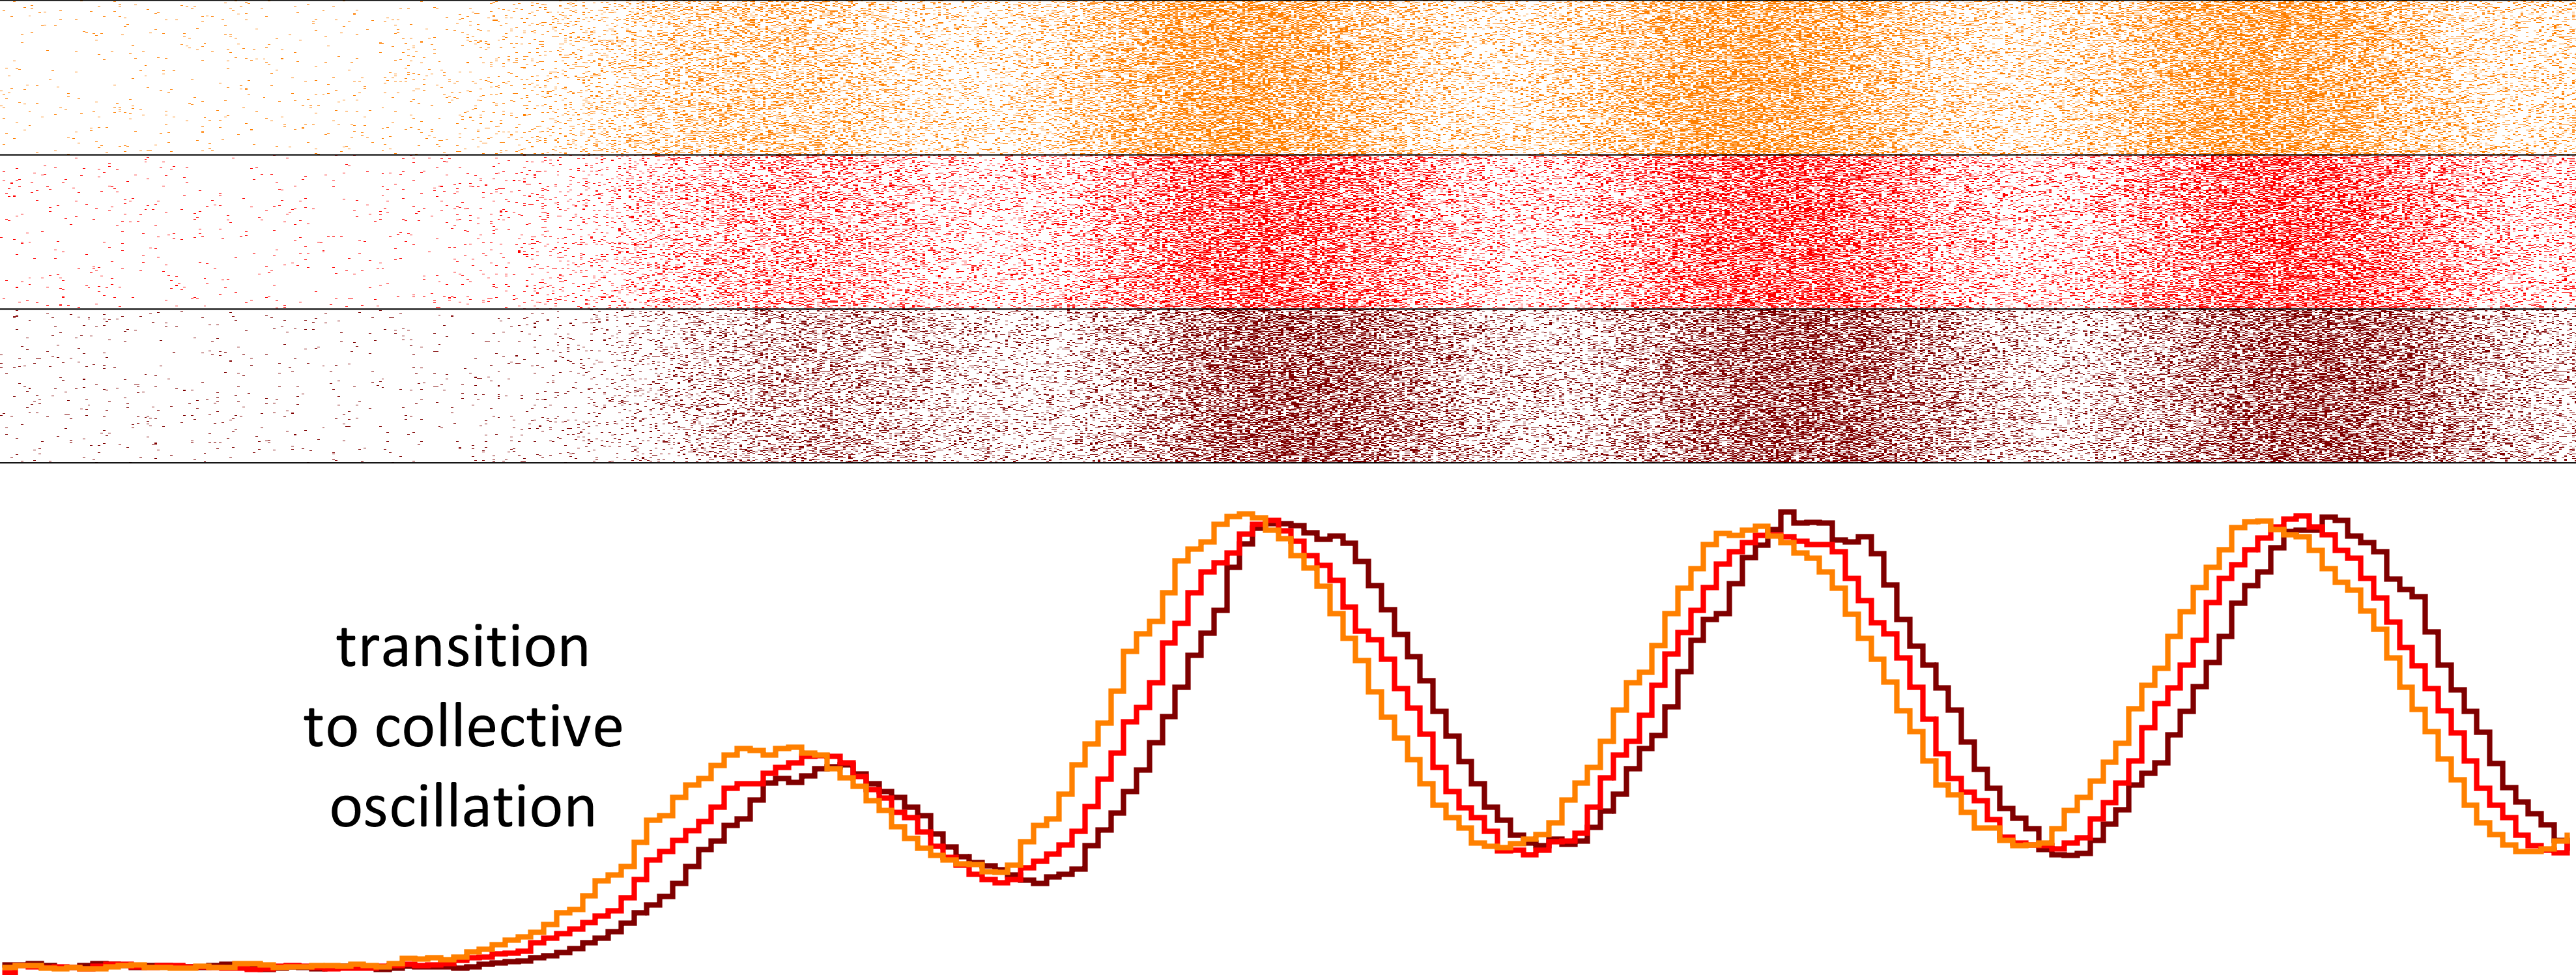
\includegraphics[width=\textwidth]{figures/Tilsen-img10.png}
\caption{\missingcaption}
\label{fig:}
\end{figure}
 

  The transition to collective oscillation is a localized emergence of a state that is highly ordered in space and time. The microscopic state space has many dimensions. There are numerous degrees of freedom: membrane voltages, ion channel states, neurotransmitter concentrations, etc., of all of the neurons in the relevant populations. In contrast, the macroscopic pattern of oscillation, which we obtain by integrating strategically over the microscopic variables, represents a drastic reduction in the volume of this state space, and is far more practical as an analytic tool. The transient oscillations have only several degrees of freedom: phase angle (θ), angular velocity ($\theta ′$) i.e. instantaneous frequency, and radial amplitude (\textit{r}).

\subsection{{\textbf{Concept populations as systems with surroundings}}} 

To be explicit, we model each concept population as a \textit{concept system} with a time-varying state vector. Interactions between systems are forces, which depend on system states. Moreover, each system has a surroundings. These constructs—\textit{systems}, \textit{states}, \textit{forces}, and \textit{surroundings}—are derived from our microscopic population model. Systems are macro-scale models of populations. System states derive from integrating over population microstates. Forces between systems derive from integrating over the influences of synaptic projections from neurons in one population to another. The surroundings derives from integrating microscale influences, the origins of which we do not differentiate as systems.\footnote{The surroundings is where we locate our ignorance in a given analysis. We can always improve our analyses by constructing new systems from the surroundings, but so doing, the analysis becomes more complex. We often to refer to the influence of the surroundings, and this should be viewed as consequence of oversimplification.} These constructs are illustrated below.

  
\begin{figure}
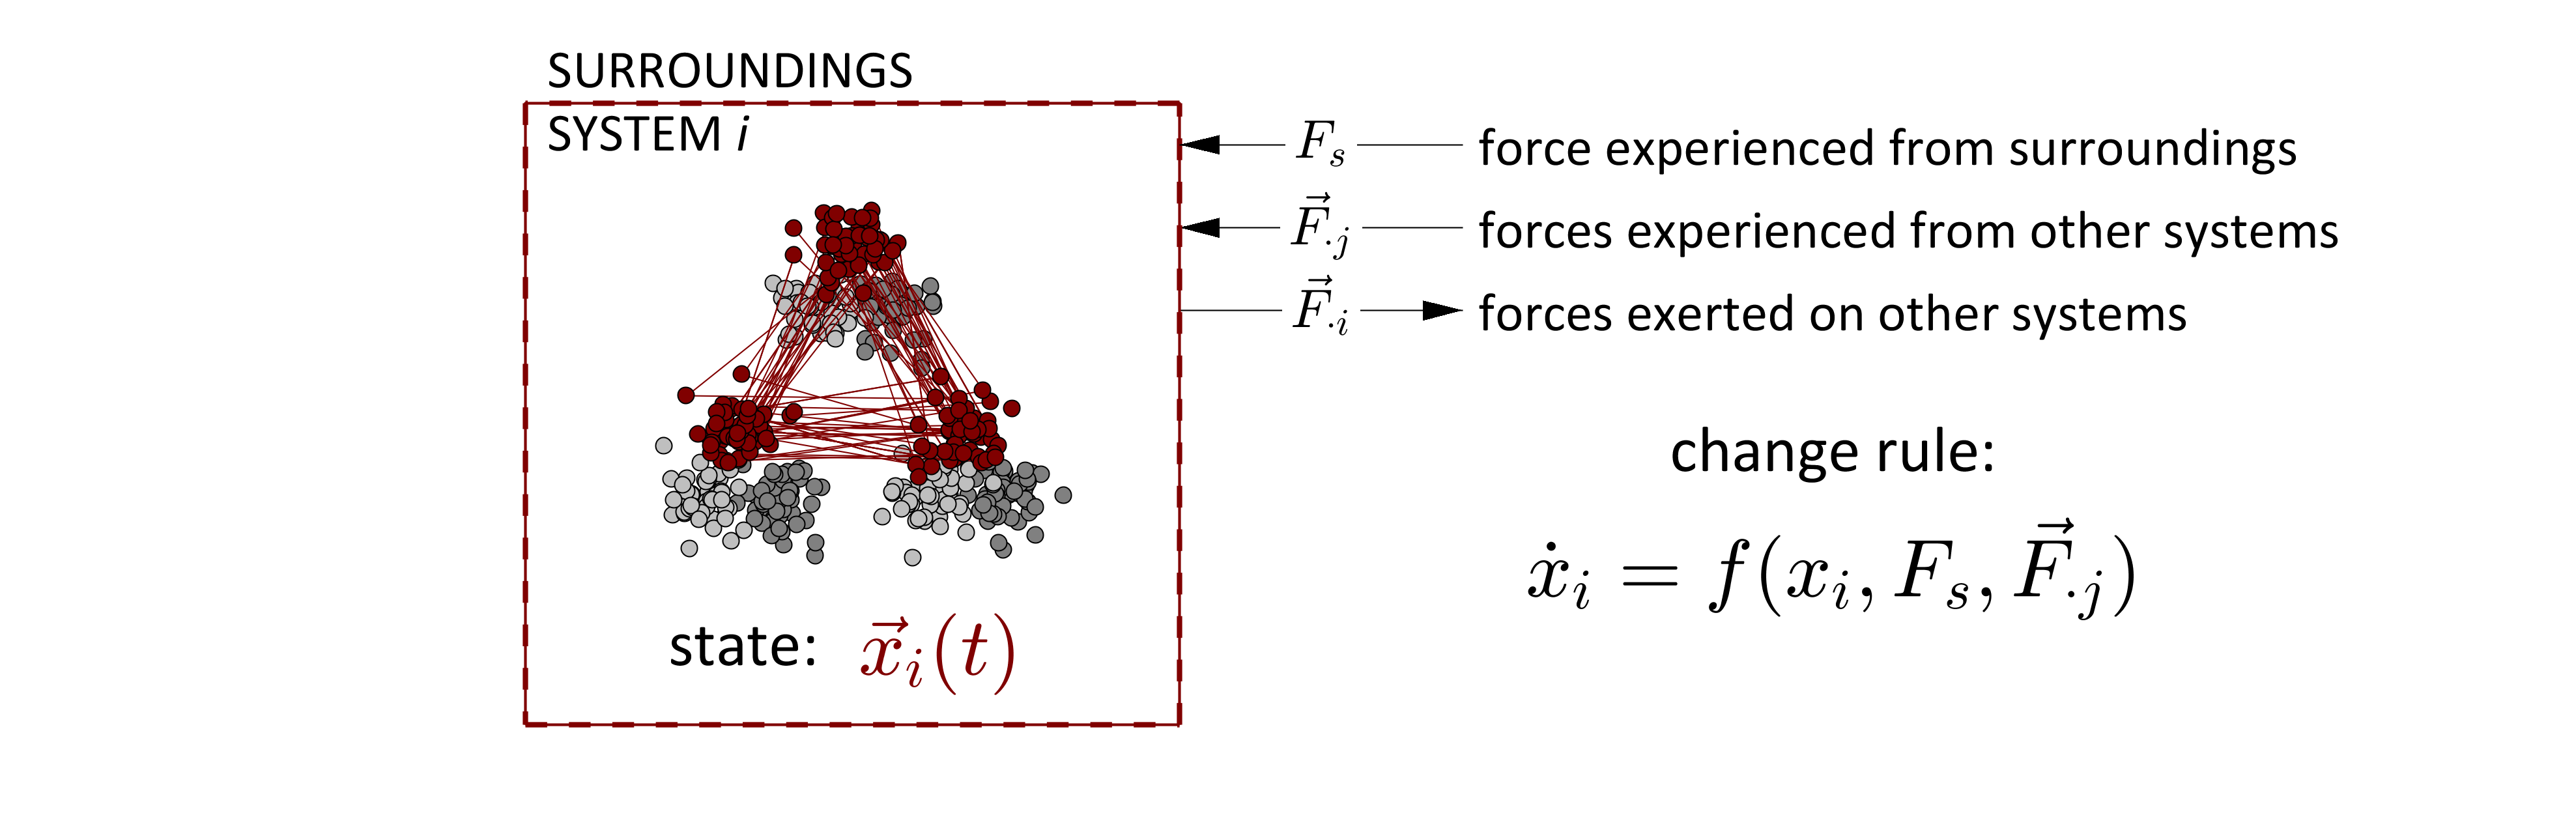
\includegraphics[width=\textwidth]{figures/Tilsen-img11.png}
\caption{\missingcaption}
\label{fig:}
\end{figure}
 

\subsection{System state variables: excitation and phase}

To construct a change rule for system states, we must define the state space. To do this, we reconceptualize the spike-rate of each population, i.e. a time-integration of action potentials, as a macroscopic \textit{order parameter}, \textit{A}. The order parameter \textit{A} is the deviation of the spike rate from a reference value associated with the inactive regime. Furthermore, we conjecture that when a system activates, variation in the order parameter has two components: an oscillation component x\textsubscript{osc}, and an excitation component x\textsubscript{exc}, whose sum is the order parameter, i.e. \textit{A} = x\textsubscript{osc} + x\textsubscript{exc}. We then approximate the oscillation component as a harmonic oscillation with time-varying amplitude and phase angle, i.e. x\textsubscript{osc} = r(t) cos θ(t).The phase variable θ of a system is taken to be 2π{}-periodic, evolves according to an intrinsic system frequency \textit{f}\textsubscript{0}, and is influenced by forces from other systems and the surroundings. The radial amplitude of x\textsubscript{osc} is assumed to be proportional to the excitation component of the system, i.e. r  ${\propto}$ x\textsubscript{exc}. This analysis of \textit{A} is schematized below.  

  
\begin{figure}
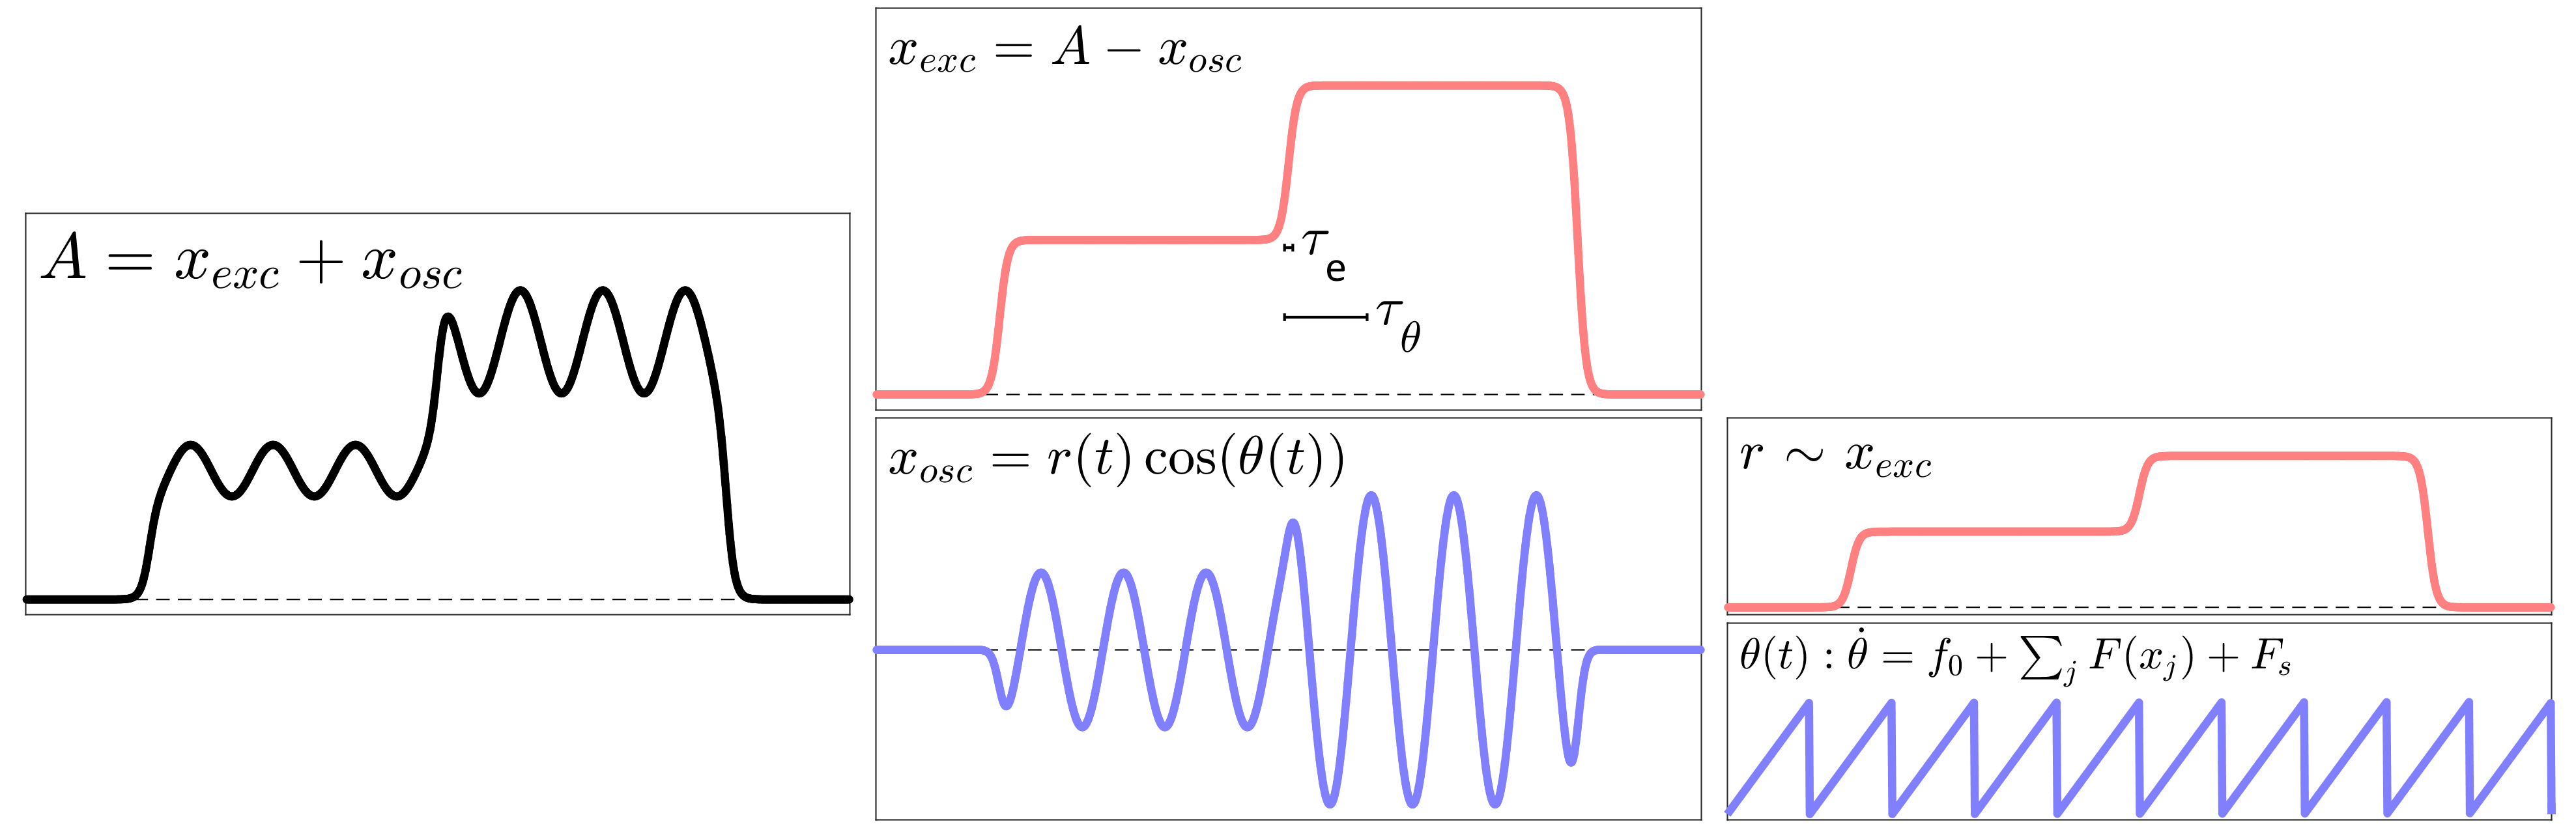
\includegraphics[width=\textwidth]{figures/Tilsen-img12.png}
\caption{\missingcaption}
\label{fig:}
\end{figure}
 

  For exposition, we rename the excitation component x\textsubscript{exc} as (\textit{e}) and refer to phase angle (θ) simply as \textit{phase}. We make a heuristic simplification by assuming the dynamics of \textit{e} and θ are separable due to differences in relevant timescales. This stipulated separation entails that there is a fast timescale τ\textsubscript{e} such that changes in \textit{e} occur over intervals τ\textsubscript{e}, and τ\textsubscript{e} << τ\textsubscript{θ} = 1/\textit{f}, the period of the oscillation. Hence in our analyses of the dynamics of \textit{e} and θ, intermittent abrupt changes in \textit{e} are assumed not to interact directly with θ. Furthermore, the intrinsic frequency \textit{f}\textsubscript{0} is considered to be slowly-varying on utterance timescales, and for some purposes can be conceptualized as a fixed parameter. 

  Given the above construction, the state space for one concept system is the union of subspaces for \textit{e} and θ. We do not attempt to provide a more detailed derivation of these variables and their separation from a microscopic, population-scale model. Nonetheless, we speculate that oscillation arises from intra-population synaptic interactions, intrinsic neuronal dynamics, cortical microcircuit structure, and coupling between neurons and the extracellular medium, whereas excitation relates more directly to the number of neurons which participate in a population oscillation.  

\subsection{Meaning experiences are trajectories in state space}

The utterance \textit{Al drinks coffee} does not “have” a meaning. An utterance can only \textit{have} a meaning if we presuppose that meanings are objects contained in words. We reject these object and containment metaphors. Instead, meanings are experiences which correspond to trajectories in concept system \textit{e},θ space. The conventional object and o/el trajectory metaphors are contrasted below. In o/el terms, a meaning experience associated with a single concept arises when two conditions are met: (i) a stable periodic trajectory occurs in the θ subspace associated with a concept, for an interval of time on the order of τ\textsubscript{θ}, and (ii) the excitation of the concept exceeds a threshold value λ\textsubscript{e}. When \textit{e} > λ\textsubscript{e} we refer to the system as \textit{excited}; when 0 < \textit{e} < λ\textsubscript{e}, we refer to the system as \textit{active}; when e = 0 we refer to the system as \textit{inactive}. The phase θ of an inactive system is undefined, because by definition the inactive state entails no collective oscillation. 

  
\begin{figure}
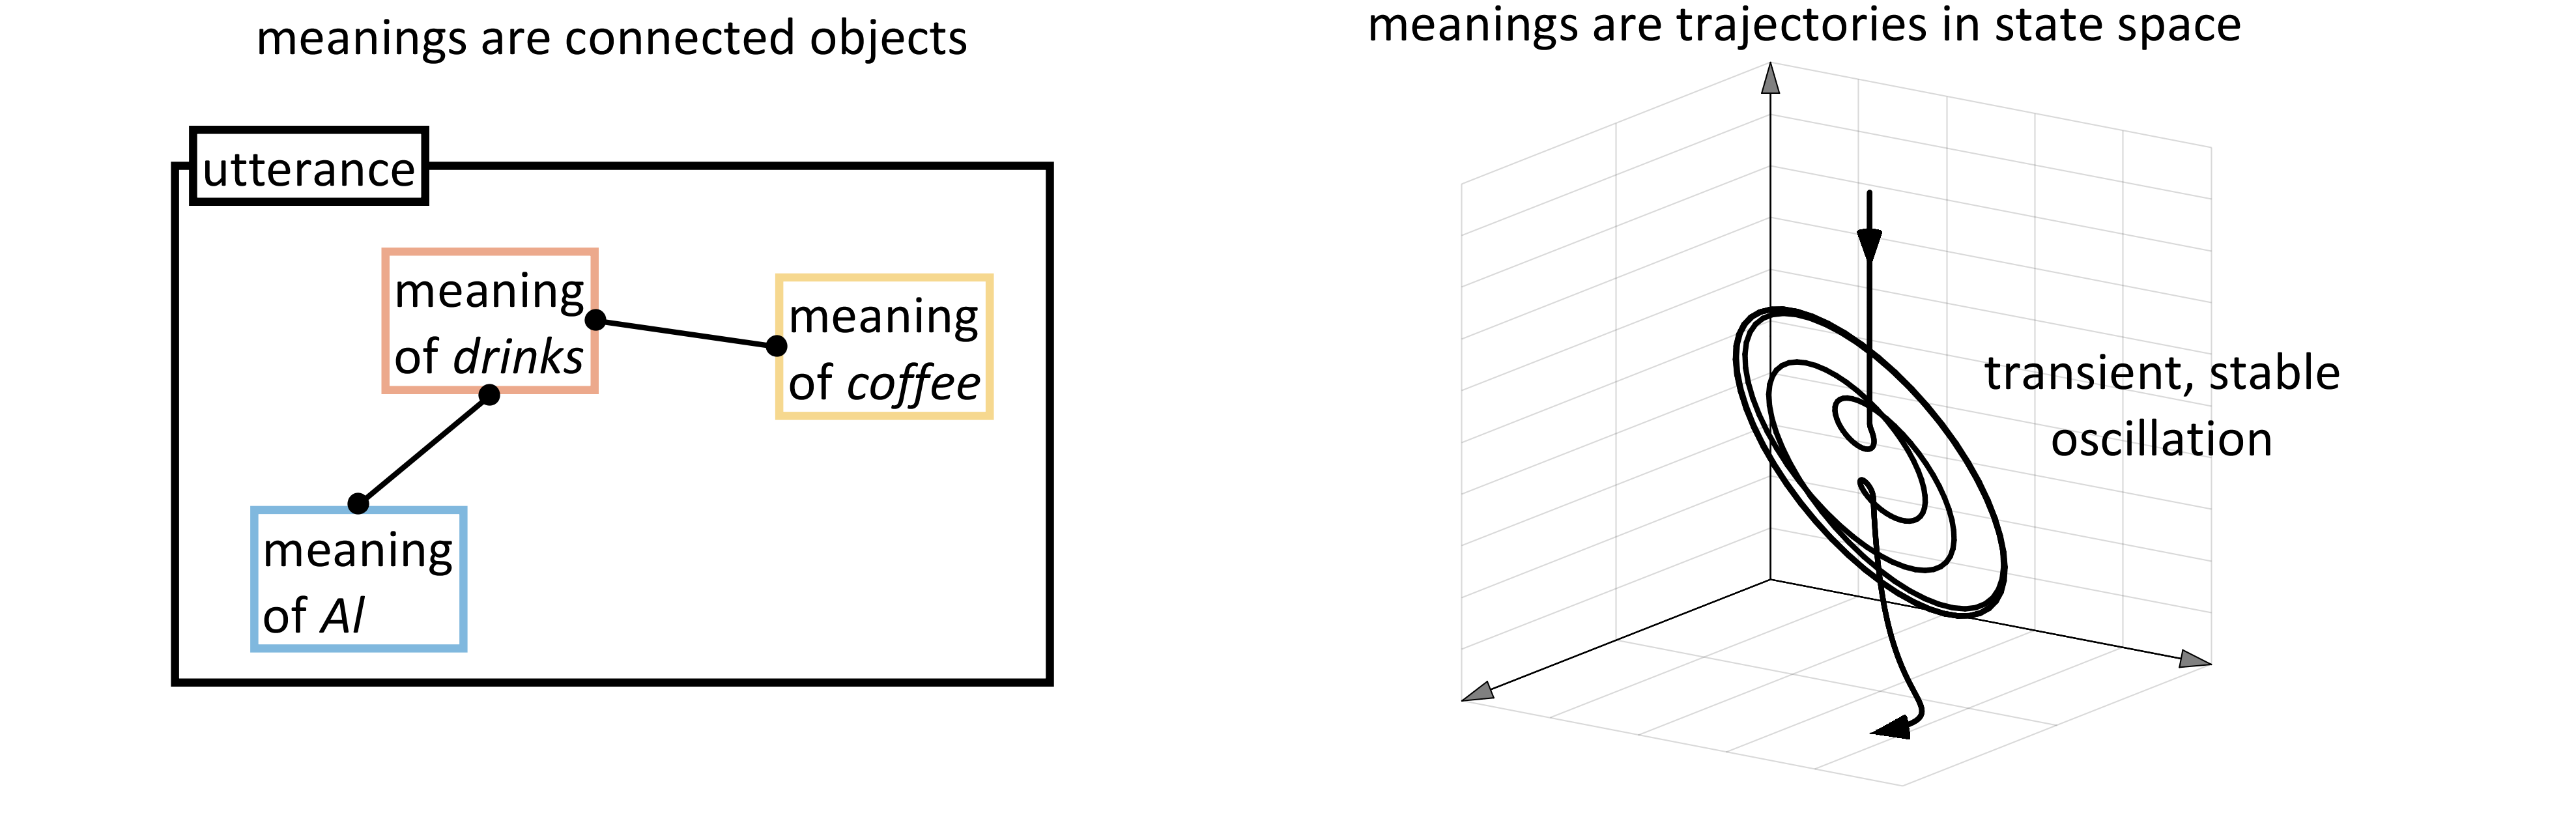
\includegraphics[width=\textwidth]{figures/Tilsen-img13.png}
\caption{\missingcaption}
\label{fig:}
\end{figure}
 

  The \textit{e},θ state space is 2-dimensional for one concept system, and 2\textit{n}{}-dimensional for \textit{n} concept systems. Moreover, when \textit{n} concept systems are excited, a relational meaning experience associated with those systems is a stable periodic orbit in the \textit{n}{}-dimensional θ subspace. Typically we are interested in meaning experiences associated with systems whose \textit{e} > λ\textsubscript{e}, i.e. excited systems. We will sometimes refer to these as \textit{attended} meanings, because we imagine that the relevant concept systems have \textit{e} values which are sufficient to support conscious attention to a meaning experience. In contrast, subconscious experience of meaning occurs via active, unexcited systems.

  Note that \textit{e} and θ state variables are analytical constructs which we can attempt to derive from a higher-dimensional microscale state space. This derivation procedure uses methods of projection and integration in order to reduce dimensionality. Accordingly, the state space is always constructed \textit{ad hoc} to accommodate the systems which we consider relevant for a given analysis. The state space construction procedure is (i) stipulate concept systems; (ii) construct a space with \textit{e} and θ dimensions for each system; (iii) construct the union of these spaces by combining them orthogonally. The picture to have in mind is below. 

  
\begin{figure}
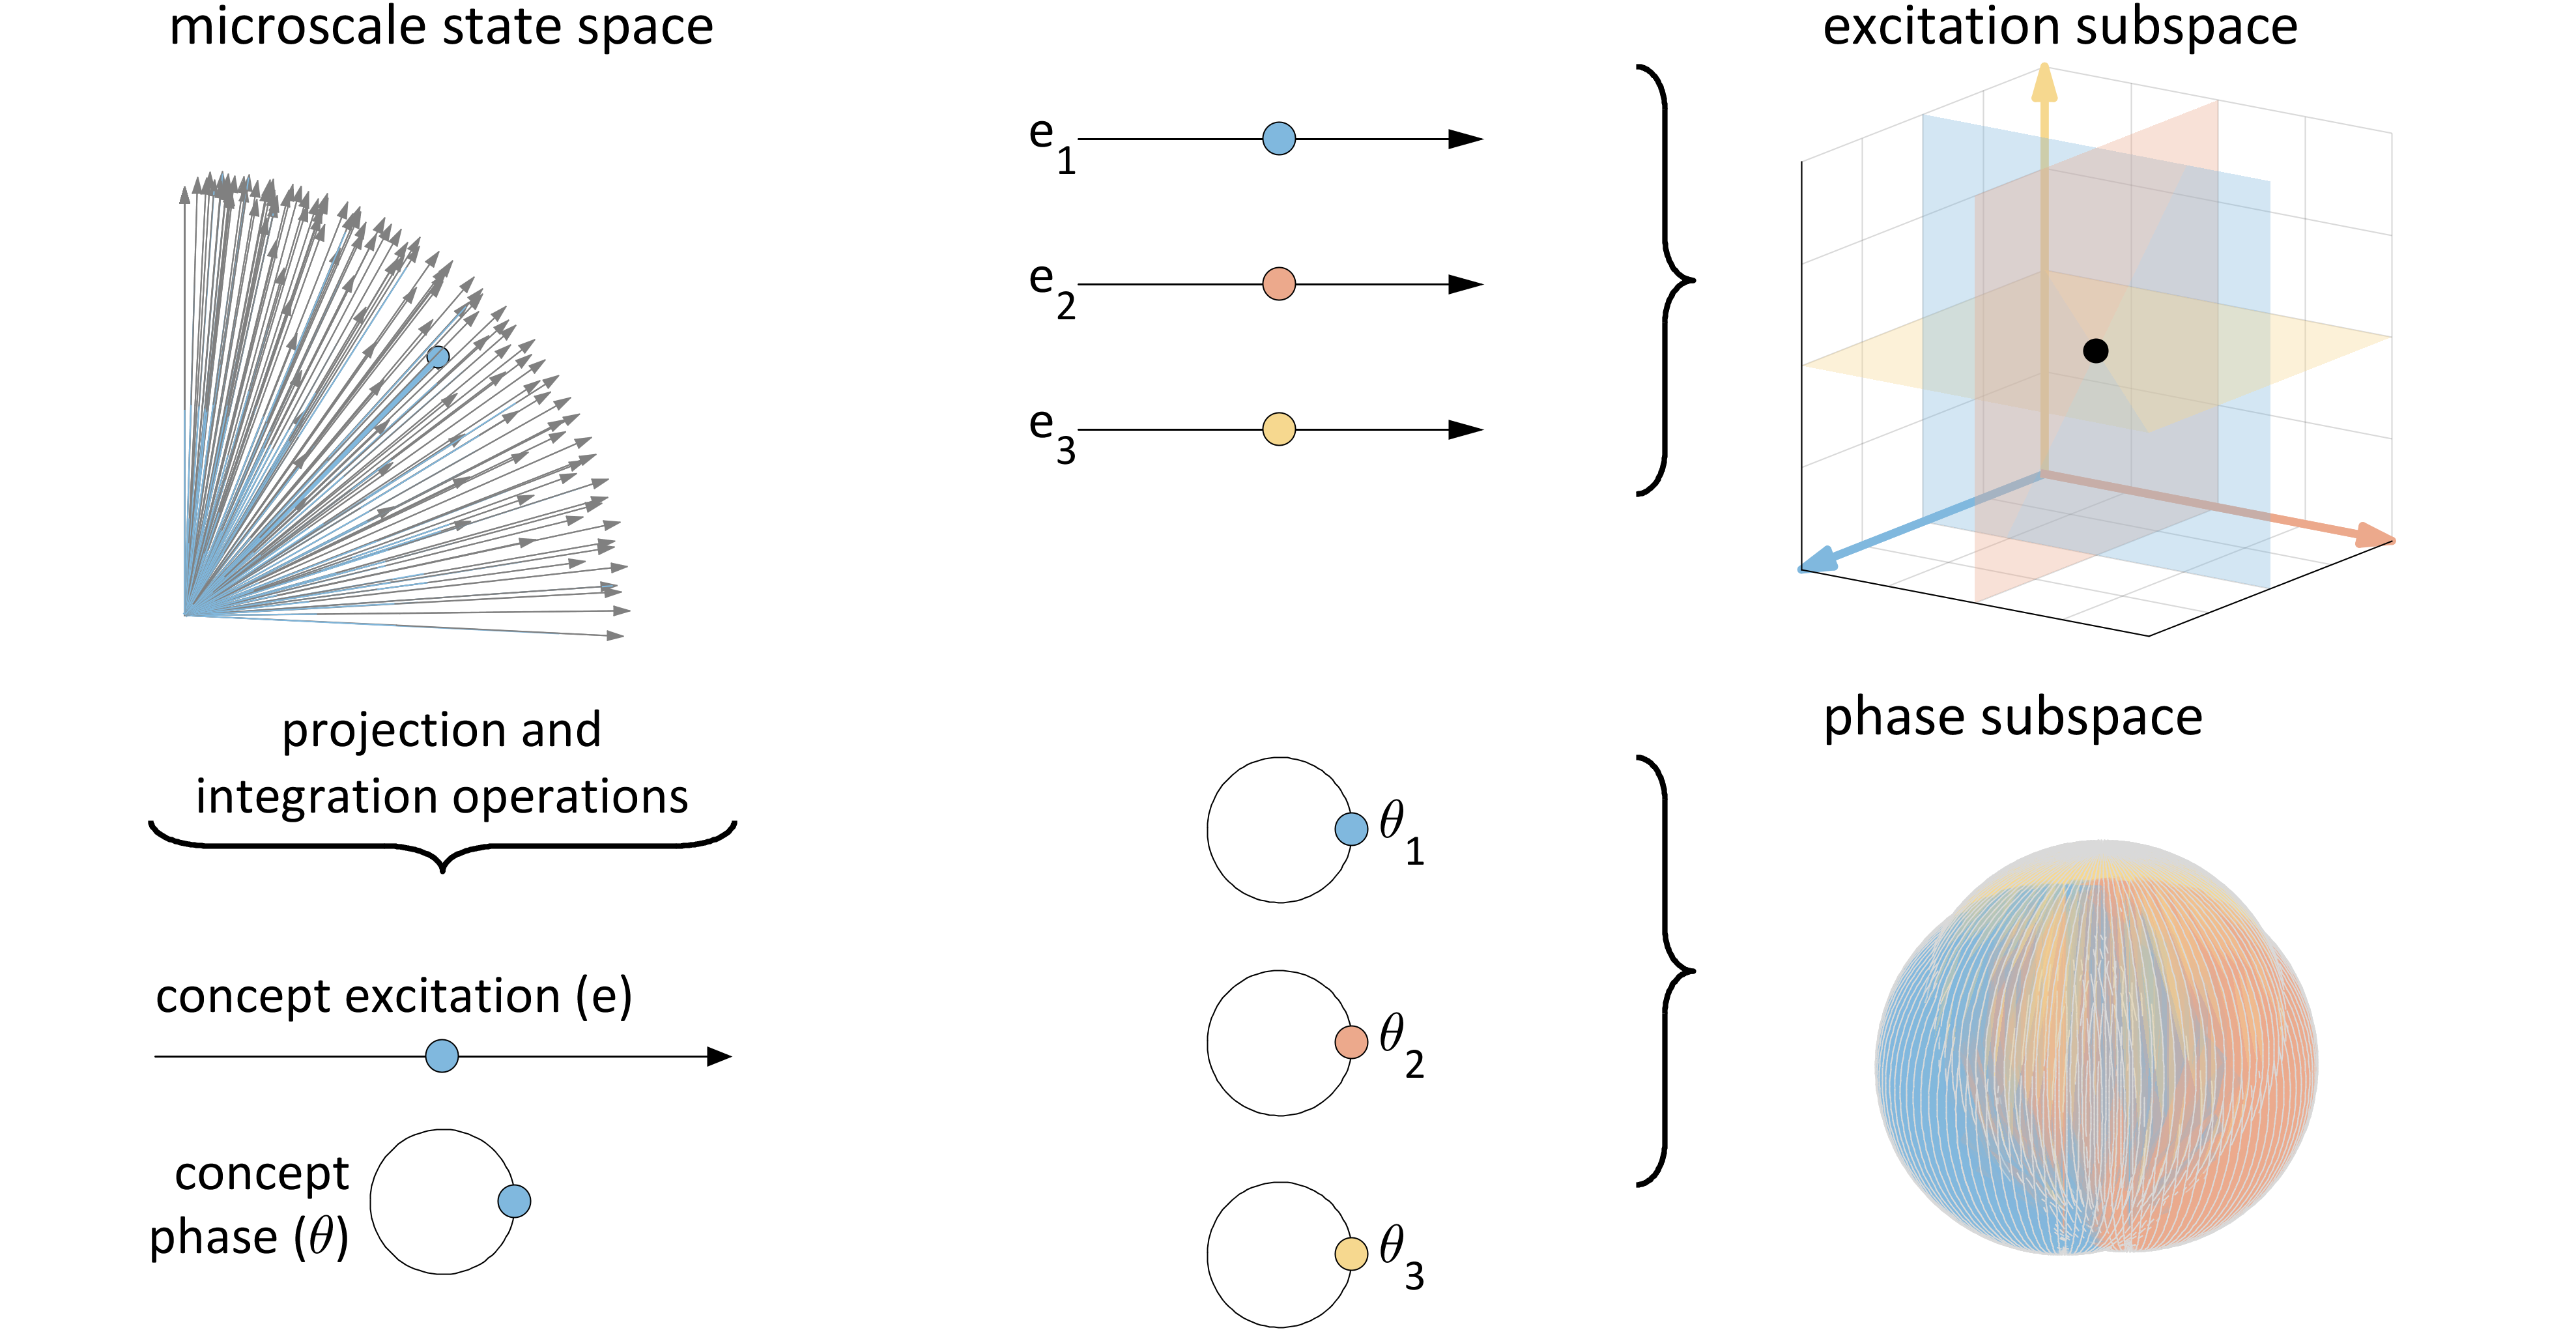
\includegraphics[width=\textwidth]{figures/Tilsen-img14.png}
\caption{\missingcaption}
\label{fig:}
\end{figure}
 

  The state space is neither permanent nor a physical space. It is a heuristic tool that we construct strategically to meet the needs of a given analysis. Describing [Al], [drinks], and [coffee] with orthogonal excitation and phase variables is useful because it provides a coarse model of the much higher-dimensional states of neural populations. Conceptualizing meaning experiences as trajectories in the e,θ space opens up a new approach to reasoning about linguistic phenomena.

\subsection{Relational meaning experiences are relative phase configurations}

Individual concept meaning experiences rarely occur in isolation. The production of \textit{Al drinks coffee} is associated with simultaneous excitation of concepts [Al], [drinks], and [coffee]. Yet simultaneity of excitation is not sufficient for understanding the \textit{relational} character of meaning experiences. This is obvious from consideration of utterances such as \textit{Al likes Bo} and \textit{Bo likes Al}, where the same concepts are excited and yet different relational meanings are experienced. Since we do not experience both of these relational meanings simultaneously, there must be a mechanism which distinguishes system states in which [Al] and [Bo] have different relations to [likes]. Moreover, this mechanism should also govern the relations of [Al] and [coffee] to [drinks] in \textit{Al drinks coffee}, as well as any arbitrary relations of this sort. 

  To that end we propose a \textit{principle of relational meaning}: relational meaning experiences are stable relative phase configurations. Recall that relative phase φ is defined as the antisymmetric difference of phases, i.e. φ\textsubscript{ij} = θ\textsubscript{i} - θ\textsubscript{j} = -φ\textsubscript{ji}. For exposition we often refer to φ without indices and interpret this as the absolute value of relative phase, i.e. {\textbar}φ{\textbar} = {\textbar}θ\textsubscript{i} – θ\textsubscript{j}{\textbar}. Furthermore, we pursue a strong hypothesis that all relational meaning experiences are associated with a stable states in which φ ${\approx}$ 0 or π, which we call \textit{in-phase} and \textit{anti-phase}, or \textit{proximal} and \textit{distal} φ configurations, respectively. More precisely, for any pair of concept systems \textit{i} and \textit{j}, a relational meaning experience occurs when both systems are excited \{e\textsubscript{i}, e\textsubscript{j}\} > λ\textsubscript{e} and have a stable relative phase such that {\textbar}φ\textsubscript{ij}{\textbar} ${\approx}$ \{0, π\} and dφ\textsubscript{ij}/dt ${\approx}$ 0. Specifically, we hypothesize that in-phase states (φ ${\approx}$ 0) are associated with agent-action relations, e.g. [Al][drinks], and that anti-phase states (φ ${\approx}$ π) are associated with patient-action relations, e.g. [drinks][coffee]. These are summarized in the {\tablebelow}. Many additional φ-relation hypotheses are developed subsequently.

  \begin{table}
\begin{tabularx}{\textwidth}{XXll}
  \lsptoprule
  \multicolumn{2}{c}{\textbf{conceptual systems}} & 
  \textbf{semantic relations} & 
  \textbf{$\varphi$ configurations}\\
  \midrule{}
  [Al] & [drink] & agent-action & in-phase: φ ${\approx}$ 0\\{}
  [coffee] & [drink] & patient-action & anti-phase: φ ${\approx}$ π\\
  \lspbottomrule
  \end{tabularx}
\caption{\missingcaption}
\label{tab:key:}
\end{table}

  The φ configurational basis for differences in relational meaning between [Al][drinks] and [coffee][drinks] is illustrated below. Crucially, [Al][drinks] and [coffee][drinks] φ configurations remain constant despite the fact that all three θ variables are changing. Constant φ, when stable over time periods on the order of τ\textsubscript{θ}, gives rise to the experience of relational meaning between systems, as long as those systems are excited. Note that φ configurations are periodic trajectories in θ space, but we can also construct a φ space in which a stable φ configuration is a point. Moreover, because θ dimensions are circular, wrapping around the interval [0, 2π], φ patterns can also be represented as a static phase difference on a unit circle, as below. In such representations we choose some system as a reference, and the phase angles of all other systems are shown relative to the phase of the reference system. For visual clarity, we depict systems with a φ=0 configuration as having a small φ separation, as with [Al] and [drinks] below.

  
\begin{figure}
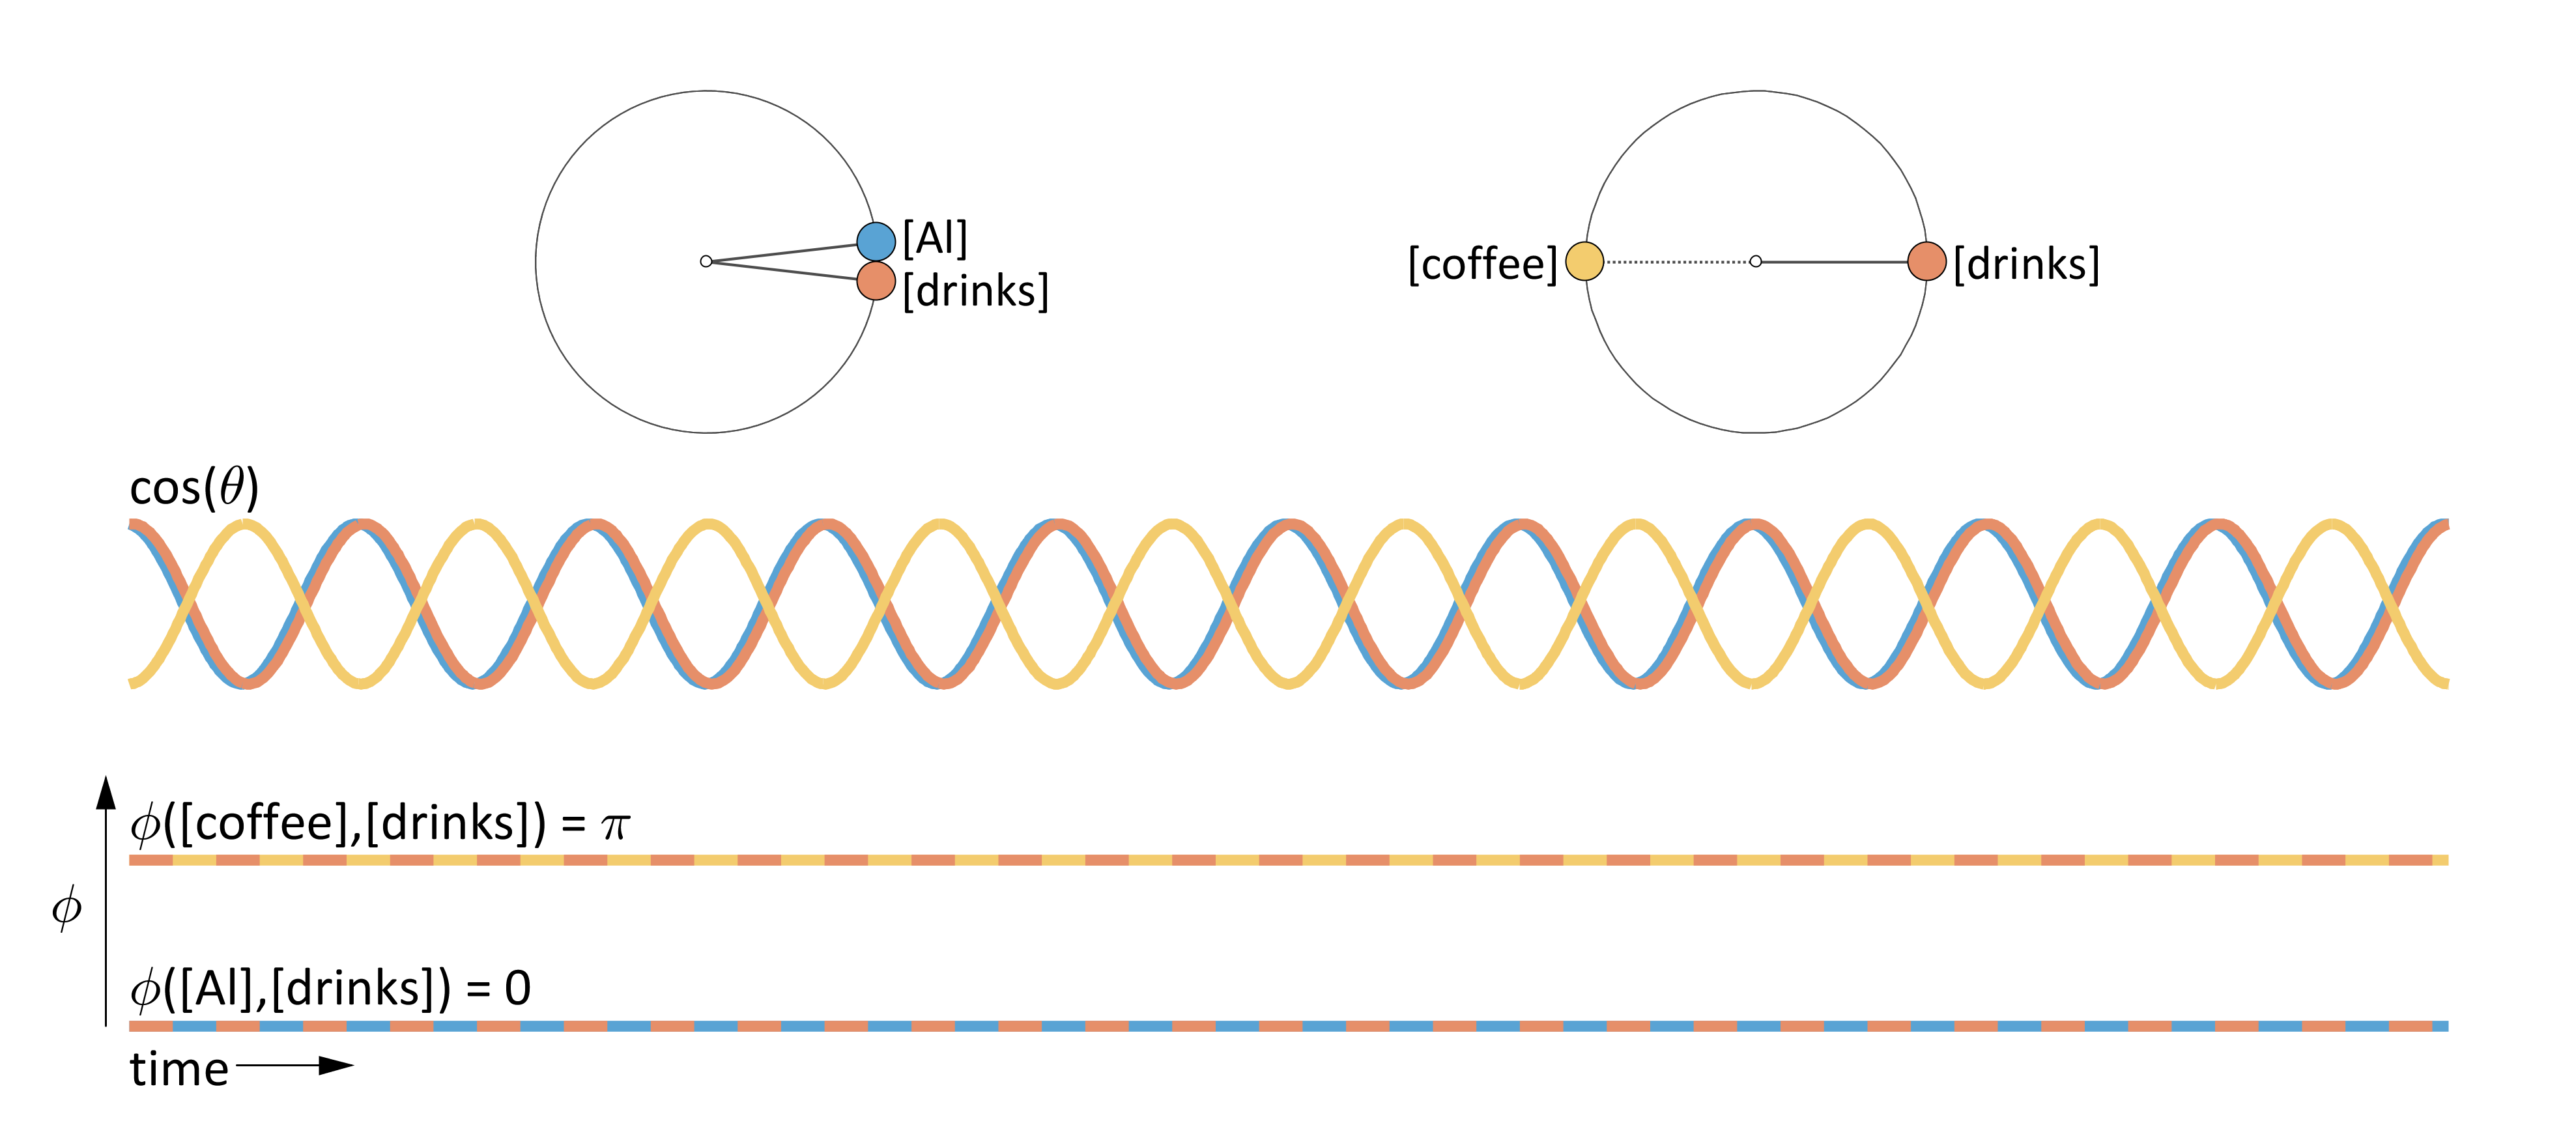
\includegraphics[width=\textwidth]{figures/Tilsen-img15.png}
\caption{\missingcaption}
\label{fig:}
\end{figure}
 

  The principle of relational meaning requires relational meaning experiences to be \textit{stable} φ configurations. Here \textit{stable} means that φ, when perturbed, returns to an equilibrium value (0 or π) on a timescale which is substantially less than τ\textsubscript{θ}. Fluctuations constantly perturb θ variables of systems and hence perturb φ. A stabilizing mechanism is thus required to force φ back an equilibrium value. 

  What is the stabilizing mechanism? Our microscopic model suggests that synaptic projections between concept systems and other systems could accomplish this stabilization. By integrating over interpopulation synaptic projections we can derive macroscopic \textit{coupling forces}, which serve to stabilize φ. However, if these forces act directly between concept systems, there is a problem…

\subsection{Direct interactions between conceptual systems are unlearnable and inflexible.} 

Lets imagine that a direct interaction between [Al] and [drinks] concept systems were indeed responsible for stabilizing their φ configuration. On the basis of our microscale conception, such interactions must be learned: macroscopic forces are derived from synaptic weights (i.e. efficacy of neurotransmitter release/uptake), connectivity patterns, etc. between populations. Learning is an evolution of these variables on supra-utterance timescales. Moreover, the interaction, if a stabilizing one, would need to be fairly strong, otherwise moderate perturbations would overcome the equilibration forces. 

  There are two problems with the direct coupling scenario. The first involves learnability. Two different types of interactions between [Al] and [drinks] would need to be learned, i.e. an in-phase and anti-phase interaction for the agent and patient roles, respectively. Moreover, these two types of interaction would need to be learned for all \textit{pairs} of concepts: for \textit{n} concept systems there are 2\textit{n}\textsuperscript{2} interactions. The second problem involves flexibility. If the learned stabilizing interactions are too strong, then there is a danger that excitation of one concept system will always cause other concept systems that it interacts with to become excited. For example, imagine that when [Al] becomes excited, direct interaction forces excite [drinks] and [coffee] as well. This is a problem if one wants to experience the meaning of \textit{Al eats granola}, for example. With direct interactions between concept systems, system trajectories would be prone to seizures in which all concept systems become excited. The solutions to the flexibility and learnability problems are provided by syntactic systems.

\section{Syntactic systems}

Syntactic systems are the primary mechanism for stabilizing φ configurations of concept systems. There are two basic aspects of this mechanism. First, concept systems resonate with syntactic systems through mutual positive feedback. We refer to this as \textit{resonance} because syntactic systems have strong, asymmetric interactions with concept systems. Second, syntactic systems couple strongly to other syntactic systems. Hence syntactic systems can organize and stabilize φ configurations between concept systems, without requiring strong direct coupling between concept systems. Syntactic systems provide an \textit{indirect}, \textit{flexible} mechanism for stabilizing relational meaning, one which does not rely on learning direct interactions between concepts. Henceforth we abbreviate concept systems as \textit{c-systems}, and syntactic systems as \textit{s-systems}. 

\subsection{Microscopic conception of syntactic and conceptual systems}

Both s- and c-systems have \textit{e} and θ state variables, and these are derived in the same way from a microscale conceptualization of populations. But the microscopic pictures of c-systems and s-systems differ in some important ways which help resolve the learnability and flexibility problems. First, for concepts we imagine a large, distributed population of neurons. Each individual c-system is a subpopulation of this full population, and despite substantial overlap of these subpopulations, c-systems can be distinguished from each other on the basis of their interactions with other systems and the sensorimotor surroundings. On the macroscale, the primary mechanism of learning is not “adding” new c-systems, but rather differentiating and blending existing c-systems. On the microscale this entails that new sub-populations are not “created”, but rather new patterns of interaction arise with the sensorimotor surroundings and other conceptual systems. Interactions between c-systems are presumed to be relatively weak: c-systems can activate other c-systems (this is often called \textit{priming}), but typically do not excite other c-systems.

  
\begin{figure}
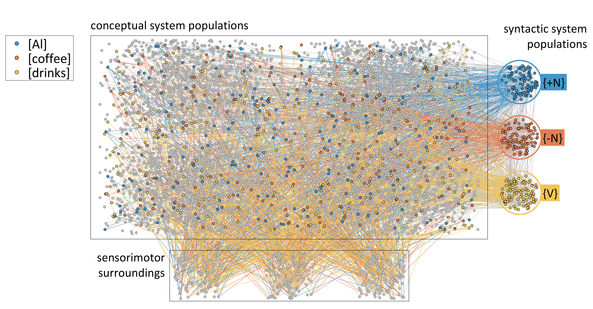
\includegraphics[width=\textwidth]{figures/Tilsen-img16.png}
\caption{\missingcaption}
\label{fig:}
\end{figure}
 

  In contrast to the full population of c-systems, the full population of s-systems is spatially localized, possibly in the inferior frontal gyrus. Individual s-systems, i.e. subpopulations of the full s-system population, overlap to lesser degree with each other than c-systems do, and interact more strongly because of their spatial localization. 

  The c- and s-system populations project to one another, and under certain conditions c-system populations may resonate with s-system populations, a phenomena we refer to as \textit{cs-resonance}. We assume that the capability for cs-resonance is phylogenetic, but in development, different c-systems become preferentially biased to resonate with different types of s-systems. Furthermore, we speculate that the effects of general learning mechanisms (e.g. Hebbian spike-timing dependent synaptic plasticity), when integrated on supra-utterance timescales, differentiate the full syntactic population into various s-system subpopulations. Biases for in-phase and anti-phase coupling interactions between s-system populations are learned in this manner, giving rise to a grammar of φ coupling. A more thorough discussion of learning in the o/el framework is undertaken later on, but the primary focus of this book is the analysis of utterance-timescale patterns in speech.

\subsection{Conceptual systems resonate with syntactic systems}

The cs-resonance mechanism can be understood as follows. First, forces from the surroundings activate a c-system and a corresponding s-system. These systems begin to resonate weakly, in a positive mutual feedback interaction. Microscopically, the positive feedback resonance mechanism derives from integrating the effects of excitatory-to-excitatory interpopulation projections between an s-system and c-system. Because these projections are excitatory, resonating c- and s-systems always have an in-phase φ-relation. 

  Recall that activation implies a collective oscillation, but not stability of θ′ and not necessarily an \textit{e} value sufficient for a meaning experience. In general many c-systems may be active and may compete for resonance with a given s-system; surroundings forces influence this competition as well. The competition from other c-systems and surroundings forces can potentially destabilize a newly formed resonance between c- and s-systems. We thus imagine a pre-stable phase of production in which interaction between a c- and s-system may or may not lead to a strong cs-resonance. If positive feedback between the c- and s-system is sufficiently strong relative to destabilizing forces, the c- and s- system abruptly become \textit{excited}, which entails that the s-system \textit{e} value exceeds a threshold, as shown below. The \textit{e}{}-value of the c-system also increases, but for reasons that become clear we need make no specific assumptions about c-system \textit{e}{}-values relative to other c- or s-systems. We henceforth refer to a pair of resonating c- and s-systems (whether excited or merely active) as a \textit{cs-system}, or simply a \textit{system}. In the {\figurebelow}, the c-system [coffee] resonates with the s-system \{N\}, and this gives rise to a stable, excited cs-system.

  
\begin{figure}
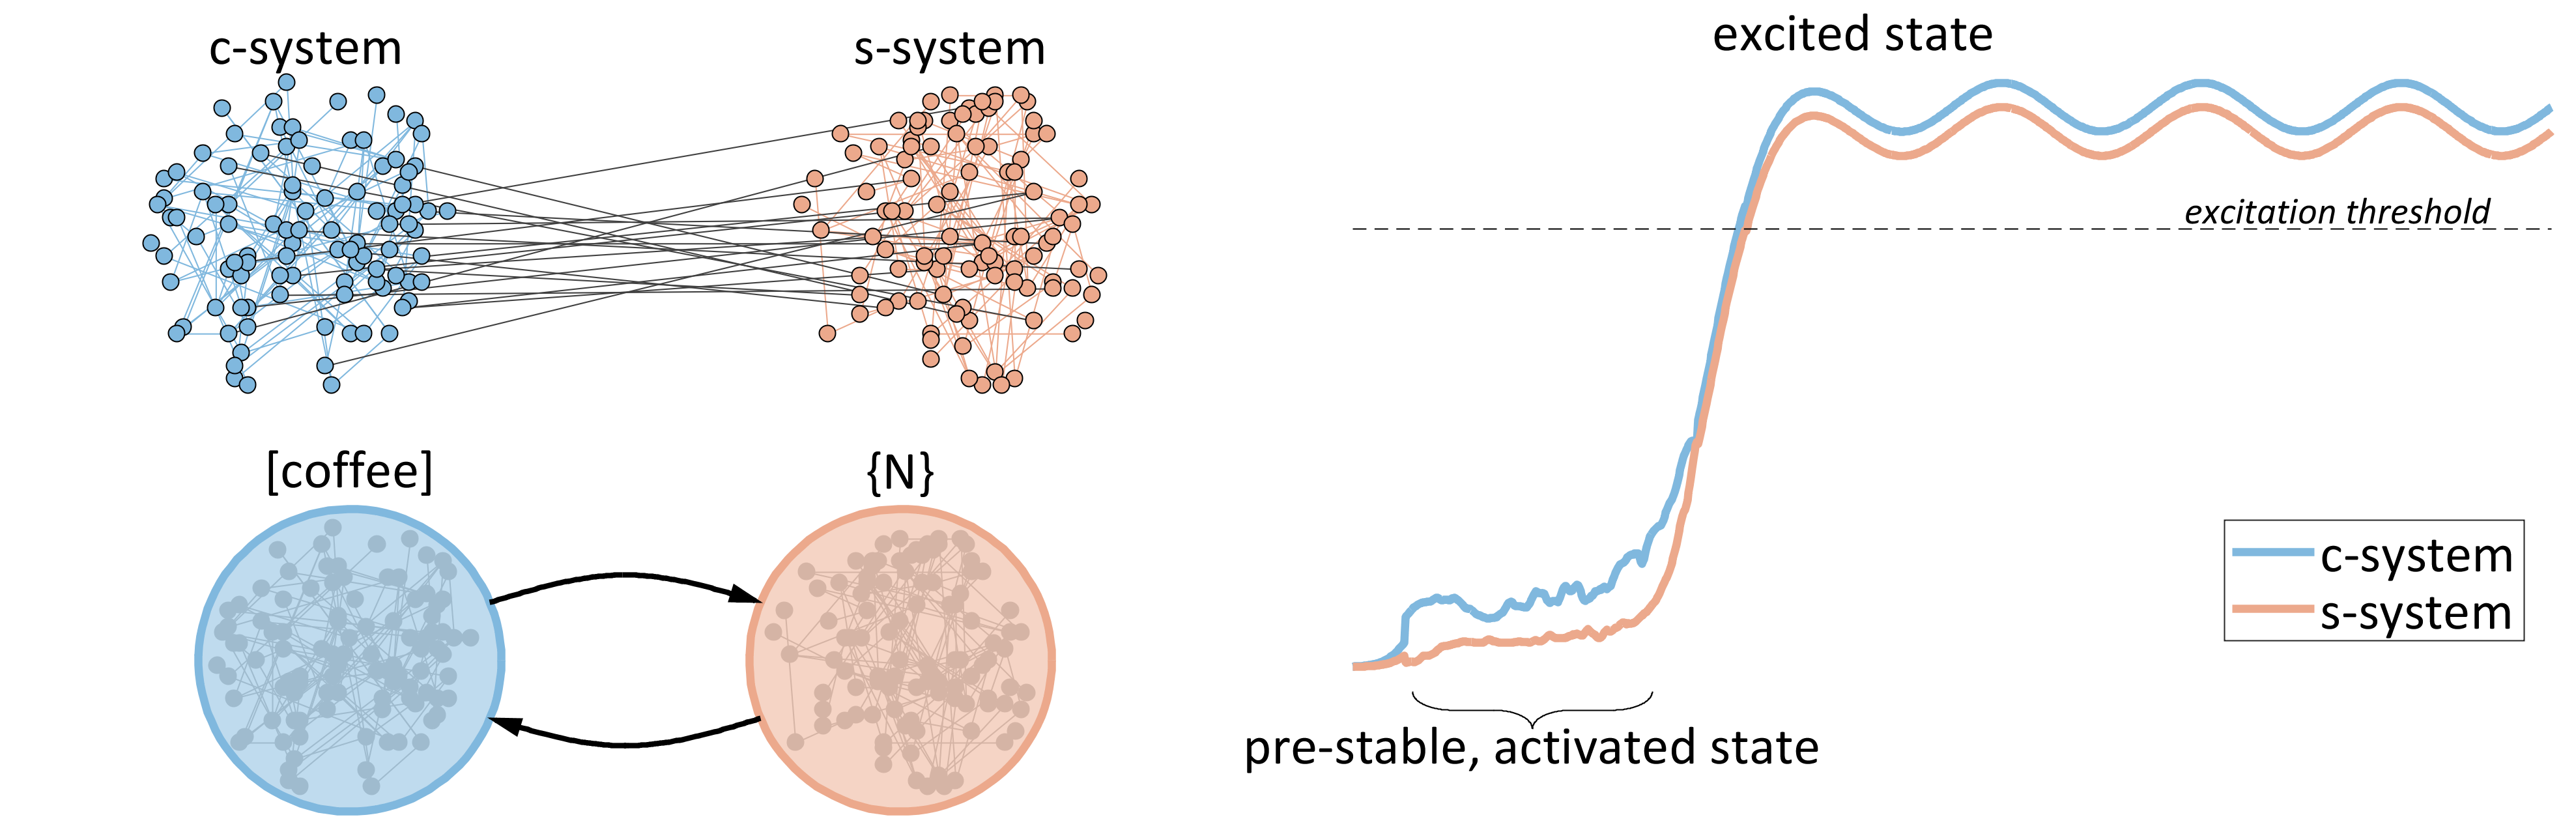
\includegraphics[width=\textwidth]{figures/Tilsen-img17.png}
\caption{\missingcaption}
\label{fig:}
\end{figure}
 

  A key diagnostic of cs-system excitation is intrapopulation and interpopulation spectral coherence, a concept which we develop in more detail later on. Moreover, the stabilization of φ entails an augmentation of \textit{e}. The excitation threshold plays an important role in a variety of analyses we develop subsequently. When a cs-system has below-threshold excitation (i.e. the system is active but not excited), the system cannot participate in a stable φ configuration with other cs-systems and hence cannot evoke an attended relational meaning experience. In general, we imagine that there are many active but unexcited cs-systems, before and during production. Thus, in the production of an utterance such as \textit{Al drinks coffee}, the excitation of [Al], [drinks], and [coffee] is merely the tip of an iceberg: a large amount of subthreshold activity occurs below the surface.

\subsection{Coupling force types and valence} 

To classify interactions between systems, we distinguish two types of coupling and two coupling valences. Relative phase coupling (φ-coupling) is an interaction that depends on relative phase φ and influences θ variables. The {\figurebelow} shows the phases of two systems on a phase circle, which is the space of possible phases. The effects of the relative phase (φ) coupling force are shown by the arrows: an attractive φ-force drives θ variables (which are also rotating counterclockwise) toward one another, resulting in a decrease in φ; a repulsive φ-force drives θ variables away from one another, resulting in an increase in φ. The coupling force is associated with a periodic sinusoidal potential function V(φ), such that  $F\left(\varphi \right)=\frac{-\mathit{dV}\left(\varphi \right)}{\mathit{d\varphi} }$ . The effect of the force on φ is analogous to a ball rolling down a hill while submerged in a viscous fluid, where the viscous force perfectly compensates for inertia: the force causes φ to change until it reaches the stable equilibrium of 0 (attractive force) or ±π (repulsive force), where it stops. Because θ is a periodic variable, it is convenient to map φ to the interval [-π,+π]. 

  
\begin{figure}
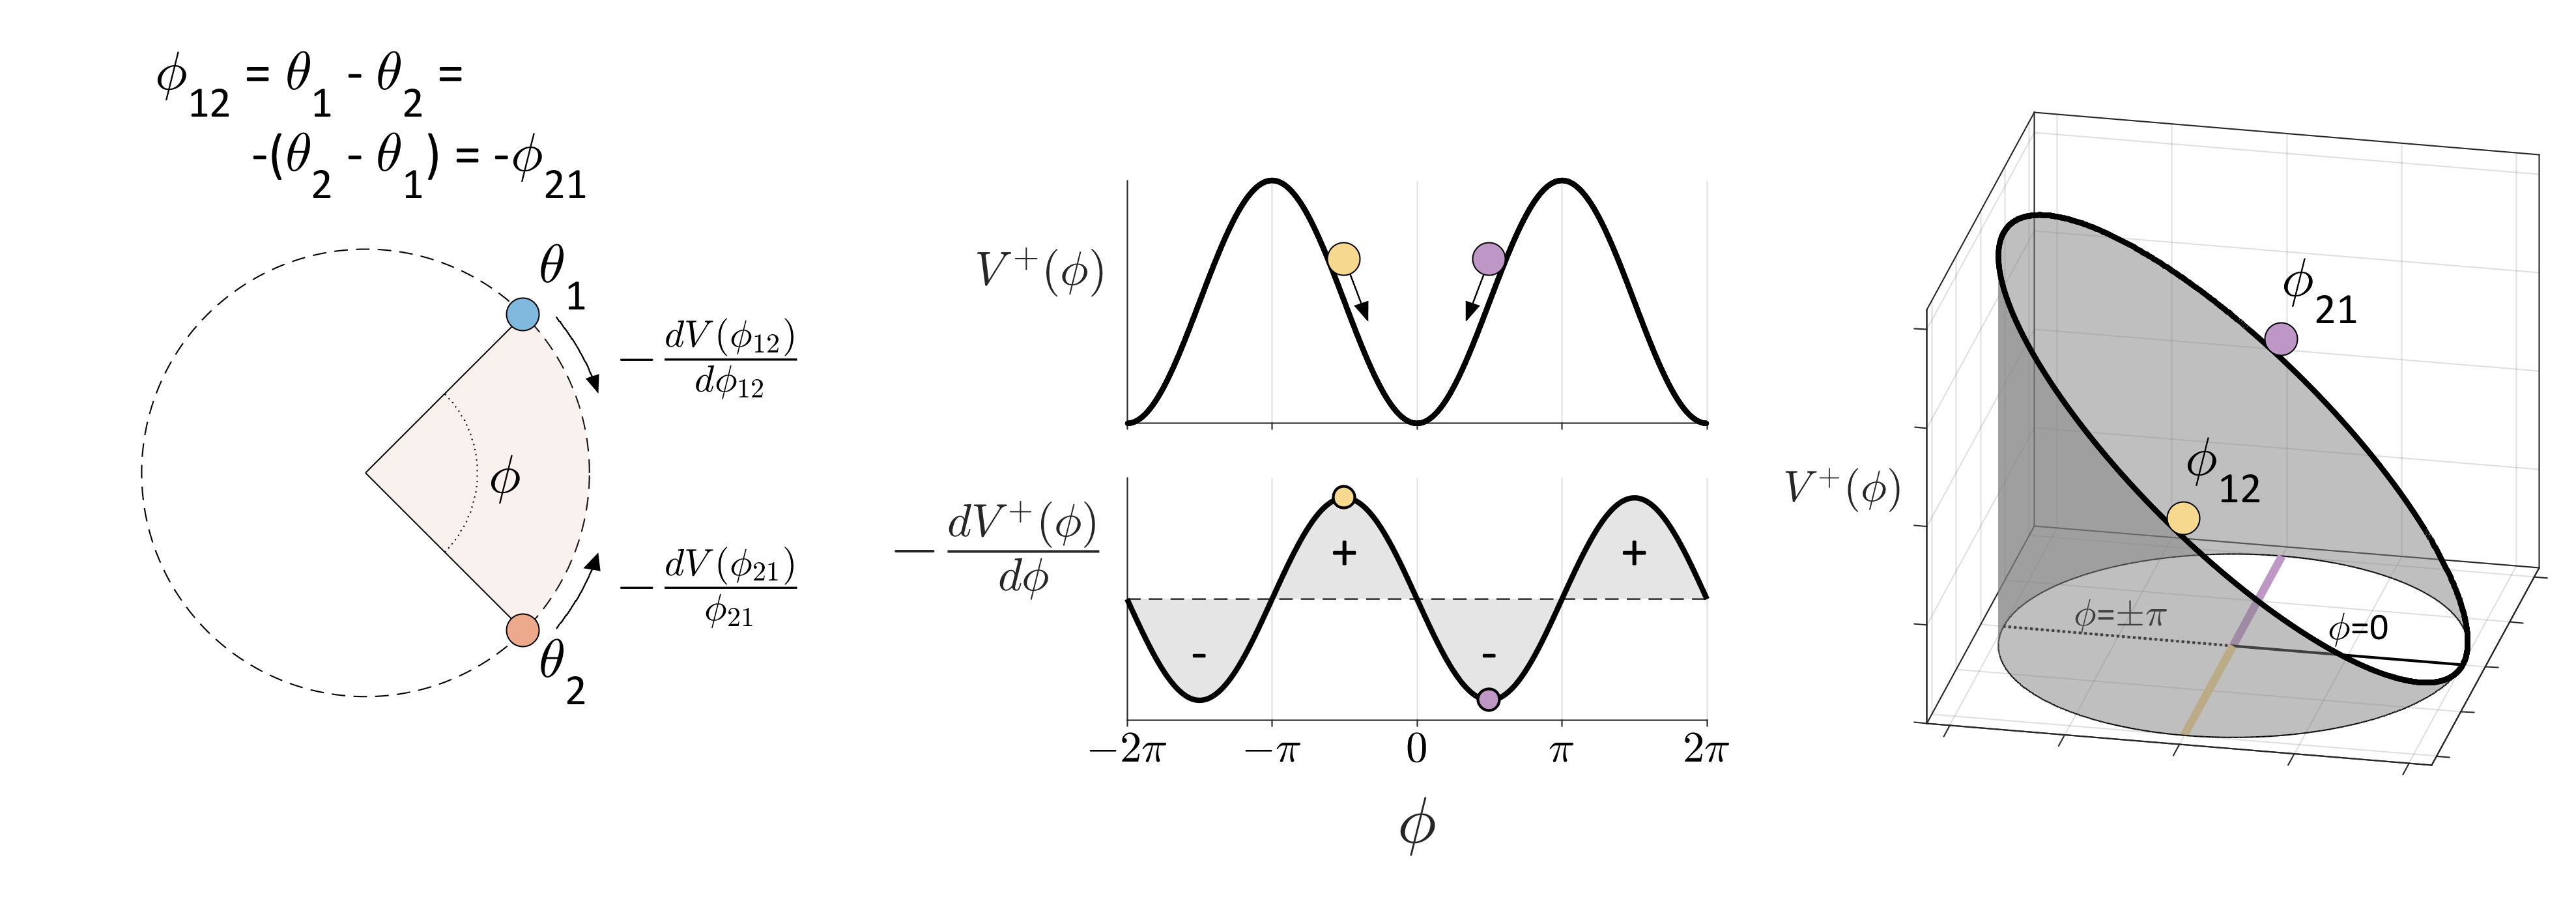
\includegraphics[width=\textwidth]{figures/Tilsen-img18.png}
\caption{\missingcaption}
\label{fig:}
\end{figure}
 

  
\begin{figure}
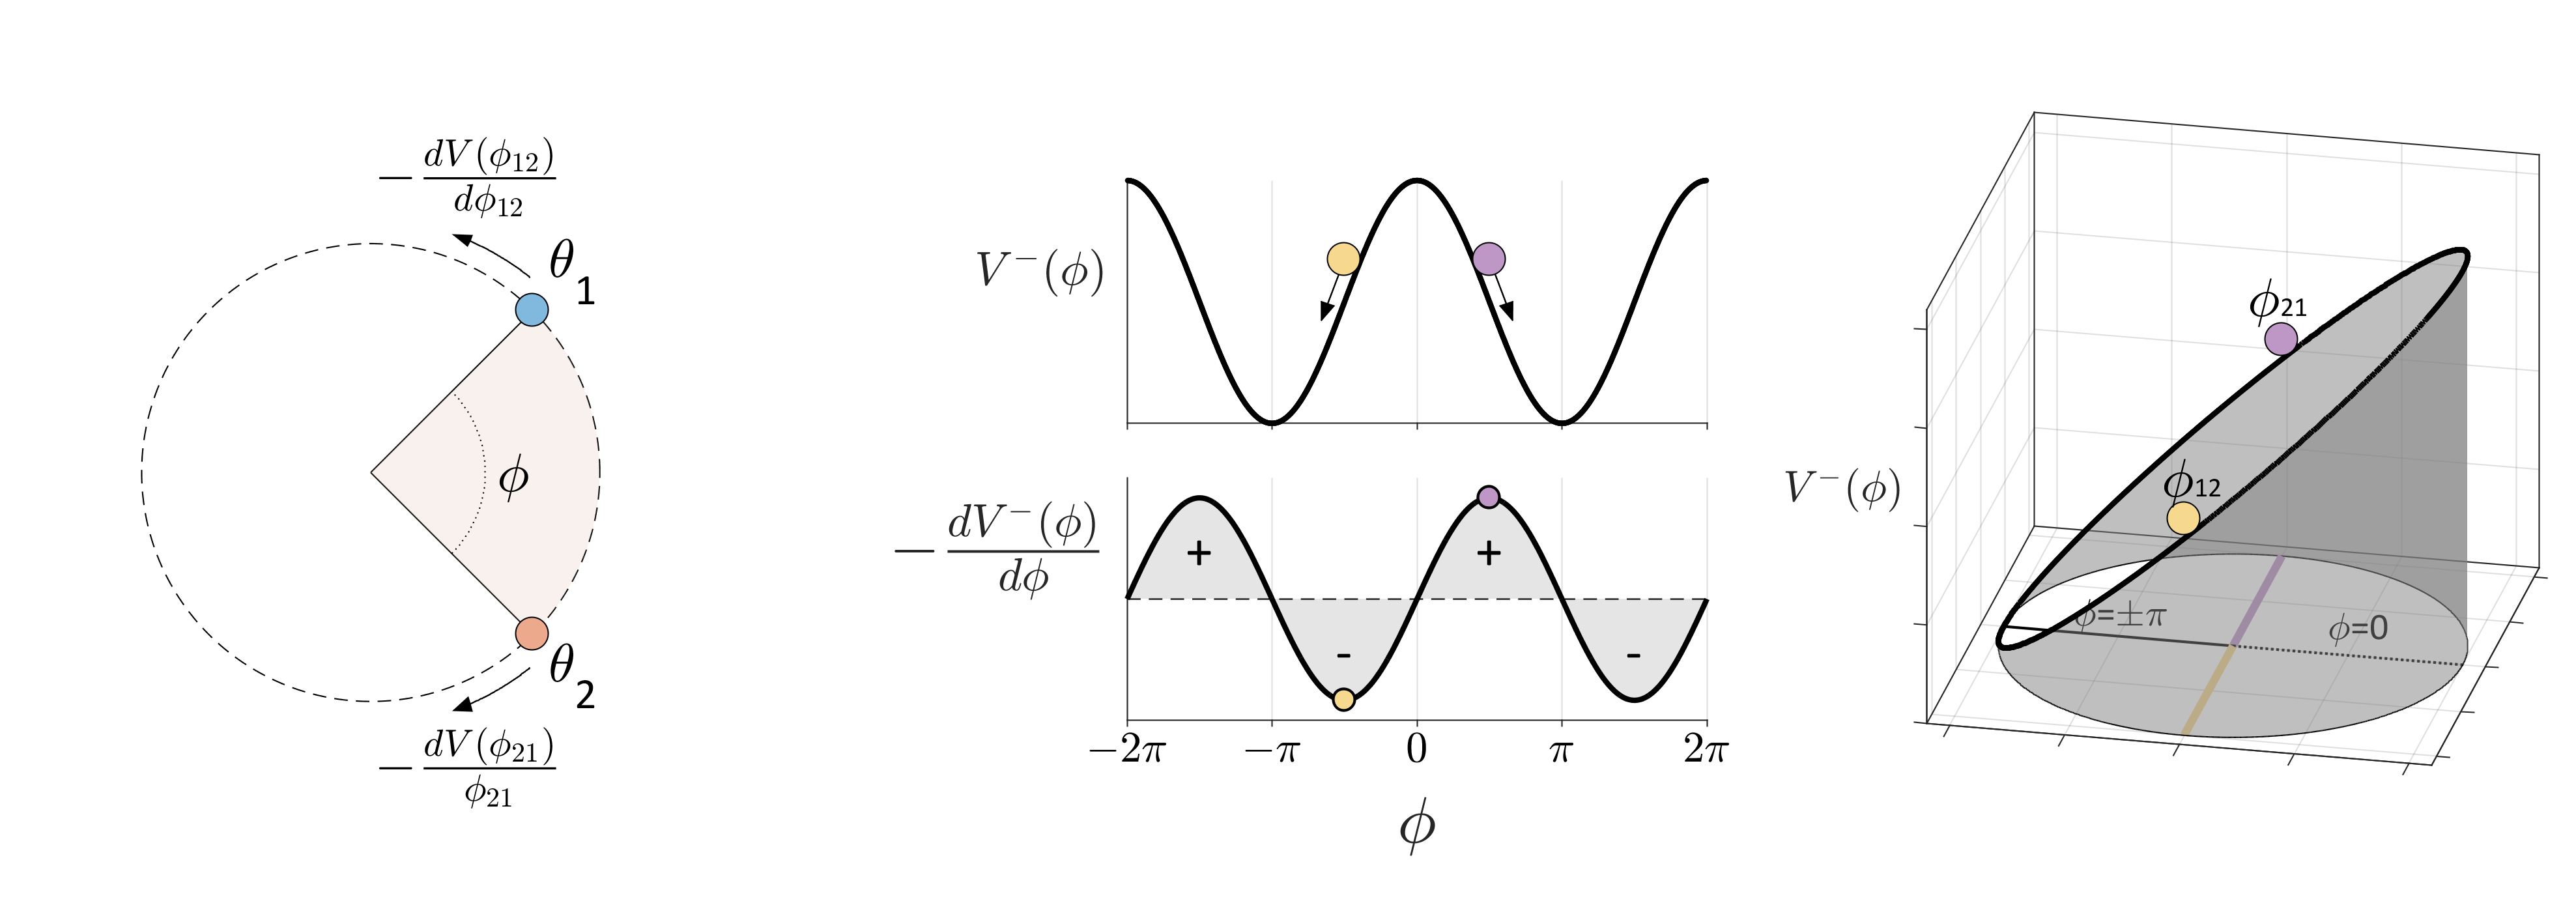
\includegraphics[width=\textwidth]{figures/Tilsen-img19.png}
\caption{\missingcaption}
\label{fig:}
\end{figure}
 

  The other type of force is excitation coupling (e-coupling). Excitation coupling is an interaction which depends on and influences \textit{e} variables. An excitatory e-coupling force results in each system increasing the \textit{e} value of the other, and an inhibitory e-coupling force results in the each system decreasing the \textit{e} value of the other. We do not specify a functional form for this force, as its role in the current framework is not well developed and is generally secondary to other mechanisms.

  Both φ-coupling and e-coupling forces can have positive [+] or negative [-] valence, as schematized below. An attractive (+φ) force causes the θ of systems to become more proximal and a repulsive (-φ) force causes θ to become more distal. An excitatory (+e) force causes \textit{e} values to increase, and an inhibitory (-e) force causes \textit{e} values to decrease: 

  
\begin{figure}
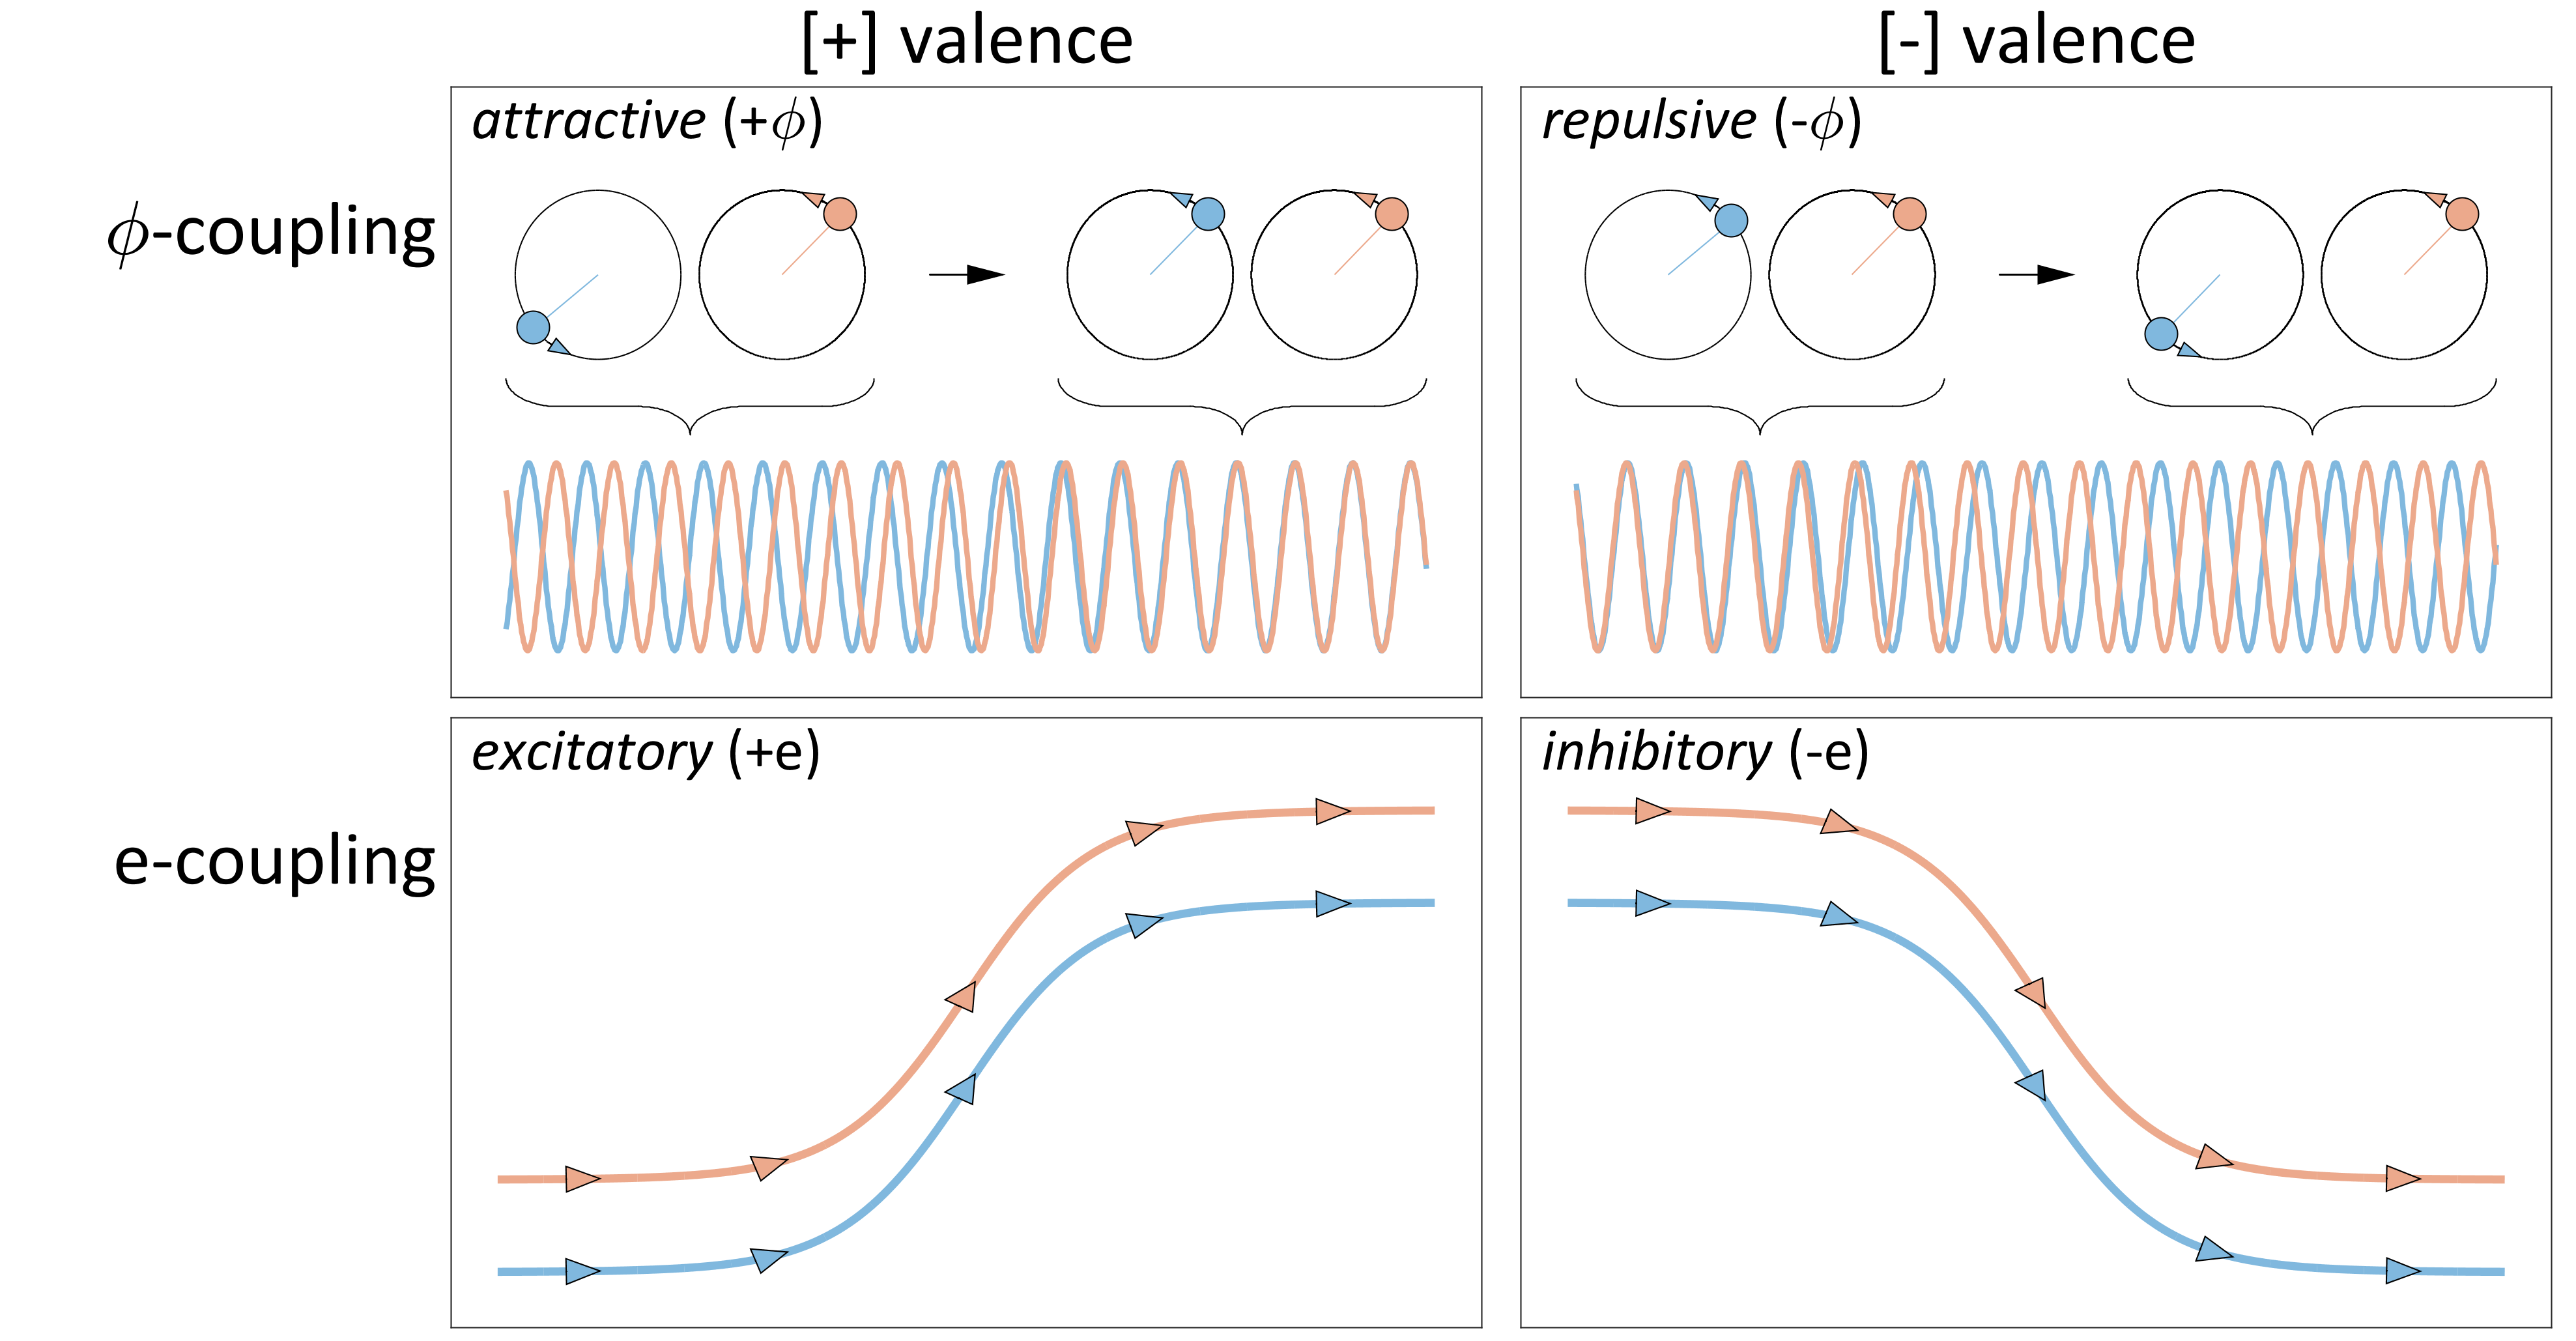
\includegraphics[width=\textwidth]{figures/Tilsen-img20.png}
\caption{\missingcaption}
\label{fig:}
\end{figure}
 

  The equations below show the roles of φ- and e-forces in influencing how θ and \textit{e} variables change in time. The total φ- and e-forces a system experiences are sums over forces from pairwise interactions with other systems, plus forces from the surroundings, \textit{S}. These forces have coupling strengths/susceptibilities φ and $\varepsilon $, respectively. The φ-force from \textit{S} is negligible, because the surroundings are too large to exhibit a collective oscillation. However, the surroundings can exert non-negligible e-forces. The term \textit{f} is an intrinsic frequency of the system (angular velocity \textit{ω} = 2π\textit{f}), representing population-internal forces which promote collective oscillation. The operator  $\widehat {{E}}\left[\overrightarrow{{\theta} },\overrightarrow{{e}}\right]$ is a placeholder for mechanisms of e-organization, and we develop these in detail later on.

\begin{equation*}
{\acute{{\theta} }}_{i}={2\mathit{\pi f}}_{i}+{F}_{\mathit{\varphi S}}\left(S,{\theta} _{i}\right)+\sum _{j}{{{\Phi} _{\mathit{ij}}F}_{\varphi} \left({\varphi} _{\mathit{ij}},{e}_{i},{e}_{j}\right)}
\end{equation*}
\begin{equation*}
{\acute{{e}}}_{i}=\text{Ê}\left[\overrightarrow{{\theta} },\overrightarrow{{e}}\right]+{F}_{\mathit{eS}}\left(S,{e}_{i}\right)+\sum _{j}{{{\varepsilon} _{\mathit{ij}}F}_{e}\left({\varphi} _{\mathit{ij}},{e}_{i},{e}_{j}\right)}
\end{equation*}

  Some properties of φ- and e-coupling can be derived from our microscale conceptualization. For one, the valences of φ- and e-forces (i.e. the signs of elements of matrices φ and $\varepsilon $) are correlated: attractive and mutually excitatory coupling tend to co-occur, and repulsive and mutually inhibitory coupling tend to co-occur. The basis for this correlation is the association of [+] valence forces with predominantly excitatory post-synaptic targets of interpopulation synapses, and conversely the association of [-] valence forces with predominantly inhibitory neurons as post-synaptic targets. These microscale patterns are illustrated below. When the excitatory neurons in population A project primarily to excitatory neurons in population B, the effect of spikes of those neurons is to attract θ\textsubscript{B} to θ\textsubscript{A} and augment \textit{e}\textsubscript{B}; when excitatory neurons in B project primarily to inhibitory neurons in B, their effect is to repel θ\textsubscript{B} from θ\textsubscript{A} and diminish \textit{e}\textsubscript{B}. 

  
\begin{figure}
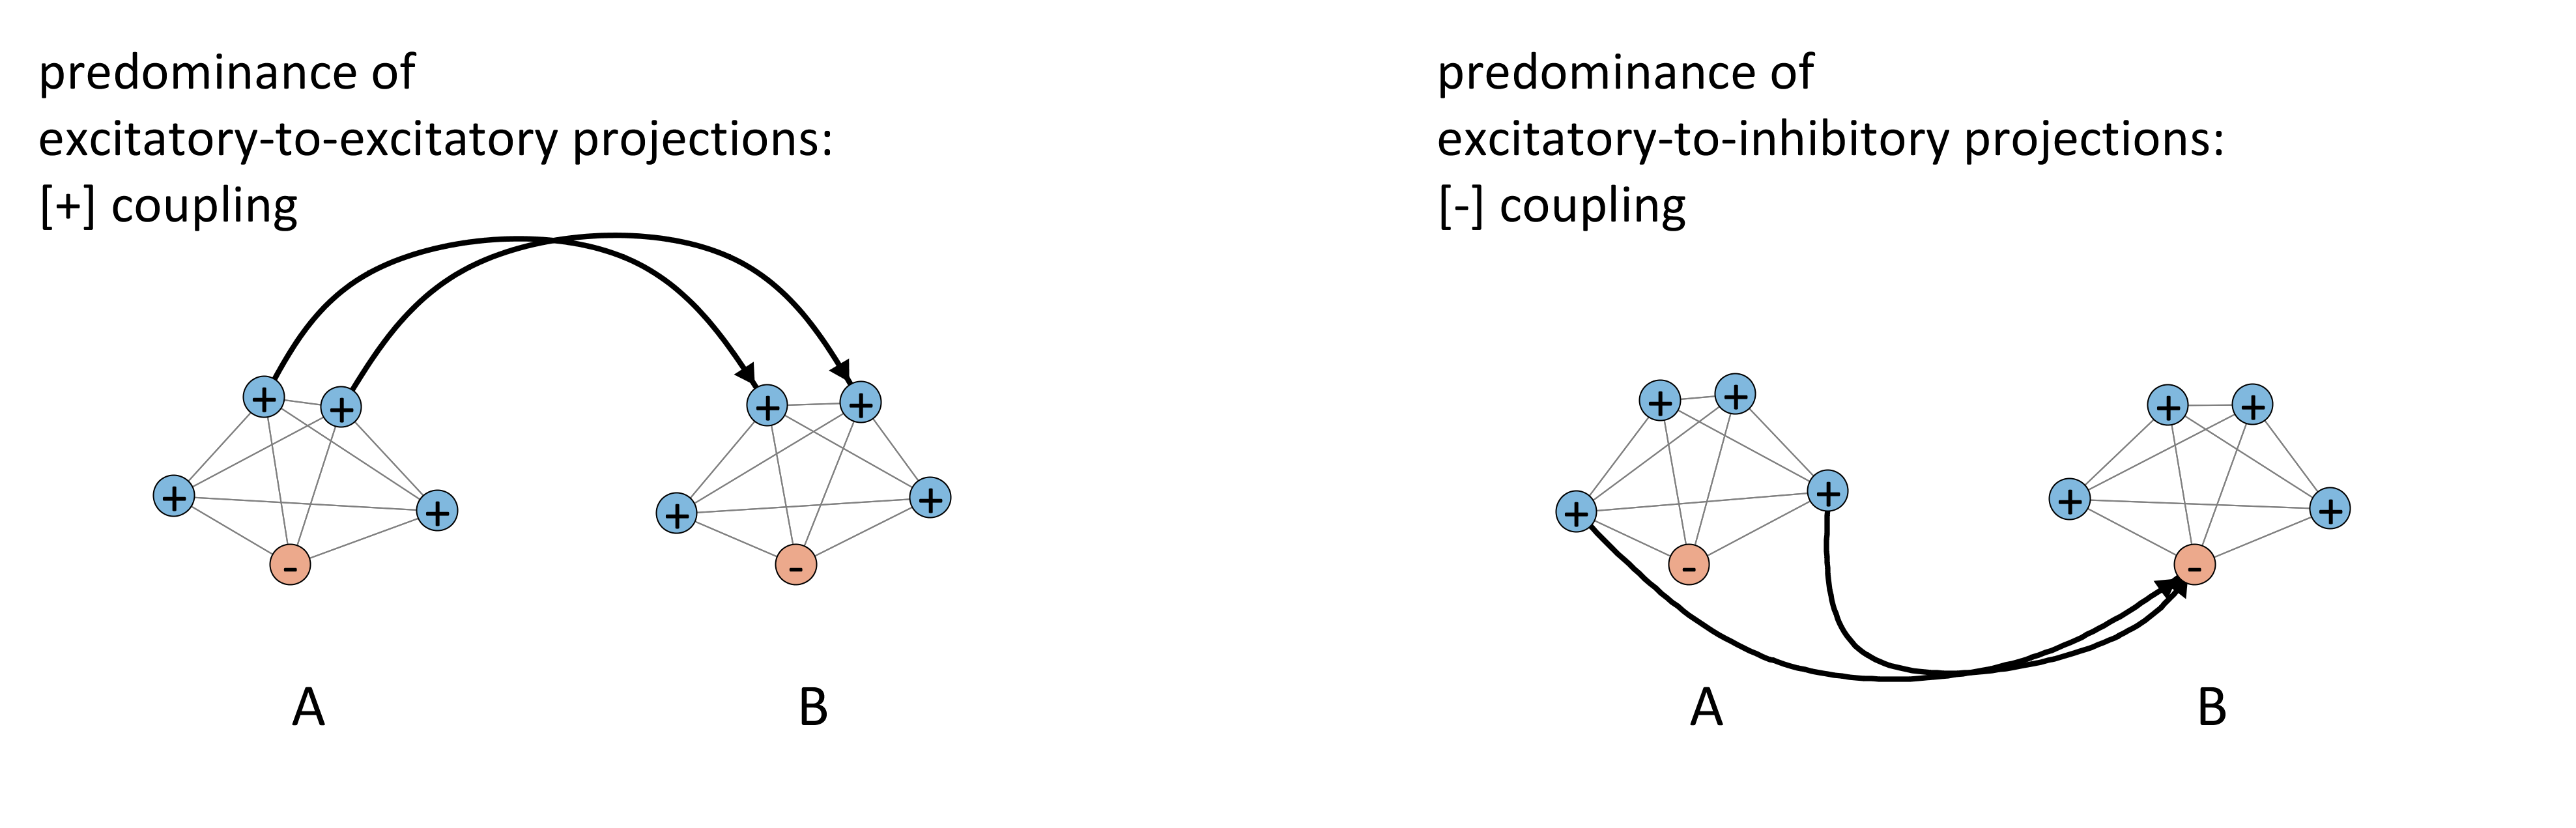
\includegraphics[width=\textwidth]{figures/Tilsen-img21.png}
\caption{\missingcaption}
\label{fig:}
\end{figure}
 

  The correlation of φ and $\varepsilon $ and valence implies that φ- and e-forces depend on both φ and \textit{e} values of systems. However, we offer no specific form for the φ-e interaction here because it would be too speculative. Nonetheless, our hypothesis that relational meaning experiences require the relevant cs-systems to be in an excited state can be viewed as a hypothesis that φ-coupling forces are modulated by \textit{e} values: the φ-forces exerted by unexcited systems are too weak to stabilize φ configurations, while systems with above-threshold \textit{e} values can exert φ-forces on one another that are sufficiently strong to induce a high degree of cs-system coherence.

  The φ- and e-coupling force matrices φ and $\varepsilon $ are also sign-symmetric. The basis for this is that Hebbian learning between bidirectionally coupled populations would be unstable on long timescales, if the valences of interactions between those populations were asymmetric. For instance, imagine a population A that is +φ coupled to population B, while B is -φ coupled to A. Spike-timing dependent learning would strengthen synapses which promote attraction of θ\textsubscript{B} to θ\textsubscript{A}, but also strengthen synapses which promote repulsion of θ\textsubscript{A} from θ\textsubscript{B}, leading to an unstable interaction in which A chases B while B runs away. Thus valence-symmetry is expected for a pair of systems. In contrast, there is no reason to expect a high degree of correlation in pairwise coupling strength for either φ- or e-coupling forces. These strengths are derived from numbers of synapses (or synaptic density, i.e. average number of synapses per neuron). To summarize, the elements of φ are correlated in sign and magnitude with those of $\varepsilon $, and within each matrix there is sign symmetry but not a high degree of correlation.

\subsection{The syntactic mechanism for organizing relational meaning}

With the conceptual tools outlined above we can construct a new understanding of the flexible emergence of relational meaning experiences. The key idea is that stable, invariant φ configurations between c-systems are created indirectly through their cs-resonances with strongly coupled s-systems. The coupling structure and phase circle representations for two example configurations are schematized below. The [Al][drinks] +φ configuration obtains because the c-system [Al] resonates with the s-system \{+N\}, the c-system [drinks] resonates with the s-system \{V\}, and the s-systems \{+N\} and \{V\} are strongly +φ coupled. Likewise, [coffee] resonates with \{-N\}, and \{V\} and \{-N\} are strongly -φ coupled.

  Although φ configurations can be decomposed into pairwise relations, multiple φ configurations which obtain simultaneously will often be shown by projecting them onto the same relative phase axis, as below. Furthermore, because the hypothesized mechanism for stabilizing φ configurations is strong φ-coupling between s-systems, the phase circle representation generally implies coupling between s-systems only; φ configurations between c-systems are an indirect consequence of strong s-system coupling. We nonetheless sometimes label c-systems on the phase circle for convenience. Because a φ configuration of c-systems entails the same configuration between the s-systems which resonate with those c-systems, we think of a φ configuration as a configuration of a cs-system. 

  
\begin{figure}
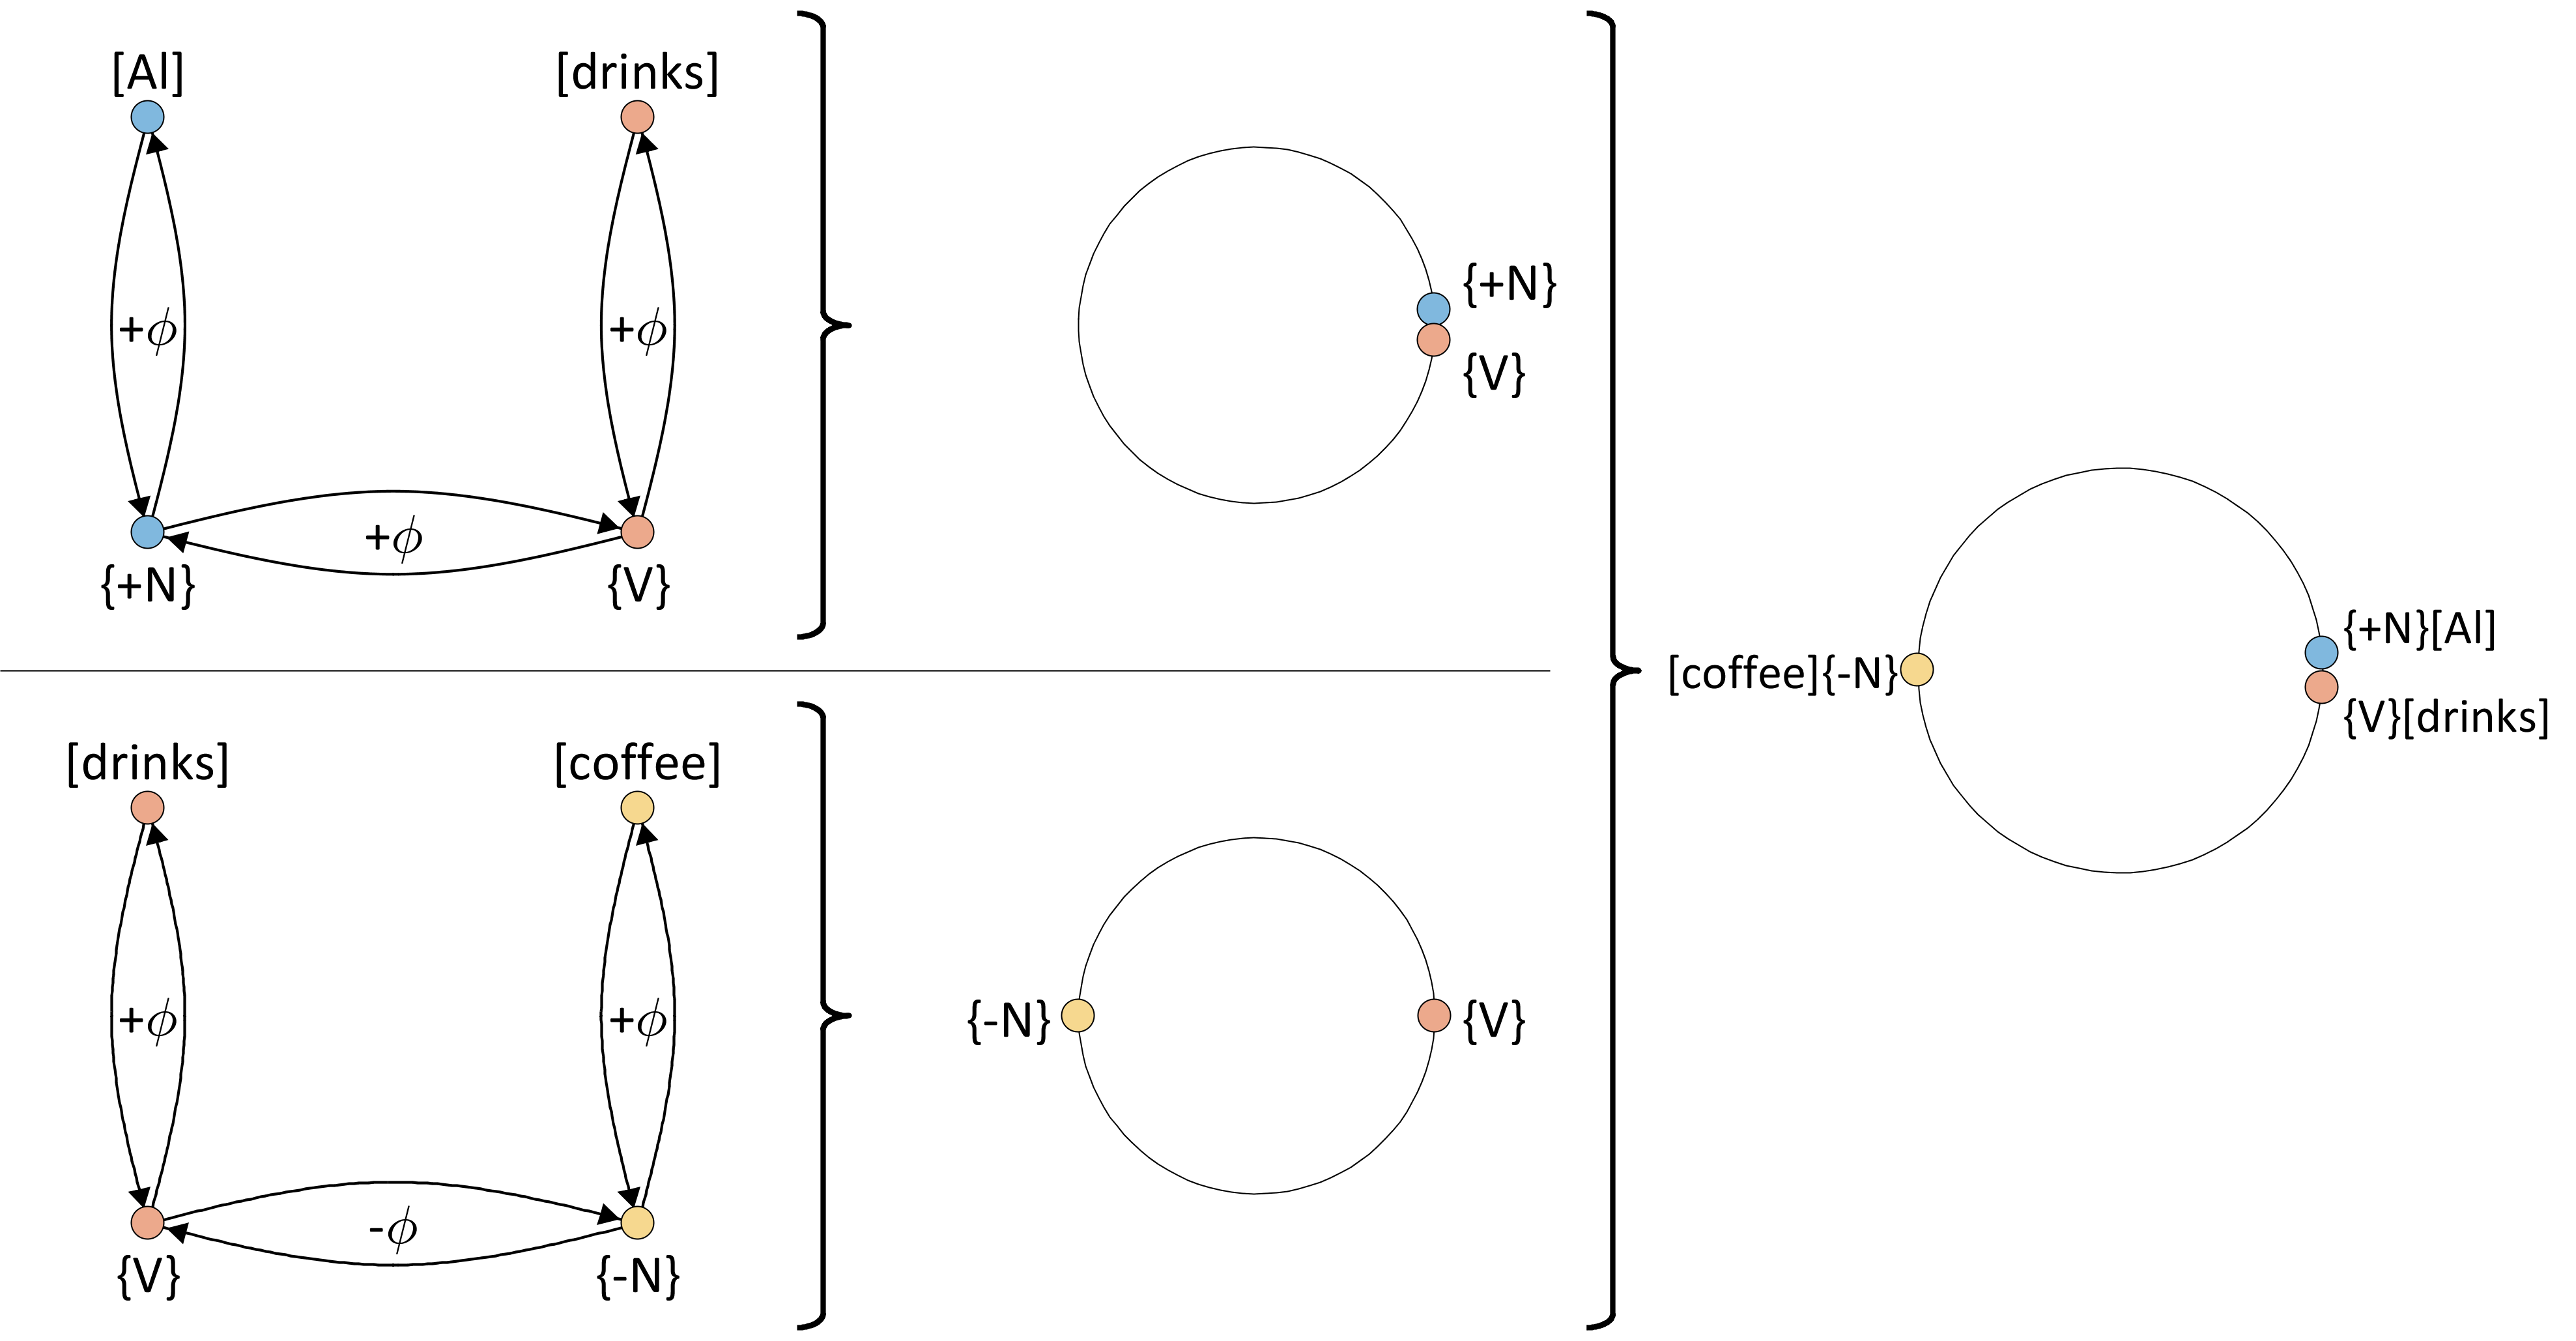
\includegraphics[width=\textwidth]{figures/Tilsen-img22.png}
\caption{\missingcaption}
\label{fig:}
\end{figure}
 

  Importantly, a φ pattern alone is not sufficient for a relational meaning experience. In addition, the pattern must be stationary in a local epoch of time. For a pattern to be stationary, there must be a stabilizing mechanism, and s-systems provide this mechanism. Recall the dynamic equation for θ. In general, the intrinsic frequencies \textit{f}\textsubscript{i} of any two systems are not the same and fluctuations in surroundings forces constantly perturb their phase velocities θ\textsubscript{i}′. In the absence of coupling forces, intrinsic frequency differences and surroundings perturbations cause φ to drift. In contrast, with the strong coupling of cs- resonances, c-system and s-system phase velocities θ\textsubscript{i}′ equalize to a compromise $\theta ′$, the value of which depends on the relative strengths of the forces and the intrinsic frequencies. This will hold as long as the coupling forces—which act to equalize phase velocity—are strong compared to the perturbing forces. Thus given sufficiently strong coupling forces, a φ configuration will remain stable.

\subsection{Interference and differentiation}

The preceding analyses distinguished between \{+N\} and \{-N\}. Why do we need to make this distinction, and how can it be understood on the microscale? The distinction between \{+N\} and \{-N\} systems (and on the microscale, \{+N\} and \{-N\} populations) is necessary because of \textit{interference}. Imagine that there is just a single, undifferentiated \{N\} population. For an utterance like \textit{Al drinks coffee}, both [Al] and [coffee] resonate with \{N\}, and [drinks] resonates with \{V\}. According to the relational meaning hypotheses presented earlier, [Al]\{N\} and [coffee]\{N\} should obtain +φ and -φ configurations with [drinks]\{V\}, respectively. These conditions are incompatible: it is not stable for \{N\} to be simultaneously +φ and -φ coupled to \{V\}.

  How does the nervous system resolve this dilemma? A crucial constraint on any solution is that populations cannot be created or added (cf. the multiplicity problem). We cannot simply posit that there is a second \{N\} population, independent of the original one. Instead, we imagine that there is one single \{N\} population, and that speakers learn to differentiate that population into \{+N\} and \{-N\} subpopulations, which are biased to +φ and -φ couple to \{V\}, respectively.

  A consequence of the differentiation mechanism is that subpopulations can \textit{interfere} with one another and become unstable. This can happen for two reasons. First, when a population is differentiated, the resulting subpopulations are smaller than the original population. The interaction forces exerted by the subpopulations on other systems become smaller, and the subpopulations themselves become more susceptible to forces from other systems and the surroundings. This can ultimately result in instability. Second, differentiated systems are not entirely independent: the corresponding subpopulations will typically overlap. The repeated differentiation of a finite population eventually results in instability, because the resulting subpopulations become smaller and have greater degrees of proportional overlap. The \{N\} > \{+N\}/\{-N\} differentiation provides two \{N\} populations which are quite stable when simultaneously excited, but when we differentiate one of these subpopulations further, stability may be threatened. The loss of stability from differentiation has important consequences which we examine in later chapters.

\section{Selection and quantal organization of excitation}

Whereas the principle of relational meaning involves organization of relative phase (φ), the principle of quantal excitation involves organization of excitation (\textit{e}). The movements associated with the production of speech arise from an organized, ordered selection of systems, determined by their relative excitation. Selection is a mechanism in which supra-threshold excitation of systems induces excitation of gestural/motor systems. Here we propose \textit{a principle of quantal excitation}: syntactic systems are organized and re-organized in a quantal relative excitation potential. This organization results in the ordered selection of motor behaviors associated with language.

\subsection{A quantal relative excitation potential}

The principle of quantal excitation is based on a conjecture that there exists a mechanism which organizes the relative excitation of s-systems into quasi-discrete, or \textit{quantal} excitation levels. We identify this mechanism with a \textit{stabilizing regime} of the excitation operator Ê in the dynamical equation for \textit{e}. The stabilizing regime of Ê is one in which \textit{e} states are mapped to themselves, and thus relative \textit{e} values remain constant. The stabilizing regime of Ê is associated with a conservative excitation potential, V(\textit{e}), as shown below for utterances \textit{Al sleeps} and \textit{Al drinks cold coffee}. 

  Observe in the examples that there are large differences in potential energy between excitation levels. The potential barriers between excitation levels entail forces which stabilize s-system \textit{e}, thereby preventing \textit{e} values from increasing to a higher level. The force that each system experiences is –dV(\textit{e})/d\textit{e}, i.e. the opposite of the derivative of the potential. The conception of force and potential energy here derives from an analogy to conservative forces, but we do not actually require a conserved quantity. Furthermore, we imagine these forces to be stationary for only for a local period of time, i.e. a single epoch of e-organization during which Ê is in the stabilizing regime. 

  
\begin{figure}
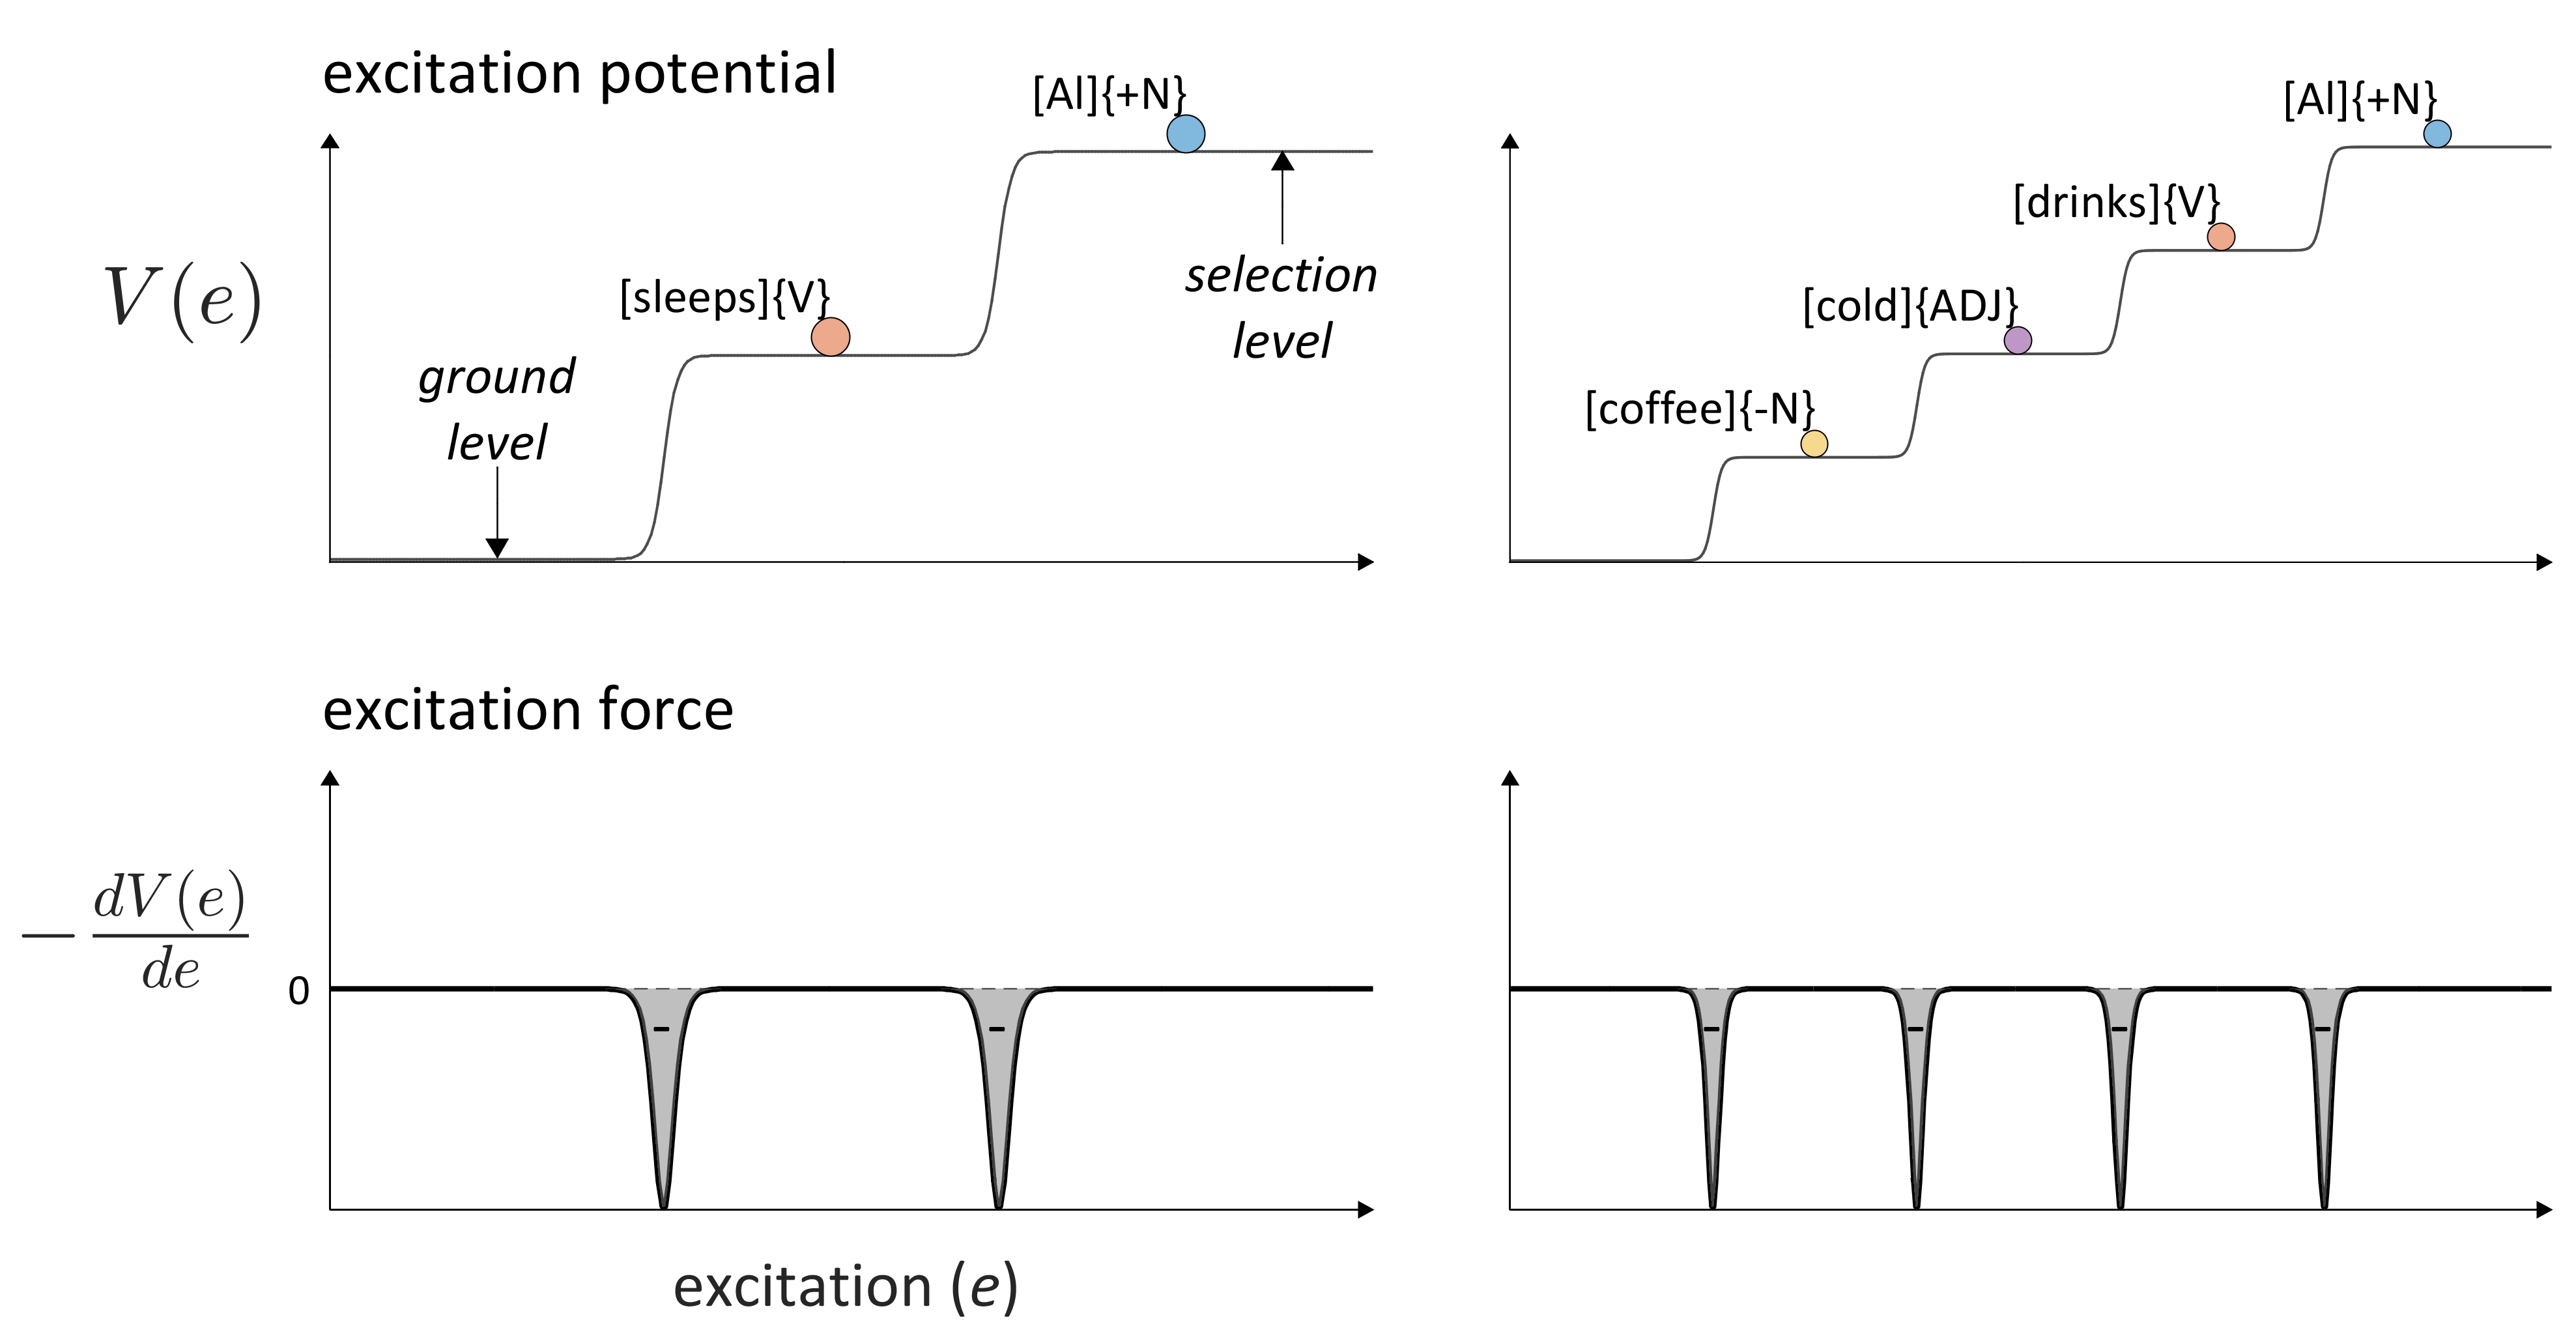
\includegraphics[width=\textwidth]{figures/Tilsen-img23.png}
\caption{\missingcaption}
\label{fig:}
\end{figure}
 

  Two levels of the potential representation have a special  interpretation. The lowest level of the potential is the \textit{ground level}, and systems on this level are by definition in an active, unexcited state. Ground state systems have at least the minimal \textit{e} value required for collective oscillation, but do not have sufficient \textit{e} to participate in a stable φ configuration. There are no “systems” below the ground level, because a system by definition is a population which exhibits collective oscillation. We distinguish \textit{ground level} systems from \textit{excited} systems, which have sufficient excitation to participate in stable φ configurations. The highest level of the potential is called the \textit{selection level}, and systems on this level have sufficient excitation to induce the selection of gestural/motor systems which are associated with a c-system. To summarize, there are three thresholds and four classes of excitation states:

\begin{table}
\begin{tabularx}{\textwidth}{llQ}
\lsptoprule
\textbf{level} & \textbf{state} & \textbf{description}\\
\midrule 
& inactive & system is undefined, no collective oscillation\\
\raggedleft ground-level & active,

non-excited & collective oscillation and minimal cs-resonance, 

\textit{e} insufficient for stable φ configuration\\
\raggedleft excitation levels & excited,

sub-selection & strong cs-resonance

\textit{e} sufficient for stable φ configuration\\
\raggedleft selection-level & selected & gates open for simulation or execution 

of associated gestural/motor systems\\
\lspbottomrule
\end{tabularx}
\caption{\missingcaption}\label{tab:key:}
\end{table}
 
 We have not addressed the question of how the quantal character of the relative excitation potential can be derived from a microscale model. Presumably, quantal e-organization manifests partly from e-coupling interactions between s-systems, and we note that the effects of the potential are reminiscent of normalization mechanisms associated with on-center/off-surround fields \citep{Grossberg1978,Grossberg1987}. However, a detailed understanding of this mechanism has not yet been developed, and the quantal potential must currently be viewed as a phenomenological approximation with primarily heuristic value. Because of this, there is no reason to commit to a particular shape of the potential, and one can imagine a number of alternatives, as below:

  
\begin{figure}
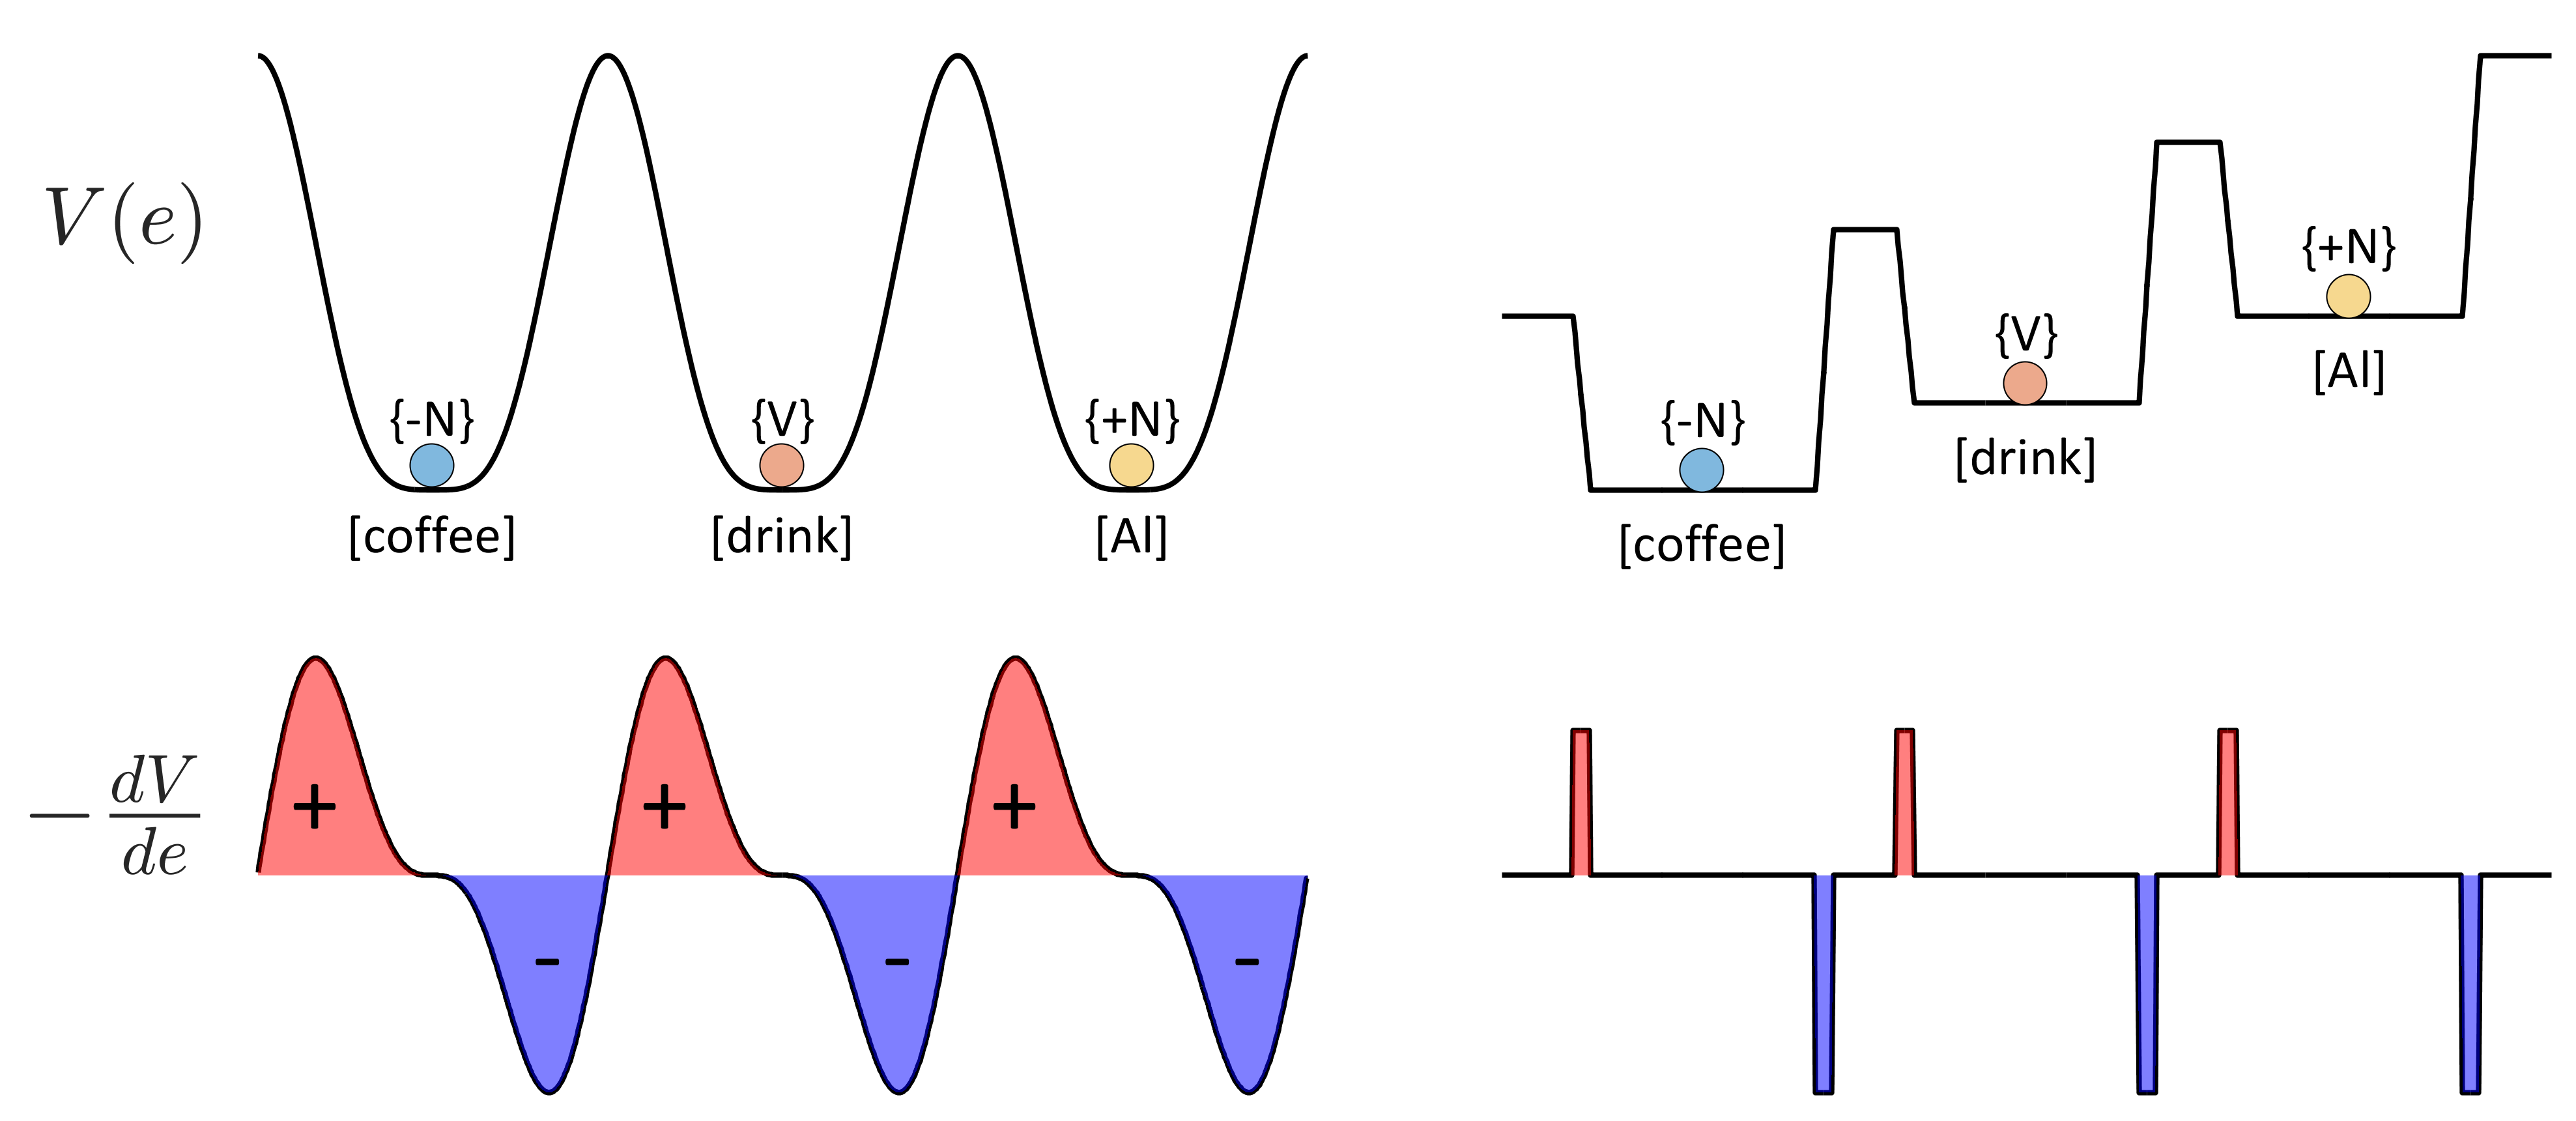
\includegraphics[width=\textwidth]{figures/Tilsen-img24.png}
\caption{\missingcaption}
\label{fig:}
\end{figure}
 

  Although the particular form of the potential function is not so important, its quantal nature is paramount, because the effect of the potential must be to stabilize a pattern of relative excitation which enforces mutual exclusivity of selection. Hence, when [Al]\{+N\} is selected, [drink]\{V\} and [coffee]\{-N\} are not selected, and so on. 

  There are several points to emphasize regarding the e-potential representations. First, as explained above, these representations are schematic and imply discretized patterns of relative excitation; they do not imply specific values or specific relative magnitudes. Second, e-potentials govern the \textit{e} values of s-systems, not c-systems. In cs-resonances, c-system \textit{e} values are correlated with s-system \textit{e} values, but the correlation is not exact. We nonetheless often label c-systems in e-potentials, for convenience, and often refer to cs-systems in this context. 

  Third, intermediate levels of an e-potential \textit{never exist independently of the systems which occupy them}. The potential is conceptualized as an emergent phenomenon associated with interactions between s-systems, and as such it is not sensible to imagine an “unoccupied level”. (The ground and selection levels are exceptions, for reasons we discuss later.) The potential levels are \textit{not} locations in space, and the systems are \textit{not} objects which occupy locations. Instead, the quantal potential is understood as a pattern of organization that is created by a combination of local interactions between s-systems and a general purpose ordering mechanism which operates on an \textit{e} value code. Rather than saying that systems \textit{occupy} levels, it is more precise to say that interactions between s-systems bring about the conditions for the stabilization of their relative excitation.

\subsection{Canonical reorganization}

While the stabilizing regime of Ê enforces an approximate temporal invariance on \textit{e}, a reorganization regime of Ê causes intermittent, abrupt changes in \textit{e}. These changes map \textit{e} configurations to \textit{e} configurations in predictable ways. Reorganization mappings cause changes in \textit{e} configuration which are discontinuities on the φ-timescale. We refer to the stable periods of time between these discontinuities as e-epochs. We are interested here in the various forms that reorganization mappings can take, and in what aspects of the system state they might depend on. In general, reorganization operations could depend on all θ and \textit{e} variables of all active and excited systems—i.e. the full system state. However, we can infer that some information is typically not relevant to the mapping. 

  The default mechanism for ordering the selection of systems is the canonical reorganization mapping, Ê\textsuperscript{cr}. θ/φ information is irrelevant for canonical reorganization. The operation  can be understood as follows, using the utterance \textit{Al drinks coffee} as an example. First, assume the initial condition in epoch (e1), an \textit{e} configuration which is stabilized by stabilization regime Ê. In epoch (e1), [Al]\{N\} has selection-level excitation, and this drives the excitation of motoric/gestural systems associated with [Al]. Feedback resulting directly or indirectly from motoric/gestural excitation eventually causes a transition to the canonical reorganization regime. The canonical re-organization mapping Ê\textsuperscript{cr} causes an abrupt change from epoch (e1) to epoch (e2), in which the selection-level system is \textit{demoted} to the lowest excited state, and all other excited systems are promoted one level. Ê\textsuperscript{cr} applies to transitions from (e2) to (e3) and from (e3) to (e4) as well. Note that Ê\textsuperscript{cr} produces a cycle when iterated: e\textsubscript{1}, e\textsubscript{2}, … e\textsubscript{n}, e\textsubscript{1}… 

  
\begin{figure}
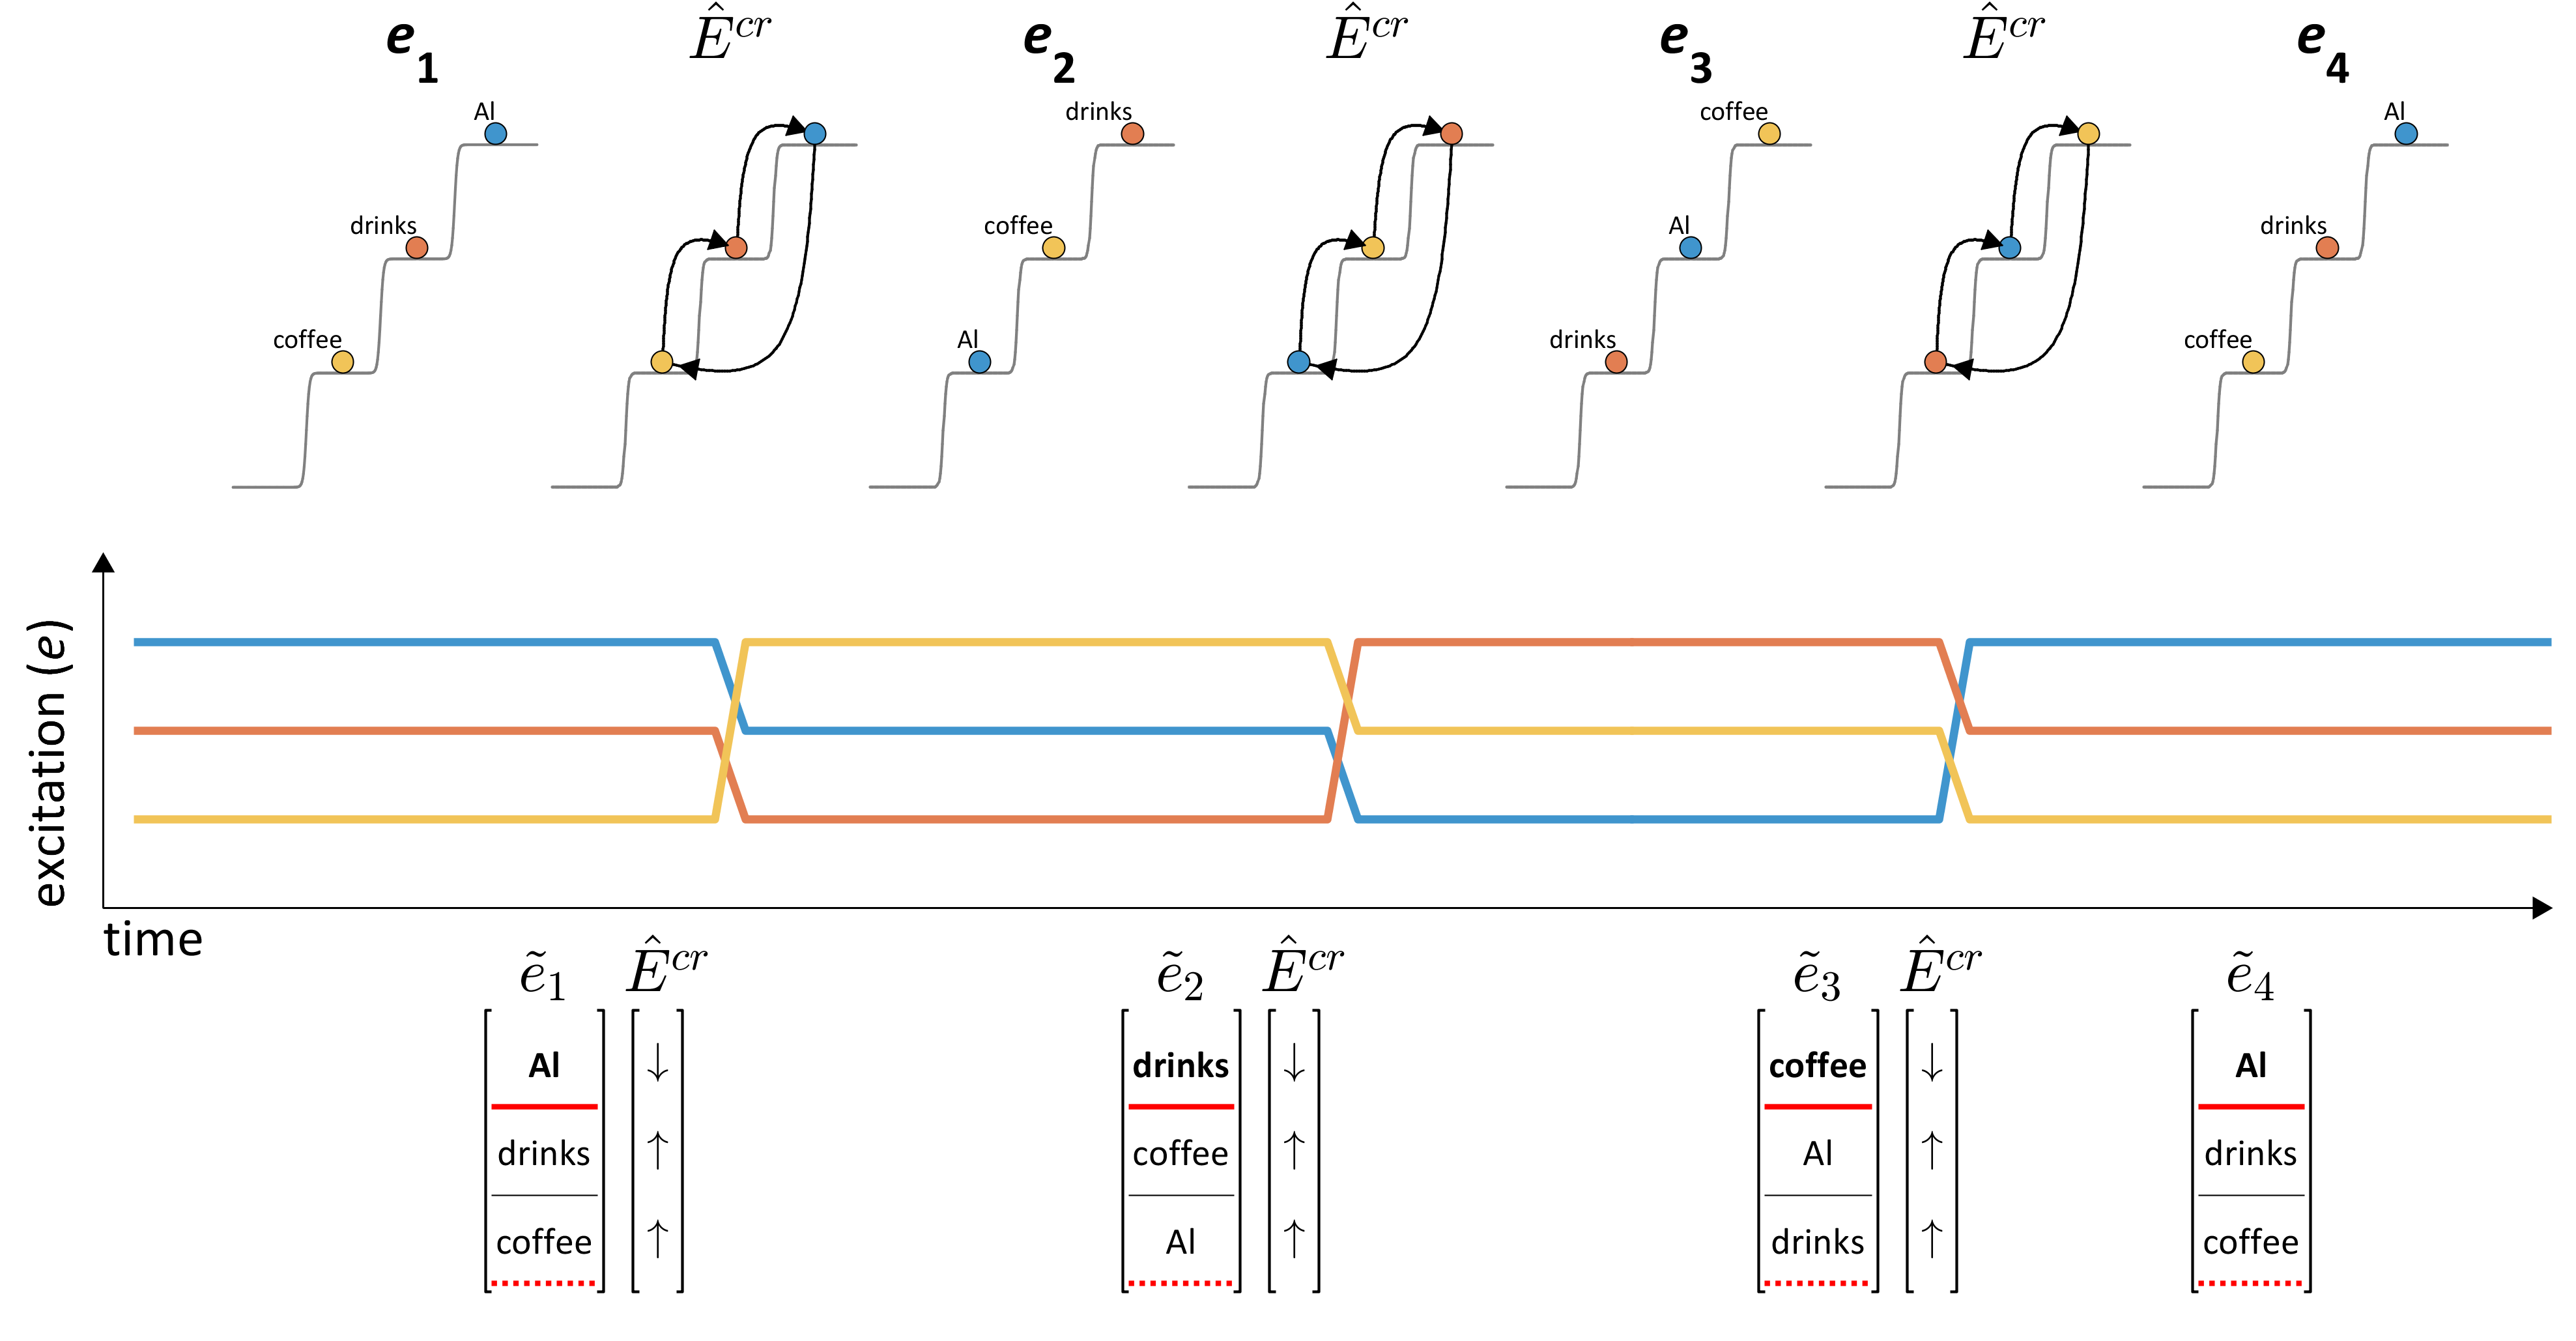
\includegraphics[width=\textwidth]{figures/Tilsen-img25.png}
\caption{\missingcaption}
\label{fig:}
\end{figure}
 

  Above we show a more compact representational formalism in which e-organization state vectors,  $\widetilde{{e}}$, are operated upon element-wise by reorganization vectors. In an e-organization state vector, systems are assigned to vector dimensions in order of their relative excitation. The figure above shows e-organization state vectors from a series of epochs. Each  $\widetilde{{e}}$ is operated upon by the canonical reorganization operator Ê\textsuperscript{cr}. The arrows in each element of Ê\textsuperscript{cr} indicate which basic operation (promotion or demotion) applies to the corresponding element of  $\widetilde{{e}}$. In this context, canonical reorganization can be understood as demotion of the most highly excited system to the lowest above-ground level, and promotion of all other systems by one level. For convenience, the excitation and selection thresholds are shown by dashed and solid red lines, respectively.

  There are a couple alternative formal approaches to representing reorganization mappings. One is to define a relative quantal excitation state vector  $\overrightarrow{{e}}$, where each dimension corresponds to a different excited cs-system. The value in a dimension is an integer from 1 to \textit{n}, where \textit{n} is the number of s-systems which occupy distinct e-levels, and the value corresponds to excitation rank order of the corresponding system. The canonical reorganization mapping in this scheme is shown below.

\begin{equation*}
{\text{Ê}}^{\mathit{cr}}\left(\overrightarrow{{e}}\right):e\rightarrow \left[e\mathit{mod}n\right]+1
\end{equation*}

  Another formalization uses a cyclic permutation matrix. In this case we define the e-state as a binary matrix Ë where each column corresponds to a level of the e-potential and each row to a system (so, a value of 1 in row \textit{n}, column \textit{m}, entails that system \textit{n} occupies excitation level \textit{m}). Repeated action of the permutation matrix Ê on Ë results in a return to the initial pattern. 

% \begin{equation*}
% \text{Ê}^{\mathit{cr}}=
% \left[
%   \begin{matrix}
%   0 & 0 & 1\\
%   1 & 0 & 0\\
%   0 & 1 & 0
%   \end{matrix}
% \right],
% {\text{Ë}}_{1}=
% \left[
%   \begin{matrix}
%   1 & 0 & 0\\
%   0 & 1 & 0\\
%   0 & 0 & 1
%   \end{matrix}
% \right]
% \end{equation*}
\todo{commented out matrix}


  The e-state vector and matrix representations are somewhat less general than the e-organization representation, for reasons that will become clear later. In contrast, the e-organization representation has greater flexibility and we make extensive use of it. The canonical reorganization is a useful construct because many of the phenomena we are interested in can be analyzed in relation to the canonical mapping.

  Although we do not attempt to model the internal dynamics of the reorganization process, we imagine promotion and demotion as brief periods of relatively strong excitatory and inhibitory forces. The picture we have in mind is below. In the stable epochs (e1) and (e2), the augmentation forces on [drinks]\{V\} and [coffee]\{N\} are not sufficient to promote these systems. But feedback regarding the selection of [Al]\{N\} induces a transition to the reorganization regime, in which there is a strong suppressive force on [Al]\{N\}, along with strong forces which augment the excitation of other systems. This may occur in combination with a reduction of the sizes of barriers in the potential. 

  
\begin{figure}
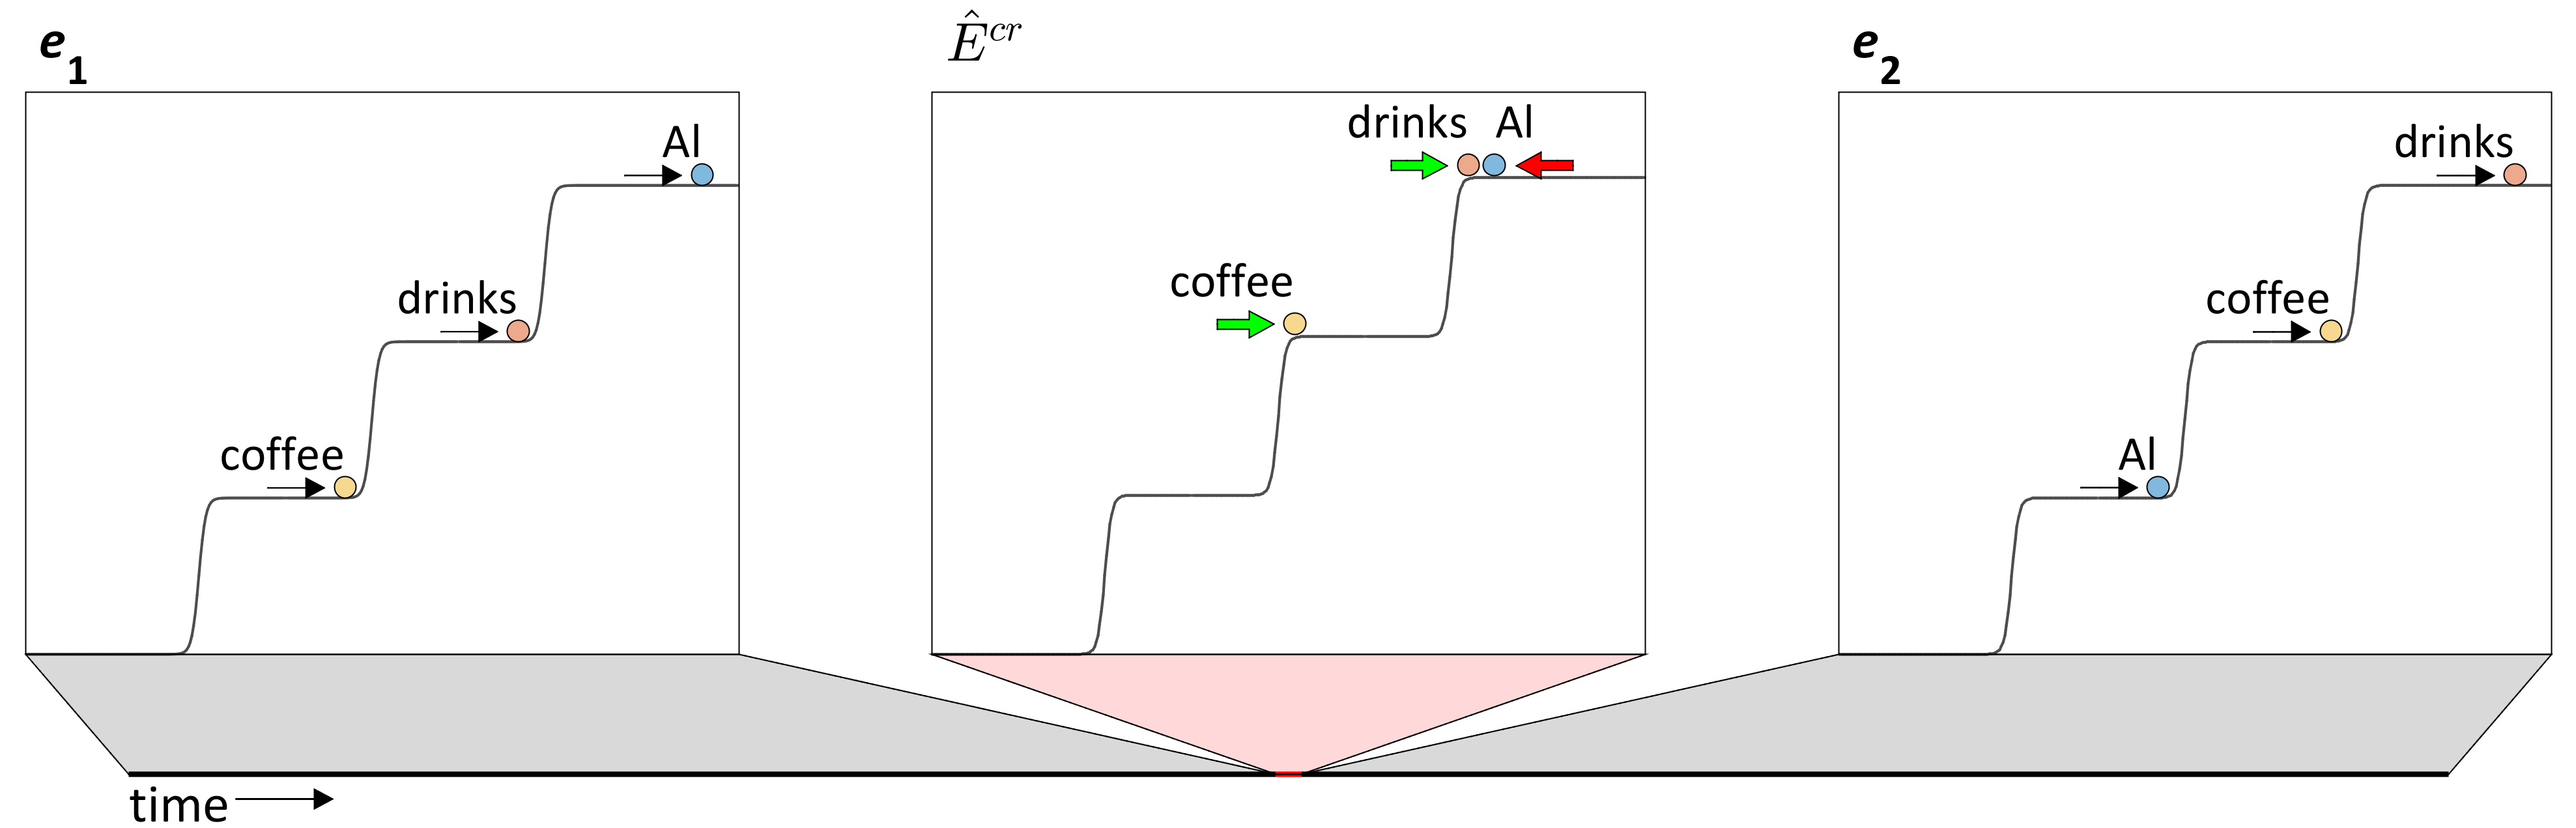
\includegraphics[width=\textwidth]{figures/Tilsen-img26.png}
\caption{\missingcaption}
\label{fig:}
\end{figure}
 

  The overall effect of the reorganization is that the \textit{e} value of the selected system, [Al]\{+N\}, decreases and the \textit{e} values of other excited systems, [drinks]\{V\} and [coffee]\{-N\}, increase. We assume that Ê returns to the stabilization regime when a new system surpasses a selection threshold, i.e. when [drinks]\{V\} is selected. It is important to emphasize that because systems are not objects, there is no sense in which there is a collision between objects. We never worry about lines crossing or objects occupying the same space in o/el representations.

\subsection{The combined picture: two conceptions of time}

The o/el framework provides two conceptual models of the temporality of speech, one which is suited for reasoning about relational meaning experiences, the other for action ordering. As shown below, a production trajectory begins with the activation of cs-systems. A stable φ configuration of excited systems then emerges in conjunction with an initial e configuration, as a result of an initial organization operator, Ê\textsuperscript{io}. (We examine mechanisms of initial organization in a subsequent chapter.) The \textit{e} configuration is then iteratively reorganized, while the φ configuration remains constant. Consequently, we see that φ-variables have a fixed point attractor throughout the trajectory (θ variables have a periodic attractor), while e-variables exhibit intermittent discontinuous changes. The steady state periods between reorganizations are e-epochs. The conceptual models of time we have constructed help distinguish between the φ-epoch timescale on which φ configurations are stable (i.e. a relational meaning experience is invariant) and the e-epoch timescale on which e configurations are stable.

  
\begin{figure}
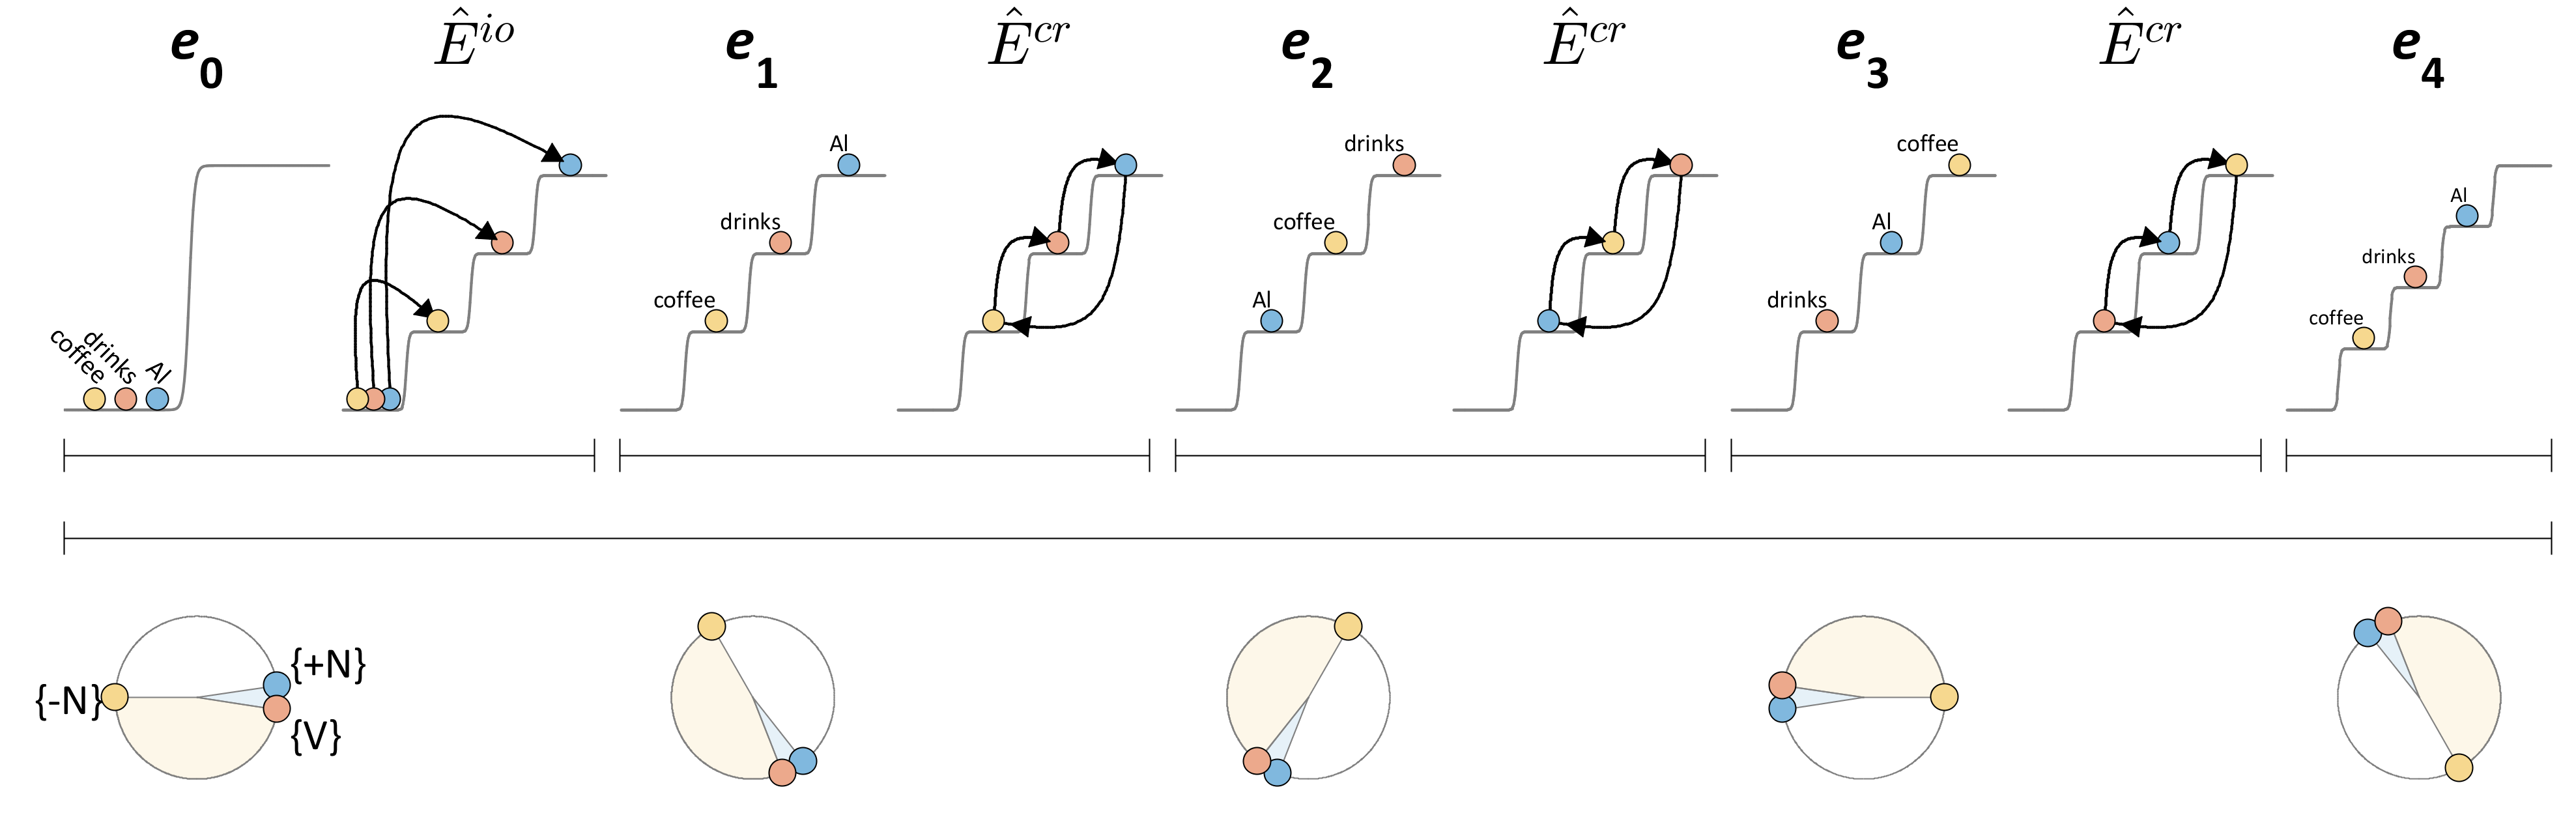
\includegraphics[width=\textwidth]{figures/Tilsen-img27.png}
\caption{\missingcaption}
\label{fig:}
\end{figure}
 

  In conventional approaches, there are diverse perspectives on how linearization (selection/ordering) and structure building (relational meaning) interact, but these are generally understood to create and operate on structures of connected objects. The o/el model provides an alternative framework for thinking about the interaction between relational meaning and temporal order, one specific to φ-organization, the other specific to e-organization. Because φ-epochs tend to span multiple e-epochs, it is not easy, nor even useful to combine them into a single space for visualization. One approach would be to map relative excitation to oscillator amplitude, in which case we can visualize the temporal evolution as below:

  
\begin{figure}
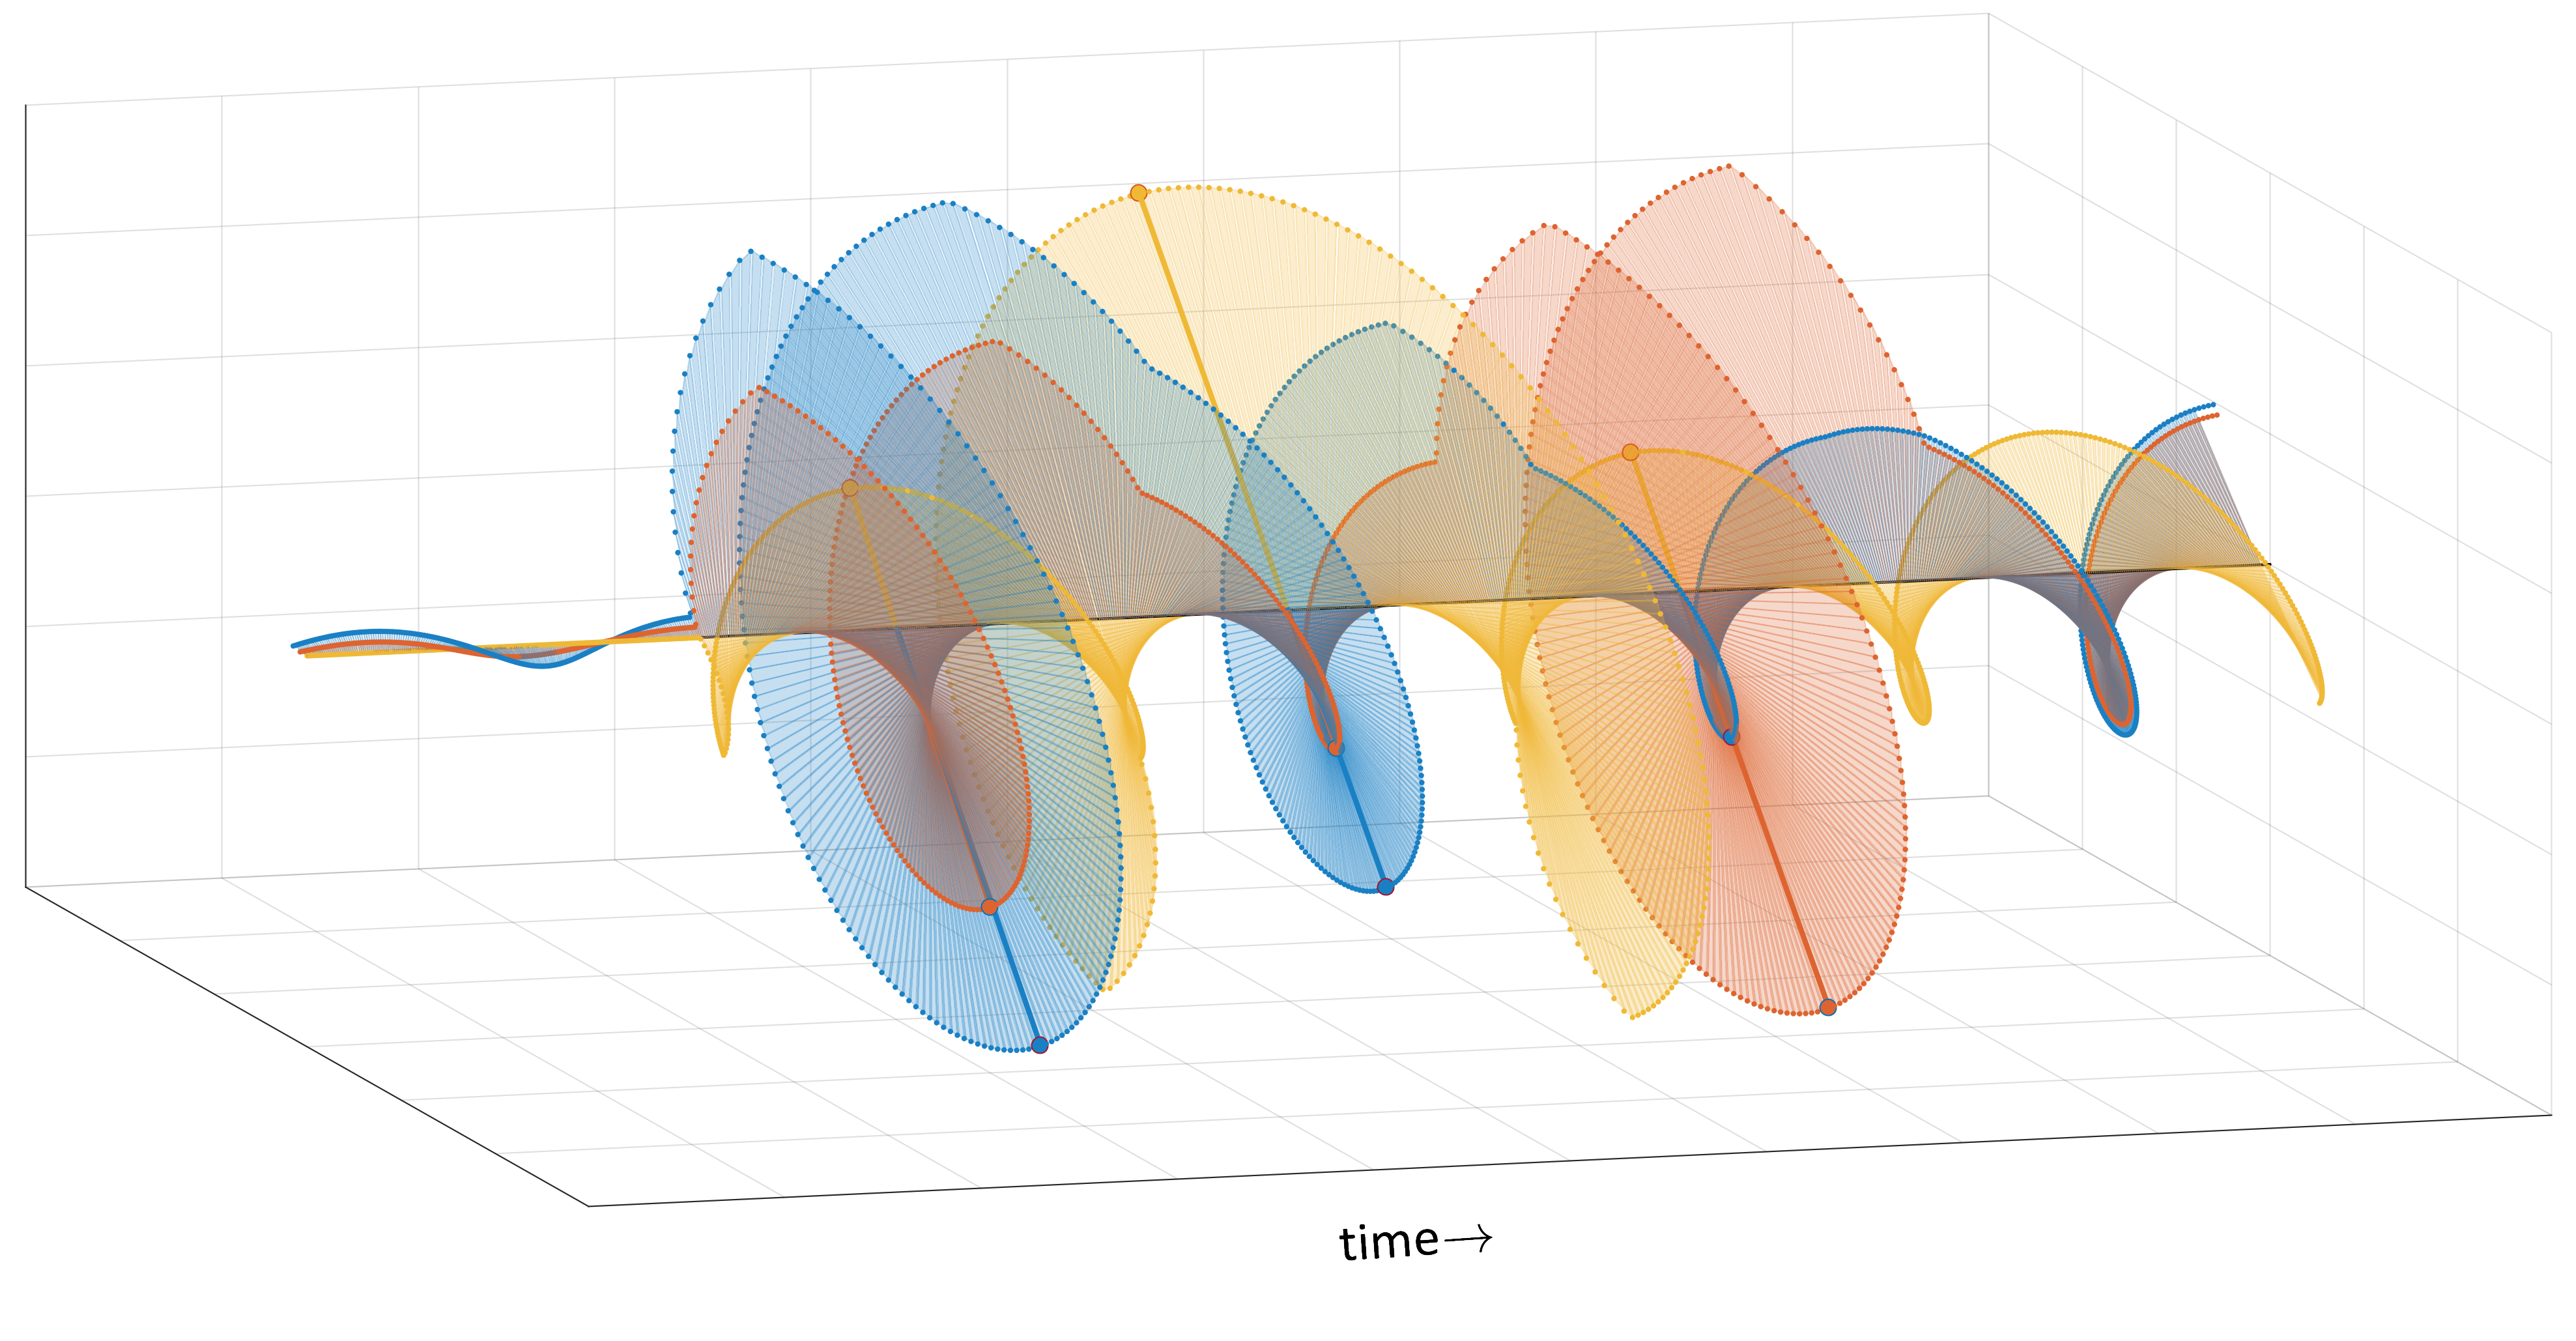
\includegraphics[width=\textwidth]{figures/Tilsen-img28.png}
\caption{\missingcaption}
\label{fig:}
\end{figure}
 

  This corkscrew visualization is too cluttered to be of much use, so instead we often juxtapose e-potential and φ{}-circle representations. These representations are analytical tools which encourage us to think differently about speech. Word order, instead of being a spatial arrangement of objects, is understood as a discontinuous trajectory in excitation space. Meaning relations, instead of being connections between objects, are experiences of stable relative phase differences between system oscillations.

\section{Conventions and terminology}

\textit{A}: order parameter of a system

\textit{S}: surroundings

θ, r: phase, radial amplitude of oscillatory component of order parameter
\textit{e}: excitation component of order parameter

φ: relative phase

c-system: concept system. written in square brackets, e.g. [coffee], [drink]

s-system: syntactic system. written in curly brackets, e.g. \{-N\}, \{V\}

cs-system or system: pair of resonating c- and s-systems, e.g. [drink]\{V\}, [coffee]\{-N\}

cs-systems in a stable configuration: {\textbar}drink coffee{\textbar}

Utterances: written italicized text, e.g. \textit{Al drinks coffee}

+φ-coupling/configuration: in-phase (attractive, proximal) relative phase-coupling/configuration

{}-φ-coupling/configuration: anti-phase (repulsive, distal) relative phase-coupling/configuration

+e-coupling: excitatory e-coupling

{}-e-coupling: inhibitory e-coupling

 $\widehat {{E}}$: e-organization operator
\chapter{Deconstructing syntactic theory}

All theories have deep assumptions, i.e. \textit{unknown} unknown knowns. These are the sorts of assumptions which are not questioned, and often cannot be questioned, because they are fundamental to a way of thinking and make an entire program possible. Often we are not aware of such assumptions. Yet by finding and rejecting these very well-hidden assumptions we can make progress toward new, different theories. To do this, we deconstruct the \textit{conceptual metaphors and image schemas}\footnote{There is a substantial literature in cognitive linguistics which formalizes and attempts to regularize notions of conceptual metaphor, image schemas, and blends. The deconstruction pursued here uses these notions informally and in an ad-hoc manner.} that are used to construct conventional syntactic theories. 

  A conceptual metaphor is a set of mappings from a more basic, experientially grounded source domain to a more abstract, conceptual target domain \citep{Lakoff1990,Lakoff1993,Lakoff2008,LakoffJohnson1980a,LakoffJohnson1980b,LakoffJohnson1999,LakoffJohnson200}). An image schema is a pattern generalized over sensory experience (mostly visual), and provides a source domain for conceptual metaphor (\citealt{ClausnerCroft1999,FauconnierTurner1996,FauconnierTurner2008,GibbsColston1995,GradyEtAl1999,Langacker2002,Oakley2007,Talmy1983,Talmy1988};. Theories are constructed by combining, or blending, conceptual metaphors and image schemas \citep{FauconnierTurner1996,FauconnierTurner2008,GradyEtAl1999,LakoffNúñez2000}. The art of theory construction (often a subconscious process) relies on intuitions regarding which metaphors/schemas to blend and which mappings to make use of.

  Many approaches to syntax\footnote{All approaches that I am aware of (present company excluded) are constructed from the delineated metaphors, but there may be other approaches I am not familiar with which are not. I am neither a historian of nor typologist of syntactic theories.}—an in particular generative/minimalist approaches—are constructed from the following set of conceptual metaphors: 

\begin{enumerate}
\item Linguistic units are objects.
\item Linguistic units are containers.
\item Relations between units are connections or containments.
\item Time is space.
\end{enumerate}

  Students of syntax are not taught these metaphors. They do not have to be, because they already know them. Generic versions of these metaphors pervade our conceptual models of abstract domains, and are learned at a fairly early age, especially in literate cultures. Also, there is no point in teaching students these metaphors (if we are even aware of them), because they are not on the table. Teaching them would allow them to be questioned, but they are for the most part non-negotiable. Even being consciously aware of them can be counterproductive, if one wants to participate in the normal discourse. For the lack of a better term, we consider syntactic theories/frameworks which presuppose these metaphors as \textit{conventional}, since it is currently a cultural convention to use these particular metaphors, as opposed to other ones. As mentioned in the introduction, I claim that generative/minimalist theories employ these metaphors, and I encourage the reader to assess their applicability to other theoretical frameworks.

\section{{The} {\textsc{units-}}{\textsc{are}}{\textsc{{}-objects}}{ metaphor}} 

In conventional models, “words” \textit{are} objects. Physical objects, of the sort you can hold. This is a metaphor, a set of mappings from a relatively concrete domain to a more abstract one. The abstract domain is language. The concrete domain is the domain of our experience with physical objects. Via the metaphor, our understanding of words is constructed from aspects of our experience with physical objects. It is not merely the \textit{use} of the word “object” that is crucial here. What is important is that our experience with physical objects is used to reason about metaphorical objects, “words”. For example, our experience with physical objects is such that we can join them together. This physical experience provides a basis for us to think of words as the sorts of things that can be joined together, or \textit{merged}, into larger structures.

  Literally, words are \textit{NOT} objects and are \textit{NOT} merged together in any physical sense. Indeed, “words” are very different from physical objects in many ways. We cannot literally touch words, hold them, join them together, or break them into pieces, etc. Nonetheless, we use the \textsc{words are objects} metaphor to construct a conceptual system for understanding “words”. Crucially, “words” do not exist independently of a conceptual system; rather, a conceptual system gives rise to a concept of a “word”. More generally, in the conventional program, \textsc{linguistic units are objects}: not only words but also phrases, sentences, etc. are objects. A number of mappings are associated with the objects metaphor. To see the importance of these mappings, consider the following descriptions of \textsc{Merge}: 

“The indispensable operation of a recursive system is Merge (or some variant of it), which takes two syntactic \textbf{\textit{objects}} α and β and forms the \textbf{\textit{new object}} γ = \{α, β\}.” \citep[3]{Chomsky2001}.

A natural requirement for efficient computation is a “no-\textbf{tampering} condition” NTC: Merge of X and Y leaves the two SOs \textbf{\textit{unchanged}}. If so, then Merge of X and Y can be taken to yield the set \{X, Y\}, the simplest possibility worth considering. Merge cannot \textbf{\textit{break up}} X or Y, or \textbf{\textit{add new features}} to them. \citep[5-6]{Chomsky2008}.

  Why does \textsc{Merge} “form” a \textit{new} thing? Why is the new thing also an \textit{object}? Why do merged objects not \textit{break up} or have new \textit{features added}? What does it mean for a syntactic object not to be \textit{tampered} with? The proclamations are comprehensible and make intuitive sense because they are consistent with our typical experiences in observing and interacting with physical objects. That is what makes conceptual metaphor so powerful: metaphor allows us to use our experiences with the familiar to construct an understanding of the unfamiliar. 

\subsection{Mappings of the object metaphor}

The conceptual foundations of conventional syntactic theories derive from mapping various aspects of our experiences with physical objects to the abstract domain of syntactic objects. A number of these mappings are catalogued below\footnote{This is neither an exhaustive list nor an essentialist construal of \textit{the} mappings of conventional theories, but rather one possible description of some of the more important ones.} .

  
\begin{figure}
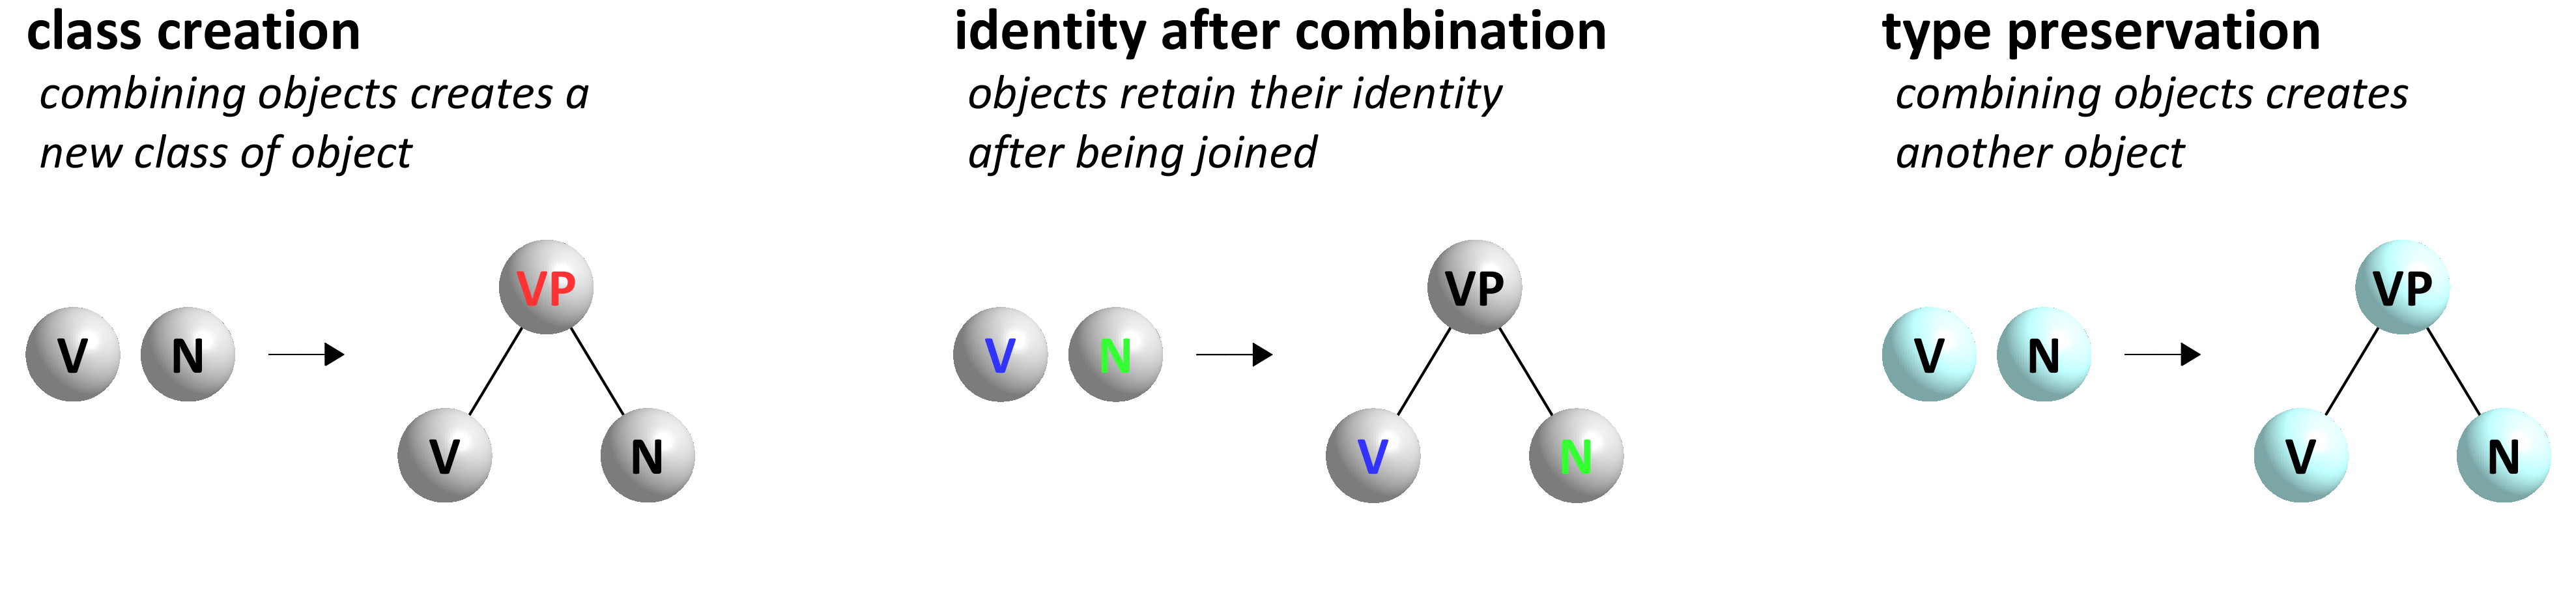
\includegraphics[width=\textwidth]{figures/Tilsen-img29.png}
\caption{\missingcaption}
\label{fig:}
\end{figure}
 

\textit{Class creation}: combining objects can create a new type of object. When we join a stick and a wedge-shaped stone we “create” an arrow. Likewise, when syntactic objects are combined, a new class of entity is created: word objects are combined to create phrase objects, and phrase objects are combined to create sentence objects. 

\textit{Identity preservation after combination:} the identities of the combined parts are retained after their combination. We can recognize the stick and wedge as continuing to be a stick and wedge after we have joined them, despite the fact that combining them creates a new object, an arrow. Likewise, when syntactic objects are combined, they retain their original identities.

\textit{Preservation of type:} the combination of things of a given type results in another thing of the same type. When we join physical objects, the joined entity is still a physical object. Likewise, the structures which are the inputs of merge are syntactic objects, and the structures which are the output of merge are syntactic objects.

  Mappings of the sort above are profoundly important for theory construction. They are intuitively sensible because they are based on typical experiences, rather than physical principles. Most of the mappings can be violated by considering atypical circumstances (quantum-scale phenomena, far-from-equilibrium chemical reactions, relativistic velocities, etc.). What matters is that in everyday situations, when we join objects together, it creates a new class of object, but we can usually continue to identify the component objects that were joined, and the new class of object is still the same type of thing, i.e. an object. There are many more mappings which come into play, for example:

  
\begin{figure}
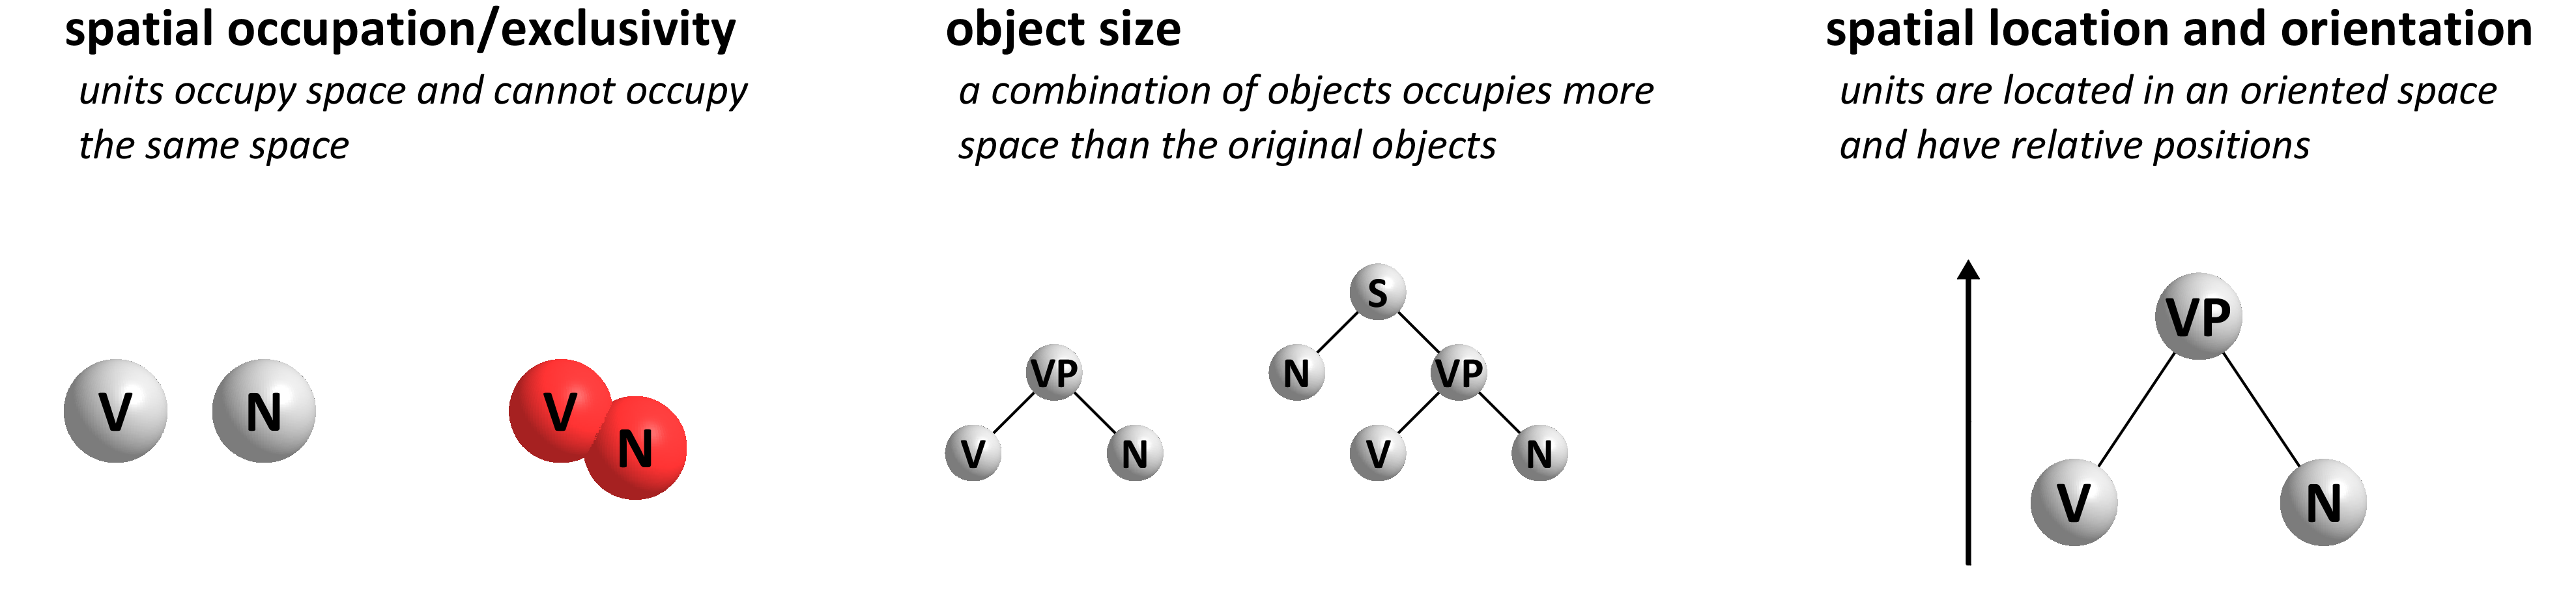
\includegraphics[width=\textwidth]{figures/Tilsen-img30.png}
\caption{\missingcaption}
\label{fig:}
\end{figure}
 

\textit{Spatial occupation and exclusivity:} objects occupy space, and spatial occupation is exclusive. My coffee cup takes up some space, and so does my granola bag. Moreover, the coffee cup and granola bag cannot occupy the same space—spatial occupation by objects is mutually exclusive. Likewise, two syntactic objects cannot occupy the same position in a structure. 

\textit{Object size:} when two objects are combined, the combined object occupies more space than either of the original objects. Objects with more parts are larger than objects with fewer parts. Likewise, combining syntactic objects creates a structure that is larger than the original objects.

\textit{Spatial location and orientation}: objects occupy a definite, unique position in an oriented space and have relative locations. The coffee cup and has a definite, unique position in space, and that position can be described relative to the definite, unique position of my granola bag. Likewise, syntactic objects are in definite positions in a structure, and phrases are above the objects which they are composed of.

  
\begin{figure}
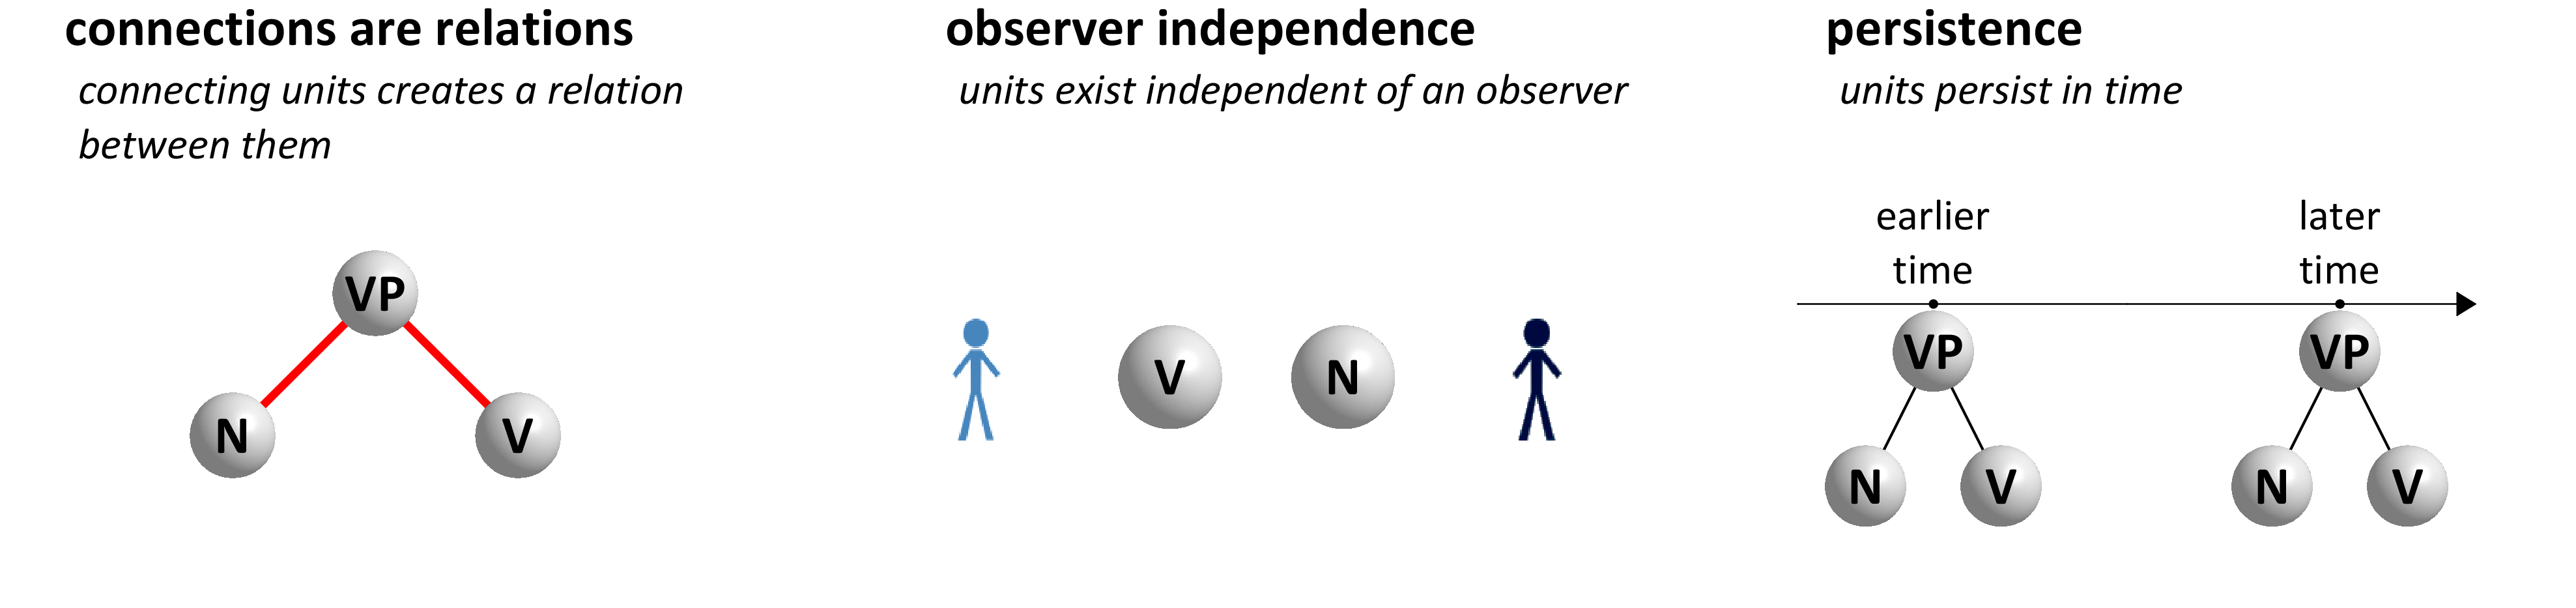
\includegraphics[width=\textwidth]{figures/Tilsen-img31.png}
\caption{\missingcaption}
\label{fig:}
\end{figure}
 

\textit{Connections are relations:} connecting physical objects creates a relation between them. The pattern of connection often has some functional importance, and constitutes a relation between the connected objects. Likewise, phrases are connected to the units they are composed of.

\textit{Observer-independence:} objects exist and have properties independently of whether they are observed. In our typical experience, the properties of the coffee cup do not depend on who observes or interacts with the cup. Likewise, the properties of syntactic objects do not depend on who speaks or hears them.

\textit{Temporal persistence:} objects persist in time unless acted upon. Our experience tells us that in the absence of other causes, the coffee cup will continue to exist, i.e. the cup will persist in space and in time. Likewise, syntactic structures do not change over time or rearrange themselves in space, unless other mechanisms cause them to.

  The mappings above are just a sample of some of the most fundamental conventional mappings, and more complicated theoretical mechanisms can be understood in terms of them. For example, consider the concepts of movement and traces. In some approaches, the wh-question \textit{What does Al drink}? is formed by first building the structure \textit{Al drinks what} and then by moving \textit{what} and leaving behind a trace, i.e. \textit{What\textsubscript{i} does Al drink} t\textsubscript{i}? The movement is necessary because meaning relations are understood as connections: since \textit{what} has a meaning relation with \textit{drink}, it should be “connected” to \textit{drink}. But the temporal order of words is not consistent with this connection pattern. Meaning relations and word order can lead to conflicting inferences regarding \textit{where} a given unit should be \textit{located} in the structure. This is problematic because an object cannot be in two places at once: the spatial location mapping holds that syntactic objects occupy a unique, definite position, just like the physical objects we are familiar with. To resolve this dilemma, many theories propose to \textit{move} the object, while leaving its original “position” “occupied” by a trace object.

  Hence theoretical devices (e.g. movement and traces) are \textit{consequences} of inferences that follow from the basic metaphors/mappings. Without these mappings, conventional theories would be vastly different. Imagine what conventional theories without identity preservation and temporal persistence would be like: syntactic objects could randomly pop into and out of existence, or morph into other types of objects. Without spatial location, syntactic objects could be in different structural locations at the same time; without spatial occupation/exclusivity, objects could occupy the same position in a structure; without type preservation, we might combine objects to create a substance.

\subsection{The container schema} 

In the conventional paradigm, \textsc{linguistic units are containers}. Words “contain” meanings. Phrases “contain” words. Sentences “contain” phrases. There is meaning \textit{in} my words, there are words \textit{in} phrases, and there are phrases \textit{in} sentences. Descriptions of linguistic structure commonly evoke a container image schema. In its most basic form, the container schema involves a boundary of a region of space. This enables mappings with an inside/outside distinction (cf. \citet{LakoffNúñez2000} for a detailed description of the container schema). Because containers are also objects, containers can be contained. Hence:

“Merge yields the relation \textbf{\textit{Immediately}}{}-\textbf{\textit{Contain}} (IC)…Iterated Merge, required in any recursive system, yields \textbf{\textit{Contain}}. Arguably Merge also yields a relation between α and β (sister)… transitive closure yields C-Command.” \citep[3]{Chomsky2001b}.

  Literally, linguistic units do not physically \textit{contain} meanings or other units. The words \textit{Al}, \textit{drinks}, and \textit{coffee}, are not physically “in” or enclosed within a phrase: one cannot open up a phrase and remove one of the units. There is no physical boundary between the inside and outside of a sentence. Yet we use container-based spatial reasoning pervasively. Below are some mappings which involve the container schema:

  
\begin{figure}
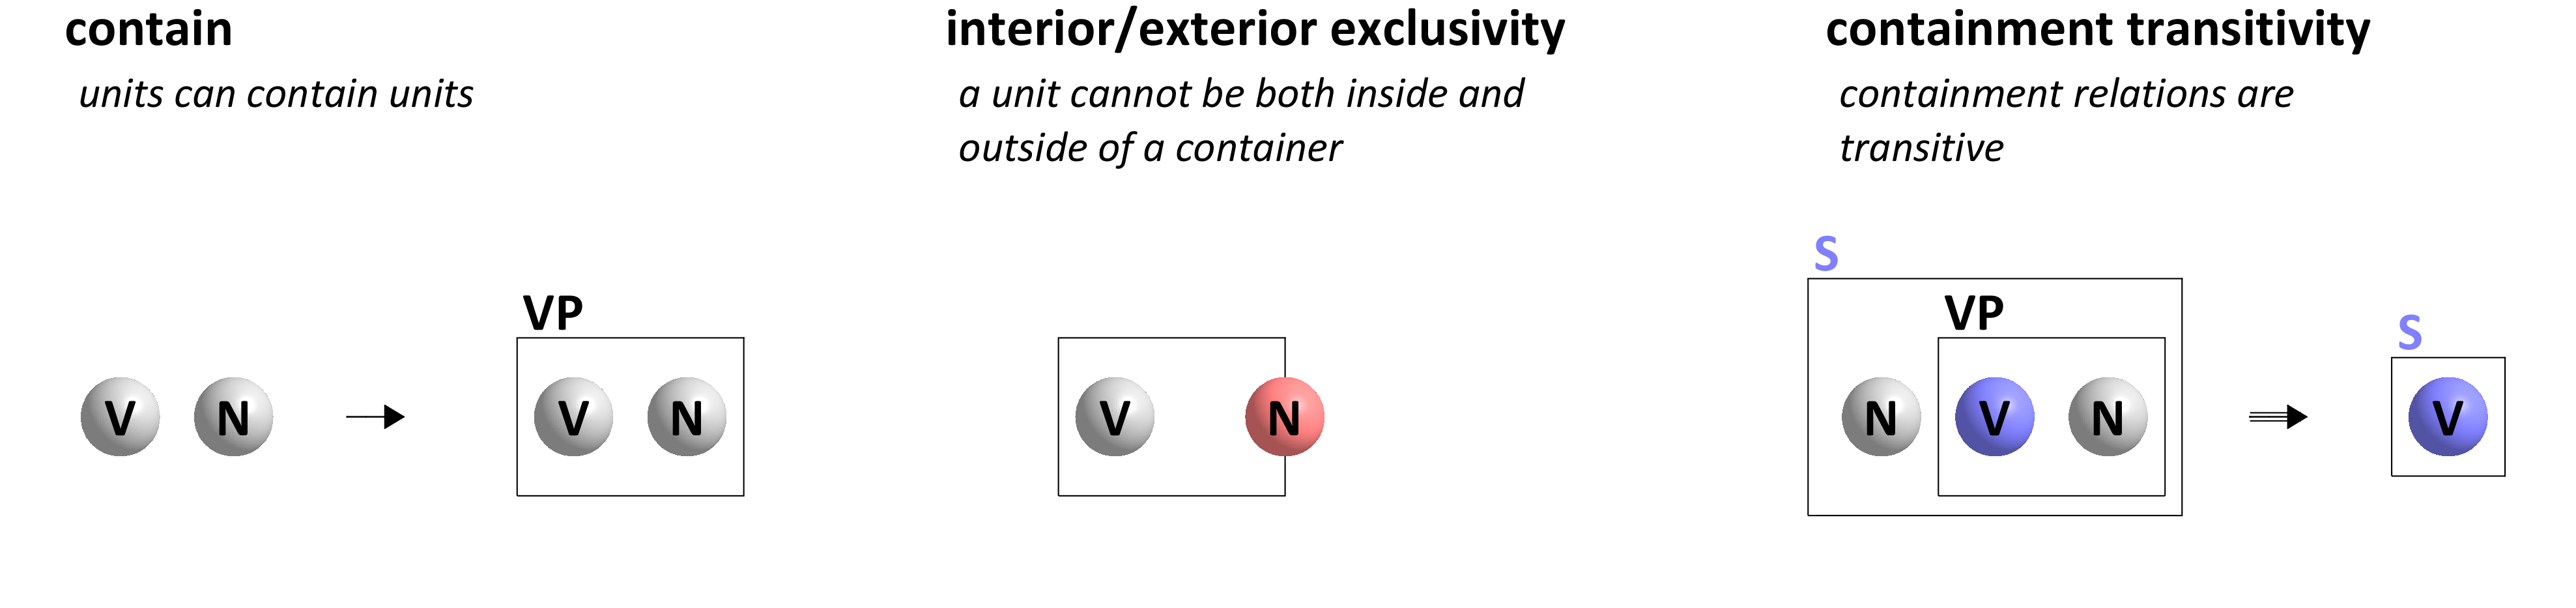
\includegraphics[width=\textwidth]{figures/Tilsen-img32.png}
\caption{\missingcaption}
\label{fig:}
\end{figure}
 

\textit{Contain:} containers can be contained. We have plenty of experience with objects being inside an object, which is inside a larger object, etc. My granola is in a bag, the bag is in my backpack, my backpack is in my office, and my office is in a building. Likewise, a linguistic unit can be inside another linguistic unit, which can be inside another linguistic unit, and so on.

\textit{Interior/exterior exclusivity}: an object cannot be both inside and outside of a container. Our typical experience is that objects are either inside or outside of a container. The granola bag is either in my backpack or not; it cannot be both inside and outside of the backpack. Likewise, a linguistic unit is either in a phrase, or not in a phrase, never both.

\textit{Containment transitivity}: if object A contains B, and B contains C, then A contains C. Given that my granola bag is in my backpack, and my backpack is in my office, we can infer via transitivity that the granola bag is in my office. Likewise, if S contains VP, and VP contains V and N, then S contains V and N.

  
\begin{figure}
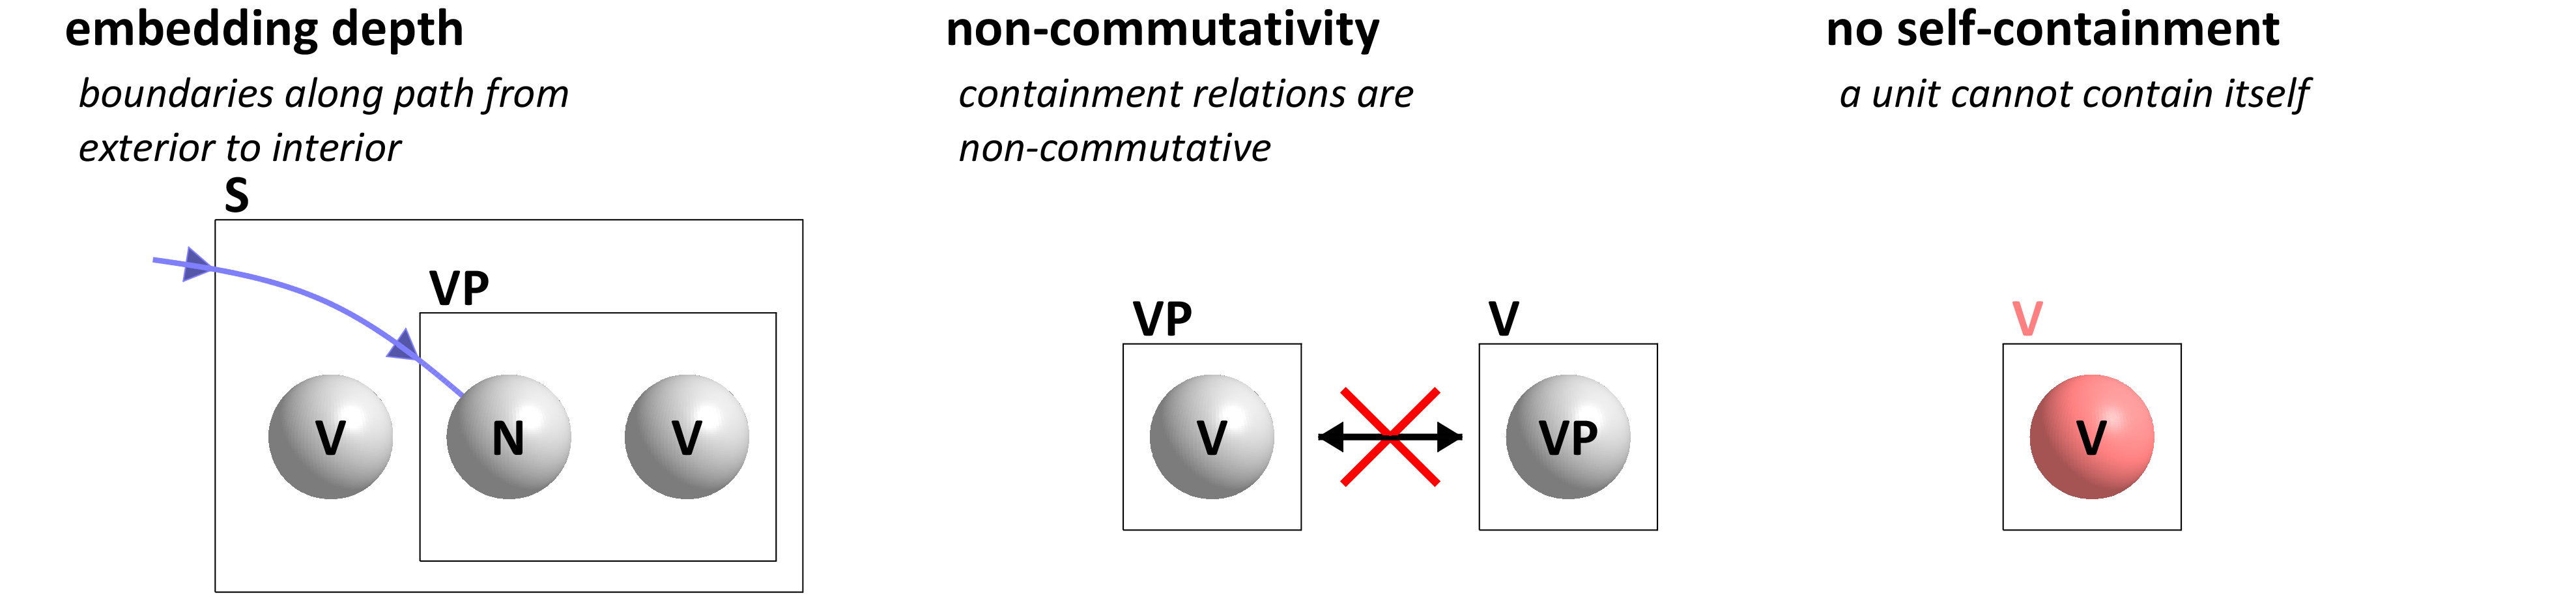
\includegraphics[width=\textwidth]{figures/Tilsen-img33.png}
\caption{\missingcaption}
\label{fig:}
\end{figure}
 

\textit{Embedding depth}: on a path from the exterior to the interior of a container, the number of boundaries the path crosses is a measure of depth of embedding. From everyday experience, we know that the length of the path can correspond to a number of boundaries encountered. Likewise, the embedding depth of a linguistic unit is measured by a count of containment relations, rather than a distance.

\textit{Non-commutativity}: an object A cannot both contain B and be contained in B. Commutative containment is so far removed from our interactions with physical objects that even imagining it is difficult. Likewise, a linguistic unit can never contain and be contained by the same unit.

\textit{No self-containment}: an object cannot contain itself, either directly or indirectly. We cannot remove an object from itself, nor put an object inside itself. Likewise, a linguistic unit can never contain itself. 

  The above mappings were probably not conscious choices in the construction of conventional theories. They are intuitive consequences of the object metaphor when objects are blended with container schemas. Some of the mappings are so essential to our reasoning that we can hardly imagine a theory without them. Why do linguistic objects never contain themselves? There is no logical necessity for rejecting self-containment, nor an empirical motivation; instead, the avoidance of self-containment of theoretical objects follows from our everyday experience with containment of physical objects. This matters because avoidance of self-containment predetermines how we construct theories. Lets consider once again the motivation for wh-movement. Why not abandon definite, unique spatial location and allow \textit{what} to occupy two positions, i.e. \textit{What}\textsubscript{i does Al drink} (\textit{what}\textsubscript{i})? The answer relates to the connection-containment blend, which we consider next.

\subsection{The connection-containment blend}

A major conceptual divide exists between constituency-based and dependency-based approaches to syntax. Constituency-based (i.e. phrase structure) approaches use a conceptual blend in which relations between units are both patterns of \textit{connection} and patterns of \textit{containment}. This blend allows for structure to be represented with trees (i.e. connected objects) and to also entail containment relations. Dependency-based approaches do not blend containment with connection schemas, and hence do not imply containment relations or phrasal structure (\citealt{Hays1964,Melʹčuk1988,Osborne2006,OsborneEtAl2011,Percival1990,Tesnière2018}). The contrast in schemas is shown below: 

  
\begin{figure}
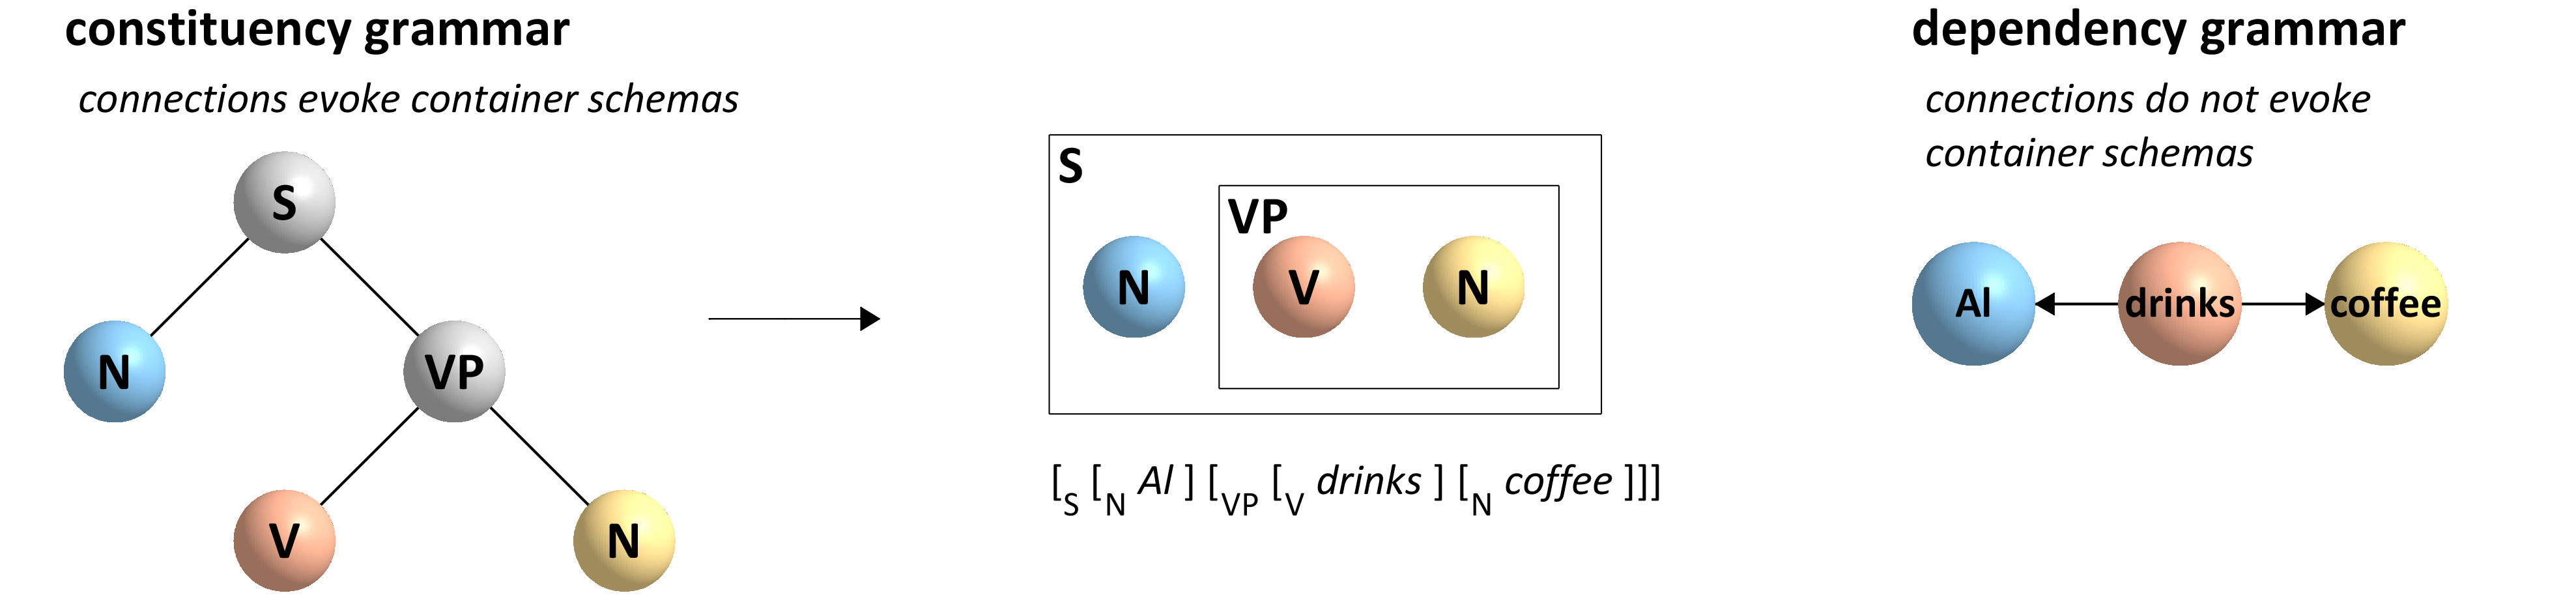
\includegraphics[width=\textwidth]{figures/Tilsen-img34.png}
\caption{\missingcaption}
\label{fig:}
\end{figure}
 

  The language used to describe aspects of connection schemas is often mapped from various auxiliary domains, such as trees, families, and networks. Hence a location in a structure where “branches” join is a “node”, an end of a “branch” is a “terminal node”. One unit can “dominate” another, or can be a “parent” or “child”, and can have “siblings”. Dominance and precedence relations can be immediate or non-immediate, depending on whether there are any nodes on the \textit{path} of connections between them. The differences between auxiliary source domains (trees, families, networks, etc.) tend to be superficial and of trivial importance. It is the more abstract and basic schema of connection, and the blending of connection with containment, which is crucial.   

  The conventional construct of a \textit{phrase} relies heavily on a blend of connection and containment schemas. Parent-child connections (i.e. dominance relations) are understood as containment relations. By convention, relational asymmetries in containment are implicit in the relative vertical locations of connected objects, with parent units located \textit{above} child units. For example in (A) below, the object N in the tree structure is \textit{inside} the VP, i.e. is a subconstituent of the VP, but the connection does not overtly show this. Containment must therefore be inferred by convention from relative orientation: N is both connected to VP \textit{and} is lower than VP. The particular direction of the orientational mapping comes from an \textit{up is more} metaphor, but one can readily imagine the reverse. The orientation of (A) is unnecessary if connections are directed, as in (B). We can thus interpret relative vertical orientation as a form of implicit directionality in connections. The orientation information greatly facilitates the containment-connection blend because it is easier to superimpose containment schemas on structures like the one in (A) than the one in (B). 

  
\begin{figure}
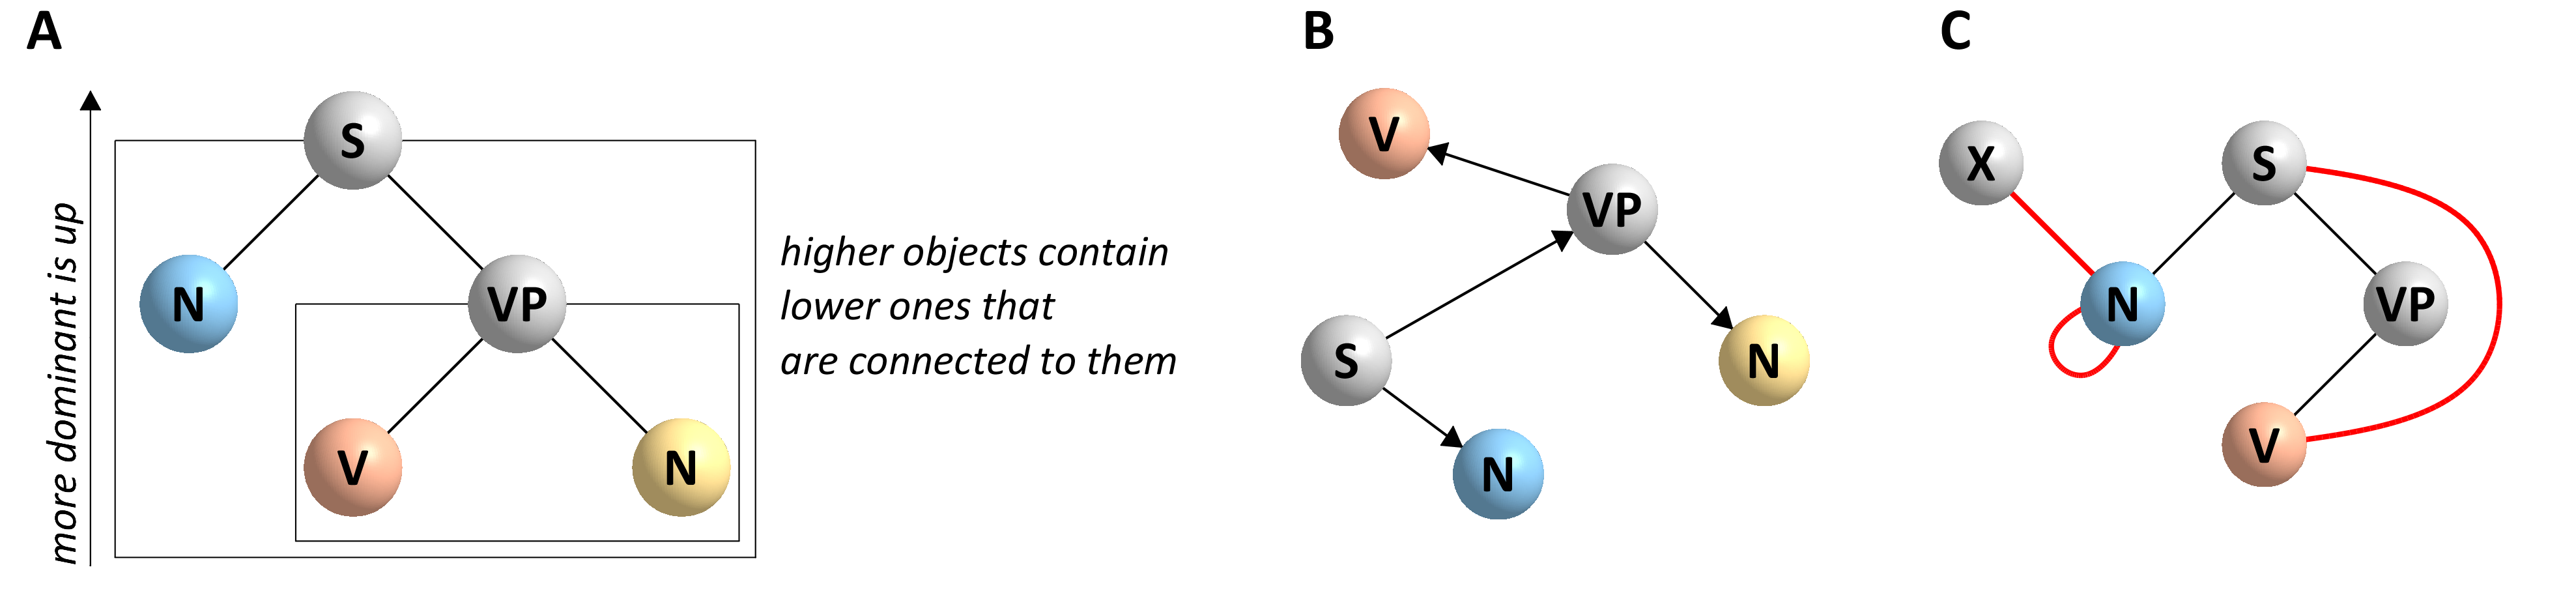
\includegraphics[width=\textwidth]{figures/Tilsen-img35.png}
\caption{\missingcaption}
\label{fig:}
\end{figure}
 

  The mappings of the connection-containment blend explain why self-connections are disallowed and why a lower unit cannot dominate a higher one. Self-connection as in (C) would imply self-containment, and allowing for lower units to dominate higher ones (i.e. abandoning the implicit orientation/directionality) would lead to indirect self-containment. A node cannot have two parents, i.e. never connects to two nodes above it, because this would lead to ambiguity in which parent container is the most external. If A contains C and B contains C, then to avoid such ambiguity either A contains B or B contains A; but the situation in example (C) where both X and S are connected to N gives rise to an ambiguity in the containment relation between X and S. Crucially, prohibitions on self-connection and multiple parents are not a necessary consequence of using connection schemas; the prohibitions arise from blending connection with containment.

  The connection-containment blend is powerful because it associates connection schemas with additional conceptual structure involving containment, without adding visual clutter to a representation. Note that there is a visual incompatibility between connection and containment, such that simultaneous depictions of connection and containment are problematic if one wishes to avoid connection paths or objects crossing container boundaries, as in (A). The blend is a useful tool because it hides this incompatibility: with just a little practice, we learn to infer containment patterns from connection patterns (and vice versa), without the need to envision both simultaneously. The use of orientation to indicate relational asymmetries makes the blend possible.

\subsection{{\textbf{The contingency of the object metaphor}}}

Why do the object metaphor and connection/containment schemas dominate linguistic theory? Does it have to be this way? Perhaps it is our early experience with the technology of writing. Written words on a page occupy physical space, so it is natural to extend that experience to abstract reasoning about language. Before written language, did humans think of words as objects? Probably not (\citealt{Linell19882005,Ong2013}), and so we must see our current conceptual frameworks as accidental, historical contingencies. This calls into question the value of those approaches. On the other hand, perhaps written words are spatially ordered because we have some species-specific cognitive predisposition for spatial order, a predisposition which may derive from our biological architecture. Even so, the object metaphor would still be contingent on evolutionary-scale forces. 

  We \textit{can} consider alternative metaphors. A fairly simple example is the \textit{substance metaphor}, which has mixing-related mappings instead of connection or containment. Lets think of the combination of a noun and a verb as a mixing of substances. Physical mixing often gives rise to a substance with new properties, which may not necessarily be predictable from the component substances; in a sense, the component substances lose their original identities. This seems analogous to the creation of idiomatic verb phrases from verbs and nouns: \textit{bite the dust}, \textit{break a leg}, etc. The point is that other mappings, which derive from other metaphors, could be on the table.

  The metaphors of the o/el framework are very different from the conventional ones, and this creates problems when using conventional terminology. The term “linguistic unit” so strongly evokes the object metaphor and related schemas, that its use is jarring in an o/el context. For example, in the o/el paradigm, we might adopt the metaphor \textsc{linguistic units are trajectories in a state space}. But this is absurd: how can a unit (as object) \textit{be} a trajectory? The cognitive dissonance here reveals just how deeply the tentacles of object metaphor have insinuated our cognitive models of language.

  Remember: there is no such thing as “a linguistic unit”. One must do some hard work to see that “units” are not and cannot be objects; instead, one should loosely associate the conventional construct of a unit with an experience corresponding to a trajectory in a state space. The dimensions of the space are excitation values (e) and phases (θ) of conceptual and syntactic systems. Relations between “units” are associated with particular geometries of trajectories in this state space. Avoiding the term \textit{linguistic unit} altogether is a good idea, because of its propensity to evoke the object metaphor. Thus we prefer to say that \textsc{linguistic patterns are system trajectories in a state space}\footnote{Linguistic patterns are understood metonymically here as the products (behaviors) which result from trajectories in a state space. Ultimately it is better not to reify language: language \textit{IS} nothing, i.e. not a thing: people act and we attempt to understand those actions; language is one of our analytical categories of actions.}.

  The dominance of the object metaphor is a cultural or evolutionary contingency, rather than a necessity. But the use of \textit{some} metaphors, whatever they are, is unavoidable. We need metaphors because the systems we want to understand—those involved in language and cognition—are so very complex, and metaphors are the tools we have for constructing understandings of complex phenomena. We should try to be more aware of which metaphors we choose, and we can choose to explore new metaphors.

\subsection{Object multiplicity}

The conventional mappings of the object metaphor, in particular spatial occupation and temporal persistence, necessitate co-presence and therefore \textit{object multiplicity}. Syntactic objects are \textit{present} in a space. What does it mean for objects “to be present” “in” a “space”? Via spatial occupation and persistence mappings, the object metaphor entails that all of the objects in a structure are \textit{there}, i.e. co-present in some space at some time. Hence for many utterances, a multiplicitous representation is necessary: multiple instantiations of a given type of object are simultaneously present. Consider the utterance shown below, \textit{Dee knows that Cam knows that Bo knows that Al drinks coffee}. The multiplicitous representation in (A) shows many instantiations of each syntactic category, and many copies of the verb \textit{knows}.

  A non-multiplicitous connected object representation as in (B) necessarily violates some mappings of the connection-containment blend. It looks very much like a finite state model (without transition probabilities), which is the very conception that generative grammar originated in reaction to \citep{Chomsky1956}. The structure in (B) violates a number of conventional mappings: containment is not transitive; there is self-containment; relative vertical orientation does not map to containment/dominance; the typical notion of embedding depth is not available. Moreover, a structure of this sort cannot be constructed through \textsc{Merge}: each word must be associated with its own syntactic object; words cannot share the same object. Hence we conclude that multiplicity is a consequence of object co-presence and connection/containment mappings.

  
\begin{figure}
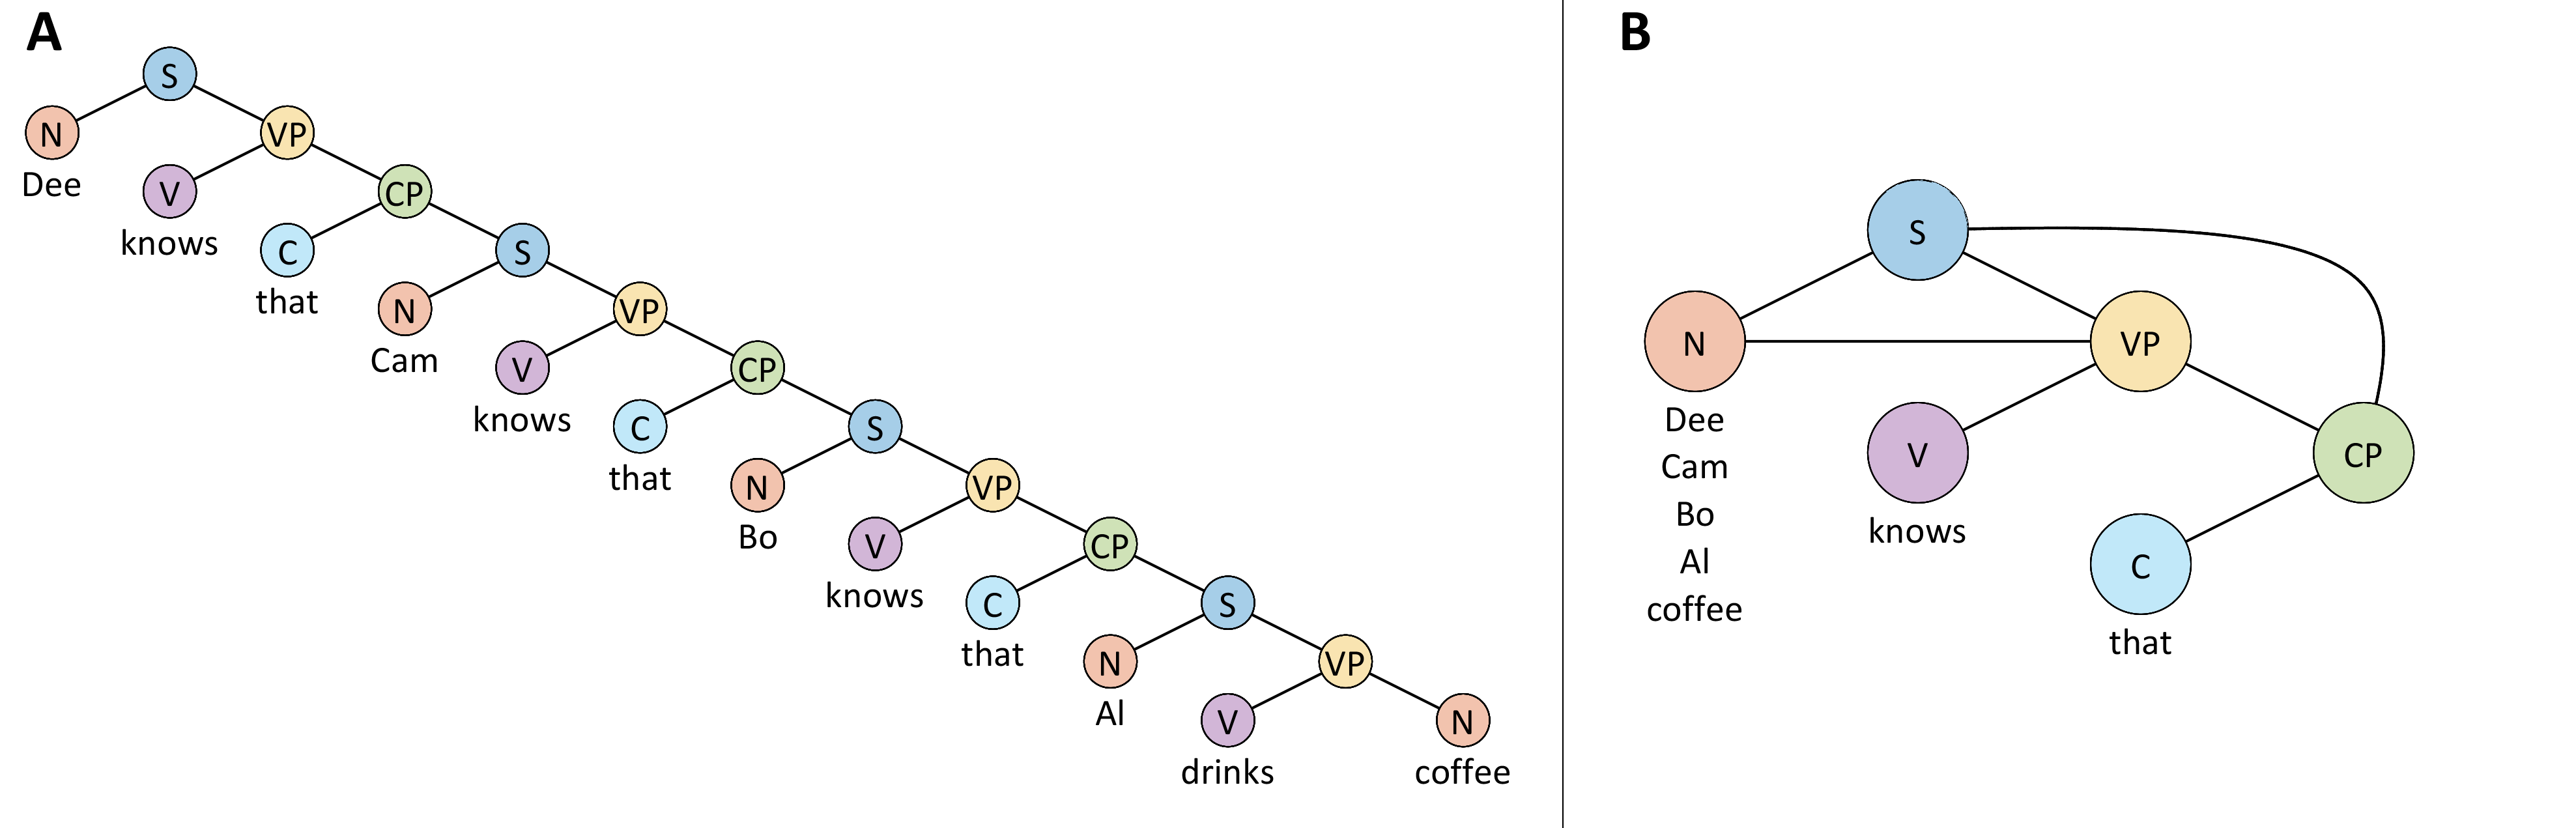
\includegraphics[width=\textwidth]{figures/Tilsen-img36.png}
\caption{\missingcaption}
\label{fig:}
\end{figure}
 

  The problem with multiplicitous representations is that they prevent us from recognizing an important phenomenon: \textit{interference}. In the o/el framework, each concept system resonates with a syntactic system. Both types of systems are, microscopically, neural populations of finite size. In order for two c-systems such as [Al] and [Bo] to simultaneously resonate with the same \{+N\} s-system, the s-system population must \textit{differentiate} into two subpopulations, where each subpopulation interacts more strongly with one or the other of the two concept populations. But this differentiation cannot be perfect: the s-system subpopulations overlap and will interact with one another, and hence the c-systems will interfere with one another, indirectly, via their resonances with the differentiated s-systems. 

  
\begin{figure}
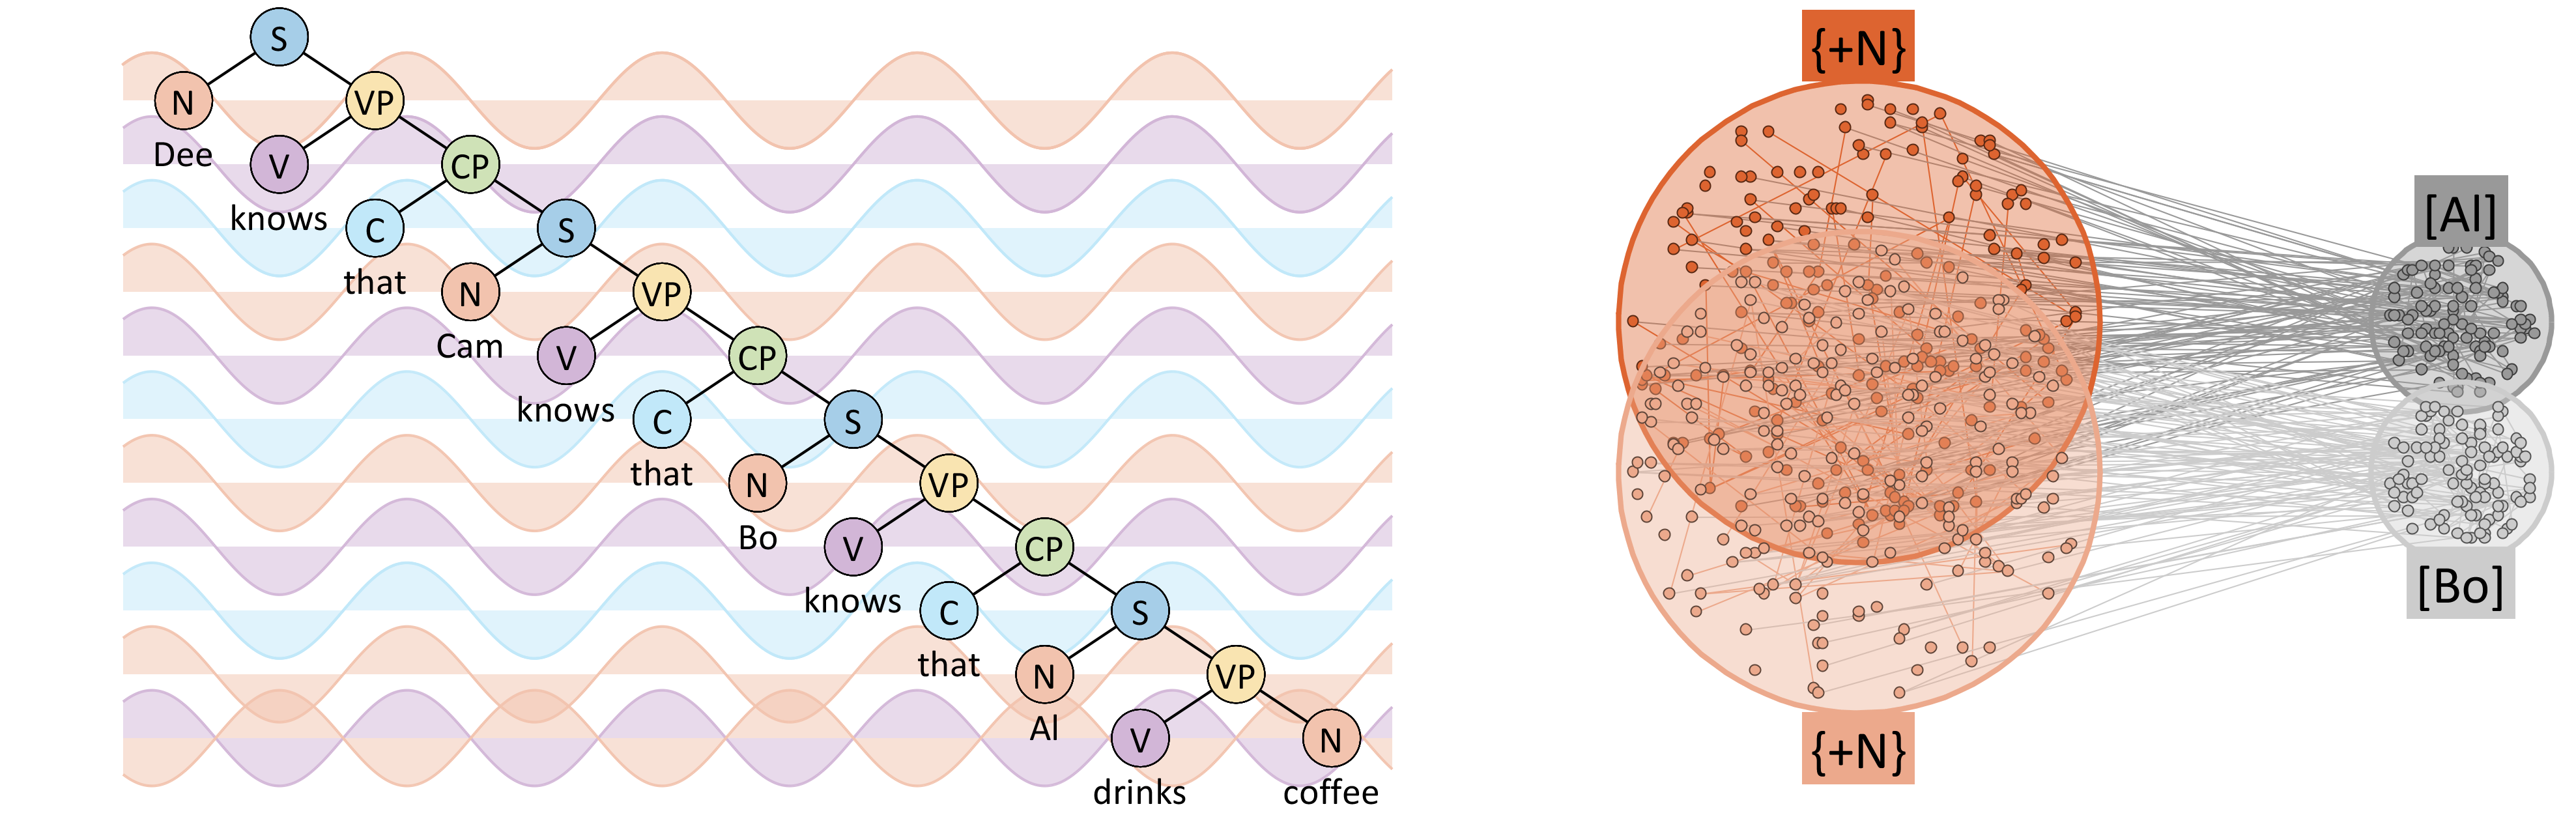
\includegraphics[width=\textwidth]{figures/Tilsen-img37.png}
\caption{\missingcaption}
\label{fig:}
\end{figure}
 

  The conventional metaphors give us no reason to expect limitations on the number of “copies” of an object. The object metaphor and connection-containment blend necessitate multiplicity. But the brain, a physical system, cannot work this way. There must be limits on the differentiation of populations, because of their finite sizes. More to the point, the brain cannot create arbitrarily many copies, or even two copies, of the same object, because linguistic units are not \textit{objects} in the first place and thus cannot be copied. In the o/el framework, we see why multiplicity is a problem, and we can explore how interference constrains the organization of syntactic and conceptual systems.

\section{The time-is-space metaphor}

In all human cultures, there are spatial metaphors/image schemas for conceptualizing time. A very general one is the metaphor that \textit{temporal order is spatial order}, or more tersely, \textit{time is space} (\citealt{Boroditsky20002001,CasasantoBoroditsky2008,Evans2006,GentnerEtAl2002,LakoffJohnson1999,NúñezEtAl2006}). In the most common variant of the metaphor, time is a \textit{linear} space. Another variant involves a periodic space, where times are locations on a circle, or phase angles. In both of these schemas, there are events and an observer, and there are two different ways in which the observer and events can be mapped to the schema. In one, the observer is moving and events are objects located in the space through which the observer moves. In the other, the observer is stationary and events are moving objects which pass by the observer. These variations are shown below:

  
\begin{figure}
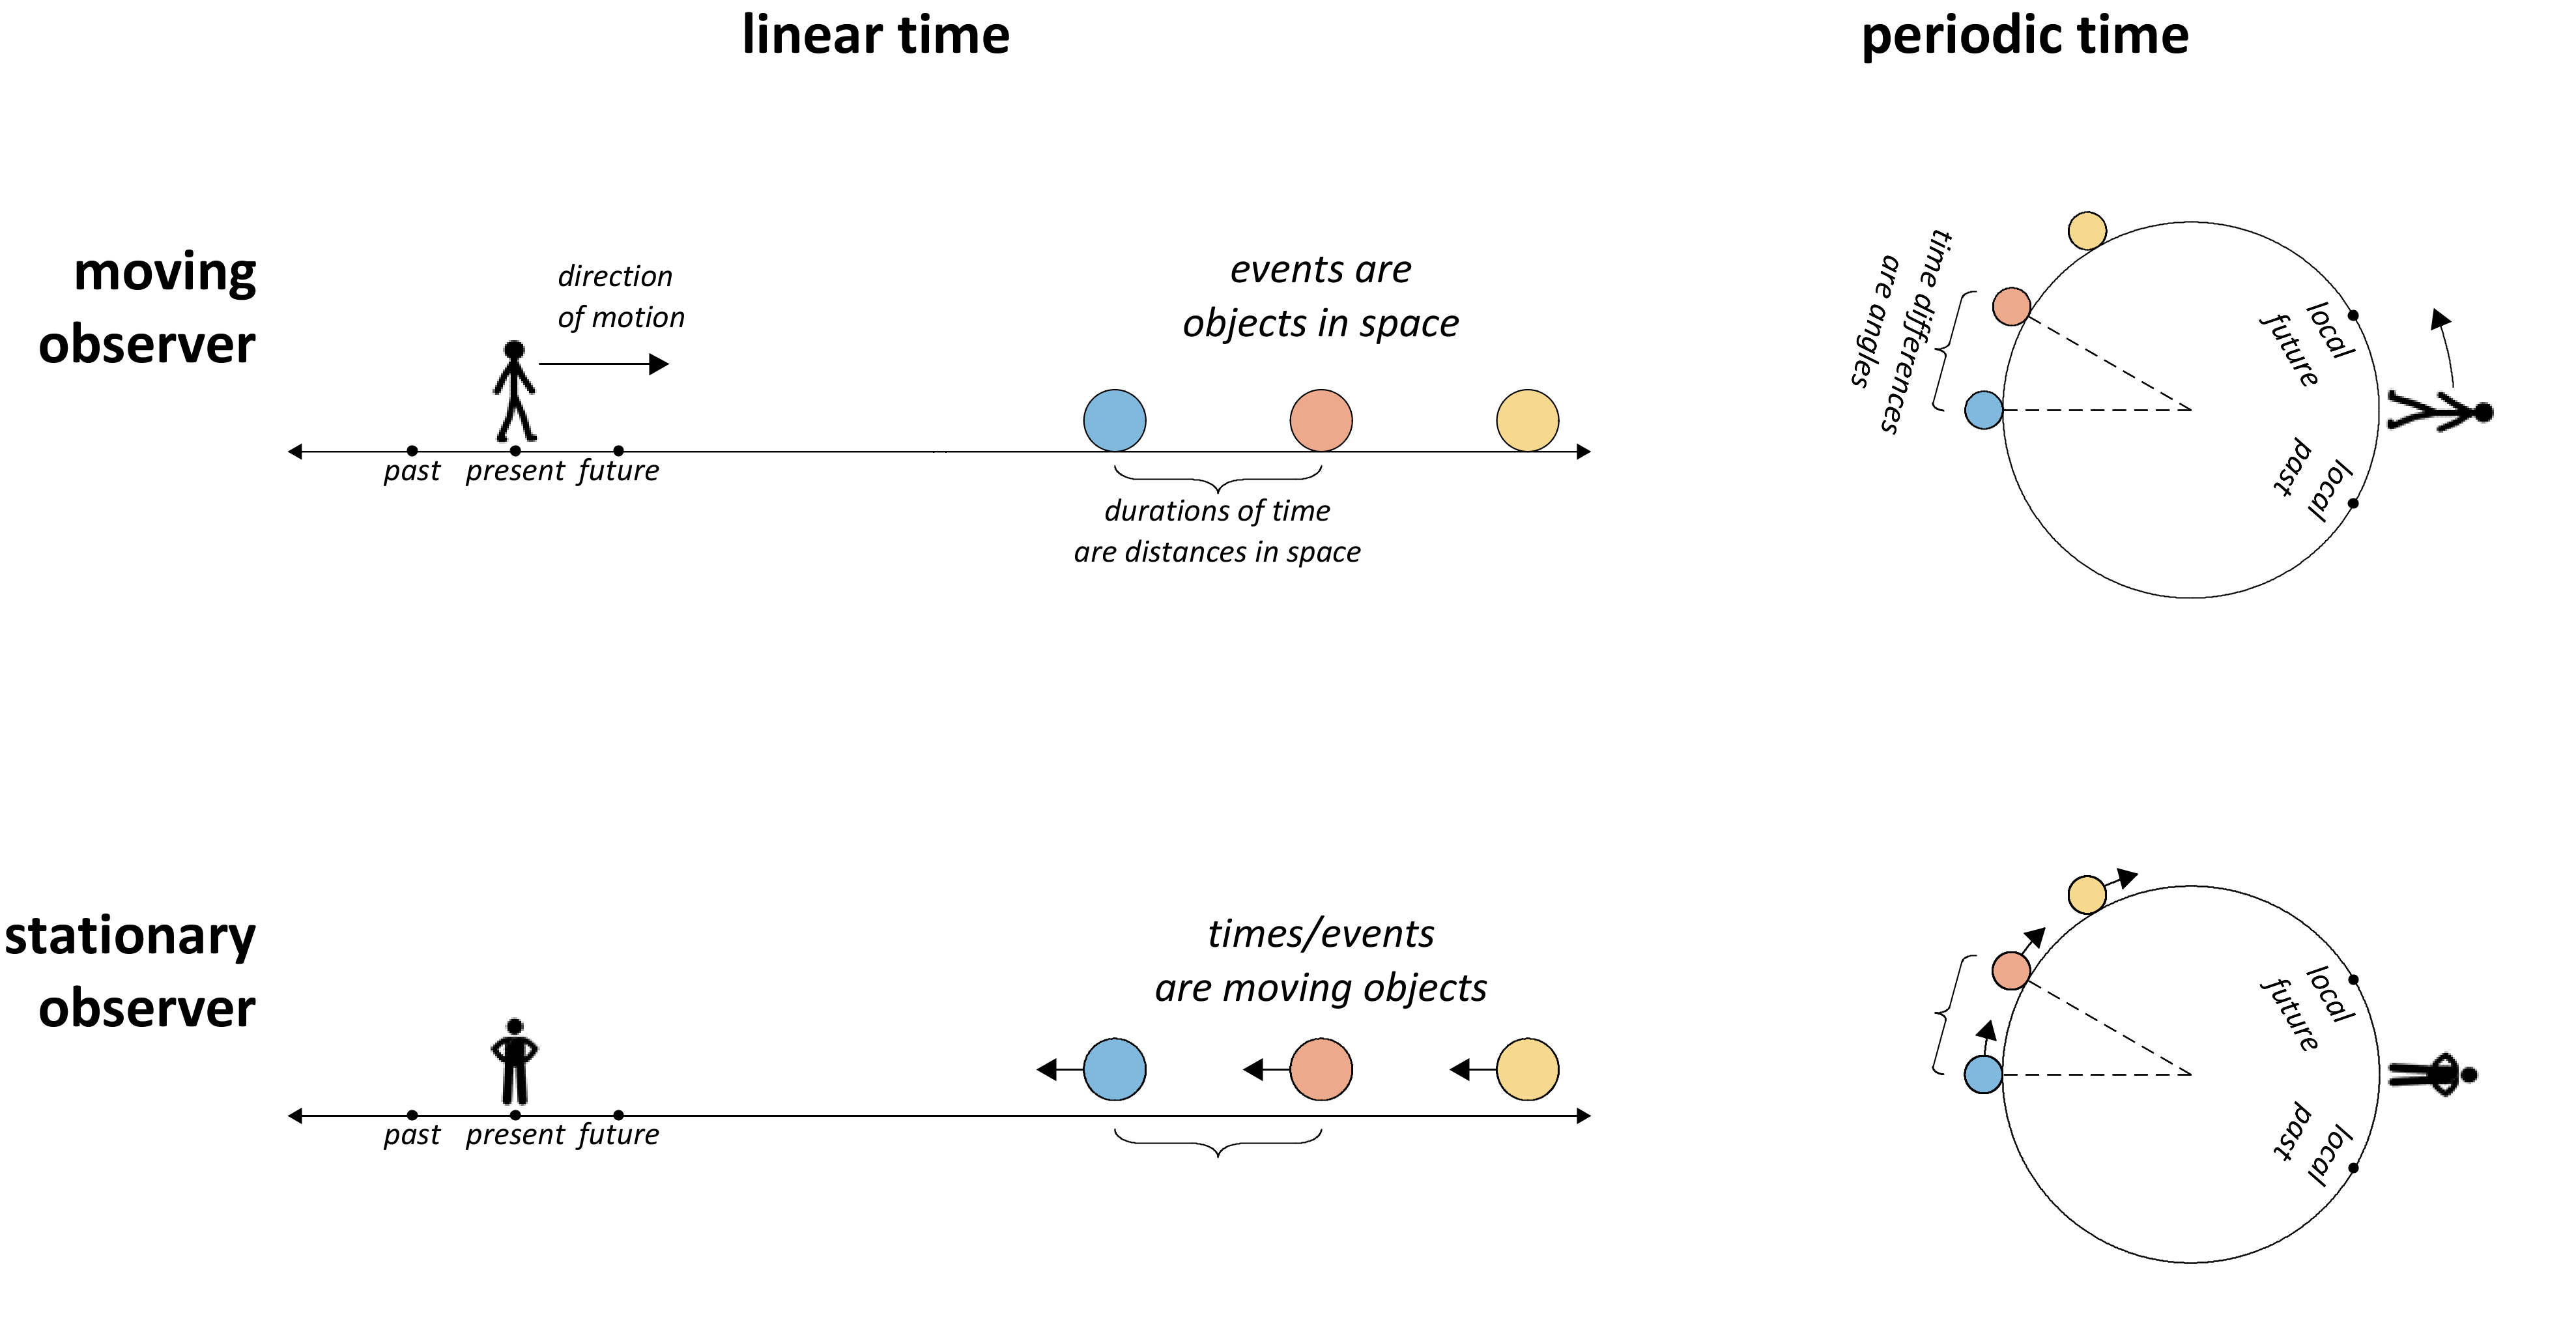
\includegraphics[width=\textwidth]{figures/Tilsen-img38.png}
\caption{\missingcaption}
\label{fig:}
\end{figure}
 

  In the moving observer linear schema, time is a landscape and an observer moves in a straight line. Events are stationary objects which are located in the landscape (or alternatively, the locations of those objects). In the stationary observer variant, the observer stays put and events are objects which move toward the observer. The moving vs. stationary observer schemas are related by a figure-ground reversal, and we quite often transition between these two schemas in everyday language. Both variants impose temporal asymmetry based on the direction of attention of the observer: the future is \textit{in front of} the observer, because direction of motion and gaze are correlated; likewise, the past is \textit{behind} the observer. These directional mappings give rise to notions of earlier and later, as well as temporal \textit{distance}. 

\subsection{The word order blend}

Words are objects; events in time are objects in space. Via the word order blend, words are objects in a space, and the space represents time. Blending a linear time schema with the object metaphor allows us to conceptualize the temporal ordering of words as a spatial arrangement. The relative order of words corresponds to their relative arrangement (position) in space: temporal order is spatial arrangement. Of course, the technology of writing reinforces this blend: written words are typically arranged in a straight line, with culture-specific variations in orientation and direction. The blend is illustrated below, for both moving- and stationary-observer variations of the schema:

  
\begin{figure}
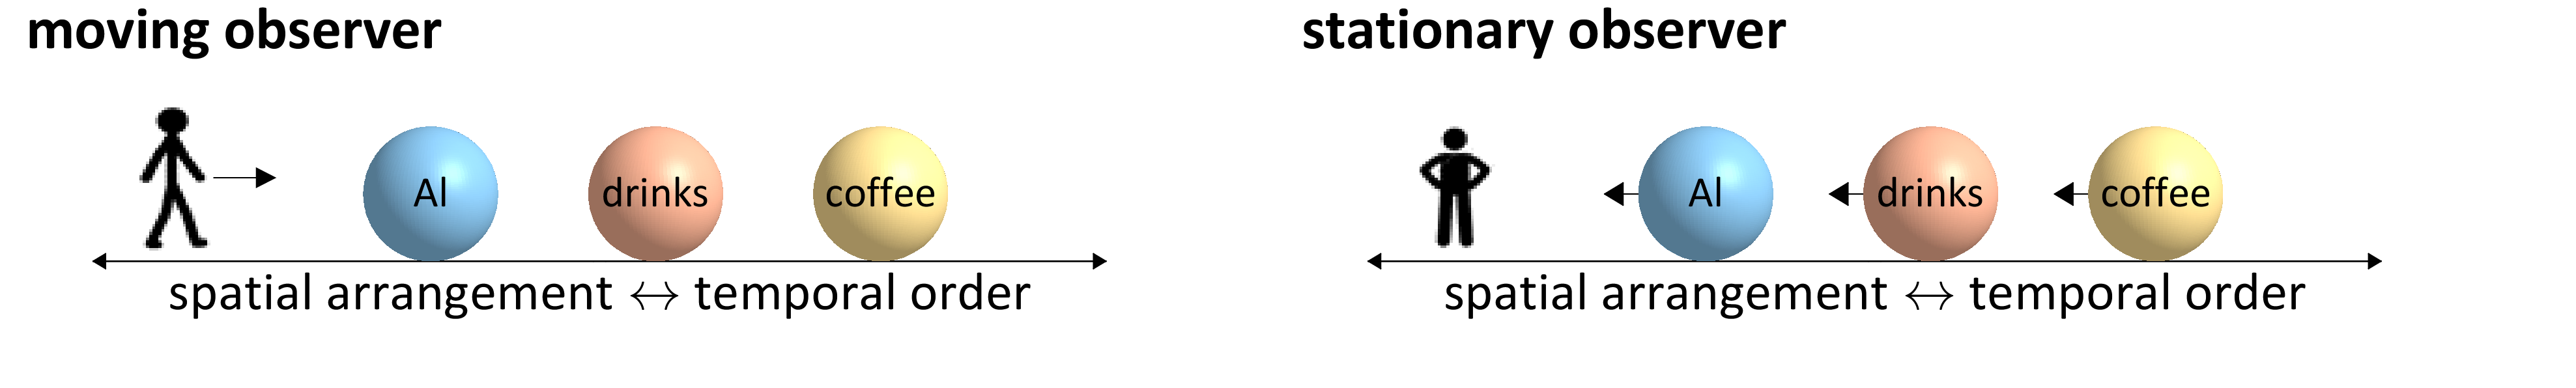
\includegraphics[width=\textwidth]{figures/Tilsen-img39.png}
\caption{\missingcaption}
\label{fig:}
\end{figure}
 

  What role does the word order blend play in conventional syntactic theories? Consider the horizontal spatial arrangement of syntactic objects in (A)-(C) below. Do all of these structures imply the same word order, or do they imply different word orders?

  
\begin{figure}
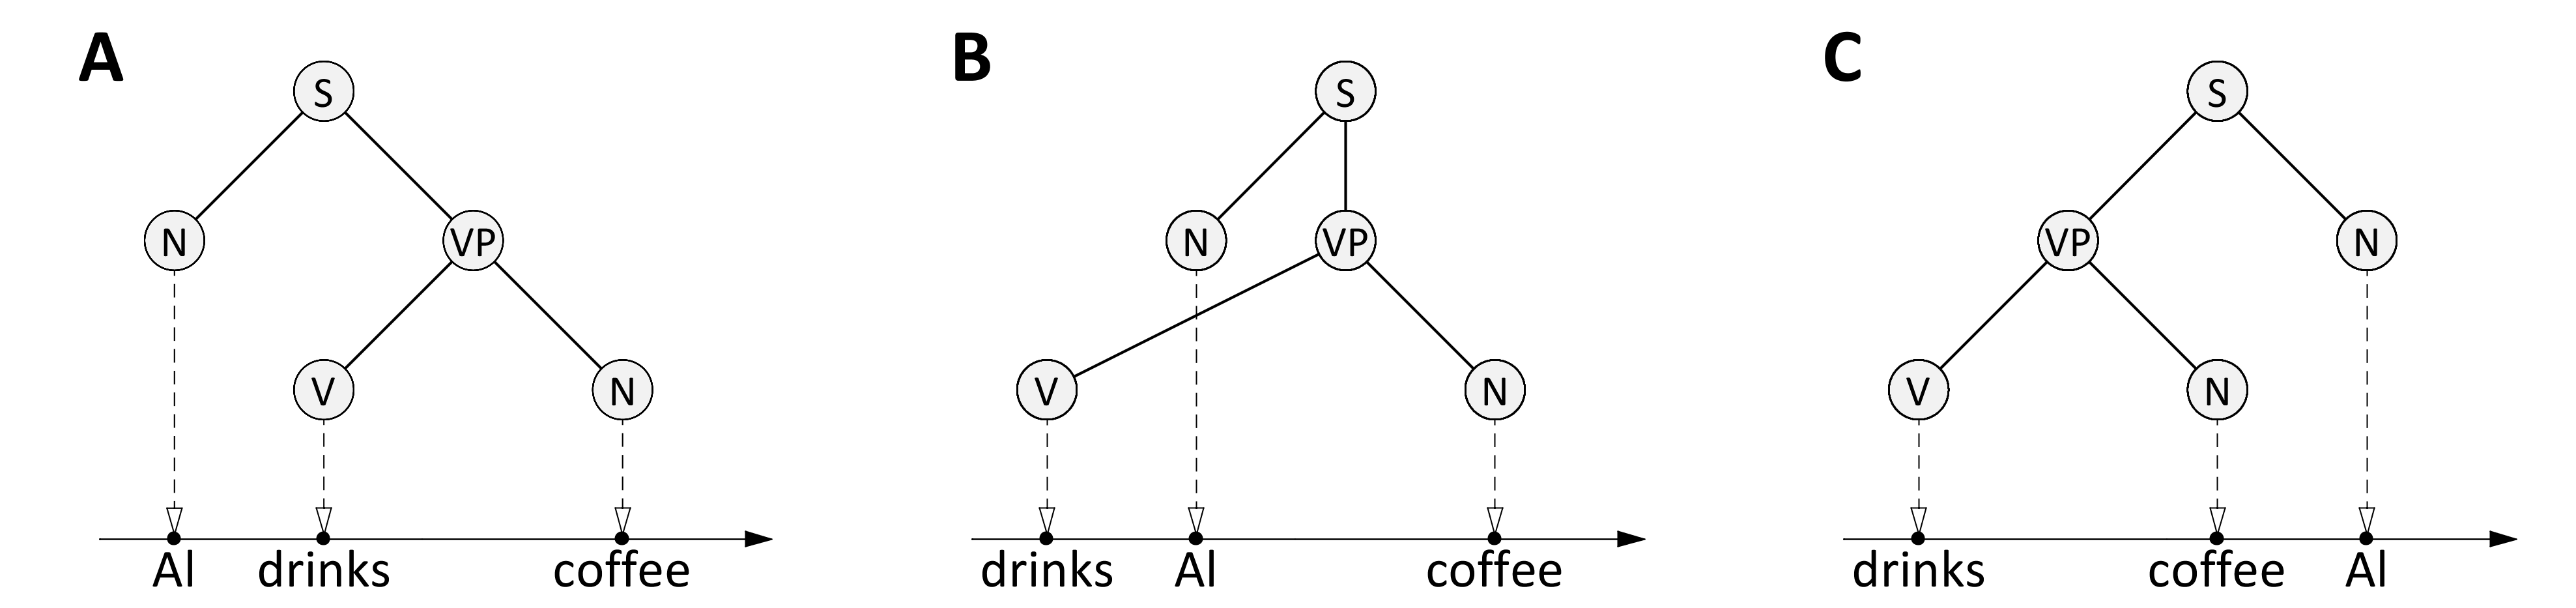
\includegraphics[width=\textwidth]{figures/Tilsen-img40.png}
\caption{\missingcaption}
\label{fig:}
\end{figure}
 

The structures (A) and (B) are not generally understood as different word orders, but (B) is a somewhat less aesthetically satisfying representation of \textit{Al drinks coffee} than (A), and structures like (B) are less commonly drawn than structures like (A). Structures (A) and (C) can imply different orders, but not necessarily. Indeed, many theoretical frameworks send mixed messages regarding the consequences of spatial arrangement in syntactic trees. Some explicitly reject the blend, but nonetheless habitually conform to it in practice. Lets consider several distinct perspectives:

\begin{enumerate}
\item \textit{The representations are explicitly temporal.}

  In this atypical perspective, representations are held to encode word order. Structures (A) and (C) must be associated with different word orders, and (B) is a bad representation of the utterance \textit{Al drinks coffee}. One can imagine projecting the terminal elements down to a horizontally oriented time axis. This axis need not represent a linear, continuous time, but simply a dimension where temporal order maps to spatial arrangement. The projection process is a simple linearization mechanism. Taking this perspective, (B) does not represent \textit{Al drinks coffee} because \textit{Al} projects down to a location between \textit{drinks} and \textit{coffee}, thereby linearizing the structure as \textit{drinks Al coffee}. (B) may also be considered a problematic representation of \textit{drinks Al coffee} because of line crossing.

\item \textit{The representations are implicitly temporal.}

  In this more common perspective, structures (A) and (C) are associated with different word orders, (B) is equivalent to (A), and (B) is a perfectly fine representation of \textit{Al drinks coffee}. Temporal order is not directly represented by horizontal spatial arrangement of terminal objects, but rather there is a universal algorithm/procedure which maps from local patterns of connection to a local word order. The antisymmetry approach developed in \citet{Kayne1994} is an example of this perspective. As shown below, we can imagine separate, local arrangement schemas are applied to each object based on its local connection structure. The local orderings are uniquely satisfied by a particular temporal order, without requiring a global mapping between horizontal arrangement and temporal order. As shown by the differences in local orderings in (i) and (ii), (A) and (C) are linearized to different word orders.

  
\begin{figure}
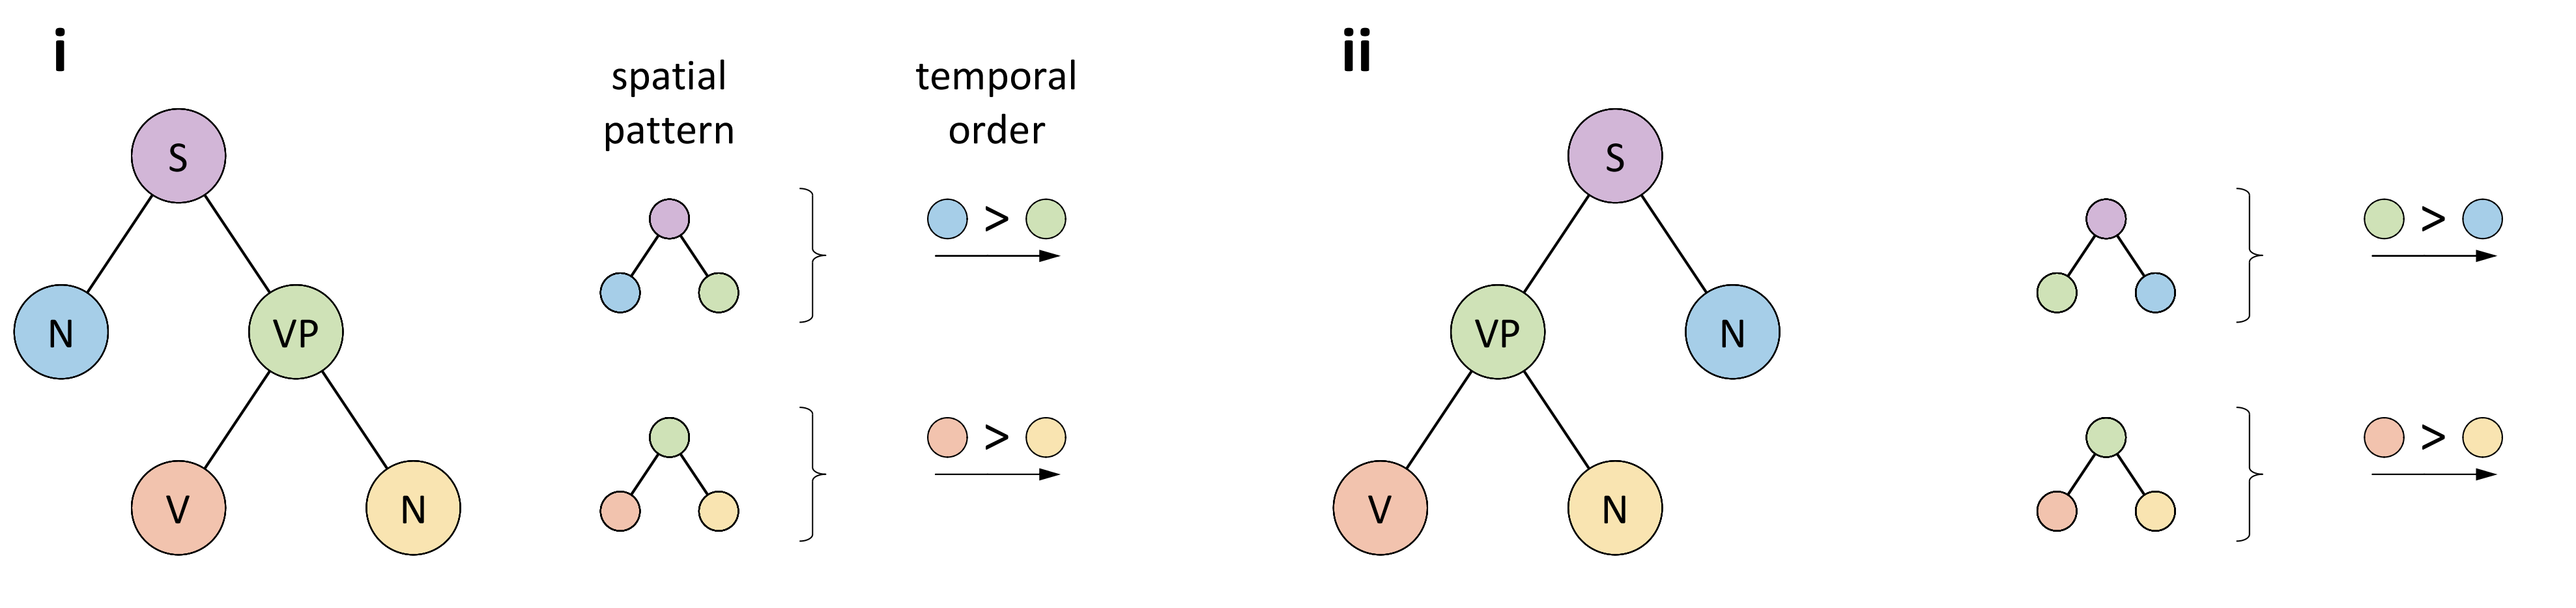
\includegraphics[width=\textwidth]{figures/Tilsen-img41.png}
\caption{\missingcaption}
\label{fig:}
\end{figure}
 

\item \textit{The representations are atemporal, linearization produces a temporal representation.}

  The most extreme perspective is that syntactic structures do not encode temporal order in any way, and so (A), (B), and (C) are equivalent. The output of merge operations, for example, is claimed to be an unordered combination of its inputs. The so-called “narrow syntax” does not represent temporal order, and all aspects of order are deferred to an independent linearization mechanism, which can vary across languages. 
\end{enumerate}


\subsection{The hidden temporality of connected object structures}

The atemporal attitude is problematic in two ways, one obvious, one deep. The obvious problem is that a syntactic theory of this sort would seem to have very little to say about word order. Many of the interesting phenomena in language involve the temporal order of words. The deeper and more important problem is that the structure building mechanism \textit{cannot} be independent of the linearization mechanism, all claims to the contrary. Any linearization mechanism must make use of \textit{some} information present in “atemporal” object structures, in order to map them to temporal orders. But if there is some temporal information in the purportedly atemporal structures, then the “atemporal” structures are not \textit{really} “atemporal”—they are covertly temporal. Moreover, this means that the output of the structure building mechanism is predetermined by the linearization mechanism. To see why this is the  case, consider the sequence of structure-building operations shown below.

  
\begin{figure}
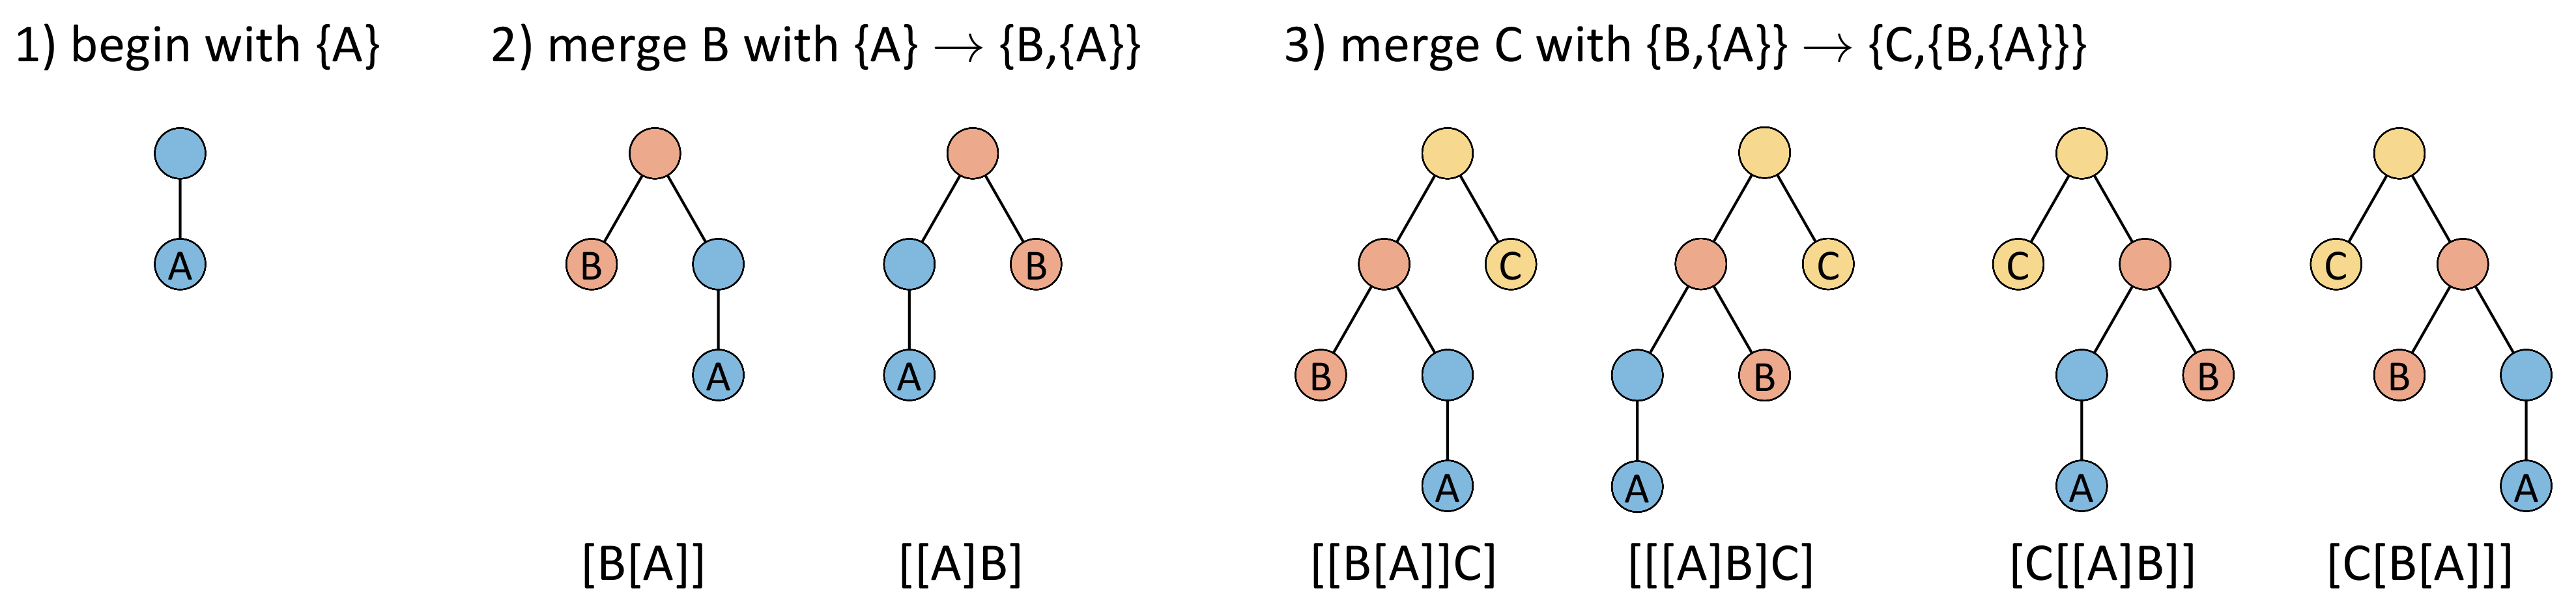
\includegraphics[width=\textwidth]{figures/Tilsen-img42.png}
\caption{\missingcaption}
\label{fig:}
\end{figure}
 

  Because \textsc{Merge} produces unordered structures, there are two equivalent representations after the first \textsc{Merge}, and four equivalent representations after the second \textsc{Merge}. These four representations can be linearized to four different orders by vertical projection, as shown below each tree structure. The same four linear orders can also be obtained from a more general linearization procedure, which we describe below.

  The CBA (right-branching) and ABC (left-branching) orders are generated by a simple iterative spell-out algorithm which proceeds up or down in vertical space. To obtain CBA, take the terminal node object from the highest level, spell it out, then move down to the next level and repeat. Observe that all four of the structures in \REF{ex:key:3} generate CBA order with this algorithm. Likewise, the procedure to obtain ABC order from all four structures starts at the lowest level and moves up. Orders BAC and CAB can be produced with somewhat more complicated algorithms which traverse the structure in two different directions. All four algorithms are shown in the {\tablebelow}. 

  \begin{table}
\begin{tabularx}{\textwidth}{XX}
\lsptoprule
CBA & ABC\\
\midrule 
\textsc{Start at highest level}

\textsc{Loop 1}

     \textsc{Find terminal node X on current level}

     \textsc{Spell X out}

     \textsc{Move down one level}

\textsc{Loop 1} & \textsc{Start at lowest level}

\textsc{Loop 1}

     \textsc{Find terminal node X on current level}

     \textsc{Spell X out}

     \textsc{Move up one level}

\textsc{Loop 1}\\
BAC & CAB\\
\textsc{Start at lowest}\textsc{/}\textsc{most embedded branching node, XP}

\textsc{Loop 1}

      \textsc{Start at highest level in XP}

      \textsc{Loop 2}

         \textsc{Find terminal node X in XP on current level}

         \textsc{Spell X out}

         \textsc{Move down one level}

      \textsc{Loop 2}

      \textsc{Move up from XP to the next branching node}

\textsc{Loop 1} & \textsc{Start at highest}\textsc{/}\textsc{least embedded branching node, XP}

\textsc{Loop 1}

      \textsc{Start at lowest level in XP}

      \textsc{Loop 2}

         \textsc{Find terminal node X in XP on current level}

         \textsc{Spell X out}

         \textsc{Move up one level}

      \textsc{Loop 2}

      \textsc{Move down from XP to next branching node}

\textsc{Loop 1}\\
\lspbottomrule
\end{tabularx}
\caption{\missingcaption}\label{tab:key:}
\end{table}

  Each algorithm generates the same order from all four of the structures in \REF{ex:key:3}. This might suggest that hierarchical structures really could be unordered, or atemporal. But there is something else to notice here. In all cases, the linearization algorithms make use of vertical orientation—information present in the structures—to determine temporal order. Moreover, the procedures require information about which nodes are branching (contain other nodes), and which are terminal (do not contain other nodes). This information is also present in the “narrow” syntactic representation. So in a sense, the information that is required for linearization, information about temporal order, \textit{is} present in the connected object representations. 

  The supposed atemporality of the representations is only a matter of perspective: either we view the structures as atemporal and view orientation and connectivity/containment information as aspects of temporalization; or, we view orientation and connectivity/containment information \textit{as temporal information that is present in the connected object structures}, with linearization making use of this information. 

  More importantly, we can see the order of \textsc{Merge} operations as a source of temporal information. Consider that, from the sequence of \textsc{Merge} operations above, two of the six possible linearizations (i.e. BCA, ACB) of \{C,\{B,\{A\}\}\} cannot be generated without some additional ad hoc mechanism. This is because B merges with A, so A and B have a more direct relation than A and C. Any linearization algorithm of the sort described above must produce an ordering in which A and B are adjacent, and therefore BCA and ACB cannot be obtained.

  The solution to this dilemma is to reorganize the structure itself with “internal \textsc{Merge}”, which is illustrated below. Internal \textsc{Merge} copies an object \REF{ex:key:2}, merges the copied object in the normal way \REF{ex:key:3}, and then ignores the original object \REF{ex:key:4}, which can involve deleting it and/or leaving a trace. The crucial insight is that internal \textsc{Merge} is necessary because the order of \textsc{Merge} operations determines the orientation and connection patterns of syntactic objects, and these in turn constrain linearization. In general, connection patterns determine which spell outs require internal \textsc{Merge}. For any structure resulting from more than one external \textsc{Merge}, there is always some set of spell outs which require internal \textsc{Merge}.

  
\begin{figure}
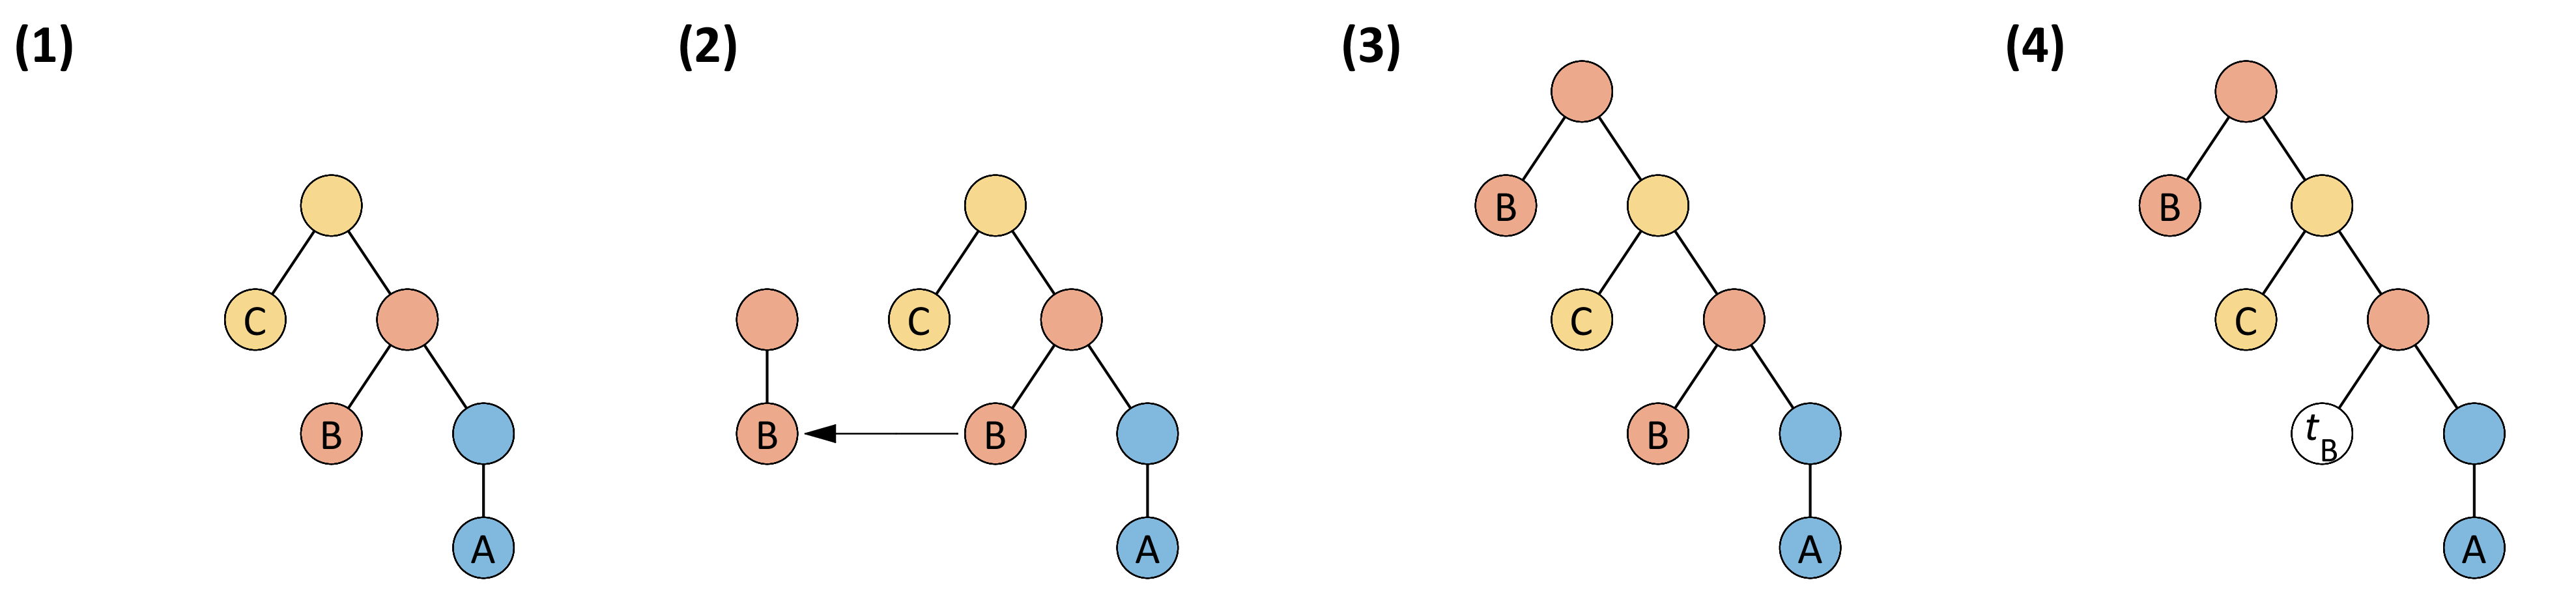
\includegraphics[width=\textwidth]{figures/Tilsen-img43.png}
\caption{\missingcaption}
\label{fig:}
\end{figure}
 

  Whether or not connected object representations are considered “temporal” is a point of view, not an essential characteristic of the representation. The linearization procedure has the property that it requires information regarding dominance (vertical orientation of connection), and so from one point of view, representation of order could be seen as an artefact of linearization, not a feature of the narrow syntax representation. But the \textit{information} needed for the linearization mechanism is present in the narrow representation itself, in the form of dominance relations and connection patterns. This is more obvious when we see that a \textit{structural} change (internal \textsc{Merge}) is necessary to generate some orders from a supposedly “unordered set”. Thus from the alternative point of view, temporal ordering information \textit{is} and \textit{always is} present in the structure. 

  Regardless of which point of view one adopts, relative vertical orientation and \textsc{Merge} necessarily interact. We can see this by comparing the outputs of top-down and bottom-up linearization schemes when applied to root-oriented and tree-oriented structures. As shown below, top-down linearization (i.e. earlier is higher) produces CBA order for a root-oriented structure, and bottom-up linearization (i.e. earlier is lower) produces ABC order for a tree-oriented structure. Thus the temporal information in orientation is implicitly determined by how \textsc{Merge} operates, or vice versa, the operation of \textsc{Merge} is determined by our construal of orientation. The fact that orientational ambiguity renders order ambiguous reinforces this point.

  
\begin{figure}
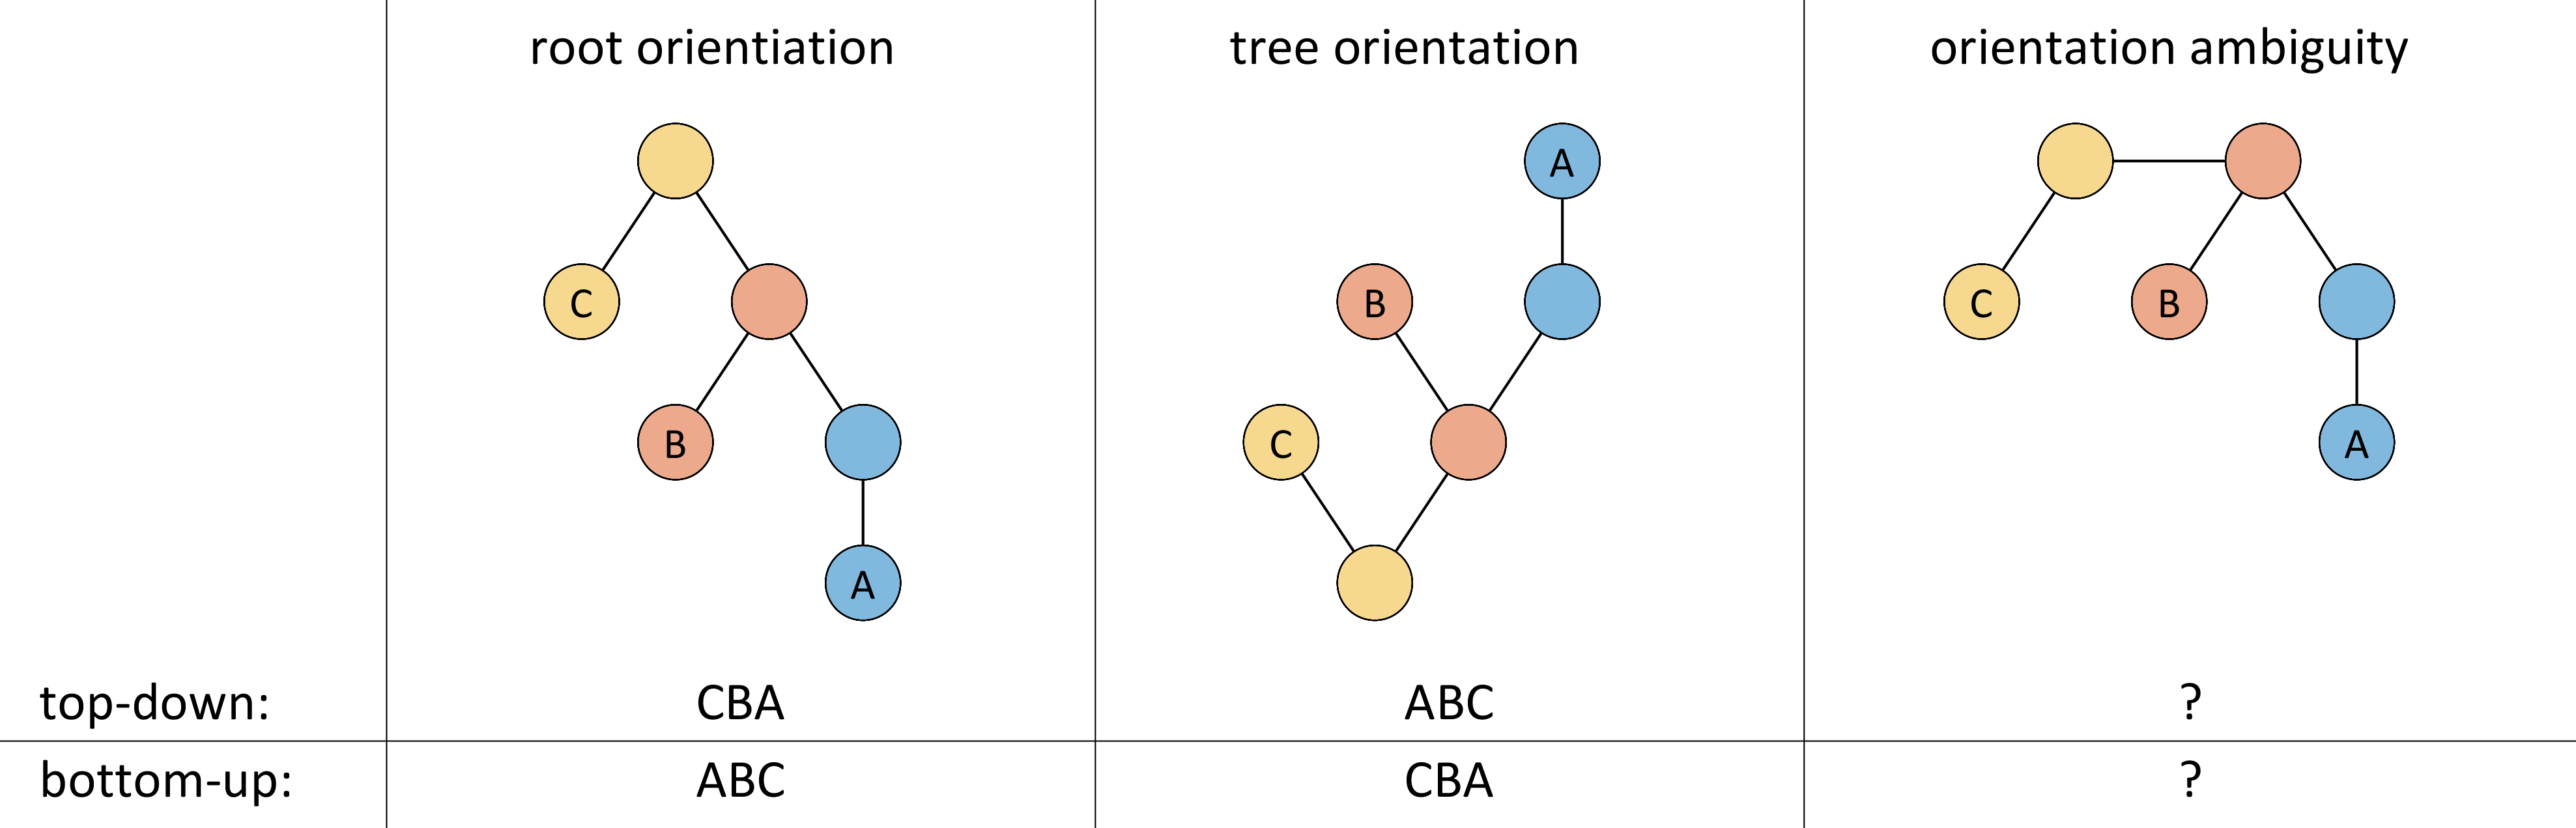
\includegraphics[width=\textwidth]{figures/Tilsen-img44.png}
\caption{\missingcaption}
\label{fig:}
\end{figure}
 

  Evoking connected object schemas is dangerous because the more we do it, the more we become habituated to conceptualizing language in this way. Nonetheless, the above discussion was necessary because it leads to the conclusion that \textsc{Merge} does not produce atemporal structures—information regarding order is always present. As others have pointed out (e.g. \citealt{Yang1999}), a truly “unordered” representation would be \{A,B,C\}, equivalent to:

  \{A,B,C\} = \{A,C,B\} = \{B,A,C\} = \{B,C,A\} = \{C,A,B\} = \{C,B,A\}

The supposedly “unordered” sets below merely obscure information regarding temporal order:

  \{\{\{A\},B\},C\} = \{C,\{A\},B\}\} = \{\{B,\{A\}\},C\} = \{C,\{B,\{A\}\}\}

Any linearization mechanism, without additional information, requires ordered structure. Concealing temporal order in vertical orientation and connection patterns, or in containment and embedding patterns, does not eliminate temporal order; it merely makes the temporal information more difficult to identify. 

\subsection{Essential vs. effective time}

The output of linearization is conventionally conceptualized with a linear time schema. This linear time schema is very general, underlying the conception of speech as a \textit{string} of words (moving observer) or as a flow/stream of words (stationary observer). What makes these conceptions of time “linear”?  The linearity is not simply the property that time is mapped to a \textit{straight line} or a \textit{straight trajectory}. The fundamental character of linearity is that any given segment of space/time is equivalent to any other one, no matter where/when those segments are located/occur, as long as those segments are the same length/duration. 

  Linearity implies a straight line relation between \textit{essential time} and \textit{effective time}. Effective time is an analytical tool, a made-up dimension of time, viewed as orthogonal to essential time. Essential time is a dimension of time that corresponds to our folk understanding \textit{what} time \textit{is}, i.e. our intuitive assumptions that time is absolute, progresses uniformly, and is independent of the observer.

  
\begin{figure}
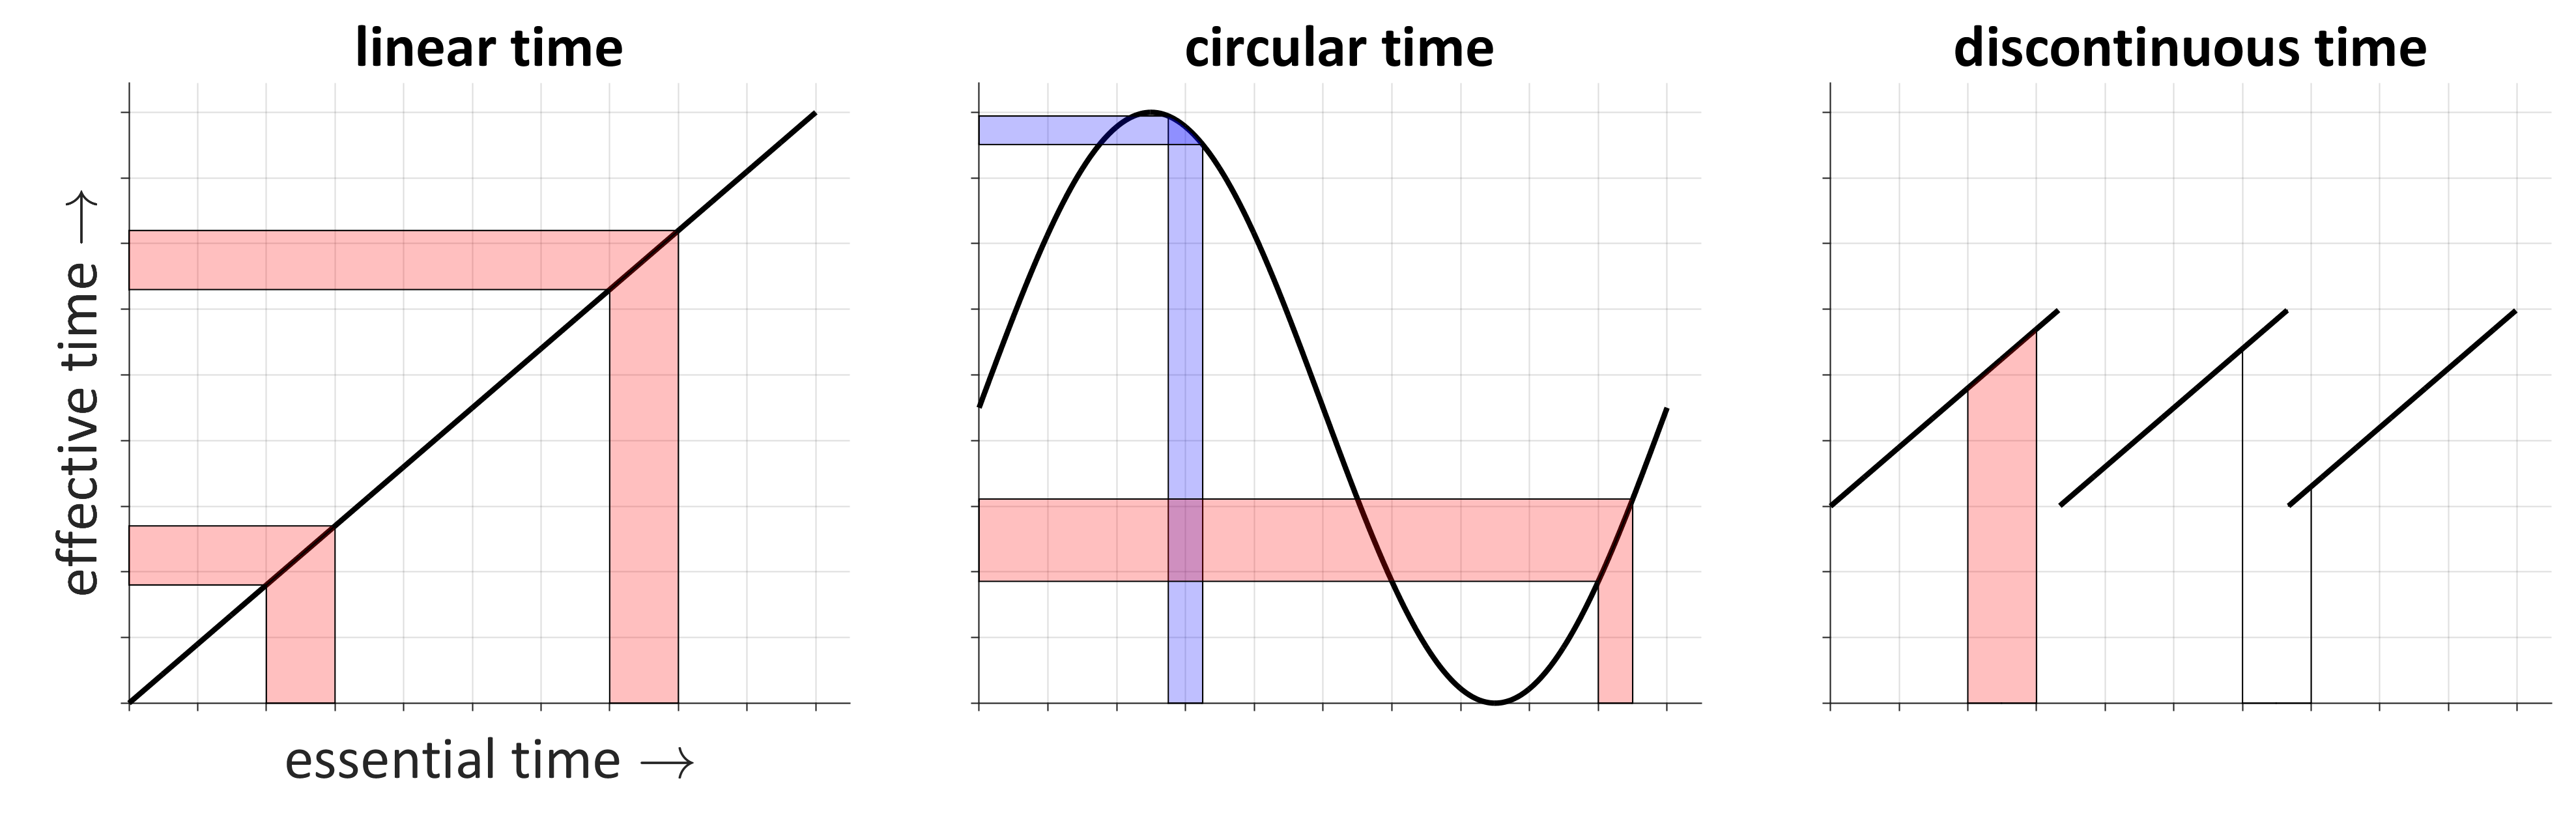
\includegraphics[width=\textwidth]{figures/Tilsen-img45.png}
\caption{\missingcaption}
\label{fig:}
\end{figure}
 

  Effective time is associated with a measure of a quantity that accumulates as essential time progresses. Consider for example an effective time quantity which accumulates at a constant, non-zero rate. For an interval of essential time of a given duration, the amount of the quantity accumulated during the given interval will be the same, regardless of \textit{when} the interval occurs. In linear time, the function relating essential time to the effective time quantity has a constant first derivative and all higher-order derivatives are zero. For example, linear time is appropriate for describing a person walking at a constant pace. If the number of steps taken is the accumulating quantity, and thus the measure of effective time, then the functional relation between essential time and effective time is a straight line. The choice of the quantity to measure is arbitrary. What is crucial is that we evoke a schema in which temporal distance maps to spatial distance, and in which this occurs in a \textit{linear} manner.

\subsection{Periodic time}

Another useful conception of time is one in which the effective time quantity is a periodic function of  essential time. This enables us to equate any moment with a set of past and future moments, leading to a picture of a closed-loop time axis, and hence phase angle, θ. Periodic time is useful in the o/el framework because variation in the order parameters of conceptual and syntactic populations is conjectured to have an oscillatory component.

  
\begin{figure}
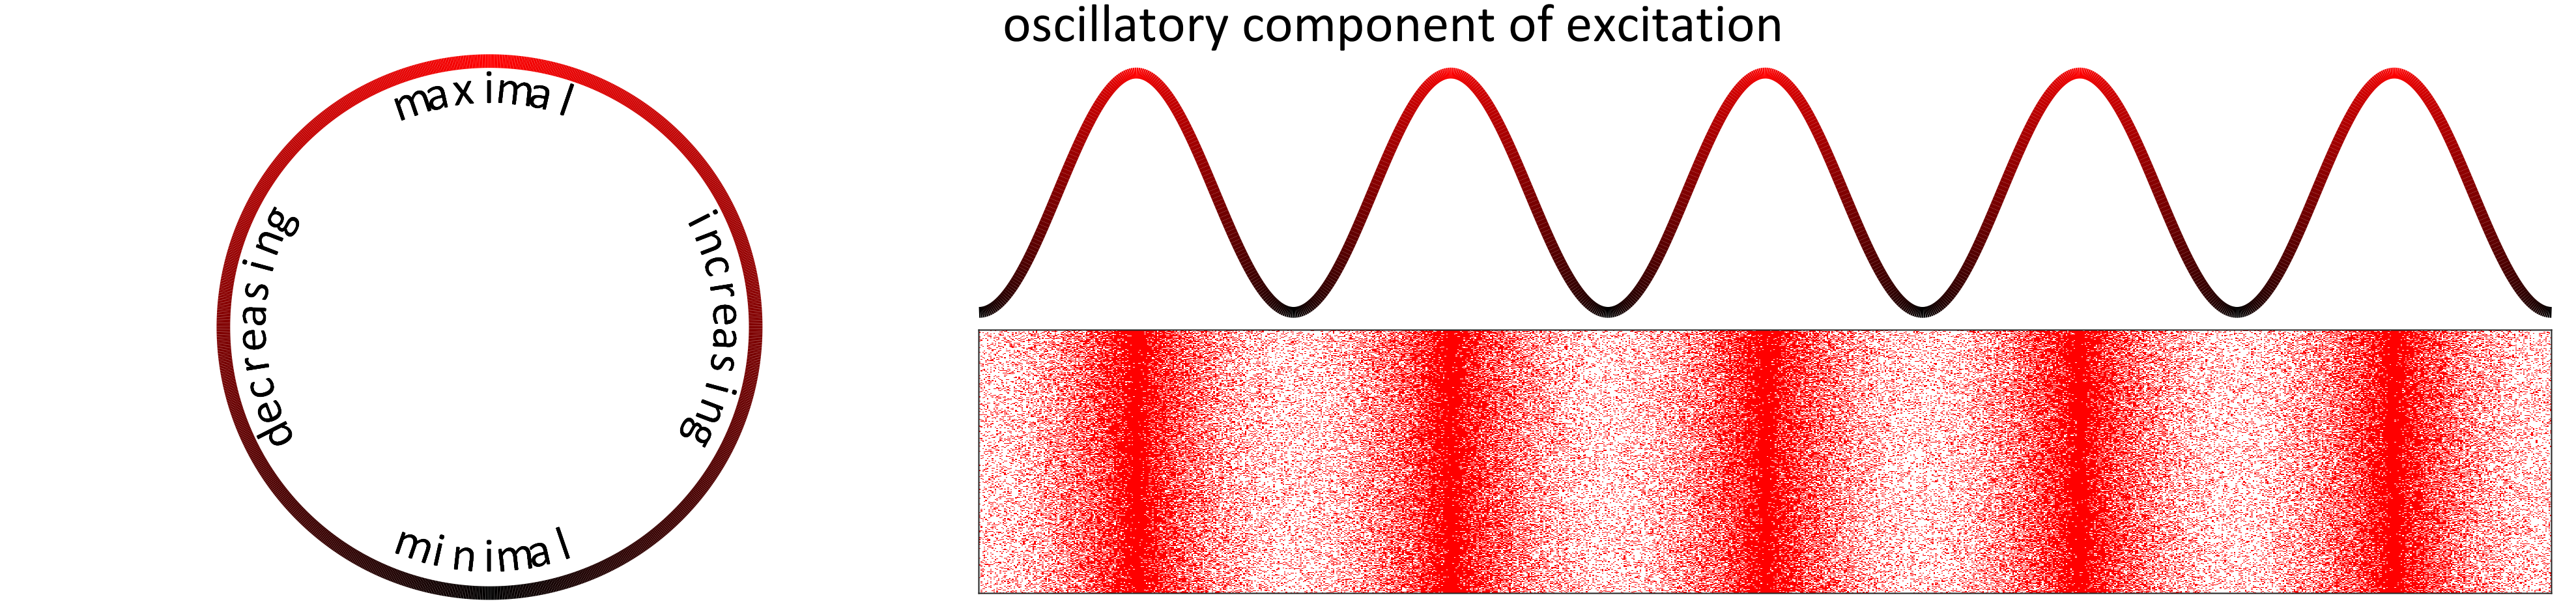
\includegraphics[width=\textwidth]{figures/Tilsen-img46.png}
\caption{\missingcaption}
\label{fig:}
\end{figure}
 

  From a macroscopic perspective, the effective time quantity of a system is θ(t). On the microscale, we can construct the oscillatory component of the order parameter to be \textit{x}\textsubscript{osc} = α sin θ and so its derivative is α cos θ. If we define the reference phase as θ = 0, then θ = 0 is when \textit{x} is maximally increasing, θ = π/2 is when \textit{x} is maximal, θ = π is when \textit{x} is maximally decreasing, and θ = 3π/2 is when \textit{x} is minimal. However, this particular mapping of θ to population microstates is an arbitrary consequence of our choice of reference phase and counterclockwise direction of motion. There is no reason, other than convenience, not to reformulate the relation with 12:00 as a reference or as a clockwise motion in Cartesian coordinates. We have also assumed for simplicity that the oscillations are approximately harmonic, but one can imagine a number of alternatives as below. What is crucial is not the precise form of the oscillation, but rather its periodic nature, which entails symmetry under rotations of 2π radians. Accordingly, there is a discrete time-translation symmetry in essential time, under integer multiples of translations of T = \textit{f}\textsuperscript{{}-1} = 2$\pi \omega $\textsuperscript{{}-1}, where \textit{f} is the frequency in cycles/sec, ω is angular frequency in radians/sec, and T is the cycle period.

  
\begin{figure}
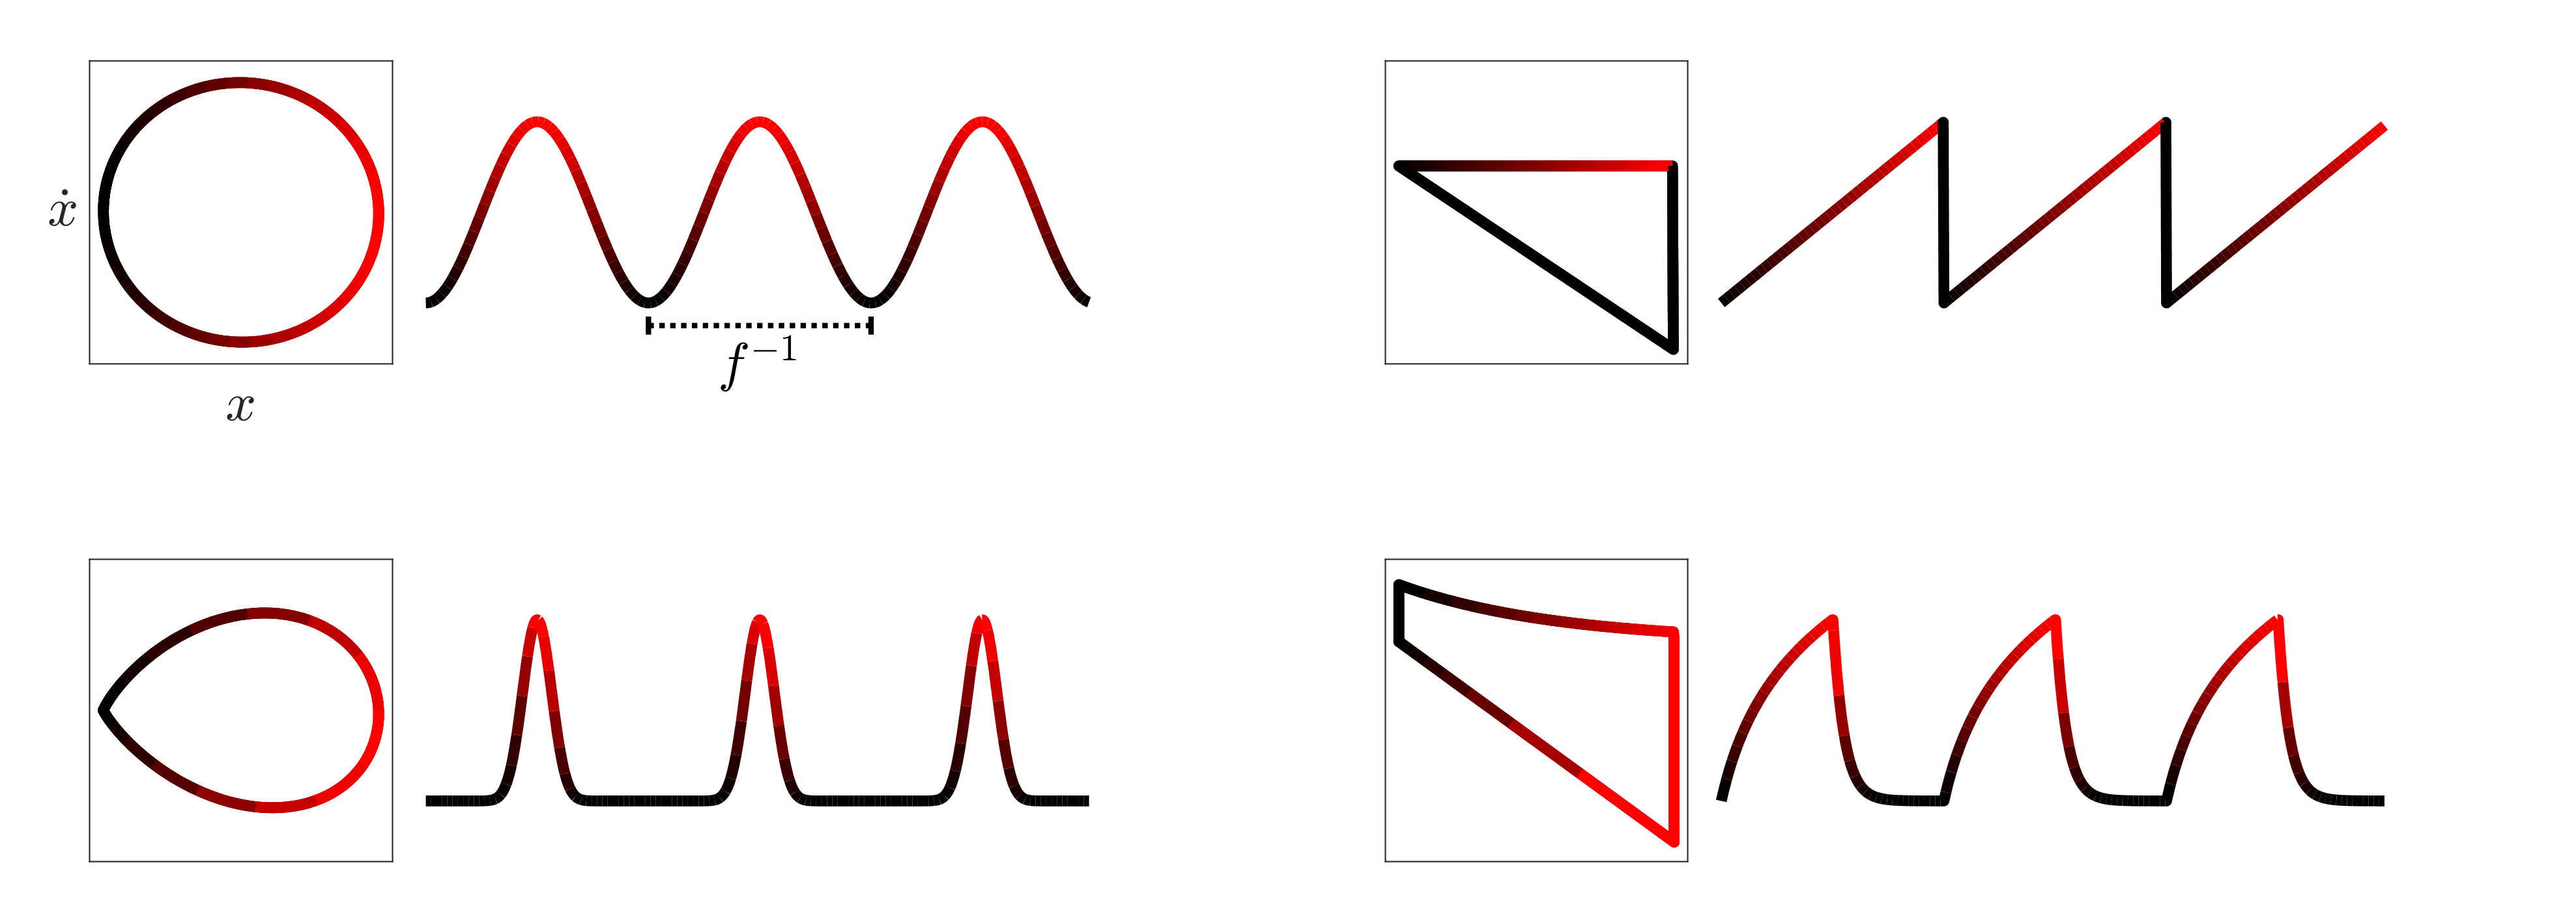
\includegraphics[width=\textwidth]{figures/Tilsen-img47.png}
\caption{\missingcaption}
\label{fig:}
\end{figure}
 

  Because of its discrete time translation symmetry, periodic time has only local notions of past, present, and future. There is no global past/future in a periodic time schema because the time axis, though unbounded, is finite. A moving observer, who is at some location (θ), will eventually return to that same location. There is also no inherent way to decide which location is visited first: the moving observer can only decide that some particular phases are visited \textit{relatively} before or after others, where the qualifier \textit{relatively} expresses the locality of the relation, which must be less than (2\textit{f})\textsuperscript{{}-1}, i.e. less than half the period of the cycle. Likewise, a stationary observer will experience the same sequence of events forever, but has no inherent way to decide which event begins the sequence. Hence circular time has no global conception of temporal order, only a local one. 

  Why is the absence of a global past and present important? The principle of relational meaning holds that relational meaning experiences are stable φ patterns. Periodic time provides a more natural description of this condition, since φ is invariant despite change in θ. Moreover, in a periodic time schema, the minimal and maximal φ differences between systems are 0 and ±π, and these are the two φ configurations we are most interested in. Thinking of such relations in terms of linear time obscures this form of temporal invariance. For example, variation in arousal and other surroundings mechanisms may induce variation in the absolute timing of spike rate maxima of populations, i.e. variation in Δt. Such variation is illustrated in the {\figurebelow}, which shows waveforms of different frequencies. However, by factoring out such variation with the relation 2π\textit{f}Δt = $\omega \Delta $t = φ, we can ignore irrelevant differences in absolute timing and recognize a fundamental invariance in relative phase. The frequency \textit{f} can thus be viewed as a normalization device, a tool for factoring out variation we are not interested in.

  
\begin{figure}
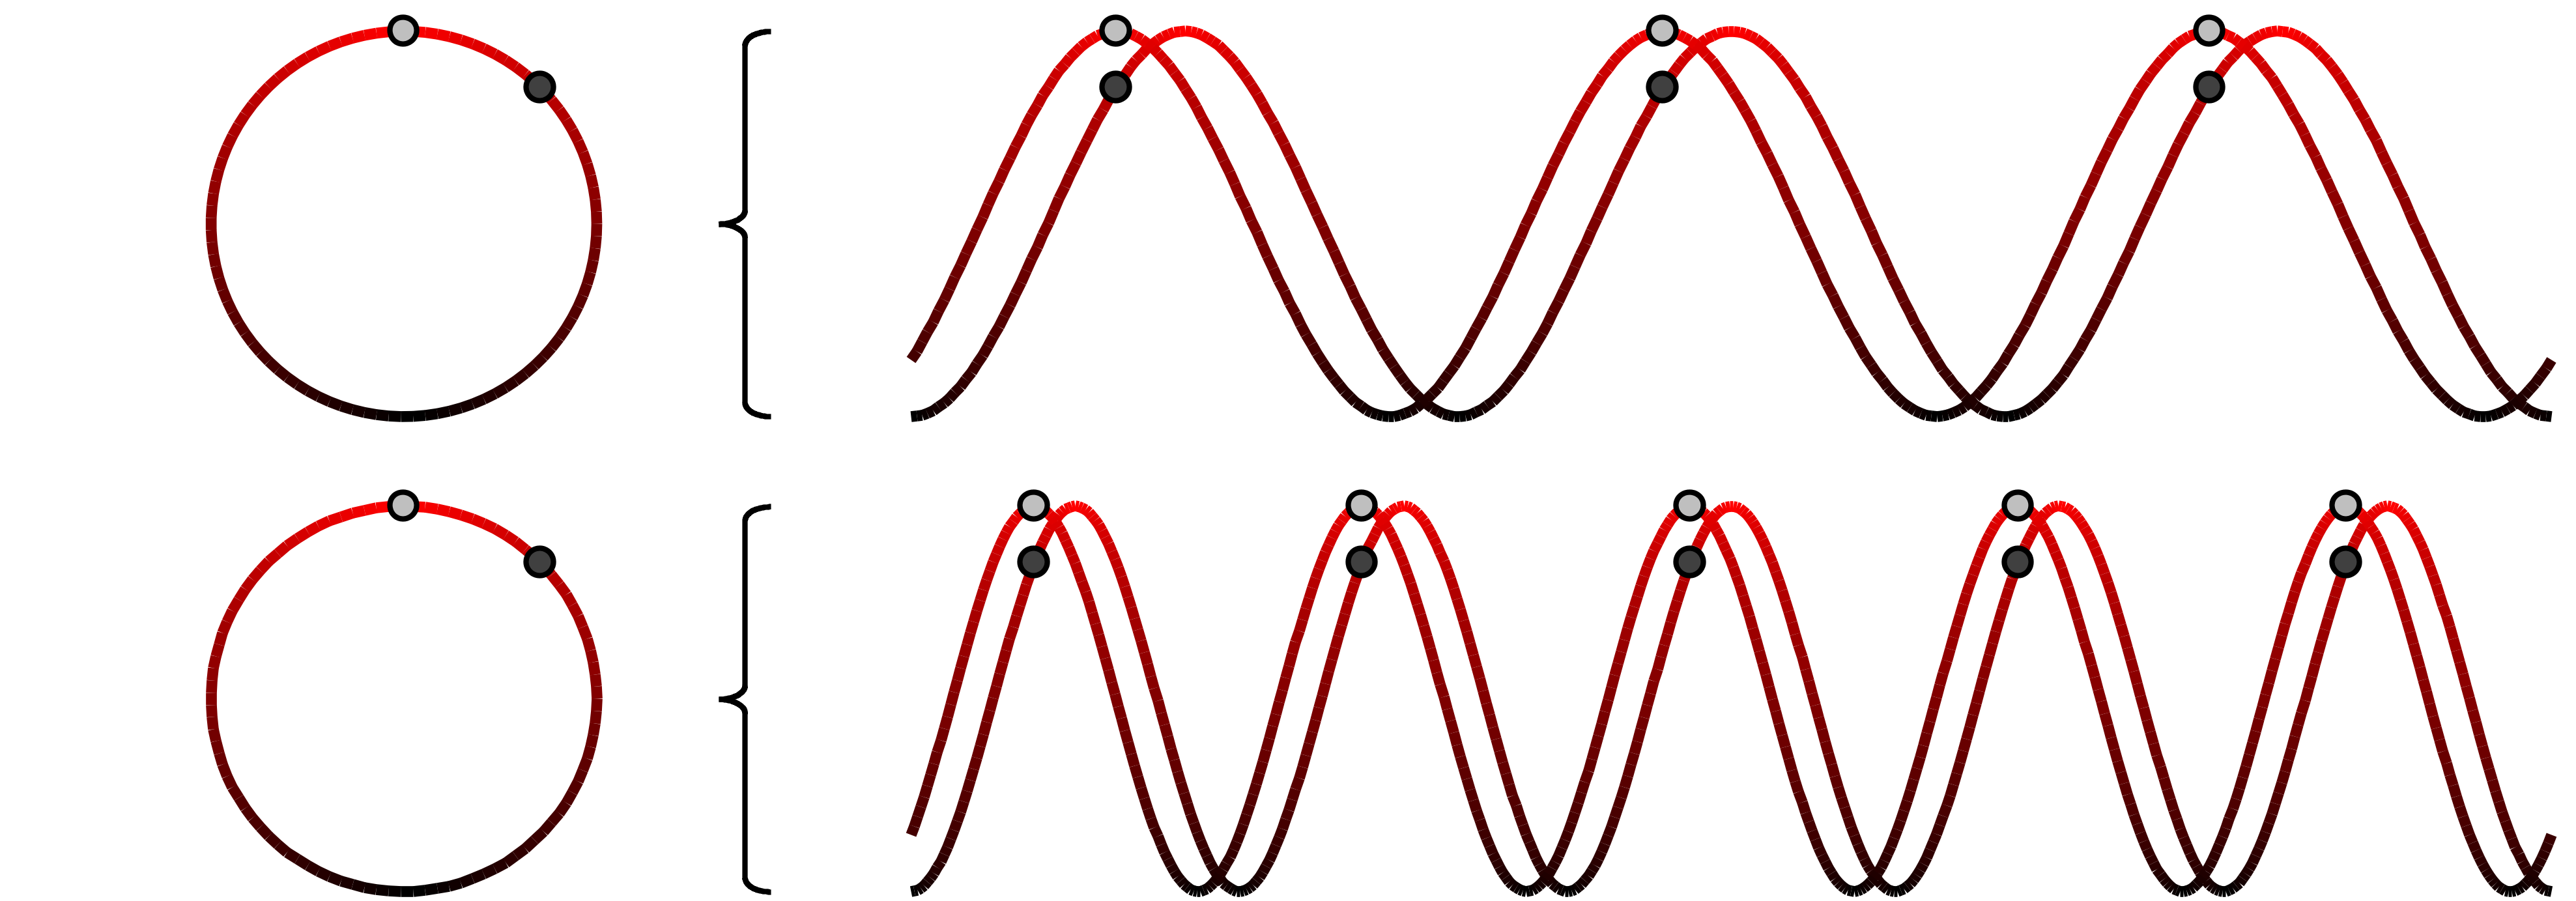
\includegraphics[width=\textwidth]{figures/Tilsen-img48.png}
\caption{\missingcaption}
\label{fig:}
\end{figure}
 

  Periodic time also allows us to see all meaning experiences as a form of symmetry breaking. Consider that an inactive population—which gives rise to no meaning experience—has continuous time reversal and translation symmetries (action potentials are uncorrelated). The emergence of a collective oscillation breaks these symmetries, but preserves a discrete/periodic translational symmetry.

\subsection{Discontinuous time}

The discontinuous time schema is a blend of a discontinuity schema with linear time. In continuous linear time, the linearity property is \textit{global}, applying at all locations in time/space. Moreover, the time/space line is continuous and infinite, extends forever in both directions, and there are no locations which are not “connected” to all other locations. In contrast, these properties do not hold for discontinuous time. By imposing a \textit{discontinuity schema} on linear time, discontinuous time separates time/space into pieces (epochs) which are disconnected from each other. Thus we expect some effective time quantities to change discontinuously “between” epochs. This is useful for conceptualizing the hypothesized reorganization mappings of the excitation operator Ê, which are so fast that they appear discontinuous on the scale in which e configurations remain stable. In a sense, discontinuous time helps us avoid worrying too much about the internal dynamics of e configuration reorganizations. Instead, we focus on stable e configurations within epochs.

  
\begin{figure}
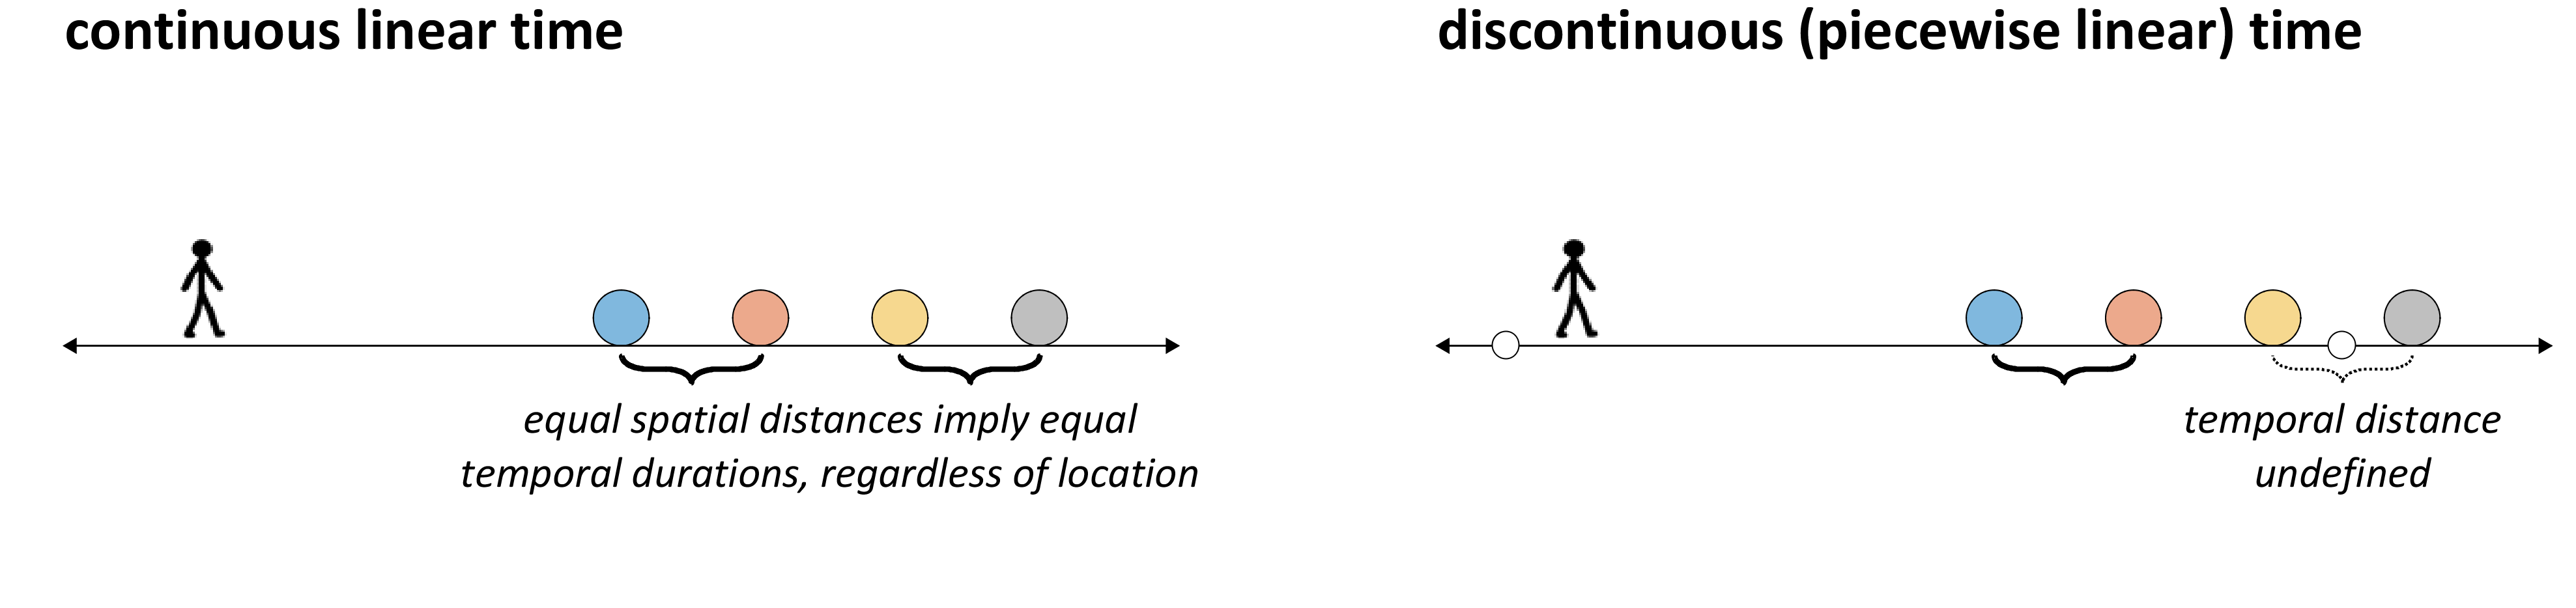
\includegraphics[width=\textwidth]{figures/Tilsen-img49.png}
\caption{\missingcaption}
\label{fig:}
\end{figure}
 

  The time-integral of the excitation state variable (\textit{e}) is an effective time quantity which exhibits discontinuities in its first derivative between stable e-epochs. Recall that the canonical e-reorganization involves demotion of a selected system and promotion of other excited systems. As shown below, the effective time quantity \textit{e} changes abruptly in the transitions between epochs, and is constant within them. Consequently there is an elbow (discontinuity in first derivative) in the time-integral of \textit{e}. This is particularly relevant when we consider that feedback mechanisms influence when reorganizations occur. Feedback may be correlated with the integral of selection-level excitation; when the integral of selection-level excitation reaches a threshold, a reorganization occurs.

  
\begin{figure}
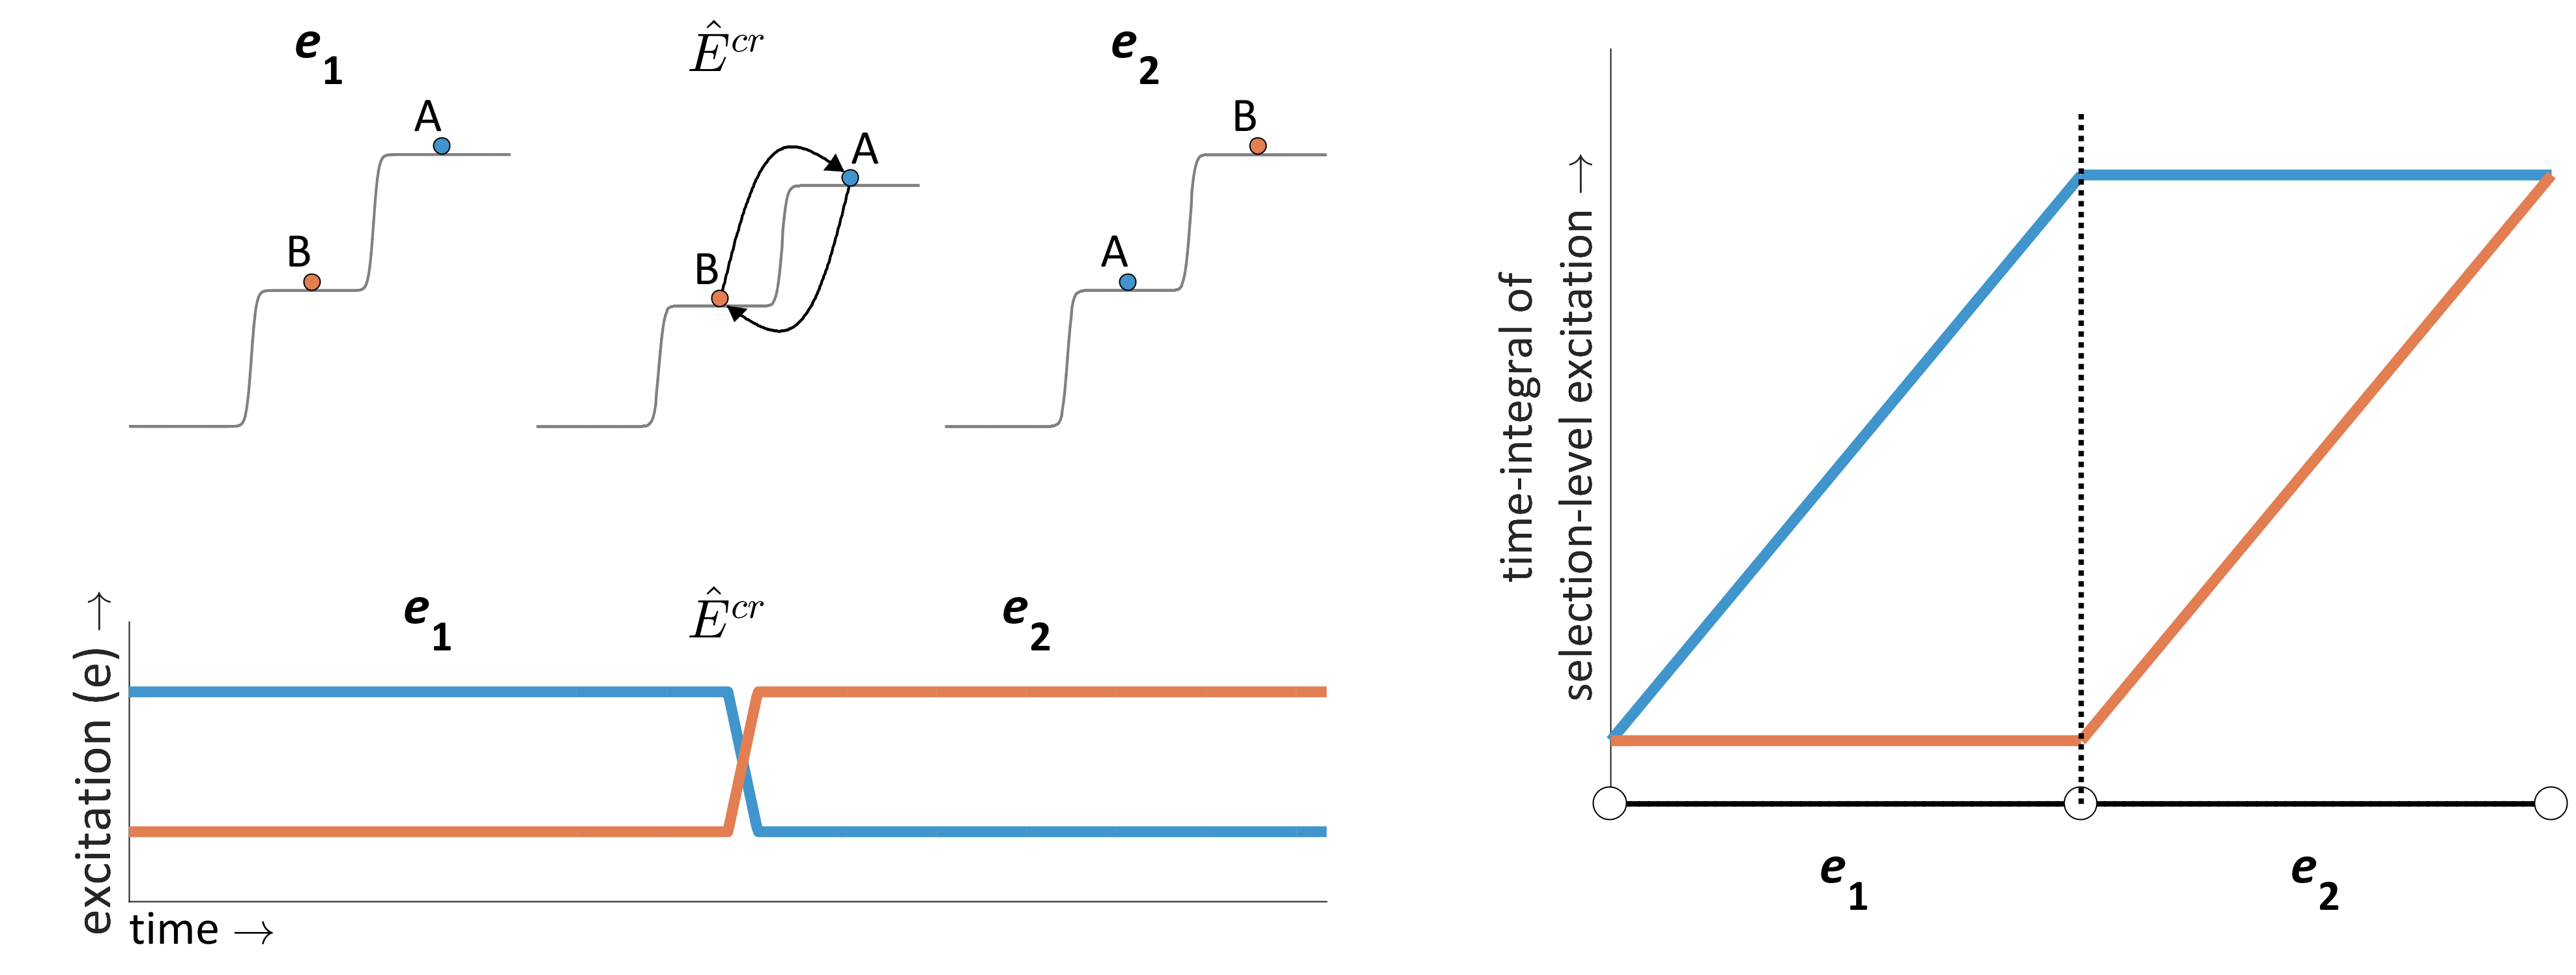
\includegraphics[width=\textwidth]{figures/Tilsen-img50.png}
\caption{\missingcaption}
\label{fig:}
\end{figure}
 

  Another reason the discontinuous time schema is useful is that we cannot readily blend it with the words-are-objects metaphor. The object metaphor evokes a static, time-invariant structure that persists throughout an utterance. The discontinuous time schema is antithetical to that sort of conception, because it does not gel with persistence across multiple e-epochs. 

  Our analyses of linguistic patterns can be improved by conceptualizing time as multiform: different conceptions of time are useful for different phenomena on different scales. This is a consequence of the inherent complexity of language: linguistic patterns arise from interactions between systems on a wide range of spatial and temporal scales; to impose a single temporal schema on a given analysis, or even worse to ignore time altogether, is a counterproductive oversimplification. 

\chapter{Reconstructing syntactic theory}

In previous chapters we introduced new conceptual tools—oscillators and energy levels—and compared them to conventional ones. We now use these tools to construct a new understanding. Our starting point is the \textit{canonical production trajectory}, which is a simplified, idealized model of the cs-state trajectory which occurs before and during the production of an utterance. The trajectory describes a situation in which a speaker is producing an utterance, rather than interpreting one. More generally, we distinguish between \textit{production}, in which state trajectories may directly give rise to motor actions by a producer (speaker/signer/writer), and \textit{interpretation}, in which the state trajectory of an interpreter (hearer/sign-viewer/reader) is driven strongly by external forces. (As we discuss later it is not always possible or even desirable to draw a clear cut distinction between production and interpretation). The trajectory we examine below is called \textit{canonical} because it is a standard trajectory which serves as comparison for other, more complicated trajectories.

\section{The canonical production trajectory}

To describe the canonical production trajectory, we use the utterance \textit{Al drinks coffee} as an example. The choice of these particular words is made for concreteness, and for various reasons a single clause without modifiers is preferable. We impose the over-simplification that there are three relevant c-systems: [Al], [drinks], and [coffee], and assume that these resonate with \{+N\}, \{V\}, and \{-N\} s-systems, respectively. We furthermore assume that the utterance is produced in a communicative context in which it is felicitous, which amounts to stipulating that peripheral sensory systems, motor systems, and previously excited or activated c-systems (i.e. the surroundings) activate the relevant c-systems and perhaps others. Under these assumptions, we divide the canonical trajectory into the following stages:

  
\begin{figure}
\includegraphics[width=\textwidth]{figures/Tilsen-img51.png}
\caption{\missingcaption}
\label{fig:}
\end{figure}
 

\subsection{{1. Forces from the surroundings activate cs-systems}} 

The surroundings activate c-systems [Al], [drinks], and [coffee]. In general, other c-systems will already be active, or may become active. There may be many such systems, e.g. [Bo], [sips], [tea], etc. All of these c-systems begin to resonate with s-systems, forming cs-systems, but in the canonical trajectory we assume the \textit{e} values of these cs-systems are initially below the excitation threshold, i.e. unexcited. Recall the distinction between the ground-level (i.e. active, unexcited) and above-ground (excited) \textit{e} states of cs-systems: systems in the excited state can participate in stable φ configurations, while unexcited systems cannot. In the initial state of the canonical trajectory, all systems are unexcited, and hence shown on the ground level of the e-potential. This does not imply that all cs-system \textit{e} values are the same, merely that we have chosen not to differentiate them. Note that in more general cases, we do not need to assume that all systems are unexcited in the initial condition.

\subsection{2. Excitation of cs-resonances}

In the pre-stable phase of production, there is a competition process, or attentional focusing mechanism, which results in some cs-systems becoming excited and others remaining unexcited, or potentially deactivating. In the present example, [Al]\{+N\}, [drinks]\{V\}, and [coffee]\{-N\} systems become excited; [Bo]\{+N\}, [sips]\{V\}, and [tea]\{-N\} deactivate. The competitive character of the mechanism is due to interference between cs-resonances. For example, as pictured below, early on in competition process \{V\} resonates with both [drinks] and [sips] c-systems. All three of these systems (i.e. [drinks], [sips], \{V\}) have some initial θ and $\theta ′$. The initial phase velocities (or more relevantly, the short-timescale averages of $\theta ′$) are not necessarily equal, partly because the intrinsic frequencies of systems are not necessarily equal, and partly because the surroundings forces on each system can vary. Furthermore, the initial phases of these systems do not necessarily conform to proximal (φ=0) or distal (φ=π) relative phase patterns. In other words, the systems are neither frequency-locked nor phase-locked, prior to being excited. Thus we expect interference: φ{}-coupling of [drinks] and \{V\} interferes with φ{}-coupling between [sips] and \{V\}.

  
\begin{figure}
\includegraphics[width=\textwidth]{figures/Tilsen-img52.png}
\caption{\missingcaption}
\label{fig:}
\end{figure}
 

  From the microscopic model we infer that φ{}-coupling force strengths depend on system \textit{e} values: the more neurons which participate in a collective oscillation, the more synaptic projections there are from that population to other ones. Thus if [drinks] has a higher \textit{e} value than [tea], it will exert stronger forces on \{V\}. This results in a greater tendency toward equalization of phase velocity between \{V\} and [drinks], compared to \{V\} and [tea]. Through e-coupling, \{V\} and [drinks] will mutually augment one another more than \{V\} and [tea]. The positive feedback loop, i.e. resonance, leads to excitation of the [drinks]\{V\} system, at the expense of [sips]\{V\}. The cs-system [drinks]\{V\} evolves toward a strong constructive interference pattern, while [sips]\{V\} experiences destructive interference.

  The outcome of resonance-focusing must be a complex function of the states of the active systems and surroundings forces. We do not attempt to model this function, but rather assert that in the canonical trajectory, some subset of active systems becomes excited; in the current example these are [Al]\{+N\}, [drinks]\{V\}, and [coffee]\{-N\}. Later on we consider deviations from the canonical trajectory in which the competition process does not immediately result in excited cs-resonances, or in which the processes is interrupted by surroundings forces.

  Why does one particular configuration of cs-systems emerge as opposed to another? For example, why does a state with excited [Al]\{+N\} and [coffee]\{-N\} systems arise, as opposed to excited [coffee]\{+N\} and [Al]\{-N\} systems (i.e. \textit{coffee drinks Al})? We assume that early in the pre-stable phase, the unexpected [Al]\{-N\} and [coffee]\{+N\} resonances are active and compete with the expected ones. Part of the reason why the expected set wins the competition may be learned asymmetries in coupling forces: c-systems with greater degrees of animacy, like [Al], are biased to resonate with the \{+N\} system, and c-systems with less animacy, like [coffee], are biased to resonate with the \{-N\} system. But learned semantic biases cannot be the whole story, since we must account for cs-resonance asymmetries in utterances such as \textit{Al sees Bo} where c-system animacies are the same. Thus we presume that information in the patterns of forces from the surroundings (i.e. sensorimotor experience) biases cs-coupling in a contextually appropriate way. For \textit{Al sees Bo}, the φ symmetry with respect to [sees]\{V\} of [Al]\{N\} and [Bo]\{N\} is broken by surroundings forces: asymmetries in how a producer experiences sensory information, e.g. aspects of the visual scene of Al seeing Bo which differ from aspects of the visual scene of Bo seeing Al, exert biases on c-system to s-system mappings in the pre-stable phase.

\subsection{3. Emergence of a stable φ configuration}

A φ configuration stabilizes due to strong φ{}-coupling forces between s-systems. φ{}-stabilization must follow excitation of the participating cs-resonances. This constraint follows from our hypothesis that cs-systems must be in the excited state in order to φ-couple strongly with other systems. The criterial/threshold \textit{e} value for excitation can be viewed as a minimal degree of order in a system which is necessary for a person to \textit{be consciously aware} of the system, an \textit{attentional threshold}, in a sense. Exactly what is meant phenomenologically by “awareness” and “attention” here, we do not attempt to elaborate. 

   Stabilization of a φ configuration is the beginning of a relational meaning experience, and in the canonical case the configuration will persist throughout the utterance. There a number of interesting questions to consider regarding meaning experience conceptualized in this way. How long must a stable φ configuration persist in order to give rise to awareness of a relational meaning? It seems reasonable to guess that in order for awareness to arise, the configuration must be maintained for a period on the order of 100s of milliseconds, but perhaps there are also circumstances in which we engage φ configurations on the order of 10s of milliseconds and of which we are not consciously aware.

  Can a relational meaning experience arise “by accident,” i.e. as a coincidence, without resulting from s-system φ-coupling? Coincidental relational meaning is a logical possibility. For example, surroundings forces may excite [Al]\{N\} and [drinks]\{V\} systems and \textit{by chance} (i.e. not through coupling of \{+N\} and \{V\}) the φ of [Al] and [drinks] could be approximately 0 or π, and the difference between their $\theta ′$ could be small. In that case, [Al] and [drinks] obtain the φ-pattern associated with agent-verb relational meaning, without having achieved this state through s-system coupling. Despite being a logical possibility, coincidental φ configurations are both unstable and highly improbable. If the intrinsic frequencies of the systems differ, their φ will wander in the absence of coupling. Even if we assume equivalent intrinsic frequencies, if we were to randomly draw the θ of two systems from uniform distributions, the likelihood that φ would be approximately 0 or π is very low. It is even less likely that φ would remain stable, because minor perturbations of $\theta ′$ from surroundings fluctuations or from the influences of other systems will alter any φ-pattern which has arisen by chance. Thus s-systems play a necessary role in stabilizing φ configurations.

\subsection{4. Emergence of a stable e configuration}

Excitation of cs-resonances necessarily precedes stabilization of φ configurations, but does φ configuration stabilization necessarily precede e configuration stabilization? In the canonical trajectory we stipulate that the e configuration stabilizes \textit{after} φ-stabilization. This is a sensible hypothesis because e configurations can depend on φ configurations. The mapping of cs-systems to e-potential levels varies substantially according to the freedom of word order in a language: in some languages, e-organization is strongly influenced by φ configuration. In languages with relatively free word order, the effects of surroundings forces on \textit{e} may have a greater influence on e-organization than learned φ-e mappings. We discuss differences between fixed and  free word order in more detail later on, but note here that e-organization is in general determined both by surroundings forces and learned φ-e mappings.

  The primacy of φ-stabilization relative to e-stabilization is also a sensible assumption for the canonical trajectory because φ-epochs (periods of time in which a φ configuration is stable) typically span multiple e-epochs (periods of time in which an e configuration is stable). In the canonical trajectory, the initial organization mapping of the excitation operator Ê may depend on φ-states, but subsequent reorganization mappings do not. For more general trajectories, we allow for e- and φ- organization mechanisms to interact in pre-stable and post-stable phase of production, and hence we expect an interplay between φ and \textit{e} states. However, in canonical production φ and \textit{e} states can interact only in the pre-stable phase; during stable epochs of canonical production, φ and \textit{e} states have no influence on one another. 

\subsection{5. Iterated reorganization of e configuration}

After the emergence of a stable e configuration, what happens next depends on the configuration itself: if the most highly excited system is above the selection threshold, then feedback processes induce the application of the canonical reorganization mapping: the selected system is demoted and others are promoted. This mapping is iterated until all systems have been selected. In contrast, if the most highly excited system is initially below the selection threshold, no reorganization occurs. Thus we distinguish between production regimes which are \textit{selective} (i.e. selection occurs) and those which are \textit{non-selective}, as shown below. Note that we represent the non-selective case by leaving the highest level of the e-potential unoccupied. For the canonical trajectory, we assume the selective regime, and hence iterated reorganization which potentially drives overt production. 

  
\begin{figure}
\includegraphics[width=\textwidth]{figures/Tilsen-img53.png}
\caption{\missingcaption}
\label{fig:}
\end{figure}
 

  The selection threshold can vary over time. This variation could be quite complicated, because the threshold represents an integration of surroundings interactions with cs-systems. For example, a speaker can be in relatively higher and lower states of physiological arousal, more or less prone to engage in simulation or execution regimes of production. Alternatively, an individual can be in a regime where they direct attention to environmental stimuli, where motor sequencing must be inhibited. Thus the dynamics of the threshold are associated with an \textit{intention} to engage conceptual-syntactic simulation, and this intention is a function of many systems. Note that we use the term \textit{selection} to refer to a non-linear gating mechanism which depends on \textit{e} values and the selection threshold. This gating mechanism controls the selection of cs-systems.

  What causes Ê to transition from the stabilizing regime to the reorganization regime in the canonical trajectory? To answer this we introduce the \textit{parallel domains} hypothesis\footnote{This hypothesis is named in honor of Jean-Roger Vernaud, who believed deeply in the necessity of developing a unified understanding of syntactic and phonological patterns (see e.g. \citealt{FreidinVergnaud2001,Vergnaud1977}); I was the lucky beneficiary of a seminar Jean-Roger and Louis Goldstein held on this topic in the fall of 2009.} , which holds that gestural-motoric organization occurs through the same mechanisms as conceptual-syntactic organization: gestural systems resonate with motoric systems, motoric systems are strongly φ-coupled attractively or repulsively, and \textit{gm-systems} are organized into a quantal relative excitation potential. Furthermore, there are strong interactions between systems in conceptual/syntactic and gestural/motoric domains: activation of a cs-system activates associated gm-systems; excitation of a cs-system augments the \textit{e} values of those active gm-systems; selection of a cs-system induces excitation of the associated gm-systems, which in the canonical trajectory leads to selection of those gm-systems. More specifically, we imagine that the selection of a cs-system induces a nonlinear boost in the excitation of the c-system; the c-system is presumed to be +e-coupled to a \textit{g-domain}, a set of g-systems. The g-domain is thereby excited and selected. Feedback from gm-states then induces the transition to the reorganization regime of  Ê.

  In the parallel domains hypothesis, articulatory gestures (\textit{g-systems}) are analogs of c-systems, and motoric systems (\textit{m-systems}) are analogs of s-systems. The interaction between domains is such that selection of cs-systems drives organization of gm-systems, and this creates states which through feedback induce reorganization of cs-systems. The interactions between domains are schematized below. Activation of gm-systems precedes and is distinct from excitation of gm-systems. In the canonical trajectory, only the gm-domains of selected cs-systems are necessarily excited. Feedback regarding the achievement of a gm-state induces reorganization of cs-systems, which in turn leads to a new gm-organization and more feedback, etc.

  
\begin{figure}
\includegraphics[width=\textwidth]{figures/Tilsen-img54.png}
\caption{\missingcaption}
\label{fig:}
\end{figure}
 

  A specific example is shown below (for expository purposes we substitute \textit{Alexi} for \textit{Al}). When [Alexi]\{N\} is selected (A), the g-systems associated with \textit{Alexi} resonate with m-systems and gm-systems become excited (A\textsubscript{1}). The particular φ/e-organization that arises is partly learned (lexically driven) and partly influenced by “post-lexical” phonological processes (e.g. resyllabification). Note that in the depiction of gm-system e-organization, the gm-systems associated with each syllable occupy a different level. Here we use segmental labels for gm-systems out of convenience but a more useful analysis would depict gestures (i.e. bilabial closure, glottal adduction, etc., which are possibly the smallest scale of organization in premotor cortex). In a canonical trajectory, the most highly excited set of gm-systems is above the selection threshold, and this de-gates the execution of movements associated with the relevant g-systems. The precise timing of execution of co-selected gm-systems is determined by the relative phases and frequencies of those gm-systems (i.e. coordinative control, as described in Selection-coordination theory, cf. \citealt{Tilsen2016,Tilsen2018}). 

  
\begin{figure}
\includegraphics[width=\textwidth]{figures/Tilsen-img55.png}
\caption{\missingcaption}
\label{fig:}
\end{figure}
 

  For adult speakers in normal circumstances, internal (i.e. predictive/anticipatory) feedback regarding achievement of articulatory targets leads to promotion of non-selected gm-systems and suppression of the selected set of systems (A\textsubscript{2}). The newly selected set is executed, internal feedback induces degating and suppression, leading to the gm-state in (A\textsubscript{3}). When all sets have been selected and suppressed, feedback regarding the gm-state associated with [Alexi] induces reorganization to the cs-state in (B), i.e. demotion of [Alexi]\{N\} and promotion of [drinks]\{V\}. When [drinks]\{V\} is selected, the g-domain of [drinks] is e-organized and executed (B\textsubscript{1}). Feedback leads to the s-system reorganization in (C), which leads to organization and reorganization of the gm-domain of [coffee] (C\textsubscript{1} and C\textsubscript{2}).

\subsection{6. The surroundings drive the system to a new state}

The φ-epoch in which [Al]\{+N\}, [drinks]\{V\}, and [coffee]\{-N\} are excited comes to an end. The state trajectory will change drastically, depending sensitively on the surroundings and other c-systems. Hence we make no assumptions about the subsequent state in the canonical production trajectory. We imagine that excitation of [Al], [drinks], and [coffee] c-systems may activate (“prime”) semantically associated c-systems through weak e-coupling. This priming comes in the form of biasing forces on the state trajectory, with numerous other surroundings forces determining the outcome. It is important to note that our representations depict only the most strongly excited (above-ground) systems, only the tip of an iceberg. In a more detailed analysis, many more cs-systems and gm-systems would be active throughout the trajectory. Various environmental/contextual factors—is it a socially appropriate time to speak?, are there salient environmental forces acting on a speaker?—along with the current system state, influence the evolution of the system. 

\section{Interactions between conceptual-syntactic and gestural-motoric organization}

The o/el framework aims to provide a \textit{comprehensive} framework for analysis of language, a theory that can describe any empirical phenomenon. Our primary focus in this book is on conceptual-syntactic organization, rather than gestural-motoric organization. However, there are a number of hypotheses regarding gestural-motor organization and its interaction with conceptual-syntactic organization, which are worth discussing here.

\subsection{Similarities between relational meaning and temporal coordination}

One deep consequence of the parallel domains hypothesis is that two superficially distinct phenomena—relational meaning and precision control of movement execution—arise from the same mechanism. The principle of relational meaning corresponds to a principle of gestural coordination. Specifically this shared mechanism is φ-coupling between syntactic systems and between motoric systems, which indirectly brings about a φ configuration between conceptual and gestural systems, respectively. Distinctions such as agent/patient (\{+N\}, \{-N\}) and onset/coda (\{+C\}, \{-C\}) are analogous, since agents and onsets experience +φ (attractive) forces from \{V\} and vowels, while patients and codas experience -φ (repulsive) forces from \{V\} and vowels. This speaks to a deep connection between our experience of meaning and coordination of movement. The need to flexibly coordinate a fairly small set of movements is an evolutionarily ancient problem, while the need to flexibly relate a vast multitude of concepts is relatively more modern. Our ability to experience a wide variety of relational meanings probably originates from duplication-induced redundancy and functional divergence in the neural systems that support φ-coupling of movement tasks. 

\subsection{Differences between syntactic and motoric sequencing} 

Although there are deep similarities between cs- and gm-organization, there are also some important differences: 

\begin{enumerate}
\item \textit{m-system} φ configuration\textit{al restriction}. Whereas s-system φ configurations can arise between systems which occupy different e-levels, m-system φ configurations tend to arise only for co-selected gm-systems, i.e. m-systems which occupy the same level. 

\item \textit{gm-interference is more stable than cs-interference}. Both c- and g- systems can interfere with other c- and g- systems, when resonating with the same s- and m- systems. However, gm-resonances appear to interfere with one another to a lesser extent. For instance, it is possible to have a stable configuration of three co-selected \{+C\} and \{-C\} constriction gestures, as in the word \textit{sprints}. In contrast, lexical s-systems like \{+N\}, \{-N\}, and \{V\} are never co-selected. This suggests that \{+C\} and \{-C\} differentiations of gm-systems which have similar \textit{e} values can be accomplished without destabilization. We note that the ability to organize multiple gm-differentiations of \{+C\} or \{-C\} systems must be learned, and many languages lack the complex syllable structures which require such differentiations.

\item \textit{c-system numerosity}. c-systems are vastly more numerous and diverse than g-systems. This is likely because g-systems interact more broadly with motor and sensory physiology. Practical considerations dictate that we construct c-systems in an analysis-specific way, because there are potentially so many of them. In contrast, we can often identify an constant set of g-systems for analyses of a given language (at least on supra-utterance scales), which is motivated  by articulatory and acoustic observations.

\item  \textit{Timescale of} φ \textit{configuration.} s-system φ configurations persist and remain stable over relatively longer periods of time than m-system φ configurations. In the cs domain, φ configurations tend to persist over multiple reorganizations of e configurations; in the gm domain, φ configurations tend to be associated with just one cs domain e-epoch.
\end{enumerate}

  Differences between syntactic and phonological patterns should be derivable from differences in cs- and gm-organization, such as those listed above. For example, the apparently greater degree of “non-locality” of conceptual relations vs. gestural relations may be a consequence of differences in configurational restrictions and relevant timescales. (Locality differences are not, of course, structural distances, because we do not conceptualize language as spatial ordering of objects in a linear space.) Differences between cs- and gm-organization should in turn be derivable from neurophysiological differences in the relevant neural populations.

\subsection{Thresholding for simulation and execution}

The hypothesized interaction between cs- and gm-domains involves three gating mechanisms,\footnote{A sensible pursuit in this context would be to associate the gating mechanisms/thresholds with neuro-behaviorally inspired inhibitory mechanisms \citep{DuqueEtAl2017,DuqueEtAl2010,%twice
,DuqueIvry2009,MayrEtAl2006}), but I have not attempted to explore this association in any detail.} which are associated with three thresholds: an s-selection threshold, an m-selection threshold, and an execution threshold. The states of these thresholds—which we call \textit{gates}—relative to the states of the relevant cs- and gm-systems, determines a \textit{production regime}, i.e. a class of state trajectories. 

  A threshold/gate should be viewed as an analytical simplification of forces which exhibit a nonlinear dependence on \textit{e} value. Each gate can be in a binary state: \textit{open} or \textit{closed}, where \textit{open} refers to any state in which \textit{e} values of relevant systems are below a threshold parameter value. If the states of all three gates are independent, there are 2\textsuperscript{3} = 8 distinct gate configurations. Alternatively, the gating mechanisms may be hierarchically organized, such that the highest closed gate determines the production regime; in that case there are only 4 distinct regimes. The {\figurebelow} labels the production regimes associated with a hierarchically organized interaction between gates.

  
\begin{figure}
\includegraphics[width=\textwidth]{figures/Tilsen-img56.png}
\caption{\missingcaption}
\label{fig:}
\end{figure}
 
\begin{enumerate}
\item \textit{non-simulative} regime: the s-system selection threshold (\textit{s-gate}) is closed. Relational meaning experiences can arise, but no cs-selection occurs. This regime may be associated with “non-verbal” thought. It is difficult to characterize what sorts of behaviors this regime is associated with, because there is by definition no verbal motor behavior that can be observed, without cs-selection. 

\item \textit{cs-simulation} regime: the s-gate is open, but the m-system selection threshold (\textit{m-gate}) is closed. Because the s-gate is open, highly excited s-systems can be selected, and this causes gm-resonances to be excited. s-system e configurations can be reorganized in the canonical way, driven by feedback. Yet because the m-gate is closed, motor commands are not generated and hence movements are not simulated. 

\item \textit{gm-simulation} regime: s- and m-gates are open,  but a global motor execution gate (\textit{exec-gate}) is closed. Motor commands and internal sensory feedback from movement are generated, but movements are not executed. We identify the gm-simulation regime with subvocal rehearsal and silent/covert speech. 

\item \textit{execution} regime: s-, m-, and exec-gates are open, overt speech can occur. More generally, verbal motor behaviors can arise: speaking, signing, handwriting, typing.
\end{enumerate}

  Do other production regimes occur, which could  be derived from non-hierarchical gate interactions? There are four possibilities. One is when the s-gate is closed but m- and exec-gates are open; this regime may be associated with behaviors such as filled pauses and floor holding, i.e. motor actions which are not necessarily driven by cs-resonances. Whether the remaining three possible combinations correspond to identifiable production regimes is unclear. It seems reasonable to infer that when m-gates are closed, no speech-related motor behaviors occur and exec-gate states are irrelevant to classification of production regimes.

\subsection{The roles of internal and external feedback in e configuration reorganization}

Reorganization of both cs and gm e configurations is driven by sensory feedback. We assume there are parallel feedback mechanisms for cs and gm states, and that these are associated with both internal and external feedback loops. There is a substantial literature based on the distinction between internal and external feedback when applied to motor control and speech (\citealt{Hickok2012,Kawato1999,MiallWolpert1996,RamanarayananEtAl2016,WolpertEtAl1995,WolpertKawato1998}); this distinction can be extended to higher levels of linguistic processing as well (\citealt{HagoortLevelt2009,Laver1973,Levelt1983,Levelt1989,Nooteboom1973,NooteboomQuené2008,Postma2000}).

  External feedback is sensory information regarding the state of the environment. The “environment” here is the physical state of the world: movement leads to changes in the state of the environment, e.g. in spatiotemporal acoustic energy distributions, articulator positions, muscle stretch, etc. These changes influence the states of various peripheral sensory systems, providing various forms of information, i.e. auditory, tactile, proprioceptive, etc. This information in turn influences the states of g-sensory systems, which we imagine are populations which integrate sensory information. In general, this external feedback can result in adjustments of motor commands, suppression of selected m-systems, and degating of subthreshold m-systems. However, a fairly long time delay exists between when movement occurs and when external sensory feedback associated with movement becomes available. This delay makes external sensory feedback relatively less useful for online control of movement, compared to internal feedback. 

  Internal sensory feedback is sensory information “predicted” by the nervous system, regarding the state of the environment. The prediction comes from an \textit{internal model}, which maps outgoing motor commands to sensory states. A so-called \textit{efference copy} of motor commands (or better, a motor state) is mapped to a representation of the anticipated sensory consequences those commands. Because of its anticipatory nature, internal feedback is useful for adjusting motor commands and reorganizing gm-system during execution. It is worth noting that “prediction” implies agency, and the nervous system is only metaphorically agentive. Thus it is more appropriate to describe internal feedback as follows: motor states induce sensory states, and these states are similar to ones that are induced a bit later via sensory information from the external environment.

The distinction between internal and external feedback is schematized below. In the gm-domain, internal feedback can lead to suppression (demotion) and/or degating (promotion) of systems \textit{before} external sensory feedback regarding target achievement has been received. Internal gm-feedback can also drive promotion and demotion of cs-systems in the cs-domain, via c-sensory systems. Thus internal feedback can be viewed as a general mechanism for influencing the timing of e-reorganization.

  
\begin{figure}
\includegraphics[width=\textwidth]{figures/Tilsen-img57.png}
\caption{\missingcaption}
\label{fig:}
\end{figure}
       

  To what extent are internal and external feedback involved in cs- and gm- reorganization? The answer can depend on many factors. First, because internal models (which map motor states to expected sensory states) are learned, young children must rely on external feedback to a greater degree. This is consistent with the observations that young children speak more slowly and produce syntactically simpler utterances. Second, the relative influence of internal vs. external feedback must depend on a production regime, i.e. on threshold states. For example, when exec-gates are closed, as in motor simulation, no external sensory feedback is available. Hence internal feedback is the sole mechanism for driving e-reorganization in subvocal rehearsal. Third, environmental circumstances which induce mismatches between internal predictions and external feedback can induce greater reliance on external feedback. In sensory perturbation paradigms (e.g. speech in noise, spectrally altered auditory feedback, mechanical perturbation of movement), speakers often slow down and compensate for the alteration. These behaviors are presumably a consequence of detection of a mismatch between internal predictions and external information; when such mismatches are detected, the system can no longer rely on the accuracy of the prediction, and reverts to reliance on the external information. Fourth, various contextual forces may induce speakers to attend more or less closely to their own productions, resulting in varying degrees of reliance on external feedback.

\subsection{Disfluencies}

Abnormalities in trajectories of conceptual-syntactic and gestural-motoric systems can be understood by considering the ways in which interactions between φ/e-organization, thresholds, and feedback can deviate from those associated with the canonical production trajectory. These deviations predict a typology of disfluency/speech error mechanisms which differs from standard classifications (see \citealt{Fromkin1971,Fromkin1984,Shriberg2001}). To develop this typology we distinguish between (i) disfluency manifestations, (ii) disfluency mechanisms, and (iii) disfluency origins. Manifestations are observable abnormalities in production, whereas mechanisms are hypothesized deviations from the canonical trajectory which result in a disfluency manifestation. The origins of these deviations are surroundings forces and we have little to say about them—there are numerous possibilities for why a particular deviation occurs and we rarely have a solid basis for determining them. 

  The aim of constructing a disfluency typology is to map between mechanisms and manifestations, but this is complicated because the relation is not expected to be one-to-one. In particular, some classes of manifestation may arise from more than one mechanism. For example, there may be multiple abnormal cs-trajectories which converge to the same abnormal gm-trajectory. 

  Another complication is that the initial construction of what constitutes an abnormality must presuppose a canonical \textit{intended} or \textit{target} trajectory. We often assume that there was some utterance a speaker intended to produce, that something went wrong, and that the speaker produced something else. It may not be appropriate to impose these assumptions in many circumstances. In an empirical context, the implied target trajectory is always an analytical guess: we observe some manifestation(s) of disfluency, and based on our familiarity with language, our expectations, and our notions of similarity, we guess a target utterance.

  Lets consider an example. Imagine that a speaker says \textit{Al krinks coffee}. Our analysis of \textit{Al krinks coffee} must be conducted in relation to a canonical trajectory, the target of which we guess is \textit{Al drinks coffee}. The manifestation of the disfluency is the execution of a velar closure for [k] as opposed to an alveolar one for [d]. The mechanism, as shown below in (B1), is that a velar closure, [k], obtains an above-ground gm-resonance when [drinks]\{V\} is selected, instead of an alveolar closure, [d]. We might further elaborate the mechanism by speculating that the substitution of [k] for [d] arose from a trajectory in which [k] in the domain of [coffee] outcompeted [d] for resonance with \{+C\} in (B1). Note that no \textsc{units}\textsc{{}-are-}\textsc{objects} or word order blend are imposed on this analysis of substitution: there is no sense in which [k] and [d] occupy temporal positions or move. Rather, substitutions are trajectories which, for indeterminate reasons, deviate from a canonical trajectory. 

  
\begin{figure}
\includegraphics[width=\textwidth]{figures/Tilsen-img58.png}
\caption{\missingcaption}
\label{fig:}
\end{figure}
 

  However, even the above analysis of the disfluency mechanism as noncanonical competition is merely a guess. An alternative possibility is that some other cs-resonance we have not identified was active in epoch (B), and the g-domain of this unidentified system played a role. For example, a [cold] c-system might have been active throughout the utterance, as shown below. Despite being active, [cold] is never selected because it is unexcited. Nonetheless, systems in its g-domain are active and may, with help from other forces, become excited, which constitutes a deviation from the canonical trajectory.

  
\begin{figure}
\includegraphics[width=\textwidth]{figures/Tilsen-img59.png}
\caption{\missingcaption}
\label{fig:}
\end{figure}
 

  If we allow for noncanonical reorganizations, there are even more possible analyses of disfluency mechanisms. For example, perhaps in epoch (e1) [craves]\{V\} was excited and [drinks]\{V\} unexcited, but surroundings forces caused a noncanonical reorganization to (e2), where [drinks]\{V\} is promoted to the selection level and [craves]\{V\} is grounded. Suppose the noncanonical reorganization interrupts execution of gm-systems. Such a trajectory might arise when competition between [craves] and [drinks] for \{V\} resonance continues after the initial organization and transition to a selective regime. 

  
\begin{figure}
\includegraphics[width=\textwidth]{figures/Tilsen-img60.png}
\caption{\missingcaption}
\label{fig:}
\end{figure}
 

  The above example illustrates why the notion of an intended canonical utterance/trajectory is problematic. What is the intended trajectory? Perhaps we might conduct the analysis with reference to two canonical trajectories, associated with \textit{Al craves coffee} and \textit{Al drinks coffee}. In some sense, both of these are the “intention” of the speaker. But in another sense, neither is an “intention”: the “intention” of the speaker was to change the trajectory from the one expected in (e1) to the one in (e2). Hence we might allow for the surroundings forces which cause the disfluency to be construed as intention. There are many disfluency manifestations which provide very little certainty regarding an intended trajectory. Thus rather than classifying observed disfluencies by guessing intentions, an alternative viable strategy for typologizing disfluencies is to classify ways in which perturbations of a canonical trajectory can map to manifestations.

  For a different example of disfluency, consider the utterance \textit{Al drinks…drinks coffee}, where the speaker hesitates after the first production of \textit{drinks} and repeats \textit{drinks}. Perhaps a c-system such as [tea] competes with [coffee] for cs-resonance with \{-N\}, and perhaps both [tea] and [coffee] are excited in the initial e-organization (e1). Because of this circumstance, reorganization from (e2) to (e3) fails to promote either [tea]\{-N\} or [coffee]\{-N\} to selection level. Instead, there is a period of time in which no cs-system is selected (a hesitation), while the [coffee]-[tea] competition is resolved by grounding [tea]\{-N\}. Eventually, a noncanonical reorganization to (e4) occurs, which promotes [drinks]\{V\} to selection level a second time. 

  
\begin{figure}
\includegraphics[width=\textwidth]{figures/Tilsen-img61.png}
\caption{\missingcaption}
\label{fig:}
\end{figure}
 

  By considering other noncanonical reorganizations, we can generate alternative manifestations. If the post-hesitation reorganization promotes both [Al]\{+N\} and [drinks]\{V\}, the utterance would be \textit{Al drinks…Al drinks coffee}. If the reorganization promotes no cs-systems, the utterance would be \textit{Al drinks…coffee}. If detection of the promotion failure closes s-gates temporarily, perhaps an [uh] gm-system is selected during the hesitation, and the utterance is \textit{Al drinks…uh…coffee}.

  Another example of disfluency involves a mechanism in which external feedback does not match a conceptual state—a self-monitoring disfluency. Consider the utterance \textit{Al drinks tea…coffee.} We might imagine that the utterance is produced in accordance with an canonical trajectory for \textit{Al drinks tea} (e1-e3), but for whatever reason, the speaker transitions between (e3) and (e4) to attending to an {\textbar}Al drinks coffee{\textbar} φ configuration instead of {\textbar}Al drinks tea{\textbar}. As a consequence, external feedback of [tea] is not consistent with the φ configuration which involves [coffee]; this leads to a reorganization which promotes [coffee] to selection level.

  
\begin{figure}
\includegraphics[width=\textwidth]{figures/Tilsen-img62.png}
\caption{\missingcaption}
\label{fig:}
\end{figure}
 

  By systematically analyzing ways in which production trajectories can deviate from canonical ones, and comparing these to observed manifestations, it should be possible to gain greater insight into constraints on the reorganization operator, Ê. This sort of approach also usefully structures our analysis of observed disfluencies, by compelling us to be more aware of the our assumptions regarding speaker intentions.

\subsection{Accentual and metrical patterns}

One pervasive form of cs-gm interaction involves accentual patterns such as primary stress or lexical pitch accent. In some languages, we hypothesize a class of \textit{accentual} g-systems which resonate with an accentual m-system, \{A\}. Accentual g-systems often involve tones (or pitch accents), such as [H*]. Consider the accentual pattern on the phrase \textit{Mr}. \textit{Mississippi}, as shown below. Following our previous analyses, we might conceptualize the gm-system [H*]\{A\} as the gm-domain of an accentual [\textsc{accent}]\{A\} cs-system. In other words, we could posit a class of accentual c-systems [\textsc{accent}] and a corresponding class of s-systems, \{A\}. However, there are some problems with this analysis. In many cases the participation of the [\textsc{accent}]\{A\} system in a relational meaning experience is hard to characterize. Moreover, we have no reason to suspect that [\textsc{accent}]\{A\} needs be reorganized like other cs-systems, because all selective epochs can include selection of [\textsc{accent}]\{A\}, and many stress/pitch accent languages have a default gm-domain for [\textsc{accent}].

  
\begin{figure}
\includegraphics[width=\textwidth]{figures/Tilsen-img63.png}
\caption{\missingcaption}
\label{fig:}
\end{figure}
 

  Indeed, the observation that an accentual system can be selected once in each epoch, regardless of which other cs-systems are selected, suggests that we view the accentuation system differently. The alternative we pursue is to posit a special accentual s-system \{\^{}\}. The s-system \{\^{}\} does not differentiate like other s-systems; instead \{\^{}\} is selected and re-selected in each selective epoch and potentially excites the gm-domain of an accentual c-system, i.e. [\textsc{accent}], without necessarily φ-coupling to that c-system. In the case of intonational accents, we imagine that different varieties of [\textsc{accent}] c-systems (e.g. [\textsc{contrast}], [\textsc{focus}], [\textsc{surprise}]) may couple to lexical s-systems, and that \{\^{}\} excites the gm-domains of those [\textsc{accent}] c-systems. In the absence of a more specific c-system being excited, a default gm-domain may be excited by \{\^{}\}. This circumstance accounts for the typological pattern of \textit{stress}, where each set of co-selected cs-systems is produced with one primary accent. This could be a default gm-system or a more pragmatically meaningful one that is the domain of [\textsc{contrast}], [\textsc{focus}], etc. For patterns called \textit{pitch accent}, the gm-domain of \{\^{}\} can be determined by the co-selected cs-system.

  The metrical organization of accentual gm-systems relates to how the m-system \{A\} is organized in a multi-level gm-domain. For example, the gm-configuration of \textit{Mississippi} has four e-levels, and \{A\} initially occupies the third e-level. In some languages the organization of \{A\} is determined entirely by the number of e-levels in the gm-domain (fixed stress). In other languages the organization of \{A\} can be influenced by the identity of the selected cs-system (free stress). In both cases, the compositions of the gm-systems may influence \{A\} organization (quantity sensitivity). 

  To account for secondary stress in the gm-domain of co-selected cs-systems, we hypothesize that gm-configuration re-organization can be driven by rhythmic m-system selection. As shown below, co-selected \{+C\}\{V\} m-systems are +φ-coupled. Constructive interference between m-systems occupying different e-levels is maximized when oscillation phases align. We can associate the maximized constructive interference pattern with \textit{periodic e-reorganization} and an reorganization frequency, \textit{f}\textsuperscript{0}. Periodic reorganization occurs when there is a periodicity which strongly influences the timing of promotion and demotion (i.e. the canonical reorganization regime). Importantly, periodic reorganization is not a general mechanism of conversational speech. Instead, it is a regime associated with specialized contexts, e.g. poetic meter/rhythmic speech, entrainment to external stimuli, and analytical reflection on metrical patterns—i.e. metrical intuition formation. Periodic reorganization may also be a developmental mechanism for stabilizing e-reorganization processes, as in babbling. In disfluency and some disordered speech, it may emerge as a stabilizing mechanism.

  
\begin{figure}
\includegraphics[width=\textwidth]{figures/Tilsen-img64.png}
\caption{\missingcaption}
\label{fig:}
\end{figure}
 

  To reconceptualize higher-level prosodic organization, we hypothesize that the maximized constructive interference pattern facilitates the emergence of subharmonic oscillations at frequencies \textit{f}\textsuperscript{{}-1}, \textit{f}\textsuperscript{{}-2},… \textit{f}\textsuperscript{{}-n} and that cs-systems can φ-couple to these subharmonics via coupling of generalized relative phase, i.e. φ\textsubscript{ij} = 2π(\textit{f}\textsubscript{j}θ\textsubscript{i} - \textit{f}\textsubscript{j}θ\textsubscript{i}). If subharmonic oscillations are influential during a developmental stage in which rhythmic e-reorganization is a heuristic/bootstrapping mechanism, speakers might learn to +φ-couple \{A\} m-systems with the lowest subharmonic oscillation.

\section{Morphosyntax and morphophonology}
\subsection{Grammatical vs. lexical systems}

Up to this point, our analyses have focused on \textit{lexical} cs-systems. For example, we have ignored the fact that the word \textit{drinks} in \textit{Al drinks coffee} is associated with grammatical person and number. We can elaborate our analyses by including state space dimensions for \textit{grammatical} cs-systems, i.e. systems which evoke so-called \textit{functional} or \textit{grammatical} meaning, e.g. tense, aspect, mood, voice, person, number, gender, case, definiteness, etc. A variety of differences between grammatical and lexical systems are enumerated below. However, one should infer no \textit{essential} distinction between these types of systems; “grammatical system” and “lexical system” are analytical categories, which have more or less prototypical members and heterogeneous category structure. On historical scales, more prototypically grammatical systems tend to evolve from more prototypically lexical ones, and hence we expect intermediate varieties and cases in which different types of cs-systems are associated with the same or similar gm-domains. 
\begin{enumerate}

\item Grammatical c-systems resonate with grammatical s-systems through +φ-coupling, just like lexical c-systems resonate with lexical s-systems such as \{N\}, \{V\}, \{Adj\}, \{Adv\}. We construct various types of grammatical s-systems for various types of grammatical c-systems. Hence to understand how a concept of 3\textsuperscript{rd} person is evoked in a relational meaning experience, we construct a [3\textsuperscript{rd}] c-system, an s-system \{\textsc{person}\}, and a cs-resonance [3\textsuperscript{rd}]\{\textsc{person}\}. 

\item Like lexical cs-resonances, grammatical cs-resonances are canonically one-to-one, i.e. a grammatical c-system will strongly resonate with only one grammatical s-system in a local epoch, and vice versa. The reason for this is interference: before φ-stabilization, c- and s- systems will generally have different angular velocities $\theta ′$ and phases θ. This makes configurations with many-to-one resonances unstable (we examine interference in more detail, later in this chapter).

\item Lexical and grammatical c-system networks exhibit a variety of differences. Grammatical c-systems which resonate with the same class of s-system exert relatively strong inhibitory forces on each other, while lexical c-systems exert relatively weak inhibitory forces. To elaborate the intuition behind this, lets assume that for each s-system we can identify a \textit{c-domain} as the set of all c-systems which may resonate with the s-system. Hence the c-domain of \{\textsc{person}\} is [\textsc{1}\textsc{\textsuperscript{st}}], [\textsc{2}\textsc{\textsuperscript{nd}}], [\textsc{3}\textsc{\textsuperscript{rd}}]. The c-domain of a lexical s-system such as \{V\} has many more c-systems in its c-domain than \{\textsc{person}\} does. Imagine these networks of interactions between c-systems as below. Our intuition is that grammatical c-domain networks are fully connected and have relatively strong, inhibitory e-coupling forces between all systems, whereas lexical c-domain networks are sparsely connected with relatively weak e-coupling, which may be of either negative (-e) or positive (+e) valence.

  
\begin{figure}
\includegraphics[width=\textwidth]{figures/Tilsen-img65.png}
\caption{\missingcaption}
\label{fig:}
\end{figure}
 

\item On supra-utterance scales, there are statistical differences in how often grammatical and lexical cs-systems are excited: typical grammatical cs-systems are excited more frequently than lexical ones. The greater occurrence frequency correlates with differences in c-domain network structure, and this should be derivable from a microscopic model. The difference between +e and -e coupling derives from the relative proportion of postsynaptic targets of projections between populations: projections from excitatory neurons in one population to excitatory neurons in the other population promote +e coupling; projections to inhibitory interneurons promote -e coupling. The numbers of such projections between any two populations, along with their synaptic weights, is influenced on supra-utterances scales by learning mechanisms such as spike-timing dependent plasticity. The macroscale consequence is that in grammatical c-domains, because of the greater occurrence frequency of grammatical cs-resonances, c-systems evolve to exert and experience stronger e-coupling forces on other grammatical c-systems, compared to lexical c-domain networks. Hence our microscale conceptualization predicts a correlation between occurrence frequency and within-domain connectivity/coupling strengths.

\item  In order for a grammatical cs-system to participate in a relational meaning experience, the grammatical s-system must φ-couple with a lexical s-system. The valence of this coupling is always +φ. For \textit{Al drinks the coffee} shown below, this entails that \{\textsc{person}\} and \{\textsc{number}\} are +φ coupled to \{V\}, and \{D\} is +φ coupled to \{-N\}. Consequently [\textsc{3}\textsc{\textsuperscript{rd}}] and [\textsc{sg}.] have a +φ relation to [drink], and [\textsc{definite}] has +φ relation to \{-N\}.

\item Grammatical s-systems are often organized in the same e-level as the lexical s-system they are φ-coupled to. An example is shown below, where [3\textsuperscript{rd}]\{\textsc{person}\} and [\textsc{sg.}]\{\textsc{number}\} are on the same level as [drink]\{V\}, and [\textsc{def}.]\{D\} is on the same level as [coffee]\{-N\}. This entails that \{\textsc{person}\}, \{\textsc{number}\}, and \{V\} are co-selected, and that \{D\} and \{-N\} are co-selected. Although lexical s-systems are not co-selected with other lexical s-systems, grammatical s-systems can be co-selected with other s-systems, lexical and grammatical. A compound lexical system is normally organized as one cs-system, i.e. [coffee-stain]\{N\}, as opposed to two independently selected systems.

  
\begin{figure}
\includegraphics[width=\textwidth]{figures/Tilsen-img66.png}
\caption{\missingcaption}
\label{fig:}
\end{figure}
 

\item  Grammatical s-systems are associated with a greater degree of population differentiation, particularly in highly inflected languages. In cases where subject nouns, object nouns, and verbs are inflected for some grammatical meaning, we analyze each inflectional marking as a distinct cs-resonance arising with differentiated grammatical s-systems. In the same way that the \{N\} population differentiates into \{-N\} and \{+N\}, inflectional s-systems can differentiate. In the analysis shown below, there are four s-system classes for number inflection: \{\textsc{number},+N\}, \{\textsc{number},-N\}, \{\textsc{number}{}-\textsc{V}\textsc{\textsubscript{+N}}\textsc{\}}, \{\textsc{number}{}-\textsc{V}\textsc{\textsubscript{{}-n}}\textsc{\};} we assume that all of these are differentiations of \{\textsc{number}\} and [\textsc{singular}]/[\textsc{plural}]. Because of the greater frequency of grammatical s-systems, differentiations of this sort can be more stable than those associated with lexical s-systems. 

  
\begin{figure}
\includegraphics[width=\textwidth]{figures/Tilsen-img67.png}
\caption{\missingcaption}
\label{fig:}
\end{figure}
\end{enumerate}
 

\subsection{Morphosyntactic and morphophonological status}

As a starting point for understanding the relation between cs- and gm-organization, we propose here a \textit{syntactic-motoric cotemporality hypothesis}. This hypothesis holds that, in a canonical trajectory, the gm-domain of a co-selected set of cs-systems in a given stable e-epoch is organized in that same epoch. This hypothesis reinterprets the notion of a “phonological word” (cf. \citealt{NesporVogel1986}, \citealt{Selkirk1984,Selkirk2011};: patterns associated with phonological words arise because all of the gm-systems associated with a set of co-selected cs-systems are organized into a stable e configuration in the same epoch. Another way of stating the hypothesis is to say that, in a canonical trajectory, excitation of the gm-domain of a cs-system neither occurs in an epoch prior to the selection of the cs-system nor is deferred to a subsequent epoch. There is thus a cotemporality of syntactic and motoric organization. 

  If the sm-cotemporality hypothesis holds, any apparent violations of sm cotemporality arise either from abnormal surroundings forces (i.e. constitute a non-canonical trajectory) or have been wrongly analyzed. The hypothesis is also consistent with the idea that each phonological word is associated with one accentual s-system \{\^{}\} and hence at most one [\textsc{accent}] system will be selected for each set of co-selected cs-systems. Cotemporality also leads to a reinterpretation of morphosyntactic distinctions such as affix/clitic, and bound/free morph. Many grammatical cs-systems are readily associated with one of just two morphosyntactic patterns, one affix-like, one clitic-like (see \citealt{Payne1997,Zwicky1985,ZwickyPullum1983} for further detail). To classify a cs-system [x]\{x\} along these lines we propose two criteria:

    (i)   [x]\{x\} must be co-selected with another system, [α]\{α\}.

    (ii)   [x]\{x\} is +φ-coupled to [α]\{α\}.

  A system which exhibits the affix-like pattern meets both criteria: the system is always co-selected with some other cs-system that it is +φ coupled to, i.e. a host system. Often the set of possible s-system hosts is small. For example, the nominal cs-system [\textsc{plural}]\{\textsc{number}\} is necessarily co-selected with \{N\}, and cannot be co-selected solely with other classes of lexical s-systems such as \{V\}, \{\textsc{adv}\}, \{\textsc{adj}\}. Another example is [\textsc{past}]\{\textsc{tense}\}, which is +φ coupled and co-selected with \{V\} or \{\textsc{aux}\}. Because an affix-like s-system is always co-selected with [α]\{α\}, the sm-cotemporality hypothesis entails that the gm-domain of [x]\{x\} is “phonologically bound” to the gm-domain of [α]\{α\}. 

  A system which exhibits the clitic-like pattern meets only criterion (i): the system is always co-selected with some s-system, but not necessarily one with which it is +φ-coupled. The set of possible s-system hosts is often larger than it is for affix-like systems. A consequence of failing to meet criterion (ii) is that clitic-like systems can participate in φ configurations with systems they are not co-selected with. For example, possessive \{\textsc{poss}\} is always +φ coupled to an \{N\} system, but can be co-selected with \{V\}, \{\textsc{adv}\}, or \{\textsc{adv}\}. Examples are shown in the {\tablebelow}.

\begin{table}
\begin{tabularx}{\textwidth}{p{1cm}Qp{1cm}Q}
\lsptoprule
\raggedleft \{N\} \par

\raggedleft \{V\}\par

\raggedleft \{\textsc{adj}\}\par

\raggedleft \{\textsc{adv}\} & \{\textsc{poss}\} co-selected with:

\textit{the coffee’s taste} 

\textit{the coffee Al drank’s taste}

\textit{the coffee that is cold’s taste}

\textit{the coffee Al drank yesterday’s taste} & \raggedleft \{N\}\par

\raggedleft \{V\}\par

\raggedleft \{\textsc{adj}\}\par

\raggedleft \{\textsc{adv}\} & \{\textsc{D}\} co-selected with:

\textit{the coffee}

\textit{the tastes good coffee}

\textit{the cold coffee}

\textit{the strongly brewed coffee}\\
\lspbottomrule
\end{tabularx}
\caption{\missingcaption}\label{tab:key:}
\end{table}
\todo{redo this table with cells}

  Clitics and affixes are “bound” because they meet criterion (i). Some other grammatical cs-systems can be described as “free” because they meet a relaxed version of criterion (i) in which [x]\{x\} is \textit{usually} (rather than always) co-selected with another system. Determiners like \textit{a}, \textit{the}, and \textit{some}, are examples of cs-systems which are often but not necessarily co-selected with other systems. Specifically, these systems are often co-selected with \{N\}, sometimes with \{\textsc{adv}\} or \{\textsc{adj}\}, and yet can also be selected independently when a [\textsc{focus}] system couples to them (i.e. \textit{Al drank THE coffee}).

  Some example configurations are shown below. Observe that [the]\{\textsc{D}\} is in a φ configuration with [coffee]\{N\}, but is co-selected with [cold]\{\textsc{adj}\}. Likewise, [\textsc{poss}]\{\textsc{poss}\} is in a +φ configuration with [coffee]\{N\} and a -φ configuration with [taste]\{N\}, despite being co-selected with neither. 

  
\begin{figure}
\includegraphics[width=\textwidth]{figures/Tilsen-img68.png}
\caption{\missingcaption}
\label{fig:}
\end{figure}
 

  In the case of [\textsc{focus}], which is a subclass of [\textsc{accent}], we note that the distribution of [\textsc{focus}] coincides exactly with the set of possible co-selected systems. This suggests that [\textsc{focus}] resonates with any s-system which can be individually selected. These are often lexical s-systems like \{N\} and \{V\}, but can also be usually-but-not-always bound systems such as [the]\{DET\}. As shown above, with focus on the determiner, as in \textit{Al drank THE coffee}, [the]\{D\} occupies a level with a [\textsc{focus}] system, and we hypothesize that [\textsc{focus}] forms a cs-resonance with \{D\}. We assume that [\textsc{focus}] does not interfere strongly with the [\textsc{the}]\{D\} cs-resonance in this analysis.

  Instead of imposing classical categories of morphosyntactic status such as affix/clitic, and free/bound, a more sophisticated analysis aims to characterize degrees of combinatorial restriction on co-selection and the propensity of systems to φ-couple with co-selected systems (i.e. co-selective φ-coupling propensity). From this perspective we note that verbal inflection s-systems such as \{\textsc{tense}\} and \{\textsc{person}\} are more combinatorically restricted (these co-select only with \{V\} and \{\textsc{aux}\}) than \{D\} or \{\textsc{poss}\} (which co-select with a variety of lexical s-systems). The more restricted systems also have a greater co-selective φ-coupling propensity, i.e. they are more often co-selected with the system they φ-couple to. Further investigation of this correlation is warranted.

\subsection{State-dependence of gestural-motoric domains}

The canonical cs-to-gm mapping is one-to-one and does not depend on the states of other cs-systems. This means that each cs-system in a set of co-selected cs-systems drives the excitation of one gm-domain, whose composition does not vary as a function of the states of other cs-systems. This canonical scenario corresponds to prototypical agglutinative morphology. 

  Fusional morphs deviate from the canonical cs-to-gm mapping: their gm-domains depend on the cs-states of other systems. For example, the 3\textsuperscript{rd} person suffix of \textit{drinks} occurs only in the present tense. Co-selection of [drink]\{V\} with [\textsc{present}]\{\textsc{tense}\} and [\textsc{3}\textsc{\textsuperscript{rd}}]\{\textsc{person}\} excites an [alveolar narrow]\{-C\} gm-system (the suffix of \textit{drinks}), as shown in the example below. In contrast, co-selection of [drink]\{V\} with [\textsc{present]}\{\textsc{tense}\} and [\textsc{1}\textsc{\textsuperscript{st}}]\{\textsc{person}\} does not excite the [alveolar narrow]\{-C\} system. A strong hypothesis is that cs-to-gm mappings can depend only on selected cs-systems. In other words, the gm-systems which are organized in a given epoch cannot depend on cs-systems which are not selected in that epoch. For instance, fusional cs-to-gm mappings associated with inflection of \textit{drinks} in the utterance \textit{Al drinks coffee} cannot depend on [Al]\{+N\} or [coffee]\{-N\} (of course, the selection of grammatical cs-systems can depend on contemporaneously organized system). This strong hypothesis may follow as a consequence of sm cotemporality; it makes sense because fusion arises from gestural overlap, and such overlap is expected to be more extensive among gestures which are contemporaneously organized. Whether the hypothesis needs to be weakened such that cs-to-gm mappings can depend on all excited cs-systems, not just the selected ones, is an open question.

  
\begin{figure}
\includegraphics[width=\textwidth]{figures/Tilsen-img69.png}
\caption{\missingcaption}
\label{fig:}
\end{figure}
 

  Suppletive morphological patterns are similar to fusional ones, except that a suppletive gm-domain depends on the identity of the \textit{lexical} c-system. For example, a weakly suppletive allomorphy such as ablaut of \textit{drank} /dreink/ is shown above. In a state with [drink] and [\textsc{past}] selected, a different vocalic gesture is excited than the one that is excited in the state where [drink] and [\textsc{present}] are selected. In other words, the cs-to-gm mapping of [drink] differs depending on which [\textsc{tense}] system is selected. Strongly suppletive allomorphy, e.g. \textit{Al goes for coffee} vs. \textit{Al went for coffee}, exhibits the same dependence of gm-domain on the identity of selected lexical and grammatical c-systems, but the differences in gm-domains are greater.

\subsection{Derivational vs. inflectional morphology}

A commonly employed distinction in morphological analysis is one between derivational and inflectional morphology (\citealt{BickelNichols2007,Booij1996,Dressler1989,HaspelmathSims2013}). The qualities which are used to distinguish derivational and inflectional morphology—i.e. productivity, compositionality of meaning, and free vs. bound status—must be characterized by statistical analysis over a corpus of utterances. This assumes some particular spatial and temporal scales associated with the corpus, and is not always generalizable. 

  For example, roots like \textit{cran} in \textit{cranberry} are only “bound” to the extent that our analysis finds that these systems are infrequently selected without another lexical system. But if we observe that speakers produce forms such as \textit{cran-grape} and \textit{cran-apple}, and readily make sense of utterances like \textit{Al is a big fan of cran}, then we infer that there is a [cran] c-system, and that [cran] can couple to \{N\} productively. The irony is that when we refer to “cran” as a bound morph in an analytical context, we promote the independent selection of this cs-system, in a statistical sense. Thus people with some instruction in morphology may be more likely to productively couple bound morphs that were exemplified as such, and this in turn makes those morphs more likely to be exhibit the distributional patterns of free morphs! This irony highlights the fact that our use of the terms “bound” and “free” depend on a choice of analytical scale.

  Indeed, some “derivational” morphology is, contrary to prototype, very productive. In some languages intransitive \{V\} systems can be transitivized. The lexicalized transitivity contrast in English between c-systems [die] and [kill] is associated with an affix-like system in some languages, i.e. \textit{make-die}. Such patterns can be readily analyzed as co-selection of verbal cs-system [die]\{V\} and a transitivizing or causativizing cs-system, [\textsc{cause}]\{\textsc{valency}\}. Derivational cs-systems of this sort are akin to much of the inflectional morphology we examined above. 

  Given the complexity and scale-dependence of the relevant factors, we should be careful to avoid imposing a categorical distinction between derivational and inflectional morphology. Instead, we should interpret productivity, compositionality, and boundedness as statistical descriptions of patterns of organization, which necessarily require a choice of spatial and temporal scales. From this perspective it would be a worthwhile endeavor to re-examine the generalization that derivational morphology “precedes” inflectional morphology \citep{Booij1996}.

\subsection{Case marking}

All of the s-systems we have constructed so far have been associated with one or more c-systems, and our assumption has been that these s-systems, whether lexical or grammatical, become active through resonance with c-systems. However, there is no a priori reason to rule out the possibility that s-systems might be activated through interactions with other s-systems, or require combinations of s-system and c-system coupling to be activated. Case marking appears to be a phenomenon of this sort (\citealt{BobaljikWurmbrand2008,MalchukovSpencer2008}).

  Here we hypothesize that some forms of case marking involve \{\textsc{case}\} s-systems which become active through interactions with other s-systems. First, note that case marking systems are cross-linguistically diverse \citep{MalchukovSpencer2008}. One puzzle that we must address is this: although some case marking patterns are predictable from φ configurations (i.e. relational meaning), many appear to be correlated with an initial e configuration. Various common case marking patterns are schematically arranged below. 

  
\begin{figure}
\includegraphics[width=\textwidth]{figures/Tilsen-img70.png}
\caption{\missingcaption}
\label{fig:}
\end{figure}
 

  The pattern in which φ-coupling solely determines case corresponds to active-stative marking: \{+N\} arguments are coupled with [\textsc{agent}]\{\textsc{case}\} and \{-N\} arguments are coupled with [\textsc{patient}]\{\textsc{case}\}. The pattern in which e-organization solely determines case corresponds to nominative-accusative case marking: an \{N\} argument in some e-level defined relative to \{V\} couples with [\textsc{nominative}]\{\textsc{case}\}, and \{N\} arguments in some other e-level relative to \{V\} couple with [\textsc{accusative}]\{\textsc{case\}}. In English, [\textsc{nominative}]/[\textsc{accusative}] are mapped to \{N\} in levels above/below \{V\}, respectively. The specific mapping will of course differ according to basic word order of a language. Ergative-absolutive is a pattern in which both e- and φ-organization determine case marking: \{+N\} arguments couple to [\textsc{ergative}]\{\textsc{case}\} when the e configuration involves two arguments, but when the e configuration has just one argument, \{N\} couples to [\textsc{absolutive}]\{\textsc{case}\}.

  Case typically develops diachronically from adpositions (\citealt{Heine2009,TraugottHeine1991}) which relate \{N\}-coupled c-systems to other \{N\}- or \{V\}-coupled c-systems, and so we expect semantic regularities in cases. We have hypothesized that \{\textsc{case}\} s-systems are special because they \textit{may} become excited through interactions with other s-systems, or through combinations of s- and c-system states. This predicts that \{\textsc{case}\} excitation can be fully or partly dissociated from relational meaning, and instead can become associated entirely with e-organization. Perhaps \{\textsc{case}\} systems can become dissociated from relational meaning because they are redundant, particularly in languages with relatively fixed word order. This perspective provides a new basis for understanding the typological diversity of case marking systems, and also provides insight into some of the interesting “structural” patterns which have been conventionally associated with case. 

  One observation that is important to conventional theories of case is that non-finite verbs cannot assign case to subjects (i.e. nominative case, see \citealt{Chomsky1980,ChomskyLasnik1977,Vergnaud2006}). Hence \REF{ex:key:1a} below is judged unacceptable because the utterance-initial pronoun cannot be assigned case. In contrast, \REF{ex:key:1b} is acceptable because the finite verb \textit{drinks} can assign the pronoun case, and \REF{ex:key:1c} is acceptable because the preposition \textit{for} can assign case (here accusative).

\ea
  \ea[*]{He to drink coffee would be good.}

  \ex[]{That he drinks coffee would be good.}

  \ex[]{For him to drink coffee would be good.}
\z
\z

  In the o/el framework we reinterpret case as potentially determined by e-organization (or, interactions between s-systems), in a language-specific way, and hence we infer that the organization in \REF{ex:key:1a} is not a context in which [\textsc{nom}]\{\textsc{case}\} can resonate with \{V\} and \{N\}. The important question is why. The inclusion of a non-finite [\textsc{inf}]\{i\} system appears to be responsible. Instead of understanding the unacceptability of \REF{ex:key:1a} as the result of a restriction on the “ability” of verbs to “assign case,” we reconceptualize the pattern as a trajectory in which [\textsc{nom}]\{\textsc{case}\} does not become excited, and note that such trajectories occur when [\textsc{inf}]\{i\} is excited. This suggests some form of interaction between [\textsc{inf}]\{i\} and [\textsc{nom}]\{\textsc{case}\}, the basis of which warrants further investigation.

  One of the more interesting patterns involving case is the exceptional case marking pattern, which is illustrated by examples in \REF{ex:key:2}. Some verbs, like \textit{believe}, can assign case to the subject of the non-finite verb in a complement clause, but others, like \textit{decide}, cannot. Contrasts such as these show that although \{\textsc{case}\} s-systems can be excited via interactions with s-systems, their excitation may depend also on the identities of excited c-systems. In \REF{ex:key:2a} we see that \textsc{[acc]\{case\}} is excited by a [believes]\{V\} system, even though \textsc{[acc]\{case\}} is not coupled with any system that is coupled to [believes]\{V\}. The same does not occur with [decides]\{V\}. The passive in \REF{ex:key:2d} provides another example: the pronoun is marked with nominative case, presumably because [\textsc{nom}]\{\textsc{case}\} is excited by resonance with [\textsc{he}]\{N\} and [\textsc{be}]\{\textsc{aux}\}.

  \ea
  \ea[]{Bo believes him to drink coffee}
  \ex[*]{Bo decides him to drink coffee}
  \ex[]{Bo decides that he drinks coffee}
  \ex[]{He is believed to drink coffee by Bo.}
  \z
  \z
  Although we have not attempted to develop a comprehensive theory of case in the current framework, the basis of such a theory is expected to derive from the hypothesis that \{\textsc{case}\} s-systems have the atypical property of potentially being activated and excited solely by interactions with other s-systems. This property is what appears to underlie the typological diversity of case patterns. 

\section{Phrasal organization}

According to the principle of relational meaning, relational meaning experiences are stable relative phase configurations. What more can we say regarding these φ configurations, and how do φ and e configurations interact? Below we propose a general principle and consider several specific hypotheses regarding φ/e configurations associated with phrasal organization. We then apply these to various patterns of phrasal organization, i.e. arguments, adjuncts, ditransitive and passive constructions, etc. The proposed principle is as follows:

\textit{The principle of} φ configuration \textit{invariance}: 

  All classes of relational meaning map invariantly to either +φ or -φ configurations. 

  The φ configurational invariance principle holds that there are only two types of stable configurations, +φ and -φ, and that for any given class of relational meaning, instances of that class always arise from the same type of configuration or combination of types. Moreover, the syntactic mechanism for stabilizing φ configurations is cs-resonance in combination with s-s coupling, where all s-s coupling is either +φ or -φ. \textit{Classes} of relational meaning are therefore associated with patterns of s-system coupling. We propose two hypotheses which specify how the φ configuration invariance principle is instantiated:
  
\begin{enumerate}
\item The following semantic relations are always -φ configurations:
\begin{enumerate}
  \item \{V\} and patient/theme/goal \{N\}
  \item preposition \{P\} and complement \{N\}
  \item possessor \{N\} and possessed \{N\}
\end{enumerate}
\item  All other semantic relations are +φ configurations.
\end{enumerate}

  In applying these hypotheses to various patterns of phrasal organization, we reach several general conclusions. First, [-] valence φ coupling is special; the majority of φ relations in our analyses have [+] valence. Second, \textit{e} organization is not necessarily contingent on φ organization, even in languages with relatively fixed word order such as English. Third, the conventional notion of \textit{obligatoriness} is untenable and must be replaced with a measure of state space volume. Fourth, there are inherent limits on the number of systems which can be excited simultaneously, because of interference between systems. For exposition we use terminology which refers to semantic roles, e.g. agent/experiencer, patient/theme, location/recipient, etc. to describe relational meaning experiences; we do this for convenience, not because these roles are theoretically presupposed.

\subsection{The principle of \textup{φ configuration} invariance and configurational hypotheses}

For relational meanings with verbal flavor (i.e. actions/events/states), agent/experiencer-relations arise from +φ coupling between \{N\} and \{V\}, and patient/theme-relations from -φ coupling between \{N\} and \{V\}. There are two general possibilities for mapping argument roles to configurations: (i) role-to-φ invariance and (ii) e-to-φ invariance. Here we consider both (i) and (ii), but argue for the former, which holds that semantic roles map invariantly to φ-configurations. Initial configurations are shown below for intransitive and transitive verbs in the invariant role-to-φ scheme. The patient [Bo] has a -φ relation to the verbal concepts in both intransitive [died] and transitive [killed] utterances. As a consequence of this, the \{-N\} system occupies a different e-level relative to \{V\} in intransitive and transitive configurations. In other words, φ-to-e mapping is not invariant in this scheme.

  
\begin{figure}
\includegraphics[width=\textwidth]{figures/Tilsen-img71.png}
\caption{\missingcaption}
\label{fig:}
\end{figure}
 

  The alternative scheme (which we argue against) maps initial e-organization invariantly to φ configuration, in which case +φ and -φ coupling relations correspond to e-levels relative to \{V\}, i.e. subject/argument positions. In the invariant e-to-φ scheme, φ relations are predictable from relative e-level. In English, this maps a thematic/patient argument of an intransitive verb such as \textit{died} to a +φ configuration with \{V\}, violating the principle of φ configurational invariance.

  Why should we prefer role-to-φ invariance over e-to-φ invariance? The main reason is that invariance of some sort must exist to provide a universal basis for relational meaning experiences. If relational meaning were determined directly by e-organization, we would expect word order to be equally important across languages, and possibly the same in all languages. The fact that many languages have relatively free or variable word order, and that basic word orders differ across languages, suggests that e-to-φ invariance is not the primary mechanism for regulating relational meaning. 

  A consequence of preferring role-to-φ invariance is that e-organization is not necessarily predictable from φ configuration, and this entails that we need to consider language-specific and contextual (i.e. surroundings-contingent) influences on e-organization. For example, how should we conceptualize differences between intransitive and transitive verb systems, as in \textit{died} vs. \textit{killed} above? Consider that what we write in []-brackets is merely a label for a c-system, and not of theoretical interest. However, by using two different labels as above, we implicitly have constructed distinct c-systems, [die] and [kill]. An alternative is to propose a generic [die] c-system for both \textit{die} and \textit{kill}, and to and make use of some other class of systems to account for the transitivity difference. The utility of this approach is more obvious when we consider verb forms which can be intransitive or transitive, e.g. [break] in \textit{windows broke} vs. \textit{Al broke windows}. 

  The representations below contrast four possible analyses, which arise from crossing two different hypotheses. (A/A') differentiate intransitive \{V\textsubscript{IN}\} and transitive \{V\textsubscript{TR}\} s-systems. (B/B') posit a valency \{\textsc{val}\} s-system and differentiates between [\textsc{intransitive}]\{\textsc{val}\} and [\textsc{transitive}]\{\textsc{val}\} systems. Hence the contrast between A/A' vs. B/B' amounts to whether we differentiate \{V\} into two subclasses of \{V\}: \{V\textsubscript{IN}\} and \{V\textsubscript{TR}\}, or construct a new class, \{\textsc{val}\}.

  
\begin{figure}
\includegraphics[width=\textwidth]{figures/Tilsen-img72.png}
\caption{\missingcaption}
\label{fig:}
\end{figure}
 

  The contrast between (A,B) and (A',B') is whether we differentiate [break] into two distinct c-systems. In (A,B) there is only one verbal c-system, [break]; in (A',B') there are two distinct c-systems, [break\textsc{\textsubscript{tr}}] and [break\textsc{\textsubscript{intr}}]. Moreover, A/A' and B/B' are not mutually exclusive, because we can differentiate \{V\} into \{V\textsubscript{IN}\}/\{V\textsubscript{TR}\} systems \textit{and} proliferate a new s-system class, \{\textsc{val}\}. This doubles the number of possible analyses to eight. If we consider analyses in which there is no differentiation of \{V\} nor a \{\textsc{val}\} system, we have sixteen possibilities. Which of these should we prefer? 

  One consideration is that initial e-organization can be influenced by transitivity in some languages. Since e-organization is most directly a result of s-system interactions, we might infer that there must be some s-system manifestation of valency; this manifestation could be \{V\} differentiation and/or a \{\textsc{val}\} system. Furthermore, there must be a c-system manifestation of transitivity, because without one there would be no basis for a difference in meaning experience. The question then becomes whether we should differentiate verbal concepts (i.e. [break\textsc{\textsubscript{intr}}] and [break\textsc{\textsubscript{tr}}]) and/or construct new c-systems, (i.e. posit [\textsc{intrans}] and [\textsc{trans}])?

  When we consider our microscopic model, the difference between these options is not so clear. On the microscale, similarity in meaning experiences on supra-utterance timescales is understood as similarities in the synaptic interactions a concept population has with other systems and its surroundings. The surroundings includes other concept populations, peripheral sensory/motor systems, autonomic systems, etc. The more similar these interactions are for two concept populations, the larger the proportional intersection of the populations (i.e. more neurons are associated with both populations, relative to the total size of the populations). On this basis, we would expect a substantial degree of overlap between [break\textsc{\textsubscript{intr}}] and [break\textsc{\textsubscript{tr}}] populations, as shown in (C) below. (Overlap is understood here as set intersection of neurons, not overlap of spatial location, despite the illustration.)

  Using the same logic, we should also expect some degree of population intersection between any two transitive verbs, such as [kill] and [break\textsc{\textsubscript{tr}}], and between any two intransitive verbs, such as [die] and [break\textsc{\textsubscript{intr}}] as shown in (A). This expectation derives from the assumption that there must be some commonality—associated with valency—in the microscale surroundings interactions of [die] and [break\textsc{\textsubscript{intr}}]. The amount of overlap between [die] and [break\textsc{\textsubscript{intr}}] in (A) is proportionally smaller than the amount of overlap between [break\textsc{\textsubscript{intr}}] and [break\textsc{\textsubscript{tr}}] in (C), because the flavor of meaning associated with the event is more influential for meaning experience than the flavor associated with valency. Instead of conceptualizing similarity of [die] and [break\textsc{\textsubscript{intr}}] as population intersection (A), we can alternatively construct an [\textsc{intrans}]\{\textsc{val}\} cs-system that couples with \{V\}, as in (B), and likewise a [\textsc{trans}]\{\textsc{val}\} cs-system for [kill] and [break\textsc{\textsubscript{tr}}]. In other words, we can reconceptualize the intersection of the populations as a system.

  
\begin{figure}
\includegraphics[width=\textwidth]{figures/Tilsen-img73.png}
\caption{\missingcaption}
\label{fig:}
\end{figure}
 

  We can apply the same logic for reconceptualizing population overlap to (C) and (D): we interpret the intersection between [break\textsc{intr}] and [break\textsc{trans}] populations as a c-system [break] which interacts with [\textsc{intransitive}] or [\textsc{transitive}] c-systems. But these shifts in conceptualization—from population intersection to constructing a distinct system—are merely analytical changes on the macroscale. There is not necessarily a fundamental distinction between the relevant microstates. The macroscale decision to differentiate an existing system or construct a new class of system is simply a matter of analytical emphasis.

\subsection{Mechanisms of initial e-organization for basic word order}

Lets consider two possible views of how cs-systems are initially e-organized, with the aim of conceptualizing how basic word orders can differ across languages. Recall that in the canonical trajectory, the e-state stabilizes after a φ configuration stabilizes. We infer the temporal primacy of φ configurations from the existence of fixed word order languages, where there are large statistical nonuniformities in φ-e mappings. In contrast, in languages with relatively free word order, the distribution of φ-e mappings is relatively more uniform. What gives rise to these different distributions of φ-e mappings?

  To address this question, lets imagine idealized versions of fixed and free word order languages. To simplify the discussion, we consider only subjects and objects of transitive and intransitive verbs. For the idealized fixed word order language, we choose for convenience an English-like φ-e mapping: for transitive verbs, \{+N\}/\{-N\} occupy levels above/below \{V\}; for intransitive verbs the \{N\} argument always occupies a level above \{V\}. In the idealized free word order language, we assume statistical uniformity over all possible φ-e mappings. Hence we imagine the following distributions (a redder cell corresponds to a higher probability):

  
\begin{figure}
\includegraphics[width=\textwidth]{figures/Tilsen-img74.png}
\caption{\missingcaption}
\label{fig:}
\end{figure}
 

  How could such drastic differences in distributions of φ{}-e mappings arise from a common mechanism? Lets imagine that excitation of a \{V\} system gives rise to “unoccupied” e-levels for argument \{N\} systems. Note that this contradicts our earlier conclusion that each s-system, through its interactions with other s-systems, creates its own e-level, and hence the notion of an unoccupied level (excepting ground- and selection- levels) is not sensible. For the moment we ignore this contradiction.

  Furthermore, lets imagine that for transitive verbs, \{+N\} and \{-N\} compete to occupy the highest unoccupied level. For SVO fixed order, \{V\} gives rise to one level above and below itself, the relevant order is obtained when \{+N\} is e-organized before \{-N\}, i.e. when organization of \{+N\} has precedence over \{-N\}. This \{+N\} > \{-N\} scheme, when crossed with the three possible ways that \{V\} can create two levels, generates the three most common basic word orders, SOV, SVO, and VSO, as shown below. The relatively rare VOS, OSV, and OVS orders follow from a \{-N\} > \{+N\} scheme, where \{-N\} is e-organized before \{+N\}:

  
\begin{figure}
\includegraphics[width=\textwidth]{figures/Tilsen-img75.png}
\caption{\missingcaption}
\label{fig:}
\end{figure}
 

  To apply the above conception to an idealized free order language we simply abandon the notion of priority between \{+N\} and \{-N\} and allow for the assignment of \{N\} systems to e-levels to be random. (There are a number of specific variations on this random assignment scheme which generate free order, such as creating multiple levels above and below \{V\} or assigning \{V\} to an unoccupied level as well.)

  One thing that is appealing about the level-occupation metaphor is that it readily describes a correlation between \{V\} valence and e-organization. The excitation of a \{V\} system seems to organize the excitation of \{N\} systems in a manner that depends on the c-system(s) which resonate with \{V\}. The level-occupation metaphor suggests an analogy to atomic systems and energy levels of electrons. The composition of an atomic nucleus determines available orbitals for electrons, with each orbital being associated with a specific energy. Although our cs-systems are macroscopic, their behavior is quantal in a phenomenological sense. Indeed, if lexical s-systems such as \{N\}, \{V\}, \{Adj\}, and \{Adv\} never occupy the same e-level, they effectively obey an exclusion principle. In contrast, grammatical s-systems such as \{D\}, \{\textsc{tense}\}, \{\textsc{person}\}, etc. can jointly occupy e-levels with a lexical system. Although construing \{V\} as a nucleus is tempting, it conflicts with the conceptual mapping between orbital radius and excitation level. The analogy thus suggests a representation in which cs-systems occupy a discrete set of orbits as below.

  
\begin{figure}
\includegraphics[width=\textwidth]{figures/Tilsen-img76.png}
\caption{\missingcaption}
\label{fig:}
\end{figure}
 

  Note that orbital schemas are problematic because they can be mistaken to imply distances between systems. For example, in \textit{Al breaks the window}, the orbital schema implies that [Al]\{+N\} is closer to [breaks]\{V\} than to [window]\{-N\}; this is merely an artefact of mapping two spatially unrelated dimensions, e and φ, onto polar coordinates, which wrongly reifies the systems as objects in space, rather than states.

  A deeper problem with the word ordering mechanism described above is its reliance on the notion of an unoccupied e-level. In our original construction of the e-potential, the quantal nature of e-levels was understood to emerge from local interactions between systems. The notion that \{V\} organizes levels independently of \{N\} systems contradicts this interpretation. To be careful, we must be remember to view the quantal e-potential as an emergent consequence of s-system interactions, and \textit{not} as a reified spatial structure which exists independently from \textit{objects} which occupy those locations—we should not allow the object metaphor to reinvade our conceptual model. Thus a conceptual model that does not require unoccupied e-levels is preferable.

  Another issue with the above mechanism is that it is suitable for only the \textit{idealized} fixed and free word order patterns. In an empirical sense, there are no languages which conform to the idealized patterns: free word order languages tend to depart substantially from uniformity, and fixed word order languages never have maximally ordered distributions, allowing for constructions such as topicalization, passivization, etc. Thus there is a continuum between fixed and free order. 

  How should we conceptualize the mechanism which is responsible for this continuum? In developing the canonical production trajectory, we imagined that (i) cs-systems are activated, (ii) c-systems compete (because of interference) for strong cs-resonances, and (iii) the outcome of the competition is that some cs-systems are excited (above-ground), while others are active but unexcited (ground level) or perhaps even deactivated. In that picture, we made no assumptions regarding the relative \textit{e} values of c-systems or s-systems before a stable configuration emerges. Prior to stabilization, we expect short term averages of phase velocities $\theta ′$ and \textit{e} values of s-systems to be highly variable. We can imagine the pre-stable phase as a \textit{disordered regime} (a “high temperature” regime), with high-amplitude fluctuations in system states. The emergence of a stable configuration requires a transition to an \textit{ordered regime} (a low temperature regime) in which fluctuations in \textit{e} and φ have diminished. For an s-system, the sources of the “fluctuations” in the disordered regime are its interactions with many c-systems, which in general will have different \textit{f}, θ, and \textit{e} from each other. When multiple c-systems begin to resonate with one s-system, these differences can pull the θ and \textit{f} of the s-system in different directions. This interference potentially destabilizes cs-resonances. Furthermore, because s-systems are strongly coupled to each other, the fluctuations that an s-system experiences induce fluctuations in the forces which the system exerts on other s-systems, possibly destabilizing those systems.

  How does a set of cs-resonances ever stabilize, given the high degree of variability in the pre-stable phase? Presumably, some c-systems are more highly excited than others, or become so during the pre-stable phase, due to their surroundings interactions. If these particular systems become sufficiently excited relative to their competitors, then their resonances with s-systems can be strong enough to stabilize, and an ordered organization of cs-systems can emerge. Moreover, as shown below, the specific pattern of relative excitation that emerges could depend on random fluctuations in the pre-stable phase: the relative e-pattern that obtains as the system begins to cool becomes more and more likely to persist as fluctuations diminish.

   
\begin{figure}
\includegraphics[width=\textwidth]{figures/Tilsen-img77.png}
\caption{\missingcaption}
\label{fig:}
\end{figure}
 

  This elaborated picture presents a highly chaotic evolution of s-systems in the pre-stable phase of a production trajectory: new cs-resonances may appear and vanish, corresponding to the emergence and decay of collective oscillations, i.e. the activation and deactivation of systems. The interactions between these oscillations and the surroundings can have complex effects. The stable initial e configuration that emerges as the system transitions to the ordered regime can depend sensitively on system states during the disordered regime. An analogy to a liquid-glass transition may be useful here: stable configurations have a semi-crystalline organization, because they are asymmetric in relative \textit{e} space; the cooling process is rapid; stable configurations emerge when the amplitudes of fluctuations become small in comparison to the strengths of the stabilizing forces associated with cs-resonances and s-system coupling.

  It may be possible to develop a more detailed framework for understanding the disordered and ordered regimes as high temperature and low temperature respectively. First, we invoke the thermodynamic conception of temperature, T = dE/dS, as the amount of thermal energy required to increase the entropy of a system. We associate energy E with \textit{e} value and entropy S with the logarithm of the number of accessible states, or of the volume of state space which is accessible. Note that when in the pre-stable phase, the volume of \textit{e} and $\theta ′$ space which a system visits in some short time interval is larger than the volume visited in the stable phase, and hence the entropy is larger. We then reason that if we could inject energy into a system, i.e. increase its \textit{e} value, the effect of that increase on S is smaller in the high T regime than in the low T regime. In other words, more energy needs to be injected in the high T regime than in the low T regime, in order to produce the same increase in S (i.e. volume of state space visited by the system).

  Why does the system begin in a high temperature phase and then cool? Perhaps there is no way to activate only a small set of c-systems. The surroundings forces which initially activate c-systems may always influence many c-systems. But when many c-systems interact with the same s-system, interference (because of differences in \textit{f}, θ, and \textit{e} of the c-systems) prevents any one of the cs-resonances from being stable. A relaxation/cooling process is necessary to allow some small set of cs-systems to stabilize into an ordered state. Would an organization mechanism that avoids this messy process be preferable? Perhaps not, because a system that somehow created order instantaneously would have no way of adapting to variation in influences from its surroundings: the pre-stable phase is what makes it possible for surroundings forces to exert a bias on the relative excitation of systems, and without this phase, relational meaning experiences would be highly stereotyped.

Statistical departures from the uniformity of idealized free word order distribution can be understood in this framework. Under the assumptions of random uniform initial conditions and symmetric interaction forces, we expect all ordered e configurations to emerge from the cooling process with equal likelihood, resulting in the idealized free order pattern. But if initial conditions are not random for any reason (e.g. because sensory systems induce semantically correlated differences in c-system initial excitation), we expect departures from uniformity.

  Even larger departures from maximal non-uniformity, as in idealized fixed order, can also be interpreted from this perspective. Fixed order arises when s-system interaction forces are strongly asymmetric. If those forces are strong enough to outweigh the influences of fluctuations in the pre-stable phase, state trajectories will more frequently evolve to a fixed order that depends on the particular pattern of asymmetry. These interaction asymmetries must be learned, since fixed orders differ across languages. Since no language exhibits perfect non-uniformity, we can infer that the learned asymmetries, no matter how strong, are never strong enough to outweigh the strongest surroundings influences.

  To account for the rarity of basic word orders where \{-N\} is initially organized with a higher \textit{e} value than \{+N\}, we conjecture that our perception of events (i.e. surroundings forces) imposes statistical biases on the relative timing of system activation or on \textit{e} values. These could be such that \{+N\} agent/experiencer resonances tend to arise earlier and with higher \textit{e} than \{-N\} patient/theme resonances. This could be a consequence of how humans attend to the world, and our impression that actions proceed causes, which relates to the apparent directionality of time. Furthermore, +φ coupling is more stable than -φ coupling. This could have many consequences for the timecourse of cs-resonance stabilization. For example, greater stability entails greater resistance to perturbations. During the high temperature phase, the +φ coupling between \{+N\} and \{V\} could stabilize earlier and be less susceptible to perturbation than the -φ coupling between \{-N\} and \{V\}. Assuming that φ stability results in increased \textit{e}, the difference in coupling stability predicts the \{+N\} > \{-N\} bias.

\subsection{Influence of the pre-stable phase on initial organization}

The highly ordered, stable φ/e configuration that emerges as an initial configuration in a canonical trajectory evolves from a disordered, pre-stable phase. In the o/el conceptual model, the specific configuration that stabilizes can depend only on the system state and surroundings. The initial states of the system and surroundings in the pre-stable phase determine the subsequent trajectory toward some stable configuration. In other words, a stabilized configuration in a production trajectory is never truly random: it is always determined by previous states. Any apparent randomness is simply a consequence of our lack of knowledge of the system and surroundings.

  One major gap in our model is a detailed conception of the evolution equations of the system in the pre-stable phase, in which we do not imagine a quantal e-potential to exert stabilizing forces. In particular, we have a great deal of uncertainty regarding how \textit{e} variables of systems change over time in this regime. This contrasts with the stable regime, in which we assume that we can usefully approximate changes in relative \textit{e} with discrete operations on relative \textit{e}. Recall that previously we proposed two regimes for the excitation operator, a stabilizing regime Ê\textsuperscript{st} which maps stable e-states to themselves, and a reorganizing regime associated with a canonical reorganization Ê\textsuperscript{cr}. The canonical reorganization demotes selected systems to the first excitation level and promotes other systems. 

  We also referred earlier to an initial organization operator Ê\textsuperscript{io}. The initial organization operator can be interpreted as an analytic tool for thinking about the outcome of the cooling mechanism which governs the transition from a disordered, non-quantal e-state to an ordered, quantal e-state. The tool Ê\textsuperscript{io} has the property that it maps a non-quantal e-state—which we have very little certainty about—to a quantal e configuration. We think of Ê\textsuperscript{io} as a deterministic mapping, and construct hypotheses about how pre-stable states are mapped to stable e configurations. One clear difference between Ê\textsuperscript{io} and Ê\textsuperscript{cr}/Ê\textsuperscript{st} is that initial organization can depend on φ-states, whereas canonical reorganization and stabilization do not. 

  Cases where identical or similar φ configurations are associated with different e-organizations may thus be helpful for drawing inferences regarding how Ê\textsuperscript{io} depends on e-states. The logic here is that if φ-states of two different initial e configurations are the same or similar, then differences in pre-stable e-states must be responsible for the difference in initial e configuration. 

  Topicalization and inverted pseudo-cleft constructions are examples of such cases. Consider the patterns in (B) and (C): [coffee]\{N\} is initially organized at selection level, rather than below \{V\} as is in the basic order. We suspect that these patterns arise when [coffee]\{N\} has abnormally high excitation in the pre-stable phase. This could be due to surroundings forces, such as a context in which [coffee] contrasts with a previously excited concept (e.g. \textit{Al doesnt drink tea…coffee, he drinks}). Importantly, the deviation cannot be readily understood as a consequence of differences in φ-organization, since the {\textbar}Al drinks coffee{\textbar} configuration is present in all three examples. (Note that our analysis of [\textsc{focus}] as +φ coupled to \{N\} applies here; furthermore, in the inverted pseudo-cleft the copula [\textsc{be}] is hypothesized to +φ couple with two arguments, [coffee]\{-N\} and [what]\{-N\}, and so [\textsc{be}] must resonate with an s-system other than \{V\}. We use \{\textit{v}\} for this copular s-system.)

  
\begin{figure}
\includegraphics[width=\textwidth]{figures/Tilsen-img78.png}
\caption{\missingcaption}
\label{fig:}
\end{figure}
 

  Example (A) shows that [\textsc{focus}] does not necessarily result a promotion of \{-N\} to selection level. Similarly, in the pseudocleft in (D), even though \{-N\} is coupled with [\textsc{focus}], it is not promoted relative to other systems. Furthermore, even when [coffee]\{-N\} is promoted, the syntactic manifestation of basic word order can be preserved with pronominal forms, as in the cleft construction in (E). Somewhat archaic variants with non-canonical word order as in (F) can occur in some dialects. These examples force us to conclude that augmented excitation in the pre-stable epoch can create biases on Ê\textsuperscript{io}, but is not sufficient to determine its output. 

  
\begin{figure}
\includegraphics[width=\textwidth]{figures/Tilsen-img79.png}
\caption{\missingcaption}
\label{fig:}
\end{figure}
 

  Another example of similar φ configurations with different e-organizations involves ditransitive constructions. A recipient \{N\} can be e-organized above or below the theme/patient one, as shown in examples (A)-(C) below. The recipient system [Bo]\{N\} in all cases is in a -φ configuration with [give]\{V\}, regardless of the whether a prepositional \{P\} system is excited. In the configurations with a preposition, the configuration arises more indirectly, because \{-N\} and \{P\} are -φ coupled, and \{P\} and \{V\} are +φ coupled. This is consistent with the observation that indirect objects can sometimes be omitted, c.f. \textit{Al gave coffee} vs. *\textit{Al gave Bo}. The analysis also gels with our assumption that \{P\} systems typically -φ couple to an argument and +φ couple to a modificand, thereby establishing a relational meaning experience between the argument and modificand. Here the \{P\} system relates the action [give]\{V\} and the recipient [Bo]\{N\}. In other types of ditransitives, such as \textit{Al put coffee on the table}, \{P\} relates an action and location argument. The inference we draw here is that some aspect of the pre-stable state, other than φ configuration, is likely responsible for the variation. The pre-stable relative \textit{e} values of the recipient and patient systems is a plausible source of such variation in initial organization.

  
\begin{figure}
\includegraphics[width=\textwidth]{figures/Tilsen-img80.png}
\caption{\missingcaption}
\label{fig:}
\end{figure}
 

  More examples of variation in e organization that is not driven by φ configuration are found in passive constructions. The φ-invariance principle dictates that the patient/theme argument of the passive has a -φ relation with \{V\} and that the agentive argument has a +φ relation. (Note that the adjunct [by]\{P\} is -φ coupled to [Al]\{+N\}, and hence cannot be +φ coupled to [drink]\{V\}. The [by]\{P\} system thus differs from typical \{P\} systems, which accords with conventional analyses that treat passive by-phrases as special). The passive constructions in (A)-(C) have the same (or similar) φ configurations as the active construction; hence we suspect that differences in relative \textit{e} value prior to stabilization may influence whether the output of Ê\textsuperscript{io} corresponds to a passive or active pattern.

  
\begin{figure}
\includegraphics[width=\textwidth]{figures/Tilsen-img81.png}
\caption{\missingcaption}
\label{fig:}
\end{figure}
 

  From the ditransitive and passive examples above, we infer that initial e-organization is not entirely determined by φ configuration. Moreover, we can perhaps draw some inferences about the state space regions from which the evolution of such trajectories would be more or less likely. A reasonable conjecture is that relative excitation of arguments in ditransitives and passivized ditransitives could be influenced by relative excitation prior to stabilization.

  Some further examples of e-organization not conditioned on φ configuration involve nominalized verbs with arguments. As shown below, we analyze nominalized verbs as co-selection of \{V\} with a nominalizing system [\textsc{nom}]\{N\}, e.g. [drink]\{V\}-[\textsc{nom}]\{\textsc{N}\}. Some alternative analyses—which may not be distinct on the microscale—would be to posit the differentiation [drink,\textsc{verbal}] vs. [drink,\textsc{nominal}], or to couple [drink] and \{N\}. Notably, all of the examples below evoke the same relational meaning configuration between [Al], [drink], and [coffee].

  
\begin{figure}
\includegraphics[width=\textwidth]{figures/Tilsen-img82.png}
\caption{\missingcaption}
\label{fig:}
\end{figure}
 

  Currently we can only speculate on how such diversity in e-organization can arise from similar φ configurations. The nominalization of verbal meaning experiences may be understood as consequence of surroundings biases which deemphasize the {\textbar}Al drinks coffee{\textbar} configuration relative to some other configuration. In general, to conceptualize variation in the output of Ê\textsuperscript{io} we imagine that there are distinct regions of state space from which pre-stable trajectories evolve to a stable organization. Numerous outcomes of this process are possible—topicalizations, clefts, passives, nominalizations, etc. There appear to be no fixed order languages which lack at least some of these constructions. Augmented excitation of specific systems in the pre-stable phase is one plausible source of such variation, but there are likely other sources that remain to be discovered. Another important consideration is that the time course of activation relative to initial organization is probably important. Careful experimentation in sentence production tasks may be able to shed light on such influences.

\subsection{Context dependence of optionality/obligatoriness}

Conventional approaches to phrase structure often distinguish between arguments, which are purportedly “obligatory”, and adjuncts, which are purportedly “optional”. In the examples below, [Al]\{N\} and [coffee]\{N\} are considered arguments, while [cold]\{ADJ\}, [quickly]\{ADV\}, [brewed]\{V\}, and [yesterday]\{ADV\} are considered adjuncts. The valence of adjunct φ-coupling depends on the semantic relation of the adjunct to the relevant lexical system that it modifies. \{V\} adjuncts in a theme/patient relation with an \{N\} are -φ coupled to another system, as is the case for \{N\}[coffee] and \{V\}[brewed]; \{P\} adjuncts are +φ coupled to a modificand and -φ coupled to a complement \{N\}. All other adjuncts are +φ coupled to a lexical system.

  
\begin{figure}
\includegraphics[width=\textwidth]{figures/Tilsen-img83.png}
\caption{\missingcaption}
\label{fig:}
\end{figure}
 

  Whereas \{ADJ\} and \{ADV\} only φ-couple to one other s-system, prepositional and verbal adjuncts \{P\} and \{V\} can φ-couple to two systems, as in (A)-(C) below. Hence [with]\{P\} in \textit{Al drinks coffee with sugar} is +φ coupled to [coffee]\{N\} and -φ coupled to [sugar]\{N\}. This is consistent with an intuition that the intended meaning experience of \textit{coffee with sugar} is a relation between the coffee and the sugar. Likewise, in \textit{Al drinks coffee with Bo}, [with]\{P\} is +φ coupled to [drinks]\{V\} and -φ coupled to [Bo]\{N\}, because the intended experience involves a relation between the act of drinking and the presence of Bo, as opposed to a relation between coffee and Bo.

  
\begin{figure}
\includegraphics[width=\textwidth]{figures/Tilsen-img84.png}
\caption{\missingcaption}
\label{fig:}
\end{figure}
 

  In contrast with phrasal uses of prepositional word forms, there are often particle/adverbial uses of the same word forms, which should not be analyzed as bivalent \{P\} because they do not relate two cs-systems. Consider the contrast between (A) and (B)/(C) below. In (A), \textit{up} is a \{P\} system and has a complement, [hill]\{N\}; it relates [runs]\{V\} to [hill]\{N\} and thus is bivalent. In the other two examples, \textit{up} is a particle s-system \{PRT\} and has no complement, its only φ relation is +φ coupling with [runs]\{V\}.

  
\begin{figure}
\includegraphics[width=\textwidth]{figures/Tilsen-img85.png}
\caption{\missingcaption}
\label{fig:}
\end{figure}
 

  Based on the above examples, obligatoriness and optionality might seem to provide a reasonable basis for constructing a distinction between arguments and adjuncts. Specifically, we might propose that \{V\} systems obligatorily φ-couple to agentive and/or patientive systems, while \{ADV\}, \{ADJ\}, \{P\} systems are optional modifiers of \{V\} and \{N\} systems. We could elaborate this proposal by adding that some verbal cs-systems require -φ coupling to a recipient, e.g. \textit{Bo gave Al coffee}, and others require indirect coupling of an argument via \{P\}, e.g. the locative \textit{Al put coffee in the cup}, where \{P\} is +φ coupled to [put]\{V\} and -φ coupled to [cup]\{-N\}.

  However, the obligatoriness of these coupling relations is not so categorical. In many cases, verbal c-systems which are normally organized with \{-N\} systems occur in utterances where no such system is selected, e.g. \textit{Al drinks}. How should we analyze this phenomenon? One possibility is that no \{-N\} system is active, and a differentiation [drink\textsc{\textsubscript{intr}}]/[drink\textsc{\textsubscript{tr}}] occurs. Alternatively an [\textsc{intr}]\{\textsc{val}\} system couples to \{V\}, as shown in example (A). A different approach shown in (B) would be to construct a generic [\textsc{theme}]\{-N\} system and posit that this system is active but unexcited during the production. Recall that the canonical reorganization promotes only excited systems, so [\textsc{theme}] is never selected in this scenario. 

  
\begin{figure}
\includegraphics[width=\textwidth]{figures/Tilsen-img86.png}
\caption{\missingcaption}
\label{fig:}
\end{figure}
 

  A third possibility (not shown) is that some cs-system is indeed excited, but the producer does not promote it to selection-level, i.e. a non-canonical reorganization occurs. How do we resolve between these analyses? One relevant observation is that for some verbal c-systems, omission of the argument can evoke an arbitrary conventional or contextual relational meaning. For example, \textit{Al drinks} is often understood to implying drinking of alcoholic beverages of some sort. \textit{Al smokes} can imply that Al smokes cigarettes, or something else, depending on the context. When a theme/patient c-system is sufficiently active from context, a producer may not excite the system or may not select it, and yet contextual forces induce the relevant φ configuration for an interpreter. For example, imagine a speaker says \textit{Al holds the coffee. He drinks.} The hearer will experience a {\textbar}Al drinks coffee{\textbar} trajectory because the omitted cs-system [coffee]\{N\} is sufficiently active from the first sentence.

  The above observations suggest that there are always active theme/patient c-systems in productions with omitted arguments, but these are not necessarily selected. The ground-level is our representational mechanism for indicating the presence of an active but unexcited cs-system. Thus we might analyze the implicit argument as unexcited, which is represented in (B) above. However, the principle of relational meaning holds that attended relational meaning experiences are evoked only by φ configurations in which all relevant cs-systems are excited; thus we should prefer an analysis in which a noncanonical reorganization causes the implicit argument not to be selected. This is shown below; the reorganization Ê\textsubscript{2} from (e1) to (e2) is canonical, but reorganization Ê\textsubscript{3} demotes [coffee] rather than promoting it to selection-level:

  
\begin{figure}
\includegraphics[width=\textwidth]{figures/Tilsen-img87.png}
\caption{\missingcaption}
\label{fig:}
\end{figure}
 

  Overt and implicit argument patterns for the same φ configuration can be viewed as different state trajectories in e-subspace. Instead of dichotomizing between properties of obligatoriness and optionality for arguments, we argue that the noncanonical reorganization associated with implicit arguments occurs due to aspects of the state (e2) which are not explicitly represented. In general, we can imagine a high-dimensional θ/e/\textit{f} space for a large number of c- and s-systems, along with a time-dependent surroundings forces on each system. For any given state at time \textit{t}\textsubscript{s}, there is a source volume in state space, i.e. a state space region at time \textit{t}\textsubscript{0} from which the system evolves to the given state at time \textit{t}\textsubscript{s}. For multiple states we can imagine their relative source volumes. 

  Given this construct, the distinction between obligatoriness and optionality can be reconceptualized as difference in the relative source volumes of trajectories in which some cs-system is or is not selected. A 1-dimensional analogue of the state space volume is shown in the {\figurebelow}. At \textit{t}\textsubscript{0} we compare the volumes of the regions of state space from which trajectories evolve to a canonical or noncanonical reorganization: 

  
\begin{figure}
\includegraphics[width=\textwidth]{figures/Tilsen-img88.png}
\caption{\missingcaption}
\label{fig:}
\end{figure}
 

  From this perspective the concepts of obligatoriness and optionality are misleading: the likelihood of argument omission derives from the relative source volume of the noncanonical reorganization. The identity of active c-systems is an important dimension but many other surroundings-related forces may also contribute: argument optionality/obligatoriness cannot be construed solely as a function of the states of systems which are explicitly constructed in a given analysis.

\subsection{Configurational ambiguity}

Ambiguity is an analytic construct which cannot be defined without arbitrary constraints. It inherently  involves both production and interpretation, the latter of which we have mostly neglected so far. It is tempting to define ambiguity as a property of an utterance such that multiple configurations \textit{could} be evoked in the interpretation of an utterance. But all utterances are ambiguous under this definition, because surroundings forces can bias an interpreter toward a trajectory in which relational meaning differs arbitrarily from the intentions of the producer. In practice analyses of ambiguity often assume some degree of similarity between a production trajectory and potential interpretation trajectories—these are the more interesting cases, perhaps. However, defining \textit{similarity} in this context is never attempted. For current purposes, we assume that interpreters perceive gm-systems which activate the same cs-systems as those which are active for a producer, this process occurring through learned gm-to-cs mappings. Of course, one can analyze ambiguity in gm-to-cs mappings as well—cf. \textit{excuse me while I kiss this guy} vs. \textit{excuse me while I kiss the sky}—but here our focus is on cs-configurational ambiguity. 

  It is important to recognize that ambiguity relates to \textit{potential} interpretation states. Actual interpretation states cannot be ambiguous, nor can production states. Non-ambiguity of states follows from our conceptual model: there is just one system and one state trajectory for a given period of time for a producer or interpreter. Simultaneous distinct state trajectories are not possible, nor are state trajectories probabilistic. All utterances may be ambiguous, but states are never ambiguous; we therefore view ambiguity as an analytical choice to imagine how different interpreter trajectories could be evoked by the same production trajectory.

  Consider a classic example of ambiguity: \textit{Al saw the man with the telescope}, which can evoke the interpretation in (B) or (B′) below. Our phrasal organization hypotheses entail that a configuration such as (A), which would purportedly evoke both interpretations, cannot be stable. Recall that bivalent \{P\} relates a modificand and complement by +φ and -φ coupling to each of these, respectively. For both the (B) and (B′) interpretations, \{P\} must be -φ coupled to its argument, [telescope]\{N\}. However, for the interpretation in (B), \{P\} must be +φ coupled to [saw]\{V\}, and for (B′), \{P\} must be +φ coupled to [man]\{N\}. But note that these two potential modificands, [saw]\{V\} and [man]\{N\}, have a -φ relation (because of the φ invariance principle). Thus there is a conflict between the configurations in (B) and (B′): in order for \{P\} to +φ couple with both modificands and be in a -φ configuration with [telescope]\{N\}, either \{P\} or [telescope]\{N\} would need to be in both θ and θ+π states simultaneously, which violates our deterministic construal of the system. Another way to describe the problem is to say that φ-coupling between \{P\} and [saw]\{V\} has destructive inference with φ-coupling between \{P\} and [man]\{-N\}. Hence only one of the configurations (B) or (B′) can arise.

  
\begin{figure}
\includegraphics[width=\textwidth]{figures/Tilsen-img89.png}
\caption{\missingcaption}
\label{fig:}
\end{figure}
 

  In production, ambiguity is irrelevant because surroundings forces are deterministic and thus drive the emergence of a unique φ configuration. But to understand interpretation (including self-interpretation of a recently produced utterance), we need to understand the mechanisms through which φ configurations stabilize when evoked cs-systems could obtain multiple possible configurations. This becomes particularly relevant when we consider grammaticality intuitions and various syntactic phenomena in later chapters.

  As a starting point, we ask whether there are any obvious differences between stabilization mechanisms in interpretation and those we have hypothesized for production. Recall that in the canonical production trajectory φ configurations stabilize before e-organization. Does this apply to a canonical interpretation trajectory as well? Two possibilities are contrasted below. In both, sensory systems are viewed as surroundings forces which activate cs-systems, based on veridical, non-ambiguous cs-to-gm mappings. In the first scheme, a stable e-organization, if one arises, does so only after a φ-organization stabilizes: no form of e-organization is stable prior to φ-stabilization. This scheme conceptualizes interpretation as similar to production.

  
\begin{figure}
\includegraphics[width=\textwidth]{figures/Tilsen-img90.png}
\caption{\missingcaption}
\label{fig:}
\end{figure}
 

  In the second possibility, systems are e-organized and reorganized incrementally while φ configurations evolve. The question of precisely how the e configurations might reorganize over the course of interpretation is challenging. One possibility shown above combines the canonical reorganization operator Ê\textsuperscript{cr} with a mapping of the most recently perceived cs-systems to the highest e-level. For example, in epoch (e3) when [coffee]\{N\} is activated, it becomes sufficiently excited so as to occupy the highest e-level, while the system which previously occupied the highest level, [Al]\{N\} is demoted and all other systems are promoted. This particular mechanism of e-organization in interpretation has the advantage that the final organization is identical to the initial e configuration that produces the utterance. However, the alternative in which e-organization does not occur incrementally cannot be ruled out, and later on we find it more appropriate for understanding electrophysiological responses in sentence comprehension paradigms.

  In either conceptualization of interpretation, we must allow for φ configurations to emerge flexibly from surroundings forces. Incremental e-organization during interpretation may attribute too much order to interpretation trajectories, but it helps us reason about how the current e-state may influence the φ-state. One important point here is that canonical production not does not appear to be subject to this dilemma. Different e-states in production may arise from a given φ configuration, but the reverse does not hold: φ configurations in production trajectories are not canonically influenced by e-states. The mechanism that prevents incompatible φ coupling patterns from being stable simultaneously is interference, which we now turn our attention to.

\section{Interference}

Our derivation of a macroscopic model from a microscopic one holds that systems are collective oscillations of finite populations of neurons. As we argue below, the finite nature of this microscale substrate entails that there are limits on the number of macroscale systems which can be simultaneously excited. The mechanism which is responsible for these limitations is \textit{interference}, and below we describe two classes of interference that affect system stability, \textit{differentiation interference} and \textit{configurational interference}. Importantly, differences in excitation can mitigate the destabilizing effects of interference. Excitation differences are viewed as a mechanism for selectively attending to some configurations instead of others, and we argue that selective attention provides a solution to the multiplicity problem.

\subsection{Limits on organization}

To explain how differentiation interference arises, lets consider differentiation on the microscale. We begin by identifying \{X\} as the finite population of neurons which comprises all s-system populations. In order for different classes of s-systems to be simultaneously active, the \{X\} population must be differentiated into subpopulations such as \{V\}, \{\textsc{adj}\}, \{\textsc{adv}\}, \{+N\}, \{-N\}, etc. But what do these differentiations entail on the microscale?

  In addressing this question, we distinguish differentiation on two timescales. On developmental timescales, changes in connectivity and in the strengths of synaptic interactions can create relatively independent subpopulations of \{X\}, which do not strongly interfere with each other. The basic lexical categories of a language, i.e. \{V\}, \{\textsc{adj}\}, \{\textsc{adv}\} \{+N\}, \{-N\}, \{\textsc{tns}\}, \{\textsc{person}\}, \{\textsc{number}\}, etc. are likely to be differentiated in this way on developmental timescales. These differentiations are motivated by differences in c-systems, which in turn arise from differences in patterns of sensorimotor interaction. In other words, \{V\} and \{N\} subpopulations of \{X\} arise because they are coupled with c-systems that differ by virtue of their surroundings connectivity. Developmental scale differentiations do not give rise to strong interference.

  On the utterance timescale, differentiation creates subpopulations which are not strongly independent and which can interfere strongly. Utterance timescale differentiation cannot change connectivity or cause drastic changes in synaptic interaction, and so if a population differentiates in this way, it must occur through a more temporary mechanism, such as phase and/or frequency differentiation, which we conceptualize as follows. Imagine two c-systems, [y1] and [y2] which resonate with an s-system \{x\}. When both [y1] and [y2] are active, \{x\} differentiates into two subpopulations, \{x1\} and \{x2\}, hence there are cs-populations [y1]\{x1\} and [y2]\{x2\}. We infer that \{x1\} and \{x2\} populations cannot be identical, otherwise the meaning experiences associated with [y1] and [y2] would not be distinct. How then, is the differentiation accomplished? 

  Note that the population oscillations of [y1] and [y2] do not in general have the same intrinsic frequencies \textit{f} and do not become active (begin to oscillate) at identical times; hence the phase velocities θ′ and phases θ of the c-systems typically differ in pre-stable phases of production. If the neurons of [y1] and [y2] had identical, equally strong projections to neurons of \{x\}, then the differences in c-system θ/θ′ would exert conflicting forces on \{x\}, which could not be stable. However, if projections from [y1] and [y2] to \{x\} are different (even if for random reasons), then there will be a subpopulation \{x1\} which is more strongly influenced by projections from [y1], and a subpopulation \{x2\} more strongly influenced by projections from [y2]. Because of these asymmetric influences, the \{x1\} and \{x2\} subpopulations may attain different θ/$\theta ′$ states that accord with the θ/$\theta ′$ states of [y1] and [y2]. In other words, \{x\} as a whole exhibits phase and phase velocity heterogeneity: the oscillations of spike rates of subpopulations \{x1\} and \{x2\} may be out of phase by an arbitrary amount and may be at different frequencies. It is an open question whether utterance timescale differentiation is accomplished primarily by maintaining a θ′ difference (frequency modulation) or a θ difference (phase modulation), or some combination of both. (Note that our prior construal of the developmental scale \{+N\}/\{-N\} differentiation assumed a phase modulation).

  By definition, θ/$\theta ′$ heterogeneity of differentiated subpopulations \{x1\} and \{x2\} is “interference” because the subpopulations interact. The crucial question is not whether interference exists, but whether the interference is destabilizing. This depends on several microscale factors. One is the number of projections between subpopulations and their synaptic strengths. If the interaction is too strong, θ/$\theta ′$ heterogeneity of \{x1\} and \{x2\} destabilizes the systems. Another factor is the degree of asymmetry in the interactions between [y1]/[y2] and the s-system populations: if the influence of [y1]\{x1\} interaction relative to [y1]\{x2\} interaction is large, and vice versa the influence of  [y2]\{x2\} interaction is large relative to [y2]\{x1\}, conditions are favorable for stabilizing the differentiation.

  A third factor is the number of differentiations which occur. With each differentiation, the number of neurons in each subpopulation becomes smaller, and there will be more variation in the θ/$\theta ′$ values of the interacting populations. Moreover, the influence of interactions with other populations becomes stronger relative to the internal forces which stabilize the oscillation of each subpopulation.  Although we do not assume that differentiations are spatially organized, for convenience we can imagine that the differentiations increase population overlap, as represented below. As more differentiations occur, the proportional overlap of subpopulations increases, and consequently interference forces become stronger relative to stabilizing forces.

  
\begin{figure}
\includegraphics[width=\textwidth]{figures/Tilsen-img91.png}
\caption{\missingcaption}
\label{fig:}
\end{figure}
 

  For a more concrete example, lets consider an utterance in which there are three c-systems, [c1], [c2], and [c3] that resonate with \{-N\}, e.g. \textit{Al drinks coffee, tea, and whisky}. In order for all three cs-resonances to be excited, this requires a stable differentiation of \{-N\} into \{-N\textsuperscript{1}\}, \{-N\textsuperscript{2}\}, and \{-N\textsuperscript{3}\} populations. We assume that [c1], [c2], and [c3] project non-uniformly to \{-N\}, and hence the differentiation \{-N\textsuperscript{1}\}, \{-N\textsuperscript{2}\}, and \{-N\textsuperscript{3}\} is possible. In the pre-stable phase when [c1], [c2], and [c3] become active, their phase velocities differ and their phases are not aligned. Because of the c-system θ/θ′ heterogeneity, the interaction forces from [c1], [c2], and [c3] to \{-N\textsuperscript{1}\}, \{-N\textsuperscript{2}\}, and \{-N\textsuperscript{3}\} induce destructive interfere between the s-system subpopulations. All three cs-systems cannot be highly excited, because this would result in strong destructive interference between \{-N\textsuperscript{1}\}, \{-N\textsuperscript{2}\}, and \{-N\textsuperscript{3}\} subpopulations. On this basis we infer that finite population size imposes limits on the number of distinct cs-resonances that can be simultaneously excited.

  
\begin{figure}
\includegraphics[width=\textwidth]{figures/Tilsen-img92.png}
\caption{\missingcaption}
\label{fig:}
\end{figure}
 

  To better understand why interference is important for stability, lets expand our macroscopic conceptualization of \textit{x}\textsubscript{osc}, the oscillatory component of the system order parameter. Instead of imposing a single frequency on each system, we associate each system with a power spectrum and assume that there is a small range of frequencies over which there is non-negligible spectral amplitude of \textit{x}\textsubscript{osc}. In general what we expect to happen to an s-system as an active cs-resonance becomes excited is a narrowing of the spectral peak associated with the oscillation.

  
\begin{figure}
\includegraphics[width=\textwidth]{figures/Tilsen-img93.png}
\caption{\missingcaption}
\label{fig:}
\end{figure}
 

  For each system, coherence corresponds to a narrowing of a peak in the power spectrum of \textit{x}\textsubscript{osc}, which occurs over some local period of time. We can take the width of this peak as a time-varying \textit{coherence measure}. In the absence of external forces, we imagine that systems tend to decohere. In cs-resonances, c-systems and s-systems exert coherence-promoting forces on one another. This causes their spectral peaks to approximate and narrow, as shown in the top row above. However, when multiple c-systems interact symmetrically with the same s-system, unless the spectra of those c-systems happen to be very similar, they will induce decoherence in the s-system, as in the bottom row of the figure. The extent to which the c-systems have a destabilizing effect on the s-system should depend on their cross-spectral coherence, γ\textsuperscript{2}(\textit{f}), over the relevant range of frequencies. Spectral coherence (Fourier transform of the autocorrelation) and cross-spectral coherence (Fourier transform of the cross-correlation) are tools for reasoning about what happens to population oscillations as systems cohere or decohere over time. However, for coherence to be applied quantitatively, a more detailed macroscale conception of system states is necessary, in which systems are associated with not just a single frequency, but rather a distribution of power over a range of frequencies. Later on we develop a reconceptualization of grammaticality and acceptability intuitions based on the coherence of excited cs-systems.

\subsection{Interference classification}

The classification of interference is useful for predicting whether a given configuration is more or less likely to be stable. We cannot make specific predictions regarding stability without hypothesizing values of certain parameters and conducting numerical simulations. We can, however, use our understanding of interference to draw inferences about the relative likelihood of various configurations being stable.

  To develop the classification, we first distinguish between interference and the more general concept of interaction. Interference requires at least three systems, whereas interactions are pairwise. In order for an interaction to be stable, the valence of the interaction must symmetric: if system A exerts a +φ force on system B, B must exert a +φ force on A. Otherwise we expect φ\textsubscript{AB} to be unstable: the relative phase will wander due to fluctuations in the surroundings. Stability also requires frequency-locking. When two systems interact, we assume that at some initial time their short-time average phase velocities may differ, i.e. $\theta ′$\textsubscript{A} ${\neq}$ $\theta ′$\textsubscript{B}. If the interaction is sufficiently strong and their intrinsic frequencies \textit{f}\textsubscript{A} and \textit{f}\textsubscript{B} are not too different, then with sufficient time for the systems to evolve, we expect $\theta ′$\textsubscript{A} ${\approx}$ $\theta ′$\textsubscript{B} and a narrow peak in the cross-spectrum. The surroundings always exert random forces on systems, which cause fluctuations in phase velocity $\theta ′$. As long as those fluctuations are not very large relative to the stabilizing φ forces, a pair of coupled systems will return to its equilibrium (φ=0 or φ=π, for +φ and -φ coupling, respectively) when perturbed. Both the evolution toward the equilibrium and the return to equilibrium after perturbation are required for stability.

  The reader should note that the concept of \textit{interference} in the o/el context is metaphoric and differs in some important ways from physical interference between waves. For example, in the o/el frame we are not dealing with traveling waves which are superposed in a medium. Nonetheless, the metaphor is useful for conceptualizing multi-way interactions, because it allows us to simplify our picture of the relevant interactions. Consider the interference in \textit{Al drinks coffee and tea}, where [coffee]\{-N\} and [tea]\{-N\} interact with a differentiated \{-N\}. We draw an analogy between the c-systems and wave sources, and then think of the \{-N\} s-system as a medium for the superposition of oscillations: the superposition of the c-system oscillations is manifested in the medium of the s-system, via interactions between the differentiated subsystems. Hence for interference to occur we require at least three systems, one of which is a “medium” with which we associate the superposition of the influences of other systems. 

  So far we have described only \textit{differentiation interference}, in which two systems of the same general type (e.g. c-systems) interfere via their interactions with a different type of system (e.g. an s-system). Another variety of interference we hypothesize is \textit{configurational interference}, in which three systems of the same type are φ coupled in a conflicting manner. The {\tablebelow} summarizes four possible forms of interference:

\begin{table}
\begin{tabularx}{\textwidth}{llXX} 
\lsptoprule
&  & \textbf{medium} & \\
&  & \textbf{s} & \textbf{c}\\
\midrule 
\textbf{sources} & \textbf{cc} & cc-s

differentiation 

interference & cc-c

configurational

interference\\
\tablevspace
& \textbf{ss} & ss-s

configurational

interference & ss-c

differentiation

interference\\
\lspbottomrule
\end{tabularx}
\caption{\missingcaption}\label{tab:key:}
\end{table}
  The cc-s differentiation interference occurs when two c-systems [c1] and [c2] resonate with an s-system, as with [coffee], [tea], and \{-N\} in \textit{Al drinks coffee and tea}. As explained above, this causes interference because the differentiated s-system populations interact. The ss-c differentiation interference occurs when  two syntactic systems \{x1\} and \{x2\} interact with the same conceptual system [c]. This is not a common scenario, but one example of this involves reflexives, such as \textit{Al sees Al}. [Al] must resonate with \{+N\} and \{-N\}, and so we expect c-differentiation into two [Al] subpopulations: [+Al]\{+N\} and [-Al]\{-N\}.

  Configurational interference occurs when three systems of the same type are φ coupled. Such interference is destabilizing when the φ-coupling relations between the systems violate transitivity of valence. For example, imagine we have three systems, \{A\}, \{B\}, and \{C\}. Furthermore, assume that \{A\} is +φ coupled to \{B\}, and \{B\} is +φ coupled to \{C\}. Transitivity dictates that \{C\} must be +φ coupled to \{A\} or not coupled to \{A\}. \{C\} cannot be -φ coupled to \{A\}. Configurational interference can only arise when there is a cycle (in the graph-theoretic sense) of coupling relations among three or more systems. 

  The ss-s configurational interference does not often arise because hypothesized s-system coupling interactions are typically too sparse to create networks with cycles. For example, transitive \{V\} systems are +φ coupled to \{+N\} and -φ coupled to \{-N\}, but there is no cycle because \{+N\} and \{-N\} are not coupled. Indeed, our configurational hypotheses, by avoiding configurational interference, imply that configurational interference is highly unstable. This accords with our analysis of why both meanings of \textit{Al saw the man with the telescope} cannot be simultaneously attended: it would require [with]\{P\} to +φ couple to [saw]\{V\} and +φ couple to [man]\{-N\}, which violates transitivity because [saw]\{V\} and [man]\{-N\} must be -φ coupled. 

  Although ss-s configurational interference is highly destabilizing, cc-c configurational interference may be far less problematic, because c-systems in general do not strongly interact. Indeed, cc-c configurational interference may be an important aspect of our experience of relational meaning. One can imagine a number of plausible hypotheses regarding cc-c interactions which provide flavor to meaning experiences. Perhaps similar concepts have constructive cc-c interference, while dissimilar/antonymically related categories have destructive cc-c interference. For example, in \textit{Al drinks hot coffee}, c-systems which are similar to [hot], such as [warm], may be active: these systems resonate with \{\textsc{ADJ}\} which is +φ coupled to [coffee]\{-N\}. The antonymic [cold] may not be active because it has a -φ coupling interaction with [hot]. We would imagine that this interaction is symmetric and relatively strong for synonymic/antonymic c-system interactions. In contrast, superordinate and subordinate semantic relations may be +φ c-c interactions which are relatively asymmetric. Such interactions are likely the basis for semantic priming effects. Many grammatically relevant semantic qualities—e.g. animacy, gender, mass/count status, etc.—are c-systems which may have asymmetric interactions with more prototypically lexical c-systems.

  Utterances which involve coordination or subordination almost always create cc-s differentiation interference. In the {\figurebelow}, interference relations are represented by waveforms. For example, with coordinated noun phrases in (A), [coffee]\{-N\} and [tea]\{-N\} interfere. In the verb phrase coordination in (B), there is interference between the verbal systems, [drinks]\{V\} and [eats]\{V\}, and between the objects [coffee]\{-N\} and [granola]\{-N\}. The subordinate clause in (C) also incurs interference: [Bo]\{+N\} interferes with [Al]\{+N\}, and [knows]\{V\} interferes with [drinks]\{V\}.

  
\begin{figure}
\includegraphics[width=\textwidth]{figures/Tilsen-img94.png}
\caption{\missingcaption}
\label{fig:}
\end{figure}
 

  Given that coordination and subordination create interference, the critical question we must address is whether the interference is destabilizing? Can configurations with interference such as those above be stable? 

\subsection{Excitation asymmetries and modulation of coupling forces}

Interference is not necessarily destabilizing. The magnitude of interference depends on the relative \textit{e} values of the systems involved, because coupling force strengths depend on system \textit{e}. This follows from our microscopic model, where \textit{e} is correlated with population size and hence influences the number of synaptic projections between populations. When two asymmetrically excited c-systems induce differentiation interference in an s-system, the more highly excited cs-system has stronger destabilizing effect on the less highly excited one.

  To demonstrate macroscopically how excitation asymmetries mitigate against the adverse effects of interference, lets consider a toy example. Imagine two c-systems [c\textsubscript{1}] and [c\textsubscript{2}] which resonate with an s-system, \{s\}, which differentiates into subsystems \{s\textsubscript{1}\} and \{s\textsubscript{2}\}. Based on our standard hypotheses regarding c-s interactions and differentiation, we have the φ coupling matrix below, where φ\textsubscript{ij} is the strength of the force that system \textit{j} exerts on system \textit{i}. All coupling strengths are assumed to be proportional to source system excitations. We probe the φ stability patterns of the system under symmetric excitation (φ\textsubscript{ij} = φ\textsubscript{ji}) vs. asymmetric excitation (\textit{a}\textsubscript{1} > \textit{a}\textsubscript{2}, \textit{b}\textsubscript{1} > \textit{b}\textsubscript{2}, \textit{c}\textsubscript{21} > \textit{c}\textsubscript{12}). Note that \textit{c}\textsubscript{ij} in particular is the macroscopic manifestation of cc-s differentiation interference.

φ \textit{=} 


\begin{equation*}
% \begin{matrix}
% ?
% \begin{matrix}{c}_{1} & {c}_{2} & {s}_{1} & {s}_{2}\\
% {c}_{1}: & ?{a}_{1} & {c}_{2}:
% \end{matrix}
% {a}_{2}{s}_{1}:{b}_{1}{c}_{12}{s}_{2}:{b}_{2}{c}_{21}
% \end{matrix}
\end{equation*}
\todo{commented out equation}

  The phase equations for the system are shown below. Each system has an intrinsic frequency \textit{f}, and its instantaneous phase velocity is the sum of this intrinsic frequency and coupling forces. The \textit{f} of s\textsubscript{1} and s\textsubscript{2} are fixed at 8 Hz in all simulations, while c-system intrinsic frequencies are Gaussian randomly distributed with mean µ = 8 Hz and standard deviation σ = 1. The surroundings \textit{S} are assumed to exert a random, time-varying force on each system,  ${\epsilon} _{i}$. 

\begin{equation*}
% \begin{matrix}{\varphi} _{\mathit{ij}}\\
% \sin \\
% ?{-\Phi} _{\mathit{ij}}\\
% {\acute{{\theta} }}_{i}=\left[{2\mathit{\pi f}}_{i}+{\epsilon} _{i}\left(t\right)\right]+\sum _{j}\Box \end{matrix}
\end{equation*}
\todo{commented out equation}
  To assess stability statistically, we conduct 1000 simulations with random, uniformly distributed initial θ on the interval [-π, π]. The cs-resonance asymmetry \textit{a\textsubscript{i}} = 2\textit{b\textsubscript{i}} is imposed. Surroundings perturbations are modeled as a Gaussian random walk in a quadratic potential, where the fluctuations have standard deviation σ\textsubscript{S}:

\begin{equation*}
{\epsilon} _{i}\left(t+1\right)={\epsilon} _{i}\left(t\right)+N\left(0,{\sigma} _{S}\right)-{{\epsilon} _{i}\left(t\right)}^{2}
\end{equation*}
 

  By varying the coupling strengths \textit{c}\textsubscript{12} and \textit{c}\textsubscript{21},  we observe that the φ of cs\textsubscript{1} only stabilizes when \textit{c}\textsubscript{21} << 1, and vice versa, cs\textsubscript{2} only stabilizes when \textit{c}\textsubscript{21} << 1. In other words, only one of cs\textsubscript{1} and cs\textsubscript{2} can be stable and highly excited. Of course a variety of additional factors can also influence stability, such as the size of the surroundings fluctuations, and differences in intrinsic frequencies of c-systems. It also stands to reason that more differentiations should reduce stability of all but the most highly excited cs-resonance.

The model above shows how cc-s differentiation interference is manifested macroscopically and how excitation asymmetries can mitigate against interference, favoring stability for highly excited systems at the expense of less highly excited one. In order to arrive at this conclusion, a number of assumptions were made about the strengths of parameters and distributions of random variables. The toy model is limited in that excitation dynamics are implicit in coupling strength parameters. Incorporating explicit excitation dynamics doubtless brings further complications, but our presumption is that under fairly mild assumptions, the above conclusions regarding the destabilizing effects of interference will hold.

  The modulation of coupling forces by \textit{e} values suggests that a subset of excited, interfering systems could be stable, i.e. the subset which obtains higher levels of excitation. The waveform representations of interference below, in contrast to our previous ones, show interference as excitation-modulated. Given the above results, we can infer that interference between [Bo]\{+N\} and [Al]\{+N\} in the initial configuration does not destabilize the [Bo]\{+N\} system, because [Al]\{+N\} is not highly excited. Conversely, [Al]\{+N\} is destabilized because it experiences strong interference from [Bo]\{+N\}. Likewise, [knows]\{V\} can be stable,  but [drinks]\{V\} is more likely not to be stable. 

  Given that in the initial configuration [Al]\{+N\} and [drinks]\{V\} experience potentially destabilizing interference from more highly excited systems, the question arises whether we should prefer the representation in (A) or (B) below. If the configuration {\textbar}Al drinks coffee{\textbar} is stable and gives rise to a relational meaning experience at the same time as {\textbar}Bo knows{\textbar} does, then (A) is preferable because the relevant cs-systems of the {\textbar}Al drinks coffee{\textbar} configuration are above ground, a prerequisite for the experience. On the other hand, if {\textbar}Al drinks coffee{\textbar} is unstable, then no meaning experience arises (at least in those epochs in which {\textbar}Bo knows{\textbar} is excited), and thus (B) is preferable. (Gray-shading of systems is used to indicate their sub-excitation (ground) level state).

  
\begin{figure}
\includegraphics[width=\textwidth]{figures/Tilsen-img95.png}
\caption{\missingcaption}
\label{fig:}
\end{figure}

   In some cases, it may be difficult to resolve between representations such as (A) and (B). It is relevant to note that the e-potentials we use do not entail specific values of e, only relative values. We often depict equidistant steps in both excitation (horizontal) and excitation potential (vertical) dimensions, but there is no a priori reason to impose linearity on the quantal organization. Below are three variations of initial e configurations of \textit{Bo knows Al drinks coffee}. In (A) potential differences between e-levels are nonlinear: potential levels closer to ground are more closely spaced. In (B) excitation differences are nonlinear: relative excitation values of systems with lower excitation are more closely spaced. In (C) both excitation potential and excitation values are nonlinearly spaced.

  
\begin{figure}
\includegraphics[width=\textwidth]{figures/Tilsen-img96.png}
\caption{\missingcaption}
\label{fig:}
\end{figure}
   

  The nonlinear potentials provide a clearer picture of why excitation asymmetries are important for assessing the destabilizing effects of interference, and to some extent they help us see why the distinction between grounded/excited systems is not necessarily clear cut, particularly when there are only a couple of relevant φ configurations. We might very well experience {\textbar}Al drinks coffee{\textbar} during epochs when {\textbar}Bo knows{\textbar} is more highly excited, and vice versa, experience {\textbar}Bo knows{\textbar} during epochs in {\textbar}Al drinks coffee{\textbar} is more highly excited. This parallel experience of configurations corresponds to the trajectory in (A) below. On the other hand, it is also possible that the interference between configurations destabilizes the more weakly excited systems, in which case the configurations are not experienced in parallel, but in a sequence. This sequential attention to φ configurations corresponds to the trajectory in (B):

  
\begin{figure}
\includegraphics[width=\textwidth]{figures/Tilsen-img97.png}
\caption{\missingcaption}
\label{fig:}
\end{figure}
 

  In longer utterances, with a greater number of interfering cs-systems, the likelihood that multiple configurations can simultaneously obtain an excited state must diminish. For example, in \textit{Al drinks coffee, tea, pop, beer, and whisky}, the systems [coffee], [tea], [pop], [beer], [whisky] require differentiation of \{-N\} into five subsystems. It seems unlikely that all of these systems can be \textit{simultaneously} stable and sufficiently excited to participate in a relational meaning experience, as implied by the initial organization in (A). The more sensible representation is (B), in which just one configuration is initially excited. In this analysis, attention is restricted in any given epoch to just a small set of φ configurations.

  
\begin{figure}
\includegraphics[width=\textwidth]{figures/Tilsen-img98.png}
\caption{\missingcaption}
\label{fig:}
\end{figure}
 

  If we adopt the restricted-attention analysis of the initial configuration (B), then we cannot use the canonical reorganization operator Ê\textsuperscript{cr} to generate the production trajectory, because Ê\textsuperscript{cr} only operates on excited systems. To address this, we hypothesize a second type of reorganization, \textit{selective reorganization}.

\subsection{Attentionally selective reorganization}

Because of interference, only a small number of φ configurations can be excited in any given e-epoch. For an utterance with many relational meaning experiences, instead of imagining all configurations to be simultaneously excited, we imagine that only a subset are excited in any given e-epoch. In order for e-organization to achieve this, we hypothesize a \textit{selective reorganization} operator Ê\textsuperscript{sr}. The typical mapping of  Ê\textsuperscript{sr} is to demote previously selected system(s) to ground and promote some grounded system or set of grounded systems to selection level. For example, the selective reorganization operator maps (e3) to (e4) by grounding [coffee]\{N\} and ungrounding [tea]\{N\}. Likewise, the selective reorganization (e4) to (e5) grounds [tea] and ungrounds [whisky]. The advantage of selective reorganization is that in any given epoch, only cs-systems associated with the attended φ configuration are excited.

  
\begin{figure}
\includegraphics[width=\textwidth]{figures/Tilsen-img99.png}
\caption{\missingcaption}
\label{fig:}
\end{figure}
   

  We sometimes refer to the selective reorganization operator as \textit{attentionally selective} reorganization, because each reorganization focuses attention on a subset of configurations from a larger set of active configurations. This is accomplished by a combination of grounding demotions and ungrounding promotions.

  One issue to consider for such analyses is how a particular order of items in a list can be maintained. For example, how does selective reorganization achieve the order \textit{…coffee, tea, and whisky} instead of \textit{…coffee, whisky, and tea}. One possibility is that there are differences in excitation values of the relevant ground-level systems, and the selective reorganization operator promotes ground-level system(s) according to their relative \textit{e} values. Yet there are probably limitations on how many systems can have distinct \textit{e} values at ground-level. Indeed, limitations on distinctions in \textit{e} at ground level predict that the items from long lists will not always be produced in a target order. For lists with many items, a long-term associative memory mechanism which is not yet incorporated in our conceptual model is necessary. This makes sense given that long lists must be learned through practice.

  The reader may have noticed that the above analysis of [and]\{\textsc{conj}\} departs in some ways from previous analyses. Instead of representing [and]\{\textsc{conj}\} as an excited system throughout the production, we treat it as a system which becomes active and excited when a selective reorganization occurs, often this is the last Ê\textsuperscript{sr} in a sequence. This reanalysis of \{\textsc{conj}\} gels with the observation that \{\textsc{conj}\} s-systems can be associated with each Ê\textsuperscript{sr}, as in \textit{Al drinks coffee and tea and whisky and…} Furthermore, \{\textsc{conj}\} can also fail to be selected altogether, as in \textit{Al drinks coffee, tea, whisky}.

  Attentionally selective reorganization can be generalized readily to other varieties of coordination. For example, in the verb phrase coordination \textit{Al drinks coffee and eats granola}, we imagine as below that after selection of [coffee]\{-N\} in (e3) a selective reorganization promotes both [eats]\{V\} and [granola]\{-N\} while grounding [drinks]\{V\} and [coffee]\{-N\} (e4). Only [Al]\{+N\} persists in an excited state in the selective reorganization. The propensity of [Al]\{+N\} to persist in this case can be seen as a consequence of the fact that no alternative \{+N\} system is promoted in the selective reorganization.

  
\begin{figure}
\includegraphics[width=\textwidth]{figures/Tilsen-img100.png}
\caption{\missingcaption}
\label{fig:}
\end{figure}
 

  We can further generalize selective reorganization to complement clauses, as in \textit{Bo knows that Al drinks coffee}, shown below. Note that we analyze [that]\{C\} similarly to [and]\{\textsc{conj}\}: [that]\{C\} is activated and excited to selection level in conjunction with a particular selective reorganization, and it is deactivated in the subsequent reorganization. 

  
\begin{figure}
\includegraphics[width=\textwidth]{figures/Tilsen-img101.png}
\caption{\missingcaption}
\label{fig:}
\end{figure}
 

  Because of interference and stability considerations, there must be limits on how many systems can be promoted from ground-level in a selective reorganization. In many circumstances, these limits appear to correspond to configurations that are conventionally described as a single clause or adjunct phrase.

  Another application of selective reorganization involves relative clauses. Object- and subject- relative clauses are shown below. In both cases, we analyze relative clauses with a relative cs-system [\textsc{rel}]\{R\} that is +φ-coupled to a main clause cs-system and also participates in a φ configuration with a subordinate clause \{V\}. In the object relative, \textit{Al drinks coffee which Bo brews}, [which]\{R\} is +φ coupled to [coffee]\{-N\} and -φ coupled to [brews]\{V\}. This creates the {\textbar}Bo brews coffee{\textbar} configuration indirectly. In the subject relative, \textit{Al, who Bo knows, drinks coffee}, [who]\{R\} is +φ coupled to [Al]\{+N\} and -φ coupled to [knows]\{V\}. The {\textbar}Bo knows Al{\textbar} configuration is indirectly created by these relations.

  
\begin{figure}
\includegraphics[width=\textwidth]{figures/Tilsen-img102.png}
\caption{\missingcaption}
\label{fig:}
\end{figure}
 

  
\begin{figure}
\includegraphics[width=\textwidth]{figures/Tilsen-img103.png}
\caption{\missingcaption}
\label{fig:}
\end{figure}
 

  In both subject and object relatives, the excitation of the \{R\} system prevents the relativized main clause cs-system to which it is coupled from being demoted to ground. Thus in the object relative, the selective reorganization to (e4) that excites [which]\{R\} maintains [coffee]\{-N\} in an excited state. Likewise, in the subject relative, the selective reorganization to (e2) maintains [Al]\{+N\} in an excited state. In a sense, the excitation of \{R\} assists the persistence of excitation of a system which participates in another clausal φ configuration and which might otherwise be demoted to ground. We will encounter the phenomenon of assisted persistence of excitation in other contexts later on.

Attentionally selective reorganization allows for a radical reconceptualization of system trajectories in production.  Only a handful of systems are excited in any given stable epoch of a trajectory, while many more may be active. If too many cs-systems are excited and interfere, the state is likely to be unstable. We refer to the set of excited c-systems as the \textit{attentional focus}, or the \textit{attended configuration}, and all unexcited systems as \textit{unattended} systems. The implication is that when we produce or interpret a multi-clausal utterance (e.g. \textit{Al drinks coffee and eats granola}) we do not experience both clausal relational meanings uniformly in time; rather, we experience one relational meaning more strongly, and then the other.

  In this new conception, producers and interpreters \textit{do} have the ability to experience multiple relational meanings simultaneously, but those experiences are not equivalent. Only a limited set of the relational meanings can be sufficiently excited to be attentionally focused. For this new conception to be consistent with our understanding of e-organization, a more powerful version of the reorganization operator, Ê\textsuperscript{sr},  is needed. Selective reorganization gives even more importance to the distinction between excited states and the ground state. Whereas Ê\textsuperscript{cr} operates on systems in an excited state, Ê\textsuperscript{sr} alters the excited/unexcited states of systems. Later on we will find that this more powerful mechanism is not wholly unconstrained and helps us understand a variety of non-local phenomena; these include interactions of ellipsis and anaphora with coordination and subordination, as well as island effects. Ê\textsuperscript{sr} is somewhat more phenomenological than Ê\textsuperscript{cr}—the mappings of Ê\textsuperscript{sr} are not derived simply from feedback-induced suppression of a selected system. Nonetheless, a justification for Ê\textsuperscript{sr} can be made on the basis of its utility.

  A deeper rationale for our new conception of attentionally selective reorganization is that we can understand how instability from interference is avoided by focusing attention on a small number of configurations.  For an utterance with an arbitrarily long list, such as \textit{Al drinks coffee, tea, juice, water, pop, whisky, beer, cider, scotch}, etc., attentionally selective reorganization solves the multiplicity problem: there is no need to proliferate N units as in the connected objects representation: 

  
\begin{figure}
\includegraphics[width=\textwidth]{figures/Tilsen-img104.png}
\caption{\missingcaption}
\label{fig:}
\end{figure}
 

  The multiplicity problem is avoided because we abandon the notion that all of the meaning relations are experienced in an equivalent way simultaneously. Connected object representations provide the impression that all objects are equally co-present and similarly related in space and time. Because we can now see this as misleading, the o/el paradigm requires that we reinterpret the conventional notions of “infinity” and “recursion”.

\chapter{Infinity and recursion}

The object metaphor makes it possible to view human language as the output of a recursive procedure. This recursive procedure, \textsc{Merge}, the essence of the human language faculty \citep{Chomsky2001b,Chomsky2008}, yields an infinite set of sentences—or so it is said. An early expression of this view, according to \citet{Tomalin2007}, appears in Bar-\citet{Hillel1953}, who observed that recursive definitions could be useful in linguistics. The linguistic use of connected object structures, which provide a conceptual basis for recursion, originates even earlier, tracing back to the German psychologist Wilhelm Wundt (1832-1920) \citep{Seuren1998}.

  But if one chooses not to view language as structures of connected objects, the notion of a capacity for discrete infinity becomes absurd. In this chapter we examine how the object metaphor is used to construct recursive \textsc{Merge}, and develop an alternative way of thinking about recursion in the o/el paradigm. There is a superficial critique of the notion that recursion is the essence of the human language faculty, based on evidence that there may be languages without “recursion” \citep{Everett2005}. That particular critique is counterproductive in my view, because it presupposes the conventional framework. The deeper critique is that thinking of language as “recursive” is only possible when presupposing the object metaphor. When we adopt an o/el conception, there are no capacities for infinity that need explanation—recursion is merely an artifact of a particular conceptual model.

\section{The infinite set conception of language}

The “infinite” nature of language has been a key argument against a finite-state model in favor of a phrase structure grammar. The logic of the argument is that languages are infinite sets of sentences, and a finite-state model cannot produce infinitely many sentences. The problem with this argument is the tenet that languages \textit{are} infinite sets of sentences. Lets examine some of what has been written about this idea:  

By a language, then, we shall mean a set (finite or infinite) of sentences, each of finite length, all constructed from a finite alphabet of symbols \citep[114]{Chomsky1956}.

There are infinite sets of sentences that have dependency sets with more than any fixed number of terms \citep[115]{Chomsky1956}. 

The construct of the infinite set has been extended to thoughts as well:

The ability to embed a proposition inside another proposition bestows the ability to think an infinite number of thoughts \citep[125]{Pinker1999}. 

  Where does the infinite set conception of language come from? Chomsky himself identified it as an assumption, arguing that if languages were finite sets of sentences generated by a non-recursive grammar (e.g. a finite state model), then that grammar would have to be very complicated:

In general, the assumption that languages are infinite is made for the purpose of simplifying the description. If a grammar has no recursive steps…it will be prohibitively complex—it will, in fact, turn out to be little better than a list of strings or of morpheme class sequences in the case of natural languages. If it does have recursive devices, it will produce infinitely many sentences (1956: 115-116).

  The reasoning is that if grammars were non-recursive, we would have a tough time describing them. There is a circularity in this reasoning: “prohibitive” complexity of a description is only \textit{prohibitive} in a certain (object-based) construal of what the description could be. As sensible as this reasoning seems within the conventional paradigm, it is not—from a theory-external perspective—a satisfying argument for the infinite set conception. Indeed, from a more neutral perspective, the prohibitive complexity of describing sentences in a finite way might be taken as an argument that language should \textit{not} be conceptualized as structures of objects/symbols in the first place.

  There are two aspects of the infinite set conception that we call into question here: \REF{ex:key:1} whether it is sensible to think of the set of sentences \textit{as infinite}, and \REF{ex:key:2} whether it is sensible to think of language \textit{as a set of sentences}. To aid these critiques we employ an object collection schema (cf. \citealt{LakoffNúñez2000}) with pebbles as objects. The schema is presented below: 

Picture an infinite beach of pebbles, of various sizes and compositions. We take one pebble at a time and add it to our infinitely large bag. If we imagine doing this forever, we obtain an infinite set of pebbles. 

  There are many ways in which the infinite pebble collection is analogous to the infinite set of sentences in conventional approaches. First, all of the sentences we add to our collection will be \textit{different} in the sense that no two sentences in our set have identical “structure”, but they are all the \textit{same type} of thing, i.e. a “sentence”, which we may feel obligated to define. The same holds for the pebble collection: no two pebbles in our set of pebbles has \textit{identical} structure, but they are all the \textit{same type} of thing, i.e. a “pebble”. We may also feel obligated to define what a pebble is.

  Both pebbles and sentences are categories that we construct. There is no objective, model-independent notion of a sentence, nor is there an objective category of a pebble. On a relatively macroscopic scale, all pebbles are solid objects composed of various crystalline grains, but on a smaller scale, we can only describe pebbles as spatial organizations of molecules, and on an even smaller scale, as quantum wavefunctions. To count pebbles as “pebbles”, we must construct a sufficiently general category, \textsc{pebble}, by making reference to relatively microscopic constructs such as molecules. Yet one can always contest the category, on the basis of its scale-dependence. The same holds for sentences: on a relatively macroscopic scale, the object metaphor allows us to view sentences as unique spatial arrangements of linguistic units, but on a smaller scale, we must describe them as very high-dimensional spatiotemporal patterns of neural activity. Thus the categories of \textsc{sentence} and \textsc{pebble} are analytical impositions—constructs, associated with a macroscopic analysis. 

  In the analogy, the bag of pebbles is a language, i.e. a set of sentences—the bag is the set. This works well because sets are container schemas. The mathematical notion of a classical set is, via its fundamental metaphor, a container schema \citep{LakoffNúñez2000}. This makes it sensible to refer to numbers as being inside or outside of sets, but not partly inside, and never both inside and outside. Likewise, a sentence is either in a language or not, just as a pebble is either in the bag or not. The sentences and pebbles are objects, and we can imagine an infinitely long sentence, and an infinitely large pebble—both are objects. 

  The processes of collecting an infinite amount of pebbles and generating an infinite set of sentences have an important similarity: we imagine them iteratively, and occurring forever. Our conception of infinity is not, in its most basic form, an atemporal concept. We do not convince ourselves of the possibility of infinity with the snap of a finger. Instead, we believe in infinities because we can imagine iterating actions, like dropping pebbles into a bag or adding sentences to a set. This observation suggests that we should think more carefully about infinity as a human construct, distinguishing as Aristotle did between an imagined potential for infinity and infinity in actuality (see \citealt{Lear1988}).

\subsection{Potential infinity is not very special}

There are some mathematicians, \textit{finitists}, who accept the existence of only finite mathematical objects. Historically, infinity is an old idea, but it \textit{is} just an idea, and hence it is contestable. Carl Friedrich Gauss, Henri Poincare, and Ludwig Wittgenstein questioned the existence of infinities: 

Gauss: I protest against the use of infinite magnitude as something completed, which is never permissible in mathematics. The Infinite is just a manner of speaking, in which one is really talking in terms of limits, which certain ratios may approach as close as one wishes, while others may be allowed to increase without restriction. (cf. \citealt{Waterhouse1979})

Poincaré: There is no actual infinity, that the Cantorians have forgotten, and have been trapped by contradictions. It is true that Cantorism rendered services, but that was when it was applied to a real problem whose terms were clearly defined, and we could walk safely. Logisticians as Cantorians have forgotten. (cf. \citealt{PoincaréMaitland2003}) 

Wittgenstein: Let's imagine a man whose life goes back for an infinite time and who says to us: “I'm just writing down the last digit to Pi and it's 2”. Every day of his life he has written down a digit, without ever having begun; he has just finished. This seems utter nonsense, and a reductio ad absurdum of the concept of infinite totality. (cf. \citealt{Wittgenstein1980}).

  The \textit{ideation} of infinity comes from the same conceptual operation which constructs the integers: adding. In the object collection schema, take a pebble, add it to your bag, and repeat. Or in a path schema, take a step, add one, repeat. It does not matter that in actuality we would eventually run out of pebbles, or energy to take steps, because we can \textit{imagine} iterating these processes forever. There is nothing particularly special about the idea of constructing an infinite set, i.e. a potential infinity. Whether the set may be of sentences, or pebbles, or steps, or whatever. We can imagine that \textit{any} type of object can constructed so that each member of the category is unique, and we can imagine doing this indefinitely. The point is that if one maintains that language is a capacity to produce an infinite set of sentences, this can only mean that one imposes the necessary metaphors and schemas that allow a conceptual mapping between collection of sentences and an imagined iteration of collecting events. Whether there is anything particularly special or interesting about the imposition is a different issue.

\subsection{Language is not a set}

The other problem with the infinite set conception is the notion of language \textit{as a set of sentences}. Is it sensible to think of a language as a \textit{set}? The Poincaré comment above is relevant here: infinity is a useful tool when applied to a problem \textit{whose terms are clearly defined}. In order to view languages as sets of sentences, a “sentence” should a clearly defined thing. Is this really the case? The typical maneuver is to assume a definition:

We may assume for this discussion that certain sequences of phonemes are definitely sentences, and that certain other sequences of phonemes are definitely non-sentences \citep[14]{Chomsky1957}.

  But even when more serious definitional attempts are made, all such attempts suffer from a deeper problem: not all “parts” of sentence-objects are necessarily the same sort of thing. This means that thinking of sentences as “objects” which are collectable is misguided. Consider the object-collection schema for an infinite set. Each new object (e.g. pebble, sentence) added to the collection is assumed to be “the same” as the previous objects. For another simple example, consider the set construction of the natural numbers. Each “1” that is added to the previous natural number to get the next natural number is the same as the previous “1”. It would be quite strange if that were not the case. Imagine if at some point we added the quasi-number 1* instead of 1:

  \ea
    1 + 1 = 2    2 + 1 = 3     3 + 1 = 4    4 + 1* = ?
\z

  What does it mean to add 1*? It is simply not defined, until we define it. Why label it 1*? Well, it is different from the 1s that we added previously. 1* is not the same sort of thing as 1, and so we cannot add it to anything in the set. This same point applies to language. Consider a classic example, tail recursion:
\ea
\ea
{Al knows Bo drinks coffee.}
\ex
{Al knows Bo knows Cam drinks coffee.}
\ex
{Al knows Bo knows Cam knows Dee drinks coffee.}
\ex
{Al knows Bo knows Cam knows Dee knows Ed drinks coffee.}
\ex
{Al knows Bo knows Cam knows Dee knows Ed knows Fay knows…}
\z
\z

In the conventional view each of the sentences above is a structure of objects, all of which are \textit{simultaneously there}, in an occupiable space, i.e. \textit{co-present}. This is the implication of connected object structures such as (A) below. But in the o/el framework a configuration such as (B) is unstable because of interference; all of the cs-systems in (B) cannot be simultaneously excited. 

  
\begin{figure}
\includegraphics[width=\textwidth]{figures/Tilsen-img105.png}
\caption{\missingcaption}
\label{fig:}
\end{figure}
 

  Instead of imposing simultaneity, the o/el framework imagines a sequence of epochs (e\textsubscript{1}…e\textsubscript{n}) as below. Only a small set of relational meanings is attended in each epoch. For example, in (e1) the {\textbar}Al knows{\textbar} configuration is excited, while other systems are active. {\textbar}Al knows{\textbar} remains attended through the canonical reorganization to (e2),  but a selective reorganization occurs in the transition to (e3), such that {\textbar}Bo knows{\textbar} becomes excited and {\textbar}Al knows{\textbar} is demoted to ground. The pattern of canonical reorganization and selective reorganization can be iterated indefinitely, but there is nothing particularly special about a state that evolves in time. Crucially, the system is typically not in a state where relational meaning configurations associated with more than one or perhaps a couple clauses are highly excited. Hence \textit{Al knows Bo knows…} is not one countable event, but rather, a succession of states. All of the clauses are never co-present in this view, and therefore \textit{they are not the same sort of thing}.

  
\begin{figure}
\includegraphics[width=\textwidth]{figures/Tilsen-img106.png}
\caption{\missingcaption}
\label{fig:}
\end{figure}
 

  There are two conventional objections that arise immediately from the rejection of co-presence. One is that o/el representations do not “represent” interclausal relational meanings. For example, when we say \textit{Al knows Bo drinks coffee}, our intuition is that there is a relational meaning involving \textit{knows} and the complement clause, i.e. that Al knows \textit{something} and the something that Al knows is the relational meaning associated with \textit{Bo drinks coffee}. To represent interclausal relational meaning, conventional approaches posit object-units such as S or CP, and connect these to other objects. Because of the connection/containment blend, an S can represent the entirety of a clause in a single object. 

  The o/el response to this objection is that there is \textit{some} aspect of the experience of sequential attentional focus on {\textbar}Al knows{\textbar} and then {\textbar}Bo drinks coffee{\textbar} which is “relational”. But crucially, this experience is \textit{a very different sort of experience} than the experience of attending to a single-clause configuration such as {\textbar}Al drinks coffee{\textbar}. Whereas the {\textbar}Al drinks coffee{\textbar} experience corresponds to a stable φ configuration of excited systems, the experience of a “relation” between {\textbar}Al knows{\textbar} and {\textbar}Bo drinks coffee{\textbar} relies on a temporal juxtaposition of non-simultaneous experiences. Hence we cannot consider \textit{Al drinks coffee} and \textit{Al knows Bo drinks coffee} to be the same sort of trajectories. We do not want to conceptualize (or represent) the relation between {\textbar}Al knows{\textbar} and {\textbar}Bo drinks coffee{\textbar} in the same way as we conceptualize the relation between [Al]\{N\}, [drinks]\{V\}, and [coffee]\{V\}. Of course, connected object schemas do precisely that: treat interclausal relations as the same sort of relation as intraclausal ones.

  A second conventional objection is that without an explicit configuration for interclausal meaning, there is nothing to ensure that a producer attends to and produces configurations in the correct order, and nothing to ensure that an interpreter is able to obtain an interpretation that matches the sequencing of attention of the producer. For example, without an explicit configurational mechanism for relating clauses, \textit{Al knows Bo knows Cam drinks coffee} could give rise to unintended interclausal relations, such one in which Bo knows something that Cam knows. Indeed, this appears to happen. Interpreters are generally bad at keeping track of more than a couple of interclausal relational meanings evoked by an utterance. An interpreter very well might misconstrue the interclausal relations from such an utterance. There \textit{is} (almost) \textit{no syntactic} mechanism to ensure that we experience the intended interclausal meaning relations, other than temporal proximity. To remember an utterance such as above, a long-term memory mnemonic is helpful (i.e. alphabetical proper names). In general, committing to memory long sentences—i.e. a sequence of relational meaning configurations—involves associational mechanisms which are orthogonal to the organization of meaning experiences.

  The conclusion we reach is that interclausal meaning relations cannot be conceptualized as experiences associated with a single configuration. Rather, interclausal meanings are associated with two or more configurations, which are attended in a sequence. Some reflection suggests that this conclusion may be more consistent with our intuitions than is generally appreciated. To what extent do you feel that your generic experiences of the main clause verbs in each of the columns below differ?

\begin{table}
\begin{tabularx}{\textwidth}{XX}
\lsptoprule
\textit{Bo knows something} & \textit{Bo knows that Al drinks coffee}\\
\textit{Cam believes in something} & \textit{Cam believes that Al drinks coffee}\\
\textit{Dee thinks something}  & \textit{Dee thinks Al drinks coffee}\\
\textit{Ed says something} & \textit{Ed says that Al drinks coffee}\\
\textit{Fay decides something} & \textit{Fay decides that Al drinks coffee}\\
\lspbottomrule
\end{tabularx}
\caption{\missingcaption}\label{tab:key:}
\end{table}
  For many people, with a bit of careful reflection, these sets of experiences can be intuited to differ in a substantive way, which is nonetheless difficult to describe. The basis of this difference seems to be that the interclausal relational meaning arises from temporal proximity of configurations, whereas the intraclausal relational meanings are experienced simultaneously. One hint that interclausal meaning is quite different from intraclausal relational meaning is that verbs which take clausal complements are often verbs of cognition/communication (i.e. \textit{knows}, \textit{wants}, \textit{thinks}, \textit{believes}, \textit{says}, \textit{decides}, etc.). The fact that we can identify a semantic class of verbs with this behavior suggests that interclausal relations are not on par with intraclausal ones. 

  It is also relevant to the dissociation of inter- and intra-clausal meaning experiences that clausal “linkage” can be considered a phenomena in and of itself, meriting typologies (\citealt{Bickel2010,Bril2010,Lehmann1988,VanValinJr1984}). Indeed, it is no accident that most of the interesting dependency phenomena necessarily hinge on dependencies between units associated with separate clauses. This should be a hint that intra- and inter-clausal meaning relations are fundamentally different phenomena.

  For the sake of conforming all meaning relations to the same image schematic structure, conventional theories construct categories like S and CP as if these are the same sort of entities as N or V. This is careless and misleading, in the o/el view. Our experience of interclausal relational meaning differs substantially from our experience of intraclausal relational meaning, thereby calling into question the conventional assumption in which all sorts of meaning are structurally homogenous.

  As far as the infinite set conception is concerned, the consequence of rejection of co-presence of clausal meaning experiences is that we cannot collect an arbitrarily large number of utterances into a set, because those utterances are not the same sort of thing. Since we understand \textit{Bo knows Al drinks coffee} to be a different sort of phenomenon than \textit{Al drinks coffee}, it does not make sense to collect both into a set. Recall the natural numbers set construction discussed above, where we observed that adding the quasi-number 1* was undefined. Likewise, the sentence \textit{Al drinks coffee} is an S, a stable φ configuration, but the sentence \textit{Al knows Bo drinks coffee} is a quasi-sentence S*, a sequence of stable φ configurations. It is simply undefined to collect both of these into set. Put another way, if we wish to add a pebble to our bag, the whole pebble has to be \textit{there}, as a coherent system state, independent of time. We cannot add a quasi-pebble to our bag, because the quasi-pebbles are only partly there at any given time, and hence are not the same sort of thing as pebbles. In other words, phenomena which involve a temporal sequence of stable states cannot be reduced to time-invariant meta-configurations.

  Even though we reject the notion of an infinite number of configurations, we might nonetheless conclude that there is an infinite set of trajectories in state space. This is not correct, or is correct in only a trivial way. Recall that the state space itself is an analytical construct. This means that we construct the state space to suit our needs for conceptualizing linguistic patterns. This space does not “exist” outside of a given analysis. Moreover, we allow for the dimensions of the space to change \textit{during} production or interpretation. This is useful for analyzing activation and de-activation of systems, i.e. the emergence and decay of collective oscillations in populations. It is also useful for analyzing surroundings forces which are associated with peripheral sensorimotor systems and other changes in the central nervous system.  (Only in the canonical trajectory do we assume an invariant state space throughout production). The inherent temporality of our analysis space renders notions of infinity meaningless: it is trivially true that we can never finish enumerating all of the possible trajectories, because the space itself can be constructed in infinitely many ways and because the trajectories do not have well defined beginnings and ends.

\section{The recursive conception of language}

The concept of a “narrow language faculty” as a capacity for discrete infinity derives from the construction of a “recursive” \textsc{Merge} operation, or a phrase structure grammar. Recursion in language is controversial, and commentators both for and against the recursive view generally acknowledge a lack of clarity in what \textit{recursion} does or should refer to in this context (\citealt{Lobina2011,PullumScholz2010,Tomalin2011,vanderHulst2010}). So, what does it mean to say that \textsc{Merge} is “recursive”? Here I focus on two related notions of recursion (see also Tomalin, \REF{ex:key:2011}, who identifies nine different uses of \textit{recursion}). One has to do with how categories are defined: a syntactic category like a sentence can be “recursive” if the sentence is defined such that it may “contain” or “connect to” another sentence. The other has to do with how rules or procedures can be applied: recursion occurs when a procedure is applied to its own output. Below we discuss why neither of these is particularly appropriate for describing language, and we show how both rely on object metaphors with connection/containment schemas.

\subsection{Definitional recursion}

In some discussions of linguistic recursion, the recursive nature of language is viewed as a consequence of including an object in its own definition. For example, when one defines a sentence as “a structure which optionally includes another sentence”, one refers to a sentence in its own definition. Notice the importance of structure here: what \textit{is} this “structure”? If it is a physical structure, how do we observe it? If it is a metaphorical structure, then what do we mean when saying that a “structure” “includes” another “structure”? The only sensible interpretation of such statements involves the object metaphor and spatial schemas. For example, rewrite rules such as this below, provide directly and indirectly recursive definitions of sentences, but necessarily evoke object metaphor conceptualizations because of the metaphor \textsc{symbols are objects}:

\begin{table}
\begin{tabularx}{\textwidth}{XX}
\lsptoprule
directly recursive & indirectly recursive\\
\midrule 
S → NP V S & S → NP VP

VP →  V S\\
\lspbottomrule
\end{tabularx}
\caption{\missingcaption}\label{tab:key:}
\end{table}
  Note that conventional schemas for conceptualizing rewrite rules impose certain constraints on their form: there is a horizontal linear arrangement of symbols (objects), with no vertical dimension. This convention derives from conceptualizing linguistic units as objects which occupy space—without the metaphor, there is simply no basis for the conventions.

  Definitional recursion is also problematic because the concept of a “definition” is quite vague. What constitutes a definition? The phrase structure rewrite rules above are “definitions” of a sort, but if one were to elaborate on how or why re-write rules are definitions, and what that could even mean, one would inevitably resort many of the concepts which underlie procedural recursion.

\subsection{Procedural recursion and the merge schema}

The deeper notion of recursion is procedural: recursion is a temporal pattern in which the output of a function (or “procedure”, or “process”, or “transformation”, etc.) can be the input to that same function. This flavor of recursion also applies to the directly and indirectly recursive rewrite rules above, where the arrow is the function and the symbols at its head/tail are inputs/outputs. To reason about functions we commonly use object-transformation schemas of the sort below.

  
\begin{figure}
\includegraphics[width=\textwidth]{figures/Tilsen-img107.png}
\caption{\missingcaption}
\label{fig:}
\end{figure}
 

  In the object-transformation schema, a function is a container, an object structure goes into the container, the object is transformed, and a new object structure comes out. For rewrite rules, the transformation is often such that some object in the input structure is split into new objects which are connected to it. The operations “external merge” and “internal merge” are also object-transformation schemas: external merge takes two input objects, creates a new object, and connects them to the new object; internal merge transforms one object. In both cases, exactly the same connected-object schemas are used for inputs and outputs. Hence the input structures are the same type of thing as the transformed, output structures. Moreover, input objects are never destroyed, so the structures can grow to infinite size.

  
\begin{figure}
\includegraphics[width=\textwidth]{figures/Tilsen-img108.png}
\caption{\missingcaption}
\label{fig:}
\end{figure}
 

  By conceptualizing merge in this way, all linguistic structures are trivially recursive. The function (i.e. the narrow faculty of language, \textsc{Merge}), takes its own output as input. Notice that in both the rewrite and \textsc{Merge} variations, there are “parts” of the output structures that were also present in the input structures, and there is a new object/structure that is created. Recall from earlier discussion that the implicit temporal information in patterns of connection and orientation is what makes “internal” \textsc{Merge} necessary. Can we relate this observation to differences between external and internal variants of \textsc{Merge} in the function schema? Consider what has been written about these variants:

NS [\textit{narrow syntax}] is based on the free operation Merge. SMT [\textit{the strong minimalist thesis}] entails the Merge of α, P is unconstrained, therefore either external or internal. Under external Merge, α and P are \textbf{separate objects}; under internal Merge, \textbf{one is part of the other}, and Merge yields the property of “displacement,” which is ubiquitous in language and must be captured in some manner in any theory. It is hard to think of a simpler approach than allowing internal Merge (a “grammatical transformation”), an operation that is freely available. Accordingly, displacement is not an “imperfection” of language; its absence would be an imperfection. \citep{Chomsky2001b}

  Internal \textsc{Merge} differs from external \textsc{Merge} in that it changes the spatial arrangement of objects in one input structure. External \textsc{Merge} imposes a new spatial arrangement/connection pattern on two “separate” input objects. The “separation” is a spatial relation associated with connection: the input objects, because they are not connected, are not spatially related. Both external and internal \textsc{Merge} create objects in the output which were not present in the input. 

  
\begin{figure}
\includegraphics[width=\textwidth]{figures/Tilsen-img109.png}
\caption{\missingcaption}
\label{fig:}
\end{figure}
 

  Note that \textsc{Merge} creates structure, but does not \textit{destroy} structure. Intriguingly, no structure destroying operation appears to be proposed in many conventional approaches. This analytic asymmetry follows from the object persistence mapping: objects which are present persist in time. Indeed, this is necessary for the procedural notion of recursion, which is claimed to be the core property of language:

NS [\textit{narrow syntax}] has one operation that comes “free,” in that it is required in some form for any recursive system: the operation Merge, which takes two elements, α, P already constructed and creates a new one consisting of the two; in the simplest, \{α, P\}. The operation yields the relation of membership, and assuming iterability, the relations dominate (contain) and term-of. \citep{Chomsky2001b}

All approaches agree that a core property of FLN [\textit{narrow faculty of language}] is recursion, attributed to narrow syntax in the conception just outlined. FLN takes a finite set of elements and yields a potentially infinite array of discrete expressions. This capacity of FLN yields discrete infinity (a property that also characterizes the natural numbers). \citep{HauserEtAl2002}

Natural languages go beyond purely local structure by including a capacity for recursive embedding of phrases within phrases, which can lead to statistical regularities that are separated by an arbitrary number of words or phrases. Such long-distance, hierarchical relationships are found in all natural languages for which, at a minimum, a "phrase-structure grammar" is necessary. It is a foundational observation of modern generative linguistics that, to capture a natural language, a grammar must include such capabilities. \citep{HauserEtAl2002}. 

  There has never been, and will never be, a “recursive” conception of language which does not derive from the object metaphor. Whether we use a term like “function”, “process”, “system”, “operation”, “mapping”, “transformation”, etc. is irrelevant, given that the inputs and outputs are understood as objects. \textsc{Merge} is procedural recursion because it imposes objectness on its input and output, not because \textsc{Merge} has some \textit{essential property} of being recursive.

\subsection{Merge and the need for phases}

One of the most remarkable ironies of the conventional program is that \textsc{Merge} and the object metaphor give rise to entailments that, in order to be consistent with empirical observations, necessitate other, incompatible entailments that derive from the concept of \textsc{minimalist phase} (\textsc{\citealt{Chomsky2001b,Chomsky2008}}). That \textsc{Merge} requires conceptual structures which are incompatible with itself is not surprising: the conceptual structures of any theory predetermine its inherent contradictions.

  To see this, lets consider the entailments of \textsc{Merge} and the object metaphor in more detail. The connected object structures below encourage us to see substructures \textit{within} larger structures, i.e. “parts” \textit{of} the structure can be identified, and these parts are \textit{within} the structure. For such representations to make sense, we must: (i) view all parts of a structure as \textit{there} at the same time, i.e. as \textit{co-present}; (ii) view the presence of any part as \textit{equivalent to} the presence of any other part; and (iii) assume an infinite amount of space for the structure.

  
\begin{figure}
\includegraphics[width=\textwidth]{figures/Tilsen-img110.png}
\caption{\missingcaption}
\label{fig:}
\end{figure}
 

(i) \textit{Co-presence of structure}: the entirety of the structure is simultaneously present. The object metaphor allows us to view all of the “structure” as \textit{present}, simultaneously. In other words, there is a moment in time when all of the syntactic systems and associated concepts, as well as their relations (connections) are \textit{there}, in space. Should we ask where “there” is? One interpretation is that spatial presence corresponds to some sort of cognitive attention. Attention to a linguistic unit is the spatial presence of that unit. Hence there is an existence entailment that comes merely from depicting the structure as co-present in a region of space and time, and this in turn entails simultaneous attention to a set of units.

  Note that we can readily distinguish co-presence from co-origination. The co-presence of structure does not imply that all of the substructures in the larger structure came into being at one time. Likewise, co-presence does not imply co-termination: we can make no inferences about what happens to the structure or its parts after it is built. It is easy to ignore, but the co-presence inference leaves many open questions: where do the objects and their relations come from, where do they go? How long are they present? What is nature of the space they occupy?

(ii) \textit{Equivalence of structural presence:} the presence of any part of the structure is equivalent to the presence of any other part. The object metaphor entails this equivalence. Recall that the procedural recursion of \textsc{Merge} arises simply because input and output are the same sort of thing—syntactic objects—they are equivalent in this sense. The metaphor does not allow for distinctions to be drawn in the degree to which parts of structure of are present. In the above example, one cannot say that \textit{Cam knows} and the structure of \textit{Al drinks coffee} are differently present. Structural presence is necessarily dichotomous: objects and relations are either there or not there, never partially there. There is no privileged part of the structure that is “more present” than other parts, in time or in space. Hence if we substitute \textit{presence} with \textit{attention to meaning relations}, object representations do not allow for temporal variation in the \textit{degree} of attention to any subset of relations associated with an utterance. 

(iii) \textit{Infiniteness of space:} the space for a connected-objects structure is infinite. \textsc{Merge} requires this, because objects occupy space, and objects cannot occupy the same space. So, the more objects that are “present” in a structure, the more space is occupied by the entire structure. This space is, generally, a volume (often shown as two-dimensional). Imposing limits on the space would be quite arbitrary. Where would these limits come from? Certainly there is no intuitive source for such limits if the language faculty is isolated from all other cognitive systems. Infinite space seems problematic if structural presence has any cognitive relevance whatsoever. Under the attentional metaphor (attention to a linguistic unit is the spatial presence of that unit), infinite space implies infinite attention, which is nonsensical. Consider the sentence (from George Bernard Shaw) that Pinker chose to illustrate the “infinite capacity” of language:

Stranger still, though Jacques-Dalcroze, like all these great teachers, is the completest of tyrants, knowing what is right and that he must and will have the lesson just so or else break his heart (no somebody else’s, observed), yet his school is so fascinating that every woman who sees it exclaims: ‘Oh why was I not taught like this!’ and elderly gentlemen excited enroll themselves as students and distract classes of infants by their desperate endeavours to beat two in a bar with one hand and three with the other, and start off on earnest walks around the room, taking two steps backward whenever M. Dalcroze call out ‘Hop!’ \citep{Pinker2003}.

  If we describe the passage above as “a sentence”, then the word “sentence” is mostly useless for analytical purposes. Indeed, we might as well characterize the entire Shaw novel as “a sentence”, or all of the novels that Shaw ever wrote, or all that has ever been written and spoken by anyone: all of the syntactic objects that have been combined by \textsc{Merge} remain \textit{there}, co-present and equivalent, occupying infinite space. 

  Clearly we should we reject the entailments of co-presence, equivalence of structure, and infiniteness of space in such examples, because it is obvious that our brains cannot simultaneously attend to the entirety of many “sentences”. Reflect on what happens when you try to interpret the following, more constrained example:

    \textit{Fay knows Ed knows Dee knows Cam knows Bo knows Al drinks coffee.}

  Do you attend to all of the relational meanings evoked by the utterance at the same time? Doubtful. As you read the sentence, new relational meanings are excited while previous ones are suppressed. Even after you have read the sentence, comprehending it seems to involve cycling through a series of relational meanings, rather than achieving some sort of holistic state. The experience of meaning in so-called recursive utterances is not temporally uniform. Connected object representations provide no explanation for why our attention is limited to relatively short “pieces” of such sentences, such as those shown below. The entailments of \textsc{Merge} prevent us from reasoning about why there might be limitations on the sizes of these pieces.

  
\begin{figure}
\includegraphics[width=\textwidth]{figures/Tilsen-img111.png}
\caption{\missingcaption}
\label{fig:}
\end{figure}
 

  The conventional rhetoric to address the mismatch between theory and intuition is to construct an unhelpful isolation of “the narrow syntax” from “external interfaces,” i.e. sensorimotor and conceptual-intentional systems. The external interfaces are held responsible for the attentional limitations, and without them, \textsc{Merge} would happily create infinitely large structures. 

  This sort of compartmentalizing, of narrow syntax vs. other systems, is not a useful strategy for advancing our understanding. Problematically, it necessitates the minimalist concept of a \textsc{phase}, which is ultimately a mechanism for \textit{separating} connected object structures into pieces (or preventing the pieces from becoming too large in the first place). Minimalist-\textsc{phases} thereby restrict what sorts of objects \textsc{Merge} can operate on. Consider the following description:

For minimal computation, as soon as the information is \textbf{transferred} it will be \textbf{forgotten}, not accessed in subsequent stages of derivation: the computation will not have to \textbf{look back at earlier phases} as it proceeds, and cyclicity is preserved in a very strong sense. Working that out, we try to formulate a \textit{phase \textit{impenetrability} condition} PIC, conforming as closely as possible to SMT. \citep{Chomsky2008}

  There are several rich metaphors in the above passage. The notion that information (i.e. structure) is “transferred” implies two spaces, with motion of structure to and from those spaces. The notion that a space can be “impenetrable” reinforces the separation schema imposed by \textsc{phases}; the schema evokes a \textit{barrier}. Moreover, the notion that a computation may “look back” at “earlier phases” evokes a spatial schema for time, and this is blended with the metaphor that computation is human perception and action. The processes which drive change in brain states—“computations” lets call them—are described as human agents who attend to objects in space and manipulate them.

  Even if these metaphors were more useful than misleading, one problem with \textsc{phases} as described above is how to define them. Lets compare two sentences, which purportedly differ in terms of their \textsc{phase} count:

\begin{exe}
\exi{1a.} \textit{Bo knows that Al drinks coffee.}  1 phase

\exi{2a.} \textit{Bo wonders if Al drinks coffee.}  2 phases
\end{exe}

One argument for the distinction is based on the wh-island contrast below:

\begin{exe}
\exi{1b.} \textit{What does Bo know that Al drinks?}
\exi{2b.} *\textit{What does Bo wonder if Al drinks?}
\end{exe}

  Lets assume that the above analysis is correct: the complement of \textit{know} is not a new \textsc{phase}, while the \textit{if}{}-clause complement of \textit{wonder} is a new \textsc{phase}. It follows that we must view the sentences below to have substantially different numbers of \textsc{phases}:

1 \textsc{phase}:

\textit{Jo knows Irv knows Hal knows Guy knows Fay knows Ed knows Dee knows Cam knows Bo knows Al drinks coffee.}

10 \textsc{phases}:

\textit{Jo wonders if Irv wonders if Hal wonders if Guy wonders if Fay wonders if Ed wonders if Dee wonders if Cam wonders if Bo wonders if Al drinks coffee.}

  In the 1-\textsc{phase} utterance, “the computation” “looks at” the entirety of the sentence, whereas in the 10-\textsc{phase} utterance, “the computation” “looks at” 10 separate pieces, one in each separate \textsc{phase}. This absurd contrast arises because \textsc{phase} entailments are inconsistent with the entailments of \textsc{Merge}. The connected objects which \textsc{Merge} produces are co-present, and these should be available as input to \textsc{Merge} (in particular, to internal \textsc{Merge} for wh-islands). \textsc{Phases} prevent \textsc{Merge} from operating on the entirety of a sentence, by separating it into pieces. This leads to numerous oddities: \textsc{phases} attempt to preserve co-presence for parts of a structure, but in effect abandon global co-presence; they attempt to preserve atemporality for pieces of the structure, but impose temporality on complex sentences; they attempt to preserve uniform spaces for subsets of objects in a sentence, but divide sentences into mutually inaccessible spaces for each subset. The theme here—preserving some form of local invariance while abandoning invariance between epochs—is exactly what we accomplish in the o/el framework, only far more straightforwardly and without creating theory-internal contradictions. 

  The crux of the incompatibility between \textsc{Merge} and \textsc{Phases} can be demonstrated by considering how the glorified claims of recursive \textsc{Merge} become much less powerful when qualified to allow for the entailment that different \textsc{phases} are different spaces for objects. Here is the previous description of \textsc{Merge}, with my modifications in bracketed bold text:

NS has one operation that comes “free” \textbf{[for each space of objects]}, in that it is required in some form for any \textbf{[space-limited]} recursive system: the operation Merge, which takes two elements \textbf{[in the same space of objects]}, α, P already constructed and creates a new one \textbf{[in that space]} consisting of the two elements; in the simplest, \{α, P\} \textbf{[given space ψ]}. The operation yields the relation of membership, and assuming iterability in \textbf{[space ψ]}, the relations dominate (contain) and term-of. (\textit{modified from} \citealt{Chomsky2001})

  The consequences of the profound conflict between \textsc{phases} and \textsc{Merge} do not seem to have been acknowledged in any of the literature on \textsc{phases}. The crux of the problem is that \textsc{Merge} entails that output structures are one structure, but this runs contrary to the spatial separation that \textsc{phases} impose in various circumstances. It is important to emphasize that \textsc{phases} are necessary in the first place, because there is something wrong with \textsc{Merge}. \textsc{Merge} is problematic \textit{because} it is a recursive operation on \textit{objects}. Language is not a structure of objects.

\section{Recursion as state similarity}

If language is not a structure of objects generated by a recursive procedure, is there an alternative way to conceptualize the difference between utterances which, in the conventional sense, would be considered “recursive”, from those which would be considered “non-recursive”? Can we distinguish recursive patterns (e.g. \textit{Cam knows Bo knows…}) from non-recursive ones (e.g. \textit{Cam knows something. Bo knows something}) in the o/el conception? 

  In recursive sentences, the state trajectory returns to a location in state space that is similar to (i.e. near to) a previous state, given some arbitrary conditions on similarity and the timescale of the return. Note that in the conventional perspective, the conceptual dimensions of recursive utterances are considered irrelevant vis-à-vis recursion, and only the syntactic dimensions matter. Hence \textit{Cam knows Bo suspects…} is just as recursive as \textit{Cam knows Bo knows}..., because both have the syntactic unit pattern [N V [N V…]]. Our analysis below adopts the same imposition. Hence we can view recursion simply as the return of a system state to a previously visited location in state space (or at least a return to some location which is “near” to a previously visited one). This interpretation of recursion is consistent with connectionist models which accomplish the generation or interpretation of “recursive” patterns (\citealt{ChristiansenChater1999,Elman1989,Smolensky1990}).

\subsection{Recursion as temporally disjoint but similar system states}

To exemplify the o/el conception of recursion, we consider a sequence of s-system φ/e-state vectors for the utterance \textit{Cam knows Bo knows Al drinks coffee}. Each element of the vector corresponds to an s-system state. The state is represented by an integer whose magnitude is the e-level and whose sign indicates whether the system is φ-proximal or distal relative to the main clause \{V\}. Notice that a state in which there is a highly excited \{+N\} system and a highly excited \{V\} system occurs in three epochs (e1, e3, e5). Although these s-system states are not identical, they are similar, and thus relatively close to each other in the state space. We can thus think of recursion as the return of the state trajectory to a state space location near to a previously visited one.

  
\begin{figure}
\includegraphics[width=\textwidth]{figures/Tilsen-img112.png}
\caption{\missingcaption}
\label{fig:}
\end{figure}
 

  To distinguish the conventionally recursive utterance from one which would be considered non-recursive, we compare the state vector sequence above to the one below for the utterance \textit{Cam knows something. Bo knows something}. Just as above, the state trajectory returns to nearby locations: (e1)${\approx}$(e5), and (e2)${\approx}$(e6). The key difference from the conventionally recursive pattern is that intervening between these states is (e4), where no systems are at selection level (exactly how we might represent this state is an open question). The state (e4) can be viewed as a relatively large discontinuity in the state space trajectory, which disqualifies the similarities (e1)${\approx}$(e5) and (e2)${\approx}$(e6) as examples of recursion.

  
\begin{figure}
\includegraphics[width=\textwidth]{figures/Tilsen-img113.png}
\caption{\missingcaption}
\label{fig:}
\end{figure}
 

  The criterion for disqualifying similarity between temporally disjoint states as an example of recursion is arbitrary: we generally impose the constraint that the disjoint states must be connected by a trajectory in which some s-system is always selected. In other words, we assume that between the similar states, no reorganization occurs which fails to promote some s-system to selection level. Hence if a speaker utters \textit{Bo knows}, and then the speaker takes a nap, and then utters \textit{Al drinks coffee}, we do not pursue a recursive analysis. 

  The arbitrariness of what we categorize as recursion follows not only from our criteria for what sorts of states can intervene between the similar states, but also from the metric of similarity. In the conventionally recursive example above the (e1) and (e3) states (\textit{Cam knows} and \textit{Bo knows}) are more similar to one another than (e5) (\textit{Al drinks coffee}) is to either (e1) or (e3). This is a consequence of the fact that \{V\}[drinks] has a \{-N\} object. But there are no non-arbitrary criteria for stipulating that (e5) is similar enough to (e3) for the sequence to be considered recursive.

  Furthermore, we must impose an arbitrary criterion for the minimal temporal distance between the similar states. Consider the list utterance \textit{Al drinks coffee, tea, pop, whisky, beer, cider}. We might hesitate to consider lists as examples of recursion, even though from a generative perspective, lists are just as recursive as embedded clauses (i.e. \textsc{Merge} builds them). As shown below, states (e3) thru (e8) are all quite similar: there is one highly excited \{-N\} system and a highly excited \{+N\} and \{V\} system.

  
\begin{figure}
\includegraphics[width=\textwidth]{figures/Tilsen-img114.png}
\caption{\missingcaption}
\label{fig:}
\end{figure}
 

  Why do we feel that lists are substandard examples of recursion? We seem to prefer for there to be a minimal temporal distance between the states which are similar. This reinforces the point that there is no non-arbitrary way of defining recursion, because recursion is simply the circumstance in which a state is similar to a previous one. The “previous” and “similar” qualifiers require arbitrary temporal and spatial criteria. 

  The o/el way of thinking changes the sort of questions we can ask about recursion. Instead of being interested in “embedding depth” and spatial patterns of connected objects structures, we can ask about the temporal distance between states, the e-operations that intervene between them, the dimensions in which we construct an understanding of the state, and the proximity of the locations of those states in our analytically constructed spaces.

\subsection{Reiterative simulation}

Here we introduce a new sense of recursion, \textit{reiterative simulation}, which is useful for various analyses of syntactic phenomena in subsequent chapters. Recall that thresholding mechanisms in production allow for a cs-simulation regime in which s-gates are open but m-gates are closed. Because this regime does not engage gm-selection, we do not experience the sensory consequences of selection in the same way that we do for gm-simulation (i.e. subvocal rehearsal). Thus we are not necessarily “aware” of cs-simulation in the same way that we are “aware” of gm-simulation.

  What patterns of reorganization might occur in cs-simulation? One possible hypothesis is that only exactly the same e-reorganizations occur as those we hypothesize for gm-simulation/execution trajectories. An alternative we pursue here is that cs-simulation often enters a reiterative regime, in which a trajectory of e/φ configurations is reiterated an arbitrary number of times, giving rise to a periodic state trajectory on supra-clausal scales. This sort of trajectory is more practical in cs-simulation because reorganization operations need not depend on gm-selection feedback.

  To see why reiterative simulation is useful, lets consider two utterances: \textit{Bo knows Al drinks coffee} and \textit{Al drinks coffee, Bo knows}. From the perspective of a producer or interpreter, the state trajectories of these utterances are very similar, except that the two φ configurations are executed/evoked in different orders. Lets imagine that a producer, prior to execution, engages a reiterative simulation. The reiterative trajectory we envision is shown below. (To reduce visual clutter e-levels within clauses are not differentiated in the e-potentials.) The reiterative simulation alternates between subtrajectories in which {\textbar}Bo knows{\textbar} and {\textbar}Al drinks coffee{\textbar} configurations are excited. This gives rise to a periodic trajectory with two φ-epochs,  labeled (e) and (e′) in the figure. In general, each φ-epoch contains one or more e-epochs:

  
\begin{figure}
\includegraphics[width=\textwidth]{figures/Tilsen-img115.png}
\caption{\missingcaption}
\label{fig:}
\end{figure}
 

  An important consequence of having a periodic trajectory is that any global notion of precedence becomes arbitrary. As such, neither φ-epoch precedes the other: {\textbar}Bo knows{\textbar} and {\textbar}Al drinks coffee{\textbar} configurations are unordered; a discrete time translation symmetry is created. We might also imagine that an interpreter trajectory can evolve to be reiterative, again rendering any global notion of precedence arbitrary. In a sense, the echoes of production which interpreters experience restore a broken symmetry. 

  Put somewhat differently, the loss of precedence information is a key contributor to invariance of meaning experiences, on both e-epoch and φ-epoch scales. For a single e-epoch, a relational meaning experience is a stable periodic trajectory of cs-systems. The discrete translational symmetry of the trajectory in θ subspace makes it impossible to decide which member of a set of cs-systems “comes first”—precedence information is lost. Likewise, for a φ-epoch, a reiteration of epochs creates the discrete translational symmetry which destroys precedence information: it is not possible to say which φ-configuration precedes the other. The loss of precedence information is fundamental to invariance. 

  Reiterative simulation also provides a mechanism for understanding sources of variation in order of selection during ungated production. Earlier we suggested that surroundings forces in the pre-stable phase may give rise to variation in initial e-organization. For example, the utterance \textit{Al drinks coffee, Bo knows} might be produced when [Al][drinks][coffee] c-systems are more highly excited than [Bo][knows] systems. Alternatively, the timing of the transition from a reiterative cs-simulative regime to a gm-simulative/executional regime could give rise to variation in production. As shown below, the order of overt selections in (e1)-(e5) is determined by when, in the context of a reiterative regime (e, e′), the transition to a selective regime occurs:

  
\begin{figure}
\includegraphics[width=\textwidth]{figures/Tilsen-img116.png}
\caption{\missingcaption}
\label{fig:}
\end{figure}
 

  Another potential consequence of reiterative simulation could be to stabilize simultaneous excitation of φ configurations. This could be accomplished by promoting frequency-locking between systems, which would diminish the decohering effects of interference. Thus we speculate that reiterative simulation could allow for simultaneous excitation of configurations which might otherwise be selectively re-organized:

  
\begin{figure}
\includegraphics[width=\textwidth]{figures/Tilsen-img117.png}
\caption{\missingcaption}
\label{fig:}
\end{figure}
 

  Reiterative simulation is a form of “recursion” because stable e/φ configurations \textit{recur}, i.e. the state space trajectory returns to previous states. Unlike conventional recursion, which applies only to s-systems and requires arbitrary similarity and time constraints, the reiterative simulation variety of recursion can be defined with both c- and s- system states and has easy-to-motivate constraints. Reiterative cs-simulation may occur pervasively, and yet because such trajectories are m-gated, we may not be very aware of them. 

\subsection{Embedding vs. reorganization}

So-called “embedded” structures are the parade examples of conventional recursion. How does the o/el model conceptualize these, if not with containment and connection? First, we emphasize that there is no notion of embedding without the object metaphor and connection/containment blend. This is clear when we reflect on why some patterns are better or worse examples of recursion. For instance, though tail-recursion (A) can evoke a schema of containers inside containers, it is considered somewhat less worthy as an example of recursion because it is easy to replace the nested containers with a sequence of adjacent ones (A′). Center-embedding (B) is a more worthy example of recursion because the mirror spatial symmetry of object dependencies maps nicely to nested containers, when the objects are arranged in a line (i.e. \textsc{temporal order is spatial arrangement}). In contrast, scrambling (C) requires internal merge (i.e. movement, spatial re-arrangement) and is not consistent with any nested container schema.

\begin{table}
\begin{tabularx}{\textwidth}{lQQ}
\lsptoprule
Tail recursion: & \textit{Bo knows Al, who drinks coffee} & \textit{Cam likes Bo, who knows Al, who drinks coffee.}\\
Center embedding: & \textit{Al, who Bo knows, drinks coffee} & \textit{Al, who Bo, who Cam likes, knows, drinks coffee.}\\
Scrambling: & \textit{Al, Bo, drinks coffee, knows.} & \textit{Al, Bo, Cam, drinks coffee, knows, thinks.}\\
\lspbottomrule
\end{tabularx}
\caption{\missingcaption}\label{tab:key:}
\end{table}
  
\begin{figure}
\includegraphics[width=\textwidth]{figures/Tilsen-img118.png}
\caption{\missingcaption}
\label{fig:}
\end{figure}
 

  In the o/el framework, patterns such as tail recursion, center embedding, and scrambling result from special reorganization operations that change the relative excitation of systems. If the operations create too much interference, the resulting configurations may be unstable. In examining trajectories of “embedded” patterns below, we find that the special reorganizations associated with center embedding and scrambling give rise to more interference than tail recursion. This explains why center embedding and scrambling are much less common in production and less coherent in interpretation than tail recursion (a.k.a. right-branching recursion), especially when the number of clauses involved exceeds two \citep{ChristiansenChater1999}. 

  Recall from previous chapters that we have posited several regimes of the e-organization operator. The stabilizing regime, which applies within e-epochs, maps e configurations to themselves. The canonical reorganization regime Ê\textsuperscript{cr} demotes selected systems to the lowest above-ground level and promotes all other excited systems one level. The selective reorganization regime Ê\textsuperscript{sr} demotes some systems to ground and promotes some grounded system(s) to excited states. Reiterative simulation results from iterated application of Ê\textsuperscript{cr} and Ê\textsuperscript{sr}. We also posited an initial organization operator Ê\textsuperscript{io} to map from the pre-stable phase to a stable, discrete configuration.

  The operators Ê\textsuperscript{cr} and Ê\textsuperscript{sr} can be decomposed into more basic, element-wise promotion and demotion operators, ↑ and ↓. Generally, any reorganization operation can be characterized based on whether the systems in its domain (inputs) and range (outputs) are ground-level, excited, or selected systems. This results in 3 distinct domain and range patterns, a total of 9 possibilities. The {\tablebelow} summarizes the classification:

\begin{table}
\small
\begin{tabularx}{\textwidth}{c c@{~}c@{~}c c@{~}c@{~}c S}
\lsptoprule
& \multicolumn{3}{c}{ input} & \multicolumn{3}{c}{ output} & \\
& ground & excited & selected & ground & excited & selected & \\
 $\Uparrow $ & + & {}- & {}- & {}- & + & + & ungrounding promotion\\
&  &  &  & {}- & + & {}- & \\
 1 & + & {}- & {}- & + & {}- & {}- & identity\\
 ↑ & {}- & + & {}- & {}- & + & + & canonical promotion\\
&  &  &  & {}- & + & {}- & \\
 $\Downarrow $ & {}- & + & {}- & + & {}- & {}- & grounding demotion\\
& {}- & + & + &  &  &  & \\
 1 & {}- & + & + & {}- & + & + & identity\\
 ↓ & {}- & + & + & {}- & + & {}- & canonical demotion\\
\lspbottomrule
\end{tabularx}
\caption{\missingcaption}\label{tab:key:}
\end{table}
  The ungrounding promotion operator $\Uparrow $ promotes a ground-level system to an excited (possibly selected) level, while the canonical promotion operator ↑ promotes an already excited system. There may be analyses for which it is useful to distinguish between promotion to non-selected excitation and selection. The grounding demotion operator $\Downarrow $ demotes an excited (often selected) system to ground-level, while the  canonical demotion operator ↓ demotes a selected system to an above-ground (typically the lowest) level. An arbitrary reorganization vector Ê consists of these basic operations and acts element-wise on an e-organization vector  $\widetilde{{e}}$, which is obtained by permuting the system state vector such that the dimensions are ordered according to system e-levels.

  Tail recursion, center embedding, and scrambling trajectories can be generated through appropriate choices for the components of Ê. For instance, compare the trajectories of examples of tail recursion (A) and center embedding (B) below. Both examples have three clauses, but the tail recursion requires just two selective reorganizations, while the center embedding requires four. The selective reorganizations of the tail recursion promote and demote clause-like φ configurations, while the promotions and demotions of the selective reorganizations in center embedding apply to various sets of cs-systems. Furthermore, the tail recursion maintains at most four systems in an excited state, and none of these interfere; in contrast, the center embedding maintains up to six cs-systems above ground. Several of those systems interfere, namely [Cam], [Bo], and [Al]. Perhaps what is most problematic is that in epochs (e1)-(e3), there are \{N\} systems which are not φ-coupled to any \{V\}.

  
\begin{figure}
\includegraphics[width=\textwidth]{figures/Tilsen-img119.png}
\caption{\missingcaption}
\label{fig:}
\end{figure}
 

  In the center embedding example, we see that promotion from ground without demotion of potentially interfering systems destabilizes the system. The analyses above are not the only possible ones, and we can imagine viable alternatives. For example, [drinks]\{V\} and [coffee]\{-N\} might have been excited in (e1) and demoted to ground in (e2), or even remain above ground, creating further interference with [likes] and [knows] in subsequent epochs. There are numerous sensible possibilities for how a scrambling trajectory might arise. The relevant systems might be initially grounded and selectively promoted from ground during selective production; alternatively, the systems might be initially organized such that a single clause is excited, and subsequently selective reorganizations generate the scrambled trajectory. Motivating a particular analysis of scrambling is an open challenge. Yet because center embedding and scrambling rarely involve more than two clauses, we should not overemphasize the importance of such examples.

  The general conception of reorganization developed here raises the question of what constraints there are on Ê. Although we do not systematically pursue this question in detail, one clear generalization is that promotion and demotion co-occur and often affect similar subsystems in a given transition. This makes sense given that we view e-operations as the consequence of e-coupling forces, and that e-coupling forces are expected to be stronger between more similar systems. We have also imposed a number of analytic choices which warrant further scrutiny. For instance, we have assumed that once the selective regime of production begins, no epochs without a selected system occur. This assumption could be violated, and one can imagine decomposing each Ê into an ordered sequence of operations on individual systems. The order of these operations could matter.

  Clearly a principled theory of constraints on reorganization operations is desirable, and in the absence of such a theory the reorganization mechanism seems overly powerful. For the time being, we can decide to accept this because we have not mistakenly imposed structure where none is present. Whereas the conventional view is that \textsc{Merge} operations on objects are the fundamental mechanism of ordering, the o/el view is that order emerges from operations on relative excitation, which are ultimately forces which guide trajectories in a state space.

\chapter{Grammaticality intuitions}

The use of grammaticality intuitions as empirical data in linguistic theory is controversial, and there is an ongoing debate regarding their utility (\citealt{CulicoverJackendoff2010,FFerreira2005,GibsonFedorenko2010,GibsonFedorenko2013,SprouseAlmeida2013}). Conventionally, grammaticality is distinguished from acceptability (\citealt{Schütze2016,Sprouse2007}). Grammaticality is said to relate to “competence”, i.e. knowledge of an underlying grammar, the isolated “narrow” faculty of language. Acceptability relates to intuitions regarding whether sentences are “acceptable” (i.e. something a speaker could say and/or understand), and these intuitions are presumed to derive from grammaticality intuitions plus other “performance” factors: memory limitations, semantic plausibility, interpreter age, emotional state, etc. 

  There are problems with the grammaticality/acceptability distinction. For the distinction to make any sense, one has to presuppose some concept of a grammar and an isolated syntax module. There is also the issue of whether it is possible empirically to distinguish grammaticality intuitions from acceptability intuitions. Because of these problems we deliberately conflate grammaticality and acceptability in the o/el approach. In the o/el model, production and interpretation are associated with trajectories in a state space, and meanings are experiences of those trajectories. Grammaticality intuitions cannot be intuitions \textit{about objects}, in this view. Instead, grammaticality intuitions must be experiences of trajectories. The question then becomes: what determines the quality of those experiences? 

  We propose below that grammaticality/acceptability intuitions arise from the experience of system coherence. As shown earlier, for a coherent system, the width of its power spectrum is narrow and remains at a constant frequency: coherence is required for stability. Grammaticality/acceptability intuitions can thus be understood in relation to the coherence of all systems for all excited φ configurations in a trajectory, which we call \textit{grammatical coherence}. In this chapter, we develop a heuristic test of grammatical coherence which involves assessing whether a trajectory can be reiterated, apply the concept of coherence to intuitions regarding constituency, and examine some electrophysiological manifestations of coherence. 

\section{Problems with grammaticality}

The conventional concepts of grammaticality and acceptability are easy targets for critique. We elaborate several such critiques here: grammaticality and grammar can only be defined circularly; intuitions are inherently dynamic but often treated as static; the mechanisms behind grammaticality intuitions conflate producer and interpreter states; intuitions have often been associated with only sentences or phrases, but they are unavoidably associated with context as well.

\subsection{Grammar-grammaticality circularity}

The concepts of \textit{a grammar} and \textit{a grammatical sentence} form a tautological relation with grammaticality intuitions. One view of a grammar evokes the \textit{grammar-as-theory} motif:

The grammar of a language can be viewed as a theory of the structure of this language. Any scientific theory is based on a certain finite set of observations and, by establishing general laws stated in terms of certain hypothetical constructs, it attempts to account for observations, to show how they are interrelated, and to predict an indefinite number of new phenomena. \citep[113]{Chomsky1956}.

  The above view fails to recognize that there is no theory-free observation nor theory-neutral conception of “the structure”. The observations themselves are always theoretical constructs. Conceptual metaphors and image schemas unavoidably predetermine our understanding of the observations. One might take a \textit{so what?} attitude to this critique—perhaps the point that observations are never theory-free is obvious and inescapable and we can shrug it off and get on with our lives. Even so, the above passage begs the question of \textit{what} the observations \textit{are}. We should always attend to the process of constructing our understanding of the observations, because the theory and observations are one and the same.

  Whereas \textit{grammar-as-theory} views the grammar itself as the theory, \textit{grammar-as-device} views a grammar as an object that is studied by theory. This serves to reify the notion of a grammar: grammars become entities which we study:

Syntactic investigation of a given language has as its goal the construction of a grammar that can be viewed as a device of some sort for producing the sentences of the language under analysis. …The ultimate outcome of these investigations should be a theory of linguistic structure in which the descriptive devices utilized in particular grammars are presented and studied abstractly, with no specific reference to particular languages. \citep[11]{Chomsky1957}.

A fairly reasonable expectation, for a scientific discipline, is that a grammar must explain behavior:

…a grammar must reflect and explain the ability of a speaker to produce and understand new sentences which may be much longer than any he has previously heard. \citep[124]{Chomsky1956}.

  But the above uses of \textit{grammar} beg the question of what “the sentences of the language” and “new sentences” \textit{are}. How do we know which sentences are grammatical, and which ones are not? Sometimes the distinction is presupposed to be evident:

…a device of some sort (called a grammar) for generating all and-only-the sentences of a language, which we have assumed were somehow given in advance \citep[85]{Chomsky1957}

Suppose that for many languages there are certain clear cases of grammatical sentences and certain clear cases of ungrammatical sequences \citep[113]{Chomsky1956}.

…we may assume for this discussion that certain sequences of phonemes are definitely sentences, and that certain other sequences are definitely non-sentences \citep[14]{Chomsky1957}.

Clearly, one would like to provide more grounded definitions, or a method for determining which sentences are and are not in the set of grammatical ones:

One way to test the adequacy of a grammar proposed for L [\textit{a set of sentences}] is to determine whether or not the sequences that it generates are actually grammatical, i.e., acceptable to a native speaker, etc. We can take certain steps towards providing a behavioral criterion for grammaticalness so that this test of adequacy can be carried out. For the purposes of this discussion, however, suppose that we assume intuitive knowledge of the grammatical sentences of English and ask what sort of grammar will be able to do the job of producing these in some effective and illuminating way. We thus face a familiar task of explication of some intuitive concept—in this case, the concept “grammatical in English,” and more generally, the concept “grammatical”. \citep[13]{Chomsky1957}.

  A skeptic might be wary of the “intuitive concept” but nonetheless excited to explore the “behavioral criterion for grammaticalness”. One such criterion involves how sentences are read. Regarding sentences with structures analogous to \REF{ex:key:1} and \REF{ex:key:2} below, \citet{Chomsky1956} identified intonation as one such behavioral criterion:

\ea
Al ate a sandwich.
\z


\ea
Sandwich a ate Al
\z

\REF{ex:key:1} will be read by an English speaker with the normal intonation of a sentence of the corpus, while \REF{ex:key:2} will be read with a falling intonation on each word, as will any sequence of unrelated words \citep[114]{Chomsky1956}.

  But the occurrence of list intonation cannot be either a necessary or sufficient criterion for grammaticality: sentence \REF{ex:key:1 can} be uttered with list intonation, and \REF{ex:key:2 can} be uttered with phrasal intonation. Indeed, plenty of “grammatical” sentences like the one below would probably exhibit a strong tendency to be read with list intonation: 

\textit{A frog a cat a dog chased scared jumped far.}

Some additional prosodic criteria are mentioned in a footnote of \citet{Chomsky1957}, in reference to the utterance below:

\textit{John enjoyed the book and liked the play}

Such sentences with conjunction crossing constituent boundaries are also, in general, marked by special phonemic features such as extra long pauses (in our example, between "liked" and "the"), contrastive stress and intonation, failure to reduce vowels and drop final consonants in rapid speech, etc. Such features normally hark the reading of non-grammatical strings. \citep[35-36]{Chomsky1957}.

  Prosodic and other phonological criteria are problematic justifications for grammaticality, at least in the prevailing theoretical frame, because the narrow language faculty is supposed to be isolated from the sensorimotor interfaces. This is likely why such criteria seem to have been abandoned. Or perhaps gestural-motoric aspects of production were subsequently understood to be too complex to serve as useful criteria.   An alternative basis for empirical determination of grammaticality involves associating “grammatical sentences” with “observed sentences”:

Notice that to meet the aims of grammar, given a linguistic theory, it is sufficient to have a partial knowledge of the sentences (i.e., a corpus) of the language, since a linguistic theory will state the relation between the set of observed sentences and the set of grammatical sentences; i.e., it will define "grammatical sentence" in terms of "observed sentence," certain properties of the observed sentences, and certain properties of grammars. \citep[14]{Chomsky1957}.

  This is different from the intonational/phonological criteria, but quite problematic for other reasons. First, what is meant by \textit{observed}? Is an observed sentence a sentence that is produced by a native speaker? Surely observation is not sufficient for grammaticality, since native speakers do produce “ungrammatical” sentences through disfluency mechanisms. And, observation cannot be a necessary condition. In that case, how do we decide which observations and non-observations to include?

It is undeniable that intuition about linguistic form is very useful to the investigator of linguistic form (i.e., grammar). It is also quite clear that the major goal of grammatical theory is to replace this obscure reliance on intuition by some rigorous and objective approach. \citep[93-94]{Chomsky1957}

  Many references to grammaticality show awareness of the tension between the theoretically dichotomous character of grammaticality and the complex, non-dichotomous nature of grammaticality intuitions. Looking at previous excerpt once again:

Suppose that for many languages there are certain clear cases of grammatical sentences and certain clear cases of ungrammatical sequences \citep[113]{Chomsky1956}.

The need to qualify some cases as \textit{clear} cases, implies that some cases are \textit{unclear}. This contradicts the idea that a language can be understood as a set of grammatical sentences. Indeed, Chomsky explicitly refers to degrees of grammaticalness: 

…the resulting sentences are semi-grammatical; the more completely we violate constituent structure by conjunction, the less grammatical is the resulting sentence. This description requires that we generalize the grammatical/ungrammatical dichotomy, developing a notion of degree of grammaticalness \citep[36]{Chomsky1957}.

…we may assume for this discussion that certain sequences of phonemes are definitely sentences, and that certain other sequences are definitely non-sentences. In many intermediate cases we shall be prepared to let the grammar itself decide, when the grammar is set up in the simplest way so that it includes the clear sentences and excludes the clear non-sentences \citep[14]{Chomsky1957}.

  What are these “intermediate cases” that straddle the dichotomy between grammatical and nongrammatical sentences? Ultimately, the problem is that the theoretical constructs—i.e. language as a set (container) of sentences (objects)—requires precise definition of which objects are inside and outside (members and non-members) of the set, but our intuitions about grammaticality cannot be categorized so simply.

  From the above we see that grammaticality is defined relative to a presupposed grammar, and a grammar is defined from observations of grammaticality or tenuous correlates thereof. There is a tension between the discrete intuitions predicted by a grammar and the messiness of actual intuitions. The conventional solution to this problem evolved from “degrees of grammaticalness” into a distinction between grammaticality and acceptability, but the circularity problem has never been resolved. 

\subsection{The non-stationarity of intuitions}

Another major problem with grammaticality is that intuitions are commonly treated as static rather than dynamic. Simply put, our intuitions can change over time and may never be stable. To illustrate, read the sentence below \textit{at a normal pace}, \textit{just one time through}:

    \textit{Either either Dee or Cam knows or Bo knows that Al drinks coffee.}

On first read-through, assuming you did not backtrack, you probably did not reach any clear understanding of the meaning of the sentence. Backtracking is quite natural, and you might have backtracked subconsciously without realizing it. Now, consider the sentence some more, with punctuation to help:

    \textit{Either, either Dee or Cam knows, or Bo knows, that Al drinks coffee.}

  Read the sentence bit by bit, over and over again, until you understand it. Diagram it out with a Venn diagram if you need to. Eventually, it should make some sense. You would never say this sentence (probably), but you can achieve an understanding of it with some effort. Your intuitions about the sentence have changed. This example shows that intuitions are not static, but rather, dynamic, i.e. intuitions change over time.

  Is the time evolution of intuitions predictable? Lets assume that changes such as above are due to the “other factors” (e.g. memory limitations), which are conventionally associated with acceptability. Your early intuitions were muddled by these other factors, and with some effort, the intuition (experience) became stable. Perhaps this is always the pattern: with enough effort, a grammatical sentence which is initially unacceptable becomes acceptable through practice, a satiation effect \citep{Snyder2000}. Lets consider another example:

    \textit{Which coffee\textsubscript{i} does its\textsubscript{i} brewer drink t\textsubscript{i}}?

  The target interpretation here is one in which the pronoun \textit{its} refers to the coffee that the brewer of that same coffee drinks. If you are unfamiliar with this sort of pattern (known as weak crossover) and ignored the coindexation, your initial interpretation most likely assumed some antecedent other than \textit{coffee} for \textit{its}. If so, try to obtain the target weak crossover interpretation. To do this, read the sentence slowly, and when you get to the possessive pronoun \textit{its}, remember that \textit{its} refers to the coffee in question. Imagining a context may help as well:

P1: \textit{Bo brews D-flavored coffee but does not drink it. Al brews C-flavored coffee and drinks it too.} 

P2: \textit{Wait—which coffee does its brewer drink?}

  Hopefully you can achieve the target weak crossover meaning. If so, your interpretation has evolved over time. We cannot really say that the original problem was “memory limitations,” since the sentence is not particularly long and the non-crossover version is quite easy to process. 

  After learning the weak crossover interpretation, does the meaning experience reach a steady state? Read the sentence 20 times, and after each reading take a moment to reflect on what the sentence means. What happens to your intuitions? Most likely they are not the same after the twentieth reading as after the first. Set an alarm for 24 hours from now, or ask someone to remind you tomorrow, and read the sentence (you will probably remember it, so just rehearse it). When you do this, will your intuitions be the same as they are now? Probably not. Furthermore, consider another weak-crossover sentence: 

    \textit{Which brewer\textsubscript{i} does his\textsubscript{i} coffee please t\textsubscript{i}}?

  Your practice with the previous example may help you achieve the crossover interpretation more quickly with this new example, but perhaps not immediately. You may still need to put in some effort. What would happen if you practiced a new weak crossover sentence every day, over the next year? Would the dynamics of your intuitions change? Certainly. Perhaps you could eventually come to judge strong crossover sentences as acceptable (e.g. \textit{Who\textsubscript{i} did he\textsubscript{i} brew coffee for\textsubscript{i}}?). 

  The multi-timescale nature of intuition dynamics, and interactions between intuitions of different utterances, show that intuition changes are not simple approximations to a steady state. The evolution of intuitions is not merely the result of overcoming the influence of the “other factors”. Indeed, there is no reason to assume that intuitions are ever stable. The observation that linguists exhibit different intuitions than non-linguists \citep{Spencer1973} further supports the conclusion that intuitions are inherently unstable in the presence of certain surroundings forces, such as doctoral training in linguistics. It raises the question of whether even more extreme training (e.g. a crossover interpretation bootcamp) can radically alter intuitions. The conventional perspective in which grammaticality intuitions are presumed not to change (because grammars should be static), while acceptability intuitions can change, is ultimately not satisfactory. The problem with partitioning intuitions in this way is that all of the rich dynamics of intuition that do occur, i.e. changes driven by practice, learning, time, context, etc., cannot inform our understanding of “the grammar”.

\subsection{Conflating production and interpretation}

Another problem with notions of grammaticality and acceptability is conflation of production and interpretation. Production involves speaking, signing, and writing; interpretation involves listening, sign-viewing, and reading. We expect these various activities to differ due to differential involvement of sensory and motor systems, but we also expect production and interpretation to interact. In many circumstances speakers monitor their own speech, and conversely hearers rehearse/simulate the utterances they hear. The problem with the conventional approach to understanding intuitions is that it does not provide useful tools for disentangling production and interpretation.

  Lets reflect on a previous example. How do production and interpretation contribute to changes in our intuitions regarding the following sentence? 

    \textit{Either either Dee knows or Cam knows or Bo knows that Al drinks coffee.}

  On first reading, you probably did not understand the sentence. The mechanisms which are normally involved in interpretation created a state which you experienced as somehow abnormal. So, you engaged production mechanisms: you produced the utterance slowly, either in a subvocal rehearsal mode (i.e. with execution gated) or out loud. This may have helped you keep track of various relational meanings evoked in the utterance. On your next attempt at interpretation, you came closer to understanding the sentence. By repeating production and interpretation, you eventually achieved a coherent understanding. Now we ask: does the same process apply to simpler utterances, such as below?

    \textit{Al drinks coffee.}

  This sentence seem to require no effort, as if we interpret it directly, without the need for cycles of interpretation and production. But are we sure that there is nothing production-like involved in this process? Even if no gm-simulation (sub-vocal rehearsal) occurs, could a cs-simulation occur? Moreover, for the more complicated examples, how does an interpretation transition into a production and vice versa?

  The object metaphor and the conventional understanding of a grammar are not well-suited to investigating these questions. The reason is that the object structures created by \textsc{merge} are not readily temporalized, whereas production and interpretation are always temporal. The object metaphor raises many questions regarding what happens in transitions between interpretation and production: do the objects and the connections persist between interpretation and production? How can the structure change over time, unless connections are broken with some sort of \textsc{unmerge} operation? Or, if between interpretation and production we have \textsc{vanish} instead of \textsc{unmerge}, where do the objects go? These absurdities are compounded by the problem that \textsc{merge} is separate from the sensorimotor interfaces. How can \textsc{merge} produce the same output in interpretation and production if, in interpretation, intended meaning relations are initially unavailable and depend on the structure to be built by \textsc{merge?} 

\subsection{The construction of text and context}

Another facet of the debate about grammaticality intuitions centers on the role of context (\citealt{Bolinger1965,Keller2000,Schütze2016}). From the o/el perspective, an underlying problem with this debate is presupposition of the conventional conception of context as a container, which reinforces the object metaphor. Those who view grammaticality judgments as unproblematic empirical data either \REF{ex:key:1} see no problem with intuitions about utterances or sentences \textit{out of} context, or \REF{ex:key:2} argue that interpretations of utterances \textit{in} a “default” (idealized, unbiased, etc.) context are useful for theoretical purposes. The alternative view is that grammaticality judgments are problematic because judging an utterance \textit{out of} context can provide misleading observations and thus can result in misguided theories.

  Both viewpoints presuppose the container schema for conceptualizing the relation between sentences and context, as shown below. The sentences are objects (composed of/containing smaller objects, words) and the contexts are containers of the sentences. Hence utterances are spoken \textit{in} a context and we can argue about whether utterances should be analyzed \textit{out of} context.   

  
\begin{figure}
\includegraphics[width=\textwidth]{figures/Tilsen-img120.png}
\caption{\missingcaption}
\label{fig:}
\end{figure}
 

  The problem on both sides of the argument is the presupposition of the object/container metaphor, because it reifies the structural conception of language. From the o/el perspective, there is only a state space with dimensions corresponding to system states, forces between systems, a surroundings, and forces from the surroundings—the full system. All aspects of the full system are analytically imposed: we construct them ad hoc to suit our purposes. So, “where” is context in this conceptual model? Context is where we choose it to be. Some aspects of what is conventionally called \textit{context} are systems and corresponding dimensions of the state space; other aspects of context—the ones we choose to ignore or integrate—become surroundings and surroundings forces. We are always free to reconstruct the analysis, reconceptualizing aspects of the surroundings as systems, or reinterpreting systems as surroundings. In other words, context is not a thing, nor a space for things, but rather a choice regarding how to construct an analysis.

\subsection{Competence and performance: objects and use of objects}

A big deal has been made of the distinction between competence and performance in relation to grammaticality \citep{Chomsky1965}. The distinction is an early statement of the notion that there is some core implicit knowledge or mechanism, a narrow faculty of language, the essence of what language is. This core module is \textit{separate from} the sensorimotor interfaces (note the spatial metaphor), which are to blame for deviations of actual production and comprehension from the idealized capacities of the core grammar (competence). In descriptions of the distinction, competence is described as \textit{knowledge}, while performance is not described as knowledge, but rather a “use” of knowledge. Hence the distinction constructs a difference in types: competence is the \textit{objects} themselves, performance is use of those objects:

We thus make a fundamental distinction between competence (the speaker-hearer's knowledge of his language) and performance (the actual use of language in concrete situations) \citep[4]{Chomsky1965}.

  From the o/el perspective, there is no such thing as “knowledge”, construed as objects. Instead, there are system states and surroundings, a state space and forces: there is no \textit{knowledge}, no \textit{objects}, no \textit{merge}. Knowledge and use are not distinguished, because knowledge is not a thing, nor a stuff. Instead, we imagine a multitude of microscopic dimensions, patterns of neural connectivity, neurotransmitter release, ion channels—spatiotemporal order of enormously high dimension. Anything short of that is an analytical simplification; to call it knowledge (competence), and to dissociate it from observations of patterns in time i.e. use of knowledge (performance) misleads us into believing that our categorization of “knowledge” is real. We aim to avoid misleading ourselves in this way.

\section{Grammatical coherence}

In the o/el framework, there is no conventional grammar on which grammaticality intuitions could be based. A new conceptualization of intuitions is needed, one which helps us understand how intuitions emerge and evolve. The approach we take here is to view grammaticality/acceptability intuitions as the experience of coherence or non-coherence of system configurations in interpretation trajectories. For this purpose, we distinguish between \textit{grammatical coherence} and \textit{spectral coherence} of a system. Spectral coherence applies to a single system, and cross-spectral coherence applies to pair of systems. These concepts are important for understanding the pre-stable phase of interpretation. Spectral coherence throughout a e-epoch is also a prerequisite for grammatical coherence, which, as we explore below, is a consequence of whether in interpretation a stable reiterative trajectory emerges.

For a reference point, we construct a canonical interpretation trajectory, and then extend the canonical interpretation trajectory to be reiterative. We then apply the concept of coherence on three scales: e-epochs, utterances, and discourse. One thing to emphasize at the outset of the analysis is that intuitions—just like relational meanings—are experiences which arise from system states. Thus any production or interpretation trajectory is associated with some intuition(s), which may or may not be consciously recognized. We do not specifically address how people communicate intuitions, or how intuitions induce action, although this is certainly a worthwhile line of inquiry.

\subsection{The canonical interpretation trajectory}

In the canonical interpretation trajectory we assume a hearer who hears an utterance produced by a speaker. We impose a number of assumptions on this scenario:

First, the utterance conforms to the canonical production trajectory and is coherent for the speaker. This entails that for the speaker, in the initial epoch of e-organization and in all subsequent epochs, the φ/e states of all excited systems are stationary and have a high degree of coherence. We also assume that if the speaker and hearer were interchanged, the interpreter (formerly the speaker) would experience a coherent interpretation trajectory. 

Second, in the initial state no c-systems are excited. This lets us ignore “top-down” effects which would be manifested as surroundings forces on systems. In general interpretation trajectories these effects can be very important for determining coherence.

Third, we assume that sensory systems (auditory and/or visual) associated with gm-systems from the utterance are veridically perceived by the interpreter: excitation of those sensory systems unambiguously induces c-and s-system excitations. Thus we ignore the possibility of ambiguities arising from multiple gm-domain to c-system mappings (e.g. \textit{there’s a bathroom on the right} vs. \textit{there’s a bad moon on the rise}). Note that we generally have not incorporated sensory systems in our system analyses; instead, we have left sensory system as part of the surroundings. Here we decide to construct the necessary sensory systems, but we do not explicitly model their interactions with c-, s-, g-, and m- systems. Instead we stipulate their influences on the c- and s- systems that are our main focus.

Under the above assumptions, a canonical interpretation trajectory of \textit{Al drinks coffee and tea} is shown below:

  
\begin{figure}
\includegraphics[width=\textwidth]{figures/Tilsen-img121.png}
\caption{\missingcaption}
\label{fig:}
\end{figure}
 

\ea%1
    \label{ex:key:1}
    \gll\\
        \\
    \glt
    \z

         The trajectory begins with a sequence of c-system and s-system excitations. In the canonical trajectory, only those c-systems associated with the veridically perceived gm-systems in the utterance are excited. In general, surroundings forces will influence the relative timing of when the relevant c-systems become excited, and some c-systems may already be excited from previous utterances or context, including ones which are not associated with the utterance. 

\ea%2
    \label{ex:key:2}
    \gll\\
        \\
    \glt
    \z

         Each newly excited c-system forms a cs-resonance. In the canonical trajectory, only the c-systems associated with the utterance couple to s-systems. In general, other c-systems may form cs-resonances, or may already be in resonant configurations with s-systems. Furthermore, the timing of when each cs-resonance forms is underdetermined. The activation of a cs-resonance resonance most likely begins shortly after the relevant sensory systems are activated, but may be further augmented by gm-system activation.

\ea%3
    \label{ex:key:3}
    \gll\\
        \\
    \glt
    \z

         Some φ configuration stabilizes. \textit{Some} φ configuration, but not necessarily all relevant φ configurations. The stabilization process begins when cs-systems emerge in the previous stage, and the timecourse of cs-system emergence may influence which φ configuration stabilizes first. No particular φ configuration must stabilize first, although we assume that earlier activation of a configuration makes earlier stabilization more likely—in other words, parsing is incremental. 

\ea%4
    \label{ex:key:4}
    \gll\\
        \\
    \glt
    \z

         A stable initial e-organization arises. In the canonical scenario, the excited systems are those associated with the φ configuration which stabilized first. In general e-organization can begin before φ-stabilization, but e-stabilization must follow the stabilization of an φ configuration (this is a consequence of our hypothesis that φ-organization can influence e-organization). 

\ea%5
    \label{ex:key:5}
    \gll\\
        \\
    \glt
    \z

         The canonical interpretation trajectory leads to a state in which a reiterative trajectory can occur. In the above example, the sequence of epochs (e1…e2) is reiterated, i.e. an alternation between configurations in which {\textbar}Al drinks coffee{\textbar} is attended, and configurations in which {\textbar}Al drinks tea{\textbar} is attended. To distinguish canonical interpretation from canonical production, we analyze the interpretation trajectory as a non-simulative (s-gated and m-gated) regime. In general interpretation trajectories we can relax this assumption and allow for cs-simulation (an m-gated trajectory) or gm-simulation (an e-gated trajectory).

  Reiterative trajectories play an important role in interpretation. Reiteration allows for a trajectory that emerges in interpretation to be less dependent on initial conditions and less dependent on the order of system activation. It also provides a mechanism whereby relatively complex utterances which may be initially unstable can become coherent. Recall that a reiteration is a sequence of unique stable states e\textsubscript{i} … e\textsubscript{n} where e\textsubscript{n} = e\textsubscript{i}. In other words, the system trajectory cycles through a sequence of states. Reiteration is a reconceptualization of “working memory” for relational meaning experiences. An example reiteration of \textit{Bo knows Al drinks coffee} is shown below. After an initial unstable epoch (e0), there is a stable state (e1) in which {\textbar}Bo knows{\textbar} is attended and {\textbar}Al drinks coffee{\textbar} is grounded, then a transition to (e2) in which {\textbar}Al drinks coffee{\textbar} is attended and {\textbar}Bo knows{\textbar} is grounded. This is followed by a transition to (e′\textsubscript{1}), which is equivalent to e1. Hence the trajectory is reiterative.

  
\begin{figure}
\includegraphics[width=\textwidth]{figures/Tilsen-img122.png}
\caption{\missingcaption}
\label{fig:}
\end{figure}
 

  We remain agnostic regarding whether reorganizations in reiterative trajectories typically occur with cs-selection. This is represented in the potentials above by the empty selection level, and we refer to such trajectories as non-selective, or s-gated. Alternative possibilities are that reiteration is cs-simulative, i.e. the trajectory involves selection of cs-systems without gm-selection, or the reiteration is gm-simulative. It is unclear if our analyses of coherence hinge on this distinction, although we suspect that interpreters are not aware of non-selective reiteration to the same degree that they are aware of cs-selective reiteration.  

  The applicability of reiteration is not restricted to attention-switching between entire clauses. Any sequence of stable configurations can be reiterated. What makes reiteration important is its function as a stabilization and mnemonic mechanism. Consider the example below:  

\textit{Al drinks coffee and tea, and eats granola and eggs.}

  
\begin{figure}
\includegraphics[width=\textwidth]{figures/Tilsen-img123.png}
\caption{\missingcaption}
\label{fig:}
\end{figure}
 

  Interpretation of this utterance involves a reiterative sequence of four φ configurations. In each epoch of the reiteration (e1-e4), a different subset of cs-systems is above ground, while others are grounded. Because there are multiple cs-systems of the same syntactic category, there is a potential for differentiation interference. The grounding of unattended systems mitigates against this interference. However, this comes at a cost: reorganization operations are more complicated, requiring ungrounding promotions and grounding demotions in reorganization. For example, Ê\textsubscript{2} selectively demotes [coffee] to ground and promotes [tea] from ground; Ê\textsubscript{3} demotes [drinks] and [tea] while promoting [eats] and [granola]. Note that we analyze [and]\{CONJ\} as a system which is excited to selection level with each ungrounding promotion, just as in production trajectories.

  The above mechanism generalizes to arbitrarily long utterances, as in \textit{Al drinks coffee and tea, and eats granola and eggs, and Bo drinks whisky and beer, and eats porridge and salad}. How can an interpreter remember the complicated sequence of reorganizations which are required for attending to all of the relational meanings in such an utterance? Of course, an interpreter might not successfully remember such a sequence. But it is possible; and most people would require some practice. We conjecture that reiteration is the mechanism of this “practice” and induces “learning”, i.e. microscale changes which constitute a form of “long-term memory” for the sequence of non-canonical reorganizations. Reiteration with cs-selection, gm-selection, and execution are probably even more effective in this regard: overt execution is the most effective mnemonic technique, subvocal rehearsal (e-gated production) the next most effective, and cs-simulation the least effective.

  The hypothesized learning which reiteration facilitates can be viewed as learning of a sequence of e-reorganizations, which determines an e-space trajectory. There are interesting questions regarding the timescales on which such changes persist, which relate to distinctions between scales of memory (working, short-term, and long-term). The question of how we can learn to remember long sequences warrants further investigation. What is essential here, is that, on the utterance timescale, we do not need to impose any new organizing mechanism for relational meaning experiences. 

\subsection{Grammatical coherence: scales and criteria}

The concept of grammatical coherence can be applied on three scales: the smallest scale involves an e-epoch in which at least one but no more than a few φ configurations are continuously attended. On this epochal scale, coherence only requires that all above-ground cs-systems participate in some stable set of φ configurations. This entails that the cross-spectral coherence for any pair of systems will be relatively high, because frequency-locking is required for stability. We can also apply grammatical coherence to the interpretation of an entire utterance; on the utterance scale, grammatical coherence requires epochal coherence for all epochs in the utterance, as well as a potential for a reiterative simulation of the trajectory. The most relevant scale for analysis of grammaticality/acceptability intuitions is the discourse scale, on which coherence requires utterance coherence and the condition that the attended φ configurations of the interpreter correspond to the attended φ configurations of the producer. Note that we do not require that the sequence of interpreter e-epochs be the same as those of the producer. Hence the following criteria give rise to a coherence hierarchy:

\begin{itemize}
\item 
All excited cs-systems participate in some stable, coherent set of φ configurations.
\item 
A sequence of stable, coherent φ configurations can be reiterated.
\item 
Each φ configuration in the potentially reiterative interpretation trajectory corresponds to a φ configuration in an associated production trajectory.
\end{itemize}

\begin{table}
\begin{tabularx}{.8\textwidth}{XCCC}
\lsptoprule
& (i) & (ii) & (iii)\\
\midrule 
\raggedleft epoch coherence & y &  & \\
\raggedleft utterance coherence & y & y & \\
\raggedleft discourse coherence & y & y & y\\
\lspbottomrule
\end{tabularx}
\caption{\missingcaption}\label{tab:key:}
\end{table}
  The epoch coherence criterion is that all of the above-ground systems in an e-epoch must participate in at least one stable φ configuration. The states in examples (A)-(D) below fail to meet this criterion. In (A), imagine that an interpreter hears the name \textit{Al}. Without any other cs-system to couple with, [Al]\{N\} does not participate in a stable φ configuration. When an unstable state such as (A) arises, we can imagine two possible continuations of the trajectory. In one, [Al]\{N\} becomes grounded; in the other, additional cs-resonances become excited and a coherent configuration stabilizes. Many pragmatic phenomena can be understood as trajectories in which an utterance evokes an unstable configuration which evolves to a stable configuration when other cs-systems become excited. Often we can construct analyses in which other systems are excited for contextual reasons. Consider the utterance \textit{Al coffee} in (B), which itself is also unstable. However, if we imagine that [drink]\{V\} is also above-ground because the producer and interpreter are discussing who drinks what (e.g. \textit{Al coffee, Bo tea, Cam whisky, Dee beer…}), then the epoch coherence criterion would be met.

  
\begin{figure}
\includegraphics[width=\textwidth]{figures/Tilsen-img124.png}
\caption{\missingcaption}
\label{fig:}
\end{figure}
 

  In (C) we imagine that an interpreter hears \textit{Al drinks coffee}, and that all cs-systems are above-ground but occupy the same e-level. Because there is no stable φ configuration, the state is non-coherent. However, we do not know whether or not a stable φ configuration \textit{could} evolve from the e configuration in (C), and so it is not the e-organization which makes the configuration unstable, but rather, the absence of a stable φ configuration. In the absence of other forces, we expect that a reorganization to the coherent state in (C′) occurs in conjunction with the emergence of stable φ and e configurations. This example illustrates that coherence derives from a system state, and does not depend on the path taken to arrive at that system state (of course, many paths may not lead to coherence). 

  Example (D) is non-coherent because [tea]\{-N\} is above-ground but does not participate in a stable φ configuration. We note that the underlying cause of the instability is differentiation interference: \{-N\} cannot differentiate into stable [tea]\{-N\} and [coffee]\{-N\} cs-resonances in this configuration. The instability in (D) is typically resolved by grounding the less highly excited system as in (D′). Indeed, we note that the grounding from (D) to (D′) is not necessarily a distinct mechanism from the one which governs e-organization in early production: cs-resonances compete for excitation.

The utterance coherence criterion specifies that there is a \textit{potentially} periodic sequence of epochs (i.e. reiterative trajectory), each of which meets the epochal coherence criterion. It is not required that all epochs which arise in the interpretation of an utterance are coherent, only that an uninterrupted sequence of epochs occurs, through the same re-organization operations which are available for production. It is also not required that the sequence \textit{actually} repeats. We only require that the interpreter system evolves to a state from which re-organization can return the system to the first state in the sequence. Consider the utterance with a parenthetical below. 

  Note that for the sake of providing more compact representations of trajectories which involve multiple φ-epochs, we sometimes represent excited systems on the same e-level, but we nonetheless imagine those systems to occupy distinct e-levels. Note also that we do not require that any systems have selection-level excitation, and therefore canonical reorganizations are unnecessary; thus only selective reorganizations are shown in the example below:

\textit{Al, Bo knows, drinks coffee}.

  
\begin{figure}
\includegraphics[width=\textwidth]{figures/Tilsen-img125.png}
\caption{\missingcaption}
\label{fig:}
\end{figure}
 

  For utterance coherence, a potentially periodic trajectory of individually coherent epochs must occur for the interpreter. In epoch (e*), a non-coherent state, coherence has not been achieved. However, if subsequently the trajectory (e\textsubscript{1}), (e′\textsubscript{1}) arises, then coherence is achieved: (e′\textsubscript{1}) can evolve to (e\textsubscript{1}) through selective reorganization, and vice versa, in effect shifting attention between two φ configurations. Note that the reorganization from (e*) to (e1) involves a grounding demotion of [Al]\{N\}, which would be the first active cs-system in the canonical trajectory. In the above example, the reiteration that arises does not necessarily match the initial e-organization of the producer, nor does it match the trajectory which occurred for the producer during execution.

  As with epoch coherence, the interpretation trajectory that leads to an utterance-coherent trajectory is not relevant to assessment of coherence: a trajectory in which non-coherent states such as (e*) above occur before the potentially reiterative trajectory. However, coherence intuitions may derive not only from whether a coherent trajectory is ultimately achieved, but also from experience of incoherent states prior to coherence. Thus we should think of utterance coherence intuitions as determined by a trajectory of experiences of states.

  Because utterance coherence does not require any correspondence between producer and interpreter states, it is not very useful for conceptualizing grammaticality intuitions relative to a producer trajectory. Indeed, utterance coherence occurs when the interpreter reaches any coherent reiterative trajectory, regardless of what the producer intended. Thus from the initial state in (e\textsubscript{0}) below, where we assume the speaker intended {\textbar}Bo knows{\textbar} and {\textbar}Al drinks coffee{\textbar} configurations, if the interpreter attends to {\textbar}Al knows{\textbar} and {\textbar}Bo drinks coffee{\textbar} configurations in state (e1) and state (e2), coherence is achieved, despite the producer-interpreter mismatch in φ configurations.

  
\begin{figure}
\includegraphics[width=\textwidth]{figures/Tilsen-img126.png}
\caption{\missingcaption}
\label{fig:}
\end{figure}
 

  It is important to emphasize that we cannot precisely say “an utterance is coherent”, because coherence is not a property of utterances. Utterance coherence is coherence associated with the timescale of utterances, which can span multiple epochs of attention. We can only say that a coherent, potentially reiterative trajectory occurs in the interpretation of an utterance. Moreover, this does not imply that the trajectory remains coherent: reorganizations might occur, for a number of reasons, which prevent the trajectory from being potentially reiterated.

  Discourse coherence requires the additional condition that φ configurations in the interpreter reiteration correspond to ones that arose during the cs-/gm-selective phase of a production trajectory. Thus unlike epoch and utterance coherence, discourse coherence requires consideration of both interpreter and producer trajectories. Specifically, for each excited φ configuration in the selective phase of a production trajectory, that same φ configuration arises in the interpretation trajectory. Only φ configurations which are excited in selective epochs of the production trajectory are relevant to discourse coherence, because it is possible for a noncanonical production trajectory to visit arbitrary states before and after the states which govern cs-system selection. 

  One important aspect of the correspondence criterion for discourse coherence is that the specific sequence of φ configurations an interpreter experiences need not match the specific sequence of φ configurations which a producer experiences. Imposing this condition results in a stricter version of discourse coherence, but may be hard to apply because producer e-state trajectories can be highly underdetermined for relatively complicated utterances. One possible solution to this problem is to require φ/e reiteration correspondence between producer and interpreter, but this requires us to stipulate that a reiterative producer trajectory always occurs, which is far from obvious.

  Another issue with the discourse coherence criterion is that we have no well-defined notion of “the same” cs-system between a producer and interpreter, at least not when the producer and interpreter are different people. We can ignore this problem or circumvent it by imagining that the interpreter and producer are the same person. This indeed seems to be the case for self-reflective grammaticality/acceptability intuitions that are often used in syntactic theory construction. However, in the more general case where producer and interpreter are not the same person, the concept of discourse coherence requires further assumptions regarding similarity of cs-systems between different individuals.  

\subsection{Incremental organization in interpretation}

How does a stable configuration first arise in interpretation? In the canonical interpretation trajectory, sensory systems exert forces on c-systems and s-systems, which activate them and induce cs-resonances. The canonical trajectory makes the assumption that all cs-resonances were in an active, unexcited state before φ/e organization occurs, as in the trajectories below. But this oversimplification is obviously empirically inadequate. In most cases we expect some organization to arise before production of an utterance has finished.

  
\begin{figure}
\includegraphics[width=\textwidth]{figures/Tilsen-img127.png}
\caption{\missingcaption}
\label{fig:}
\end{figure}

 

  To expand the empirical scope of our model of interpretation, incremental φ/e organization is necessary. However, the evolution of states during periods in which sensory systems activate cs-systems is generally unconstrained. Below we contrast two highly ordered, memory stack-like trajectories in which systems are incrementally e-organized. In the precedency mapping, each newly activated system becomes excited and occupies the first above-ground level, while previously excited systems are each promoted one level. If the interpreter enters a production regime, the interpretation-production mechanism behaves as a first-in first-out buffer, in a sense. 

  
\begin{figure}
\includegraphics[width=\textwidth]{figures/Tilsen-img128.png}
\caption{\missingcaption}
\label{fig:}
\end{figure}
 

  In the recency mapping, each newly excited system becomes the most highly excited system. In this case the relative excitations must be inverted before a production of the utterance could occur. This would require a new type of reorganization operator, Ê\textsuperscript{{}-1}. This inversion operation is somewhat problematic because it does not seem to occur in other circumstances; it is an ad hoc set of operations that is necessary to convert the recency-based organization to one which is consistent with production.

  In any case, both precedency and recency incremental e-organization are probably too inflexible to be of much general use. Recall our depiction of the chaotic emergence of stable φ/e configurations in production. We might expect something quite similar in interpretation: asymmetries in when individual gm-excitations occur, ambiguities in mappings to c-systems, variation in the growth and competition timecourses of cs-resonances, inhomogeneity in the initial conditions, fluctuations in the surroundings—all of these make highly systematic organization scenarios such as those above quite unlikely.

  A somewhat more realistic picture is one in which φ configurations arise incrementally and exert a strong influence on subsequent e-organization. Meaning relations can form as cs-systems become active, and part of the stabilization process involves excitation of those systems. Hence we expect φ configuration emergence to bias e-organization. For example, in the interpretation trajectory of \textit{Bo knows Al drinks coffee} below, φ configurations are organized as soon as the relevant cs-systems are active. In the subsequent examples, we show the most recently perceived system as grounded in the epoch prior to the one in which it becomes excited.  Hence [knows]\{V\} is active in the epoch (e2), prior to participating in the configuration {\textbar}Bo knows{\textbar} in (e3). Likewise, [Al]\{N\} is active in (e3) and through a selective reorganization becomes excited in (e4). Incrementally organized states bias subsequent reorganizations. For example, the incrementally organized {\textbar}Al drinks{\textbar} state in epoch (e5) biases the system to reorganize to (e6), where {\textbar}Al drinks coffee{\textbar} is excited. 

  
\begin{figure}
\includegraphics[width=\textwidth]{figures/Tilsen-img129.png}
\caption{\missingcaption}
\label{fig:}
\end{figure}
 

  The excitation of [Bo][knows] in (e3) is hypothesized to result from an expectation that a newly active cs-system will enter into a φ configuration with previously excited one, without any intervening φ configurations being organized. In our framework an “expectation” of this sort can be conceptualized as forces which promote coupling of a newly activated cs-system with a previously activated or excited system. We refer to this as the \textit{immediate organization bias}, and consider it to be a guiding principle for incremental organization. Immediate organization explains why utterances such as \textit{Al, Bo knows, drinks coffee} are more difficult to parse: the interpreter cannot couple [Bo]\{N\} with the previously activated/excited system, [Al]\{N\}.

  One empirically desirable consequence of incremental organization and the immediate organization bias is that a previously organized φ configuration can prevent a subsequently excited system from participating in a stable configuration. Consider the following utterance: 

    \textit{Al drinks coffee and tea is brewing.}   

  This example is designed to create a garden path effect. The interpreter may initially understand \textit{tea} as an object of \textit{drinks}, because of the immediate organization bias. A possible interpretation trajectory is shown below. (Note that the trajectory here and in examples to follow depict incremental e-organization, but this is not strictly necessary. The e-organization serves only to facilitate the depiction of the relevant φ configurations). The garden path relational meaning experience of \textit{drinks tea} corresponds to [tea]\{-N\} and [drinks]\{V\} being in a φ configuration, shown in epoch (e3).  However, [brew]\{V\} must -φ couple to a \{-N\} system in order to be coherent. Grounding of the {\textbar}drinks tea{\textbar} configuration prevents [brew]\{V\} and [tea]\{-N\} from being in a stable configuration. The inability of [tea]\{-N\} to couple to both [drinks]\{V\} and [brew]\{V\} is due to the selective reorganization from (e4) to (e5). The interpreter may then become aware of the non-coherence of the state in (e5). This awareness induces a grounding of all systems (e6) and reorganization to the state in (e7). 

  
\begin{figure}
\includegraphics[width=\textwidth]{figures/Tilsen-img130.png}
\caption{\missingcaption}
\label{fig:}
\end{figure}
 

  On the other hand, the above utterance might not induce a garden path effect. The garden path arises because the selective reorganization Ê\textsubscript{2} grounds only [coffee]\{N\}, as in (A) below. If the selective reorganization Ê\textsubscript{2} occurs as in (B), grounding {\textbar}Al drinks coffee{\textbar}, then [tea]\{N\} does not couple with [drinks]\{V\} and can couple with [brew]\{V\} in (e3).

  
\begin{figure}
\includegraphics[width=\textwidth]{figures/Tilsen-img131.png}
\caption{\missingcaption}
\label{fig:}
\end{figure}
 

  The selective reorganization in (B) which grounds all of the cs-systems associated with {\textbar}Al drinks coffee{\textbar} would be more likely to occur in interpretation when the utterance is spoken slowly (or when a comma is present: \textit{Al drinks coffee, and tea is brewing}), and less likely to occur when it is spoken quickly. Thus we can view prosodic manipulations such as boundary-lengthening as a mechanism for diminishing the forces which give rise to the immediate organization bias.

  Our analysis of the garden path repair begs the question of how the interpreter, after becoming aware of the incoherence of the configuration in (e5), knows to reorganize so that [tea]\{N\} and [brew]\{V\} are coupled. This is an important, challenging question, which deserves future attention. In some circumstances, the interpreter does not—without assistance—achieve a coherent reorganization. This suggests that the {\textbar}drink tea{\textbar} system may not be sufficiently decoupled by grounding. The assistance, in everyday conversation, may be in the form of intonation (\textit{Al drinks coffee, … and tea is brewing}). Indeed, even in the textbook example (\textit{the horse raced past the barn fell}), some students who are unfamiliar with the example must be explicitly cued to the coherent meaning (e.g. \textit{the horse that was raced…}) before they are able to achieve a coherent interpretation. 

  Garden path phenomena are a subset of a more general circumstance in which the system trajectory gets trapped in some subspace, preventing the trajectory from evolving to other possible states. In the prototypical garden path, the utterance is non-coherent when the system trajectory enters the trapping region, but more generally, the trapping subspace may be coherent and simply prevents some alternative, potentially coherent trajectory from occurring. This is why ambiguities can be difficult to notice:

  \ea
    {Al drinks soda coffee and tea are my favorites.}
   \z
  In interpretation of the above utterance, immediate organization creates a strong bias for a {\textbar}Al drinks soda{\textbar} configuration to arise. This prevents the alternative coherent interpretation in which the producer means that \textit{Al}, \textit{drinks}, \textit{soda}, \textit{coffee}, and \textit{tea} are their favorite things. The trapping substate here is a cs-resonance of [drinks] with \{V\}, which prevents a [drinks]\{N\} system from being excited. There are many sort of circumstances in which garden path effects can arise (\citealt{FFerreira2005,Pritchett1988}), and comparisons of behavior in these should be provide valuable information regarding incremental organization. 

  It should be noted here that the o/el conception does not gel with certain types of probabilistic models in which representations themselves are considered probabilistic (e.g. \citealt{ChaterManning2006,Manning2003}). The system state is unarguably deterministic: there is one and only one state at any given moment of time, and so we should not reason that there are multiple parses of an utterance, each associated with a probability. Certainly, multiple configurations may be simultaneously active, to varying degrees, but this differs conceptually and implementationally from models in which a unity normalization is applied to construct a probability distribution over states.

  Incremental e-organization is also relevant to understanding why “word salad” utterances such as those below do not typically lead to coherence. In the marginal cases, intonation/punctuation can facilitate coherence when (in fixed order languages) the e-organization deviates from the typical φ-e mapping. We infer from these examples that incremental organization is influenced by learned φ-to-e mappings. What is important about this, from the perspective of our conceptual model, is that interpretation does not necessarily have access to φ relations. Interpreters may need to use e-to-φ mappings, which are inversions of learned φ-to-e mappings, in conjunction with immediate organization. Intonation/punctuation may diminish the influence of immediate organization on incremental organization. 

\ea
  \ea[*]{Al coffee knows drinks Bo.}  
  \ex[*]{Bo drinks Al knows coffee.}
  \ex[*]{Coffee Bo Al drinks knows.}
  \ex[?]{Al Bo knows drinks coffee.}   \biberror{[F0E0?]} {Al—Bo knows—drinks coffee.}
  \ex[?]{Coffee Bo knows Al drinks.}   \biberror{[F0E0?]} {Coffee—Bo knows—Al drinks.}
  \ex[?]{Bo Al drinks coffee knows.}  \biberror{[F0E0?]}  \textsuperscript{? Bo—Al drinks coffee—knows.}
\z
\z

In some cases, there seems to be no amount of intonational/punctuational information which can make the highly abnormal mappings coherent. This suggests that, because of the immediate organization bias, substantial departures from learned φ-e mappings make achieving coherence more difficult. What constitutes a “substantial” departure is an open question.

\subsection{Factors which influence coherence experiences}

It is important to view grammatical coherence as a phenomenon which is associated with an \textit{experience}. More specifically, we experience a trajectory of relational meaning configurations which may or may not be stable. Although our generic hypothesis is that grammaticality/acceptability intuitions reflect these experiences, we have not considered which aspects of the trajectory our intuitions are sensitive to. A comprehensive study of intuitions should consider a wide variety of factors, e.g. the number of simultaneously excited φ configurations, φ configurations in which some systems are active but unexcited, activation of systems which cannot be immediately organized, interference from s-system differentiation, interference from c-system differentiation, the φ of differentiated systems, previously active systems which interfere with the excitation of newly active cs-systems from being organized, etc. 

  Here we focus on interference, which seems to underlie many of the factors listed above in some way or another. The immediate organization bias can also be seen as a mechanism which minimizes interference by stabilizing newly activated systems as soon as possible. Consider the following examples, where in each set of sentences, the (a) examples seem more acceptable than the (b) examples, which are in turn more acceptable than the (c) examples. Furthermore, examples in \REF{ex:key:1} are generally less coherent than their counterparts in \REF{ex:key:2}.  

\begin{table}
\begin{tabularx}{\textwidth}{lQlQ} 
\lsptoprule
& \textbf{center embedding} &  & \textbf{tail recursion}\\
\midrule 
& \textit{I saw…} &  & \textit{I saw…}\\
1a. & \textit{a frog a cat chased.} & 2a. & \textit{a cat who chased a frog.}\\
1b. & \textit{a frog a cat a dog bit, chased.} & 2b. & \textit{a dog who bit a cat, who chased a frog.}\\
1c. & \textit{a frog a cat a dog a bee stung bit chased.} & 2c. & \textit{a bee who stung a dog who bit a cat who chased a frog}\\
&  &  & \\
1a. & \textit{Al, who Bo likes.} & 2a. & \textit{Bo, who likes Al.}\\
1b. & \textit{Al, who Bo, who Cam likes, likes.} & 2b. & \textit{Cam, who likes Bo, who likes Al.}\\
1c. & \textit{Al, who Bo, who Cam, who Dee likes, likes, likes.} & 2c. & \textit{Dee, who likes Cam, who likes Bo, who likes Al.}\\
\lspbottomrule
\end{tabularx}
\caption{\missingcaption}\label{tab:key:}
\end{table}
  A hypothesized interpretation trajectory for the center embedding of relative clauses in \REF{ex:key:1b} is shown below. Note that we have omitted some intervening epochs in the trajectory to avoid clutter. As we hypothesized earlier the object relative [who]\{\textsc{rel}\} system +φ couples to the relativized \{N\} and -φ couples to a \{V\}. Thus in (e2) a [who]\{\textsc{rel}\} system +φ couples to [Al]\{N\}, and in (e3) a [who]\{\textsc{rel}\} system +φ couples to [Bo]\{N\}. We conceptualize these [who]\{\textsc{rel}\} systems as differentiations of a general \{\textsc{rel}\} system, just like [Al]\{N\} and [Bo]\{N\} are differentiations of \{N\}. Furthermore, we assume that a system is grounded after having participated in its expected φ configuration, unless that system is relativized. Hence we imagine that [I]\{\textsc{PRO}\} and [saw]\{V\} are grounded after (e1) but [Al]\{N\} remains above-ground because it couples with [who]\{\textsc{rel}\} in (e2). Thus \{\textsc{rel}\} systems cause some other system to which they are coupled to remain excited.

  
\begin{figure}
\includegraphics[width=\textwidth]{figures/Tilsen-img132.png}
\caption{\missingcaption}
\label{fig:}
\end{figure}
 

  Given the above analysis, the first question we ask is: why is \REF{ex:key:1b} less likely to induce a coherent state than \REF{ex:key:1a}? One simple difference is that \REF{ex:key:1b} requires more φ configurations to be simultaneously excited than \REF{ex:key:1a}. This follows from our hypothesis that each [who]\{\textsc{rel}\} system +φ couples to a \{N\} and -φ couples to a \{V\}, along with our assumption that systems coupled to \{\textsc{rel}\} remain excited to participate in a configuration in a subsequent epoch. Having multiple systems of the same class simultaneously excited is potentially problematic because of differentiation interference. In the example there is s-differentiation interference between [Al]\{N\}, [Bo]\{N\}, and [Cam]\{N\}, and between [saw]\{V\} and [likes]\{V\}. There is also c-differentiation interference between [who] systems, and between [likes] systems, although the [likes] subsystems are not simultaneously excited. 

  Interestingly, because of the φ configuration invariance principle, [Al]\{N\} and [Bo]\{N\} must have a φ-distal relation, while [Al]\{N\} and [Cam]\{N\} must have a φ-proximal relation. This follows from our hypotheses regarding role-to-φ patterns for [who]\{\textsc{rel}\}, transitive \{V\}, and agent/patient role \{N\}. Note that we use the term \textit{relation} here rather than configuration because we do not want to imply that the φ pattern arises directly from φ-coupled s-systems. The [Al], [Bo], and [Cam] \{N\} systems must interfere through s-differentiation. Because \REF{ex:key:1b} is substantially worse than \REF{ex:key:1a}, we might guess that the differentiation associated with the proximally φ-related [Al]\{N\} and [Cam]\{N\} induces more interference than the differentiation associated with the distally φ-related [Al]\{N\} and [Bo]\{N\}. This makes a lot of sense given our speculation that \{N\} to \{+N\}/\{-N\} differentiation is relatively unproblematic compared to differentiation within \{+N\} or \{-N\}. In other words, differentiation of a system into two systems with proximal φ may induce more interference than differentiation into two systems with distal φ.

  Perhaps most problematically, there is an epoch of the center embedding interpretation in which a newly activated system cannot be immediately organized. Specifically, in (e2) [Bo]\{N\} is coupled with a \{\textsc{rel}\} system but is not coupled to any lexical \{V\} system in (e3). 

  Indeed, the reason that the tail-recursive utterances in \REF{ex:key:2a}-(2c) are more coherent than their center-embedded counterparts in \REF{ex:key:1a}-(1c) is that each newly activated system can be immediately organized. A possible interpretation trajectory for the tail-recursion of \REF{ex:key:2b} is shown below. 

  
\begin{figure}
\includegraphics[width=\textwidth]{figures/Tilsen-img133.png}
\caption{\missingcaption}
\label{fig:}
\end{figure}
 

  The tail-recursion in \REF{ex:key:2b} does not have any epochs in which a newly activated cs-system does not φ-couple to any previously activated or excited lexical system. In (e2) [Bo]\{N\} couples with [likes]\{V\} before the \{\textsc{rel}\} system couples to [Bo]\{N\}. This contrasts with (e2) of the example \REF{ex:key:1b} with center embedding, where [Bo]\{N\} couples with \{\textsc{rel}\}, and where epochs in which the {\textbar}Cam likes{\textbar} configuration arises intervene before the {\textbar}Bo likes{\textbar} configuration is organized. Furthermore, the {\textbar}likes who{\textbar} configuration in (e2) of the tail recursion trajectory can be grounded in the transition to (e3), which avoids the circumstance where two \{N\}\{\textsc{rel}\} configurations are excited. Loosely speaking, we can attribute the difference in grammaticality intuitions regarding center embedding and tail recursion to difficulty in “keeping things in memory” longer. But more usefully, we see that the difficulty is in keeping an \{N\} excited when it is not φ-coupled with a \{V\}, and that interference with other \{N\} systems may be the underlying cause of the instability. In other words, coupling to \{V\} helps stabilize \{N\} systems and thereby diminishes interference between simultaneously excited \{N\} systems.

  In addition to interference, “contextual” factors, i.e. the state of the surroundings prior to an interpretation, must have an influence on coherence. Consider the utterance below:

  \ea
    {read you a book on modern music?}
\z

This utterance may not readily induce a coherent trajectory. Now, read the list of utterances below:

\ea
\ea {have you a book on modern music?}
\ex {have you a book on ancient music?}
\ex {have you a dictionary of English?}
\ex {want you a dictionary of English?}
\ex {want you a book on ancient music?}
\ex {want you a book on modern music?}
\ex {seen you a book on modern music?}
\ex {seen you a book on ancient music?}
\ex {seen you a dictionary of English?}
\ex {read you a dictionary of English?}
\ex {read you a book on ancient music?}
\ex {read you a book on modern music?}
\z
\z

  The repetition of similar trajectories induces a structural priming effect. The last sentence coheres much more quickly than it did the first time around. Such effects suggest that every time some particular state trajectory occurs, trajectories which require a similar pattern of re-organizations can occur more quickly or with less interference, in interpretation of subsequent utterances. A variety of empirical studies provide evidence that such priming occurs and can have effects on a multi-day timescale (\citealt{BockEtAl2007,VSFerreiraEtAl2006,Nagata1988,Nagata1992,PickeringFerreira2008,RowlandEtAl2012}). We can view such learning as macroscale changes in the forces which regulate φ-to-e mapping: the forces are altered to favor trajectories which are similar to a recently experienced one. There are many interesting questions that one might ask regarding the timescales on which such effects arise.

In contrast to the factors mentioned above, which are generally associated with interference, grammatical coherence does not appear to be as strongly affected by flavors of relational meaning. This can be inferred from the classic \textit{colorless green ideas} example \citep{Chomsky1956}, which does not evoke a strong unacceptability intuition. It does, however, seem to induce an atypical meaning experience.

\ea
    \textit{colorless green ideas sleep furiously}
\z

  The example satisfies the utterance coherence criteria, and there is no reason to posit any particularly strong interference. Any oddness we experience in interpretation of the utterance must therefore derive from some other mechanism. One possible account of the oddness of the experience involves an aggregate effect of weakly excited, weakly interacting c-systems. Recall that we have assumed that interactions between c-systems are generally weak, particularly between lexical c-systems. This assumption is important because strong interactions would compromise flexibility of relational meaning experiences. Yet weak interactions are not the same as no interactions. Indeed, whenever a c-system is excited, many other c-systems must become active. Although we typically omit them from representations, these grounded systems may in the aggregate have an effect on other c-systems. In the picture below we imagine that excitation of [green] induces ground-level excitation of many other c-systems that are associated with [green] (such as [leaf], [grass], [emerald], [apple], etc.), which we label as <green>. The c-systems <green> which are primed by [green] interact weakly with all of the c-systems <colorless> which are primed by [colorless]. 

  
\begin{figure}
\includegraphics[width=\textwidth]{figures/Tilsen-img134.png}
\caption{\missingcaption}
\label{fig:}
\end{figure}
 

  We might furthermore posit that these weak interactions between <green> and <colorless> are somewhat stronger because there is more population overlap/interference between more similar c-systems: c-systems which share a [\textsc{color}] population may interact more strongly. The integrated effect of these interactions may cause the experience of semantic oddness. Although a more detailed understanding of the experience is desirable, we infer it does not result from interference which relates to s-system differentiation.

  Many questions remain open regarding the factors which influence coherence. Although we have only scratched the surface of many issues, the o/el framework provides a useful basis for investigating intuitions as experiences. Importantly, we have rejected the distinction between grammaticality and acceptability. Our analysis of grammatical coherence has focused primarily on how coherence arises in interpretation. Another relevant question is whether coherent trajectories necessarily arise in production. Perhaps an invariant, stable φ configuration arises in both production and interpretation, despite the lack of constraint on initial conditions:

  
\begin{figure}
\includegraphics[width=\textwidth]{figures/Tilsen-img135.png}
\caption{\missingcaption}
\label{fig:}
\end{figure}
 

  Production and interpretation are similar in that there are many possible initial states which may evolve toward the same locally invariant φ configuration. In production, various differentiations of e-levels can be used to select cs-systems in different orders (constrained by language-specific φ-e mappings), and yet all of these will evoke the same invariant φ configuration for an interpreter. It is potentially important that both the production and interpretation processes are locally order-increasing. The local concentration of order only occurs when a system has work done it by the surroundings; hence we deduce that both production and interpretation are driven by surroundings forces. Microscopically these forces are presumably manifested from electrochemical gradients that the nervous system works to maintain. In other words, coherence is possible because the microscale system self-organizes to a state in which macroscopic, coherent, ordered patterns arise.

\subsection{Constituency intuitions}

What gives rise to intuitions about constituency, i.e. about how words are grouped, or organized? For example, in the utterance \textit{Al drinks the cold coffee}, we experience an intuition that the words \textit{the cold coffee} constitute a “group” in a way that the words \textit{the cold} do not. In conventional terminology, \textit{the cold coffee} is a constituent, while \textit{the cold} is not a constituent. But what does it mean for words to “be grouped” or to “form a unit” when our conceptual model has no object-like units, and thus no connection or containment of units? Here we show how we can understand these sorts of intuitions through analysis of coherence. Note that viewing constituency as intuitional rather than configurational (i.e. as a particular class of substate) is consistent with the observation that many ordering phenomena are not amenable to constituency-based analysis (\citealt{Langacker1997,Phillips2003}).

  Conventional phrase structure grammars account for constituency intuitions with the connection/containment blend whereby a node contains all of the nodes which are below it and connected directly or indirectly to it. Thus in the schema below, \textit{the cold} is not a constituent because there is no node which contains exactly those syntactic objects—the DP node also contains \textit{coffee}. An additional constraint that non-trivial constituents must correspond to a phrasal node can be imposed, so that terminal elements such as \textit{coffee}, \textit{the}, or \textit{cold} are treated differently. 

  
\begin{figure}
\includegraphics[width=\textwidth]{figures/Tilsen-img136.png}
\caption{\missingcaption}
\label{fig:}
\end{figure}
 

  Our intuitions about constituents are associated with constituency “tests”, some of which are exemplified in the {\tablebelow} (cf. \citealt{Carnie2013,Ouhalla1999} for more comprehensive introductions). Note that these tests are less applicable to verb phrase constituency and some other sorts of constituents; our focus here is on determiner-adjective-noun constituents.

\begin{table}
\begin{tabularx}{\textwidth}{lQQ}
\lsptoprule
\multicolumn{3}{c}{ ψ\textsubscript{0} : \textit{Al drinks the cold coffee}}\\
\multicolumn{1}{c}{ψ\textsubscript{CT}:} & $\varepsilon $\textit{: \textit{the cold coffee}} & $\varepsilon $\textit{: the cold}\\
\midrule 
\raggedleft topicalization & \textbf{The cold coffee}, Al drinks. & \textbf{The cold}, Al drinks coffee.\\
\raggedleft passive & \textbf{The cold coffee} was drunk by Al & \textbf{The cold} was drunk coffee by Al\\
\raggedleft cleft & It is \textbf{the cold coffee} that Al drinks. & It is \textbf{the cold} that Al drinks coffee.\\
\raggedleft pseudocleft & \textbf{The cold coffee} is what Al drinks. & \textbf{The cold} is what Al drinks coffee.\\
\lspbottomrule
\end{tabularx}
\caption{\missingcaption}\label{tab:key:}
\end{table}
  The general procedure for conducting a constituency test is as follows. First, a candidate set of words $\varepsilon $ is chosen from a base sentence, which in o/el terms is a trajectory ψ\textsubscript{Ref} in which cs-systems associated with $\varepsilon $ are selected. The trajectory is typically comprised of temporally contiguous e-epochs. In o/el terms this means that the trajectory is not interrupted by intervening epochs in which no systems are selected or in which systems other than $\varepsilon $ are selected. Indeed, $\varepsilon $ corresponds to a subpart of the trajectory ψ\textsubscript{Ref} in a subspace of the system. The test is applied by constructing a test sentence (i.e. trajectory) ψ\textsubscript{CT}, according to some particular pattern (e.g. topicalization, passivization, etc.). Grammaticality/acceptability (i.e. coherence) intuitions evoked from the sentence are then assessed. 

  In the case of the topicalization test, ψ\textsubscript{CT} is a trajectory in which the candidate $\varepsilon $ is the first part of the selection phase of ψ\textsubscript{CT}. The coherence intuitions that arise from this procedure for a variety of $\varepsilon $ are represented below. The only $\varepsilon $ which does not induce a relatively non-coherent experience is \textit{the cold coffee}, and according to conventional analyses this is because these words exactly correspond to the words contained in a phrasal node. The conventional analysis of the topicalization test is somewhat unsatisfying because \textit{cold coffee} could also correspond to a phrasal node (depending on various analytic choices) but nonetheless fails the test; further stipulations are necessary to explain why the topicalization pattern cannot apply to \textit{cold coffee}.

\ea
  \ea[]{the cold coffee, Al drinks.}
  \ex[*]{the cold, Al drinks coffee.}
  \ex[*]{the, Al drinks cold coffee}
  \ex[*]{coffee, Al drinks the cold.}
  \ex[*]{cold coffee, Al drinks the.}
  \z
\z

  The o/el re-analysis of constituency begins with a subtle but important point: we do not have intuitions about constituency until we interpret a potential constituent in some other context. More technically, constituency intuitions are \textit{always} associated with the coherence of interpretation of a sub-part of a coherent trajectory, when that subpart is interposed in another trajectory. There are no “constituency intuitions” until we engage in a particular mode of interpretation which involves these trajectory manipulations. This conception not only leads to a new, useful understanding of constituency, based on the notion of coherence, but also explains why constituency intuitions do not accord with patterns of ellipsis and anaphora, which we examine in detail in the next chapter. To illustrate, consider the following reference trajectory ψ\textsubscript{Ref}, of \textit{Al drinks the cold coffee}:

  
\begin{figure}
\includegraphics[width=\textwidth]{figures/Tilsen-img137.png}
\caption{\missingcaption}
\label{fig:}
\end{figure}
  

  To assess the constituency intuition for \textit{the cold coffee}, we identify the trajectory of epochs (e3)-(e4), in which [the]\{D\}, [cold]\{ADJ\}, and [coffee]\{N\} are selected. We construct the candidate trajectory $\varepsilon $ by ignoring state space dimensions associated with other non-test systems in (e3)-(e4), i.e. dimensions related to [Al]\{N\} and [drinks]\{V\}. However, we take note of the φ configurations which involve the test systems and non-test systems, since we attempt to integrate these with the constituent test trajectory ψ\textsubscript{CT}. We then construct ψ\textsubscript{CT}, by combining $\varepsilon $ and ψ\textsubscript{CT} according to a desired pattern. This construction procedure predetermines which patterns are suitable (e.g. topicalization, clefting, passive, pseudocleft). Patterns which omit or replace $\varepsilon $ (i.e. ellipsis, anaphora) lead to different intuitions about grouping, as does coordination.

  A test trajectory for topicalization of the candidate \textit{the cold coffee} is shown below. Although immediate organization of [coffee]\{N\} with a \{V\} system is not possible after (e1), excitation of [drinks]\{V\} in (e3) allows [coffee]\{N\} to participate in a φ configuration. We can further hypothesize that after epochs of initial system excitation (e1)-(e3), a coherent reiterative simulation can arise (e3, e3′), in which utterance coherence criteria are met. This analysis entails that constituency intuitions arise from experiencing the achievement of a coherent trajectory, and not necessarily from an experience of the path that is taken to achieve that trajectory.

  
\begin{figure}
\includegraphics[width=\textwidth]{figures/Tilsen-img138.png}
\caption{\missingcaption}
\label{fig:}
\end{figure}
 

  In contrast to \textit{the cold coffee}, the topicalization test of \textit{the cold} does not lead to a coherent state. The likely reason is shown below: neither [cold]\{ADJ\} nor [the]\{D\} can φ-couple to the lexical \{N\} system [coffee]\{N\}, which is necessary for the expected φ configurations of \{ADJ\} and \{D\}. This begs the question of why in (e4) [the]\{D\} and [cold]\{ADJ\} cannot couple to [coffee]\{N\} and thus give rise to the φ configuration required for coherence. One possibility is that the immediate organization bias is stronger for \{D\} and \{ADJ\} systems than for \{N\} systems. It may be more difficult to maintain \{D\} and \{ADJ\} systems in an unstable state across multiple epochs that it is to maintain \{N\} systems.

  
\begin{figure}
\includegraphics[width=\textwidth]{figures/Tilsen-img139.png}
\caption{\missingcaption}
\label{fig:}
\end{figure}
 

  Similar accounts can be extended to passivization, pseudocleft and cleft tests, as shown below. The grayed φ configurations with \{D\} and \{ADJ\} are ones which, because of the intervening epochs, are unable to participate in the expected configuration. There may be other reasons why coherence does not occur in these examples. For instance, [cold] might couple to an \{N\} system, which allows for immediate organization with [is]\{\textsc{aux}\} in all three examples. In the cleft, [cold] might couple with [Al]\{N\}, in which case [drinks]\{V\} would have no \{N\} system to +φ couple with because [Al]\{N\} couples with [is]\{\textsc{aux\}.} Thus the immediate organization bias may be an important factor in determining the coherence intuitions associated with constituency.   

  
\begin{figure}
\includegraphics[width=\textwidth]{figures/Tilsen-img140.png}
\caption{\missingcaption}
\label{fig:}
\end{figure}
 

  There may be a variety of additional reasons why coherence is not achieved when some particular ψ\textsubscript{CT} is constructed, and a more comprehensive analysis is desirable, one which could predict when coherence is expected in a broader range of constituency tests. The o/el framework nonetheless brings us some clarity by discouraging us from thinking of “constituents” as objects; instead, we reconceptualize constituency as a phenomenon which derives from experiences of coherence or the lack thereof. This requires us to refocus our investigations of constituency phenomena on temporal patterns in interpretation, as opposed to atemporal, abstract structural relations.

\section{Electrophysiological and behavioral manifestations of coherence}

Grammatical coherence on the utterance scale depends on epoch scale coherence, which in turn depends on spectral coherence of c- and s-systems, as well as cross-spectral coherence of systems in a φ configuration. Thus spectral and cross-spectral coherence are the fundamental basis for many aspects of grammaticality intuitions. Here we show how spectral coherence can be related to electrophysiological and behavioral phenomena, specifically focusing on event-related potentials (ERPs) in sentence processing. In order to accomplish this, we first develop a set of linking hypotheses. The coherence phenomena analyzed below occur before the reiterative trajectories which are necessary for grammatical coherence; intuitions regarding grammatical coherence are dependent on and arise subsequently to electrophysiological manifestations of spectral coherence. By means of its emphasis on coherence, the o/el framework provides an alternative vocabulary for understanding various psycholinguistic phenomena.

\subsection{Linking hypotheses for spectral coherence}

One of the major methodological instruments used to study syntactic and conceptual processing is electroencephalography (EEG). EEG measures voltage fluctuations generated by neural spiking in the brain with electrodes placed on the scalp. When EEG signals are aligned to the time at which a stimulus is presented, changes in measured voltages are observed—these are called event-related potentials (ERPs). A number of different ERP patterns have been identified and hypothesized to be associated with syntactic and/or semantic “processing,” a concept which we reinterpret in the current framework. ERPs are commonly given names which refer to when and/or where they are observed, along with whether the observed voltages are negative or positive relative to a reference voltage. For example, researchers have identified an “N400” which is a negative voltage change that occurs in association with semantic processing, a “P600” which is a positive voltage change that occurs in association with syntactic and/or conceptual reanalysis (as in the interpretation of garden path sentences), and an “ELAN” (early left anterior negativity) which is associated with syntactic category processing. 

Here we develop a set of linking hypothesis which allows for the o/el model to generate ERP patterns that are in some ways qualitatively similar to observed ERPs. The key idea behind this approach is that “processing”—a rather vague term—can be reinterpreted more mechanistically as change in the spectral coherence of c- and s-systems, and change in the cross-spectral coherence of cs-systems. For reasons that are made clear below, our focus is on the time-course of such changes as a function of stimuli, rather than their spatial distributions in the brain.

When a single neuron spikes or receives input from other neurons, there is a transmembrane ionic current associated with changes in membrane potential. When the axons of many neurons are oriented similarly in space, the voltage changes associated with individual neurons and synapses combine to create a change in the electrical potential which is measurable at the scalp. Thus the EEG signal is an integration of state changes in many neurons which have a similar orientations. Pyramidal cortical neurons generate most of the cortical EEG signal because these are closest to the scalp (\citealt{FedermeierLaszlo2009,KutasDale1997}). The extracellular fluid and cranium act as low-pass filters on the signal, and hence the spatial resolution of EEG is poor compared to other measurement techniques such as fMRI. However, the time-resolution of EEG is far superior to fMRI and thus it is better-suited to investigating the time-course of syntactic/semantic processing. 

Even in the absence of sensory stimuli, the brain exhibits EEG signals with power at a range of frequencies \citep{Buzsaki2006}. These oscillations are thought to provide a basis for interactions between brain areas, and to facilitate processing of sensory stimuli \citep{FriesEtAl2001,GrayEtAl1989}. Event-related potentials (ERPs) are measured by presenting a stimulus and averaging the stimulus time-locked electrical activity over a large number of trials. The assumptions behind this approach are that the electrical response to the stimulus is of fixed polarity and occurs at a fairly consistent latency relative to stimulus presentation \citep{PennyEtAl2002}. The averaging is necessary because there is typically a large amount of neural activity that is not specific to the stimulus (i.e. noise). There are two main theories on the neural origins of event-related potentials (ERPs): the phase resetting (phase modulation, PM) theory and the evoked response (amplitude modulation, AM) theory \citep{MakeigEtAl2002,PennyEtAl2002,ShahEtAl2004}). In the evoked response view, stimuli “evoke” a neural population response, and EEG power increase is expected in a single trial. Averaging evoked responses over multiple trials amplifies this power increase and thereby produces the ERP pattern. In the phase-resetting model, sensory stimuli induce a phase resetting of EEG rhythms. Under this view, the reason the ERP pattern is observed is due to averaging over trials: in a single trial, no increase in neural activity is expected, but the EEG rhythm will be phase coherent across trials when time-aligned to the stimulus onset; hence averaging over multiple trials is necessary to observe an ERP, which reflects phase-coherence. Another possibility is that both phase-modulation and amplitude modulation influence ERPs \citep{PennyEtAl2004,ShahEtAl2002}. For current purposes we assume that both of these effects contribute to coherence. 

  Many language-related ERP studies investigate sentence processing by comparing ERPs between conditions in which some relevant syntactic or semantic aspect(s) of sentences are varied. The comparisons are made by aligning EEG signals to the time when a manipulated word is presented in a sentence. It is important to keep in mind that there is an EEG signal response to the presentation of each word in a sentence, and that the response to any given word is often influenced by responses to preceding words. Thus the dynamics of the EEG signal in response to any particular utterance are quite complicated. 

A set of linking hypotheses is necessary to relate power changes in the EEG signal—(and ultimately, ERPs)—to spectral coherence dynamics in interpretation trajectories. To illustrate these hypotheses we consider c- and s- system coherence trajectories and their first-derivatives in a canonical interpretation trajectory for \textit{Al drinks coffee}, shown below. As each word is perceived, sensory systems are excited (not shown). The specific pattern of excitation of sensory systems will in general be based on acoustic information of the stimuli (in the case of auditory stimuli) or visual information (in the case of graphemic/orthographic stimuli), but may also be influenced by “top-down” influences from previously excited conceptual and syntactic systems. Note that we have not developed a specific model of sensory systems in the o/el framework—such systems have generally been subsumed as part of the surroundings of c- and s- systems. Approximately 40-50ms after a stimulus, the excited sensory systems begin to exert forces on both c- and s-systems, causing them to become excited. The particular c- and s-systems which experience these forces necessarily depend on learned associations between sensory systems and c-/s- systems. For example, we have learned that the auditory or visual stimulus \textit{Al} excites an \{N\} s-system and [Al] c-system. Of course, other c- and s-systems may also be excited by the stimulus, particularly in cases of homophony, and the extent to which a given c- or s-system may be excited by a stimulus is conditioned by learning.

  When the stimulus \textit{Al} begins to activate \{N\} and [Al] systems, those systems begin to evolve toward an active state in which the individual neurons in the relevant populations are collectively oscillating. Thus there will be a transient period of time in which the auto-spectral coherence of each system is increasing. Recall that our microscale conception of the coherence process is that individual neuronal spikes within the population become more predictable, and on the macroscale this can be viewed as narrowing of a frequency distribution of spikes, i.e. the emergence of a more ordered state. The power spectra of c- and s-systems at selected points of time are shown in the figure. Both the widths and peak amplitudes of the spectra are assumed to be related to the coherence of the systems; the increase in coherence is modeled here as a first-order differential equation:  $\acute{{x}}=-a\left(x-{x}_{\mathit{max}}\right)$, where \textit{a} is a fixed growth rate parameter x\textsubscript{max} is an equilibrium which represents a maximal degree of coherence. 

  There are several key features of the trajectories to notice. First, although the s-systems and c-systems associated with a stimulus are activated at the same time, the c-system cannot reach an above ground state until after the s-system does. This reflects the hypothesis that excitation depends on the emergence of a cs-resonance. Second, there is “priming” for both c- and s-systems. For example, shortly after the \{V\} system is excited, an \{-N\} system is activated. Likewise, shortly after the [drinks] system is excited, a [coffee] system is activated. These priming effects are assumed to be pervasive, particularly for c-systems: presumably [drinks] activates a large number of c-systems (e.g. tea, whisky, etc.). Note that only priming of [coffee] is shown here in order to avoid visual clutter. A crucial consequence of the priming is that when the \textit{coffee} stimulus does occur, the \{-N\} and [coffee] systems already have some degree of coherence hence the change in coherence that is necessary to reach an above-ground state is smaller. This also results in a shorter period of time from the stimulus onset to the emergence of an above-ground [coffee]\{-N\} system. Finally, e-organization operations are shown here to occur after all three cs-systems have been excited; this aspect of the system trajectory is a somewhat arbitrary choice, rather than a necessity. It is possible that {\textbar}Al drinks{\textbar} could be e-organized in a more incremental fashion, prior to the emergence of the {\textbar}coffee \{-N\}{\textbar} system. 

  
\begin{figure}
\includegraphics[width=\textwidth]{figures/Tilsen-img141.png}
\caption{\missingcaption}
\label{fig:}
\end{figure}
 

  The coherence trajectories shown for s-systems and c-systems above can be used to generate ERPs. Specifically, a short-time integration of the magnitude of the rate of change of coherence is hypothesized to correlate with power of the EEG signal. We emphasize that it is the \textit{magnitude of the rate of change of coherence}, rather than coherence itself, which is the relevant predictor. This follows from reasoning about how coherence is achieved on the microscopic scale. Coherence in a given population is reflected in the temporal distribution of spikes, or in other terms, their predictability or degree of order. Coherence is achieved over a period of time when the interactions between neurons in the population and interactions with other populations induce an excited state, which entails a narrow spectral peak. If a population takes longer to reach the excited state, there will be more spiking in the population. Furthermore, when the population is initially activated, differentiation interference experienced from other populations is expected to be larger, and the size of the population (number of neurons which interact) may be larger—the population will to a greater extent include or interact with neurons from populations which are associated with other systems. Thus in order for the population evolve to the excited state, microscopic interactions are necessary, and more of these interactions entails more neural spiking. The microscopic considerations therefore point to \textit{changes} in coherence as the most direct predictor of EEG power, rather than the excitation levels of systems. 

Changes in coherences in the trajectory above are the envelopes of the filled regions in the panels labelled s-system and c-system coherence. Power spectra of the integrated spiking rates of systems are shown at selected timepoints. These power spectra are understood to evolve continuously and require an integration window that is sufficiently large to resolve the lowest-frequency components of the population spiking rate. As discussed previously, the process of achieving a degree of coherence sufficient for excitation involves a narrowing of the frequency distribution. The widths and peak amplitudes of these spectra are assumed to be related to the coherence signals shown for the s-systems and c-systems. It is important to note that the coherence signals here are constructed from the simplifying assumption that coherence evolves as a linear system toward an equilibrium value—an important future endeavor is to develop a microscale model of population dynamics from which integrated spike rate can be derived, in turn allowing for derivation of coherence and order parameters (i.e. \textit{e} and θ). 

Another assumption depicted in the spectra is that the peak frequencies of the systems are initially different. The frequency locking process was modeled here with first-order systems that evolve toward a time-varying equilibrium that is the coherence-weighted average of the peak-frequencies of all of the s-systems and c-systems which are φ-coupled. Thus the peak frequency \{V\} of evolves toward a value that is the weighted average of the peak frequencies of \{+N\}, \{V\}, \{-N\}, and [drinks]; in contrast, the peak frequency of [drinks] evolves toward a value that is the weighted average of only \{V\} and [drinks]. Hence the frequency dynamics reflect the fundamental principle that s-systems are strongly φ-coupled to each other and resonate with a c-system. The overall effect of the frequency dynamics is that s-system peak frequencies evolve to a common frequency more quickly than c-system peak frequencies. This in turn has consequences for cross-spectral coherence: cross-spectral coherence of s-systems is expected to increase before cross-spectral coherence of c-systems.

  In order to facilitate the interpretation of ERP effects as changes in coherence, \textit{coherence-process signals} are calculated from the magnitude of the first derivative of coherence. This magnitude is low-pass filtered (using a rectangular-window moving average), which approximates a short-time integration of changes in coherence. The resulting signals are called “coherence-process signals” because they arise from the process of coherence; they should not be confused with spectral or cross-spectral coherence. Several different coherence-process signals are shown in the bottom panel of the figure. The s-system coherence process signals are summed over the \{+N\}, \{V\}, and \{-N\} systems; likewise the c-system signals are summed over [Al], [drinks], and [coffee] systems. In theory, other coherences are also relevant, particularly the cross-spectral coherence between s-systems and c-systems, and between cs-systems. However, cross-spectral coherence cannot be calculated without phase information, which in turn cannot be calculated without a model that generates spike-rate time series. In the absence of such a model, cross coherences are approximated by the products of power spectra. The cross-coherence-process signals shown in the figure are thus low-pass filtered derivatives of the integration over frequency of products of spectra, summed over the relevant pairs of systems. Specifically, the s-system cross-coherence-process signal is the sum over the cross-coherence-process signals of \{+N\}\{V\}, \{V\}\{-N\}, and \{N\}\{-N\}; the c-system cross-coherence-process signal is the sum over the cross-coherence-process signals of [Al][drinks], [drinks][coffee], and [Al][coffee]; and the c-s cross-coherence-process signal is the sum over the cross-coherence-process signals of \{+N\}[Al], \{V\}[drinks], and \{-N\}[coffee]. 

In general, all of the coherence process signals may contribute to the EEG signal, but for current purposes we will focus on only one or two such signals to analyze ERP effects. Ultimately, the set of assumptions and approximations in the above model should be viewed together as an ansatz, an educated guess which may or may not be verified by its results. As we see below, the results are in many ways consistent with observations.

\subsection{Relations between coherence and ERP patterns}

The first ERP we analyze is the ELAN (early left-anterior negativity), which is a negative peak observed from 100-300 ms after stimulus presentation. The ELAN is associated primarily with identification of the syntactic category of a word (\citealt{Friederici2002,HahneFriederici1999,SteinhauerDrury2012}). The main empirical finding is that a word whose syntactic category is relatively unexpected results in an increase in the amplitude of the peak, compared to words whose syntactic category is relatively expected, given prior context. For example, in (a) below, a word that is a noun such as \textit{coffee} is expected given that the preceding word \textit{drinks} is a transitive verb; in (b) the preposition \textit{on} is less expected.

\ea
\ea Al drinks coffee.         category matches expectation [F0E0?] smaller ELAN
\ex Al drinks *on coffee.    category mismatches expectations [F0E0?] larger ELAN
\z
\z

In o/el terms, activation of a less expected system—e.g. the \{P\} s-system in sentence (b)—elicits a larger negative peak than activation of a more expected system—e.g. the \{-N\} s-system in sentence (a). This can be described as a priming effect: the word drinks excites a \{V\} s-system which resonates with [drink], and also activates a \{-N\} system which will typically will resonate with a subsequently activated c-system. This priming effect is shown in the {\figurebelow} where \{-N\} is activated shortly after \{V\}. 

  
\begin{figure}
\includegraphics[width=\textwidth]{figures/Tilsen-img142.png}
\caption{\missingcaption}
\label{fig:}
\end{figure}
 

There are several reasons why the coherence-process signal after presentation of the mismatching category \{P\} is greater than the signal when the expected \{N\} is presented. Because the \{-N\} system is already activated, a smaller increase in coherence is required to achieve an excited state when \textit{coffee} is presented compared to the increase required for the \{P\} system to reach a coherent state when the preposition \textit{on} is presented. Hence one source of the ERP effect is that excitation of \{P\} requires a greater change of coherence, and as elaborated above, coherence-process signals reflect an integration of changes in coherence. Another possible source of the ERP effect may be interference between \{P\} and \{-N\}. This interference is expected to slow achievement of coherence of \{P\} and possibly decrease the coherence of \{-N\}—these effects are illustrated in the figure as well. An increase in the period of time over which coherence is achieved, and a change in the coherence of the already active \{-N\}, both contribute to a larger coherence-process signal.

  The next ERP we consider is the N400, which is a negative peak observed from 300-500 ms after stimulus presentation. The amplitude of the N400 is inversely correlated with the extent to which a word is semantically expected (\citealt{FedermeierLaszlo2009,Friederici2002,KutasFedermeier2011}). For example, the c-system [coffee] which is activated by utterance (a) below is more expected than the c-system [toothpaste] activated by (b). The word \textit{coffee} has a greater cloze probability than \textit{toothpaste} in this context, i.e. a greater likelihood of completing the sentence \textit{Al drinks}.

\ea
\ea Al drinks coffee.         concept less consistent with expectations [F0E0?] smaller N400
\ex Al drinks toothpaste.    concept more consistent with expectations [F0E0?] larger N400
\z
\z

The analysis of the N400 is directly parallel to the analysis of the ELAN: [coffee] is primed by [drinks] to a greater extent than [toothpaste], and hence the achievement of coherence of [toothpaste] requires a greater change in coherence than [coffee]. The key difference between the ELAN and the N400 is that the ELAN arises from activation of s-systems, while the N400 arises from activation of c-systems. As described above, c-system excitation is delayed relative to s-system excitation, because c-system excitation requires resonance with an excited s-system.

  
\begin{figure}
\includegraphics[width=\textwidth]{figures/Tilsen-img143.png}
\caption{\missingcaption}
\label{fig:}
\end{figure}
 

The N400 effect does not require a sentential context and is influenced by a number of factors which include semantic category membership, word frequency, and neighborhood density (\citealt{KutasFedermeier2011,LauEtAl2008}). In lists of words in which a semantic category expectancy is generated, a word whose semantic category deviates from the expectation will induce a larger N400. For example, in the utterances in \REF{ex:key:1a} and \REF{ex:key:1b} below, \textit{toothpaste} will induce a larger N400 than \textit{wine}. The N400 is sensitive to word frequency as well: in the utterances in \REF{ex:key:2 ouzo} will induce a larger N400 than \textit{coffee}. In both cases, it is sensible to assume that prior to presentation of the stimulus \textit{wine}, a [wine] system is already active to some degree, and hence a smaller change in coherence of [wine] occurs post-stimulus than in cases where the stimulus-activated c-system has been pre-activated to a lesser degree. In other words, the frequency effect arises because [drinks] activates (“primes”) a higher-frequency c-system like [wine] to a greater extent than a lower-frequency c-system like [ouzo].

\ea
\ea coffee, tea, whisky, wine
\ex  coffee, tea, whisky, toothpaste
\z
\z

\ea
\ea Al drinks wine.
\ex Al drinks ouzo.
\z
\z

  The interpretation of neighborhood density effects on the N400 is somewhat different from the effects discussed above. A word with a denser neighborhood will induce a larger N400 than a word with a sparser neighborhood \citep{HolcombEtAl2002,MüllerEtAl2010}). This effect should be understood to arise because stimuli with denser neighborhoods will activate more c-systems than those with sparser neighborhoods. When more c-systems are active, there is more competition between c-systems for a cs-resonance and the c-systems interfere with each other to a greater extent. Hence it will take longer for a coherent cs-resonance to emerge than in a condition where fewer c-systems are primed. 

  An interesting finding regarding the N400 is that it is often insensitive to negation \citep{KutasFedermeier2011}. Hence N400s for \textit{toothpaste} are similar in \textit{Al drinks toothpaste} and \textit{Al does not drink toothpaste}. This suggests that negation and possibly quantification in general does not influence the priming effects that modulate the amplitude of the N400. This raises questions regarding relational meaning experiences which involve negation and quantification; such meaning experiences have not yet been analyzed in the o/el framework.

  In the same time period as the N400, a left anterior negativity (LAN) is sometimes observed in response to morphosyntactic agreement violations (\citealt{Friederici2002,GunterEtAl2000,KutasFedermeier2011,OsterhoutHolcomb1992}). For example, \textit{the students drinks coffee}, where the verbal number agreement mismatches the number of the subject argument, will elicit a greater N400 than \textit{the student drinks coffee}. This suggests that excitation of grammatical s-systems (i.e. \{\textsc{number}\}, \{\textsc{person}\}, \{\textsc{tense}\} etc.) occurs later in time than excitation of lexical s-systems (i.e. \{N\}, \{V\}, \{P\}, etc.), where mismatches are associated with the ELAN. This is consistent with the notion that grammatical s-systems must be coupled to an excited lexical s-systems in order to become excited themselves. Along these lines, consider that the utterance \textit{the}, which excites only \{D\}[\textsc{definite}], does not give rise to a coherent configuration: there is no lexical cs-resonance for \{D\}[\textsc{definite}] to couple with. It should be noted, however, that agreement violations do not always appear to elicit a LAN effect, but instead elicit may a later effect called the P600, which we consider next. In these cases, both prior syntactic and conceptual excitation may be required for effects to manifest in coherence-process signals.

  The P600 is a positive EEG signal occurring from 600-1000 ms after a stimulus. The P600 has a centro-parietal location, as opposed to the left-anterior locations of the ELAN and LAN. It has been associated with syntactic violations, processes of reanalysis and repair (as in garden-path sentences), and syntactic complexity \citep{Friederici2002}. Although some researchers view the P600 as a language-specific ERP component, others have argued that the P600 is not distinct from the more general P3, an ERP that is associated with attention-related reorientation behavior \citep{SassenhagenBornkessel-Schlesewsky2015}. This raises the question of whether in the o/el model the P600 (or P3) can be understood differently from the ELAN, N400, and LAN, all of which are attributable to priming, i.e. pre-stimulus activation of systems below the excitation threshold.

  To address this, lets consider a garden path sentence such as \textit{Al drinks coffee and tea is brewing}. Lets assume that in the garden-path interpretation there is a state in which an {\textbar}Al drinks coffee{\textbar} configuration is excited, followed by a state in which an {\textbar}Al drinks tea{\textbar} configuration is excited. Upon occurrence of the stimuli \textit{is brewing}, the relevant cs-systems [be]\{\textsc{aux}\} and [brew]\{V\} become active, but because [tea]\{N\} is already coupled to [drink]\{V\}, it is not able to couple stably to [brew]\{V\}. This results in [brew]\{V\} failing to achieve coherence. We conjecture that this non-coherence induces a “repair” process, which involves e-operations which ground some or all systems and subsequent reorganization operations. If the reorganization leads to a grammatically coherent trajectory, the repair is successful. However, the grounding and reorganization e-operations that occur during the repair result in many changes in spectral and cross-spectral coherence, which are manifested as changes in EEG power. 

  
\begin{figure}
\includegraphics[width=\textwidth]{figures/Tilsen-img144.png}
\caption{\missingcaption}
\label{fig:}
\end{figure}
 

One question we might ask is why the P600 has a different spatial distribution and sign than other ERPs. Consider that there are several differences in the mechanisms which cause coherence changes during a repair, compared to those associated with priming effects. For starters, the ELAN and N400 are associated with the timecourse of excitation of cs-systems, which occurs prior to the emergence of a stable configuration; this excitation does not necessitate any e-organization. In contrast, the P600 is associated with e-operations on already-excited or already-activated systems, and hence is expected to occur later. Secondly, it may be useful to construct \textit{coherence-response systems}, which are systems which become active when cs-states are non-coherent. Coherence response systems provide a mechanism for “monitoring” the state of the system, and likely play a role in shaping grammaticality intuitions discussed earlier. It would not be surprising if coherence response systems have a different spatial distribution than cs-systems, but the imprecision in spatial localization of ERP generators warrants caution in drawing inferences in this regard.

\subsection{Toward a new vocabulary of psycholinguistic analysis}

The o/el framework offers an alternative vocabulary for interpreting psycholinguistic observations of behavior. There are several advantages of this vocabulary: (i) It brings temporal phenomena to the fore with a conceptual model that is focused on dynamics. (ii) It avoids potentially misleading anthropomorphizations. (iii) It provides a basis for a more specific conception of \textit{information}. (iv) It avoids conceptual dissonance that arises in describing phenomena which necessitate simultaneous reference to incompatible structures.

To illustrate these advantages, lets consider how ERP effects are typically described in psycholinguistic literature. Such effects are commonly attributed to “mismatches,” “processing difficulty,” or “reanalysis/repair” (see e.g. \citealt{Friederici2002,KutasFedermeier2011}). For instance, the ELAN is understood as the result of a mismatch between the syntactic category of a stimulus and the expected category, which occurs in a process of word category “identification”. The N400 is understood as an index of difficulty in “processing” which occurs in the “integration of semantic and syntactic information”. The P600 is understood as an index of complexity or the need for “reanalysis”.

Psycholinguistic studies do not always provide more specific details regarding what these terms mean in the context of a conceptual model of syntax. Basic questions arise which call for detailed answers: what is “processing”? What does it mean to “identify” a syntactic category. What form does the “expectation” of a category take? What is a “category”, anyway? Object-based conceptions do not readily help us understand the behavioral manifestations of processing, because objects are atemporal. In contrast, the systems of the o/el framework evolve in time and are characterized in terms of states. Thus “identification” of a category can be understood as a state space trajectory in which sensory systems activate a conceptual and syntactic systems, and in which those systems subsequently evolve from an active state to an excited state, via coupling mechanisms. The microscale conceptual model further informs our understanding of the trajectory by allowing us to think of the evolution as emergence of spectrally coherent collective oscillations in neural populations. The \textit{trajectory} IS the “processing,” and there are no categories, but rather, \textit{systems}.

The concept of “processing information” is potentially misleading for a couple reasons. First, \textit{processing} evokes a computational interpretation of phenomena, and most computational models impose temporally discrete operations on system states. The states of systems we have constructed in the o/el framework—particularly in pre-stable epochs of production and interpretation—are understood to evolve continuously in time, and this evolution should not be viewed as the consequence of discrete operations. Of course, discrete computations applied in the limit of infinitesimally small time increments provides an effectively continuous approximation to system dynamics, but computational interpretations in linguistic theories rarely adopt this infinitesimal limit construal. Thus use of the word \textit{processing} has the potential to evoke a counterproductive discretization of time. Second, the computational interpretation tends to evoke symbols, because many computational models of language are developed to manipulate symbolic representations, rather than states defined in continuous dimensions. Because symbols are objects, any interpretation of behavior which evokes them will lead to many of the problems of the object metaphor which we have discussed in this book. 

In a deeper sense, the interpretation of information processing as symbol manipulation unnecessarily obscures the nature of the state space and thereby leads to an inadequate conception of \textit{information}. What do people mean when they say that the brain “processes information”? The word \textit{information} seems to be often used in a non-technical sense, and is rarely defined in a rigorous manner. The tenets of information theory \citep{Shannon1948} hold that information is \textit{produced} when a previously undetermined (or unobserved) system state is determined (or observed). The information produced by the determination process is measured as the change in entropy (H) of the system from before determination to after determination. The entropy is the negative sum of the log probabilities of states, weighted by their probabilities, as shown in the equation below. Thus information is entropy lost in the determination of a system state.

  Information produced = Entropy before – Entropy after

\begin{equation*}
H=-\sum _{i}{{p}_{i}\log \left({p}_{i}\right)={-p}_{1}\log \left({p}_{1}\right){-p}_{2}\log \left({p}_{2}\right)-{\dots}-{p}_{n}\log \text{⁡}\left({p}_{n}\right)}
\end{equation*}

In the case of a system which generates equiprobable discrete states, such as a coin flip or a random selection of a character from the alphabet, the information that is produced from each flip or character selection (i.e. from the determination process), increases when there are more possible states: hence there is more information produced by selecting a character of the alphabet than by flipping a coin. In both cases, the entropy after determination is zero—the system state is fully determined, but the number of possible states before determination is greater for the alphabet, which has 26 possible states, than for the coin, which has only 2. The same reasoning can be generalized to continuous variables, in which case it is the probability-weighted volume of the state space before determination that matters for calculating the information that is produced. It is crucial to recognize that a state of the system itself does not “have information,” but rather, information is something that is “gained” by a reduction of volume of the state space or “lost” by an increase of volume of the state space. Furthermore, the first terms in the products in the entropy equation, which are probabilities of states (\textit{p}\textsubscript{i}), are weighting terms which specify how much each sub-volume of state space contributes to the total entropy associated with the space. The information gained by determination of a state is maximal when those probabilities are uniformly distributed over the space.

How does the technical understanding of information gel with the o/el conception of a state space trajectory? The o/el analysis might seem to imply that no information can ever be lost or gained: the system state is always determined, and evolves according to deterministic laws; thus there is no determination process which allows for a change in entropy. However, consider that our analyses always partition the full system state into systems and a surroundings: it is only the systems whose states are always determined; the surroundings state is never determined. Hence entropy can be transferred from systems to the surroundings. Indeed, this is exactly what happens on the microscale when a c-system or s-system becomes active: the entropy of the population decreases, by means of being transferred to the surroundings. This entails a reduction in the number of accessible microstates of the system, but not of the universe.

Alternatively, we can say that the order (i.e. negentropy, see \citealt{Schrödinger1944}) of the system increases. Thus information has been produced \textit{locally}, i.e. in the region of state space which is relevant to describing the system. This local increase is always offset by an increase of entropy in the surroundings, and according to the second law of thermodynamics is always greater than or equal to the local decrease. It is more appropriate, in o/el terms, to think of “information processing” as local increase or decrease of order in systems. The advantages of this perspective are that we allow for a more detailed accounting of the temporal evolution of probability mass in state space, and are better able to see the connection between information and our analytical choices in partitioning the universe into systems vs. surroundings. 

Another advantage of the o/el conception is that “expectation” or “prediction” of a category or meaning is not accomplished with ad hoc, anthropomorphic mechanism. Instead, a more phenomenologically neutral description is available in which the activation of a system induces activation of other systems which are likely to become active in the future. This mechanism allows us to understand ELAN, LAN, and N400 effects just as readily as conventional vocabularies. “Prediction” is problematic because it evokes a potentially misleading anthropomorphization of the system. The verb \textit{predict} entails an animate agent (cf. \textit{Bo predicted Al would drink coffee} vs. \textsuperscript{?}\textit{The table predicted Al would drink coffee}). There is no theoretical necessity to conceptualize the system as animate, or as the sort of entity which “makes predictions”. Rather, we say that the system state evolves such that its location in state space tends to move closer to states which are statistically more likely to arise in the future. This aspect of the system is a consequence of supra-utterance scale “learning” mechanisms which are viewed microscopically as changes in within- and between-population interactions.

The conventional vocabulary often employs terms like \textit{reanalysis} or \textit{repair}. But what is being reanalyzed, and what entity is doing the reanalyzing? In some cases authors propose to interpret these terms with object-based representations. For example, reanalysis has been described with substitution and adjunction operations on elementary trees in a tree-adjoining grammar conception \citep{FFerreiraEtAl2004}. Thus reanalysis involves the unmerging of some objects, while keeping those objects present, in order to re-merge them subsequently. One problem with this sort of conceptualization is that is does not predict any inherent cost for the “floating structures” or “unintegrated objects” which arise in such models, nor for the operations which create them. Why should object structures which are not connected to other object structures be problematic? It is certainly possible in such models to stipulate that unmerged objects give rise to processing difficulty, but this does not address the question of \textit{why} the processing difficulty arises, or what “processing” is in a mechanistic sense.

The o/el framework provides greater clarity regarding what processing is, what “unintegrated structures” are, and why the reanalysis that produces them leads to behavioral effects such as increased P600, slowed reading times, and/or saccadic backtracking. In conventional approaches, unintegrated structures are structures of objects that are not merged into some other structure which is already present. Instead of imagining of objects in space, the o/el conception posits systems which can be characterized by their spectral coherence and coupling to other systems. Unintegrated structures are cs-systems which are (i) not coupled to other cs-systems and (ii) are not spectrally coherent. A consequence of these conditions is that these systems experience stronger interference from other systems, and are therefore less stable. The repair process, as described in our analysis of the P600, involves the application of grounding and subsequent reorganization operations. This allows for alternative φ configurations to arise, and subsequently for a grammatically coherent interpretation trajectory to occur. The initial instability and the reorganization operations are associated with changes in spectral coherence which manifest in ERPs. We have furthermore conjectured that there may be \textit{coherence response systems} which respond to noncoherent states by inducing reorganizations. Along these lines, a sensible endeavor is to develop a model of oculomotor control in which coherence response systems influence reading behavior; this will allow for reading time and saccadic backtracking to be modeled in the framework.

One of the most fundamental problems with object-based conceptions of psycholinguistic phenomena is that they do not lend well to reasoning about the “parallel” activation of systems. Consider the garden path utterance in \REF{ex:key:1} below. The interpreter may excite a {\textbar}dressed baby{\textbar} configuration, but this leads to a non-coherent state because [played]\{V\} cannot participate in a φ configuration with a \{+N\} system. The experience of non-coherence may then induce reorganizations which lead to a coherent trajectory involving {\textbar}Al dressed (himself){\textbar} and {\textbar}baby played{\textbar} configurations. Psycholinguistic studies have found evidence that the garden-pathed relational meaning of {\textbar}dressed baby{\textbar} may “linger,” based on the observation that interpreters will sometimes answer “yes” to question \REF{ex:key:2a} \citep{SlatteryEtAl2013}, indicating that the originally engaged configuration remains in memory after the repair.

\ea
{While Al dressed the baby played in the crib.}
\z

\ea
\ea {Did Al dress the baby?}
\ex {Did Al dress himself?}
\z
\z

The issue here is how to conceptualize working memory and “lingering structures”. As we explored earlier, a standard mapping of the object metaphor is that two linguistic units cannot occupy the same position in a structure, just as two different objects cannot occupy the same space. Thus in order to adapt a conventional conceptualization of structure to this sort of phenomenon, it is necessary to circumvent violations of the standard mapping. To wit, \citet{SlatteryEtAl2013} describe an account in which there is an “overlay function” which allows a lingering structure to be ‘present “underneath”’ the new structure. The fact that the authors scare-quote “underneath” suggests a subtle discomfort with the spatial implications of this metaphor, which are dissonant with the conventional conception. The lingering structure must be underneath the new one because objects cannot occupy the same space. But what is the nature of this new “space” in which other structures of objects can be “present”?

It is not the notion that interpretation involves parallel (i.e. simultaneous) activation of systems that is the problem, but rather, the notion that working memory is a space for objects. The problems are easily resolved when we see that our use of the term \textit{working memory} refers to certain aspects of a state (or dimensions of a state space), rather objects occupying space. A working memory state can be defined in the same sort of φ/e state space as the one in which production and interpretation trajectories are defined. A “lingering structure” is a set of activated cs-resonances, which by virtue of being in an active state increase the likelihood that those systems can subsequently form a stable configuration.

The o/el framework thus provides an alternative vocabulary that, because of its emphasis on the dynamics of systems and construction of state spaces, clarifies our conception of information, avoids anthropomorphization, and links our conceptual model of language more directly to behavioral observations. The disadvantage of the alternative vocabulary is that it is unfamiliar. The only way to change that is to practice using the vocabulary, and thereby explore its utility for conceptualizing phenomena. To that end, the next chapter examines several syntactic phenomena which have received much focus from the conventional perspective.  

\chapter{Syntactic phenomena}

In this chapter we apply the tools of the o/el framework to a variety of syntactic phenomena, such as ellipsis, anaphora, wh-expressions, and island patterns.\footnote{These phenomena are of course very complicated and hence the treatments presented here are necessarily incomplete. The goal is to illustrate the general applicability of the o/el framework, rather than establish a definitive understanding of the phenomena. Moreover, the analyses conducted are of coherence intuitions that are my own, and without further empirical work there is no guarantee that my intuitions correspond to intuitions which other speakers may have. I can only hope that there is no great disparity between my intutitions and those which are normal among native speakers. The reliance I have on \textit{Al} and \textit{Bo}, \textit{drinks} and \textit{eats}, and \textit{coffee}, \textit{tea}, and \textit{granola}, is a potential problem as well, to the extent that proper names, simple/habitual tense-aspect ambiguity, and mass nouns could lead to abnormal coherence intuitions in various contexts.} We reject various object-metaphor conceptualizations of these phenomena—movement, copying, deletion, feature matching, etc.—but may use some terminology that evokes them for convenience. In most cases we pursue analyses of the phenomena from the perspective of production. However, we make the assumption that producers obtain a coherent trajectory prior to selective production; hence we conflate producer and interpreter to some degree by conjecturing that utterance coherence is required for production. One can envision a parallel approach which pursues analyses from the perspective of interpretation; but due to our emphasis on potentially reiterative trajectories (i.e. utterance coherence), production-based and interpretation-based analyses may not be substantively different. 

\section{Ellipsis}

From a conventional perspective, ellipsis is commonly conceptualized as a phenomenon in which objects are “deleted” from a structure, often when those same objects are present elsewhere in the structure \citep{Merchant2001,Merchant2005,Merchant2013}). For example, consider the utterance below. We might expect \textit{Al drank} to be selected again in the second clause:

\ea
  {Al drank coffee first and} (Al drank) \textit{tea second}
\z

  The elided words in this example, and in general, are not necessarily a constituent in the conventional view. Although we can imagine any sequence of words being elided, not all possible ellipses are coherent. Here we construct an o/el understanding of ellipsis and develop analyses of why some ellipses are coherent and others are not.

\subsection{Motoric vs. syntactic accounts}

With o/el conceptual tools, there are two types of accounts of ellipsis, one motoric and the syntactic. This also happens to be the case for conventional approaches. For several reasons the syntactic account is preferable, but lets consider both approaches for the sake of argument. 

  For the motoric account, we imagine that cs-system trajectories are canonical: the cs-systems associated with elided words are in fact selected, but gm-systems in the gm-domains of these cs-systems are not selected. This account is “motoric” because ellipsis is understood as the non-selection of gestural-motoric systems; it can be construed as m-gating applied to particular systems. In contrast, for the syntactic account, we imagine that cs-systems associated with the elided words are not selected, and hence the cs-trajectory is non-canonical.

  To see how motoric and syntactic accounts differ, lets consider the gapping ellipsis \textit{Al drank coffee first and tea second}, shown below. In both accounts, [Al]\{N\} and [drank]\{V\} are promoted to selection and demoted, prior to epoch (e1). For the motoric account, at a later epoch (e2), [Al]\{N\} and [drank]\{V\} are once again promoted to selection. However, the gm-domains associated with these cs-systems are not re-excited (or alternatively, are excited but do not reach selection-level). In contrast, in the syntactic account we hypothesize that [Al]\{N\} and [drank]\{V\} remain excited during the later epoch (e2) but are not re-promoted to selection level. 

  
\begin{figure}
\includegraphics[width=\textwidth]{figures/Tilsen-img145.png}
\caption{\missingcaption}
\label{fig:}
\end{figure}
 

  In both approaches, [Al]\{N\} and [drank]\{V\} persist in an above ground state and give rise to {\textbar}Al drank tea{\textbar} and {\textbar}drank second{\textbar} φ configurations. The two approaches differ regarding whether the ellipsis is a non-canonical gm- trajectory (the motoric account) or non-canonical cs-trajectory (the syntactic account). The question is, do both possible types of ellipsis occur, or should we always prefer just one in our analyses? Readers may recognize in the following example the old disagreement about whether non-constituent coordination is really coordination of constituents in deep structure, with the apparent non-constituent coordination being a consequence of surface deletion \citep{DalrympleEtAl1991,Merchant2001,SagEtAl1985}: 

  \ea
{Al drank coffee first and} (\textit{Al drank} [F0E0?] Ø) \textit{tea second}
\z

  One of the motivations for positing such deep structure is to serve semantic interpretation. The conventional paradigm requires objects to be “present” \textit{somewhere}, so that meaning can be determined from structure. In the o/el framework, relational meaning experiences arise from attentionally focused (excited) cs-system φ configurations, and hence we require the relevant systems to be above ground and φ-coupled. We do not, however, require selection-level excitation for relational meaning, and this allows for a syntactic account in which systems can persist in an excited state and support φ configurational meaning, without being selected. 

\subsection{Ellipsis in coordinative vs. subordinative reorganizations}

The syntactic account of ellipsis relies on the distinctions between canonical vs. ungrounding promotion and canonical vs. grounding demotion, developed earlier in our analysis of canonical and selective reorganization. One useful application of these distinctions is to account for coherence intuitions of ellipses in coordinate vs. subordinate clause structures. Consider the following coherence contrast:

\ea
   \ea[]{Al drank coffee, and Bo tea}
\ex[*/?]{Al drank coffee, if Bo tea}
\z
\z

  Why is ellipsis of the \{V\} system less coherent when in a subordinate clause than in a coordinate clause? The reduced coherence suggests that [drink]\{V\} cannot as readily form a φ configuration with [Bo] and [tea]. Because of this we infer that [drink]\{V\} is more likely to be grounded in the epochs during which [Bo] and [tea] are excited. To account for the contrast, we hypothesize a distinction between reorganizations associated with coordinate and subordinate clauses: coordinating reorganizations allow for cs-systems to remain excited, subordinating reorganizations necessarily ground all previously excited systems. 

  Specifically, in a coordinative reorganization, lexical cs-systems from the previous epoch can remain excited, if those systems do not interfere with a cs-system promoted from ground in the coordinative reorganization. Hence in the coordination trajectory below, [drank]\{V\} remains excited after Ê\textsubscript{4}, while [Al] and [coffee] are grounded. The reason [Al]\{N\} and [coffee]\{N\} are grounded in this reorganization is because they interfere with cs-systems [Bo]\{N\} and [tea]\{N\}. In contrast, Ê\textsubscript{4} in the subordinative reorganization grounds all cs-systems, including [drank]\{V\}. Hence [Bo] and [tea] cannot participate in a φ configuration with a \{V\} in (e4), thereby inducing non-coherence. Note that our analysis constructs just one [drink]\{V\} system, but we might also allow for an analysis in which [drink] and \{V\} systems are differentiated in parallel. Parallel c-/s- differentiations of this sort can be viewed as states which induce ellipsis, i.e. the non-selection of cs-systems which experience parallel c-/s- differentiation.

  
\begin{figure}
\includegraphics[width=\textwidth]{figures/Tilsen-img146.png}
\caption{\missingcaption}
\label{fig:}
\end{figure}
 

  One aspect of the above analysis worth emphasizing is that we think of the coordinating conjunctions such as [and]\{\textsc{conj}\}, [but]\{\textsc{conj}\}, and [or]\{\textsc{conj}\} as systems which are specifically associated with promotion from ground in a coordinative reorganization. Hence when [Bo]\{N\} and [tea]\{N\} are promoted from ground in reorganization Ê\textsubscript{4}, we imagine [and]\{\textsc{conj}\} to be activated and excited. In contrast, we analyze subordinators such as [if]\{\textsc{sub}\}, [when]\{\textsc{sub}\}, etc. as cs-systems which are activated in parallel with grounded cs-systems. This suggests a fundamental difference between coordination and subordination such that subordinators correspond to systems which are in φ configurations with other systems (usually \{V\}), while coordinators are manifestations of ungrounding promotion operations.

  Furthermore, the reader should note that the non-coherence intuitions motivating the above analysis can be diminished if one “tries hard” to evoke the {\textbar}Bo drank tea{\textbar} configuration in the subordinative reorganization. Perhaps this effortful adjustment adapts the subordinative reorganization to be more like a coordinative one, i.e. one which maintains [drank]\{V\} above ground. Thus we infer that in the typical subordinative reorganization trajectory, excitation of a subordinate clause grounds other systems, but this operation can be overridden via a mechanism which maintains the relevant system in an excited state. This effortful excitation is a potential source of variability in coherence intuitions of ellipses (see \citealt{FrazierClifton2005,Phillips2003,PhillipsParker2014} for examples of empirical variability). 

  The o/el conception of ellipsis avoids any concept of deletion or omission of objects in a structure. Ellipsis corresponds to trajectory in which some cs-system(s) are not selected yet remain sufficiently excited to participate in an attended φ configuration. Because subordinative reorganizations ground previously excited systems, ellipsis in a subordinate clause is not coherent. There are, however, circumstances when previously grounded systems can be promoted from ground and thus participate in the φ configuration of the subordinate clause. 

  One such circumstance involves the presence of an auxiliary s-system \{\textsc{aux}\} in both the main and subordinate clauses. Consider the patterns in the {\tablebelow}. Contrary to expectation, we observe that ellipsis in a subordinate clause is coherent, but only when an auxiliary verb is present in the subordinate clause, as in the pseudogapping and VP-ellipsis patterns (\citealt{Johnson20012009,Merchant2001}):

\begin{table}
\begin{tabularx}{\textwidth}{XX}
\lsptoprule
\textbf{gapping} & \textbf{stripping}\\
\midrule 

\textit{Al will drink coffee, and Bo tea}

*\textit{Al will drink coffee, if Bo tea} & \textit{Al will drink coffee, and Bo too.}

\textit{*Al will drink coffee, if Bo too.}  \\
\tablevspace

\textbf{pseudogapping} & \textbf{VP-ellipsis}\\
\midrule 
\textit{Al will drink coffee, and Bo will tea.}

\textit{Al will drink coffee, if Bo will tea.} & \textit{Al will drink coffee, and Bo will (too).}

\textit{Al will drink coffee, if Bo will (too).}\\
\lspbottomrule
\end{tabularx}
\caption{\missingcaption}\label{tab:key:}
\end{table}
  The salient difference between gapping/stripping and pseudogapping/VP-ellipsis is the excitation of an \{\textsc{aux}\} system in the subordinate clause. This suggests that there is a mechanism for re-exciting a previously grounded cs-system, when that cs-system is coupled to another highly excited system. We call this \textit{assisted persistence}. Hence we envision in the pseudogapping example (B) below that promotion of \{\textsc{aux}\}[will] by Ê\textsubscript{5} allows for \{V\}[drink] to remain above-ground (i.e. the demotion of \{V\} is non-grounding). This allows for a coherent {\textbar}Bo drink tea{\textbar} φ configuration. The assisted persistence mechanism may be related to the observation that [will]\{\textsc{aux}\} and [drink]\{V\} could be analyzed as differentiated cs-systems, which are strongly coupled in association with both clauses. Sentences with non-identical auxiliaries such as \textit{Al will drink coffee, and Bo did tea} are much less coherent.

  
\begin{figure}
\includegraphics[width=\textwidth]{figures/Tilsen-img147.png}
\caption{\missingcaption}
\label{fig:}
\end{figure}
 

  The assisted persistence mechanism is highly constrained. The examples below show that \{\textsc{aux}\} can allow \{V\} or both \{V\} and \{-N\} to persist, but cannot allow \{-N\} to persist in the absence of \{V\}, and cannot allow \{+N\} to persist above ground in any circumstances. This suggests that relative e-organization is a factor in assisted persistence and that coherence intuitions will differ in languages with different fixed word orders. 

  Another interesting aspect of the phenomenon is the influence of gm-domain identity. When \{\textsc{aux}\} selection is associated with a contracted gm-system in the subordinate clause, the elision trajectory is less coherent: 

\ea[?]{Al’ll drink coffee, if Bo’ll tea.}      \textsuperscript{?}\textit{Al’d drink coffee, if Bo’d (tea).}
\z

\ea[?]{Al will drink coffee, if Bo’ll tea.}    \textsuperscript{?}\textit{Al would drink coffee, if Bo’d (tea).}
\z

\ea{Al’ll drink coffee, if Bo will (tea).}    \textit{Al’d drink coffee, if Bo would (tea).}
\z

  These patterns might suggest that gm-excitation plays a role in the assisted persistence mechanism, but there is an alternative interpretation. Note that a key difference in cs-organization between contracted and uncontracted forms of the auxiliary is whether \{\textsc{aux}\} occupies a level of its own or is co-selected with other systems. As exemplified below, when [will]\{\textsc{aux}\} is selected independently from other lexical systems (A), [drink]\{V\} can persist in an excited state in the reorganization Ê\textsubscript{5}. However, when [will]\{\textsc{aux}\} is co-selected with [Al]\{N\} as in (B), the reorganization grounds [drink]\{V\}.

  
\begin{figure}
\includegraphics[width=\textwidth]{figures/Tilsen-img148.png}
\caption{\missingcaption}
\label{fig:}
\end{figure}
 

  Other types of s-systems than \{\textsc{aux}\} can assist the persistence of cs-systems. Consider the complement clause elisions below. As expected, the elision is more coherent in the coordinated clause than the subordinated one. However, the selection of the nonfinite clause s-system [to]\{\textsc{fin}\} seems to facilitate a coherent interpretation. This suggests that [to]\{\textsc{fin}\} assists the persistence of systems associated with the elided complement clause. Nominal modifiers can assist persistence as well, as in utterances such as \textit{Al drank two coffees, if Bo drank one}.

\ea{Al was ordered to drink coffee and he refused \textsubscript{(to drink coffee)}}.
\z

\ea[?]{Al was ordered to drink coffee when he refused \textsubscript{(to drink coffee)}}.
\z

\ea{Al was ordered to drink coffee when he refused to.}
\z

  By using the term \textit{persistence}, we imply that the relevant system is excited before and after the clausal reorganization, and remains so throughout. In the first example trajectory below, [drink]\{V\} fails to be grounded by the subordinative reorganization Ê\textsubscript{5} because [will]\{\textsc{aux}\} is excited. An alternative possibility is that [drink]\{V\} is grounded by Ê\textsubscript{5},\textsubscript{} and is promoted from ground by a subsequent reorganization. Because this grounding-and-promotion analysis results in a noncoherent epoch (e5), we prefer the persistence analysis.

  
\begin{figure}
\includegraphics[width=\textwidth]{figures/Tilsen-img149.png}
\caption{\missingcaption}
\label{fig:}
\end{figure}
 

  In the above analyses, we have constructed two [will]\{aux\} systems by presupposing parallel differentiations of the c-system [will] and the s-system \{\textsc{aux}\}. However, we did not represent parallel c-/s- differentiations for [drink]\{V\}. As mentioned above, the excitation persistence mechanism can be interpreted as a manifestation of parallel differentiation of [drink]\{V\}. In other words, we can imagine that that there are two [drink]\{V\} cs-systems which are highly overlapping and thus interact strongly. Ellipsis is often possible precisely when parallel c-/s- differentiation of a lexical system occurs in association with different clauses. Parallel c-/s- differentiation can thus be seen as a state which induces non-selection of excited systems. Subordinative reorganization can in this light be viewed to interfere with parallel c-/s- differentiation of lexical cs-systems, while assisted persistence—in the form of coupling with an \{\textsc{aux}\} system—can stabilize parallel c-/s- differentiation.

\subsection{Reiterative facilitation of persistent excitation}

The above analyses can be generalized to cases in which non-selection of a system precedes the selection of that same system. We accomplish this by applying the persistent excitation analysis to a reiterative trajectory. The interactions of this more general analysis with the varieties of ellipsis above (gapping, stripping, VP ellipsis, pseudogapping, etc.) are somewhat complicated and intuitions can be difficult to assess. For simplicity, we consider only the object NP ellipsis below (cf. \citealt{Wilder1997}). The ellipsis in a coordinated clause (a) seems to cohere more readily than examples (b) and (c), where one of the clauses is subordinate. The persistent excitation analysis developed above, with no further mechanism, predicts that none of the three trajectories should cohere because the non-selected cs-systems seem not to have been excited in any preceding epochs.

\ea
\ea[]{Al brews and Bo drinks coffee.}
\ex[?]{Al brews so Bo drinks coffee.}
\ex[?]{If Al brews, Bo drinks coffee.}
\z
\z

  However, recall that reiterative simulation creates periodic trajectories in which absolute notions of precedence become inapplicable. To account for the coherence of (a), we can imagine that the producer obtains a reiterative trajectory before selective production. In the trajectory below, (e0)-(e5) are reiterative and non-selective. The key insight is that when the trajectory transitions to a selective regime with reorganization Ê\textsubscript{6}, [coffee]\{N\} has already been excited and can remain so. Thus the presence of a reiteration prior to selective production allows for coherence of (e6) and (e7). What is more challenging to explain is the non-promotion of [coffee] in Ê\textsubscript{8}, which might be understood as an anticipatory reorganization of excitation for the second clause.

  
\begin{figure}
\includegraphics[width=\textwidth]{figures/Tilsen-img150.png}
\caption{\missingcaption}
\label{fig:}
\end{figure}
 

  Why do the sentences with a subordinated clause in (b) and (c) fail to cohere as readily as the coordinated clauses in (a)? Presumably the distinction between coordinative and subordinative reorganization applies to reiterative trajectories as well. To account for non-coherence of example (c), we suspect that the subordinative reorganization destabilizes coupling of [brews]\{V\} with [coffee]\{N\} because it grounds [coffee]\{N\} in the reiterative trajectory. To account for non-coherence of (b), we could infer that initial organization, or organization of a main clause, also involves grounding demotions. Hence [coffee]\{N\} is not excited in epochs when [Al]\{N\} and [brews]\{V\} are excited, resulting in non-coherence. 

  The generalizations that emerge from the above analyses are as follows: only coordinative reorganizations allow unassisted persistence of excitation; subordinative and main-clause reorganizations ground previously excited systems; some other mechanism, such as assisted persistence, is required to maintain excitation of systems through a subordinative or main-clause reorganization. 

\subsection{Contextual excitation and ellipsis}

Another influence on coherence of ellipsis is excitation of systems by discourse context. Contextually excited cs-systems which, despite not being selected in the same sentence, and perhaps never being selected at all, can participate in φ configurations if they have above-ground excitation. Consider answer ellipsis examples below.

\ea
   \ea    S1: \textit{Who drank coffee?}  S2: \textit{Al}.
    \ex    S1: \textit{What did Al drink?}   S2: \textit{Coffee.}
\z
\z

  In these examples, cs-systems which were excited for S2 as an interpreter of S1 may not be promoted to selection level for S2 as a producer. Hence for the question response in (a), [drank]\{V\} and [coffee]\{N\} are excited in a production trajectory for S2, but may not be selected. These systems can nonetheless can participate in the {\textbar}Al drank coffee{\textbar} φ configuration. As shown below, S2 will couple the selected cs-system of the response to the relevant wh-system, which remains active in production epochs (e1)-(e3). In a sense, our analysis has the spirit of analyses in which answer fragments have “fully sentential structures”  \citep{Merchant2005}, but our conceptualization of structure here is radically different.

  
\begin{figure}
\includegraphics[width=\textwidth]{figures/Tilsen-img151.png}
\caption{\missingcaption}
\label{fig:}
\end{figure}
 

  In the above analyses, we have established a viable set of analytic tools for understanding various aspects of the phenomenon of ellipsis. These tools include persistent excitation, assistance of persistent excitation through coupling to excited systems, and reiterative trajectories which precede selective production. In combination with hypothesized differences in grounding propensities of coordinative vs. subordinative/main clause reorganizations, the analytic tools can explain a variety of ellipsis patterns. Further evidence of their utility comes from applying them to other phenomena, such as anaphora.

\section{Anaphora}

From the conventional perspective, anaphora is occurrence of an expression (syntactic object) whose interpretation depends on the presence of another object, and coreference is the more general circumstance in which two expressions refer to the same person or thing (\citealt{HankamerSag1976,Huang2000,Reinhart1983,Reinhart2016,Safir2004}). In the example below, anaphors and their coreferent expressions are indexed:

\ea
    {Al\textsubscript{i} brews coffee\textsubscript{j} and he\textsubscript{i} drinks it\textsubscript{j}}.
\z

  There are a number of sensible questions from this perspective, such as whether there are structural constraints on coreference patterns and on the temporal ordering of coreferent expressions in sentences. From an o/el perspective, we reframe these questions, asking what conditions induce the selection of anaphors in production trajectories. The focus here is on nominal anaphora, with the presumption the account can be extended to verbal anaphora. 

\subsection{Anaphoric systems}

Because of their unique behavior, we posit a new class of s-system for anaphors: \{\textsc{pro}\}, and also a class of anaphoric c-systems, which we label generically as [\textsc{pro}]. As expected, these systems form cs-resonances,  \{\textsc{pro}\} differentiates readily into \{+\textsc{pro}\} and \{-\textsc{pro}\}, and \{\textsc{pro}\} can be co-selected with a variety of grammatical s-systems, e.g. \{\textsc{person}\}, \{\textsc{number}\}, \{\textsc{gender}\}. The \{\textsc{pro}\} s-system is unlike \{N\} in that \{ADJ\} and \{D\} systems do not readily φ couple with \{\textsc{pro}\} (i.e. *\textit{the cold it}). The [\textsc{pro}] c-system is unusual in that it evokes a nonspecific meaning, and we hypothesize that in typical uses, the specificity of meaning experiences from φ configurations with \{\textsc{pro}\} results from +φ coupling between \{\textsc{pro}\} and some other excited system. This system may be excited from contextual forces, may have been excited earlier in an utterance, or may be excited in a reiterative trajectory preceding selective production. 

   Consider the utterance \textit{he drinks it} and two possible initial configurations of production, shown below. The state in (A), in which no lexical \{N\} systems are excited, cannot give rise to a coherent meaning experience. Instead we hypothesize an initial configuration such as (B), where each \{\textsc{pro}\} is coupled to an excited lexical s-system. These lexical systems are not promoted to selection during production. Another somewhat atypical characteristic of [\textsc{pro}]\{\textsc{pro}\} systems is that their gm-domains tend to vary as a function of co-selected grammatical systems. The set of co-selected grammatical s-systems determines the gm-domain of [\textsc{pro}]\{\textsc{pro}\}, as represented in (B). For clarity, we usually omit these grammatical systems from representations.   

  
\begin{figure}
\includegraphics[width=\textwidth]{figures/Tilsen-img152.png}
\caption{\missingcaption}
\label{fig:}
\end{figure}
 

  The excitation of a \{\textsc{pro}\} system is an alternative and less direct mechanism for stabilizing a φ configuration. For coherence to occur, each \{\textsc{pro}\} must be coupled to a lexical cs-system. An even stronger account posits that excitation of an \{N\} system always activates a corresponding \{\textsc{pro}\} system. For example, in the utterance below we could imagine that during epochs in which the first clause is attended (e.g. e1), \{\textsc{pro}\} systems coupled to \{N\}[Al] and \{N\}[coffee] are activated. In later epochs (e.g. e2) with attention on the second clause, those \{PRO\} systems are excited and are promoted to selection instead of [Al]\{N\} and [coffee]\{N\}. The lexical systems nonetheless remain above ground, another example of persistent excitation. Moreover, because coherence occurs with anaphors in a subordinated clause (e.g. \textit{Al drinks coffee, if he brews it}), we infer that \{\textsc{pro}\} systems facilitate the persistence of excitation of the lexical system with which they are coupled. Thus the excitation of \{\textsc{pro}\} systems by Ê\textsubscript{4} keeps [Al]\{N\} and [coffee]\{N\} above ground.

  \ea
  {Al drinks coffee, and he brews it.}
\z
  
\begin{figure}
\includegraphics[width=\textwidth]{figures/Tilsen-img153.png}
\caption{\missingcaption}
\label{fig:}
\end{figure}
 

  One of the interesting characteristics of \{\textsc{pro}\} systems is that there is evidently a bias to select them instead of lexical systems, but only when the relevant lexical system has already been selected. The bias is not an obligation, since productions can occur such as \textit{Al drinks coffee, and Al brews coffee}. Nonetheless, an explanation for the \{\textsc{pro}\} bias is desirable. One possible mechanism to create a bias for promotion of \{PRO\} rather than \{N\} may involve recent demotion of the conceptual and/or gestural systems associated with lexical cs-system. In other words, recently demoted systems may be less amenable to be subsequently promoted.

  Anaphora is similar to ellipsis, in that it occurs when parallel c-system and s-system differentiation might be required. Generally, we can view anaphora and ellipsis, along with direct reference, as three different classes of trajectories for evoking a meaning experience. Some examples of these are compared in the {\tablebelow}. 

  \begin{table}
\begin{tabularx}{\textwidth}{QQQQ}
\lsptoprule
& cs-system & cs-system

selected & φ configurations

of second clause\\
\midrule 
\textbf{Direct reference}

\textit{Al drinks} tea \textit{and \textit{Al} drinks coffee} & [Al]\{N\} & yes & {\textbar}Al drinks coffee{\textbar} \\

\tablevspace
\textbf{Anaphora}\\
\midrule 

\textit{Al drinks tea, and \textit{he} drinks coffee} & [\textsc{pro}]\{\textsc{pro}\} & yes & {\textbar}\textsc{pro} drinks coffee{\textbar} 

{\textbar}\textsc{pro} Al{\textbar} \\

\tablevspace
\textbf{Ellipsis}\\
\midrule 

\textit{Al drinks tea, and \textsubscript{(Al)} drinks coffee} & [Al]\{N\} & no & {\textbar}Al drinks coffee{\textbar} \\

\tablevspace
\textbf{Null pronominal}\\
\midrule 

\textit{Al wants to} (\textsc{pro}) \textit{drink coffee} & [\textsc{pro}]\{\textsc{pro}\} & no & {\textbar}\textsc{pro} drinks coffee{\textbar} 

{\textbar}\textsc{pro} Al{\textbar} \\
\lspbottomrule
\end{tabularx}
\caption{\missingcaption}\label{tab:key:}
\end{table}

Direct reference and ellipsis create relational meaning experiences from φ configurations directly through coupling of lexical s-systems. In contrast, anaphora creates relational meaning more indirectly. For example, by coupling to both [Al]\{N\} and [drinks]\{V\}, \{\textsc{pro}\} indirectly brings about the φ configuration {\textbar}Al drinks coffee{\textbar}. In direct reference and anaphora, the relevant cs-system which participates in the φ configuration(s) is selected; in ellipsis, this cs-system is not selected. Given this taxonomy of reference, a logical possibility is a non-selected [\textsc{pro}]\{\textsc{pro}\} system giving rise to a φ configuration indirectly. This could correspond to a null pronominal or big \textsc{pro}, as in \textit{Al wants pro to drink coffee}.

\subsection{Temporal ordering of anaphoric and lexical systems}

In some circumstances, an anaphor and its lexical antecedent can be selected in either temporal order, as shown by the example of backward anaphora in \REF{ex:key:1b} below (cf. \citealt{KazaninaEtAl2007,ReulandAvrutin2005}). In conventional approaches, such examples violate a hypothesized principle requiring antecedents to “precede” anaphors in a structural sense, and hence necessitate a movement analysis \citep{Chomsky1993}. Instead of moving object structures, we can understand such phenomena to be associated with a reiterative trajectory, just as we did for ellipses.

  We imagine that the reiterative trajectory in (e0)-(e6) precedes selective production of the utterance. Thus the lexical antecedent of the matrix clause can persist in an excited state when overt production of the subordinate clause occurs. The utterances \REF{ex:key:1a} and \REF{ex:key:1b} can be distinguished according to when, in the context of the reiteration, production transitions to a selective regime. When the transition occurs in conjunction with a reorganization to (e0), sentence \REF{ex:key:1a} is produced; when the transition occurs with reorganization to (e3), sentence \REF{ex:key:1b} is produced. In this case, promotion of [it]\{\textsc{pro}\} assists the persistence of [coffee]\{N\}, which was excited in the preceding epochs of the reiteration.

\ea
\ea {Al drinks coffee, when Bo brews it.}
\ex {When Bo brews it, Al drinks coffee.}    
\z
\z
  
\begin{figure}
\includegraphics[width=\textwidth]{figures/Tilsen-img154.png}
\caption{\missingcaption}
\label{fig:}
\end{figure}
 

  However, the coherence contrast between the examples in \REF{ex:key:2} below suggests that reorganization to a main clause exerts a stronger grounding force on systems than reorganization to a subordinate or coordinated clause. When a production trajectory transitions to a selective regime and a main clause, all systems are grounded, except those associated with the main clause. Hence [coffee]\{N\} is grounded during attention to the relevant φ configuration in \REF{ex:key:2b}, rendering the trajectory noncoherent. In the trajectory for \REF{ex:key:2b} below, we show a reiteration of epochs (e0)-(e6). Note that the reorganization of attention to the main clause (Ê\textsubscript{7}) demotes [coffee]\{N\} to ground, and hence [coffee]\{N\} is not available when production subsequently transitions to a selective regime. Of course, with some effort, [coffee]\{N\} can be promoted to an excited state in this transition, and we suspect that this accounts for variation in coherence intuitions. 

\ea
  \ea[]{Al drinks coffee, and/when Bo brews it.}  
   \ex[?]{Al drinks it, and/when Bo brews coffee.}
\z
\z
  
\begin{figure}
\includegraphics[width=\textwidth]{figures/Tilsen-img155.png}
\caption{\missingcaption}
\label{fig:}
\end{figure}
 

  From the perspective of interpretation, sentence \REF{ex:key:2b} may evoke an exophoric relation between [it]\{PRO\} and a contextually activated system. Because of the immediate organization bias, an interpretation trajectory may involve excitation of a lexical \{N\} system which is not selected in an utterance, and this would naturally interfere with the intended interpretation. 

  The analyses we have developed of anaphora and ellipsis are based on the idea that various characteristics of a reorganization influence the propensity for a lexical cs-system to remain excited. For ellipsis we observed that persistence of an elided cs-system is assisted when the system is coupled to another above-ground system, such an \{\textsc{aux}\} system. For anaphora, we interpret \{\textsc{pro}\} as an assisting system of this sort. In both cases, when a reiterative regime precedes a selective one, the normal temporal relation of antecedent/dependent relations can be reversed. Moreover, the analyses indicate a hierarchy of reorganizations based on the propensity of the reorganization to ground a system that has a promoted competitor:

\begin{table}
\begin{tabularx}{\textwidth}{Xl}
\lsptoprule
non-grounding & canonical reorganization within clause\\
& selective reorg. to coordinated clause\\
& selective reorg. to coordinated system within-clause\\
weakly grounding & selective reorg. to subordinate clause\\
strongly grounding & selective reorg. to main clause\\
\lspbottomrule
\end{tabularx}
\caption{\missingcaption}\label{tab:key:}
\end{table}

  This reorganization-grounding hierarchy is a key aspect of our analyses of ellipsis and anaphora patterns. It is important to recognize that such analyses are only necessary because we have rejected the assumption that systems associated with different clauses are equivalently co-present. This rejection is desirable because of differentiation interference, which derives from the microscale model of differentiation. Moreover, we show below that differentiation motivates a novel analysis of binding.

\subsection{Binding theory}

In general the forces which influence whether an anaphoric \{\textsc{pro}\} or lexical system is promoted to selection level are not so strong that only one option is possible. Both anaphoric and direct reference options are available in many contexts, although re-selection of the lexical cs-system tends to sound somewhat overly formal:

\ea
   \ea{Al likes coffee and Bo likes coffee.}
    \ex{Al likes coffee and Bo likes it.}
\z
\z

  The biasing forces for selection of \{\textsc{pro}\} over a lexical system are stronger when the coreference obtains between two systems that participate in a φ configuration with the same lexical system, as in the examples below. The conventional approach to this phenomenon is to identify a structural pattern (“binding domain”) in which coreference obligates the reflexive form (\citealt{Chomsky19821993,Haegeman1994,Reinhart1976,Safir2004}). From an o/el perspective, no such structure exists and therefore an alternative analysis is needed. To that end, we observe that reflexives are strongly preferred in a fairly unique configuration, one in which a c-system and an s-system differentiate in parallel and the differentiated systems obtain -φ relations. Following the earlier analysis of pronoun gm-domains, we begin by assuming that reflexive forms (i.e. \textit{myself}, \textit{ourselves}, \textit{yourself}…) are the gm-domain of a [\textsc{self}]\{\textsc{pro}\} cs-system, i.e. that there is a [\textsc{self}] c-system which is a subclass of [\textsc{pro}], and that the gm-domain of [\textsc{self}] is determined by co-selected grammatical s-systems for [\textsc{person}], [\textsc{number}], [\textsc{gender}], etc. 

\ea
\ea[]{Al\textsubscript{i} likes himself\textsubscript{i}}.      
\ex[*]{Al\textsubscript{i} likes him\textsubscript{i}}.        
\z
\z

  To motivate an o/el analysis of reflexives, we observe that there is a unique pattern of interference in the prototypical reflexive construction, in which a \{V\} is coupled to both a \{+N\} agent and a \{-N\} patient, and both of these \{N\} are coupled to the same c-system. We show this circumstance in (A) below, where the following conditions are required: \{\textsc{pro}\} must be +φ coupled to an excited lexical system, here [Al]\{-N\}; \{\textsc{pro}\} must be -φ coupled to [likes]\{V\}; and [Al]\{+N\} must be +φ coupled with [likes]\{V\}. It follows from transitivity of coupling that the only way for such a configuration to be stable is for [Al] to differentiate such that there is a [Al]\{+N\} system and a [Al]\{-N\} system. In other words, the differentiated [Al] systems have a distal φ relation; we call this a \textit{destructive c-differentiation}. States of destructive c-differentiation in particular are associated with strong preference for the reflexive form. The trajectory in (B) shows that the destructive c-differentiation must apply to c-systems which are excited in the same epoch, i.e. simultaneously attended, in order to induce excitation of the [\textsc{self}] system. 

\ea
\ea{Al\textsubscript{i} likes himself\textsubscript{i}}.  
\ex{Al\textsubscript{i} likes Bo, and Bo likes him\textsubscript{i}}.  
\z
\z
  
\begin{figure}
\includegraphics[width=\textwidth]{figures/Tilsen-img156.png}
\caption{\missingcaption}
\label{fig:}
\end{figure}
 

  It is informative to consider a related utterance, \textit{Al likes Al}, which is readily coherent in a contrastive context, e.g. \textit{Al doesnt like Bo. Al doesnt like Cam. Al likes Al}. This also requires destructive c-differentiation of [Al] such that there are [Al]\{+N\} and [Al]\{-N\} systems, but [Al]\{-N\} is typically co-selected with a focus system [\textsc{foc}]\{\textsc{foc}\}. The fact that [\textsc{foc}] or [\textsc{self}] (which we now see as a special type of [\textsc{pro}]) are strongly biased to occur in the destructive c-differentiation context suggests that these systems may serve to stabilize a configuration which is otherwise somewhat unstable.

  The relational meaning experience associated with destructive c-differentiation of \{N\} often takes on an additional flavor. For example, \textit{Al likes himself} may have some idiomatic quality of meaning that differs from \textit{Al likes Bo}, or \textit{Al likes coffee}. The additional idiomatic quality is perhaps more obvious in examples like \textit{Al knows himself, Al kicks himself}, or \textit{Al pushes himself}—all of which induce idiosyncratic meaning experiences which are not readily analyzed as compositional. These special flavors of meaning are difficult to describe, but our conceptual model suggests that they involve alternative patterns of ground-level c-system excitation.

  To further analyze binding phenomena lets consider the examples below where the reflexive form does not readily cohere. Initial configurations for each of these sentences are shown below. One important aspect of the analysis is the hypothesis that \{\textsc{poss}\} s-systems are similar to \{P\} systems in that \{\textsc{poss}\} typically relates two systems, one of which \{\textsc{poss}\} is +φ coupled with, the other it is -φ coupled with. In examples (B) and (C), we see that because of the hypothesized configurations for \{\textsc{poss}\}, the [Al] c-differentiation is not destructive, i.e. the differentiated [Al] systems in fact interfere constructively. Hence the required conditions are not present for use of [\textsc{self}]. 

\ea
\ea[*]{himself\textsubscript{i} likes Al\textsubscript{i}}.
\ex[*]{Al’s friends like himself\textsubscript{i}}.
\ex[*]{Al likes himself’s friends.}
\z
\z

\begin{figure}
\includegraphics[width=\textwidth]{figures/Tilsen-img157.png}
\caption{\missingcaption}
\label{fig:}
\end{figure}
 

  The analysis of (B) and (C) cannot be extended to (A), where the [\textsc{self}] form is +φ coupled to \{V\}. To explain the noncoherence of (A) a different account is needed. This could involve a number of factors, such as the +φ relation of [\textsc{self}] to \{V\}, its status as clause-initial, and/or its selection before the lexical system [Al]\{N\} to which it is coupled. There are many additional complications in the analysis of self forms which we do not address in detail here (see \citealt{KönigSiemund2000,Safir2004}). Logophoric and emphatic uses of self-forms as in \textit{Al likes the picture of himself} and \textit{Al, himself a coffee-drinker, eats granola} most likely involve a different cs-system than the one we posited above, and this system is not subject to the same constraints as [\textsc{self}]\{\textsc{pro}\}. 

  Although a more comprehensive analysis is still in order, it is reassuring that to conceptualize binding phenomena in the o/el framework, we did not need to invent new mechanisms. Instead, the contexts in which self-forms are obligatory and prohibited correspond fairly well to a particular form of differentiation interference, which is predicted by our model whether or not self-forms are present in a given language. Furthermore, it appears that a general analysis of anaphora can be built upon the very same concepts of grounding vs. non-grounding demotion that are generally useful in the o/el framework.

\section{Wh-questions and islands}

In conventional approaches, a common analysis of question formation in many languages involves an object movement schema (\citealt{Baker1970,Cheng1997,Chomsky1965,Karttunen1977}). For example, the wh-question in (a) is understood to be created by moving the wh-expression in (b). The wh-expression in (b) is in the same position where it would occur in the corresponding declarative utterance (c):

\ea
\ea{What did Al drink?}
\ex{Al drank what?}
\ex{Al drank coffee.}
\z
\z

  Below we construct an o/el understanding of Wh question patterns based on excitation in pre-selective production, similar to the analysis of topicalization. We then extend the account to a variety of so-called island effects, circumstances in which wh-promotion does not readily occur. 

\subsection{Wh-systems and long-distance dependencies}

The first question to address is whether we should pursue an analysis that proliferates s-systems or c-systems, i.e. whether we will construct \{\textsc{whN}\}, \{\textsc{whADV}\}, etc. or [\textsc{wh-nominal}], [\textsc{wh-adverbial}], etc. Observe that wh-forms such as \textit{what}, \textit{who}, \textit{why}, \textit{how}, \textit{where}, etc., when used for questions, have distributions which are similar to those of a variety of s-systems and obtain identical φ-coupling relations to \{V\}. An analysis is possible that proliferates classes of s-systems for these expressions, such as \{\textsc{whN}\}, \{\textsc{whV}\}, \{\textsc{whADJ}\}, and \{\textsc{whADV}\}, but this proliferation is unnecessary. Instead, we view wh-expressions as the gm-domains of a special class of c-systems, which we refer to as \textit{wh-systems.} These wh-systems form cs-resonances with the lexical s-systems that we have already constructed. We thus propose the following configurations for the above examples:

  
\begin{figure}
\includegraphics[width=\textwidth]{figures/Tilsen-img158.png}
\caption{\missingcaption}
\label{fig:}
\end{figure}
 

  In support of this approach, we observe that not only does each lexical s-system have a corresponding wh-expression, but for some lexical s-system classes there are several different gm-domains which are associated with different flavors of meaning (cf. the adverbials, as well as person vs. non-person \{N\}). The conceptual specificity of the gm-domains supports the c-system subclass analysis, since in general we do not expect to construct classes of s-systems to accommodate detailed variation in meaning flavors.

\begin{table}
\begin{tabularx}{\textwidth}{XXX}
\lsptoprule
\{N\} & [Wh-N] & \textit{what}\\
\{N\} (people) & [Wh-person] & \textit{who}\\
\{V\} & [Wh-V] & \textit{what}\\
\{Adj\} & [Wh-Adj] & \textit{what}\\
\{Adv\} (manner) & [Wh-manner] & \textit{how}\\
\{Adv\} (reason) & [Wh-manner] & \textit{why}\\
\{Adv\} (temporal) & [Wh-time] & \textit{when}\\
\{Adv\} (location) & [Wh-loc] & \textit{where}\\
\{Dem\} & [Wh-demonstrative] & \textit{which}\\
\lspbottomrule
\end{tabularx}
\caption{\missingcaption}\label{tab:key:}
\end{table}
  Wh-systems are hypothesized to have relatively weak interactions with sensory-motor surroundings, compared to prototypical c-systems. Recall that prototypical c-systems, on the microscale, are distributed populations that interact with diverse sensory and motor systems. For example, [coffee] is associated with the smell of coffee, its taste, its temperature, what it looks like, the sound of it brewing, steam coming off of it, etc.; various episodic memories associated with coffee: brewing it in different contexts, buying it, spilling it, etc.; various motor memories: how to hold a cup of it, how to drink it, etc. Prototypical lexical c-systems have many such associations, and we conceptualize these as interactions with sensory and motor systems. In contrast, we hypothesize that wh-systems lack strong interactions with the surroundings. Of course, wh-systems do not lack surroundings interactions entirely: semantic differences such as person/animate from non-person/non-animate (\textit{who} vs. \textit{what}) can differentiate wh-systems. But the semantic differentiation of wh-systems is evidently more generic.

  Furthermore, we conjecture that the wh-system population sizes are relatively large and/or more distributed compared to prototypical lexical c-systems. One consequence of this is that there is more internal interference in a wh-system than in a prototypical c-system, and this makes prototypical c-systems likely to outcompete wh-systems for excited cs-resonances. We can also view wh-systems as super-populations, overlapping with large numbers of c-systems. For example, all nominal concepts (i.e. c-systems which couple to \{N\}) might share a [whN] subpopulation that couples to \{N\}. This implies that when a c-system such as [coffee] is activated, the c-system [what]\{N\} would also be activated, but [coffee] typically outcompetes [whN] for cs-resonance. When no specific c-systems (such as [coffee] or [tea]) experience strong surroundings forces, then perhaps the corresponding wh-system [whN] is more likely to become excited.

  Another consequence of the population size/spread conjecture is that when wh-systems do form excited cs-systems, the \textit{e} values of those systems will be relatively high. This provides a potential explanation for why wh-systems have a tendency to be promoted to selection-level in initial e configurations: the relatively high \textit{e} values of wh-systems augments the \textit{e} value of the corresponding cs-system in the pre-stable organization phase. Relatedly, wh-systems are often co-selected with a \{\textsc{focus}\} s-system, i.e. [\textsc{question}]\{\textsc{focus}\}, which is similar to [\textsc{contrast}]\{\textsc{focus}\} and may further augment excitation.

  
\begin{figure}
\includegraphics[width=\textwidth]{figures/Tilsen-img159.png}
\caption{\missingcaption}
\label{fig:}
\end{figure}
 

  The activation of a wh-system and [Q] (i.e. [\textsc{question}]) normally results in an initial configuration in which the wh-system is promoted to selection level through augmented excitation. However, promotion does not inevitably occur from augmented excitation, as shown by echo questions, i.e. \textit{Al drank WHAT?} and Wh in-situ, i.e. \textit{Who drank what?} Note that many conventional analyses require movement of in-situ wh-forms in a semantic representation (i.e. logical form), because the relevant meaning relations must be viewed as patterns of connection (see \citealt{Reinhart1998,Watanabe1992}).

  Another question pattern to consider is one in which no particular wh-system is excited, i.e. yes-no questions. In such cases, lexical cs-systems are selected and the meaning experience involves questioning a clausal set of φ configurations. In the examples below, the {\textbar}Al drank coffee{\textbar} configuration is questioned. In this case there is no wh-system to promote, and promotion of \{\textsc{tense}\} with \textit{do}{}-support occurs instead. The noncoherence of in situ utterances with \{\textsc{tense}\} promotion (i.e. *\textit{Al did drink what?}) suggests that \{\textsc{tense}\} promotion is a consequence of promotion of [\textsc{q}]\{\textsc{focus}\} and/or promotion of [\textsc{wh}]\{N\}. 

  
\begin{figure}
\includegraphics[width=\textwidth]{figures/Tilsen-img160.png}
\caption{\missingcaption}
\label{fig:}
\end{figure}
 

  Further support for the connection of \{\textsc{tense}\} promotion with [\textsc{q}]\{\textsc{focus}\} promotion comes from the non-coherence of \{\textsc{tense}\} promotion when the subject NP is questioned, as shown below in (a) and (b). In these utterances, neither [Q]\{\textsc{focus}\} nor [\textsc{wh}]\{N\} are promoted from augmented excitation—[wh]\{N\} already occupies the initial selection level because of learned φ-e mappings. Note that \textit{do}{}-support for [\textsc{tense}] systems should be distinguished from emphatic \textit{do} in \textit{Al did drink coffee} and the corresponding question in (c).  

\ea
  \ea[]{Who drank coffee?} 
  \ex[*]{Who did drink coffee?}
  \ex[]{Who DID drink coffee?}
  \z
\z

  In the o/el conceptualization, wh-question patterns involve promotion of a wh-system in the pre-stable organization phase. Whether this promotion occurs is determined by the surroundings forces. The [\textsc{Q}]\{\textsc{focus}\} system we have posited can be interpreted as a manifestation of the relevant surroundings states. Moreover, from the coherence of (c) and multiple-wh utterances such as \textit{who drank what?} we infer that [Q]\{\textsc{focus}\} can occur at most once with each set of co-selected systems. This reinforces the notion that [Q]\{\textsc{focus}\} and [\textsc{contrast}]\{\textsc{focus}\} have a deep similarity, based on their pragmatic origins and manifested in their propensity to couple with the accentual s-system, \{\^{}\}. Recall that \{\^{}\} is special by virtue of its association with the selection level of an e-potential. One possibility we leave for future consideration is whether in some question trajectories [Q]\{\textsc{focus}\} is re-promoted to selection level with each re-organization; an analysis of this sort could account for the intonational patterns associated with yes/no questions and clausal contrast.

   The o/el conception is not consistent with any object-metaphor conception in which word-objects move from one position to another. A conventional justification for a structural notion of movement involves the concept of a \textit{trace} (a phonologically “empty” syntactic object, cf. \citealt{Chomsky1965}), which could be interpreted in the o/el framework as a cs-system without a gm-domain. To assess this, lets consider the non-coherence of the utterances below.

\ea
  \ea[*]{Who Al drank coffee?}
  \ex[*]{What did Al drink coffee?}
\z
\z

  How do we account for the non-coherence of (b), where [what] and [coffee] c-systems are excited?  We could stipulate that a [\textsc{trace}]\{N\} system is excited and coupled to \{V\}, as shown below in (A). However, this is not necessary in the o/el framework. The non-coherence of (b) follows straightforwardly from our configurational invariance hypotheses. A transitive \{V\} system such as [drink]\{V\} +φ couples to one agentive \{N\} system and -φ couples to one patientive \{N\} system. In the initial configuration of example (b) shown in (B) below, [coffee]\{N\} has no lexical \{V\} system to couple to (because [drink]\{V\} is already coupled with [what]\{N\}), and thus the epoch is non-coherent.

  
\begin{figure}
\includegraphics[width=\textwidth]{figures/Tilsen-img161.png}
\caption{\missingcaption}
\label{fig:}
\end{figure}
 

  The trace account in (A) is also problematic because e-levels are only organized for cs-systems with a gm-domain. In all other analyses, cs-systems with no gm-domain are co-organized with some cs-system which has a non-empty gm-domain. This condition can be interpreted as a consequence of the accentuation hypothesis whereby each set of co-selected cs-systems can excite at most one accentual s-system \{\^{}\}—\{\^{}\} is viewed as a consequence of selection, rather than a syntactic-conceptual resonance. Furthermore, recall that in languages with stress, \{\^{}\} manifests as a primary stress/accent in gm-organization. Because systems with empty gm-domains (such as a hypothetical [\textsc{trace}]\{N\} system) cannot be stressed, the trace analysis shown above is untenable.

  One interesting characteristic of wh-systems promoted through augmented excitation in the question context is their propensity to persist in an excited state throughout a series of clausal reorganizations. Depending on the type of reorganization that occurs, a [\textsc{wh}] c-system can remain above ground instead of being demoted to ground. This behavior accounts for so-called “unbounded dependencies” associated with wh-expressions. An example trajectory is shown below. The [what]\{N\} and [Q]\{\textsc{focus}\} systems remain above ground throughout the entire trajectory, even after the complement clause reorganization Ê\textsubscript{5}. Coupling to  [Q]\{\textsc{focus}\} assists the persistence of [wh]\{N\} excitation, in the same way that \{\textsc{aux}\} assists persistent excitation of \{V\} in ellipsis. 

  \ea
    {What does Bo know that Al drinks?}
\z
  
\begin{figure}
\includegraphics[width=\textwidth]{figures/Tilsen-img162.png}
\caption{\missingcaption}
\label{fig:}
\end{figure}
 

  In the o/el picture, long distance wh-dependencies are trajectories in which a [wh] system coupled with [Q] remains excited through a reorganization which grounds unattended systems (typically of a clause). However, not all clausal reorganizations allow for persistent excitation: there are a number of reorganizations in which grounding forces outweigh persistent excitation. This results in so-called island phenomena \citep{Ross1967}.

\subsection{Islands}

The analysis of island phenomena we develop here proposes two different mechanisms for islands. We examine only a subset of island types, and our aim is fairly modest: to provide a starting point for a more comprehensive theory. The first mechanism applies to cases in which a φ configuration cannot cohere because the relevant [wh] system is grounded by an intervening reorganization, rather than persisting in an excited state. This applies to adjuncts, wh-clauses, and relative clauses, which are exemplified below. In contrast, \textit{that} complement clauses and bare complements do not strongly ground, and hence do not give rise to island effects.

\begin{table}
\begin{tabularx}{\textwidth}{lQQ}
\lsptoprule
\multicolumn{3}{c}{\textbf{Strongly grounding reorganization: island effects}}\\
\midrule
adjunct island & \textit{Bo is mad because Al drinks coffee.} & \textit{*What is Bo mad because Al drinks?}\\
wh-island & \textit{Bo knows why Al drinks coffee.} & \textit{*What does Bo know why Al drinks?}\\
relative island & \textit{Bo knows a story that Al drank coffee} & \textit{*What does Bo know a story that Al drank?}\\
\tablevspace
\multicolumn{3}{c}{\textbf{Non-grounding reorganization: no island effects}}\\
\midrule 
& \textit{Bo knows (that) Al drank coffee} & \textit{What does Bo know that Al drank?}\\
& \textit{Bo wants (for) Al to drink coffee} & \textit{What does Bo want Al to drink?}\\
\lspbottomrule
\end{tabularx}
\caption{\missingcaption}\label{tab:key:}
\end{table}

  An example trajectory is shown below. The adjunctive reorganization Ê\textsubscript{4} is strongly grounding. Hence [what]\{N\} is grounded by Ê\textsubscript{4}, and the configuration in (e4) does not cohere because not all of the systems in the relevant φ configuration ({\textbar}Al drinks what{\textbar}) are excited. With some effort, [what]\{N\} can be made to persist above ground through Ê\textsubscript{4}, despite this adjunctive reorganization being a strongly grounding one. “Effort” of this sort is almost always a relevant source of variation in coherence intuitions for islands, and in the following section we examine how persistence can account for “exceptions” to the island patterns described here.

  
\begin{figure}
\includegraphics[width=\textwidth]{figures/Tilsen-img163.png}
\caption{\missingcaption}
\label{fig:}
\end{figure}
 

  We can apply the same analysis of strongly grounding reorganization to wh- and relative islands, shown by the trajectory below. Note that the [why]\{ADV\} system is adverbial and hence +φ coupled to [drinks]\{V\}:

  
\begin{figure}
\includegraphics[width=\textwidth]{figures/Tilsen-img164.png}
\caption{\missingcaption}
\label{fig:}
\end{figure}
 

  In contrast to the strongly grounding reorganizations, reorganizations to complement clauses (a), bare nonfinite clauses (b), and clauses of the sort in (c) are weakly grounding:

  \ea
  \ea \textit{What does Bo know that Al drinks?}
\ex \textit{What does Bo want Al to drink?}
\ex  \textit{What does Bo make Al drink?}
\z
\z

  One noteworthy point regarding the difference between strongly and weakly grounding reorganizations is that the cs-systems which are associated with strongly grounding reorganizations, i.e. \textit{because}, \textit{if}, \textit{whether}, \textit{when}, etc., typically have non-empty gm-domains. In contrast, [that]\{C\} is often produced with an empty gm-domain, and bare clause reorganization by definition has no such systems. This suggests that strongly grounding reorganizations are associated with an ungrounding promotion which creates an independent e-level and which contributes additional meaning by virtue of the cs-system that occupies it; weakly grounding reorganizations do not have these qualities.

  Coordination of cs-systems which belong to the same class of s-system, or of configurations of cs-systems which belong to the same s-system classes, allows for persistent excitation, as shown in the (a) examples below. However, when this “coordinate structure” constraint is violated, as in the (b) and (c) examples, we observe island effects. As we argue below, the non-coherence of wh-questions in the above cases is due to violation of configurational hypotheses.

\begin{table}
\begin{tabularx}{\textwidth}{lQQQ}
\lsptoprule
& 1. N coordination

\textit{Al drinks coffee and tea} & 2. VP coordination

\textit{Al drinks coffee and eats granola.} & 3. Clausal coordination

\textit{Al drinks coffee and Bo eats granola.}\\
\midrule 

\textit{a.} & \textit{What does Al drink?} & \textit{What does Al drink and eat?} & \textit{What does Al drink and Bo eat?}\\
\textit{b.} & \textit{*What does Al drink coffee and?} & \textit{*What does Al drink coffee and eat?} & \textit{*What does Al drink coffee and Bo eat?}\\
\textit{c.} & \textit{*What does Al drink and tea?} & \textit{*What does Al drink and eat granola?} & \textit{*What does Al drink and Bo eat granola?}\\
\lspbottomrule
\end{tabularx}
\caption{\missingcaption}\label{tab:key:}
\end{table}

The coherence of the (a) examples is predicted by our analysis of coordinative reorganizations in ellipsis. Coordinative reorganizations—whether clausal or subclausal—do not demote to ground a cs-system if that system has no corresponding lexical competitor which is promoted from ground. In other words, coordinative reorganizations are not grounding. For example \REF{ex:key:2a} we picture the following trajectory. Both [Al]\{N\} and [what]\{N\} persist in an excited state through the coordinative reorganization Ê\textsubscript{4} because no competitors for these systems are promoted from ground.

  
\begin{figure}
\includegraphics[width=\textwidth]{figures/Tilsen-img165.png}
\caption{\missingcaption}
\label{fig:}
\end{figure}
 

  There are various possible explanations for the non-coherence of the (b) and (c) examples. In the (b) examples, [coffee]\{-N\} interferes with [what]\{-N\} in the epochs before selection of [and]. Furthermore, given our analysis of [and]\{\textsc{conj}\} as a system which becomes excited only upon ungrounding of another system, the (b) utterances should be non-coherent because the selection of [and]\{\textsc{conj}\} does not co-occur with promotion of another system. For example, in \REF{ex:key:1b}, when [and]\{\textsc{conj}\} is promoted to selection, there is no system which it is promoted with. The non-coherence of the (c) examples is more challenging to explain from a production perspective; however, from the perspective of interpretation, it seems likely that an interpreter would couple [what]\{N\} to [drink]\{V\} and ground the entire configuration, leaving the remaining cs-systems unable to cohere.

Another mechanism for island effects relates to circumstances in which one of set of coupled lexical systems is promoted initially with augmented excitation. For example, when an \{ADJ\} or \{POSS\} modifier is coupled to \{N\}, promotion of the modifier to selection level in the initial configuration prevents coherence. Examples \REF{ex:key:1a}-(1d) below illustrate the island patterns. Note that a strongly grounding reorganization analysis is not possible here because no grounding reorganization occurs in these trajectories.

\begin{table}
\begin{tabularx}{\textwidth}{QQQ} 
\lsptoprule
& islands & pied-piping\\
\midrule
\textit{Al drinks Bo’s coffee.} & 1a.  \textit{*Whose does Al drink coffee?}

1b.  \textit{*What does Al drink Bo’s?} & 2a.  \textit{Whose coffee does Al drink?}

2b.  \textit{*Bo’s what does Al drink?}\\
\textit{Al drinks cold coffee.} & 1c.  \textit{*Which does Al drink coffee?}

1d.  \textit{*What does Al drink cold?} & 2c.  \textit{Which coffee does Al drink?}

2d.  \textit{*Cold what does Al drink?}\\
\lspbottomrule
\end{tabularx}
\caption{\missingcaption}\label{tab:key:}
\end{table}

For promotion of the {\textbar}Wh POSS{\textbar} system, non-coherence is experienced because of strong coupling between [POSS]\{POSS\} and [coffee]\{N\}; perhaps [\textsc{poss}]\{POSS\} is unstable because of the types of systems which are selected before its -φ coupled system [coffee] is selected. This analysis is consistent with the coherence of the pied-piping sentences in \REF{ex:key:2a} and \REF{ex:key:2c}. The same analysis might be applied to \REF{ex:key:1b} and \REF{ex:key:1d}, where the modified [wh]\{N\} system is initially promoted. The non-coherence of pied piping in \REF{ex:key:2b} and \REF{ex:key:2d} might call this account into question, but in these cases another explanation for non-coherence may be involved: perhaps augmented excitation must promote [wh]\{N\} systems to selection level when coupled with [Q]; \REF{ex:key:2b} and \REF{ex:key:2d} violate this constraint. 

  
\begin{figure}
\includegraphics[width=\textwidth]{figures/Tilsen-img166.png}
\caption{\missingcaption}
\label{fig:}
\end{figure}
 

  On the basis of the above patterns we can tentatively hypothesize \textit{a strong coupling constraint} on question promotion. This constraint holds that systems which are relatively strongly coupled—here defined in an ad-hoc manner as modifier-noun systems such as \{ADJ\}\{N\} and \{N\}\{POSS\}\{N\}—should be promoted together. This is admittedly problematic because it is not well motivated from a microscopic perspective, and does not seem to fall out naturally from the basic concepts of our theory. The strong coupling constraint on promotion does nonetheless seem to hold in other contexts, such as topicalization, and may be applicable for constituency intuitions more generally. The coherence of (a) and non-coherence of (b) and (c) can be understood in this way:

  \ea
  \ea[]{Cold coffee, Al drinks.}
  \ex[*]{Cold, Al drinks coffee.}
  \ex[*]{Coffee, Al drinks cold}  (${\neq}$ Al drinks cold coffee)
  \z
  \z
  
  There are many cases in the literature of exceptions to extraction from islands. These “exceptions” have a straightforward interpretation in the o/el framework, and indeed, the occurrence of exceptions is a basic prediction of the o/el account. Specifically, once we recognize that islands arise from grounding reorganizations and that surroundings forces can act to maintain systems in an excited state, it is expected that states which would otherwise be non-coherent can be coherent when there are factors which work toward that end. For example, consider the extraction from a relative clause in \REF{ex:key:1a} (cf. \citep{Erteschik-ShirLappin1979}) and the extraction from a finite clause adjunct in \REF{ex:key:1b} (cf. \citep{Truswell2011}):

\ea  
  \ea {This is the kind of coffee that there are many people who like.}
 \ex {This is the coffee that I got sick when I drank.}
\z
\z

\ea
\ea[*]{Al drank coffee many people who like.}
\ex[*]{Al drank coffee when I drank.}
\z
\z

\ea
  \ea[?]{Al drank coffee that there are many people who like.}
  \ex[?]{Al drank coffee that I got sick when I drank.}
\z
\z

In \REF{ex:key:1a} the [coffee]\{N\} system should be grounded by the reorganization associated with the wh-relative clause (cf. 2a), and in \REF{ex:key:1b} it should be grounded by the reorganization associated with the adverbial clause (cf. 2b). There are a couple aspects of the exceptional examples in \REF{ex:key:1} which are noteworthy. First, a non-grounding reorganization associated with a \textit{that} complement clause follows the excitation of [coffee]\{N\} and precedes the relevant grounding reorganization. Second, the [coffee]\{N\} system occurs in a cleft configuration (\textit{this is the coffee}) in the \REF{ex:key:1} examples, which contrast with parallel examples in \REF{ex:key:3} that have a reduced propensity for coherence. Third, there is not a competing \{-N\} system in these examples. These three factors may be responsible for creating a circumstance in which [coffee]\{N\} can remain in a excited state through the grounding reorganization, or in which the system is only weakly grounded and can be re-excited to achieve coherence. Indeed, “pragmatic” mechanisms that appear to override grounding reorganizations can be reinterpreted as forces which drive an interpretation trajectory to reach a coherent state, doing so by exciting a recently grounded system which may be particularly susceptible to re-excitation.

In the above analyses of wh-patterns, we applied basic o/el configurational hypotheses in combination with hypothesized differences in grounding operations that occur with reorganization. So doing, we found that variation in the grounding propensities of various reorganizations—which were also useful for analyses of ellipsis and anaphora phenomena—also help us understand long-distance dependencies in wh question formation and island effects. As with ellipsis and anaphora, island pattern coherence intuitions can vary substantially (\citealt{Kluender1998,SprouseHornstein2013,SprouseEtAl2012}). For all three of these phenomena, we can understand the variation as the consequence of a tension between propensities to ground previously excited systems and mechanisms for maintaining systems in an excited state or ungrounding previously grounded systems. It is encouraging that the same concepts required for understanding ellipsis and anaphora provide a basis for analysis of many of the island patterns. This suggests that a comprehensive understanding of diverse syntactic phenomena is achievable.

\chapter{The physical linguistics program}

The o/el model is a conceptual framework in the program of \textit{physical linguistics}. The physical linguistics “program” is a set of concepts, values, and methods for the scientific study of language. There are three reasons for describing the program as \textit{physical}: 

  First, linguistic phenomena are understood to arise from nothing more or less than physical systems. This entails a commitment to a worldview in which a model of any relatively macro-scale phenomena should be derivable from models of relatively micro-scale phenomena, regardless of the particular scale on which the phenomena are modelled. Models of language change should be derived from models of language variation in social networks of individuals, models of variation in social networks should be derived from models of individual linguistic behavior, models of individual behavior should derived from models of cognitive systems, models of cognitive systems should be derived from models of neural systems, and so on. Because of the emphasis on relating systems whose dynamics must be characterized on different scales, attention to spatial and temporal scale is crucial in any analysis. The program is reductionist and physicalist: no hidden mind-body dualism is allowed (e.g. a narrow language faculty independent of a sensorimotor interface). In practice, deduction of macro phenomena from micro models is very difficult, and so far the o/el framework falls far short of providing anything more than suggested approaches to such deductions. To a large extent the shortfall is due to lack of knowledge regarding the microscale systems, i.e. neural populations, as well as difficulty in implementing sufficiently realistic models. Derivation of the macro from the micro is a goal, but not a prerequisite to theory development.

  Second, the program is \textit{physical} because models of “cognitive” systems are analogized to models of “physical” ones, or understood metaphorically as such. Because cognitive systems \textit{are physical} (see above), these are not really analogies. Cognitive systems are expected to exhibit the same spatial/temporal patterns as those which arise in “non-cognitive” physical systems. The oscillators/energy levels framework is just one example of this: we used concepts of oscillation and energy, which describe many physical systems, as metaphors for conceptualizing cognitive ones. No new concepts must be invented in order to develop a useful understanding of language; instead, already existing concepts can be repurposed to understand the complex patterns of language. The complexity is due to the fact that the relevant systems are most readily described on a wide range of spatial and temporal scales. There are many other physical analogies/metaphors which one might use to construct an understanding of language; the modus operandi of the program is the exploration of these metaphors.

  Third, the physical program promotes the use of concepts and analytic tools from the physical sciences. Among these two stand out as very useful. One is the method of coarse-graining, in which variables describing microscale system components are integrated over a range of spatial and temporal scales. This procedure provides a basis for drawing inferences regarding relatively macroscopic patterns from a relatively microscopic ones; it also provides us flexibility in the construction of macroscopic systems. The other useful method is systems-surroundings partitioning. Analyses in the o/el framework rely heavily on this partitioning, which is a method for strategic organization of ignorance. We elaborate on these tools further in this chapter.

\section{Physical and computational approaches to studying complex systems}

To contextualize the physical linguistics program and motivate our rhetorical stance, we consider two approaches to the study of complex systems. One is the program of synergetics developed by the German physicist Hermann Haken \citep{Haken1973,Haken1983b,Haken1983a}, which deals with multiscale, self-organized systems from a physical perspective. Synergetics has been influential in the development of the o/el framework. The other is the notion of levels of analysis, developed by the neuroscientist David Marr \citep{MarrPoggio1977} and \citep{Marr1982}. The Marrian approach, while useful, has been frequently misinterpreted and misapplied to rationalize willful ignorance regarding the microscopic origins of macroscopic phenomena. A close reading of Marr reveals a tension between focus on the “levels” of analysis and focus on the interrelations of those levels and comprehensive understanding across levels.

\subsection{Synergetics: a physical approach}

The physical linguistics program has in many ways been inspired by the program of synergetics, which was developed by the German physicist Hermann Haken \citep{Haken1973,Haken1983b,Haken1983a}. Synergetics incorporates a vocabulary and corresponding mathematical toolkit for modeling the self-organized formation of macroscopic patterns which arise from the cooperation of many microscopic subsystems. As \citet{Haken1973} puts it:

Very often the properties of the large systems cannot be explained by a mere random superposition of the actions of the subsystems. Quite on the contrary the subsystems behave in a well organized manner, so that the total system is in an ordered state or shows actions which one might even call purposeful. Furthermore one often observes more or less abrupt changes between disorder and order or transitions between different states of order. Thus the question arises, who are the mysterious demons who tell the subsystems in which way to behave so to create order, or, in a more scientific language, which are the principles by which order is created. (1973: 9)

A key aspect of the synergetic approach is the concept of an \textit{order parameter}, which according to Haken has two functions. On one hand, the order parameter is a variable that describes order in the system; on the other hand, it “gives orders” \citep[10]{Haken1973} to the subsystems, i.e. influences their states. Haken presents ferromagnets as a prototypical example of a physical system which can be readily conceptualized along these lines. The ferromagnet (i.e. the macroscale system) consists of many individual atoms (the microscale subsystems), each of which has a spin that is either (+) or (-). The spins of these individual atoms are globally aligned when the magnet is below a critical temperature, but loose the global alignment when above the critical temperature. Hence there is a transition from a disordered state to an ordered state as temperature is decreased. The alignment of the spins results from Coulomb force interactions between individual atoms, but is counteracted by random fluctuations that depend on temperature. 

The usefulness of the order parameter—here the mean field of the magnet, an average over the states of the infidel atoms—is that it allows for a lower-dimensional description of the system, in contrast to the high-dimensional description that would make reference to the spins of each of the atoms in the magnet. Regarding the second function of the order parameter, the mean field can be conceptualized metaphorically as exerting a “force” on the subsystems. Haken furthermore describes the order parameter and the subsystems as a hierarchical system, in where there exists a “hierarchy of time constants”: the subsystem state dynamics have a much smaller timescale than the dynamics of the order parameter, and changes in their states respond rapidly to variation in the order parameter. 

  Other examples in different domains can be understood in the same framework. In chemical solutions, densities of reactants are the order parameters which describe the macroscopic state of the system, and individual molecules are the subsystems. In a neural network, integrated spiking rate of the network is an order parameter, and individual neurons are subsystems. In ecological systems, numbers of animals are order parameters, and individual animals are subsystems. One point of interest is that when two or more order parameters in a system interact—e.g. the numbers of predators and prey, or the densities of two different types of reactants—a temporal oscillation can arise. Another is that the order parameter can reflect instabilities which induce symmetry breaking: the system is driven to one particular steady state out of a set of possible steady states. 

The relevance of the concepts of instability and symmetry breaking to cognition and behavior are elaborated clearly and thoroughly in \citet{Kelso1997}, and a substantial program of investigation of perception and motor control has been developed along those lines (cf. \citet{Kelso1997} and references therein). One classic example is the Haken-Kelso-Bunz model of bimanual coordination \citep{HakenEtAl1985,SchonerKelso1988}). It had been observed that as rate is increased in a bimanual finger wagging task, an anti-phase pattern of coordination transitions to an in-phase pattern \citep{KelsoEtAl1981}. This transition is represented in (A) below, where the positions of each finger over time are plotted as wagging rate (ω) increases. The positions of the fingers can be associated with phase angles (θ\textsubscript{L}, θ\textsubscript{R}), and the relative phase φ = θ\textsubscript{L} – θ\textsubscript{R} is considered an order parameter of the system. Note that a description of the system in terms of the 1-dimensional order parameter is simpler than a description that involves a phase angle parameter for each finger. The key phenomenon is that φ transitions from a value that is approximately ±π (the anti-phase mode) to 0 (the in-phase mode) at a critical movement frequency, as shown in (B). Moreover, when the wagging is begun in an in-phase pattern, the reverse transition to an anti-phase pattern does not occur.

  
\begin{figure}
\includegraphics[width=\textwidth]{figures/Tilsen-img167.png}
\caption{\missingcaption}
\label{fig:}
\end{figure}
 

  The \citet{HakenEtAl1985} model posits that there is a potential function V(φ) governing the dynamics of the order parameter φ, and that this potential function consists of two components, which are harmonically related cosine functions. The first component has minima at integer multiples of ±2π and the second component has minima at integer multiples of ±π. The authors proposed that at slow rates, the relative amplitude (b/a) of the second component is large and thus the anti-phase mode of coordination is stable, corresponding to the presence of minima at integer multiples of ±π in the potential function, shown in the leftmost panel of (C). At higher rates, the relative amplitude of the second component decreases and the anti-phase mode of coordination becomes unstable, as shown in the middle panel of (C). This induces a phase transition to the in-phase mode, as shown in the rightmost panel of (C). The equations of motion in the model include terms for both intrinsic oscillation of the effectors and for coupling between effectors, mediated via the potential function. The model has been extended to include coupling between systems with oscillations of different frequencies (\citealt{Haken1996,Kelso1991,PeperEtAl1995,SternadEtAl1999}) and neurophysiological correlates of phase transitions between coupling modes have been identified  (\citealt{JantzenKelso2007,JantzenEtAl2008}). One of the key generalizations that emerges from these investigations is that anti-phase coordination is less stable than in-phase coordination, and higher-order multifrequency rhythms are less stable than lower-order rhythms, so that transitions under rate increases result in more stable modes of frequency locking (e.g. 3:1 > 2:1 > 1:1). To couch this in the vocabulary of instability and symmetry breaking, one can state that more symmetric states—ones in which a greater set of coordination modes are available to the system—are replaced by less symmetric states, where fewer modes are available. The breaking of symmetry is brought about by the destabilization of higher-order modes as a control parameter (i.e. movement frequency) is increased.

  The reader will recognize that the concepts used in the program of synergetics—order parameters, phase transitions, stability, and symmetry breaking—have provided a theoretical/conceptual basis for the o/el framework presented in this book. A fundamental basis of the framework, described in the Overview chapter, was that the spike rate of a population of neurons can be integrated to construct an order parameter for a system which has two components, a excitation component and an oscillation component. The idea is that this order parameter undergoes a phase transition from a state of low excitation and zero-amplitude oscillation to a state of high excitation and high-amplitude oscillation, when driven by an external force. This phase transition from a disordered to ordered state reflects a breaking of symmetry: in the disordered state there is a uniform distribution of spikes over time; in the ordered state the distribution is spatially and temporally more structured. Furthermore, when the scope of the analysis is expanded to include multiple systems, both conceptual and syntactic, lower-dimensional order parameters can be constructed which correspond to the relative phases and relative excitations of systems. Further symmetries are broken via the preference for in-phase or anti-phase coupling and highly ordered states of relative excitation.

A final point to make is that synergetic concepts are viewed here as “physical” in the sense that they arise historically from the study of systems in the domain of physics and chemistry (lasers, magnets, chemical reactions, etc.), but clearly they are readily adapted to describing complex biological and cognitive systems such as language, on a variety of scales. A synergetic approach to understanding language is appealing because we do not have to invent abstract computations like “merge”. Instead, the very same principles that govern complex physical systems and give rise to physical phenomena can be used to reason about linguistic phenomena. In that case, we might as well think of linguistic phenomena as “physical,” or rather, view all systems as physical.

 Crucially, synergetics does not promote the idea there is some particular scale of analysis for which an order parameter is appropriate; instead, it is reasonable to simultaneously analyze order parameters on multiple scales, in a nested manner. Hence one can construct order parameters on some scale, analyze their dynamics on that scale via concepts of phase-transition, stability, etc., and simultaneously construct larger-scale order parameters from the lower-scale ones, analyze their dynamics on the higher-scale, and so on. There is no privileged scale in this perspective. The absence of a privileged scale is \textit{not} a feature of the Marrian levels of analysis approach.

\subsection{Marrian levels of analysis}

When one develops a new vocabulary to structure scientific investigation, there is always a danger that the categories imposed by that vocabulary become overly reified, or that the interpretation and use of the vocabulary becomes counterproductive. This seems to be case when it comes to the “levels of analysis” idea developed in (\citealt{Marr1982,MarrPoggio1977}). The gist of the idea, in its most widely cited form, is that there are three domains in which an information processing device can be described. These are the computational, representational/algorithmic, and implementational levels \citep{Marr1982}. \citet{Marr1982} associates different questions with each level. At the computational level: “what is the goal of the computation, why is it appropriate, and what is the logic of the strategy by which it can be carried out?” At the representational/algorithmic level: “How can this computational theory be implemented? In particular, what is the representation for the input and output, and what is the algorithm for the transformation?” At the implementational level: “How  can the representation and algorithm be realized physically?” (1982:25).

  For a concrete example, \citet{MarrPoggio1977} provide the visual control system of the fly \citep{ReichardtPoggio1976}. The computations performed on the visual input are (i) extracting movement information and (ii) providing position information, and these are instantiated as terms in a second order differential equation, analogous to a damped harmonic oscillator with time-varying driving forces. This equation is shown below, where  φ(t) is the position of an object on the retina of the fly and ω(t) is the angular speed of the object. On the left hand side, θ and k are inertial and frictional parameters, respectively. The crucial terms which represent the computations are  $D\left[\varphi \left(t\right)\right]$, which represents position information and is acquired from visual input by a “position computation,” and  $r\acute{{\varphi} }\left(t\right)$, which is “a velocity-dependent optomotor response,” the results of a “movement computation”. N(t) is a noise term.

\begin{equation*}
\theta \acute{{\varphi} }\left(t\right)+k\acute{{\varphi} }\left(t\right)+\mathit{k\omega} \left(t\right)=-D\left[\varphi \left(t\right)\right]-r\acute{{\varphi} }\left(t\right)+N\left(t\right)
\end{equation*}

In this example, what is being computed is in a certain sense physically grounded—the relevant “computational” terms describe \textit{forces} (by analogy to a damped, driven harmonic oscillator) in the equation of motion for retinal position of an object; moreover, these terms have physical units which can be measured in a fairly objective manner. Marr and Poggio state “the quantitative description [of the equation] could not have been obtained from single cell recordings or from histology. Furthermore, [the equation] is probably a prerequisite of any full understanding at the level of circuitry” (1977: 7). An important characteristic of this example is that the “computations” are computations of forces which influence quantities that can be observed physically, i.e. position and velocity. Before pursuing the importance of this aspect of the model, lets consider some general reactions to the levels of analysis.

One common reaction to the three levels of analysis is that more levels are needed. For example, it has been argued that more levels lie between the computational and algorithmic ones (\citealt{GriffithsEtAl2015,Pylyshyn1984}), or that a fourth level associated with learning is needed. Indeed, in the original presentation of the levels \citep{MarrPoggio1977}, a fourth “mechanism” level intervened between the algorithmic and physical levels. If the levels are to play a coherent role in structuring scientific investigation, it is somewhat problematic that there is no consensus on what the levels are and how many of them exist. Perhaps the levels can be useful, as long as we do not take them too seriously.

The deeper issue is how the levels are used to justify theory development, and specifically whether the levels can be studied separately from each other. At times, Marr overemphasized the independence of levels, and this has been taken as a license to ignore some levels while focusing on one in particular—the computational level. For example, Marr sometimes describes the levels as “separate” or “independent of” each other:

There must exist an additional level of understanding at which the character of the information-processing tasks carried out during perception are analyzed and understood in a way that is independent of the particular mechanisms and structures that implement them in our heads. (1982: 19).

This and similar statements would seem to suggest that Marr advocated the pursuit of understanding at just one level. But this is a highly selective reading. Frequently Marr emphasizes the interdependence of the levels and the necessity for a complete understanding at all levels. For example:

Such [computational] analysis does not usurp an understanding at the other levels—of neurons or of computer programs—but it is a necessary complement to them, since without it there can be no real understanding of the function of all those neurons. (1982: 19).

If one hopes to achieve a full understanding of a system as a complicated as a nervous system, a developing embryo, a set of metabolic pathways, a bottle of gas, or even a large computer program, then one must be prepared to contemplate different kinds of explanation at different levels of description that are linked, at least in principle, into a cohesive whole, even if linking the levels in complete detail is impractical.

Each of the three levels of description will have its place in the eventual understanding of perceptual information processing, and of course they are logically and causally related. But an important point to note is that since the three levels are only rather loosely related, some phenomena may be explained at only one or two of them. This means, for example, that a correct explanation of some psychophysical observation must be formulated at the appropriate level. In attempts to relate psychophysical problems to physiology, too often there is confusion about the level at which problems should be addressed. (1982: 25)

It is important in reading Marr to consider the historical context. He was reacting to a prevailing trend of reductionism, and he was reacting to explanations that confounded different scales of analysis rather than clarifying the relations between scales. When read in this light, Marr was advocating not for a focus on one level, but for clarity regarding which level(s) an analysis applies to, for the sake of furthering a comprehensive understanding across levels (see \citealt{EliasmithKolbeck2015}). 

  Marr rhetorically overemphasizes the importance of the computational level, and this has given theorists in other domains license to develop “computational” approaches that have no hope of being grounded in mechanistic or physical descriptions. Marr seems to have failed to recognize that agreement on what is being computed is often achieved through investigation of phenomena on the lower levels. For example, \citet{Marr1982} recounts how in visual perception emphasis on edge detection as a computational problem supplanted emphasis on explanation in terms of neurons. Yet it is evident from his discussion that the reason edges came to be accepted as relevant objects for computation was through neurophysiological investigations. In the case of shape, the notion of what is being computed derives from analysis of how lower level physical properties such as illumination, surface geometry, surface reflectance, and viewpoint contribute to the intensity of an image; this allows for shape to be derived from shading. 

From these examples we can infer that an understanding at the computational level is preceded by and dependent on an understanding of the “physical assumptions”. Returning to the case of the equation of motion for retinal position, the physical assumptions which underlie a description of what is computed can be motivated straightforwardly: the retina of a fly is a physical object, the position of an image on that retina has a physical location, and the movement of the fly is described by physical quantities and governed by physical laws. The computational theory can be tested via observation of these physical quantities. Is this always the case for a computational analysis?

A different sort of example provided by Marr is a cash register \citep{Marr1982}. To understand the cash register at a computational level, Marr says that we need to understand what the device does and why. The “what” is addition, which is fairly straightforward, but the “why” is more intriguing. Marr suggests that the computation is addition because “the rules we intuitively feel to be appropriate for combining the individual prices in fact define the mathematical operation of addition” (1982: 23); these correspond to an identity operation (adding zero), commutativity (order of addition does not matter), and associativity (grouping of addends does not matter). This example is different from the fly equation because it does not require that we make direct reference to any particular physical quantities, but nonetheless it is uncontroversial because our experience with objects provides us with an intuition that they combine according to these constraints. Of course, real cash registers do prescribe operations for the manipulation of a more or less physical quantity—currency—so there is a sense in which this example also relies on a consensus regarding what physical observations are relevant to testing the computational theory.

Thus for the fly example, the computational theory is sensible because of constraints on what we can measure, and for the cash register example, the computational theory is intuitive because of our experience with collecting objects and counting them. Together what these examples suggest is that a computational theory must be \textit{motivated} in some way, and better motivations are more physically grounded and/or more intuitive. Lets now consider whether these characteristics apply to conventional syntactic theories: do the computations involved in conventional theories bear similar motivations?

  Chomsky and others would certainly argue that indeed, the computations described by the Minimalist program are well motivated. Consider the following from \citet{BerwickChomksy2016}, which addresses the Marrian levels directly:

Summarizing our answer to the “what” question so far, we have set out a very clear, bright line between us and all other animals: we, but no other animals, have Merge, and as a consequence we, but no other animal, can construct unbounded arrays of hierarchically structured expressions, with the ubiquitous property of displacement, eventually grounded on mind-dependent word-like, atomic elements, and with determinate interpretations at the interfaces at each stage of generation. We have also described, again pitched at an abstract level, the computational machinery for computing such expressions…All this might be taken as the answer to what David \citet{Marr1982} called the first level of analysis of any information processing system—what problem is being solved. How is the Basic Property computed? How does the language system assemble arbitrary hierarchical expressions?

Yet there is no known direct physical correlate of Merge, nor of the hierarchical expressions which are referred to in this passage. Moreover, our lack of knowledge of any such correlates does not result from lack of trying: neuroscientists have been seeking neural correlates of such computations for decades. Hence one cannot motivate the computational theory on physical grounds, i.e. in terms of agreement on the relevant physical observables. So to motivate the computational theory, it is necessary to resort to intuition. Do we share an intuition that the computational theories of generative grammar are appropriate? It is obvious that this intuition is NOT shared; instead, more than six decades after the initial development of generative grammar, there remains substantial disagreement regarding whether it is a useful approach to conceptualizing language. Conventional approaches to syntax are unlike fly vision and the cash register in that the validity of the notion of what is being computed is contested.

Indeed, even if one insists that thinking of language as the combination of word-objects into structures is “intuitive,” caution about appeal to intuition is warranted. There are plenty of examples in the history of science where it turns out that our intuitions are misguided. One example is heat, for which there is widespread folk theory that heat is a “substance”. Several early theories conceptualized heat as such (e.g. the caloric theory, the notion of phlogiston, and the classical conception of fire as fundamental element). In these cases, reasoning about the “what” and “why” of phenomena involving heat energy was misguided precisely because the notion of what was being computed was based on our intuitions. Many of our most successful modern day scientific theories are far from intuitive—general relativity, quantum mechanics, etc. Thus it stands to reason that the more abstract and intuition-based our “computational” explanation is, the more likely it is to be misguided and hence benefit from physical and mechanistic grounding.

  Relatedly, another objection to the Marrian perspective, at least when applied to language, is that it is not at all obvious that there is a “problem to be solved,” in the sense that Marr intended. Marr often emphasizes the importance of understanding the “nature of the problem being solved”:

Although algorithms and mechanisms are empirically more accessible, it is the top level, the level of the computational theory, which is critically important from an information-processing point of view. The reason for this is that the nature of the computations that underlie perception depends more upon the computational problems that have to be solved than upon the particular hardware in which their solutions are implemented. To phrase the matter another way, an algorithm is likely to be understood more readily by understanding the nature of the problem being solved than by examining the mechanism (and the hardware) in which it is embodied. \citep[27]{Marr1982}

  For the fly, the problem being solved is computing positions and velocities. For the cash register, it is combining prices of goods being purchased. What is the problem being solved in the case of language? From the conventional perspective, perhaps the problem is to “compute” meaning from words. But currently there is no consensus on what meaning is, nor agreement on what “words” are. But from a dynamical perspective, there need be no “problem to be solved”—there is simply a cognitive state that varies over time, under the influence of forces which derive from systems which are ultimately physical. To adopt the teleological stance that the brain is computing something in order to solve a problem is an unsubstantiated metaphor.

  Indeed, some have argued that computational metaphors for cognition fail to make correct predictions about behavior. One example is the A-not-B error (cf. \citealt{McClellandEtAl2010,SamuelsonEtAl2015}), where young infants will reach for an object at a previously seen location A even when they have seen it hidden at a new location B. The error can occur even when no object is hidden, and stops occurring when different motor actions are required for reaching to locations A and B \citep{SmithEtAl1999}). These observations are not readily understood in a framework in which the computation (determining the position of an object and calculating a reach to that position) is independent of the mechanisms whereby spatial locations are represented and reaching movements are conducted. Other examples of phenomena where purely computational analysis falls short are provided in \citet{SamuelsonEtAl2015}. A similar point has been made explicitly in relation to generative grammar; computational descriptions “could give rise to an enterprise, similar to Chomsky’s competence theory of universal grammar, in which researchers focus on the search for entities that might exist only as descriptive abstractions, while ignoring those factors that actually shape behavior” \citep{McClellandEtAl2010}.

  Because the Marrian levels have been used to justify linguistic theorizing that is not physically grounded, they are somewhat problematic in practice. But this does not have to be the case. Instead of overinterpreting what Marr said about the importance of computation, we can draw inspiration from his emphasis on understanding the interrelations of levels. 

\subsection{Representations in physical linguistics}

In the physical program, it is crucial to distinguish between analytical representations and cognitive/mental representations. The notion of a \textit{cognitive representation} is problematic because it tricks us into assuming knowledge of \textit{things-in-the-world}, the sort of knowledge which would purportedly be independent of how our theories are constructed. When linguists and cognitive scientists refer to a \textit{cognitive representation}, they evoke a distinction between the \textit{re}{}-presentation—existing in brains/minds—and the \textit{presentation}, which exists in-the-world. Some understanding of things-in-the-world is always taken for granted. In conventional approaches the presupposed constructs are “objects” and “structures”. We presuppose in-the-world constructs because that is what our brains do: we use systems of metaphors and schemas to reason, mostly subconsciously. 

  In contrast, \textit{analytical representation} is the phrase used here to refer to concepts that we evoke with words and pictures, in order to think and talk about phenomena. Referring to \textit{analytical representations} helps us remember that we construct an understanding of the world; referring to \textit{cognitive representations} makes us forget that our analytical constructs are not real. From the physical perspective, all of the representations that appear in this book are \textit{analytical constructions}, i.e. conceptual models which we developed for use in reasoning. They are tools for thinking about states and forces which govern change. None of our pictures are representations of “things happening in the brain”, or even worse of “things \textit{in} the brain”, i.e. “cognitive structures”. All cognitive “structures” are re-conceptualized using \textit{states}, \textit{trajectories}, and \textit{forces} in the o/el framework. 

  What is “a state”? A state is conceptualized as a location in a state space, which is an analytical construct. We can imagine (and perhaps attempt) deriving it from appropriate coarse-graining and systems/surroundings partitioning of a higher-dimensional model. There are no objects in state space, and our standard intuitions about the interactions of objects in familiar Euclidean space do not apply. The labeled circles in the e-potentials below are not objects in space. There is no possibility for these circles to collide, because the circles do not exist, do not move, and do not occupy space; their absolute distances are meaningless. Instead, their spatial relations specify an organization which relates to a temporal ordering of state space trajectories. Similarly, the labeled dots in the orbits are also not spatial objects, and their Euclidean distances are meaningless. Instead, phase angle differences represent φ-relations between systems.

  
\begin{figure}
\includegraphics[width=\textwidth]{figures/Tilsen-img168.png}
\caption{\missingcaption}
\label{fig:}
\end{figure}
 

  Both of these analytical representations—excitation potentials and orbits—evoke temporal schemas: the e-potentials remind us that e-organization forces maintain stable states and induce abrupt changes, resulting in discontinuous trajectories in \textit{e} space. The orbits remind us of periodic trajectories in θ space and stable φ relations.

  For some readers, the forces we have constructed may seem too mystical—after all, these forces are not gravity, electromagnetism, etc. But nothing is particularly magical about integrating the effects of many synaptic interactions within and between neural populations, from which the forces are derived. The conventional entities—syntactic objects—are in many ways much more otherworldly than the forces constructed in the o/el framework. But regardless of whatever personal preferences one may have for specific metaphors, the physical program requires us to be conscious of those metaphors when we construct theories.

\section{Barriers to physical linguistics}

Freedom from object metaphors and generative thinking lets us explore new metaphors and alternative analytical representations. This may be useful, and if nothing else it is fun. But advocating for new metaphors usually brings new burdens. In the case of the o/el framework, the burden is responsibility to motivate the construction of a state space. We have not yet attempted to rigorously motivate our state space construction, and apart from some additional comments below, the hard work has been deferred. Instead, we have explored the state space as children explore a playground. In the process, we have tried to discover the workings of the playground apparatus. Will the o/el playground be useful for future investigators? Does the physical program gel with how practitioners of conventional approaches view language? Unfortunately, current theoretical approaches seem to be incompatible with the physical linguistics program, and this is unlikely to change in the near future. The most important barriers are social, and we catalogue them below.

\subsection{Structuralist performance}

One barrier is the performance of structuralist conceptualizing in linguistics, cognitive science, and psychology. This behavior is natural: we use metaphors and image schemas to develop constructs for thinking about the world, and those constructs are perpetuated through normal modes of scientific transmission, such as discussion, teaching, mentorship, and publication. By historical contingency, objects and container/connection schemas have been the dominant constructs. Thus linguistic units \textit{seem to be like} objects because we perpetually reconstruct object metaphor concepts, by using the metaphor in our discourse. This particular barrier would seem to be easy to overcome: we simply need to perform alternative modes of thinking, for example thinking in terms of oscillators and energy levels; states, trajectories, and forces; stability and interference, etc. Yet our habits can be difficult to change, and so it is unclear whether structuralist performance can be easily avoided.

\subsection{Pretense of objectivity}

Another barrier, perhaps more fundamental, is the common attitude and mode of discourse in which linguistics and more generally, science, is understood to involve non-subjective observation of reality, and these so-called observations provide a basis for “falsifying” theories. This way of thinking is so ingrained in our folk theory of scientific practice that conscious, explicit rejection of it is not enough: deliberate careful appraisal of discourse is required to transcend it. The key is to recognize that “the world” and “reality” are always constructs, and more specifically that any “data”, “observations”, and “measurements” are always pre-determined by our conceptual models. This must be so on all levels of analysis. No matter how discomforting and antithetical to folk wisdom it may be, it must be embraced. The constructedness and contingency of our theories is not a problem, but rather, a solution. No complex thought would be possible if we were not able to blend schemas, transiently couple distinct networks of concepts into new, more interesting networks. The goal of any new conceptual model, such as the o/el framework, is to push our understanding into unexplored territory, by constructing new conceptual networks to use as analytical tools. In that spirit, it is frustrating to encounter discourse which drips with presuppositions of objectivity and certainty. For example, regarding the question of what properties that are specific to human language:

The questions arise in principle for any organic system, and have been raised since the early days of modern biology. The only general questions concerning them have to do with feasibility, not legitimacy. \citep[133]{Chomsky2008}

Legitimacy by what authority? A more subtle example, where what is \textit{recognized} is implied to be true:

As has long been recognized, the most elementary property of language – and an unusual one in the biological world – is that it is a system of discrete infinity consisting of hierarchically organized objects \citep[134]{Chomsky2008}.

It has been recognized for thousands of years that language is, fundamentally, a system of sound-meaning connections; the potential infiniteness of this system has been explicitly recognized by Galileo, Descartes, and the 17th-century "philosophical grammarians" and their successors, notably von Humboldt \citep{HauserEtAl2002}.

To suggest that every “constructive” approach presupposes your system of metaphors is a remarkable form of hubris:

…A stronger thesis is that the biolinguistic approach has a kind of privileged status, in that every constructive approach to human language and its use presupposes it, or something similar, at least tacitly. \citep{Chomsky2001a}

  In the physical program, we aim to construct useful, and perhaps fun, conceptual models. If those models are indeed useful and fun, discourse which exhibits a pretense to an objectively correct understanding of reality should be unnecessary.

\subsection{Anthropocentrism}

Another obstacle to the physical linguistics program is the conviction that humankind and human thought is special. Glorification of human as opposed to animal behavior is pervasive but always misguided:

Why did humans, but no other animal, take the power of recursion to create an open-ended and limitless system of communication? \citep{HauserEtAl2002}.

Extraordinary acts of creation by children do not require the extraordinary circumstances of deafness or plantation Babels. The same kind of linguistic genius is involved every time a child learns his or her mother tongue \citep{Pinker2003}.

  I have spoken with plenty of young children, and “genius” is not the word I would use the describe their communication abilities. The stimuli that children experience in development are only impoverished when one assumes a set conception of language: it is a no-brainer that the vast majority of the objects in an “infinite set” will not be encountered by a child. It is also troubling that reverence for human behavior is central in much of the standard rhetoric. Consider the perspective of the Martian imagined in Hauser, Chomsky, and \citet{Fitch2002}:

If our martian naturalist were meticulous, it might note that the faculty mediating human communication appears remarkably different from that of other living creatures; it might further note that the human faculty of language appears to be organized like the genetic code- hierarchical, generative, recursive, and virtually limitless with respect to its scope of expression. \citep{HauserEtAl2002}.

  What is remarkable here is that the authors assume the Martian would come to these conclusions, i.e. that language is “hierarchical”, “generative”, “recursive”, and “infinite”? Clearly the authors have anthropomorphized the Martian, imposing their own conceptual framework on an entity that could think in vastly different ways from us. The same bias is applied to comparisons of human and non-human animal behavior:

Most current commentators agree that, although bees dance, birds sing, and chimpanzees grunt, these systems of communication differ qualitatively from human language. In particular, animal communication systems lack the rich expressive and open-ended power of human language (based on humans' capacity for recursion). The evolutionary puzzle, therefore, lies in working out how we got from there to here, given this apparent discontinuity. \citep{HauserEtAl2002}.

Although many aspects of FLB [\textit{broad faculty of language}] are shared with other vertebrates, the core recursive aspect of FLN [\textit{narrow faculty of language}] currently appears to lack any analog in animal communication and possibly other domains as well. \citep{HauserEtAl2002}.

  There is a value judgment implied by phrases such as “lack the rich expressive and open-ended power.” From a more neutral perspective, we as researchers analytically construct understandings of the systems which govern non-human animal behavior, in the same way that we do so for human behavior. We can then compare those systems. Nothing about this analytical comparison requires us to think of humans as special and animals as lacking.

  Closely related to the anthropocentric stance are untenable interpretations of consciousness and intention. The notions that human consciousness is a special phenomenon, that we have “true” agency, and that we can “intend” to produce utterances—these run contrary to the physical perspective. There is no such thing as intention in the physical program. States evolve under the action of forces. Anything that does not fit into that conceptual framework is dualist magic. That we \textit{believe} that we \textit{intend} to act must be a consequence of how the surroundings interact with conceptual and motor systems. We do not experience all of the individual microscale forces which determine the evolution of the system; instead, we experience the aggregate effect of those forces.  Sometimes those forces result in actions, such as speaking or writing. We interpret the experience of this as an “intention” to communicate.

\subsection{Hidden dualism}

Superficially, mind-body dualism has been loudly rejected in the biolinguistic program, and it seems to be frowned upon more generally in the communities of linguistics and cognitive science. In spite of this, dualism is alive but well-hidden. When there is subtle dualism, it is important as a coping mechanism to suppress any hints of it. The so-called narrow faculty of language (FLN) is, in all of the ways that matter, “the mind”, constructed in opposition to “the body”. Consider the following, regarding the relation of FLN to the sensory motor (SM) and conceptual intentional (CI) systems:

Faculty of language-narrow sense (FLN). FLN is the abstract linguistic computational system alone, independent of the other systems with which it interacts and interfaces. \citep{HauserEtAl2002}.

We   propose   in   this   hypothesis   that   FLN   comprises   only   the   core computational  mechanisms  of  recursion  as  they  appear  in  narrow  syntax  and  the mappings  to  the  interfaces (i.e.  the  interfaces  with  mechanisms  of  speech  perception, speech  production,  conceptual  knowledge,  and  intentions) \citep{HauserEtAl2002}.

  Depending on how we interpret certain words in the above statement (i.e. \textit{abstract}, \textit{independent}, \textit{system}, \textit{interacts}, and \textit{interfaces}), the concept of the FLN is either nonsensical or just a rhetorical strategy for concealing dualism. First, what does “abstract” mean here? It cannot mean non-physical. But what would a \textit{non-abstract} “linguistic computational system” be? What makes the system \textit{abstract}, rather than \textit{concrete}? Most dictionaries would suggest that by calling something “abstract” we say that it exists in thought or as an idea but does not have a physical or concrete existence. Is that the sort of abstractness that the authors imply? If so, we have a dualistic conception. 

  Much more problematically, what do the authors mean by stating that the system is \textit{independent} of other systems, but nonetheless \textit{interacts} and \textit{interfaces} with them? It seems reasonable to substitute \textit{independent} with “not influenced by”. Does this gel with an interpretation of \textit{interaction} and \textit{interface} in which interactions and interfaces between systems are bidirectional? Obviously not, because \textit{independence} contradicts \textit{interaction} and \textit{interface}: FLN cannot simultaneously be influenced by other systems and not be influenced by those systems. The other possibility is that interactions and interfaces are unidirectional influences: FLN can influence SM/CI but not vice versa. If so, we are again in dualist territory. 

  The point is that one cannot have it both ways. One cannot pretend that a system is isolated from other systems, and at the same time insist that one has no such pretension. Closeting the surroundings into acronyms like SM and CI is a deceptive maneuver, or more generously, a lack of self-awareness. In the physical program, we are perpetually aware that our construction of the systems and surroundings \textit{always is} an analytical construction, and this helps us remain vigilant against hidden dualism.

\section{The art of analytical construction}

The o/el framework is constructed from metaphors and image schemas, just as the conventional approach is. All theories can be deconstructed from this perspective. If we pursue a deconstruction of the o/el framework, we find a hierarchy of metaphors and schemas, such as below. 

  
\begin{figure}
\includegraphics[width=\textwidth]{figures/Tilsen-img169.png}
\caption{\missingcaption}
\label{fig:}
\end{figure}
 

  On the largest scale, we locate the analytical construction of a φ,e state space trajectory for the full system. The full system trajectory is constructed by discretizing time and operating on full system states. The full system state is constructed by imposing concepts of phase coupling on cs-system interactions and discretizing relative excitation of cs-systems with a quantal excitation potential. The cs-systems are constructed by imposing concepts of resonance and excitation a smaller spatial scale corresponding to c-systems and s-systems. The c- and s-systems are in turn constructed by integrating over patterns on a smaller spatial and temporal scale associated with neurons in populations, and by imposing an order parameter and decomposing it into oscillatory and non-oscillatory components. Populations are constructed by integrating and coarse graining in space and time on the neuronal scale. Even the concept of a synapse is an analytical construction—on what basis should one consider the axon terminals of one neuron and dendritic neurotransmitter receptors as a single, functional system, rather than composites of a multitude of molecular-scale subsystems? 

  On all scales, theoretical constructs are relatively macro-scale descriptions of relatively micro-scale patterns, made possible by more or less conscious decisions to impose metaphors and schemas. When we choose to construct an understanding, rather than pretend to discover it, we make these decisions more consciously. All analyses become \textit{impositions}, in that we impose the analysis on phenomena which are otherwise unanalyzed. We do have an obligation to motivate analytical impositions, although in practice this is difficult and holding ourselves to overly high standards is counterproductive. The are two main reasons for the difficulty. 

  First, any rationale one could provide must presuppose, or better, establish, a shared system of values or objectives. Maybe our theories should be useful (but for what?), or predictive (but of what?). Maybe they should be productive (in what way?). Perhaps they should be creative, or aesthetic (to whom?). Perhaps they should be fun (for whom?). Or liberating (from what?). A shared basis for valuing analyses is needed. Second, we lack a detailed understanding of the systems-level organization of the nervous system. The o/el framework tries to extrapolate from population coding, collective oscillation of networks, and varieties of synaptic interaction, but these extrapolations are admittedly tenuous and speculative. Hopefully future theories can provide a more detailed derivation of macro-scale analyses from the high-dimensional state of the nervous system. Some useful tools for such an endeavor are described in the following section.

\subsection{Tools of state space construction}

To derive the o/el model we start with a profoundly detailed, high-dimensional picture, a space where the dimensions correspond to the electrical currents/voltages, ion channel states, and chemical flows/gradients at a very fine spatial and temporal resolution throughout the entire nervous system, for all organisms, along with the acoustic pressures, spectra, etc. of the local environments of all those organisms. (Of course, we have already imposed some constructs invoking macroscopic notions of pressure, gradients, voltages, spectra, etc., and these provide lower bounds on spatial/temporal resolution.) 

  After we imagine the profoundly high-dimensional space, we proceed to reduce its dimensionality to better suit our interests in linguistic phenomena. Two of the most fundamental tools for dimensionality reduction are projection and integration. Some examples of linear projections (specifically, orthogonal ones), are shown below. In (A), two states are shown in a three-dimensional space. By projecting these states onto a two-dimensional plane, we ignore variation in the third dimension. The similarity of states depends on which dimensions are retained/discarded in the projection. The same projection operations can be used for trajectories, as in (B): projecting over dimension 3 lets us focus on the periodic variation in dimensions 1 and 2.

  
\begin{figure}
\includegraphics[width=\textwidth]{figures/Tilsen-img170.png}
\caption{\missingcaption}
\label{fig:}
\end{figure}
 

  Projection lets us choose to ignore some dimensions of state space (i.e. degrees of freedom). This help us focus on the information we suspect to be relevant. In many circumstances, a dimension is irrelevant because the information it is associated with interacts weakly with information we have chosen to be interested in. The forces and systems we construct do not depend on many of the high-dimensional state space dimensions. 

  The other main tool we have is integration/coarse-graining/averaging. In a non-technical sense these are different names for effectively the same procedure. Whereas orthogonal linear projections remove dimensions from state space, integration/coarse-graining/averaging combines dimensions to construct new ones. Integration is a powerful tool because it lets us choose the spatial and temporal scales on which we construct analyses. Through strategic choices of scale and state-space re-structuring we construct new dimensions which are more useful for analyses. Examples of temporal (A) and spatial (B) integration are shown below. Observe that on the longest timescale in the temporal integration we can more clearly see a step-like change in a quantity, whereas the intermediate scales better show periodicity.

  
\begin{figure}
\includegraphics[width=\textwidth]{figures/Tilsen-img171.png}
\caption{\missingcaption}
\label{fig:}
\end{figure}
 

  There is an interesting difference in how we tend to integrate over space vs. over time. In a temporal integration, each time step is a separate dimension, and we typically preserve an ordering of those dimensions. In contrast, when we perform spatial integration, we have more freedom to pick and choose dimensions and thereby scramble spatial information.

To see the utility of these tools, lets consider an example, the concept of neuron as \textit{node} in a network. In the connectionist tradition, it is common to conceptualize a neuron as a system which produces output in response to some input, and the brain is understood to be comprised of many such systems, potentially interacting with each other. How can we derive the construct of a neuron, and of interaction between neurons, from the higher dimensional state space of the nervous system? Imagine that we have no idea “what” a neuron \textit{is}, but we can measure voltages and chemical gradients in the nervous system with high spatial and temporal resolution. By statistical examination of these quantities when integrated over a range of spatial and temporal scales, we could “discover” the neuron: we could find that, in a probabilistic sense, there are particular spatial and temporal scales which are optimal for distinguishing certain patterns of measurements. The optimal scales are those which integrate out irrelevant fluctuations, but are no larger than characteristic scales of variation associated with the pattern.

  The concept of “a language” is another example. What \textit{is} a language, e.g. English? You cannot observe it or measure it; it does not occupy space or contain objects. Clearly it is an analytical construct, but to what extent is it a useful construct, and how could we derive it? Imagine that we have no idea “what” a language is, but we can measure acoustic signals produced by people at all locations in space and time. As with the neuron, by examining these signals statistically over a wide range of spatial and temporal scales, we could “discover” languages: we would find that, there are particular spatial and temporal scales of analysis which optimize the contrast between certain patterns. The contrast optimization is necessarily relative to which patterns we, as analysts, find relevant. This is why there is no pre-theoretical notion of a language.

  In general, our analytical constructs—neurons, neural populations, words, people, social networks, dialects, languages, language families, etc. can be understood as consequences of scale non-invariance. Quantities of interest, as we integrate them over larger and larger scales, tend \textit{not} to be renormalizable with simple scaling laws. Most likely this is because of strong interactions between systems across a range of scales; in other words, because of complexity. The good news is that scale non-invariance provides a rationale for \textit{choosing} scales of analysis: our analytical impositions can be made to optimize contrast in some interesting quantities.

\subsection{Thermodynamics of speech}

While projections and integrations are useful tools for analytical construction, there is also much value in exploring physical analogies. One idea I find compelling is that, from a physical perspective, speech and biological life have a lot in common. Physicist Erwin Schrödinger gave a famous lecture series on the physical nature of life, which was later adapted to a book \textit{What is Life?}. Schrödinger wrote:

Life seems to be orderly and lawful behaviour of matter, not based exclusively on its tendency to go over from order to disorder, but based partly on existing order that is kept up. To the physicist—but only to him—I could hope to make my view clearer by saying: The living organism seems to be a macroscopic system which in part of its behaviour approaches to that purely mechanical (as contrasted with thermodynamical) conduct to which all systems tend, as the temperature approaches absolute zero and the molecular disorder is removed. \citep{Schrödinger1944}

  To paraphrase badly, what makes life unlike many physical systems is its counteraction of the second law of thermodynamics: instead of increasing entropy, i.e. distributing energy/matter more evenly in space and time or causing the probability distributions of system microstates to become more uniform, living systems maintain and increase order locally by transformations of energy collected from their environment. To say that life counteracts the second law is not saying that the second law is violated, of course—entropy always increases for the universe as a whole. But living systems are particularly good at maintaining spatially and temporally local concentrations of energy and restricting the number of microstates which are accessible to them. In other words, life maintains and perpetuates itself by creating order. Physicist Ilya Prigogine showed how order can emerge in systems driven far from equilibrium (\citealt{KondepudiPrigogine1998,NicolisPrigogine1977,PrigogineStengers1984}), and recent work by Jeremy England has shown how driven, nonequilibrium systems may adapt to absorb work from their environment:

We point out that the likelihood of observing a given structure to emerge in nonequilibrium evolution is strongly influenced by the amount of absorption and dissipation of work during its history of formation. We examine the mechanism of this general relationship in simple analytical examples. Subsequently, taking inspiration from the way evolutionary adaptation is understood in a biological context, we argue that many structures formed far from equilibrium may appear to have been specially selected for physical properties connected to their ability to absorb work from the particular driving environment, and we discuss the relevance of this hypothesis to studying the physics of self-organization \citep{PerunovEtAl2016}.

  If physicists are on to something about the evolution of life, perhaps the same ideas apply to language. On the scale of neural populations, the conceptual and syntactic systems in the o/el conception—when excited—are far-from-equilibrium and highly ordered: collective oscillation of a population is a dramatic local reduction in entropy. This order creation is possible because individual neurons are adapted to absorb work, in the form of electrochemical gradients, and are adapted to collectively oscillate via their synaptic interactions and local circuitry. Linguistic behavior on the utterance scale, rather than maximizing entropy, necessarily reduces entropy in a local sense. The timecourse of production, as we have conceptualized it, begins from a relatively disordered, unstable initial condition and evolves toward a more ordered steady state, and subsequently transitions from steady state to steady state in a highly predictable way. 

  The distributions of these ordered states and the distributions of the transitions between them are highly non-uniform. This raises the question of whether the forces which influence those distributions on larger scales—i.e. lifetime, diachronic scales—are also order-creating. Clearly our genetic inheritance—a product of evolutionary scale forces—is a physical system which learns to induce ordered states. The crucial question is whether we can understand these patterns—e/φ configurations—as \textit{adapted} to extract work from the surroundings.

  From this perspective, lets consider the historical-scale phenomenon of grammaticalization, which can be viewed as the emergence of a grammatical s-system from a lexical one. A common diachronic trajectory is one in which adverbs and adpositions become verbal tense/aspect and agreement markers (\citealt{HeineKuteva2002,TraugottHeine1991}). These diachronic trajectories can be interpreted as evolution of the corresponding \{ADV\} and \{P\} systems so as to more efficiently absorb excitation from a \{V\} system. First, consider that the coupling of an excited \{V\} system to \{ADV\} and \{P\} entails that \{ADV\} and \{P\} experience an oscillatory driving force from \{V\}. In other words, \{V\} is part of the “environment” of the \{P\} and \{ADV\} systems and \{V\} does work on them. Lets furthermore assume that s-systems organized on the same e-level are more strongly coupled than s-systems which are organized on different levels. In that case, the evolution of \{ADV\} and \{P\} to be co-selected with \{V\} correlates with an increase in the extent to which \{ADV\} and \{P\} are excited by \{V\}. Crucially, because the gm-domains of systems can be conditioned on how they are e-organized, we would expect that \{ADV\} and \{P\} may come to excite different gm-domains in the co-selected vs. competitively selected organizations. This difference in organization may facilitate the differentiation of \{\textsc{tense}\}/\{\textsc{aspect}\} and \{\textsc{agreement}\} grammatical s-systems from lexical \{ADV\} and \{P\} systems, and in turn facilitates the differentiation of associated c-systems. 

One question that the above analysis raises is what prevents such grammaticalization processes from happening more pervasively. Perhaps configurations which extract too much work or create too much order may be maladaptive for reasons that are not yet apparent. Moreover, organizing too many systems in the same e-level results in destabilizing interference. In any case, a thermodynamic approach to understanding diachronic changes in system configurations holds some explanatory promise.

\subsection{Perspective shifts}

A useful technique for cultivating intuitions in the physical program is to conduct thought experiments in which one attempts to imagine how analytical constructs, when deliberately personified, would experience phenomena. For example, how do syntactic and conceptual systems experience time? 

  To pursue this question we consider what the experiences of such systems could be like, given how we have constructed them. (We avoid getting hung up on defining “experience” here). Syntactic and conceptual systems are relatively macroscopic entities, so we imagine that they do not experience microscale phenomena such as individual synaptic flows or neuronal depolarizations. We also presume that these systems \textit{do} experience variation in their internal \textit{e} and θ states, and have an experience of forces from other systems and the surroundings. If we assume that systems are not aware of their own parts and do not differentiate the sources of their interactions, we infer that systems experience only an aggregate force. 

  Systems \textit{do} have memories, in a sense: some system parameters vary slowly relative to the system state; these slowly varying parameters influence and are influenced by faster varying parameters of the system state. We can think of memory as the consequence of interactions between relatively slow timescale processes and relatively fast timescale processes. One such memory parameter is the intrinsic frequency \textit{f} of the oscillatory component of the system order parameter. The intrinsic frequency influences the instantaneous frequency of a system, and stable coupling of systems requires mutual approximation of the instantaneous frequencies, i.e. frequency-locking. Intrinsic frequency may be related to microscale state variables such as population size and intrapopulation connectivity. Presumably these microscale variables have both slow (memory-like) and fast dynamics. Fast variation in production (e-organization) may outweigh slow variation generally. On supra-utterance scales, \textit{f} variation may also interact with system capacities, i.e. maximal population sizes. 

  Another memory-like parameter is intrinsic \textit{susceptibility χ} to forces from other systems and the surroundings. We imagine that slow micro-scale variation in the relative proportions and/or strengths of inhibitory and excitatory projections between populations, and the number of such projections relative to system size, manifests as slow variation in how a population responds to forces.

  Having posited that systems experience internal \textit{e} and θ states, experience forces on those state variables, and have memories in the form of intrinsic frequency \textit{f} and intrinsic susceptibility \textit{χ}, we can now address the original question: how do systems experience time? In the o/el framework, this experience must be quite bizarre. There are long periods of time in which systems are “asleep,” i.e. inactive, having no awareness of their internal states. The systems do not really exist during these periods, in some sense, because there is no collective oscillation. In the pre-stable phase of production, systems awaken to tumultuous changes in their internal states, driven by an external force which is chaotic and unpredictable. Time is problematic to define in this condition because there are no quantities that change predictably. Many systems may either lose consciousness or remain in this state for a while. 

  Some systems will undergo a transition to a vastly more predictable experience of time in which \textit{e} is constant and θ changes with nearly constant angular velocity. For a system in this boring, stationary regime, time is experienced not in a linear fashion, but rather as periodic, because the only internal state that varies is θ. As a consequence of time translation symmetry, the system will have no awareness of a global past or future; instead, the system will only be aware of local progression of θ states. 

  We can also consider how the system experiences net forces in this state. Consider that φ forces influence phase velocity dθ/dt = $\theta ′$, and because the system is in a stable steady state, both \textit{e} and $\theta ′$ are at stable equilibria. This entails that the net external e and φ forces experienced by the system average to zero. Yet there are fluctuations in all systems and in the surroundings, and so the net force on any given system will fluctuate and perturb the system from its equilibrium. The system will experience a force which counteracts the perturbations of $\theta ′$ and \textit{e}. The stronger the fluctuations, the greater the perturbations, the more noticeable the stabilizing force. Because interference manifests as a perturbation of $\theta ′$ and \textit{e}, a system experiences interference as a perturbation from and subsequent return to an equilibrium—in other words, the system experiences confinement to a particular region of its state space.

  The typically uneventful e-epoch does not persist indefinitely. In canonical trajectories, the system experiences intermittent abrupt transitions to new steady states. The transition is too fast to experience as temporally non-uniform. So as far as the system is concerned, its \textit{e} state changes instantaneously. This also renders any global experience of time problematic to define. In normal circumstances the timing of the transitions cannot be anticipated. Hence the system cannot predict when these catastrophic state changes occur. In contrast to the \textit{e} state, the system experiences no evidence of discontinuity in θ. Hence the experience of the system over a canonical utterance trajectory depends on which internal state variable we consider. The phase θ variable rotates uniformly, with small perturbations of $\theta ′$. This is an invariant experience. The excitation \textit{e} variable remains constant most of the time but intermittently jumps to new values. 

\subsection{Open questions and speculations}

Most of the macroscale concepts we constructed in the preceding chapters were based on conjectures derived from a limited understanding of microscale systems. A variety of simplifying assumptions were imposed for the sake of developing a workable framework. Questioning these impositions is worthwhile, as is speculating on alternatives or extensions.

  For one, it is far from clear how collective oscillation should be modeled on the macroscale. Collective oscillation of neural networks has been extensively researched in the lab and in simulations; yet the laboratory research does not currently have the combination of spatial resolution and coverage necessary to differentiate in the brain the systems we have postulated in o/el framework, and the simulations require many assumptions which can be called into question. The simplest picture of a collective oscillation (putting aside population size for the moment), and the one we imposed in most analyses, is a harmonic oscillation.

  This idealized harmonic oscillation probably misses important information. For example, we could consider a more detailed microscale model in which populations are comprised of subpopulations which correspond to polychronous groups (cf. \citealt{Izhikevich2006}). The polychronous groups are subsets of the population that exhibit a particular spatial-temporal pattern of firing. The presence of such subpatterns would suggest that we reinterpret the collective oscillation as an integration of many oscillations, and this requires a macroscale conception of an oscillation spectrum. (Indeed, we stipulated that each system has a spectrum of this sort in developing a concept of the spectral coherence of a system.) Exactly how to derive an order parameter whose oscillation component has this property is an open question.

  Furthermore, systems may have multiple modes of oscillation, creating interesting possibilities for within- and between-system interaction. Within a single population, interactions between the oscillatory components could be important, and this seems consistent with empirical studies which show that high-frequency (gamma-band) oscillations are modulated by the amplitude of theta-band oscillation. Moreover, multi-mode oscillations bring a host of new possibilities for interference between systems, with consequences for stability. One crucial question we have not resolved is whether differentiation of a system is accomplished through phase modulation, frequency modulation, or some combination of both. It is possible that systems participating in a non-attended but nonetheless active φ configuration must lock to a frequency that differs from the frequency of attended systems.

  A number of other speculations could be worth exploring. One involves the relation between oscillation frequencies and excitation. For a quantum harmonic oscillator in a potential, energy is quantized and proportional to frequency, with the set of frequencies being determined by the size of the potential. One might think of excited s-systems as such: their frequency corresponds to a ground-state wavelength determined by population size, and excitation levels are proportional to integer multiples of the ground-state frequency. In contrast, c-system frequencies are less strongly quantized and adapt to s-system frequencies via the resonance mechanism. Along these lines, our microscale conception of c-systems as spatially distributed and s-systems as relatively spatially localized suggests a model of s-systems oscillations in a 2D medium such as a circular membrane, i.e. a drumhead. There are both axisymmetric modes of vibration (determined by the radius of the membrane) and nonaxisymmetric modes. If we take the microscale conception of s-systems seriously, the membrane model could be useful.    

  One of my favorite speculations is that the emergence of the collective oscillation in a neural population is analogous to a turbulent inverse cascade. When energy is injected non-homogeneously at small scales, shear forces (i.e. asymmetries in interneuronal coupling) create small-scale vortices (polychronous subpopulations) which combine into larger- and larger-scale vortices, until reaching a maximal scale determined by the system boundaries. The emergence of collective oscillation seems quite similar to this. Even more remarkably the large scale vortices/oscillations stabilize by interacting with one another in highly constrained ways. Without these interactions, transient stability could not be achieved.

\section{Learning and innateness}

A major topic which has not been addressed thoroughly in this book is how conceptual-syntactic patterns are learned, and to what extent aspects of the o/el model are innate or acquired through experience. A more comprehensive framework should provide explicit mechanisms and conditions for learning. It is important to note that any attempt to understand learning is necessarily colored by a conceptualization of \textit{what}, specifically, is being learned. Attempts to model learning which presuppose a conventional vision of syntactic-conceptual organization can only be successful to the extent that the object-based conception is useful. Thus, it stands to reason that a more useful understanding of adult linguistic behavior will inform the study of language development. In other words, investigation of learning depends on a notion of \textit{what} is learned. By proposing a number of explicit ideas regarding our conceptualization of language, the o/el framework provides a new basis for the investigation of learning. Below we briefly consider some examples of how this may play out, but first we touch upon a more philosophical issue revolving around the origins of human behavior.

A common debate in modern discourse pits learning vs. innateness as the source of linguistic behavior. This debate is flawed in the current perspective because all behaviors must result both from the physical substrate which generates them—e.g. neural populations in the brain—and the environment which those populations interact with. The former is clearly a genetic endowment, and the latter is clearly involved in learning. The organization of populations on utterance scales is always determined by the interaction of the genetic endowment and the surroundings, and hence there is a reasonable sense in which all linguistic behaviors are both “innate” and “learned”.  Below we briefly consider how this reasoning applies to the emergence of conceptual-syntactic system trajectories, but first it is helpful to examine the microscopic basis for learning in the current framework.

Interestingly, much of the relevant learning is most usefully applied to patterns on super-utterance timescales but must be understood on the micro-spatial scale of individual neurons. The reason for this is that the microscale interactions which underlie the emergence of cs-resonances and the organization of φ/e-configurations are predominantly synaptic, and the microscale model of c- and s- systems hypothesizes that such systems are constructed by integrating over populations of neurons. Synaptic learning on timescales larger than individual utterances is understood as a consequence of spike-timing-dependent-plasticity (STDP) of synapses (\citealt{AbbottNelson2000,MarkramEtAl1997}). The STDP idea is that if a pre-synaptic neuron generates an action potential in a short time window before a post-synaptic neuron does, then the synaptic strength (or “efficacy”) is augmented. This is a basis for Hebbian learning—i.e. “neurons that fire together wire together” \citep{SongEtAl2000}). Conversely, if a pre-synaptic neuron spikes just after the post-synaptic neuron spikes, the synaptic strength is decreased. If synaptic augmentation occurs, then in the future, action potentials from the pre-synaptic neuron will be more likely to induce spikes in the post-synaptic neuron. The “synaptic strength” in these instances is related to neurotransmitter release, among other things, but in neural network models it is typically conceptualized as a weight parameter which determines the extent to which a spike in the pre-synaptic neurons affects the activation of the post-synaptic neuron. By conjecture, the changes that occur at the scale of synapses, when integrated over space and time, drive “learning” (or simply, changes in the likelihood of macroscale trajectories) on supra-utterance scales. 

  Given this conception of learning, the o/el framework entails fairly specific positions on what is, and what is not, learned. The fundamental mechanisms of the framework—oscillation, coupling, excitation, excitation-organizing operations, and the capacity for differentiation—are not “learned” in the sense that the typical human genetic code produces a system which operates with these mechanisms. However, the individual c- and s-systems which are the basic entities whose interactions and organization are governed by these mechanisms are most certainly “learned,” in the sense that constrained experience with a specific language is necessary for typical adult native speaker behavior to emerge. The same applies to the state space trajectories which describe the utterance-timescale evolution of c- and s- systems.

The necessity of learning is uncontroversial for language- or culture-specific aspects of state trajectories. For example, the c-system [coffee] is understood as a distributed network of neural populations which experience forces from the sensorimotor surroundings, thereby being associated with various sensory and motor aspects of the environment, such as the smell and taste of coffee, as well as the motor routines that are typically associated with how we interact with coffee. Our theory does not entail that there is an essential concept of \textsc{coffeeness} which is shared by the speakers of a language; rather, the c-system [coffee] is a construction we impose to describe a system trajectory, which may bear statistical similarities across speakers. Thus it makes sense to say that each speaker has an idiosyncratic c-system [coffee], which emerges from their interactions with the surroundings, and there is regularity across speakers only to the extent that their interactions with the surroundings are similar. Because those interactions are obviously culture-specific, learning must be implicated in the emergence of the c-system.

For c-systems which are universal, i.e. which appear in all languages, one may be tempted to analyze these systems as innate. Grammatical c-systems such as [\textsc{person}] and [\textsc{number}] for example, are almost certainly useful analytical constructs in all languages, and hence one might be lead to conclude that these c-systems are “innate” rather than “learned”. But from the current perspective, there is no readily motivated distinction between learned vs. innate behavior; instead, the use of these words tends to hinge on the extent to which experience is required for typical state trajectories to occur. 

The reason that grammatical c-systems seem “more innate” than lexical ones is not because there exists a genetic code that predetermines the emergence of such systems, but because the innate mechanisms of the system interact in with the environment across cultures in similar ways. For example, perceptual surroundings forces are such that our visual sensations distinguish separate objects in our environment, so that the surroundings forces exerted on conceptual populations differ according to the number of distinct entities in the environment. Tactile and auditory sensations (with respect to sound sources) also have this property. Because this situation is common to all humans, it is not surprising that [\textsc{number}] c-systems emerge in all languages. Experience with the surroundings is a precondition of this emergence, and so it makes sense to think of [\textsc{number}] systems as learned, even if the outcome of such experiences is similar across cultures. The same logic can be applied to [\textsc{person}] c-systems: the surroundings forces which conceptual populations experience must vary fairly systematically as a function of the discourse context—specifically the perception of speakers and addressees—and this is fairly consistent across languages and cultures. Yet note that in the case of [\textsc{person}], some languages encode [\textsc{dual}] as person c-system, in addition to [\textsc{singular}] and [\textsc{plural}], which tells us that even in this case there is sufficient variation in experience to give rise to cross-linguistic variation in grammatical c-systems.

When we consider basic lexical category s-systems like \{N\} and \{V\}, it is perhaps even more tempting to conceptualize these systems as “innate” because of their apparent universality. However, from the o/el perspective what is innate (i.e. genetically endowed) about these systems is only that they are populations which interact with each other through relatively strong φ{}-coupling forces and that they resonate with c-systems. The utility of distinguishing between \{N\} and \{V\} systems derives from the circumstance that syntactic subpopulations differentially interact with conceptual subpopulations, which as stated above are differentiated on the basis of their interactions with the surroundings. Hence the emergence of \{N\} and \{V\} systems, even if universal, requires experience (in the form of surroundings interactions) and thus is sensibly considered a consequence of “learning”. 

Along the same lines, the differentiation of \{N\} into \{+N\} and \{-N\} systems is also conditioned by experience: while the mechanism of differentiation is genetically endowed, the differentiation itself is necessarily driven by asymmetries in the influence of the surroundings on cs-systems. A relevant observation here is that noun-like utterances tend to be more frequent than verb-like utterances in early one-word utterances, and this has been attributed to nominal concepts having easier to identify perceptual correlates (\citealt{Gentner1982,Goldin-MeadowEtAl1976}); nonetheless, the same studies which observe this tendency also note individual variation, and some studies find variation across languages (see \citealt{O’Grady2007}). Thus the differentiation of the syntactic population into \{V\} and \{N\} systems must be considered a “learned” behavior.

In all typically developing children, a single word stage (circa 1-2 y.o.) is observed in which utterances are comprised of just a single selection event. Case studies suggest that in the single word stage, s-systems, c-systems, and cs-systems can differ from those of adult language. First, grammatical cs-resonances such as \{D\}[\textsc{definite}] or \{PERSON\}[1\textsuperscript{st}] (or more generally, determiners and affixal morphology) are not produced \citep{O’Grady2007}. Thus one of the main forms of evidence for classifying syntactic categories is absent. Second, many children produce idiosyncratic “holophrases” which are single word utterances that appear to evoke multiple concepts which would comprise separate words in adult utterances (\citealt{Dore1975,Tomasello2008}). An example of a holophrase would be utterance of the word \textit{drink} when requesting a bottle to drink, or when indicating that someone is drinking something. The majority of single word utterances may be of this nature, but it is hard to resolve without direct access to the referential intentions of young children. Third, children produce responses to questions that are syntactically inappropriate \citep{Radford1990}, e.g. uttering \textit{gone} in response to \textit{who drinks the coffee?} 

Taken together, the above phenomena suggest it is not just that atypical cs-resonances are being selected in the single word stage, but that c-systems and s-systems are not adult-like. This bears on a long-running debate regarding whether the syntactic categories of conventional approaches apply to utterances in the single word stage. The continuity hypothesis holds that the same categories associated with adult speech are present (see \citealt{Pinker2009}). Alternatively, children may employ different categories, which map to properties and objects rather than conventional categories like nouns and verbs. From the o/el perspective, we recognize that the distinction between \{N\} and \{V\} s-systems is imposed because it is useful analytically, not because there are essential or innate types of s-systems. Perhaps the distinction becomes more useful in statistical sense as children mature, but there could be an early period of development in which non-adultlike systems are more analytically useful. There are likely to be many discontinuities between cs-resonance patterns in early vs. late development, and these must be attributable to how experience and learning influence the differentiation of s-systems and their resonances with c-systems. However, in a different sense there is mechanistic continuity: the cs-resonance mechanism and the selection mechanism for production are present from the birth.

When children begin to produce multiple-word utterances, those utterances differ from adult multi-word utterances in several interesting ways (see \citealt{Bloom1968,O’Grady2007}). English-speaking children will produce utterances like \textit{coffee drink} (for \textit{drink coffee}) or \textit{drink Al} (for \textit{Al drinks}), which deviate from the canonical word order of their language. Such utterances are often produced with pauses between words, and separate intonational contours on each word, suggesting atypical selection dynamics. Despite these differences from adult speech, early multiple word utterances generally appear to be situationally appropriate: \textit{coffee drink} is produced in a context in which an adult could obtain the relational meaning experience associated with a {\textbar}drink\{V\} coffee\{-N\}{\textbar} φ{}-configuration. This suggests that learning adult-like cs-resonances and relational meaning experiences (i.e. φ{}-configurations) is partly dissociable from learning adult-like e-organization trajectories, and that development of adult-like φ{}-e mapping and e-operations is slower or begins later than learning adult-like cs-resonances. This is not surprising given that e-operations are understood to operate on cs-resonances, and hence developing cs-resonances that differentiate \{N\} and \{V\} systems should facilitate later development of e-organization. Indeed, the holophrastic phrases mentioned above can be interpreted as the consequence of immature e-trajectories, specifically as an inability to select more than one excited cs-system. The developmental primacy of φ{}-organization over e-organization makes sense given the hypothesized language-specificity of φ{}-e mappings.

  An interesting asymmetry that has been observed in a number of studies on English acquisition is that subject drop is more common than object drop in transitive sentences (\citealt{PBloom1990,Valian1991}). For example, \textit{drinks coffee} is more common than \textit{Al drinks}. Some have attributed this to an early missetting of a pro-drop parameter \citep{Hyams2012}, which derives from the fact that many languages allow for subjects to be optionally omitted. Others (e.g. \citealt{PBloom1990}) argue for performance limitations as the source of developmental subject-drop. From the o/el perspective, the performance limitations can be construed as an early limitation on the number of cs-systems which can be simultaneously e-organized in a stable configuration, or on the number of stable epochs of selection than can occur in a production trajectory. This leaves open the question of why transitive subjects fail to be selected more often than objects. One possible explanation involves differential acquisition of \{V\}\{+N\} and \{V\}\{-N\} configurations. Both \{V\} and \{+N\}/\{-N\} systems are understood as subpopulations which differentiate from a generic syntactic system population. It is possible that this differentiation can more readily result in a stable configuration when the differentiated subpopulations are out-of-phase, as in the \{V\}\{-N\} configuration; in contrast, interference between subpopulations may be greater in \{V\}\{+N\}. Further simulation is needed to verify this, and a closer examination of thematic relations associated with early stage subject drop patterns should help resolve the issue.

  The analysis of case developed earlier may also shed some light on developmental patterns. Recall that some forms of case marking are understood to involve \{\textsc{case}\} s-systems which become active through interactions with other s-systems. Because \{\textsc{case}\} excitation can be fully or partly dissociated from relational meaning, and can instead be associated with e-organization, we might expect that learning the gm-domains of case systems could be relatively challenging, compared with learning gm-domains of lexical cs-resonances. This expectation is consistent with observational data, which show a substantial amount of variation in English in use of pronouns, whose gm-domains are sensitive to case. It is not uncommon for children to produce utterances such as \textit{him drink coffee} or \textit{him coffee}, where the accusative form is used instead of the nominative \textit{he} \citep{Radford1990}; even genitive case can appear where nominative is expected (e.g. \textit{my drink} instead of \textit{I drink}.) Although such utterances can be analyzed as excitation of the wrong case cs-system, a plausible alternative analysis is that adult-like gm-domains of \{\textsc{case}\}[\textsc{case}] systems have not been learned in early development. This analysis is consistent with the observation that non-adultlike case patterns arise from phonetic resemblances and paradigm uniformity effects \citep{Rispoli1994}. The gm-domain explanation is also more appealing for theory-internal reasons: if \{\textsc{case}\} systems are excited by lexical s-systems, and if robust \{V\},\{+N\}, and \{-N\} differentiations have already been acquired, then it seems more likely that atypical case patterns derive from immature learning of gm-domains, as opposed to non-adultlike association between \{\textsc{case}\} and lexical s-systems. 

  Adult-like production and interpretation trajectories for more complex patterns such as embedding, wh-question formation, wh-dependencies, anaphora, ellipsis, etc. are not acquired until later in development, in many cases up to six years of age or older \citep{O’Grady2007}. As discussed in earlier chapters, such patterns require persistent excitation of cs-systems and selective reorganization e-operations. The late development of such patterns thus suggests that the acquisition of adult-like non-canonical e-organization trajectories is preceded by acquisition of canonical trajectories. The details of developmental patterns associated with such trajectories are quite complicated and thus are deferred for future investigation.

The biggest obstacle in the study of language acquisition is that our current technologies allow for only very indirect observation of the consequences of learning; furthermore, there are logistical challenges in collection of empirical data on the relevant supra-utterance timescales. The excited cs-systems that are organized in a given utterance are just the tip of the iceberg of cs-systems that have non-negligible activation, and the resonance and coupling mechanisms that generate φ/e-configuration trajectories are not readily amenable to direct observation. Hence the utterances produced by children (and adults for that matter) are somewhat underinformative for assessing models of system dynamics. In other words, a pattern of cs-selection associated with a given utterance does not map uniquely to a particular trajectory. In addition to this consideration, every sensation and action of a child is a potentially important surroundings force in analysis of the developmental-scale dynamics of the system. New methods and instrumentation, along with high temporal resolution on supra-utterance scales, must be brought to bear in the study of language acquisition.

\section{Conclusion}

The oscillations and energy levels framework attempts to replace the syntactic object metaphor and its cohort of object-based image schemas with an alternative in which there are systems, system states, surroundings, a state space, trajectories, and forces. Why are o/el framework concepts more useful than object-based ones? Recall that there are two big problems with the conventional, object-based approaches: atemporality and multiplicity. Such approaches downplay and obscure temporal information in representations, and allow for a multiplicity of objects in which the same concepts/syntactic categories can occur independently an arbitrary number of times. 

  The o/el model rejects multiplicity and brings temporal information to the fore. Instead of imagining language as a structure, as has been the practice for over a century, we imagine language as phenomenon of brain states. The specific details of those states—or more appropriately, how we can construct analyses of them—is the topic of our investigations as scientists of language. Ultimately what makes the o/el framework more useful than the conventional one is its emphasis on creating an analytical bridge between microscale phenomena—neuronal populations—and macroscale behavioral patterns—speech. We do not yet know how sturdy this bridge is, but consider the alternative. We will never be able to derive syntactic trees from a more detailed understanding of brain function. So, we could resign ourselves to constructing a computational system without being concerned with the physical systems that give rise to the computations. Or, we can explicitly pursue a goal of deriving our understanding of language from an understanding of what we observe in the brain, in the body, and in the physical world. If we choose this more challenging route, then we must be willing to question our most basic assumptions.

\begin{comment}
Abbott, L. F., \& Nelson, S. B. \REF{ex:key:2000}. Synaptic plasticity: taming the beast. \textit{Nature Neuroscience}, \textit{3}(11s), 1178.
Abeles, M. \REF{ex:key:2012}. \textit{Local cortical circuits: An electrophysiological study} (Vol. 6). Springer Science \& Business Media.
Acebrón, J. A., Bonilla, L. L., Vicente, C. J. P., Ritort, F., \& Spigler, R. \REF{ex:key:2005}. The Kuramoto model: A simple paradigm for synchronization phenomena. \textit{Rev. Mod. Phys}, \textit{77}(1), 137–185.
Averbeck, B. B., Crowe, D. A., Chafee, M. V., \& Georgopoulos, A. P. \REF{ex:key:2003}. Neural activity in prefrontal cortex during copying geometrical shapes. \textit{Experimental Brain Research}, \textit{150}(2), 142–153.
Baker, C. L. \REF{ex:key:1970}. Notes on the description of English questions: The role of an abstract question morpheme. \textit{Foundations of Language}, 197–219.
Bar-Hillel, Y. \REF{ex:key:1953a}. A quasi-arithmetical notation for syntactic description. \textit{Language}, \textit{29}(1), 47–58.
Bar-Hillel, Y. \REF{ex:key:1953b}. On recursive definitions in empirical sciences. In \textit{Proceedings of the XIth International Congress of Philosophy} (Vol. 5, pp. 160–165).
Bickel, B. \REF{ex:key:2010}. Capturing particulars and universals in clause linkage. \textit{Clause-Hierarchy and Clause-Linking: The Syntax and Pragmatics Interface. Amsterdam: John Benjamins}, 51–101.
Bickel, B., \& Nichols, J. \REF{ex:key:2007}. Inflectional morphology. \textit{Language Typology and Syntactic Description}, \textit{3}(2), 169–240.
Bloom, L. M. \REF{ex:key:1968}. Language development: Form and function in emerging grammars.
Bloom, P. \REF{ex:key:1990}. Subjectless sentences in child language. \textit{Linguistic Inquiry}, \textit{21}(4), 491–504.
Bobaljik, J. D., \& Wurmbrand, S. \REF{ex:key:2008}. Case in GB/minimalism. In \textit{The Oxford Handbook of Case}.
Bock, K., Dell, G. S., Chang, F., \& Onishi, K. H. \REF{ex:key:2007}. Persistent structural priming from language comprehension to language production. \textit{Cognition}, \textit{104}(3), 437–458.
Bolinger, D. \REF{ex:key:1965}. Pitch accent and sentence rhythm. \textit{Forms of English: Accent, Morpheme, Order}, 139–180.
Booij, G. \REF{ex:key:1996}. Inherent versus contextual inflection and the split morphology hypothesis. In \textit{Yearbook of morphology 1995} (pp. 1–16). Springer.
Boroditsky, L. \REF{ex:key:2000}. Metaphoric structuring: Understanding time through spatial metaphors. \textit{Cognition}, \textit{75}(1), 1–28.
Boroditsky, L. \REF{ex:key:2001}. Does language shape thought?: Mandarin and English speakers’ conceptions of time. \textit{Cognitive Psychology}, \textit{43}(1), 1–22.
Braitenberg, V. \REF{ex:key:1978}. Cell assemblies in the cerebral cortex. In \textit{Theoretical approaches to complex systems} (pp. 171–188). Springer.
Breakspear, M., Heitmann, S., \& Daffertshofer, A. \REF{ex:key:2010}. Generative models of cortical oscillations: neurobiological implications of the Kuramoto model. \textit{Frontiers in Human Neuroscience}, \textit{4}, 190.
Bresnan, J., \& Kaplan, R. M. \REF{ex:key:1982}. Introduction: Grammars as mental representations of language. \textit{The Mental Representation of Grammatical Relations}, xvii–lii.
Bril, I. \REF{ex:key:2010}. \textit{Clause linking and clause hierarchy: Syntax and pragmatics} (Vol. 121). John Benjamins Publishing.
Buzsaki, G. \REF{ex:key:2006}. \textit{Rhythms of the Brain}. Oxford University Press.
Buzsáki, G., \& Draguhn, A. \REF{ex:key:2004}. Neuronal oscillations in cortical networks. \textit{Science}, \textit{304}(5679), 1926–1929.
Canolty, R. T., \& Knight, R. T. \REF{ex:key:2010}. The functional role of cross-frequency coupling. \textit{Trends in Cognitive Sciences}, \textit{14}(11), 506–515.
Carnie, A. \REF{ex:key:2013}. \textit{Syntax: A generative introduction}. John Wiley \& Sons.
Casasanto, D., \& Boroditsky, L. \REF{ex:key:2008}. Time in the mind: Using space to think about time. \textit{Cognition}, \textit{106}(2), 579–593.
Chater, N., \& Manning, C. D. \REF{ex:key:2006}. Probabilistic models of language processing and acquisition. \textit{Trends in Cognitive Sciences}, \textit{10}(7), 335–344.
Cheng, L. L. S. \REF{ex:key:1997}. \textit{On the typology of wh-questions}. Taylor \& Francis.
Chomsky, N. \REF{ex:key:1956}. Three models for the description of language. \textit{IRE Transactions on Information Theory}, \textit{2}(3), 113–124.
Chomsky, N. \REF{ex:key:1957}. \textit{Syntactic structure}. Mouton.
Chomsky, N. \REF{ex:key:1965}. \textit{Aspects of the Theory of Syntax}. MASSACHUSETTS INST OF TECH CAMBRIDGE RESEARCH LAB OF ELECTRONICS.
Chomsky, N. \REF{ex:key:1980}. Rules and representations. \textit{Behavioral and Brain Sciences}, \textit{3}(1), 1–15.
Chomsky, N. \REF{ex:key:1982}. \textit{Some concepts and consequences of the theory of government and binding} (Vol. 6). MIT press.
Chomsky, N. \REF{ex:key:1993}. \textit{Lectures on government and binding: The Pisa lectures}. Walter de Gruyter.
Chomsky, N. \REF{ex:key:1995}. \textit{The minimalist program}. Cambridge, Mass.: MIT Press.
Chomsky, N. \REF{ex:key:2001a}. \textit{Beyond explanatory adequacy} (Vol. 20). MITWPL.
Chomsky, N. \REF{ex:key:2001b}. Derivation by Phase (MITOPL 18). \textit{Ken Hale: A Life Is Language}, 1–52.
Chomsky, N. \REF{ex:key:2008}. On phases. \textit{Current Studies in Linguistics Series}, \textit{45}, 133.
Chomsky, N., \& Lasnik, H. \REF{ex:key:1977}. Filters and control. \textit{Linguistic Inquiry}, \textit{8}(3), 425–504.
Christiansen, M. H., \& Chater, N. \REF{ex:key:1999}. Toward a connectionist model of recursion in human linguistic performance. \textit{Cognitive Science}, \textit{23}(2), 157–205.
Clausner, T. C., \& Croft, W. \REF{ex:key:1999}. Domains and image schemas. \textit{Cognitive Linguistics}, \textit{10}, 1–32.
Croft, W. \REF{ex:key:2001}. \textit{Radical construction grammar: Syntactic theory in typological perspective}. Oxford University Press on Demand.
Culicover, P. W., \& Jackendoff, R. \REF{ex:key:2010}. Quantitative methods alone are not enough: Response to Gibson and Fedorenko. \textit{Trends in Cognitive Sciences}, \textit{14}(6), 234–235.
Dalrymple, M., Shieber, S. M., \& Pereira, F. C. \REF{ex:key:1991}. Ellipsis and higher-order unification. \textit{Linguistics and Philosophy}, \textit{14}(4), 399–452.
Dik, S. C. \REF{ex:key:1981}. \textit{Functional grammar} (Vol. 7). Foris Pubns USA.
Dore, J. \REF{ex:key:1975}. Holophrases, speech acts and language universals. \textit{Journal of Child Language}, \textit{2}(1), 21–40.
Dressler, W. U. \REF{ex:key:1989}. Prototypical differences between inflection and derivation. \textit{STUF-Language Typology and Universals}, \textit{42}(1), 3–10.
Duque, J., Greenhouse, I., Labruna, L., \& Ivry, R. B. \REF{ex:key:2017}. Physiological markers of motor inhibition during human behavior. \textit{Trends in Neurosciences}, \textit{40}(4), 219–236.
Duque, J., \& Ivry, R. B. \REF{ex:key:2009}. Role of corticospinal suppression during motor preparation. \textit{Cerebral Cortex}, \textit{19}(9), 2013–2024.
Duque, J., Lew, D., Mazzocchio, R., Olivier, E., \& Ivry, R. B. \REF{ex:key:2010}. Evidence for two concurrent inhibitory mechanisms during response preparation. \textit{The Journal of Neuroscience}, \textit{30}(10), 3793–3802.
Eliasmith, C., \& Kolbeck, C. \REF{ex:key:2015}. Marr’s Attacks: On Reductionism and Vagueness. \textit{Topics in Cognitive Science}, \textit{7}(2), 323–335.
Elman, J. L. \REF{ex:key:1989}. \textit{Representation and structure in connectionist models}. CALIFORNIA UNIV SAN DIEGO LA JOLLA CENTER FOR RESEARCH IN LANGUAGE.
Engel, A. K., Fries, P., \& Singer, W. \REF{ex:key:2001}. Dynamic predictions: oscillations and synchrony in top–down processing. \textit{Nature Reviews Neuroscience}, \textit{2}(10), 704.
Erteschik-Shir, N., \& Lappin, S. \REF{ex:key:1979}. Dominance and the functional explanation of island phenomena. \textit{Theoretical Linguistics}, \textit{6}(1–3), 41–86.
Evans, V. \REF{ex:key:2006}. \textit{Cognitive linguistics}. Edinburgh University Press.
Everett, D. \REF{ex:key:2005}. Cultural constraints on grammar and cognition in Piraha: Another look at the design features of human language. \textit{Current Anthropology}, \textit{46}(4), 621–646.
Fauconnier, G., \& Turner, M. \REF{ex:key:1996}. Blending as a central process of grammar. \textit{Conceptual Structure, Discourse, and Language}, \textit{113}, 130.
Fauconnier, G., \& Turner, M. \REF{ex:key:2008}. \textit{The way we think: Conceptual blending and the mind’s hidden complexities}. Basic Books.
Federmeier, K. D., \& Laszlo, S. \REF{ex:key:2009}. Time for meaning: Electrophysiology provides insights into the dynamics of representation and processing in semantic memory. \textit{Psychology of Learning and Motivation}, \textit{51}, 1–44.
Ferreira, F. \REF{ex:key:2005}. Psycholinguistics, formal grammars, and cognitive science. \textit{The Linguistic Review}, \textit{22}(2–4), 365–380.
Ferreira, F., Lau, E. F., \& Bailey, K. G. \REF{ex:key:2004}. Disfluencies, language comprehension, and tree adjoining grammars. \textit{Cognitive Science}, \textit{28}(5), 721–749.
Ferreira, V. S., \& Bock, K. \REF{ex:key:2006}. The functions of structural priming. \textit{Language and Cognitive Processes}, \textit{21}(7–8), 1011–1029.
Frazier, L., \& Clifton, C. \REF{ex:key:2005}. The syntax-discourse divide: processing ellipsis. \textit{Syntax}, \textit{8}(2), 121–174.
Freidin, R., \& Vergnaud, J.-R. \REF{ex:key:2001}. Exquisite connections: Some remarks on the evolution of linguistic theory. \textit{Lingua}, \textit{111}(9), 639–666.
Friederici, A. D. \REF{ex:key:2002}. Towards a neural basis of auditory sentence processing. \textit{Trends in Cognitive Sciences}, \textit{6}(2), 78–84.
Fries, P., Reynolds, J. H., Rorie, A. E., \& Desimone, R. \REF{ex:key:2001}. Modulation of oscillatory neuronal synchronization by selective visual attention. \textit{Science}, \textit{291}(5508), 1560–1563.
Fromkin, V. A. \REF{ex:key:1971}. The non-anomalous nature of anomalous utterances. \textit{Language}, 27–52.
Fromkin, V. A. \REF{ex:key:1984}. \textit{Speech errors as linguistic evidence} (Vol. 77). Walter de Gruyter.
Fuster, J. M. \REF{ex:key:2001}. The prefrontal cortex—an update: time is of the essence. \textit{Neuron}, \textit{30}(2), 319–333.
Gazdar, G., Klein, E., Pullum, G. K., \& Sag, I. A. \REF{ex:key:1985}. \textit{Generalized phrase structure grammar}. Harvard University Press.
Gentner, D. \REF{ex:key:1982}. Why nouns are learned before verbs: Linguistic relativity versus natural partitioning. \textit{Center for the Study of Reading Technical Report; No. 257}.
Gentner, D., Imai, M., \& Boroditsky, L. \REF{ex:key:2002}. As time goes by: Evidence for two systems in processing space→ time metaphors. \textit{Language and Cognitive Processes}, \textit{17}(5), 537–565.
Gerstner, W., \& Kistler, W. M. \REF{ex:key:2002}. \textit{Spiking neuron models: Single neurons, populations, plasticity}. Cambridge university press.
Gibbs, R. W., \& Colston, H. L. \REF{ex:key:1995}. The cognitive psychological reality of image schemas and their transformations. \textit{Cognitive Linguistics (Includes Cognitive Linguistic Bibliography)}, \textit{6}(4), 347–378.
Gibson, E., \& Fedorenko, E. \REF{ex:key:2010}. Weak quantitative standards in linguistics research. \textit{Trends in Cognitive Sciences}, \textit{14}(6), 233–234.
Gibson, E., \& Fedorenko, E. \REF{ex:key:2013}. The need for quantitative methods in syntax and semantics research. \textit{Language and Cognitive Processes}, \textit{28}(1–2), 88–124.
Goldberg, A. E. \REF{ex:key:1995}. \textit{Constructions: A construction grammar approach to argument structure}. University of Chicago Press.
Goldin-Meadow, S., Seligman, M. E., \& Gelman, R. \REF{ex:key:1976}. Language in the two-year old. \textit{Cognition}, \textit{4}(2), 189–202.
Grady, J., Oakley, T., \& Coulson, S. \REF{ex:key:1999}. Blending and metaphor. \textit{AMSTERDAM STUDIES IN THE THEORY AND HISTORY OF LINGUISTIC SCIENCE SERIES 4}, 101–124.
Gray, C. M., König, P., Engel, A. K., \& Singer, W. \REF{ex:key:1989}. Oscillatory responses in cat visual cortex exhibit inter-columnar synchronization which reflects global stimulus properties. \textit{Nature}, \textit{338}(6213), 334.
Griffiths, T. L., Lieder, F., \& Goodman, N. D. \REF{ex:key:2015}. Rational use of cognitive resources: Levels of analysis between the computational and the algorithmic. \textit{Topics in Cognitive Science}, \textit{7}(2), 217–229.
Grossberg, S. \REF{ex:key:1978}. A theory of human memory: Self-organization and performance of sensory-motor codes, maps, and plans. \textit{Progress in Theoretical Biology}, \textit{5}, 233–374.
Grossberg, S. \REF{ex:key:1987}. The adaptive self-organization of serial order in behavior: Speech, language, and motor control. \textit{Advances in Psychology}, \textit{43}, 313–400.
Gunter, T. C., Friederici, A. D., \& Schriefers, H. \REF{ex:key:2000}. Syntactic gender and semantic expectancy: ERPs reveal early autonomy and late interaction. \textit{Journal of Cognitive Neuroscience}, \textit{12}(4), 556–568.
Haegeman, L. \REF{ex:key:1994}. \textit{Introduction to government and binding theory}. Wiley-Blackwell.
Hagoort, P., \& Levelt, W. \REF{ex:key:2009}. The speaking brain. \textit{Science}, \textit{326}(5951), 372–373.
Hahne, A., \& Friederici, A. D. \REF{ex:key:1999}. Electrophysiological evidence for two steps in syntactic analysis: Early automatic and late controlled processes. \textit{Journal of Cognitive Neuroscience}, \textit{11}(2), 194–205.
Haken, H. \REF{ex:key:1973}. \textit{Synergetics: cooperative phenomena in multi-component systems}. Springer.
Haken, H. \REF{ex:key:1983a}. \textit{Advanced synergetics}. Springer.
Haken, H. \REF{ex:key:1983b}. \textit{Synergetics, an introduction} (3rd edition). Springer.
Haken, H. \REF{ex:key:1996}. \textit{Principles of brain functioning: a synergetic approach to brain activity, behavior and cognition} (Vol. 67). Berlin: Springer Verlag.
Haken, H., Kelso, J. A. S., \& Bunz, H. \REF{ex:key:1985}. A theoretical model of phase transitions in human hand movements. \textit{Biological Cybernetics}, \textit{51}(5), 347–356.
Hankamer, J., \& Sag, I. \REF{ex:key:1976}. Deep and surface anaphora. \textit{Linguistic Inquiry}, \textit{7}(3), 391–428.
Haspelmath, M., \& Sims, A. \REF{ex:key:2013}. \textit{Understanding morphology}. Routledge.
Hauser, M. D., Chomsky, N., \& Fitch, W. T. \REF{ex:key:2002}. The faculty of language: What is it, who has it, and how did it evolve? \textit{Science}, \textit{298}(5598), 1569–1579.
Hays, D. G. \REF{ex:key:1964}. Dependency theory: A formalism and some observations. \textit{Language}, \textit{40}(4), 511–525.
Hebb, D. \REF{ex:key:1949}. The Organization of Behaviour: A Neuropsychological Theory.
Heine, B. \REF{ex:key:2009}. Grammaticalization of cases. In \textit{The Oxford handbook of case}.
Heine, B., \& Kuteva, T. \REF{ex:key:2002}. \textit{World lexicon of grammaticalization}. Cambridge University Press.
Hickok, G. \REF{ex:key:2012}. Computational neuroanatomy of speech production. \textit{Nature Reviews Neuroscience}, \textit{13}(2), 135–145.
Holcomb, P. J., Grainger, J., \& O’Rourke, T. \REF{ex:key:2002}. An electrophysiological study of the effects of orthographic neighborhood size on printed word perception. \textit{Journal of Cognitive Neuroscience}, \textit{14}(6), 938–950.
Hong, H., \& Strogatz, S. H. \REF{ex:key:2011}. Kuramoto model of coupled oscillators with positive and negative coupling parameters: an example of conformist and contrarian oscillators. \textit{Physical Review Letters}, \textit{106}(5), 054102.
Huang, Y. \REF{ex:key:2000}. \textit{Anaphora: A cross-linguistic approach}. Oxford University Press on Demand.
Hudson, R. A. \REF{ex:key:1977}. \textit{Arguments for a Non-transformational Grammar}. University of Chicago Press.
Hyams, N. \REF{ex:key:2012}. \textit{Language acquisition and the theory of parameters} (Vol. 3). Springer Science \& Business Media.
Izhikevich, E. M. \REF{ex:key:2006}. Polychronization: computation with spikes. \textit{Neural Computation}, \textit{18}(2), 245–282.
Izhikevich, E. M. \REF{ex:key:2007}. \textit{Dynamical systems in neuroscience}. MIT press.
Izhikevich, E. M., \& Edelman, G. M. \REF{ex:key:2008}. Large-scale model of mammalian thalamocortical systems. \textit{Proceedings of the National Academy of Sciences}, \textit{105}(9), 3593–3598.
Jantzen, K., \& Kelso, J. \REF{ex:key:2007}. Neural coordination dynamics of human sensorimotor behavior: A Review. \textit{Handbook of Brain Connectivity}, 421–461.
Jantzen, K., Steinberg, F. L., \& Kelso, J. A. S. \REF{ex:key:2008}. Coordination Dynamics of Large-scale Neural Circuitry Underlying Rhythmic Sensorimotor Behavior. \textit{Journal of Cognitive Neuroscience}, \textit{21}(12), 2420–2433. https://doi.org/10.1162/jocn.2008.21182
Johnson, K. \REF{ex:key:2001}. \textit{What VP ellipsis can do, and what it can’t, but not why}. Citeseer.
Johnson, K. \REF{ex:key:2009}. Gapping is not (VP-) ellipsis. \textit{Linguistic Inquiry}, \textit{40}(2), 289–328.
Joshi, A. K. \REF{ex:key:1987}. An introduction to tree adjoining grammars. \textit{Mathematics of Language}, \textit{1}, 87–115.
Karttunen, L. \REF{ex:key:1977}. Syntax and semantics of questions. \textit{Linguistics and Philosophy}, \textit{1}(1), 3–44.
Kawato, M. \REF{ex:key:1999}. Internal models for motor control and trajectory planning. \textit{Current Opinion in Neurobiology}, \textit{9}(6), 718–727.
Kayne, R. S. \REF{ex:key:1994}. \textit{The antisymmetry of syntax}. mit Press.
Kazanina, N., Lau, E. F., Lieberman, M., Yoshida, M., \& Phillips, C. \REF{ex:key:2007}. The effect of syntactic constraints on the processing of backwards anaphora. \textit{Journal of Memory and Language}, \textit{56}(3), 384–409.
Keller, F. \REF{ex:key:2000}. \textit{Gradience in grammar: Experimental and computational aspects of degrees of grammaticality} (PhD Thesis).
Kelso, J. A. S. \REF{ex:key:1991}. Multifrequency behavioral patterns and the phase attractive circle map. \textit{Biological Cybernetics}, \textit{64}(6), 485–495.
Kelso, J. A. S. \REF{ex:key:1997}. \textit{Dynamic patterns: The self-organization of brain and behavior}. MIT press.
Kelso, J. A. S., Holt, K. G., Rubin, P., \& Kugler, P. N. \REF{ex:key:1981}. Patterns of human interlimb coordination emerge from the properties of non-linear, limit cycle oscillatory processes: Theory and data. \textit{Journal of Motor Behavior}, \textit{13}(4), 226–261.
Klimesch, W. \REF{ex:key:1999}. EEG alpha and theta oscillations reflect cognitive and memory performance: a review and analysis. \textit{Brain Research Reviews}, \textit{29}(2–3), 169–195.
Kluender, R. \REF{ex:key:1998}. On the distinction between strong and weak islands: A processing perspective. \textit{Syntax and Semantics}, 241–280.
Kondepudi, D., \& Prigogine, I. \REF{ex:key:1998}. \textit{Modern thermodynamics: from heat engines to dissipative structures}. John Wiley \& Sons.
König, E., \& Siemund, P. \REF{ex:key:2000}. Locally free self-forms, logophoricity, and intensification in English. \textit{English Language \& Linguistics}, \textit{4}(2), 183–204.
Kutas, M., \& Dale, A. \REF{ex:key:1997}. Electrical and magnetic readings of mental functions. \textit{Cognitive Neuroscience}, 197–242.
Kutas, M., \& Federmeier, K. D. \REF{ex:key:2011}. Thirty years and counting: finding meaning in the N400 component of the event-related brain potential (ERP). \textit{Annual Review of Psychology}, \textit{62}, 621–647.
Lakoff, G. \REF{ex:key:1990}. The invariance hypothesis: Is abstract reason based on image-schemas? \textit{Cognitive Linguistics (Includes Cognitive Linguistic Bibliography)}, \textit{1}(1), 39–74.
Lakoff, G. \REF{ex:key:1993}. The contemporary theory of metaphor.
Lakoff, G. \REF{ex:key:2008}. \textit{Women, fire, and dangerous things}. University of Chicago press.
Lakoff, G., \& Johnson, M. \REF{ex:key:1980a}. Conceptual metaphor in everyday language. \textit{The Journal of Philosophy}, \textit{77}(8), 453–486.
Lakoff, G., \& Johnson, M. \REF{ex:key:1980b}. The metaphorical structure of the human conceptual system. \textit{Cognitive Science}, \textit{4}(2), 195–208.
Lakoff, G., \& Johnson, M. \REF{ex:key:1999}. \textit{Philosophy in the Flesh} (Vol. 4). New york: Basic books.
Lakoff, G., \& Johnson, M. \REF{ex:key:2008}. \textit{Metaphors we live by}. University of Chicago press.
Lakoff, G., \& Núñez, R. E. \REF{ex:key:2000}. Where mathematics comes from: How the embodied mind brings mathematics into being. \textit{AMC}, \textit{10}, 12.
Langacker, R. W. \REF{ex:key:1997}. Constituency, dependency, and conceptual grouping. \textit{Cognitive Linguistics (Includes Cognitive Linguistic Bibliography)}, \textit{8}(1), 1–32.
Langacker, R. W. \REF{ex:key:2002}. \textit{Concept, image, and symbol: The cognitive basis of grammar} (Vol. 1). Walter de Gruyter.
Langacker, R. W. \REF{ex:key:2008}. \textit{Cognitive Grammar: A Basic Introduction}. Oxford University Press USA.
Lau, E. F., Phillips, C., \& Poeppel, D. \REF{ex:key:2008}. A cortical network for semantics:(de) constructing the N400. \textit{Nature Reviews Neuroscience}, \textit{9}(12), 920.
Laver, J. D. \REF{ex:key:1973}. The detection and correction of slips of the tongue. \textit{Speech Errors as Linguistic Evidence}, 132–143.
Lear, J. \REF{ex:key:1988}. \textit{Aristotle: the desire to understand}. Cambridge University Press.
Lehmann, C. \REF{ex:key:1988}. Towards a typology of clause linkage. \textit{Clause Combining in Grammar and Discourse}, \textit{18}, 181–225.
Levelt, W. \REF{ex:key:1983}. Monitoring and self-repair in speech. \textit{Cognition}, \textit{14}(1), 41–104.
Levelt, W. \REF{ex:key:1989}. Speaking: From Intention to Articulation. \textit{MA: The MIT Press, Cambridge}.
Linell, P. \REF{ex:key:1988}. The impact of literacy on the conception of language: The case of linguistics. In \textit{The written world} (pp. 41–58). Springer.
Linell, P. \REF{ex:key:2005}. \textit{The written language bias in linguistics: Its nature, origins and transformations}. London: Routledge.
Lobina, D. J. \REF{ex:key:2011}. “A running back” and forth: A review of recursion and human language. \textit{Biolinguistics}, \textit{5}(1–2), 151–169.
Makeig, S., Westerfield, M., Jung, T.-P., Enghoff, S., Townsend, J., Courchesne, E., \& Sejnowski, T. J. \REF{ex:key:2002}. Dynamic brain sources of visual evoked responses. \textit{Science}, \textit{295}(5555), 690–694.
Malchukov, A. L., \& Spencer, A. \REF{ex:key:2008}. Typology of Case Systems. In \textit{The Oxford Handbook of Case}.
Manning, C. D. \REF{ex:key:2003}. Probabilistic syntax. \textit{Probabilistic Linguistics}, \textit{289341}.
Markram, H., Lübke, J., Frotscher, M., \& Sakmann, B. \REF{ex:key:1997}. Regulation of synaptic efficacy by coincidence of postsynaptic APs and EPSPs. \textit{Science}, \textit{275}(5297), 213–215.
Marr, D. \REF{ex:key:1982}. In \textit{Vision: A Computational Investigation into the Human Representation and Processing of Visual Information}. San Francisco: W. H. Freeman and Company.
Marr, D., \& Poggio, T. \REF{ex:key:1977}. From understanding computation to understanding neural circuitry. \textit{Neurosciences Research Program Bulletin}, \textit{15}, 470–488.
Mayr, U., Diedrichsen, J., Ivry, R., \& Keele, S. W. \REF{ex:key:2006}. Dissociating task-set selection from task-set inhibition in the prefrontal cortex. \textit{Journal of Cognitive Neuroscience}, \textit{18}(1), 14–21.
McClelland, J. L., Botvinick, M. M., Noelle, D. C., Plaut, D. C., Rogers, T. T., Seidenberg, M. S., \& Smith, L. B. \REF{ex:key:2010}. Letting structure emerge: connectionist and dynamical systems approaches to cognition. \textit{Trends in Cognitive Sciences}, \textit{14}(8), 348–356.
Mcgregor, W. B. \REF{ex:key:1997}. \textit{Semiotic Grammar}. Oxford University Press UK.
Melʹčuk, I. A. \REF{ex:key:1988}. \textit{Dependency syntax: theory and practice}. SUNY press.
Merchant, J. \REF{ex:key:2001}. \textit{The syntax of silence: Sluicing, islands, and the theory of ellipsis}. Oxford University Press on Demand.
Merchant, J. \REF{ex:key:2005}. Fragments and ellipsis. \textit{Linguistics and Philosophy}, \textit{27}(6), 661–738.
Merchant, J. \REF{ex:key:2013}. Diagnosing ellipsis. \textit{Diagnosing Syntax}, \textit{1}, 537–542.
Miall, R. C., \& Wolpert, D. M. \REF{ex:key:1996}. Forward models for physiological motor control. \textit{Neural Networks}, \textit{9}(8), 1265–1279.
Müller, O., Duñabeitia, J. A., \& Carreiras, M. \REF{ex:key:2010}. Orthographic and associative neighborhood density effects: What is shared, what is different? \textit{Psychophysiology}, \textit{47}(3), 455–466.
Nagata, H. \REF{ex:key:1988}. The relativity of linguistic intuition: The effect of repetition on grammaticality judgments. \textit{Journal of Psycholinguistic Research}, \textit{17}(1), 1–17.
Nagata, H. \REF{ex:key:1992}. Anchoring effects in judging grammaticality of sentences. \textit{Perceptual and Motor Skills}, \textit{75}(1), 159–164.
Nespor, M., \& Vogel, I. \REF{ex:key:1986}. Prosodic phonology. \textit{Prosodic Phonology}.
Nicolis, G., \& Prigogine, I. \REF{ex:key:1977}. \textit{Self-organization in nonequilibrium systems} (Vol. 191977). Wiley, New York.
Nooteboom, S. G. \REF{ex:key:1973}. The tongue slips into patterns. \textit{Speech Errors as Linguistic Evidence}, 144–156.
Nooteboom, S. G., \& Quené, H. \REF{ex:key:2008}. Self-monitoring and feedback: A new attempt to find the main cause of lexical bias in phonological speech errors. \textit{Journal of Memory and Language}, \textit{58}(3), 837–861.
Núñez, R. E., Motz, B. A., \& Teuscher, U. \REF{ex:key:2006}. Time after time: The psychological reality of the ego-and time-reference-point distinction in metaphorical construals of time. \textit{Metaphor and Symbol}, \textit{21}(3), 133–146.
Oakley, T. \REF{ex:key:2007}. Image schemas. \textit{The Oxford Handbook of Cognitive Linguistics}, 214–235.
O’Grady, W. \REF{ex:key:2007}. \textit{Syntactic development}. University of Chicago Press.
Ong, W. J. \REF{ex:key:2013}. \textit{Orality and literacy}. Routledge.
Osborne, T. \REF{ex:key:2006}. Beyond the Constituent-A Dependency Grammar Analysis of Chains. \textit{Folia Linguistica}, \textit{39}(3–4), 251–297.
Osborne, T., Putnam, M., \& Gross, T. M. \REF{ex:key:2011}. Bare phrase structure, label-less trees, and specifier-less syntax. Is Minimalism becoming a dependency grammar? \textit{The Linguistic Review}, \textit{28}(3), 315–364.
Osterhout, L., \& Holcomb, P. J. \REF{ex:key:1992}. Event-related brain potentials elicited by syntactic anomaly. \textit{Journal of Memory and Language}, \textit{31}(6), 785–806.
Ouhalla, J. \REF{ex:key:1999}. \textit{Introducing transformational grammar: From principles and parameters to minimalism}. Oxford University Press.
Payne, T. E. \REF{ex:key:1997}. \textit{Describing morphosyntax: A guide for field linguists}. Cambridge University Press.
Penny, W. D., Kiebel, S. J., Kilner, J. M., \& Rugg, M. D. \REF{ex:key:2002}. Event-related brain dynamics. \textit{Trends in Neurosciences}, \textit{25}(8), 387–389.
Peper, C. E., Beek, P. J., \& van Wieringen, P. C. \REF{ex:key:1995}. Multifrequency coordination in bimanual tapping: Asymmetrical coupling and signs of supercriticality. \textit{Journal of Experimental Psychology: Human Perception and Performance}, \textit{21}(5), 1117.
Percival, W. K. \REF{ex:key:1990}. Reflections on the history of dependency notions in linguistics. \textit{Historiographia Linguistica}, \textit{17}(1), 29–47.
Perunov, N., Marsland, R. A., \& England, J. L. \REF{ex:key:2016}. Statistical physics of adaptation. \textit{Physical Review X}, \textit{6}(2), 021036.
Phillips, C. \REF{ex:key:2003}. Linear order and constituency. \textit{Linguistic Inquiry}, \textit{34}(1), 37–90.
Phillips, C., \& Parker, D. \REF{ex:key:2014}. The psycholinguistics of ellipsis. \textit{Lingua}, \textit{151}, 78–95.
Pickering, M. J., \& Ferreira, V. S. \REF{ex:key:2008}. Structural priming: a critical review. \textit{Psychological Bulletin}, \textit{134}(3), 427.
Pinker, S. \REF{ex:key:1999}. How the mind works. \textit{Annals of the New York Academy of Sciences}, \textit{882}(1), 119–127.
Pinker, S. \REF{ex:key:2003}. \textit{The language instinct: How the mind creates language}. Penguin UK.
Pinker, S. \REF{ex:key:2009}. \textit{Language learnability and language development, with new commentary by the author} (Vol. 7). Harvard University Press.
Poincaré, H., \& Maitland, F. \REF{ex:key:2003}. \textit{Science and method}. Courier Corporation.
Postma, A. \REF{ex:key:2000}. Detection of errors during speech production: A review of speech monitoring models. \textit{Cognition}, \textit{77}(2), 97–132.
Prigogine, I., \& Stengers, I. \REF{ex:key:1984}. \textit{Order out of chaos: Man’s new dialogue with nature}. New York: Bantam Books.
Pritchett, B. L. \REF{ex:key:1988}. Garden path phenomena and the grammatical basis of language processing. \textit{Language}, 539–576.
Pullum, G. K., \& Scholz, B. C. \REF{ex:key:2010}. Recursion and the infinitude claim. \textit{Recursion in Human Language}, \textit{104}, 113–38.
Pulvermüller, F. \REF{ex:key:1999}. Words in the brain’s language. \textit{Behavioral and Brain Sciences}, \textit{22}(2), 253–279.
Pylyshyn, Z. W. \REF{ex:key:1984}. \textit{Computation and cognition}. MIT press Cambridge, MA.
Radford, A. \REF{ex:key:1990}. \textit{Syntactic theory and the acquisition of English syntax: The nature of early child grammars of English}. Blackwell.
Ramanarayanan, V., Parrell, B., Goldstein, L., Nagarajan, S., \& Houde, J. \REF{ex:key:2016}. A New Model of Speech Motor Control Based on Task Dynamics and State Feedback. In \textit{INTERSPEECH} (pp. 3564–3568).
Reichardt, W., \& Poggio, T. \REF{ex:key:1976}. Visual control of orientation behaviour in the fly: Part I. A quantitative analysis. \textit{Quarterly Reviews of Biophysics}, \textit{9}(3), 311–375.
Reinhart, T. \REF{ex:key:1976}. \textit{The syntactic domain of anaphora} (PhD Thesis). Massachusetts Institute of Technology.
Reinhart, T. \REF{ex:key:1983}. Coreference and bound anaphora: A restatement of the anaphora questions. \textit{Linguistics and Philosophy}, \textit{6}(1), 47–88.
Reinhart, T. \REF{ex:key:1998}. Wh-in-situ in the framework of the Minimalist Program. \textit{Natural Language Semantics}, \textit{6}(1), 29–56.
Reinhart, T. \REF{ex:key:2016}. \textit{Anaphora and semantic interpretation}. Routledge.
Reuland, E., \& Avrutin, S. \REF{ex:key:2005}. Binding and beyond: Issues in backward anaphora. \textit{Anaphora Processing: Linguistic, Cognitive and Computational Modeling}, 139–162.
Rispoli, M. \REF{ex:key:1994}. Pronoun case overextensions and paradigm building. \textit{Journal of Child Language}, \textit{21}(1), 157–172.
Ross, J. R. \REF{ex:key:1967}. Constraints on variables in syntax.
Rowland, C. F., Chang, F., Ambridge, B., Pine, J. M., \& Lieven, E. V. \REF{ex:key:2012}. The development of abstract syntax: Evidence from structural priming and the lexical boost. \textit{Cognition}, \textit{125}(1), 49–63.
Safir, K. \REF{ex:key:2004}. \textit{The syntax of anaphora}. Oxford University Press on Demand.
Sag, I. A. \REF{ex:key:2012}. Sign-based construction grammar: An informal synopsis. \textit{Sign-Based Construction Grammar}, \textit{193}, 69–202.
Sag, I. A., Gazdar, G., Wasow, T., \& Weisler, S. \REF{ex:key:1985}. Coordination and how to distinguish categories. \textit{Natural Language \& Linguistic Theory}, \textit{3}(2), 117–171.
Samuelson, L. K., Jenkins, G. W., \& Spencer, J. P. \REF{ex:key:2015}. Grounding cognitive-level processes in behavior: The view from dynamic systems theory. \textit{Topics in Cognitive Science}, \textit{7}(2), 191–205.
Sassenhagen, J., \& Bornkessel-Schlesewsky, I. \REF{ex:key:2015}. The P600 as a correlate of ventral attention network reorientation. \textit{Cortex}, \textit{66}, A3–A20.
Schoner, G., \& Kelso, J. A. S. \REF{ex:key:1988}. Dynamic pattern generation in behavioral and neural systems. \textit{Science}, \textit{239}(4847), 1513–1520.
Schrödinger, E. \REF{ex:key:1944}. \textit{What is life?: With mind and matter and autobiographical sketches}. Cambridge University Press.
Schütze, C. T. \REF{ex:key:2016}. \textit{The empirical base of linguistics: Grammaticality judgments and linguistic methodology}. Language Science Press.
Selkirk, E. \REF{ex:key:1984}. Phonology and syntax: the relation between sound and structure. \textit{Current Studies in Linguistics I}.
Selkirk, E. \REF{ex:key:2011}. The syntax-phonology interface. \textit{The Handbook of Phonological Theory}, \textit{2}, 435–483.
Seuren, P. A. \REF{ex:key:1998}. \textit{Western linguistics: an historical introduction}. Wiley Online Library.
Shah, A. S., Bressler, S. L., Knuth, K. H., Ding, M., Mehta, A. D., Ulbert, I., \& Schroeder, C. E. \REF{ex:key:2004}. Neural dynamics and the fundamental mechanisms of event-related brain potentials. \textit{Cerebral Cortex}, \textit{14}(5), 476–483.
Shannon, C. E. \REF{ex:key:1948}. A Mathematical Theory of Communication.
Shriberg, E. \REF{ex:key:2001}. Toerrrr’is human: ecology and acoustics of speech disfluencies. \textit{Journal of the International Phonetic Association}, \textit{31}(1), 153–164.
Slattery, T. J., Sturt, P., Christianson, K., Yoshida, M., \& Ferreira, F. \REF{ex:key:2013}. Lingering misinterpretations of garden path sentences arise from competing syntactic representations. \textit{Journal of Memory and Language}, \textit{69}(2), 104–120.
Smith, L. B., Thelen, E., Titzer, R., \& McLin, D. \REF{ex:key:1999}. Knowing in the context of acting: the task dynamics of the A-not-B error. \textit{Psychological Review}, \textit{106}(2), 235.
Smolensky, P. \REF{ex:key:1990}. Tensor product variable binding and the representation of symbolic structures in connectionist systems. \textit{Artificial Intelligence}, \textit{46}(1–2), 159–216.
Snyder, W. \REF{ex:key:2000}. An experimental investigation of syntactic satiation effects. \textit{Linguistic Inquiry}, \textit{31}(3), 575–582.
Song, S., Miller, K. D., \& Abbott, L. F. \REF{ex:key:2000}. Competitive Hebbian learning through spike-timing-dependent synaptic plasticity. \textit{Nature Neuroscience}, \textit{3}(9), 919.
Spencer, N. J. \REF{ex:key:1973}. Differences between linguists and nonlinguists in intuitions of grammaticality-acceptability. \textit{Journal of Psycholinguistic Research}, \textit{2}(2), 83–98.
Sprouse, J. \REF{ex:key:2007}. Continuous acceptability, categorical grammaticality, and experimental syntax. \textit{Biolinguistics}, \textit{1}, 123–134.
Sprouse, J., \& Almeida, D. \REF{ex:key:2013}. The empirical status of data in syntax: A reply to Gibson and Fedorenko. \textit{Language and Cognitive Processes}, \textit{28}(3), 222–228.
Sprouse, J., \& Hornstein, N. \REF{ex:key:2013}. \textit{Experimental syntax and island effects}. Cambridge University Press.
Sprouse, J., Wagers, M., \& Phillips, C. \REF{ex:key:2012}. Working-memory capacity and island effects: A reminder of the issues and the facts. \textit{Language}, \textit{88}(2), 401–407.
Steedman, M. \REF{ex:key:1993}. Categorial grammar. \textit{Lingua}, \textit{90}(3), 221–258.
Steinhauer, K., \& Drury, J. E. \REF{ex:key:2012}. On the early left-anterior negativity (ELAN) in syntax studies. \textit{Brain and Language}, \textit{120}(2), 135–162.
Sternad, D., Turvey, M. T., \& Saltzman, E. L. \REF{ex:key:1999}. Dynamics of 1: 2 coordination: Generalizing relative phase to n: m rhythms. \textit{Journal of Motor Behavior}, \textit{31}(3), 207–223.
Strogatz, S. H. \REF{ex:key:2000}. From Kuramoto to Crawford: exploring the onset of synchronization in populations of coupled oscillators. \textit{Physica D: Nonlinear Phenomena}, \textit{143}(1–4), 1–20.
Strogatz, S. H. \REF{ex:key:2018}. \textit{Nonlinear dynamics and chaos: with applications to physics, biology, chemistry, and engineering}. CRC Press.
Talmy, L. \REF{ex:key:1983}. How language structures space. In \textit{Spatial orientation} (pp. 225–282). Springer.
Talmy, L. \REF{ex:key:1988}. Force dynamics in language and cognition. \textit{Cognitive Science}, \textit{12}(1), 49–100.
Tesnière, L. \REF{ex:key:2018}. \textit{Elements of structural syntax}. John Benjamins Publishing Company.
Tilsen, S. \REF{ex:key:2016}. Selection and coordination: The articulatory basis for the emergence of phonological structure. \textit{Journal of Phonetics}, \textit{55}, 53–77.
Tilsen, S. \REF{ex:key:2018}. \textit{Three mechanisms for modeling articulation: selection, coordination, and intention} (Cornell Working Papers in \citealt{PhoneticsPhonology2018}).
Tomalin, M. \REF{ex:key:2007}. Reconsidering recursion in syntactic theory. \textit{Lingua}, \textit{117}(10), 1784–1800.
Tomalin, M. \REF{ex:key:2011}. Syntactic structures and recursive devices: A legacy of imprecision. \textit{Journal of Logic, Language and Information}, \textit{20}(3), 297.
Tomasello, M. \REF{ex:key:2008}. Acquiring linguistic constructions. \textit{Child and Adolescent Development}, 263.
Traugott, E. C., \& Heine, B. \REF{ex:key:1991}. \textit{Approaches to Grammaticalization: Volume II. Types of grammatical markers} (Vol. 19). John Benjamins Publishing.
Truswell, R. \REF{ex:key:2011}. \textit{Events, phrases, and questions}. Oxford University Press.
Valian, V. \REF{ex:key:1991}. Syntactic subjects in the early speech of American and Italian children. \textit{Cognition}, \textit{40}(1–2), 21–81.
van der Hulst, H. \REF{ex:key:2010}. Re recursion. \textit{Recursion and Human Language. de Gruyter Mouton}.
Van Valin Jr, R. D. \REF{ex:key:1984}. A typology of syntactic relations in clause linkage. In \textit{Annual meeting of the berkeley linguistics society} (Vol. 10, pp. 542–558).
Van Valin Jr, R. D. \REF{ex:key:2014}. Role and reference grammar. In \textit{The Routledge Handbook of Syntax} (pp. 597–621). Routledge.
Vergnaud, J.-R. \REF{ex:key:1977}. Formal properties of phonological rules. In \textit{Basic problems in methodology and linguistics} (pp. 299–318). Springer.
Vergnaud, J.-R. \REF{ex:key:2006}. Letter to Noam Chomsky and Howard \citet{Lasnik1976}.
Watanabe, A. \REF{ex:key:1992}. \textit{Wh-in-situ, subjacency and chain formation}. MIT Working Papers in Linguistics Department of Linguistics and Philosophy, Massachusetts Institute of Technology.
Waterhouse, W. C. \REF{ex:key:1979}. Gauss on infinity. \textit{Historia Mathematica}, \textit{6}(4), 430–436.
Wilder, C. \REF{ex:key:1997}. Some properties of ellipsis in coordination. \textit{Studies on Universal Grammar and Typological Variation}, \textit{59}, 107.
Winfree, A. T. \REF{ex:key:2001}. \textit{The geometry of biological time} (Vol. 12). Springer Science \& Business Media.
Wittgenstein, L. \REF{ex:key:1980}. \textit{Philosophical remarks}. University of Chicago Press.
Wolpert, D. M., Ghahramani, Z., \& Jordan, M. I. \REF{ex:key:1995}. An internal model for sensorimotor integration. \textit{Science}, \textit{269}(5232), 1880–1882.
Wolpert, D. M., \& Kawato, M. \REF{ex:key:1998}. Multiple paired forward and inverse models for motor control. \textit{Neural Networks}, \textit{11}(7), 1317–1329.
Wood, M. M. \REF{ex:key:2014}. \textit{Categorial Grammars (RLE Linguistics B: Grammar)}. Routledge.
Yang, C. D. \REF{ex:key:1999}. Unordered merge and its linearization. \textit{Syntax}, \textit{2}(1), 38–64.
Zwicky, A. M. \REF{ex:key:1985}. Clitics and particles. \textit{Language}, 283–305.
Zwicky, A. M., \& Pullum, G. K. \REF{ex:key:1983}. Cliticization vs. inflection: English n’t. \textit{Language}, 502–513.
\end{verbatim}
\end{comment}

\chapter{Overview of the oscillators/energy levels framework}
The o/el framework and conventional frameworks offer very different conceptualizations of “syntax”. In conventional approaches, a syntax “module” builds “structures” of “objects” which map both to speech motor output and to a meaning representation. This modular approach separates syntax from the phenomena that are most directly important for communication: movements/sensory experiences (a.k.a. the \isi{sensorimotor} interface, \isi{phonological} form) and meaning experiences (a.k.a. the conceptual-intentional interface, logical form). The modular interface view encourages us to see syntax as independent from meaning and independent from movement/sensation. We should reject this way of thinking. Syntax should not be understood as a module, but as a generic term for mechanisms which organize meaning and \isi{sensorimotor} experience. Experiences are highly ordered states, and syntax is a mechanism for creating order. 

  The o/el framework rejects modules and instead embraces the notion of a \textit{system}. A system is a portion of the universe associated with some partially predictable mapping from an initial state to a subsequent state. In the o/el conception there are many systems, of two fundamental types: concept systems and syntactic systems. Unlike the weak, unidirectional interfaces of modules, o/el systems may have strong, bidirectional interactions. Even more importantly, o/el systems do not operate on structures of “objects”. Instead, concept systems and syntactic systems have states and exert forces on each other. Below we develop a detailed picture of these systems and their interactions. 

  Another important way in which the current approach differs from conventional ones is that we attempt to motivate the framework with inferences based on knowledge of neural population dynamics. The o/el framework is derived from a microscopic conceptualization in which population coding and interpopulation connectivity play major roles in determining behavioral patterns. There are many ways in which our derivation of a macroscopic analysis relies on incomplete information and unsubstantiated assumptions regarding the microscale; I accept the possibility that invalidation of the microscale assumptions may compromise the framework. However, it is also possible that revisions to the microscale assumptions may lead to modest revisions or elaborations, without necessarily invalidating the framework.

\section{Concept systems}

How do complex patterns of thought arise in the brain? For example, consider the sentence \textit{Al drinks coffee}. In the conventional metaphor, a phrase is a “structure of objects” that arises from the merger of smaller objects. These objects -- words and phrases, i.e. “linguistic units” -- are also the sort of objects that can be “containers”. Thus words contain meanings and phrases contain words. Connected object representations as below use \isi{vertical orientation} and connection schemas to encode these containment relations, of the sort shown in {\figref{fig:2:1}}.

  
\begin{figure}
\includegraphics[width=\textwidth]{figures/Tilsen-img8.png}
\caption{Linguistic units as connected objects.}
\label{fig:2:1}
\end{figure}
 

  Are schemas of this sort useful? Imagine a scenario in which you engage two thought patterns in succession. First, you engage the pattern \textit{Al drinks coffee}. Next, you engage an alternative pattern, \textit{Bo drinks tea}. Then, you return your attention to \textit{Al drinks coffee.} Then, back again to \textit{Bo drinks tea}. And so on… What would we expect to observe in the brain in this scenario? 

  The connected objects schema is not well suited for addressing this question. Because the sentences are conceptualized as structures of objects, we can ask: “where do the objects come from?”, “how do they become connected or combined?”, and “what happens to them when we switch to a different pattern?” Do the objects get destroyed? Do they move somewhere? Do they vanish, are they hidden? Do the objects ever change over time? Where are these objects located in space? Etc.

  The essence of the problem is that conventional approaches force us to think of linguistic units \textit{as objects}. To construct abstract understandings of phenomena, we often use the \textsc{abstractions-}\textsc{are}\textsc{{}-objects} metaphor (e.g. \textit{put your feelings aside}, \textit{tear an argument into pieces}, \textit{build a new life}). But regardless of how familiar it is and how intuitive it seems, the \textsc{units}\textsc{{}-are-}\textsc{objects} metaphor is not necessarily a useful conceptualization of language. 

  In the o/el framework, linguistic units are \textit{not} objects. They are not the sorts of things that contain meaning, and are not the sorts of things that can be connected. They do not occupy space, they do not have orientational relations. The o/el framework rejects all entailments of the \textsc{units}\textsc{{}-are-}\textsc{objects} metaphor. Instead, we adopt an alternative in which meanings are experiences, experiences are trajectories of system states in a \isi{state space}, and various forces influence those trajectories. Our task then becomes construction of a \isi{state space}, analysis of state trajectories, and determination of forces. Because meaning experiences are trajectories, meanings are inherently temporal. 

\subsection{Concept-specific populations of neurons}

To develop an intuition for the \textsc{meanings}\textsc{{}-are-}\textsc{trajectories} metaphor we consider a simple utterance, \textit{Al drinks coffee.} We pose the following question: \textit{physically}, in space and in time, what happens when a \isi{speaker} produces this utterance? Let's suppose that in some brief period of time preceding the utterance, in the brain of the \isi{speaker}, there is a population of excitatory cortical neurons which in a statistical sense\footnote{To assess this empirically, we would want fine spatial and temporal resolution of electrochemical gradients, neurotransmitter concentrations, and synaptic connectivities, along with information regarding \isi{articulatory} movements, vocal tract geometry, and acoustic signals. Whether this can be accomplished with current technology is beside the point: we can imagine associating populations of neurons with concepts in this way. Note that we require no assumptions about the uniqueness or overlap of the populations at this point. The idea that spiking in distributed populations of neurons (or assemblies, ensembles, etc.) may correspond to things like concepts or words is a fairly old one; see for example (\citealt{Abeles2012,Braitenberg1978,Hebb1949,pulvermuller1999}).} is associated with concepts that contribute to the relevant experience of meaning. For exposition, we identify those concepts as [Al], [drinks], and [coffee]. Furthermore, suppose that we can differentiate the population into an [Al] subpopulation, a [drinks] subpopulation, and a [coffee] subpopulation. Thus each concept is associated with a population of many neurons. No strong assumptions are necessary regarding the temporal permanence, spatial distributions, sizes, or independence of these concept populations.

  
\begin{figure}
\includegraphics[width=\textwidth]{figures/Tilsen-img9.png}
\caption{Conceptual systems as distributed populations of neurons. Conceptual systems differ in their projections to and from sensory systems, motor systems, and other systems.}
\label{fig:2:2}
\end{figure}
 

  The picture in {\figref{fig:2:2}} shows populations that are \textit{distributed}: concept populations are associated with neurons in multiple areas of the brain, rather than just a single area. Moreover, the “meanings” of concepts are qualia which we assume to be determined by patterns of synaptic projection to and from sensory systems, motor systems, and other concept populations. For example, our experience of \textsc{coffeeness} is a consequence of signals to and from the peripheral sensory systems which provide information regarding taste, odor, appearance, temperature, etc. of coffee, as well as the motor systems used to pour coffee, drink it, brew it, and also other concepts which relate to \textit{coffee}: beans, mugs, caffeine, etc. There is no essential meaning of \textit{coffee} because the pattern of projection varies over time within an individual and varies in space, i.e. between individuals.
\subsection{Phase transitions to collective oscillation}

Before a \isi{speaker} experiences a meaning associated with [Al], [drink], and [coffee], the neurons of each of these concept populations must undergo a phase transition from an \textit{inactive} regime, in which action potentials are sparse in time and relatively uncorrelated, to an \textit{active} regime, in which action potentials are frequent and highly correlated. We conjecture that integrating action potentials for each population on an appropriate timescale results in an oscillatory spike-rate,\footnote{There is plenty of evidence that \isi{oscillation} plays an important role in the nervous system, and that neural populations exhibit oscillatory patterns of spiking (\citealt{AverbeckEtAl2003,Buzsaki2006,BuzsákiDraguhn2004,CanoltyKnight2010,EngelEtAl2001,Fuster2001,GerstnerKistler2002,Izhikevich2006,Izhikevich2007,IzhikevichEdelman2008,Klimesch1999}). However, because concept populations are hypothetical, the assumption that these populations oscillate is a conjecture.} as shown in {\figref{fig:2:3}}. We conceptualize this phenomenon as the emergence of a macroscopic \textit{collective oscillation} \citep{AcebrónEtAl2005,BreakspearEtAl2010,HongStrogatz2011,Kelso1997,SchonerKelso1988,Strogatz2000,Winfree2001}. There are many possible causes of these phase transitions, but let us imagine for concreteness that the \isi{speaker} sees a man named \textit{Al} and a dark liquid falling into his mouth from a cup he holds. We infer that this peripheral sensory information, through a chain of interactions, causes the relevant concept populations to undergo transitions to the collective \isi{oscillation} regime.


  
\begin{figure}
\includegraphics[width=\textwidth]{figures/Tilsen-img10.png}
\caption{Spike raster and short-time integration of spike rate as concept populations transition to a regime of collective oscillation.}
\label{fig:2:3}
\end{figure}
 

  The transition to collective \isi{oscillation} is a localized emergence of a state that is highly ordered in space and time. The microscopic \isi{state space} has many dimensions. There are numerous degrees of freedom: membrane voltages, ion channel states, neurotransmitter concentrations, etc., of all of the neurons in the relevant populations. In contrast, the macroscopic pattern of \isi{oscillation}, which we obtain by integrating strategically over the microscopic variables, represents a drastic reduction in the volume of this \isi{state space}, and is far more practical as an analytic tool. The transient oscillations have only several degrees of freedom: \isi{phase angle} (θ), angular velocity ($\dot{\theta}$, i.e. instantaneous frequency), and radial amplitude ($r$).

\subsection{Concept populations as systems with surroundings} 

To be explicit, we model each concept population as a \textit{concept system} with a time-varying state vector. Interactions between systems are forces, which depend on system states. Moreover, each system has a \isi{surroundings}. These constructs -- \textit{systems}, \textit{states}, \textit{forces}, and \textit{surroundings} -- are derived from our microscopic population model. Systems are macro-scale models of populations. System states derive from integrating over population microstates. Forces between systems derive from integrating over the influences of synaptic projections from neurons in one population to another. The \isi{surroundings} derives from integrating microscale influences, the origins of which we do not differentiate as systems.\footnote{The \isi{surroundings} is where we locate our ignorance in a given analysis. We can always improve our analyses by constructing new systems from the \isi{surroundings}, but so doing, the analyses become more complex. We often refer to the influence of the \isi{surroundings}, and this should be viewed as a strategy of simplification.} These constructs are illustrated in {\figref{fig:2:4}}.

  
\begin{figure}
\includegraphics[width=\textwidth]{figures/Tilsen-img11.png}
\caption{The universe is partitioned into systems and a surroundings.}
\label{fig:2:4}
\end{figure}
 

\subsection{System state variables: Excitation and phase}

To construct a change rule for system states, we must define the \isi{state space}. To do this, we reconceptualize the spike-rate of each population, i.e. a time-integration of action potentials, as a macroscopic \textit{order parameter}, $A$. The \isi{order parameter} $A$ is the deviation of the \isi{spike rate} from a reference value associated with the inactive regime. Furthermore, we conjecture that when a system activates, variation in the \isi{order parameter} has two components: an \isi{oscillation} component $x_{\text{osc}}$, and an excitation component x\textsubscript{exc}, whose sum is the \isi{order parameter}, i.e. $A$ = x\textsubscript{exc} + $x_{\text{osc}}$. We then approximate the \isi{oscillation} component as a harmonic \isi{oscillation} with time-varying amplitude and \isi{phase angle}, i.e. $x_{\text{osc}} = r(t) \cos θ(t)$.The phase variable θ of a system is taken to be 2π{}-periodic, evolves according to an intrinsic system frequency $f_0$, and is influenced by forces from other systems and the \isi{surroundings}. The radial amplitude of $x_{\text{osc}}$ is assumed to be proportional to the excitation component of the system, i.e. $r \propto x_{\text{exc}}$. This analysis of $A$ is schematized in {\figref{fig:2:5}}.  

  
\begin{figure}
\includegraphics[width=\textwidth]{figures/Tilsen-img12.png}
\caption{The system order parameter has two components: an oscillation component: $x_{\text{osc}}$, and an excitation component: x\textsubscript{exc}.}
\label{fig:2:5}
\end{figure}
 

  For exposition, we rename the excitation component x\textsubscript{exc} as ``e" and refer to \isi{phase angle} (θ) simply as \textit{phase}. We make a heuristic simplification by assuming the dynamics of e and θ are separable due to differences in relevant timescales. This stipulated separation entails that there is a fast timescale τ\textsubscript{e} such that changes in e occur over intervals τ\textsubscript{e}, and that τ\textsubscript{e} is much smaller than $τ_{θ} = 1/f$, the period of the \isi{oscillation}. Hence in our analyses of the dynamics of e and θ, intermittent abrupt changes in e are assumed not to interact directly with θ. Furthermore, the \isi{intrinsic frequency} $f_0$ is considered to be slowly-varying on utterance timescales, and for many purposes can be conceptualized as a fixed parameter. 

  Given the above construction, the \isi{state space} for one \isi{concept system} is the union of subspaces for e and θ. We do not attempt to provide a more detailed derivation of these variables and their separation from a microscopic, population-scale model. Nonetheless, we speculate that \isi{oscillation} arises from intra-pop\-u\-la\-tion synaptic interactions, intrinsic neuronal dynamics, cortical microcircuit structure, and coupling between neurons and the extracellular medium; excitation relates more directly to the number of neurons which participate in a population \isi{oscillation}.  

\subsection{Meaning experiences are trajectories in state space}

The utterance \textit{Al drinks coffee} does not “have” a meaning. An utterance can only \textit{have} a meaning if we presuppose that meanings are objects contained in words. We reject these object and containment metaphors. Instead, meanings are experiences which correspond to trajectories in \isi{concept system} e,θ space. The conventional object and o/el trajectory metaphors are contrasted in {\figref{fig:2:6}}. In o/el terms, a \isi{meaning experience} associated with a single concept arises when two conditions are met: (i) a stable periodic trajectory occurs in the θ subspace associated with a \isi{concept system}, for an interval of time on the order of $τ_{θ}$, and (ii) the excitation of the \isi{concept system} exceeds a threshold value λ\textsubscript{e}. When e > λ\textsubscript{e} we refer to the system as \textit{excited}; when $0 < e < λ_e$, we refer to the system as \textit{active}; when $e = 0$ we refer to the system as \textit{inactive}. The phase θ of an inactive system is undefined, because the inactive state does not exhibit a collective \isi{oscillation}. 

  
\begin{figure}
\includegraphics[width=\textwidth]{figures/Tilsen-img13.png}
\caption{The conventional metaphor in which meanings are connected objects vs. an alternative metaphor in which meanings are trajectories in a state space.}
\label{fig:2:6}
\end{figure}
 
  The e,θ \isi{state space} is 2-di\-men\-sional for one \isi{concept system}, and $2n$-di\-men\-sional for $n$ concept systems. Moreover, when $n$ concept systems are excited, a \isi{relational meaning} experience associated with those systems is a stable periodic orbit in the $n${}-di\-men\-sional θ subspace. Typically we are interested in meaning experiences associated with systems whose e > λ\textsubscript{e}, i.e. excited systems. We will sometimes refer to these as \textit{attended} meanings, because we imagine that the relevant concept systems have e values which are sufficient to support conscious attention to a \isi{meaning experience}. In contrast, subconscious experience of meaning occurs via active, unexcited systems.

  Note that e and θ state variables are analytical constructs which we can attempt to derive from a higher-di\-men\-sional microscale \isi{state space}. This derivation procedure uses methods of projection and integration in order to reduce dimensionality. Accordingly, the \isi{state space} is always constructed \textit{ad hoc} to accommodate the systems which we consider relevant for a given analysis.\footnote{For example, we are currently ignoring the fact that \textit{drinks} is associated with concept systems which are grammatical in nature, such as person, number, and \isi{tense}. In later analyses we explicitly construct such systems, but for the current purpose of introducing the o/el framework, we keep things simple.} The \isi{state space} construction procedure is (i) stipulate a set of concept systems; (ii) construct a space with e and θ dimensions for each system; (iii) construct the union of these spaces by combining them orthogonally. The picture to have in mind is shown in {\figref{fig:2:7}}. 

  
\begin{figure}
\includegraphics[width=\textwidth]{figures/Tilsen-img14.png}
\caption{Projection and integration operations can be applied to a microscale state space in order to derive a macroscale state space, which consists of excitation and phase subspaces.}
\label{fig:2:7}
\end{figure}
 

  The \isi{state space} is neither permanent nor a physical space. It is a heuristic tool that we construct strategically to meet the needs of a given analysis. Describing [Al], [drinks], and [coffee] with orthogonal excitation and phase variables is useful because it provides a coarse model of the much higher-di\-men\-sional states of neural populations. Conceptualizing meaning experiences as trajectories in e,θ space opens up a new approach to reasoning about linguistic phenomena.

\subsection{Relational meaning experiences are relative phase-con\-fi\-gu\-ra\-tions}

Individual concept meaning experiences rarely occur in isolation. The production of \textit{Al drinks coffee} is associated with simultaneous excitation of concepts [Al], [drinks], and [coffee]. Yet simultaneity of excitation is not sufficient for understanding the \textit{relational} character of meaning experiences. This is obvious from consideration of utterances such as \textit{Al likes Bo} and \textit{Bo likes Al}, where the same concepts are excited and yet different relational meanings are experienced. Since we do not experience both of these relational meanings simultaneously, there must be a mechanism which distinguishes system states in which [Al] and [Bo] have different relations to [likes]. Moreover, this mechanism should also govern the relations of [Al] and [coffee] to [drinks] in \textit{Al drinks coffee}, as well as any arbitrary relations of this sort. 

  To that end we propose a \textit{principle of relational meaning}: \isi{relational meaning} experiences are stable relative phase-configurations. Recall that \isi{relative phase} ϕ is defined as the antisymmetric difference of phases, i.e. ϕ\textsubscript{ij} = θ\textsubscript{i} \textminus{} θ\textsubscript{j} = \textminus{}ϕ\textsubscript{ji}. For exposition we often refer to ϕ without indices and interpret this as the absolute value of \isi{relative phase}, i.e. {\textbar}ϕ{\textbar} = {\textbar}θ\textsubscript{i} – θ\textsubscript{j}{\textbar}. Furthermore, we pursue a strong hypothesis that all \isi{relational meaning} experiences are associated with a stable state in which ϕ ${\approx}$ 0 or π, which we call \textit{in-phase} and \textit{anti-phase}, or +ϕ and −ϕ-configurations, respectively. More precisely, for any pair of concept systems $i$ and $j$, a \isi{relational meaning} experience occurs when both systems are excited \{e\textsubscript{i}, e\textsubscript{j}\} > λ\textsubscript{e} and have a stable \isi{relative phase} such that {\textbar}ϕ\textsubscript{ij}{\textbar} ${\approx}$ \{0 or π\} and dϕ\textsubscript{ij}/dt ${\approx}$ 0. Specifically, we hypothesize that in-phase-configurations ($ϕ \approx 0$) are associated with agent-action relations, e.g. [Al][drinks], and that anti-phase-configurations (ϕ ${\approx}$ π) are associated with patient-action relations, e.g. [drinks][coffee]. These basic hypotheses are summarized in {\tabref{tab:1:1}}. Many additional ϕ-relation hypotheses are developed subsequently.

  \begin{table}
\begin{tabularx}{\textwidth}{XXll}
  \lsptoprule
  \multicolumn{2}{c}{\textbf{conceptual systems}} & 
  \textbf{semantic relations} & 
  \textbf{$\phi$ configurations}\\
  \midrule{}
  [Al] & [drink] & agent-action & in-phase: ϕ ${\approx}$ 0\\{}
  [coffee] & [drink] & patient-action & anti-phase: ϕ ${\approx}$ π\\
  \lspbottomrule
  \end{tabularx}
\caption{Hypothesized relative phase-configurations for agent and patient semantic relations.}
\label{tab:1:1}
\end{table}

  The ϕ-configurational basis for differences in \isi{relational meaning} between [Al]\linebreak\relax[drinks] and [coffee][drinks] is illustrated in {\figref{fig:2:8}}. Crucially, [Al][drinks] and [coffee][drinks] ϕ-configurations remain constant despite the fact that all three θ variables are changing. Constant ϕ, when stable over time periods on the order of τ\textsubscript{θ}, gives rise to the experience of \isi{relational meaning} between systems, as long as those systems are excited. Note that ϕ-configurations are periodic trajectories in θ space, but we can also construct a ϕ space in which a stable ϕ-configuration is a point. Moreover, because θ dimensions are circular, wrapping around the interval [0, 2π], ϕ patterns can also be represented as a static phase difference on a unit circle, as in {\figref{fig:2:8}}. In such representations we choose some system as a reference, and the phase angles of all other systems are shown relative to the phase of the reference system. For visual clarity, we depict systems with a +ϕ configuration as having a small ϕ separation, as with [Al] and [drinks] in {\figref{fig:2:8}}.

  
\begin{figure}
\includegraphics[width=\textwidth]{figures/Tilsen-img15.png}
\caption{The agent-action relation corresponds to ϕ = 0. The patient-action relation corresponds to ϕ = π.}
\label{fig:2:8}
\end{figure}
 

  The principle of \isi{relational meaning} requires \isi{relational meaning} experiences to be \textit{stable} ϕ-configurations. Here \textit{stable} means that ϕ, when perturbed, returns to an equilibrium value (0 or π) on a timescale which is substantially smaller than τ\textsubscript{θ}. Fluctuations constantly perturb θ variables of systems and hence perturb ϕ. A \isi{stabilizing mechanism} is thus required to force ϕ back an equilibrium value. 

  What is the \isi{stabilizing mechanism}? Our \isi{microscopic model} suggests that synaptic projections between concept systems and other systems could accomplish this stabilization. By integrating over interpopulation synaptic projections we can derive macroscopic \textit{coupling forces}, which serve to stabilize ϕ. However, if these forces act directly between concept systems, there is a problem.

\subsection{Direct interactions between conceptual systems are unlearnable and inflexible} 

Let's imagine that a direct interaction between [Al] and [drinks] concept systems were indeed responsible for stabilizing their ϕ-configuration. On the basis of our \isi{microscale conception}, such interactions must be learned: macroscopic forces are derived from synaptic weights (i.e. efficacy of neurotransmitter release/uptake), connectivity patterns, etc. between populations. Learning is an evolution of these variables on supra-utterance timescales. Moreover, the interaction, if a stabilizing one, would need to be fairly strong, otherwise moderate perturbations would overcome the equilibration forces. 

  There are two problems with the direct coupling scenario. The first involves \isi{learnability}. Two different types of interactions between [Al] and [drinks] would need to be learned: in-phase and anti-phase interactions for the agent and patient roles, respectively. Moreover, these two types of interaction would need to be learned for all \textit{pairs} of concepts: for $n$ concept systems there are $2n^2$ interactions. The second problem involves flexibility. If the learned stabilizing interactions are too strong, then there is a danger that excitation of one \isi{concept system} will always cause other concept systems that it interacts with to become excited. For example, imagine that when [Al] becomes excited, direct interaction forces excite [drinks] and [coffee] as well. This is a problem if one wants to experience the meaning of \textit{Al eats granola}, for example. With direct interactions between concept systems, system trajectories would be prone to seizures in which all concept systems become excited. The solutions to the flexibility and \isi{learnability} problems are provided by syntactic systems.

\section{Syntactic systems}

Syntactic systems are the primary mechanism for stabilizing ϕ-configurations of concept systems. There are two basic aspects of this mechanism. First, concept systems \isi{resonate} with syntactic systems through mutual positive feedback. We refer to this as \textit{resonance} because syntactic systems have strong, asymmetric interactions with concept systems. Second, syntactic systems couple strongly to other syntactic systems. Hence syntactic systems can organize and stabilize ϕ-configurations between concept systems, without requiring strong direct coupling between concept systems. Syntactic systems provide an \textit{indirect}, \textit{flexible} mechanism for stabilizing \isi{relational meaning}, one which does not rely on learning direct interactions between concepts. Henceforth we abbreviate concept systems as \textit{c-systems}, and syntactic systems as \textit{s-systems}. 

\subsection{Microscopic conception of syntactic and conceptual systems}

Both c- and s-systems have e and θ state variables, and these are derived in the same way from a \isi{microscale conceptualization} of populations, as shown in {\figref{fig:2:9}}. But the microscopic pictures of c-systems and s-systems differ in some important ways which help resolve the \isi{learnability} and flexibility problems. First, for concepts we imagine a large, distributed population of neurons. Each individual c-system is a subpopulation of this full population, and despite substantial overlap of these subpopulations, c-systems can be distinguished from each other on the basis of their interactions with other systems and the \isi{sensorimotor} \isi{surroundings}. On the \isi{macroscale}, the primary mechanism of learning is not “adding” new c-systems, but rather differentiating and blending existing c-systems. On the microscale this entails that new sub-populations are not “created”, but rather new patterns of interaction arise with the \isi{sensorimotor} \isi{surroundings} and other conceptual systems. Interactions between c-systems are presumed to be relatively weak: c-systems can activate other c-systems (this is often called \textit{priming}), but typically do not excite other c-systems.

  
\begin{figure}
\includegraphics[width=\textwidth]{figures/Tilsen-img16.png}
\caption{Microscale conception of interactions between conceptual system populations and syntactic system populations.}
\label{fig:2:9}
\end{figure}
 

  In contrast to the full population of c-systems, the full population of s-systems is spatially localized, possibly in inferior frontal gyrus, or in basal ganglia-thal\-a\-mo\-cor\-ti\-cal circuits. Individual s-systems, i.e. subpopulations of the full s-system population, overlap to lesser degree with each other than c-systems do, and interact more strongly because of their spatial localization. 

  The c- and s-system populations project to one another, and under certain conditions c-system populations may \isi{resonate} with s-system populations, a phenomena we refer to as \textit{cs-resonance}. We assume that the capability for cs-resonance is phylogenetic, but in development, different c-systems become preferentially biased to \isi{resonate} with different types of s-systems. Furthermore, we speculate that the effects of general learning mechanisms (e.g. Hebbian spike-timing dependent synaptic plasticity), when integrated on supra-utterance timescales, differentiate the full syntactic population into various s-system subpopulations. Biases for in-phase and anti-phase coupling interactions between s-system populations are learned in this manner, giving rise to a grammar of ϕ-coupling.

\subsection{Conceptual systems resonate with syntactic systems}

The cs-resonance mechanism can be understood as follows. First, forces from the \isi{surroundings} activate a c-system and a corresponding s-system. These systems begin to \isi{resonate} weakly, via a positive mutual feedback interaction. Microscopically, the positive feedback resonance mechanism derives from integrating the effects of excitatory-to-excitatory interpopulation projections between an s-system and c-system. Because these projections are excitatory, resonating c- and s-systems always have an in-phase ϕ-relation. 

  Recall that activation implies a collective \isi{oscillation}, but not stability of $\dot{\theta}$ and not necessarily an e value sufficient for a \isi{meaning experience}. In general many c-systems may be active and may compete for resonance with a given s-system; \isi{surroundings} forces influence this competition as well. The competition from other c-systems and \isi{surroundings} forces can potentially destabilize a newly formed resonance between c- and s-systems. We thus imagine a \isi{pre-stable phase} of production in which interaction between a c-system and s-system may or may not lead to a strong cs-resonance. If positive feedback between the c- and s-system is sufficiently strong relative to destabilizing forces, the c- and s- system abruptly become \textit{excited}, which entails that the s-system e value exceeds a threshold, as shown below. The e value of the c-system also increases, but for reasons that become clear we need make no specific assumptions about c-system e values relative to other c- or s-systems. We henceforth refer to a pair of resonating c- and s-systems (whether excited or merely active) as a \textit{cs-system}, or simply a \textit{system}. In the {\figref{fig:2:10}}, the c-system [coffee] resonates with the s-system \{N\}, and this gives rise to a stable, excited cs-system.

  
\begin{figure}
\includegraphics[width=\textwidth]{figures/Tilsen-img17.png}
\caption{Resonance between an s-system and a c-system results in both systems transitioning to an excited state.}
\label{fig:2:10}
\end{figure}
 
  A key diagnostic of cs-system excitation is intrapopulation and interpopulation \isi{spectral coherence}, a concept which we develop in more detail later on. Moreover, the stabilization of ϕ entails an augmentation of e. The excitation threshold λ\textsubscript{e} plays an important role in a variety of analyses we develop subsequently. When a cs-system has below-threshold excitation (i.e. the system is active but not excited), the system cannot participate in a stable ϕ-configuration with other cs-systems and hence cannot evoke an attended \isi{relational meaning} experience. In general, we imagine that there are many active but unexcited cs-systems, before and during production. Thus, in the production of an utterance such as \textit{Al drinks coffee}, the excitation of [Al], [drinks], and [coffee] is merely the tip of an iceberg: a large amount of subthreshold activity occurs below the surface.

\subsection{Coupling force types and valence} 

To classify interactions between systems, we distinguish two types of coupling and two valences of coupling. Relative phase coupling (ϕ-coupling) is an interaction that depends on \isi{relative phase} ϕ and influences $\dot{θ}$. The {\figref{fig:2:11}} shows the phases of two systems on a \isi{phase circle}, which is the space of possible phases. The effects of the \isi{relative phase} (ϕ) \isi{coupling force} are shown by the arrows: an attractive ϕ-force drives θ variables (which are also rotating counterclockwise) toward one another, resulting in a decrease in ϕ; a repulsive ϕ-force drives θ variables away from one another, resulting in an increase in ϕ. The \isi{coupling force} is associated with a periodic sinusoidal \isi{potential function} V(ϕ), such that  $F(\phi)=-dV(\phi)/d\phi$. The effect of the force on ϕ is analogous to a ball rolling down a hill while submerged in a viscous fluid: the force causes ϕ to change until it reaches the stable equilibrium of 0 (attractive force, see {\figref{fig:2:11}}) or ±π (repulsive force, see {\figref{fig:2:12}}), where it stops. Because θ is a periodic variable, it is convenient to map ϕ to the interval [−π,+π]. 

  
\begin{figure}
\includegraphics[width=\textwidth]{figures/Tilsen-img18.png}
\caption{Attractive ϕ-coupling involves a force which drives a pair of systems to have minimally different phases.}
\label{fig:2:11}
\end{figure}
 

  
\begin{figure}
\includegraphics[width=\textwidth]{figures/Tilsen-img19.png}
\caption{Repulsive ϕ-coupling involves a force which drives a pair of systems to have maximally different phases.}
\label{fig:2:12}
\end{figure}
 

  The other type of force is excitation coupling (e-coupling). Excitation coupling is an interaction which depends on and influences e variables. An excitatory e-\isi{coupling force} results in each system increasing the e value of the other, and an inhibitory e-\isi{coupling force} results in the each system decreasing the e value of the other, as shown in {\figref{fig:2:13}}. We do not specify a functional form for this force, as its role in the current framework is not well developed and is generally subsumed under other mechanisms.

  Both ϕ-coupling and e-coupling forces can have positive [+] or negative [−] valence, as schematized below. An attractive (+ϕ) force causes the θ of systems to become more proximal and a repulsive (−ϕ) force causes θ to become more distal. An excitatory (+e) force causes e values to increase, and an inhibitory (−e) force causes e values to decrease. 

  
\begin{figure}
\includegraphics[width=\textwidth]{figures/Tilsen-img20.png}
\caption{ϕ-coupling and e-coupling can have [+] or [−] valence.}
\label{fig:2:13}
\end{figure}
 

  Equations (1) and (2) below show the roles of ϕ and e forces in influencing how θ and e variables change in time. The total ϕ and e forces a system experiences are sums over forces from pairwise interactions with other systems, plus forces from the \isi{surroundings}, $S$. These forces have coupling strengths/susceptibilities $\Phi$ and $\varepsilon $, respectively. The ϕ-force from $S$ is assumed to be negligible, because the \isi{surroundings} are too large to exhibit a collective \isi{oscillation}. However, the \isi{surroundings} can exert non-negligible e forces. The term f\textsubscript{i} is an \isi{intrinsic frequency} of the system (angular velocity $ω = 2πf$), representing population-internal forces which promote collective \isi{oscillation}. The operator  $\widehat{E}[\overrightarrow{\theta} ,\overrightarrow{e}\,]$ is a placeholder for mechanisms of e-organization, and we develop these in detail later on.

\eabox{$$
{\dot{{\theta}} }_{i}={2{\pi f}}_{i}+{F}_{{\phi S}}\left(S,{\theta} _{i}\right)+\sum _{j}{{{\Phi} _{{ij}}F}_{\phi} \left({\phi} _{{ij}},{e}_{i},{e}_{j}\right)}
$$}

\eabox{$$
{\dot{{e}}}_{i}=\text{Ê}\left[\overrightarrow{{\theta}} ,\overrightarrow{{e}}\,\right]+{F}_{{eS}}\left(S,{e}_{i}\right)+\sum _{j}{{{\varepsilon} _{{ij}}F}_{e}\left({\phi} _{{ij}},{e}_{i},{e}_{j}\right)}
$$}

  Some properties of ϕ- and e-coupling can be derived from our \isi{microscale conceptualization}. For one, the valences of ϕ and e forces (i.e. the signs of elements of matrices $\Phi$ and $\varepsilon $) are correlated: attractive and mutually excitatory coupling tend to co-occur, and repulsive and mutually inhibitory coupling tend to co-occur. The basis for this correlation is the association of [+] valence forces with predominantly excitatory post-synaptic targets of interpopulation synapses, and conversely the association of [−] valence forces with predominantly inhibitory neurons as post-synaptic targets. These microscale patterns are illustrated in {\figref{fig:2:14}}. When the excitatory neurons in population A project primarily to excitatory neurons in population B, the effect of spikes of neurons in A is to attract θ\textsubscript{B} to θ\textsubscript{A} and augment e\textsubscript{B}; when excitatory neurons in B project primarily to inhibitory neurons in B, their effect is to repel θ\textsubscript{B} from θ\textsubscript{A} and diminish e\textsubscript{B}. 

  
\begin{figure}
\includegraphics[width=\textwidth]{figures/Tilsen-img21.png}
\caption{Positive valence coupling derives from a predominance of excitatory-to-excitatory projections between two populations. Negative valence coupling derives from a predominance of excitatory-to-inhibitory projections.}
\label{fig:2:14}
\end{figure}
 

  The correlation of $\Phi$ and $\varepsilon $ and valence implies that ϕ and e forces depend on both ϕ and e values of systems. However, we offer no specific form for the ϕ-e interaction here because it would be too speculative. Nonetheless, our hypothesis that \isi{relational meaning} experiences require the relevant cs-systems to be in an \isi{excited state} accords with the hypothesis that ϕ-coupling forces are modulated by e values: the ϕ forces exerted by unexcited systems are too weak to stabilize ϕ-configurations, while systems with above-threshold e values can exert ϕ forces on one another that are sufficiently strong to induce a high degree of cs-system \isi{coherence}.

  The ϕ- and e-\isi{coupling force} matrices $\Phi$ and $\varepsilon $ are also sign-symmetric. The basis for this is the intuition that Hebbian learning between bidirectionally coupled populations would be unstable on long timescales, if the valences of interactions between those populations were asymmetric. For instance, imagine a population A that is +ϕ coupled to population B, while B is −ϕ coupled to A. Spike-timing dependent learning would strengthen synapses which promote attraction of θ\textsubscript{B} to θ\textsubscript{A}, but also strengthen synapses which promote repulsion of θ\textsubscript{A} from θ\textsubscript{B}, leading to an unstable interaction in which A chases B while B runs away. Thus valence-symmetry is expected for any pair of coupled systems. In contrast, there is no reason to expect a high degree of correlation in pairwise coupling \textit{strength} for either ϕ- or e-coupling forces. These strengths are derived from synaptic efficacy and numbers of synapses (or synaptic density, i.e. average number of synapses per neuron). To summarize, the elements of $\Phi$ are correlated in sign and magnitude with those of $\varepsilon $, and within each matrix there is sign symmetry but not a high degree of correlation.

\subsection{The syntactic mechanism for organizing relational meaning}

With the conceptual tools outlined above we can construct a new understanding of the flexible emergence of \isi{relational meaning} experiences. The key idea is that stable, invariant ϕ-configurations between c-systems are created indirectly through their resonances with strongly coupled s-systems. The coupling structure and \isi{phase circle} representations for two example-configurations are schematized in {\figref{fig:2:15}}. The [Al][drinks] +ϕ-configuration obtains because the c-system [Al] resonates with the s-system \{+N\}, the c-system [drinks] resonates with the s-system \{V\}, and the s-systems \{+N\} and \{V\} are strongly +ϕ coupled. Likewise, [coffee] resonates with \{−N\}, and \{V\} and \{−N\} are strongly −ϕ coupled.

  Although ϕ-configurations can be decomposed into pairwise relations, multiple ϕ-configurations which obtain simultaneously will often be shown by projecting them onto the same \isi{relative phase} axis, as in {\figref{fig:2:15}}. Furthermore, because the hypothesized mechanism for stabilizing ϕ-configurations is strong ϕ-coupling between s-systems, the \isi{phase circle} representation generally implies coupling between s-systems only; ϕ-configurations between c-systems are an indirect consequence of strong \isi{s-system coupling}. We nonetheless sometimes label c-systems on the \isi{phase circle} for convenience. Because a ϕ-configuration of c-systems entails the same-configuration between the s-systems which \isi{resonate} with those c-systems, we think of a ϕ-configuration as a configuration of a cs-system. 

  
\begin{figure}
\includegraphics[width=\textwidth]{figures/Tilsen-img22.png}
\caption{A phase circle representation in which multiple ϕ-configurations are depicted.}
\label{fig:2:15}
\end{figure}
 

  Importantly, a ϕ pattern alone is not sufficient for a \isi{relational meaning} experience. In addition, the pattern must be stationary in a local epoch of time. For a pattern to be stationary, there must be a \isi{stabilizing mechanism}, and s-systems provide this mechanism. Recall the dynamic equation for θ. In general, the intrinsic frequencies $f_i$ of any two systems are not the same and fluctuations in \isi{surroundings} forces constantly perturb their phase velocities $\dot{\theta}_i$. In the absence of coupling forces, \isi{intrinsic frequency} differences and \isi{surroundings} perturbations cause ϕ to drift. In contrast, with the strong coupling of cs-resonances, c-system and s-system phase velocities $\dot{\theta}_i$ equalize to a compromise $\dot{\theta}_i$, the value of which depends on the relative strengths of the forces and the intrinsic frequencies. This will hold as long as the coupling forces -- which act to equalize \isi{phase velocity} -- are strong compared to the perturbing forces. Thus given sufficiently strong coupling forces, a ϕ-configuration will remain stable.

\subsection{Interference and differentiation}

The preceding analyses distinguished between \{+N\} and \{−N\}. Why do we need to make this distinction, and how can it be understood on the microscale? The distinction between \{+N\} and \{−N\} systems (and on the microscale, \{+N\} and \{−N\} populations) is necessary because of \textit{interference}. Imagine that there is just a single, undifferentiated \{N\} population. For an utterance like \textit{Al drinks coffee}, both [Al] and [coffee] \isi{resonate} with \{N\}, and [drinks] resonates with \{V\}. According to the \isi{relational meaning} hypotheses presented earlier, [Al]\{N\} and [coffee]\{N\} should obtain +ϕ and −ϕ-configurations with [drinks]\{V\}, respectively. These conditions are incompatible: it is not stable for \{N\} to be simultaneously +ϕ and −ϕ coupled to \{V\}.

  How does the nervous system resolve this dilemma? A crucial constraint on any solution is that populations cannot be created or added (without incurring the \isi{multiplicity problem}). We cannot simply posit that there is a second \{N\} population, independent of the original one. Instead, we imagine that there is one single \{N\} population, and that speakers learn to differentiate that population into \{+N\} and \{−N\} subpopulations, which are biased to +ϕ and −ϕ couple to \{V\}, respectively.

  A consequence of differentiation is that subpopulations can \textit{interfere} with one another, and if the \isi{interference} is too strong, the collective oscillations of those subpopulations become unstable. This can happen for two reasons. First, when a population is differentiated, the resulting subpopulations are smaller than the original population. The interaction forces exerted by the subpopulations on other systems become smaller, and the subpopulations themselves become more susceptible to forces from other systems and the \isi{surroundings}. This can result in instability. Second, differentiated systems are not entirely independent: the corresponding subpopulations will typically overlap. The repeated differentiation of a finite population eventually results in instability, because the resulting subpopulations have greater degrees of proportional overlap with one another. \textit{Proportional overlap} is defined here as the ratio of neurons which are in both populations to the total number of neurons. The \{N\} > \{+N\}/\{−N\} differentiation provides two \{N\} populations which are quite stable when simultaneously excited, but when we differentiate one of these subpopulations further, stability may be threatened. The loss of stability from differentiation has important consequences, which we examine in later chapters.

\section{Selection and quantal organization of excitation}

Whereas the principle of \isi{relational meaning} involves organization of \isi{relative phase} (ϕ), the principle of \isi{quantal excitation} involves organization of excitation (e). The movements associated with the production of speech arise from an organized, ordered selection of systems, determined by their relative excitation. Selection is a mechanism in which supra-threshold excitation of systems induces excitation of gestural/motor systems. Here we propose a \textit{principle of quantal excitation}: syntactic systems are organized and re-organized in a \isi{quantal relative excitation} potential. This organization results in the ordered selection of motor behaviors associated with language.

\subsection{The quantal relative excitation potential}

The principle of \isi{quantal excitation} is based on a conjecture that there exists a mechanism which organizes the relative excitation of s-systems into quasi-discrete, or \textit{quantal} excitation levels. We identify this mechanism with a \textit{stabilizing regime} of the \isi{excitation operator} Ê in the dynamical equation for e. The \isi{stabilizing regime} of Ê is one in which e states are mapped to themselves, and thus relative e values remain constant. The \isi{stabilizing regime} of Ê is associated with a conservative \isi{excitation potential}, V(e), as shown in {\figref{fig:2:16}} for utterances \textit{Al sleeps} and \textit{Al drinks cold coffee}. 

  Observe in the examples that there are large differences in potential energy between excitation levels. The potential barriers between excitation levels entail forces which stabilize s-system e, thereby preventing e values from increasing to a higher level. The force that each system experiences is –dV(e)/de, i.e. the opposite of the derivative of the potential. The conception of force and potential energy here derives from an analogy to conservative forces, but we do not actually require a conserved quantity. Furthermore, we imagine these forces to be stationary only for a local period of time, i.e. a single epoch of e-organization during which Ê is in the \isi{stabilizing regime}. 

  
\begin{figure}
\includegraphics[width=\textwidth]{figures/Tilsen-img23.png}
\caption{Examples of quantal excitation potentials and associated forces which prevent the increase of excitation.}
\label{fig:2:16}
\end{figure}
 

  Two levels of the potential representation have a special  interpretation. The lowest level of the potential is the \textit{ground level}, and systems on this level are by definition in an active, unexcited state. Ground state systems have at least the minimal e value required for collective \isi{oscillation}, but do not have sufficient e to participate in a stable ϕ-configuration. There are no “systems” below the ground level, because a system by definition is a population which exhibits collective \isi{oscillation}. We distinguish \textit{ground level} systems from \textit{excited} systems, which have sufficient excitation to participate in stable ϕ-configurations. The highest level of the potential is called the \textit{selection level}, and systems on this level have sufficient excitation to induce the selection of gestural/motor systems which are associated with a c-system. The four main classes of excitation states are summarized in {\tabref{tab:1:2}}.

\begin{table}
\begin{tabularx}{\textwidth}{lQ}
\lsptoprule
State & Description\\
\midrule 
inactive & system is undefined. no collective \isi{oscillation}\\
ground-level (active) & system is active, but not in an \isi{excited state}.

collective \isi{oscillation} and minimal cs-resonance are unstable.\\
above-ground (excited) & system is excited but not selected.

stable, strong cs-resonance; can participate in stable ϕ-configuration.\\
selection-level & system is excited and selected.

gates open for simulation or execution of associated gestural/motor systems\\
\lspbottomrule
\end{tabularx}
\caption{Four classes of system excitation.}\label{tab:1:2}
\end{table}
 
 We have not addressed the question of how the quantal character of the relative \isi{excitation potential} can be derived from a \isi{microscale model}. Presumably, quantal e-organization manifests partly from e-coupling interactions between s-systems, and we note that the effects of the potential are reminiscent of normalization mechanisms associated with on-center/off-surround fields \citep{Grossberg1978,Grossberg1987}. However, a detailed understanding of this mechanism has not yet been developed, and the quantal potential must currently be viewed as a phenomenological approximation with primarily heuristic value. Because of this, there is no reason to commit to a particular shape of the potential, and one can imagine a number of alternatives, examples of which are shown in {\figref{fig:2:17}}.

  
\begin{figure}
\includegraphics[width=\textwidth]{figures/Tilsen-img24.png}
\caption{Alternative representations of the excitation potential.}
\label{fig:2:17}
\end{figure}
 

  Although the particular form of the \isi{potential function} is not so important, its quantal nature is paramount, because the effect of the potential must be to stabilize a pattern of relative excitation which enforces mutual exclusivity of selection. Hence, when [Al]\{+N\} is selected, [drink]\{V\} and [coffee]\{−N\} are not selected, and so on. 

  There are several points to emphasize regarding the e-potential representations. First, as explained above, these representations are schematic and imply transiently discretized patterns of relative excitation; they do not imply specific values or specific relative magnitudes. Second, e-potentials govern the e values of s-systems, not c-systems. In cs-resonances, c-system e values are correlated with s-system e values, but the correlation is not exact. We nonetheless often label c-systems in e-potentials, for convenience, and often refer to cs-systems in this context. 

  Third, intermediate levels of an e-potential \textit{never exist independently of the systems which occupy them}. The potential is conceptualized as an emergent phenomenon associated with interactions between s-systems, and as such it is not sensible to imagine an “\isi{unoccupied level}”. (The ground and selection levels are exceptions, for reasons we discuss later.) The potential levels are \textit{not} locations in space, and the systems are \textit{not} objects which occupy locations. Instead, the quantal potential is understood as a pattern of organization that is created by a combination of local interactions between s-systems and a general purpose ordering mechanism which operates on relative e values. Rather than saying that systems \textit{occupy} levels, it is more precise to say that interactions between s-systems bring about the conditions for the stabilization of their relative excitation.

\subsection{Canonical reorganization}

While the \isi{stabilizing regime} of Ê enforces an approximate temporal invariance on e, a \isi{reorganization regime} of Ê causes intermittent, abrupt changes in e. These changes map e-configurations to e-configurations in predictable ways. Reorganization mappings cause changes in e-configuration which are discontinuities on the ϕ-timescale. We refer to the stable periods of time between these discontinuities as e-epochs. We are interested here in the various forms that reorganization mappings can take, and in what aspects of the system state they might depend on. In general, reorganization operations could depend on all θ and e variables of all active and excited systems -- i.e. the full system state. However, we can infer that some information is typically not relevant to the mapping. 

  The default mechanism for ordering the selection of systems is the \isi{canonical reorganization} mapping, Ê\textsuperscript{cr}. θ/ϕ information is irrelevant for \isi{canonical reorganization}. The operation  can be understood as follows, using the utterance \textit{Al drinks coffee} as an example. First, assume the initial condition in epoch (e1), an e-configuration which is stabilized by the stabilization regime Ê. In epoch (e1), [Al]\{N\} has selection-level excitation, and this drives the excitation of motoric/gestural systems associated with [Al]. Feedback resulting directly or indirectly from motoric/gestural excitation eventually causes a transition to the canonical \isi{reorganization regime}. The canonical re-organization mapping Ê\textsuperscript{cr}\linebreak causes an abrupt change from epoch (e1) to epoch (e2), in which the selection-level system is \textit{demoted} to the lowest \isi{excited state}, and all other excited systems are \textit{promoted} one level. Ê\textsuperscript{cr} applies to transitions from (e2) to (e3) and from (e3) to (e4) as well. Note that Ê\textsuperscript{cr} produces a cycle when iterated: e\textsubscript{1}, e\textsubscript{2}, … e\textsubscript{n}, e\textsubscript{1}… 

  
\begin{figure}
\includegraphics[width=\textwidth]{figures/Tilsen-img25.png}
\caption{The canonical reorganization operation demotes selected systems and promotes non-selected systems.}
\label{fig:2:18}
\end{figure}
 

  In {\figref{fig:2:18}} we show a more compact representation in which e-organization state vectors,  $\widetilde{{e}}$, are operated upon element-wise by reorganization vectors. In an e-organization state vector, systems are assigned to vector dimensions in order of their relative excitation. The figure above shows e-organization state vectors from a series of epochs. Each  $\widetilde{{e}}$ is operated upon by the canonical \isi{reorganization operator} Ê\textsuperscript{cr}. The arrows in each element of Ê\textsuperscript{cr} indicate which basic operation (promotion or demotion) applies to the corresponding element of  $\widetilde{{e}}$. In this context, \isi{canonical reorganization} can be understood as demotion of the most highly excited system to the lowest above-ground level, and promotion of all other systems by one level. For convenience, the excitation and selection thresholds are shown by dashed and solid red lines, respectively.

  There are a couple alternative formal approaches to representing reorganization mappings. One is to define a relative \isi{quantal excitation} state vector  $\overrightarrow{{e}}$, where each dimension corresponds to a different excited cs-system. The value in a dimension is an integer from 1 to $n$, where $n$ is the number of s-systems which occupy distinct e-levels, and the value corresponds to excitation rank order of the corresponding system. The \isi{canonical reorganization} mapping in this scheme is given in (3).

\eabox{$$
{\text{Ê}}^{{cr}}\left(\overrightarrow{{e}}\,\right):e\rightarrow \left[e\bmod n\right]+1
$$}

  Another formalization uses a cyclic permutation matrix. In this case we define the e-state as a binary matrix Ë, as shown in (4), where each column corresponds to a level of the e-potential and each row to a system (so, a value of 1 in row $n$, column $m$, entails that system $n$ occupies excitation level $m$). Repeated action of the permutation matrix Ê on Ë results in a return to the initial pattern. 

\ea
$$
\text{Ê}^{{cr}}=
\left[
  \begin{matrix}
  0 & 0 & 1\\
  1 & 0 & 0\\
  0 & 1 & 0
  \end{matrix}
\right],
{\text{Ë}}_{1}=
\left[
  \begin{matrix}
  1 & 0 & 0\\
  0 & 1 & 0\\
  0 & 0 & 1
  \end{matrix}
\right]
$$
\z


  The e-state vector and matrix representations are somewhat less general than the e-organization representation, for reasons that will become clear later. In contrast, the e-organization representation has greater flexibility and we make extensive use of it. The \isi{canonical reorganization} is a useful construct because many of the phenomena we are interested in can be analyzed in relation to the canonical mapping.

  Although we do not attempt to model the internal dynamics of the reorganization process, we imagine promotion and demotion as brief periods of relatively strong excitatory and inhibitory forces. The picture we have in mind is in {\figref{fig:2:19}}. In the stable epoch (e1), the augmentation forces on [drinks]\{V\} and [coffee]\{N\} are not sufficient to promote these systems. But feedback regarding the selection of [Al]\{N\} in (e1) induces a transition to the \isi{reorganization regime}, in which there is a strong suppressive force on [Al]\{N\}, along with strong forces which augment the excitation of other systems. This may occur in combination with a reduction of the sizes of barriers in the potential. 

  
\begin{figure}
\includegraphics[width=\textwidth]{figures/Tilsen-img26.png}
\caption{Canonical reorganization involves a rapid change of system excitation states.}
\label{fig:2:19}
\end{figure}
 

  The overall effect of the reorganization is that the e value of the selected system, [Al]\{+N\}, decreases and the e values of other excited systems, [drinks]\{V\} and [coffee]\{−N\}, increase. We assume that Ê returns to the stabilization regime when a new system surpasses a \isi{selection threshold}, i.e. when [drinks]\{V\} is selected, resulting in the stable epoch (e2). It is important to emphasize that because systems are not objects, there is no sense in which there is a collision between objects. We never worry about lines crossing or objects occupying the same space in o/el representations.

\subsection{The combined picture: Two conceptions of time}

The o/el framework provides two conceptual models of the temporality of speech, one suited for reasoning about \isi{relational meaning} experiences, the other suited for reasoning about action ordering. As shown in {\figref{fig:2:20}}, a \isi{production trajectory} begins with the activation of cs-systems. A stable ϕ-configuration of excited systems then emerges in conjunction with an initial e-configuration, as a result of an \isi{initial organization operator}, Ê\textsuperscript{io}. (We examine mechanisms of initial organization in a subsequent chapter.) The e-configuration is then iteratively reorganized, while the ϕ-configuration remains constant. Consequently, we see that ϕ variables have a fixed point attractor throughout the trajectory (θ variables have a periodic attractor), while e variables exhibit intermittent discontinuous changes. The steady state periods between reorganizations are e-epochs. The conceptual models of time we have constructed help distinguish between the ϕ-epoch timescale on which ϕ-configurations are stable (i.e. a \isi{relational meaning} experience is invariant) and the e-epoch timescale on which e-configurations are stable.

  
\begin{figure}
\includegraphics[width=\textwidth]{figures/Tilsen-img27.png}
\caption{The ϕ-configuration can be constant while the e-configuration is reorganized.}
\label{fig:2:20}
\end{figure}
 

  In conventional approaches, there are diverse perspectives on how \isi{linearization} (selection/ordering) and structure building/variable binding (\is{relational meaning}relational\linebreak meaning) interact, but these are generally understood to create and operate on structures of connected objects. The o/el model provides an alternative framework for thinking about the interaction between \isi{relational meaning} and temporal order, one specific to ϕ-organization, the other specific to e-organization. Because ϕ-epochs tend to span multiple e-epochs, it is not easy, nor even useful to combine them into a single space for visualization. One approach would be to map relative excitation to oscillator amplitude, in which case we can visualize the temporal evolution as in {\figref{fig:2:21}}.

  
\begin{figure}
\includegraphics[width=\textwidth]{figures/Tilsen-img28.png}
\caption{A corkscrew representation in which both excitation and phase are represented over time is difficult to interpret.}
\label{fig:2:21}
\end{figure}
 

  This corkscrew visualization is too cluttered to be of much use, so instead we often juxtapose e-potential and ϕ{}-circle representations. These representations are analytical tools which encourage us to think differently about speech. Word order, instead of being a \isi{spatial arrangement} of objects, is understood as a discontinuous trajectory in excitation space. Meaning relations, instead of being connections between objects, are experiences of stable relative phases of system oscillations.

\section{Conventions and terminology}
\begin{tabularx}{\textwidth}{@{}lQ@{}}
$A$ &  order parameter of a system\\
$S$ &  surroundings\\
θ, r &  phase, radial amplitude of oscillatory component of order parameter\\
e &  excitation component of {order parameter}\\
ϕ &  relative phase\\
c-system &  concept system, written in square brackets, e.g. [coffee], [drink]\\
s-system &  syntactic system, written in curly brackets, e.g. \{−N\}, \{V\}\\
cs-system &  pair of resonating c- and s-systems, e.g. [drink]\{V\}, [coffee]\{−N\}\\
cs-systems in a stable-configuration &  {\textbar}drink coffee{\textbar}\\
Utterances &  written italicized text, e.g. \textit{Al drinks coffee}\\
+ϕ-coupling/configuration &  in-phase (attractive, proximal) coupling/configuration\\
−ϕ-coupling/configuration &  anti-phase (repulsive, distal) coupling/configuration\\
+e-coupling &  excitatory e-coupling\\
−e-coupling &  inhibitory e-coupling\\
$\widehat {{E}}$ &  e-organization operator
\end{tabularx}\is{order parameter}\is{surroundings}\is{relative phase}\is{concept system}\is{syntactic system}

\chapter{Deconstructing syntactic theory}

All theories have deep assumptions, i.e. \textit{unknown} unknown knowns. These are the sorts of assumptions which are not questioned, and often cannot be questioned, because they are fundamental to a way of thinking and make an entire scientific program possible. Often we are not aware of such assumptions. Yet by identifying and contesting these very well-hidden assumptions we can make progress toward new, different theories. To do this, we deconstruct the \textit{conceptual metaphors and image schemas}\footnote{There is a substantial literature in cognitive linguistics which formalizes and attempts to regularize notions of \isi{conceptual metaphor}, image schemas, and blends. The deconstruction pursued here uses these notions informally and in an ad-hoc manner.} that are used to construct conventional syntactic theories. 

  A \isi{conceptual metaphor} is a set of mappings from a more basic, experientially grounded source domain to a more abstract, conceptual target domain \citep{Lakoff1990,Lakoff1993,Lakoff2008,LakoffJohnson1980a,LakoffJohnson1980b,LakoffJohnson1999}. An image schema is a pattern generalized over sensory experience (mostly visual), and provides a source domain for \isi{conceptual metaphor} \citep{ClausnerCroft1999,FauconnierTurner1996,FauconnierTurner2008,GibbsColston1995,GradyEtAl1999,Langacker2002,Oakley2007,Talmy1983,Talmy1988}. Theories are constructed by combining, or blending, conceptual metaphors and image schemas \citep{FauconnierTurner1996,FauconnierTurner2008,GradyEtAl1999,LakoffNúñez2000}. The art of theory construction (which is to some extent a subconscious process) relies on intuitions regarding which metaphors/schemas to blend and which mappings to make use of.

  Many approaches to syntax\footnote{All approaches that I am aware of (present company excluded) are constructed from the delineated metaphors, but there may be other approaches I am not familiar with which are not. I am neither a historian nor a typologist of syntactic theories.} -- and in particular generative/\isi{minimalist} approaches -- are constructed from the following set of conceptual metaphors:\largerpage

\begin{enumerate}
\item Linguistic units are objects.
\item Linguistic units are containers.
\item Relations between units are connections or containments.
\item Time is space.
\end{enumerate}

  Students of syntax are not taught these metaphors. They do not have to be, because they already know them. Generic versions of these metaphors pervade our conceptual models of abstract domains, and are learned at a fairly early age, especially in literate cultures. Also, there is no point in teaching students these metaphors (if we are even aware of them), because they are not on the table. Teaching them would allow them to be questioned, but they are for the most part non-negotiable. Even being consciously aware of them can be counterproductive, if one wants to participate in the normal discourse. For the lack of a better term, we consider syntactic theories/frameworks which presuppose these metaphors as \textit{conventional}, since it is currently a cultural convention to use these particular metaphors, as opposed to other ones. As mentioned in the introduction, I claim that generative/\isi{minimalist} theories employ these metaphors, and I encourage the reader to assess their applicability to other theoretical frameworks.

\section{{The} {\textsc{units-}}{\textsc{are}}{\textsc{{}-objects}}{ metaphor}} 

In conventional theories, “words” \textit{are} objects -- physical objects, of the sort you can hold. This is a metaphor, a set of mappings from a relatively concrete domain to a more abstract one. The abstract domain is language. The concrete domain is the domain of our experience with physical objects. Via the metaphor, our understanding of words is constructed from aspects of our experience with physical objects. It is not merely the \textit{use} of the word “object” that is crucial here. What is important is that our experience with physical objects is used to reason about metaphorical objects, “words”. For example, our experience with physical objects is such that we can join them together. This physical experience provides a basis for us to think of words as the sorts of things that can be joined together, or \textit{merged}, into larger structures.

  Literally, words are \textit{not} objects and are \textit{not} merged together in any physical sense. Indeed, “words” are very different from physical objects in many ways. We cannot literally touch words, hold them, join them together, or break them into pieces, etc. Nonetheless, we use the \textsc{words are objects} metaphor to construct a conceptual system for understanding “words”. Crucially, “words” do not exist independently of a conceptual system; rather, a conceptual system gives rise to a concept of a “word”. More generally, in the conventional program, \textsc{linguistic units are objects}: not only words but also phrases, sentences, etc. are objects. A number of mappings are associated with the objects metaphor. To see the importance of these mappings, consider the following descriptions of \textsc{Merge}: 

\begin{quote}
The indispensable operation of a \isi{recursive system} is \isi{Merge} (or some variant of it), which takes two syntactic \textbf{\textit{objects}} α and β and forms the \textbf{\textit{new object}} γ = \{α, β\}. \citep[3]{Chomsky2001hale} [emphasis added]
\end{quote}

\begin{quote}
A natural requirement for efficient computation is a “no-\textbf{tampering} condition” NTC: \isi{Merge} of X and Y leaves the two SOs \textbf{\textit{unchanged}}. If so, then \isi{Merge} of X and Y can be taken to yield the set \{X, Y\}, the simplest possibility worth considering. \isi{Merge} cannot \textbf{\textit{break up}} X or Y, or \textbf{\textit{add new features}} to them. \citep[5-6]{Chomsky2008} [emphasis added]
\end{quote}

  Why does \textsc{Merge} “form” a \textit{new} thing? Why is the new thing also an \textit{object}? Why do merged objects not \textit{break up} or have new \textit{features added}? What does it mean for a \isi{syntactic object} not to be \textit{tampered} with? These sorts of proclamations are comprehensible and  intuitive because they are consistent with our typical experiences in observing and interacting with physical objects. That is what makes \isi{conceptual metaphor} so powerful: metaphor allows us to use our experiences with the familiar to construct an understanding of the unfamiliar. 

\subsection{Mappings of the object metaphor}

The conceptual foundations of conventional syntactic theories derive from mapping various aspects of our experiences with physical objects to the abstract domain of syntactic objects. A number of these mappings are catalogued below.\footnote{This is not an exhaustive list and not an essentialist construal of \textit{the} mappings of conventional theories, but rather one possible description of some of the more important ones.}

  
\begin{figure}
\includegraphics[width=\textwidth]{figures/Tilsen-img29.png}
\caption{Mappings of the object metaphor: class creation, identity after combination, and type preservation.}
\label{fig:3:1}
\end{figure}
 
\begin{description}
\item[Class creation:] combining objects can create a new type of object. When we join a stick and a wedge-shaped stone we “create” an arrow. Likewise, when syntactic objects are combined, a new class of entity is created: word objects are combined to create phrase objects, and phrase objects are combined to create sentence objects. 

\item[Identity preservation after combination:] the identities of the combined parts are retained after their combination. We can recognize the stick and wedge as continuing to be a stick and wedge after we have joined them, despite the fact that combining them creates a new object, an arrow. Likewise, when syntactic objects are combined, they retain their original identities.

\item[Preservation of type:] the combination of things of a given type results in another thing of the same type. When we join physical objects, the joined entity is still a physical object. Likewise, the structures which are the inputs of {\sc{merge}} are syntactic objects, and the structures which are the output of {\sc{merge}} are syntactic objects.
\end{description}

Mappings of the sort above are profoundly important for theory construction. They are intuitively sensible because they are based on typical experiences, rather than physical principles. Most of the mappings can be violated by considering atypical circumstances (quantum-scale phenomena, far-from-equilibrium chemical reactions, relativistic velocities, etc.). What matters is that in everyday situations, when we join objects together, it creates a new class of object, but we can usually continue to identify the component objects that were joined, and the new class of object is still the same general type of thing, i.e. an object. There are many more mappings which come into play, for example:
  
\begin{figure}[H]
\includegraphics[width=\textwidth]{figures/Tilsen-img30.png}
\caption{Mappings of the object metaphor: spatial occupation, object size, and spatial location and orientation.}
\label{fig:3:2}
\end{figure}
 
\begin{description}
\item[Spatial occupation and exclusivity:] objects occupy space, and \isi{spatial occupation} is exclusive. My coffee cup takes up some space, and so does my granola bag. Moreover, the coffee cup and granola bag cannot occupy the same space -- \isi{spatial occupation} by objects is mutually exclusive. Likewise, two syntactic objects cannot occupy the same position in a structure. 

\item[Object size:] when two objects are combined, the combined object occupies more space than either of the original objects. Objects with more parts are larger than objects with fewer parts. Likewise, combining syntactic objects creates a structure that is larger than either of the original objects.

\item[Spatial location and orientation:] objects occupy a definite, unique position in an oriented space and have relative locations. The coffee cup has a definite, unique position in space, and that position can be described relative to the definite, unique position of my granola bag. Likewise, syntactic objects are in definite positions in a structure, and phrases are above the objects which they are composed of.
\end{description}
  
\begin{figure}[H]
\includegraphics[width=\textwidth]{figures/Tilsen-img31.png}
\caption{Mappings of the object metaphor: connections are relations, observer-independence, temporal persistence.}
\label{fig:3:3}
\end{figure}
 
\begin{description}
\item[Connections are relations:] connecting physical objects creates a relation between them. The pattern of connection often has some functional importance, and constitutes a relation between the connected objects. To create an arrow, the wedge must be attached in a specific way to one end of the stick. Likewise, phrases are connected to the units they are composed of, and there are specific conventions regarding the orientations of these connections.

\item[Observer-independence:] objects exist and have properties independently of\linebreak whether they are observed. In our typical experience, the properties of the coffee cup do not depend on who observes or interacts with the cup. Likewise, the properties of syntactic objects do not depend on who speaks or hears them.

\item[Temporal persistence:] objects persist in time unless acted upon. Our experience tells us that in the absence of other causes, the coffee cup will continue to exist, i.e. the cup will persist in space and in time. Likewise, syntactic structures do not spontaneously change over time or rearrange themselves in space.
\end{description}

  The mappings above are just a sample of some of the most fundamental conventional mappings, and more complicated theoretical mechanisms can be understood in terms of them. For example, consider the concepts of movement and traces. In some approaches, the wh-question \textit{What does Al drink}? is formed by first building the structure \textit{Al drinks what} and then by moving \textit{what} and leaving behind a trace, i.e. \textit{What\textsubscript{i} does Al drink} t\textsubscript{i}? The movement is necessary because meaning relations are understood as connections: since \textit{what} has a meaning relation with \textit{drink}, it should be “connected” to \textit{drink}. But the temporal order of words in the question is not consistent with this connection pattern. Meaning relations and \isi{word order} can lead to conflicting inferences regarding \textit{where} a given unit should be \textit{located} in the structure. This is problematic because an object cannot be in two places at once: the spatial location mapping holds that syntactic objects occupy a unique, definite position, just like the physical objects we are familiar with. To resolve this dilemma, many theories propose to \textit{move} the object, while leaving its original “position” “occupied” by a trace object.

  Hence theoretical devices (e.g. movement and traces) are \textit{consequences} of inferences that follow from the basic metaphors/mappings. Without these mappings, conventional theories would be vastly different. Imagine what conventional theories without identity preservation and temporal persistence would be like: syntactic objects could randomly pop into and out of existence, or morph into other types of objects. Without spatial location, syntactic objects could be in different structural locations at the same time; without \isi{spatial occupation}/exclusivity, objects could occupy the same position in a structure; without type preservation, we might combine objects to create a substance.

\subsection{The container schema} 

In the conventional paradigm, \textsc{linguistic units are containers}. Words “contain” meanings. Phrases “contain” words. Sentences “contain” phrases. There is meaning \textit{in} my words, there are words \textit{in} phrases, and there are phrases \textit{in} sentences. Descriptions of linguistic structure commonly evoke a container image schema. In its most basic form, the \isi{container schema} involves a boundary of a region of space. This enables mappings with an inside/outside distinction (cf. \citet{LakoffNúñez2000} for a detailed description of the \isi{container schema}). Because containers are also objects, containers can be contained. Hence:

\begin{quote}
    \isi{Merge} yields the relation \textbf{\textit{Immediately}}{}-\textbf{\textit{Contain}} (IC)…Iterated \isi{Merge}, required in any \isi{recursive system}, yields \textbf{\textit{Contain}}. Arguably \isi{Merge} also yields a relation between α and β (sister)… \isi{transitive} closure yields C-Command.” \citep[3]{Chomsky2001b} [emphasis added]
\end{quote}

  Literally, linguistic units do not physically \textit{contain} meanings or other units. The words \textit{Al}, \textit{drinks}, and \textit{coffee}, are not physically “in” or enclosed within a phrase: one cannot open up a phrase and remove one of the units. There is no physical boundary between the inside and outside of a sentence. Yet we use container-based spatial reasoning pervasively. {\figref{fig:3:4}} illustrates some mappings which involve the \isi{container schema}:

  
\begin{figure}
\includegraphics[width=\textwidth]{figures/Tilsen-img32.png}
\caption{Mappings of container schemas: containers can be contained, interior/exterior exclusivity, and transitivity of containment.}
\label{fig:3:4}
\end{figure}
 

\begin{description}
\item[Contain:] containers can be contained. We have plenty of experience with objects being inside an object, which is inside a larger object, etc. My granola is in a bag, the bag is in my backpack, my backpack is in my office, and my office is in a building. Likewise, a \isi{linguistic unit} can be inside another \isi{linguistic unit}, which can be inside another \isi{linguistic unit}, and so on.

\item[Interior/exterior exclusivity:] an object cannot be both inside and outside of a container. Our typical experience is that objects are either inside or outside of a container. The granola bag is either in my backpack or not; it cannot be both inside and outside of the backpack. Likewise, a \isi{linguistic unit} is either in a phrase, or not in a phrase, never both.

\item[Containment transitivity:] if object A contains B, and B contains C, then A contains C. Given that my granola bag is in my backpack, and my backpack is in my office, we can infer via \isi{transitivity} that the granola bag is in my office. Likewise, if S contains \isi{VP}, and \isi{VP} contains V and N, then S contains V and N.

  
\begin{figure}[H]
\includegraphics[width=\textwidth]{figures/Tilsen-img33.png}
\caption{Mappings of container schemas: embedding depth, non-commutativity of containment, and prohibition of self-containment.}
\label{fig:3:5}
\end{figure}
 

\item[Embedding depth:] on a path from the exterior to the interior of a container, the number of boundaries the path crosses is a measure of depth of embedding. From everyday experience, we know that the length of the path can correspond to a number of boundaries encountered. Likewise, the \isi{embedding depth} of a \isi{linguistic unit} is measured by a count of containment relations, rather than a spatial distance.

\item[Non-commutativity:] an object A cannot both contain B and be contained in B. Commutative containment is so far removed from our interactions with physical objects that even imagining it is difficult. Likewise, a \isi{linguistic unit} can never contain and be contained by the same unit.

\item[No self-containment:] an object cannot contain itself, either directly or indirectly. We cannot remove an object from itself, nor put an object inside itself. Likewise, a \isi{linguistic unit} can never contain itself. 
\end{description}

  The above mappings were probably not conscious choices in the construction of conventional theories. They are intuitive consequences of the \isi{object metaphor} when objects are blended with container schemas. Some of the mappings are so essential to our reasoning that we can hardly imagine a theory without them. Why do linguistic objects never contain themselves? There is no logical necessity for rejecting self-containment, nor an empirical motivation; instead, the avoidance of self-containment of theoretical objects follows from our everyday experience with containment of physical objects. This matters because avoidance of self-containment predetermines how we construct theories. Let's consider once again the motivation for wh-movement. Why not abandon definite, unique spatial location and allow \textit{what} to occupy two positions, i.e. \textit{What}\textsubscript{i} does Al drink (\textit{what}\textsubscript{i})? The answer relates to the connection-\isi{containment blend}, which we consider next.

\subsection{The connection-containment blend}

A major conceptual divide exists between constituency-based and dependency-based approaches to representing syntactic structure. Constituency-based (i.e. \isi{phrase structure}) approaches use a conceptual blend in which relations between units are both patterns of \textit{connection} and patterns of \textit{containment}. This blend allows for structure to be represented with trees (i.e. connected objects) and to also entail containment relations. Dependency-based approaches do not blend containment with connection schemas, and hence do not imply containment relations or phrasal structure (\citealt{Hays1964,Melʹčuk1988,Osborne2006,OsborneEtAl2011,Percival1990,Tesnière2018}). The schematic contrast between \isi{constituency} and dependency frameworks is shown in {\figref{fig:3:6}}. 

  
\begin{figure}
\includegraphics[width=\textwidth]{figures/Tilsen-img34.png}
\caption{Constituency-based models of syntactic structure evoke the connection-containment blend.}
\label{fig:3:6}
\end{figure}
 

  The language used to describe aspects of connection schemas is often mapped from various auxiliary domains, such as trees, kinship relations, and networks. Hence a location in a structure where “branches” join is a “node”, and an end of a “branch” is a “\isi{terminal node}”. One unit can “dominate” another, or can be a “parent” or “child”, and can have “siblings”. Dominance and \isi{precedence} relations can be immediate or non-immediate, depending on whether there are any nodes on the \textit{path} of connections between them. The differences between auxiliary source domains (trees, kinship relations, networks, etc.) tend to be superficial and of trivial importance. It is the more abstract and basic schema of connection, and the blending of connection with containment, which is crucial.   

  The conventional construct of a \textit{phrase} relies heavily on a blend of connection and containment schemas. Parent-child connections (i.e. dominance relations) are understood as containment relations. By convention, relational asymmetries in containment are implicit in the relative vertical locations of connected objects, with parent units located \textit{above} child units. For example in {\figref{fig:3:7}}(A), the object N in the tree structure is \textit{inside} the \isi{VP}, i.e. is a subconstituent of the \isi{VP}, but the connection does not overtly show this. Containment must therefore be inferred by convention from relative orientation: N is both connected to \isi{VP} \textit{and} is lower than \isi{VP}. The particular direction of the orientational mapping comes from an \textit{up is more} metaphor, but one can readily imagine the reverse. The orientation of (A) is unnecessary if connections are directed, as in (B). We can thus interpret relative \isi{vertical orientation} as a form of implicit directionality in connections. The orientation information greatly facilitates the containment-connection blend because it is easier to superimpose containment schemas on structures like the one in (A) than the one in (B). 

  
\begin{figure}
\includegraphics[width=\textwidth]{figures/Tilsen-img35.png}
\caption{The role of vertical orientation in the connection-containment blend.}
\label{fig:3:7}
\end{figure}
 

  The mappings of the connection-\isi{containment blend} explain why self-con\-nec\-tions are disallowed and why a lower unit cannot dominate a higher one. Self-con\-nec\-tion as in (C) would imply self-containment, and allowing for lower units to dominate higher ones (i.e. abandoning the implicit orientation/directionality) would lead to indirect self-containment. A given node cannot have two parents, i.e. never connects to two nodes above it, because this would lead to ambiguity in which parent container is the most external. If A contains C and B contains C, then to avoid such ambiguity either A contains B or B contains A; but the situation in example {\figref{fig:3:7}}(C) where both X and S are connected to N gives rise to an ambiguity in the containment relation between X and S. Crucially, prohibitions on self-connection and multiple parents are not a necessary consequence of using connection schemas; the prohibitions arise from blending connection with containment.

  The connection-\isi{containment blend} is powerful because it associates connection schemas with additional conceptual structure involving containment, without adding visual clutter to a representation. Note that there is a visual incompatibility between connection and containment, such that simultaneous depictions of connection and containment are problematic if one wishes to avoid connection paths or objects crossing container boundaries, as in (A). The blend is a useful tool because it hides this incompatibility: with just a little practice, we learn to infer containment patterns from connection patterns (and vice versa), without the need for both to be depicted. The use of orientation to indicate relational asymmetries makes the blend easier to interpret.

\subsection{The contingency of the object metaphor}

Why do the \isi{object metaphor} and connection/containment schemas dominate linguistic theory? Does it have to be this way? Perhaps it is our early experience with the technology of writing. Written words on a page occupy physical space, so it is natural to extend our experience of writing to abstract reasoning about language. Before written language, did humans think of words as objects? Probably not (\citealt{Linell1988,Linell2005,Ong2013}), and so we must see our current conceptual frameworks as somewhat accidental, historical contingencies. This calls into question the value of those approaches. On the other hand, perhaps written words are spatially ordered because we have some species-specific cognitive predisposition for spatial order, a predisposition which may derive from our biological architecture. Even so, the \isi{object metaphor} would still be contingent on evolutionary-scale forces. 

  We \textit{can} consider alternative metaphors. A fairly simple example is the \textit{substance metaphor}, which has mixing-related mappings instead of connection or containment. Let us think of the combination of a noun and a verb as a mixing of substances. Physical mixing often gives rise to a substance with new properties, which may not necessarily be predictable from the component substances; in a sense, the component substances lose their original identities. This seems analogous to the creation of idiomatic verb phrases from verbs and nouns: \textit{bite the dust}, \textit{break a leg}, etc. The point is that other mappings, which derive from other metaphors, could be on the table.

  The metaphors of the o/el framework are very different from the conventional ones, and this creates problems when using conventional terminology. The term “\isi{linguistic unit}” so strongly evokes the \isi{object metaphor} and related schemas, that its use is jarring in an o/el context. For example, in the o/el paradigm, we might adopt the metaphor \textsc{linguistic units are trajectories in a state space}. But this is absurd: how can a unit (as object) \textit{be} a trajectory? The cognitive dissonance here reveals just how deeply the tentacles of \isi{object metaphor} have insinuated our cognitive models of language.

  The reader must remember that there is no such thing as “a \isi{linguistic unit}”. One must do some difficult conceptual unraveling to see that “units” are not and cannot be objects. Instead, one should loosely associate the conventional construct of a unit with an experience corresponding to a trajectory in a \isi{state space}. The dimensions of the space are excitation values (e) and phases (θ) of conceptual and syntactic systems. Relations between “units” are associated with particular geometries of trajectories in this \isi{state space}. Avoiding the term \textit{linguistic unit} altogether is a good idea, because of its propensity to evoke the \isi{object metaphor}. Thus we prefer to say that \textsc{linguistic patterns are system trajectories in a state space}\footnote{Linguistic patterns are understood metonymically here as the physical observables which result from trajectories in a \isi{state space}. Ultimately it is better not to reify language: language \textit{IS} nothing, i.e. not a thing: people act and we attempt to understand those actions; language is one of our analytical categories of actions.}.

  The dominance of the \isi{object metaphor} is a cultural and/or evolutionary contingency, rather than a necessity. But the use of \textit{some} metaphors, whatever they are, is unavoidable. We need metaphors because the systems we want to understand -- those involved in language and cognition -- are so very complex, and metaphors are the tools we have for constructing understandings of complex phenomena. We should try to be more aware of which metaphors we choose, and we can choose to explore new metaphors.

\subsection{Object multiplicity}

The conventional mappings of the \isi{object metaphor}, in particular \isi{spatial occupation} and temporal persistence, necessitate co-presence and therefore \textit{object multiplicity}. Syntactic objects are \textit{present} in a space. What does it mean for objects “to be present” “in” a “space”? Via \isi{spatial occupation} and persistence mappings, the \isi{object metaphor} entails that all of the objects in a structure are \textit{there}, i.e. co-present in some space at some time. Hence for many utterances, a multiplicitous representation is necessary: multiple instantiations of a given type of object are simultaneously present. Consider the utterance in {\figref{fig:3:8}}, \textit{Dee knows that Cam knows that Bo knows that Al drinks coffee}. The multiplicitous representation in (A) shows many instantiations of each \isi{syntactic category}, and many copies of the verb \textit{knows}.

  A non-multiplicitous connected object representation as in (B) necessarily violates some mappings of the connection-con\-tain\-ment blend\is{containment blend}. It looks very much like a finite state model (without transition probabilities), which is the very conception that \isi{generative grammar} originated in reaction to \citep{Chomsky1956}. The structure in (B) violates a number of conventional mappings: containment is not \isi{transitive}; there is self-containment; relative \isi{vertical orientation} does not map to containment/dominance; the typical notion of \isi{embedding depth} is not available. Moreover, a structure of this sort cannot be constructed through \textsc{Merge}: each word must be associated with its own \isi{syntactic object}; words cannot share the same object. Hence we conclude that multiplicity is a consequence of object co-presence and connection/containment mappings.

  
\begin{figure}
\includegraphics[width=\textwidth]{figures/Tilsen-img36.png}
\caption{The connection-containment blend necessitates multiplicitous representations. Non-multiplicitous object representations violate mappings of the blend.}
\label{fig:3:8}
\end{figure}
 

  The problem with multiplicitous representations is that they prevent us from recognizing an important phenomenon: \textit{interference}. In the o/el framework, each \isi{concept system} resonates with a \isi{syntactic system}. Both types of systems are, microscopically, neural populations of finite size. In order for two c-systems such as [Al] and [Bo] to simultaneously \isi{resonate} with the same \{+N\} s-system, the s-system population must \textit{differentiate} into two subpopulations, where each subpopulation interacts more strongly with one or the other of the two concept populations. But this differentiation cannot be perfect: the s-system subpopulations overlap and will interact with one another, and hence the c-systems will interfere with one another, indirectly, via their resonances with the differentiated s-systems. This is represented in {\figref{fig:3:9}}.

  
\begin{figure}
\includegraphics[width=\textwidth]{figures/Tilsen-img37.png}
\caption{Two c-systems which simultaneously resonate with an s-system can interfere with one another.}
\label{fig:3:9}
\end{figure}
 

  The conventional metaphors give us no reason to expect limitations on the number of “copies” of an object. The \isi{object metaphor} and connection-con\-tain\-ment blend\is{containment blend} necessitate multiplicity. But the brain, a physical system, cannot work this way. There must be limits on the differentiation of populations, because of their finite sizes. More to the point, the brain cannot create arbitrarily many copies, or even two copies, of the same object, because linguistic units are not \textit{objects} in the first place and thus cannot be copied. In the o/el framework, we see why multiplicity is a problem, and we can reason about how \isi{interference} constrains the organization of syntactic and conceptual systems. 
  
\section{The {\sc{time-is-space}} metaphor}

In all human cultures, there are spatial metaphors/image schemas for conceptualizing time. A very general one is the metaphor that {\sc{temporal order is spatial order}}, or more tersely, {\sc{time is space}} (\citealt{Boroditsky2000,Boroditsky2001,CasasantoBoroditsky2008,Evans2006,GentnerEtAl2002,LakoffJohnson1999,NúñezEtAl2006}). Several variants of the metaphor are shown in {\figref{fig:3:10}}. In the most common variant of the metaphor, time is a \textit{linear} space. Another variant involves a periodic space, where times are locations on a circle, or phase angles. In both of these schemas, there are events and an observer, and there are two different ways in which the observer and events can participate in the schema. In one, the observer is moving, and events are objects located in the space through which the observer moves. In the other, the observer is stationary, and events are moving objects which pass by the observer.

  
\begin{figure}
\includegraphics[width=\textwidth]{figures/Tilsen-img38.png}
\caption{Linear and periodic schemas for conceptualizing time.}
\label{fig:3:10}
\end{figure}
 

  In the \isi{moving observer} linear schema, time is a landscape and an observer moves in a straight line. Events are stationary objects which are located in the landscape (or alternatively, the locations of those objects). In the \isi{stationary observer} variant, the observer stays put and events are objects which move toward the observer. The moving vs. \isi{stationary observer} schemas are related by a figure-ground reversal, and we quite often transition between these two schemas in everyday language. Both variants impose temporal asymmetry based on the direction of attention of the observer: the future is \textit{in front of} the observer, because direction of motion and gaze are correlated; likewise, the past is \textit{behind} the observer. These directional mappings give rise to notions of earlier and later, and the construal of temporal duration as spatial \textit{distance}. 

\subsection{The word order blend}

From the \isi{object metaphor}, words are conceptualized as objects. From conventional image schemas for time, events in time are objects in space. Via the \isi{word order blend}, words are events. Thus words are objects in a space, and the space represents time. Blending a \isi{linear time} schema with the \isi{object metaphor} allows us to conceptualize the temporal ordering of words as a \isi{spatial arrangement} of objects. The relative order of words corresponds to their relative arrangement (position) in space: hence {\sc{temporal order is spatial arrangement}}. Of course, the technology of writing reinforces this blend: written words are typically arranged in a straight line, with culture-specific variations in orientation and direction. The blend is illustrated in {\figref{fig:3:11}}, for both moving- and stationary-observer variations of the schema:

  
\begin{figure}
\includegraphics[width=\textwidth]{figures/Tilsen-img39.png}
\caption{The word order blend: temporal order of words is spatial arrangement of objects.}
\label{fig:3:11}
\end{figure}\clearpage

  What role does the \isi{word order blend} play in conventional syntactic theories? Consider the horizontal \isi{spatial arrangement} of syntactic objects in {\figref{fig:3:12}}(A--C). Do all of these structures imply the same \isi{word order}, or do they imply different word orders?

  
\begin{figure}
\includegraphics[width=\textwidth]{figures/Tilsen-img40.png}
\caption{Mappings of connected objects structures to word orders.}
\label{fig:3:12}
\end{figure}
 

The structures (A) and (B) are not generally understood as different word orders, but (B) is a somewhat less aesthetically satisfying representation of \textit{Al drinks coffee} than (A), and structures like (B) are less commonly drawn than structures like (A). Structures (A) and (C) can imply different orders, but not necessarily. Indeed, many theoretical frameworks send mixed messages regarding the consequences of \isi{spatial arrangement} in syntactic trees. Some explicitly reject the blend, but nonetheless habitually conform to it in practice. Let's consider several distinct perspectives:

\begin{enumerate}
\item \textit{The representations are explicitly temporal.}

  In this atypical perspective, representations are held to encode \isi{word order}. Structures (A) and (C) must be associated with different word orders, and (B) is a bad representation of the utterance \textit{Al drinks coffee}. One can imagine projecting the terminal elements down to a horizontally oriented time axis. This axis need not represent a linear, continuous time, but simply a dimension where temporal order maps to \isi{spatial arrangement}. The projection process is a simple \isi{linearization} mechanism. Taking this perspective, (B) does not represent \textit{Al drinks coffee} because \textit{Al} projects down to a location between \textit{drinks} and \textit{coffee}, thereby linearizing the structure as \textit{drinks Al coffee}. (B) may also be considered a problematic representation of \textit{drinks Al coffee} because of line-crossing.

\item \textit{The representations are implicitly temporal.}

  In this more common perspective, structures (A) and (C) are associated with different word orders, (B) is equivalent to (A), and (B) is a perfectly fine representation of \textit{Al drinks coffee}. Temporal order is not directly represented by horizontal \isi{spatial arrangement} of terminal objects, but rather there is a universal algorithm/procedure which maps from local patterns of connection to a local \isi{word order}. The antisymmetry approach developed in \citet{Kayne1994} is an example of this perspective. As shown below, we can imagine separate, local arrangement schemas are applied to each object based on its local connection structure. The set of local orderings are uniquely satisfied by a particular temporal order, without requiring a global mapping between horizontal arrangement and temporal order. As shown by the differences in local orderings in {\figref{fig:3:13}}(i) and (ii), {\figref{fig:3:12}}(A) and (C) are linearized to different word orders.

  
\begin{figure}
\includegraphics[width=\textwidth]{figures/Tilsen-img41.png}
\caption{Linearization derived from local spatial relations.}
\label{fig:3:13}
\end{figure}
 

\item \textit{The representations are \isi{atemporal}, \isi{linearization} produces a temporal representation.}

  The most extreme perspective is that syntactic structures do not encode temporal order in any way, and so (A), (B), and (C) are equivalent. The output of merge operations, for example, is claimed to be an \isi{unordered} combination of its inputs. The so-called “\isi{narrow syntax}” does not represent temporal order, and all aspects of order are determined by an independent \isi{linearization} mechanism, which can vary across languages. 
\end{enumerate}


\subsection{The hidden temporality of connected object structures}

The \isi{atemporal} perspective is problematic in two ways, one obvious, one deep. The obvious problem is that representations in a syntactic theory of this sort would seem to have very little to say about \isi{word order}. Many of the interesting phenomena in language involve the temporal order of words. The deeper and more important problem is that the structure building mechanism \textit{cannot} be independent of the \isi{linearization} mechanism, all claims to the contrary. Any \isi{linearization} mechanism must make use of \textit{some} information present in “\isi{atemporal}” object structures, in order to map them to temporal orders. But if there is some temporal information in the purportedly \isi{atemporal} structures, then the “\isi{atemporal}” structures are not \textit{really} “\isi{atemporal}” -- they are covertly temporal. Moreover, this means that the output of the structure building mechanism is predetermined by the \isi{linearization} mechanism. To see why this is the  case, consider the sequence of structure-building operations shown in {\figref{fig:3:14}}.

  
\begin{figure}
\includegraphics[width=\textwidth]{figures/Tilsen-img42.png}
\caption{Unordered structures which result from a series of merge operations.}
\label{fig:3:14}
\end{figure}
 

  Because \textsc{Merge} produces \isi{unordered} structures, there are two equivalent representations after the first \textsc{Merge}, and four equivalent representations after the second \textsc{Merge}. These four representations can be linearized to four different orders by vertical projection, as shown below each tree structure. The same four linear orders can also be obtained from the \isi{linearization} procedures described in {\tabref{tab:3:1}}.

  The CBA (right-branching) and ABC (left-branching) orders can be generated by a simple iterative spell-out algorithm which proceeds up or down in vertical space. To obtain CBA, take the \isi{terminal node} object from the highest level, spell it out, then move down to the next level and repeat. Observe that all four of the structures in {\figref{fig:3:14}} generate CBA order with this algorithm. Likewise, the procedure to obtain ABC order from all four structures starts at the lowest level and moves up. Orders BAC and CAB can be produced with somewhat more complicated algorithms which traverse the structure in two different directions.

  \begin{table}
\begin{tabularx}{\textwidth}{l@{\,}Xl@{\,}X}
\lsptoprule
CBA & & ABC &\\
\midrule 
\multicolumn{2}{l}{\textsc{Start at highest level}} & \multicolumn{2}{l}{\textsc{Start at lowest level}}\\
\multicolumn{2}{l}{\textsc{Loop 1}} & \multicolumn{2}{l}{\textsc{Loop 1}}\\
&  \textsc{Find \isi{terminal node} X on current level} & & \textsc{Find \isi{terminal node} X on current level}\\
&  \textsc{Spell X out}                                  & & \textsc{Spell X out}                                \\
&  \textsc{Move down one level}                         & & \textsc{Move up one level}                          \\
\multicolumn{2}{l}{\textsc{Loop 1}} & \multicolumn{2}{l}{\textsc{Loop 1}}\\
\midrule
\end{tabularx}

\begin{tabularx}{\textwidth}{l@{\,}lXl@{\,}lX}
BAC & & & CAB\\
\midrule
% \multicolumn{3}{X}{\textsc{Start at lowest}\textsc{/}\textsc{most embedded \isi{branching node}, XP}} & \multicolumn{3}{X}{\textsc{Start at highest}\textsc{/}\textsc{least embedded \isi{branching node}, XP}}
\multicolumn{3}{l}{\textsc{Loop 1}} & \multicolumn{3}{l}{\textsc{Loop 1}}\\
&   \multicolumn{2}{@{}l}{\textsc{Start at highest level in XP}} & & \multicolumn{2}{@{}l}{\textsc{Start at lowest level in XP}}\\
&     \multicolumn{2}{@{}l}{\textsc{Loop 2}} & &     \multicolumn{2}{@{}l}{\textsc{Loop 2}}\\
& & \textsc{Find \isi{terminal node} X in XP on current level} & & & \textsc{Find \isi{terminal node} X in XP on current level}\\
& & \textsc{Spell X out} & & & \textsc{Spell X out}\\
& & \textsc{Move down one level} & & & \textsc{Move up one level}\\
&     \multicolumn{2}{@{}l}{\textsc{Loop 2}} & &     \multicolumn{2}{@{}l}{\textsc{Loop 2}}\\
& & \textsc{Move up from XP to the next branching node} & & & \textsc{Move down from XP to next branching node}\\
\multicolumn{3}{l}{\textsc{Loop 1}} & \multicolumn{3}{l}{\textsc{Loop 1}}\\
\lspbottomrule
\end{tabularx}
\caption{Generation of different orders from different linearization algorithms.}\label{tab:3:1}
\end{table}

  Each algorithm generates the same order from all four of the structures in {\figref{fig:3:14}}. This might suggest that hierarchical structures really could be \isi{unordered}, or \isi{atemporal}. But there is something else to notice here. In all cases, the \isi{linearization} algorithms make use of \isi{vertical orientation} -- information present in the structures -- to determine temporal order. Moreover, the procedures require information about which nodes are branching (contain other nodes), and which are terminal (do not contain other nodes). This information is also present in the “\isi{atemporal}” syntactic representation. So in a sense, the information that is required for linearization -- information necessary for determining temporal order -- \textit{is} present in the connected object representations. 

  The supposed \isi{atemporality} of the representations is only a matter of perspective: either we view the structures as \isi{atemporal} and view orientation and connectivity/containment information as aspects of temporalization; or, we view orientation and connectivity/containment information \textit{as temporal information that is present in the connected object structures}, with \isi{linearization} making use of this information. 

  More importantly, we can see the order of \textsc{Merge} operations as a source of temporal information. Consider that, from the sequence of \textsc{Merge} operations in {\figref{fig:3:13}}, two of the six possible linearizations of \{C,\{B,\{A\}\}\} -- BCA and ACB -- cannot be generated without some additional ad hoc mechanism. This is because B merges with A first, so A and B have a more direct relation than A and C. Any \isi{linearization} algorithm of the sort described above must produce an ordering in which A and B are adjacent, and therefore BCA and ACB cannot be generated.

  The solution to this dilemma is to reorganize the structure itself with “internal \textsc{Merge}”, which is illustrated in {\figref{fig:3:15}}. Internal \textsc{Merge} copies an object (2), merges the copied object in the normal way (3), and then removes the original object (4), which can involve deleting it and/or leaving a trace. The crucial insight is that internal \textsc{Merge} is necessary because the order of \textsc{Merge} operations determines the orientation and connection patterns of syntactic objects, and these in turn constrain \isi{linearization}. In general, connection patterns determine which spell-out orders require internal \textsc{Merge}. For any structure resulting from more than one external \textsc{Merge}, there is always some set of spell-out orders which require internal \textsc{Merge} (assuming reasonable constraints on the complexity of the \isi{linearization} procedure).

  
\begin{figure}
\includegraphics[width=\textwidth]{figures/Tilsen-img43.png}
\caption{Internal merge as copying (2), external merge (3), and deletion leaving a trace (4).}
\label{fig:3:15}
\end{figure}
 

  Whether or not connected object representations are considered “temporal” is a point of view, not an essential characteristic of the representation. The \isi{linearization} procedure has the property that it requires information regarding dominance (\isi{vertical orientation} of connection). From one point of view, representation of order could be seen as an artefact of \isi{linearization}, not a feature of the \isi{narrow syntax} representation. But the \textit{information} needed for the \isi{linearization} mechanism is present in the narrow representation itself, in the form of dominance relations and connection patterns. This is more obvious when we see that a special \textit{structural} change (internal \textsc{Merge}) is necessary to generate some orders from a supposedly “\isi{unordered} set”. Thus from the alternative point of view, temporal ordering information \textit{is} and \textit{always is} present in the structure. 

  Regardless of which point of view one adopts, relative \isi{vertical orientation}, \textsc{Merge} order, and \isi{linearization} necessarily interact. We can see this more easily by comparing the outputs of top-down and bottom-up \isi{linearization} schemes when applied to root-oriented and tree-oriented structures. As shown in {\figref{fig:3:16}}, top-down \isi{linearization} (i.e. earlier is higher) produces CBA order for a root-oriented structure, and bottom-up \isi{linearization} (i.e. earlier is lower) produces ABC order for a tree-oriented structure. Thus the temporal information in orientation is implicitly determined by how \isi{linearization} operates, or vice versa, the output of \isi{linearization} is determined by our construal of orientation. The fact that orientational ambiguity renders order ambiguous reinforces this point.

  
\begin{figure}
\includegraphics[width=\textwidth]{figures/Tilsen-img44.png}
\caption{Orientation and linearization algorithm determine order.}
\label{fig:3:16}
\end{figure}
 

  Evoking connected object schemas is dangerous because the more we do it, the more we become habituated to conceptualizing language with those structures. Nonetheless, the above discussion was necessary because it leads to the conclusion that \textsc{Merge} does not produce \isi{atemporal} structures -- information regarding order is always present. As others have pointed out (e.g. \citealt{Yang1999}), a truly “\isi{unordered}” representation would be \{A,B,C\}, equivalent to:\\

  \{A,B,C\} = \{A,C,B\} = \{B,A,C\} = \{B,C,A\} = \{C,A,B\} = \{C,B,A\}\\

The supposedly “\isi{unordered}” sets below merely obscure information regarding temporal order:\\

  \{\{\{A\},B\},C\} = \{C,\{A\},B\}\} = \{\{B,\{A\}\},C\} = \{C,\{B,\{A\}\}\}\\

 Concealing temporal order in \isi{vertical orientation} and connection patterns, or in containment and embedding patterns, does not eliminate temporal order; it merely makes the temporal information more difficult to identify. 

\subsection{Essential vs. effective time}

The output of \isi{linearization} is conventionally conceptualized with a \isi{linear time} schema. This \isi{linear time} schema is very general, underlying the conception of speech as a \textit{string} of words (\isi{moving observer}) or as a flow/stream of words (\isi{stationary observer}). What makes these conceptions of time “linear”?  There are two relevant senses of linearity. One is simply the property that time is mapped to a straight line or trajectory. The other, deeper sense is that any given segment of space/time is equivalent to any other one, no matter where/when those segments are located/occur, as long as those segments are the same length/duration. 

  Linearity implies a straight line relation between \textit{essential time} and \textit{effective time}, as shown in {\figref{fig:3:17}}. Effective time is an analytical tool, a made-up dimension of time, viewed as orthogonal to \isi{essential time}. Essential time is a dimension of time that corresponds to our folk understanding of \textit{what} time \textit{is}, i.e. our intuitive assumptions that time is absolute, progresses uniformly, and is independent of the observer.

  
\begin{figure}
\includegraphics[width=\textwidth]{figures/Tilsen-img45.png}
\caption{Differences between linear, circular, and discontinuous time shown as relations between essential time and effective time.}
\label{fig:3:17}
\end{figure}
 

  Effective time is associated with a measure of a quantity that accumulates as \isi{essential time} progresses. Consider for example an \isi{effective time} quantity which accumulates at a constant, non-zero rate. For a given interval of \isi{essential time}, the amount of the quantity accumulated during the interval will be the same, regardless of \textit{when} the interval occurs. In \isi{linear time}, the function relating \isi{essential time} to the \isi{effective time} quantity has a constant first derivative and all higher-order derivatives are zero. For example, \isi{linear time} is appropriate for describing a person walking at a constant pace. If the number of steps taken is the accumulating quantity, and thus the measure of \isi{effective time}, then the functional relation between \isi{essential time} and \isi{effective time} is approximately a straight line (assuming a sufficiently large timescale of measurement). The choice of the quantity to measure is arbitrary. What is crucial is that we evoke a schema in which temporal distance maps to spatial distance, and in which this occurs in a \textit{linear} manner.

\subsection{Periodic time}

Another useful conception of time is one in which the \isi{effective time} quantity is a periodic function of \isi{essential time}. In order for this to occur, the quantity must both accumulate and dissipate. This enables us to equate any moment with a set of past and future moments, leading to a picture of a closed-loop time axis, and hence \isi{phase angle}, θ. Periodic time is useful in the o/el framework because variation in the order parameters of conceptual and syntactic populations are conjectured to have an oscillatory component.

  
\begin{figure}
\includegraphics[width=\textwidth]{figures/Tilsen-img46.png}
\caption{Periodic variation in the integrated spike rate of a population can be mapped to phases of an oscillatory system.}
\label{fig:3:18}
\end{figure}
 

  From a macroscopic perspective, the \isi{effective time} quantity of a periodic system is {$\alpha \sin{θ(t)}$}, with first derivative {$\alpha \cos{θ(t)}$}. If we define the \isi{reference phase} as $θ = 0$, then $θ = 0$ is when $x$ is maximally increasing, $θ = π/2$ is when $x$ is maximal, $θ = π$ is when $x$ is maximally decreasing, and $θ = 3π/2$ is when $x$ is minimal. However, this particular mapping of θ to population microstates is an arbitrary consequence of our choice of \isi{reference phase} and counterclockwise direction of motion. There is no reason, other than convenience, not to reformulate the relation with 12:00 as a reference and adopt clockwise motion in Cartesian coordinates. We have also assumed for simplicity that the oscillations are approximately harmonic, but one can imagine a number of alternatives as in {\figref{fig:3:19}}. What is crucial is not the precise form of the \isi{oscillation}, but rather its periodic nature, which entails symmetry under rotations of 2π radians. Accordingly, there is a discrete time-translation symmetry in \isi{essential time}, under integer multiples of translations of $T = f^{-1} = 2\pi \omega^{-1}$, where $f$ is the frequency in cycles/sec, ω is angular frequency in radians/sec, and T is the cycle period.

  
\begin{figure}
\includegraphics[width=\textwidth]{figures/Tilsen-img47.png}
\caption{Non-harmonic periodic trajectories.}
\label{fig:3:19}
\end{figure}
 

  Because of its discrete time translation symmetry, \isi{periodic time} has only local notions of past, present, and future. There is no global past/future in a \isi{periodic time} schema because the time axis, though unbounded, is finite (see {\figref{fig:3:17}}). A \isi{moving observer}, who is at some location (θ), will eventually return to that same location. There is also no non-arbitrary way to decide which location is visited first: the \isi{moving observer} can only decide that some particular phases are visited \textit{relatively} before or after others, where the qualifier \textit{relatively} expresses the locality of the relation, which must be less than ($2f$)\textsuperscript{{}-1}, i.e. less than half the period of the cycle. Likewise, a \isi{stationary observer} will experience the same sequence of events in each cycle, but must pick an arbitrary reference event to decide which event begins the sequence. Hence circular time has no global conception of temporal order, only a local one. 

  Why is the absence of a global past and present important? The principle of \isi{relational meaning} holds that \isi{relational meaning} experiences are stable ϕ patterns. Periodic time provides a more natural description of this condition, since ϕ can be invariant despite changes in θ. Moreover, in a \isi{periodic time} schema, the minimal and maximal ϕ between systems are 0 and ±π, and these are the two ϕ configurations we are most interested in. Thinking of such relations in terms of \isi{linear time} obscures this form of temporal invariance. For example, variation in arousal and other \isi{surroundings} mechanisms may induce variation in the absolute timing of \isi{spike rate} maxima of populations, i.e. variation in T, the period of the \isi{oscillation}. Such variation is illustrated in the {\figref{fig:3:20}}, which shows waveforms of different frequencies. However, by factoring out such variation with the relation $2πfT = \omega t = ϕ$, we can ignore irrelevant, situation-dependent differences in absolute timing and recognize a fundamental invariance in \isi{relative phase}. The frequency $f$ can thus be viewed as a normalization device, a tool for factoring out variation we are not interested in.

  
\begin{figure}
\includegraphics[width=\textwidth]{figures/Tilsen-img48.png}
\caption{The relative phase of frequency-locked oscillating systems does not depend on the frequency of oscillation.}
\label{fig:3:20}
\end{figure}
 

  Periodic time also allows us to see all meaning experiences as a form of \isi{symmetry breaking}. Consider that an inactive population -- which gives rise to no \isi{meaning experience} -- has continuous time reversal and translation symmetries (action potentials are uncorrelated). The emergence of a collective \isi{oscillation} breaks these symmetries, but preserves a discrete/periodic translational symmetry.

\subsection{Discontinuous time}

The \isi{discontinuous time} schema is a blend of a discontinuity schema with \isi{linear time}. In continuous \isi{linear time}, the linearity property is \textit{global}, applying at all locations in time/space. Moreover, the time/space line is continuous and infinite, extends forever in both directions, and there are no locations which are not “connected” to all other locations. In contrast, these properties do not hold for \isi{discontinuous time}. By imposing a \textit{discontinuity schema} on \isi{linear time} (see {\figref{fig:3:21}}), \isi{discontinuous time} separates time/space into pieces (epochs) which are disconnected from each other. Thus we expect some \isi{effective time} quantities to change discontinuously “between” epochs. This is useful for conceptualizing the hypothesized reorganization mappings of the \isi{excitation operator} Ê, which are so fast that they appear discontinuous on the scale in which e configurations remain stable. In a sense, \isi{discontinuous time} helps us avoid worrying too much about the internal dynamics of e configuration reorganizations. Instead, we focus on stable e configurations within epochs.

  
\begin{figure}
\includegraphics[width=\textwidth]{figures/Tilsen-img49.png}
\caption{Comparison of continuous and discontinuous time schemas. Some temporal distances between events are undefined in discontinuous time.}
\label{fig:3:21}
\end{figure}
 

  The time-integral of the excitation state variable e is an \isi{effective time} quantity which exhibits discontinuities in its first derivative between stable e-epochs. Recall that \isi{canonical reorganization} involves demotion of a selected system and promotion of other excited systems. As shown below, the \isi{effective time} quantity e changes abruptly in the transitions between epochs, and is constant within them. Consequently there is an elbow (discontinuity in first derivative) in the time-integral of e. This is particularly relevant when we consider that feedback mechanisms influence when reorganizations occur. Feedback may be correlated with the integral of selection-level excitation; when the integral of selection-level excitation reaches a threshold, a reorganization occurs.

  
\begin{figure}
\includegraphics[width=\textwidth]{figures/Tilsen-img50.png}
\caption{Discontinuous time is well-suited for understanding the dynamics of excitation.}
\label{fig:3:22}
\end{figure}
 

  Another reason the \isi{discontinuous time} schema is useful is that we cannot readily blend it with the {\sc{words-are-objects metaphor}}. The \isi{object metaphor} evokes a static, time-invariant structure that persists throughout an utterance. The \isi{discontinuous time} schema is antithetical to that sort of conception, because it does not gel with the conventional conception in which objects persist across multiple e-epochs. 

  Our analyses of linguistic patterns can be improved by conceptualizing time as multiform: different conceptions of time are useful for different phenomena on different scales. This is a consequence of the inherent complexity of language: linguistic patterns arise from interactions between systems on a wide range of spatial and temporal scales; to impose a single temporal schema on a given analysis, or even worse to ignore time altogether, is a counterproductive oversimplification. 


\chapter{Reconstructing syntactic theory}

In previous chapters we introduced new conceptual tools -- oscillators and energy levels -- and compared them to conventional ones. We now use these tools to construct a new understanding. Our starting point is the \textit{canonical production trajectory}, which is a simplified, idealized model of the cs-state trajectory which occurs before and during the production of an utterance. The trajectory describes a situation in which a \isi{speaker} is producing an utterance, rather than interpreting one. More generally, we distinguish between \textit{production}, in which state trajectories may directly give rise to motor actions by a producer (\isi{speaker}/signer/writer), and \textit{interpretation}, in which the state trajectory of an \isi{interpreter} (\isi{hearer}/sign-viewer/reader) is more strongly driven by external forces. (As we discuss later it is not always possible or even desirable to draw a clear cut distinction between production and interpretation.) The trajectory we examine below is called \textit{canonical} because it is a standard trajectory which serves as comparison for other, more complicated trajectories.

\section{The canonical production trajectory}

To describe the canonical \isi{production trajectory}, we use the utterance \textit{Al drinks coffee} as an example. The choice of these particular words is made for concreteness, and for various reasons a single clause without modifiers is preferable. We impose the over-simplification that there are three relevant c-systems: [Al], [drinks], and [coffee], and assume that these \isi{resonate} with \{+N\}, \{V\}, and \{-N\} s-systems, respectively. We furthermore assume that the utterance is produced in a communicative context in which it is felicitous, which amounts to stipulating that peripheral sensory systems, motor systems, and previously excited or activated c-systems (i.e. the \isi{surroundings}) activate the relevant c-systems and perhaps others. Under these assumptions, we divide the canonical trajectory into the following stages:

  
\begin{figure}
\includegraphics[width=\textwidth]{figures/Tilsen-img51.png}
\caption{A canonical production trajectory for the utterance \textit{Al drinks coffee}.}
\label{fig:4:1}
\end{figure}
 

\subsection{Forces from the surroundings activate cs-systems} 
Stage 1: The \isi{surroundings} activate c-systems [Al], [drinks], and [coffee]. In general, other c-systems will already be active, or may become active. There may be many such systems, e.g. [Bo], [sips], [tea], etc. All of these c-systems begin to \isi{resonate} with s-systems, forming cs-systems. Recall the distinction between the ground-level (i.e. active, unexcited) and above-ground (excited) e-states of cs-systems: systems in the \isi{excited state} can participate in stable ϕ-configurations, while unexcited systems cannot. In the initial state of the canonical trajectory, all systems are unexcited, and hence shown on the ground level of the e-potential. This does not imply that all cs-system e values are the same, merely that we have chosen not to differentiate them. Note that in more general cases, we do not need to assume that all systems are unexcited in the initial condition.

\subsection{Excitation of cs-resonances}
Stage 2: In the \isi{pre-stable phase} of production, there is a competition process, or attentional focusing mechanism, which results in some cs-systems becoming excited and others remaining unexcited, or potentially deactivating. In the present example, [Al]\{+N\}, [drinks]\{V\}, and [coffee]\{-N\} systems become excited; [Bo]\linebreak\relax\{+N\}, [sips]\{V\}, and [tea]\{-N\} deactivate. The competitive character of the mechanism is related to \isi{interference} between cs-resonances. For example, as pictured in {\figref{fig:4:2}}, early on in the competition process \{V\} resonates with both [drinks] and [sips] c-systems. All three of these systems (i.e. [drinks], [sips], \{V\}) have some initial θ and $\dot{\theta} $. The initial phase velocities (or more relevantly, the short-timescale averages of the instantaneous \isi{phase velocity}, $\langle\dot{\theta_i}\rangle$), are not necessarily equal, partly because the intrinsic frequencies of systems are not necessarily the same, and partly because the \isi{surroundings} forces on each system can vary. Furthermore, the initial phases of these systems do not necessarily conform to in-phase (ϕ\,=\,0) or anti-phase (ϕ\,=\,π) patterns. In other words, the systems are neither frequency-locked nor phase-locked, prior to being excited. Thus we expect \isi{interference}: ϕ{}-coupling of [drinks] and \{V\} interferes with ϕ{}-coupling between [sips] and \{V\}.

  
\begin{figure}
\includegraphics[width=\textwidth]{figures/Tilsen-img52.png}
\caption{Interference between [drinks] and [sips] in the pre-stable phase of production.}
\label{fig:4:2}
\end{figure}
 

From the \isi{microscopic model} we infer that ϕ{}-\isi{coupling force} strengths depend on system e values: the more neurons which participate in a collective \isi{oscillation}, the more synaptic projections there are from that population to other ones. Thus if [drinks] has a higher e value than [tea], it will exert stronger forces on \{V\}. This results in a greater tendency toward equalization of \isi{phase velocity} between \{V\} and [drinks], compared to \{V\} and [tea]. Through e-coupling, \{V\} and [drinks] will mutually augment one another more than \{V\} and [tea]. The positive feedback loop, i.e. resonance, leads to excitation of the [drinks]\{V\} system, at the expense of [sips]\{V\}. The cs-system [drinks]\{V\} evolves toward a strong constructive \isi{interference} pattern, while [sips]\{V\} experiences destructive \isi{interference}.

The outcome of resonance-focusing must be a complex function of the states of the active systems and \isi{surroundings} forces. We do not attempt to model the resonance focusing dynamics necessary for excitation, but rather assert that in the canonical trajectory, some subset of active systems becomes excited; in the current example these are [Al]\{+N\}, [drinks]\{V\}, and [coffee]\{-N\}. Later on we consider deviations from the canonical trajectory in which the competition process does not immediately result in excited cs-resonances, or in which the process is interrupted by \isi{surroundings} forces.

Why does one particular configuration of cs-systems emerge as opposed to another? For example, why does a state with excited [Al]\{+N\} and [coffee]\{-N\} systems arise, as opposed to excited [coffee]\{+N\} and [Al]\{-N\} systems (i.e. \textit{coffee drinks Al})? We assume that early in the \isi{pre-stable phase}, the unexpected [Al]\{-N\} and [coffee]\{+N\} resonances are active and compete with the expected ones. Part of the reason why the expected set wins the competition may be learned asymmetries in coupling forces: c-systems with greater degrees of animacy, like [Al], are biased to \isi{resonate} with the \{+N\} system, and c-systems with less animacy, like [coffee], are biased to \isi{resonate} with the \{-N\} system. But learned semantic biases cannot be the whole story, since we must account for cs-resonance asymmetries in utterances such as \textit{Al sees Bo} where c-system animacies are the same. Thus we presume that information in the patterns of forces from the \isi{surroundings} (i.e. \isi{sensorimotor} experience) biases cs-coupling in a contextually appropriate way. For \textit{Al sees Bo}, the ϕ symmetry with respect to [sees]\{V\} of [Al]\{N\} and [Bo]\{N\} is broken by \isi{surroundings} forces: asymmetries in how a producer experiences sensory information, e.g. aspects of the visual scene of Al seeing Bo which differ from aspects of the visual scene of Bo seeing Al, exert biases on c-system to s-system mappings in the \isi{pre-stable phase}.

\subsection{Emergence of a stable ϕ-configuration}

Stage 3: A ϕ-configuration stabilizes due to strong ϕ{}-coupling forces between s-systems. ϕ{}-stabilization must follow excitation of the participating cs-resonances. This constraint follows from our hypothesis that cs-systems must be in the \isi{excited state} in order to ϕ-couple strongly with other systems. The criterial/threshold e value for excitation, $\lambda_{e}$, can be viewed as a minimal degree of order in a system which is necessary for a person to \textit{be consciously aware} of the system, an \textit{attentional threshold}, in a sense. Exactly what is meant phenomenologically by “awareness” and “attention” here, we do not attempt to elaborate. 

Stabilization of a ϕ-configuration is the beginning of a \isi{relational meaning} experience, and in the canonical case the ϕ-configuration will persist throughout the utterance. There are a number of interesting questions to consider regarding \isi{meaning experience} conceptualized in this way. How long must a stable ϕ-configuration persist in order to give rise to awareness of a \isi{relational meaning}? It seems reasonable to guess that in order for awareness to arise, the ϕ-configuration must be maintained for a period on the order of hundreds of milliseconds, but perhaps there are also circumstances in which we engage ϕ-configurations on the order of tens of milliseconds and of which we are not consciously aware.

Can a \isi{relational meaning} experience arise “by accident”, i.e. as a coincidence, without resulting from s-system ϕ-coupling? Coincidental \isi{relational meaning} is a logical possibility. For example, \isi{surroundings} forces may excite [Al]\{N\} and [drinks]\{V\} systems and \textit{by chance} (i.e. not through coupling of \{+N\} and \{V\}) the ϕ of [Al] and [drinks] could be approximately 0 or π, and the difference between their $\langle\dot{\theta}\rangle$ could be small. In that case, [Al] and [drinks] obtain the ϕ-pattern associated with agent-verb \isi{relational meaning}, without having achieved this state through \isi{s-system coupling}. In order to distinguish these from patterns which arise from coupling, we refer to them as \textit{proximal} (ϕ=0) and \textit{distal} (ϕ=π) \textit{relations}. Despite being a logical possibility, coincidental proximal and distal ϕ relations are highly unlikely to persist in time. If the intrinsic frequencies of the systems differ, their ϕ will wander in the absence of coupling. Even if we assume equivalent intrinsic frequencies, if we were to randomly draw the θ of two systems from uniform distributions, the likelihood that ϕ would be approximately 0 or π is very low. It is even less likely that ϕ would remain stable, because minor perturbations of $\dot{\theta}$ from \isi{surroundings} fluctuations or from the influences of other systems will alter any ϕ-pattern which has arisen by chance. Thus s-systems play a necessary role in stabilizing ϕ-configurations.

\subsection{Emergence of a stable e-configuration}

Stage 4: Excitation of cs-resonances necessarily precedes stabilization of ϕ-con\-fig\-u\-ra\-tions, but does ϕ-configuration stabilization necessarily precede e-con\-fig\-u\-ra\-tions stabilization? In the canonical trajectory we stipulate that the e-configuration stabilizes \textit{after} ϕ-stabilization. This is a sensible hypothesis because e-configurations can depend on ϕ-configurations. The mapping of cs-sys\-tems to e-potential levels varies substantially according to the freedom of \isi{word order} in a language: in some languages, e-organization is strongly influenced by ϕ-configuration. In languages with relatively free \isi{word order}, the effects of \isi{surroundings} forces on e may have a greater influence on e-organization than learned ϕ-e mappings. We discuss differences between fixed and  free \isi{word order} in more detail later on, but note here that e-organization is in general determined both by \isi{surroundings} forces and learned ϕ-e mappings.

The primacy of ϕ-stabilization relative to e-stabilization is also a sensible assumption for the canonical trajectory because ϕ-epochs (periods of time in which a ϕ-configuration is stable) typically span multiple e-epochs (periods of time in which an e-configuration is stable), i.e. $\tau_{\phi} >> \tau_e$. In the canonical trajectory, the initial organization mapping of the \isi{excitation operator} Ê may depend on ϕ-states, but subsequent reorganization mappings do not. For more general trajectories, we allow for e- and ϕ-organization mechanisms to interact in pre-stable and post-stable phase of production, and hence we expect an interplay between ϕ and e states. However, in canonical production ϕ and e states can interact only in the \isi{pre-stable phase}; during stable epochs of canonical production, ϕ and e states have no influence on one another. 

\subsection{Iterated reorganization of e-configuration}
Stage 5: After the emergence of a stable e-configuration, what happens next depends on the ϕ-configuration itself: if the most highly excited system is above the \isi{selection threshold}, then feedback processes induce the application of the \isi{canonical reorganization} mapping: the selected system is demoted and others are promoted. This mapping is iterated until all systems have been selected. In contrast, if the most highly excited system is initially below the \isi{selection threshold}, no reorganization occurs. Thus we distinguish between production regimes which are \textit{selectional} (i.e. selection occurs) and those which are \textit{non-selectional}, as shown in {\figref{fig:4:3}}. Note that we represent the non-selectional case by leaving the highest level of the e-potential unoccupied. For the canonical trajectory, we assume the \isi{selectional regime}, and hence iterated reorganization occurs, which potentially drives overt production. 

  
\begin{figure}
\includegraphics[width=\textwidth]{figures/Tilsen-img53.png}
\caption{Difference in e-organization between non-selectional and selectional regimes of production. The selection level is unoccupied in non-selectional production.}
\label{fig:4:3}
\end{figure}
 

The \isi{selection threshold} can vary over time. This variation could be quite complicated, because the threshold represents an integration of \isi{surroundings} interactions with cs-systems. For example, a \isi{speaker} can be in relatively higher and lower states of physiological arousal, more or less prone to engage in simulation or execution regimes of production. Alternatively, an individual can be in a regime where they direct attention to environmental stimuli, where motor sequencing must be inhibited. Thus the dynamics of the threshold are associated with an \textit{intention} to engage conceptual-syntactic simulation, and this intention is a function of many systems in the \isi{surroundings} which we have not constructed. Note that we use the term \textit{selection} to refer to a non-linear gating mechanism which depends on e values and the \isi{selection threshold}. This gating mechanism controls the selection of cs-systems.

 What causes Ê to transition from the \isi{stabilizing regime} Ê\textsuperscript{st} to the \isi{reorganization regime} Ê\textsuperscript{r} in the canonical trajectory? To answer this we introduce the \textit{parallel domains} hypothesis,\footnote{This hypothesis is named in honor of Jean-Roger Vernaud, who believed deeply in the necessity of developing a unified understanding of syntactic and \isi{phonological} patterns (see e.g. \citealt{FreidinVergnaud2001,Vergnaud1977}); I was the lucky beneficiary of a seminar Jean-Roger and Louis Goldstein held on this topic in the fall of 2009.} which holds that \isi{gestural-motoric organization} occurs through the same mechanisms as conceptual-syntactic organization: gestural systems \isi{resonate} with motoric systems, motoric systems are strongly ϕ-coupled attractively or repulsively, and \textit{gm-systems} are organized into a \isi{quantal relative excitation} potential. Furthermore, there are strong interactions between systems in conceptual/syntactic and gestural/motoric domains: activation of a cs-system activates associated gm-systems; excitation of a cs-system augments the e values of those active gm-systems; selection of a cs-system induces excitation of the associated gm-systems, which in the canonical trajectory leads to selection of those gm-systems. More specifically, we imagine that the selection of a cs-system induces a nonlinear boost in the excitation of the c-system; the c-system is presumed to be +e-coupled to a \textit{g-domain}, a set of g-systems. The g-domain is thereby excited and selected. Feedback from gm-states then induces the transition to the \isi{reorganization regime} of  Ê.

 In the parallel domains hypothesis, \isi{articulatory} gestures (\textit{g-systems}) are analogs of c-systems, and motoric systems (\textit{m-systems}) are analogs of s-systems. The interaction between domains is such that selection of cs-systems drives organization of gm-systems, and this creates states which through feedback induce reorganization of cs-systems. The interactions between domains are schematized in {\figref{fig:4:4}}. Activation of gm-systems precedes and is distinct from excitation of gm-systems. In the canonical trajectory, only the gm-domains of selected cs-systems are necessarily excited. Feedback regarding the achievement of a gm-state induces reorganization of cs-systems, which in turn leads to a new gm-or\-ga\-ni\-za\-tion and more feedback, etc.

  
\begin{figure}
\includegraphics[width=\textwidth]{figures/Tilsen-img54.png}
\caption{The parallel domains hypothesis: sequencing and coordination of articulatory movements is accomplished by e- and ϕ-organization of gestural-motoric systems, which are analogous to conceptual-syntactic systems.}
\label{fig:4:4}
\end{figure}
 

A specific example is shown in {\figref{fig:4:5}} (for expository purposes we substitute \textit{Alexi} for \textit{Al}). When [Alexi]\{N\} is selected (A), the g-systems associated with \textit{Alexi} \isi{resonate} with m-systems and gm-systems become excited (A\textsubscript{1}). The particular ϕ/e-organization that arises is partly learned (lexically driven) and partly influenced by “post-lexical” \isi{phonological} processes (e.g. resyllabification). Note that in the depiction of gm-system e-organization, the gm-systems associated with each syllable occupy a different level. Here we use segmental labels for gm-systems out of convenience but a more useful analysis would depict gestures (i.e. bilabial closure, glottal adduction, etc., which are possibly the smallest scale of organization in premotor cortex). In a canonical trajectory, the most highly excited set of gm-systems is above the \isi{selection threshold}, and this de-gates the execution of movements associated with the relevant g-systems. The precise timing of execution of co-selected gm-systems is determined by the relative phases and frequencies of those gm-systems (i.e. coordinative control, as described in Selection-coordination theory, cf. \citealt{Tilsen2016,Tilsen2018}). 

  
\begin{figure}
\includegraphics[width=\textwidth]{figures/Tilsen-img55.png}
\caption{Example of conceptual-syntactic and gestural-motoric trajectories for the utterance \textit{Alexi drinks coffee}.}
\label{fig:4:5}
\end{figure}
 

For adult speakers in normal circumstances, internal (i.e. predictive/anticipatory) feedback regarding achievement of \isi{articulatory} targets leads to promotion of non-selected gm-systems and suppression of the selected set of systems (A\textsubscript{2}). The newly selected set is executed, \isi{internal feedback} induces degating and suppression, leading to the gm-state in (A\textsubscript{3}). When all sets have been selected and suppressed, feedback regarding the gm-state associated with [Alexi] induces reorganization to the cs-state in (B), i.e. demotion of [Alexi]\{N\} and promotion of [drinks]\{V\}. When [drinks]\{V\} is selected, the g-domain of [drinks] is e-organized and executed (B\textsubscript{1}). Feedback leads to the s-system reorganization in (C), which leads to organization and reorganization of the gm-domain of [coffee] (C\textsubscript{1} and C\textsubscript{2}).

\subsection{The surroundings drive the system to a new state}

\figref{fig:4:1}(6): The ϕ-epoch in which [Al]\{+N\}, [drinks]\{V\}, and [coffee]\{-N\} are excited comes to an end. The state trajectory will change drastically, depending sensitively on the \isi{surroundings} and other c-systems. Hence we make no assumptions about the subsequent state in the canonical \isi{production trajectory}. We imagine that excitation of [Al], [drinks], and [coffee] c-systems may activate (“prime”) semantically associated c-systems through weak e-coupling. This priming comes in the form of biasing forces on the state trajectory, with numerous other \isi{surroundings} forces determining the outcome. It is important to note that our representations often depict only the most strongly excited (above-ground) systems, only the tip of an iceberg. In a more detailed analysis, many more cs-systems and gm-systems would be active throughout the trajectory. Various environmental/contextual factors -- is it a socially appropriate time to speak?, are there salient environmental forces acting on a \isi{speaker}? -- along with the current system state influence the subsequent evolution of the system. 

\section{Interactions between conceptual-syntactic and gestural-motoric organization}
\rohead{Conceptual-syntactic and gestural-motoric organization}

The o/el framework aims to provide a \textit{comprehensive} framework for analysis of language, a theory that can describe any empirical phenomenon. Our primary focus in this book is on conceptual-syntactic organization, rather than \isi{gestural-motoric organization}. However, there are a number of hypotheses regarding gestural-motor organization and its interaction with conceptual-syntactic organization, which are worth discussing here.

\subsection{Similarities between relational meaning and temporal coordination}

One deep consequence of the parallel domains hypothesis is that two superficially distinct phenomena -- \isi{relational meaning} and precision control of movement execution -- arise from the same mechanism. The principle of \isi{relational meaning} corresponds to a principle of gestural coordination. Specifically this shared mechanism is ϕ-coupling between syntactic systems and between motoric systems, which indirectly brings about ϕ-configurations between conceptual and gestural systems, respectively. Distinctions such as agent/patient (\{+N\}, \{-N\}) and onset/coda (\{+C\}, \{-C\}) are analogous: agents and onset gestures experience +ϕ (attractive) forces from \{V\} and vowels; patients and coda gestures experience 	extminus{}ϕ (repulsive) forces from \{V\} and vowels. This speaks to a deep connection between our experience of meaning and coordination of movement. The need to flexibly coordinate a fairly small set of movements is an evolutionarily ancient problem, while the need to flexibly relate a vast multitude of concepts is relatively more modern. Our ability to experience a wide variety of relational meanings probably originates from duplication-induced redundancy and functional divergence in the neural systems that support ϕ-coupling of movement tasks. 

\subsection{Differences between syntactic and motoric sequencing} 

Although there are deep similarities between cs- and gm-or\-ga\-ni\-za\-tion, there are also some important differences: 

\begin{enumerate}
\item \textit{m-system} ϕ-\textit{configurational restriction}. Whereas s-system ϕ-configurations can arise between systems which occupy different e-levels, m-system ϕ-configurations tend to arise only for co-selected gm-systems, i.e. m-sys\-tems which occupy the same level. 

\item \textit{gm-\isi{interference} is more stable than cs-interference}. Two c-systems which \isi{resonate} with the same s-system can interfere with one another, and two g-systems which \isi{resonate} with the same m-system can interfere with one another. However, gm-resonances appear to interfere with one another to a lesser extent. For instance, it is possible to have a stable ϕ-configuration of three co-selected \{+C\} and \{-C\} constriction gestures, as in the word \textit{sprints}. In contrast, lexical s-systems like \{+N\}, \{-N\}, and \{V\} are almost never co-selected. This suggests that \{+C\} and \{-C\} differentiations of gm-systems which have similar e values can be accomplished without destabilization. We note that the ability to organize multiple gm-differentiations of \{+C\} or \{-C\} systems must be learned, and many languages lack the complex syllable structures which require such differentiations.

\item \textit{c-system numerosity}. c-systems are vastly more numerous and diverse than g-systems. This is likely because g-systems interact more directly with motor and sensory systems. Practical considerations dictate that we construct c-systems in an analysis-specific way, because there are potentially so many of them. In contrast, we can often identify a constant set of g-systems for analyses of a given language (at least on supra-utterance scales), which is motivated  by \isi{articulatory} and acoustic observations.

\item  \textit{Timescale of} ϕ \textit{configuration.} s-system ϕ-configurations persist and remain stable over relatively longer periods of time than m-system ϕ-con\-fig\-u\-ra\-tions. In the cs domain, ϕ-configurations tend to persist over multiple reorganizations of e-configurations; in the gm domain, ϕ-configurations tend to be associated with just one epoch of cs-organization.
\end{enumerate}

  Differences between syntactic and \isi{phonological} patterns should be derivable from differences in cs- and gm-or\-ga\-ni\-za\-tion, such as those listed above. For example, the apparently greater degree of “non-locality” of conceptual relations vs. gestural relations may be a consequence of differences in configurational restrictions and relevant timescales. (Locality differences are not, of course, structural distances, because we do not conceptualize language as spatial ordering of objects in a linear space.) Differences between cs- and gm-or\-ga\-ni\-za\-tion should in turn be derivable from neurophysiological differences in the relevant neural populations.

\subsection{Thresholding for simulation and execution}

The hypothesized interaction between cs- and gm-domains involves three gating mechanisms,\footnote{A sensible pursuit in this context would be to associate the gating mechanisms/thresholds with neuro-behaviorally inspired inhibitory mechanisms \citep{DuqueEtAl2017,DuqueEtAl2010,%twice
,DuqueIvry2009,MayrEtAl2006}, but I have not attempted to explore this association in any detail.} which are associated with three thresholds: an s-\isi{selection threshold}, an m-\isi{selection threshold}, and an execution threshold. The states of these thresholds -- which we call \textit{gates} -- relative to the states of the relevant cs- and gm-systems determine a \textit{production regime}, i.e. a class of state trajectories. 

  A threshold/gate should be viewed as an analytical simplification of forces which exhibit a nonlinear dependence on e values. Each gate can be in a binary state: \textit{open} or \textit{closed}, where \textit{open} refers to any state in which e values of relevant systems are below a threshold parameter value. If the states of all three gates are independent, there are 2\textsuperscript{3} = 8 distinct gate-configurations. Alternatively, the gating mechanisms may be hierarchically organized, such that the highest closed gate determines the \isi{production regime}; in that case there are only 4 distinct regimes. {\figref{fig:4:6}} labels the production regimes associated with a hierarchically organized interaction between gates.

  
\begin{figure}
\includegraphics[width=\textwidth]{figures/Tilsen-img56.png}
\caption{Hierarchical organization of gating mechanisms derives four regimes of production.}
\label{fig:4:6}
\end{figure}
 
\begin{enumerate}
\item \textit{non-simulative} regime: the s-system \isi{selection threshold} (\textit{s-gate}) is closed. Relational meaning experiences can arise, but no cs-selection occurs. This regime may be associated with “non-verbal” thought. It is difficult to characterize more precisely what sorts of behaviors this regime is associated with, because there is by definition no verbal motor behavior that can be observed, without cs-selection. Note that the feedback that drives reorganization in this regime must come entirely from cs-states.

\item \textit{cs-simulation} regime: the s-gate is open, but the m-sys\-tem \isi{selection threshold} (\textit{m-gate}) is closed. Because the s-gate is open, highly excited s-systems can be selected, and this causes gm-resonances to be excited. s-system e-configurations can be reorganized in the canonical way, driven by feedback. Yet because the m-gate is closed, motor commands are not generated and hence movements are not simulated. 

\item \textit{gm-simulation} regime: s- and m-gates are open,  but a global motor execution gate (\textit{exec-gate}) is closed. Motor commands and internal \isi{sensory feedback} from movement are generated, but movements are not executed. We identify the gm-simulation regime with \isi{subvocal rehearsal} and silent/covert speech. 

\item \textit{execution} regime: s-, m-, and exec-gates are open, overt speech can occur. More generally, verbal motor behaviors can arise: speaking, signing, handwriting, typing.
\end{enumerate}

  Do other production regimes occur, which could  be derived from non-hi\-er\-ar\-chi\-cal gate interactions? There are four possibilities. One is when the s-gate is closed but m- and exec-gates are open; this regime may be associated with behaviors such as filled pauses and floor holding, i.e. motor actions which are not necessarily driven by cs-resonances. Whether the remaining three possible combinations correspond to identifiable production regimes is unclear. It seems reasonable to infer that when m-gates are closed, no speech-related motor behaviors occur and thus exec-gate states are irrelevant to classification of production regimes.

\subsection{The roles of internal and external feedback in e-configuration reorganization}

Reorganization of both cs and gm e-configurations is driven by \isi{sensory feedback}. We assume there are parallel feedback mechanisms for cs and gm states, and that these are associated with both internal and \isi{external feedback} loops. There is a substantial literature on the distinction between internal and \isi{external feedback} in motor control generally, and in speech in particular (\citealt{Hickok2012,Kawato1999,MiallWolpert1996,RamanarayananEtAl2016,WolpertEtAl1995,WolpertKawato1998}). This distinction can be extended to higher levels of linguistic processing as well (\citealt{HagoortLevelt2009,Laver1973,Levelt1983,Levelt1989,Nooteboom1973,NooteboomQuené2008,Postma2000}).

  External feedback is sensory information regarding the state of the environment. The “environment” here is the physical state of the universe: movement leads to changes in the state of the environment, e.g. in spatiotemporal acoustic energy distributions, articulator positions, muscle stretch, etc. These changes influence the states of various peripheral sensory systems, providing various forms of information, i.e. auditory, tactile, proprioceptive, etc. This information in turn influences the states of g-sensory systems, which we imagine are populations which integrate sensory information. In general, this \isi{external feedback} can result in adjustments of motor commands, suppression of selected m-sys\-tems, and degating of subthreshold m-sys\-tems. However, a fairly long time delay exists between when movement occurs and when external \isi{sensory feedback} associated with movement becomes available. This delay makes external \isi{sensory feedback} relatively less useful for online control of movement, compared to \isi{internal feedback}. 

  Internal \isi{sensory feedback} is sensory information “predicted” by the nervous system, regarding the state of the environment. The prediction comes from an \textit{internal model}, which maps outgoing motor commands to sensory states. A so-called \textit{efference copy} of motor commands (or better, a motor state) is mapped to a representation of the anticipated sensory consequences of those commands. Because of its anticipatory nature, \isi{internal feedback} is useful for adjusting motor commands and reorganizing gm-sys\-tem during execution. It is worth noting that “prediction” implies agency, and the nervous system is only metaphorically \isi{agentive}. Thus it is more appropriate to describe \isi{internal feedback} as follows: motor states induce sensory states, and these states are similar to ones that are induced a bit later via sensory information from the external environment.

The distinction between internal and \isi{external feedback} is schematized in {\figref{fig:4:7}}. In the gm-domain, \isi{internal feedback} can lead to suppression (demotion) and/or degating (promotion) of systems \textit{before} external \isi{sensory feedback} regarding target achievement has been received. Internal gm-feedback can also drive promotion and demotion of cs-systems in the cs-domain, via c-sensory systems. Thus \isi{internal feedback} can be viewed as a general mechanism for influencing the timing of e-reorganization.

  
\begin{figure}
\includegraphics[width=\textwidth]{figures/Tilsen-img57.png}
\caption{Internal and external feedback loops which drive e-reorganization.}
\label{fig:4:7}
\end{figure}
       

  To what extent are internal and \isi{external feedback} involved in cs- and gm- reorganization? The answer can depend on many factors. First, because internal models (which map motor states to expected sensory states) are learned, young children must rely on \isi{external feedback} to a greater degree. This is consistent with the observations that young children speak more slowly and produce syntactically simpler utterances. Second, the relative influence of internal vs. \isi{external feedback} must depend on a \isi{production regime}, i.e. on threshold states. For example, when exec-gates are closed, as in motor simulation, no external \isi{sensory feedback} is available. Hence \isi{internal feedback} is the sole mechanism for driving e-reorganization in \isi{subvocal rehearsal}. Third, environmental circumstances which induce mismatches between internal predictions and \isi{external feedback} can induce greater reliance on \isi{external feedback}. In sensory perturbation paradigms (e.g. speech in noise, spectrally altered auditory feedback, mechanical perturbation of movement), speakers often slow down and compensate for the alteration. These behaviors are presumably a consequence of detection of a mismatch between internal predictions and external information. When such mismatches are detected, the system can no longer rely on the accuracy of the prediction, and reverts to reliance on the external information. Fourth, various contextual forces may induce speakers to attend more or less closely to their own productions, resulting in varying degrees of reliance on \isi{external feedback}.

\subsection{Disfluencies}

Abnormalities in trajectories of conceptual-syntactic and gestural-motoric systems can be understood by considering the ways in which interactions between ϕ/e-organization, thresholds, and feedback can deviate from those associated with the canonical \isi{production trajectory}. These deviations generate a typology of \isi{disfluency}/speech error mechanisms which differs from standard classifications (see \citealt{Fromkin1971,Fromkin1984,Shriberg2001}). To develop this typology we distinguish between (i) \isi{disfluency} manifestations, (ii) \isi{disfluency} mechanisms, and (iii) \isi{disfluency} origins. Manifestations are observable abnormalities in production, whereas mechanisms are hypothesized deviations from the canonical trajectory which result in a \isi{disfluency} manifestation. The origins of these deviations are \isi{surroundings} forces and we have little to say about them -- there are numerous possibilities for why a particular deviation occurs and we rarely have a solid basis for determining them. 

  The aim of constructing a \isi{disfluency} typology is to map between mechanisms and manifestations, but this is complicated because the relation is not expected to be one-to-one. In particular, some classes of manifestation may arise from more than one mechanism. For example, there may be multiple abnormal cs-trajectories which converge to the same abnormal gm-trajectory. 

  Another complication is that the initial construction of what constitutes an abnormality must presuppose a canonical \textit{intended} or \textit{target} trajectory. We often assume that there was some utterance a \isi{speaker} intended to produce, that something went wrong, and that the \isi{speaker} produced something else. It may not be appropriate to impose these assumptions in many circumstances. In an empirical context, the implied target trajectory is always an analytical guess: we observe some manifestation(s) of \isi{disfluency}, and based on our familiarity with language, our expectations, and our notions of similarity, we guess what the target utterance was.

  Let's consider an example. Imagine that a \isi{speaker} says \textit{Al krinks coffee}. Our analysis of \textit{Al krinks coffee} must be conducted in relation to a canonical trajectory, the target of which we guess is \textit{Al drinks coffee}. The manifestation of the \isi{disfluency} is the execution of a velar closure for [k] as opposed to an alveolar one for [d]. The mechanism, as shown in {\figref{fig:4:8}}(B1), is that a velar closure, [k], obtains an above-ground gm-resonance when [drinks]\{V\} is selected, instead of an alveolar closure, [d]. We might further elaborate the mechanism by speculating that the substitution of [k] for [d] arose from a trajectory in which [k] in the g-domain of [coffee] outcompeted [d] for resonance with \{+C\} in (B1). Note that no \textsc{units}\textsc{{}-are-}\textsc{objects} or \isi{word order blend} are imposed on this analysis of substitution: there is no sense in which [k] and [d] occupy temporal positions or move. Rather, substitutions are trajectories which, for indeterminate reasons, deviate from a canonical trajectory. 

  
\begin{figure}
\includegraphics[width=\textwidth]{figures/Tilsen-img58.png}
\caption{Anticipatory substitution in which the noncanonical gm-resonance is in the gm-domain of an excited cs-system.}
\label{fig:4:8}
\end{figure}
 

  However, even the above analysis of the \isi{disfluency} mechanism as noncanonical competition is merely a guess. An alternative possibility is that some other cs-resonance we have not identified was active in epoch (B), and the g-domain of this unidentified system played a role. For example, a [cold] c-system might have been active throughout the utterance, as shown in {\figref{fig:4:9}}. Despite being active, [cold] is never selected because it is unexcited. Nonetheless, systems in its g-domain are active and may, with help from other forces, become excited, which constitutes a deviation from the canonical trajectory.

  
\begin{figure}
\includegraphics[width=\textwidth]{figures/Tilsen-img59.png}
\caption{Substitution in which the noncanonical gm-resonance is in the gm-domain of a cs-system that is never excited.}
\label{fig:4:9}
\end{figure}
 

  If we allow for noncanonical reorganizations, there are even more possible analyses of \isi{disfluency} mechanisms. For example (see {\figref{fig:4:10}}), perhaps in epoch (e1) [craves]\{V\} was excited and [drinks]\{V\} unexcited, but \isi{surroundings} forces caused a \isi{noncanonical reorganization} to (e2), where [drinks]\{V\} is promoted to the \isi{selection level} and [craves]\{V\} is grounded. Suppose the \isi{noncanonical reorganization} interrupts execution of gm-sys\-tems. Such a trajectory might arise when competition between [craves] and [drinks] for \{V\} resonance continues after the initial organization and transition to a selective regime. 

  
\begin{figure}
\includegraphics[width=\textwidth]{figures/Tilsen-img60.png}
\caption{Noncanonical reorganization as a mechanism of disfluency.}
\label{fig:4:10}
\end{figure}
 

  The example of {\figref{fig:4:10}} illustrates why the notion of an intended canonical utterance/trajectory is problematic. What is the intended trajectory? Perhaps we might conduct the analysis with reference to two canonical trajectories, associated with \textit{Al craves coffee} and \textit{Al drinks coffee}. In some sense, both of these are the “intention” of the \isi{speaker}. But in another sense, neither is an “intention”: the “intention” of the \isi{speaker} was to change the trajectory from the one expected in (e1) to the one in (e2). Hence we might allow for the \isi{surroundings} forces which cause the \isi{disfluency} to be construed as intention. There are many \isi{disfluency} manifestations for which we have very little certainty regarding an intended trajectory. Thus rather than classifying observed disfluencies by guessing intentions, an alternative viable strategy for typologizing disfluencies is to classify ways in which perturbations of a canonical trajectory can map to manifestations.

  For a different example of \isi{disfluency}, consider the utterance \textit{Al drinks…drinks coffee} in {\figref{fig:4:11}}, where the \isi{speaker} hesitates after the first production of \textit{drinks} and repeats \textit{drinks}. Perhaps a c-system such as [tea] competes with [coffee] for cs-resonance with \{-N\}, and perhaps both [tea] and [coffee] are excited in the initial e-organization, resulting in a state which is likely to be unstable. Because of this, reorganization from (e2) to (e3) fails to promote either [tea]\{-N\} or [coffee]\{-N\} to \isi{selection level}. Instead, there is a period of time in which no cs-system is selected (a hesitation), while the [coffee]-[tea] competition is resolved by grounding [tea]\{-N\}. Eventually, a \isi{noncanonical reorganization} to (e4) occurs, which promotes [drinks]\{V\} to \isi{selection level} a second time. 

  
\begin{figure}
\includegraphics[width=\textwidth]{figures/Tilsen-img61.png}
\caption{Unstable e-organization leads to hesitation.}
\label{fig:4:11}
\end{figure}
 

  By considering other noncanonical reorganizations, we can generate alternative manifestations. If the post-hesitation reorganization promotes both [Al]\{+N\} and [drinks]\{V\}, the utterance would be \textit{Al drinks…Al drinks coffee}. If the reorganization promotes no cs-systems, the utterance would be \textit{Al drinks…coffee}. If detection of the promotion failure closes s-gates temporarily, perhaps an [uh] gm-sys\-tem is selected during the hesitation, and the utterance is \textit{Al drinks…uh…coffee}.

  Another example of \isi{disfluency} involves a mechanism in which \isi{external feedback} does not match a conceptual state -- a self-monitoring \isi{disfluency}. Consider the utterance \textit{Al drinks tea…coffee.} In {\figref{fig:4:12}} we imagine that the utterance is produced in accordance with a canonical trajectory for \textit{Al drinks tea} (e1-e3), but for whatever reason, the \isi{speaker} transitions between (e3) and (e4) to attending to an {\textbar}Al drinks coffee{\textbar} ϕ-configuration instead of {\textbar}Al drinks tea{\textbar}. As a consequence, \isi{external feedback} of [tea] is not consistent with the ϕ-configuration which involves [coffee]; this leads to a reorganization which promotes [coffee] to \isi{selection level}.

  
\begin{figure}
\includegraphics[width=\textwidth]{figures/Tilsen-img62.png}
\caption{Trajectory of a self-monitoring disfluency in which the attended ϕ-configuration does not match the ϕ-configuration excited by external feedback.}
\label{fig:4:12}
\end{figure}
 

  By systematically analyzing ways in which production trajectories can deviate from canonical ones, and comparing these to observed manifestations, it should be possible to gain greater insight into constraints on the \isi{reorganization operator}, Ê. This sort of approach also usefully structures our analysis of observed disfluencies, by compelling us to be more aware of our assumptions regarding \isi{speaker} intentions.

\subsection{Accentual and metrical patterns}

One pervasive form of cs-gm interaction involves \isi{accentual} patterns such as primary stress or lexical \isi{pitch accent}. In some languages, we hypothesize a class of \textit{accentual} g-systems which \isi{resonate} with an \isi{accentual} m-sys\-tem, \{A\}. Accentual g-systems often involve tones (or pitch accents), such as [H*]. Consider the \isi{accentual} pattern on the phrase \textit{Mr}. \textit{Mississippi}, as shown below. Following our previous analyses, we might conceptualize the gm-sys\-tem [H*]\{A\} as the gm-domain of an \isi{accentual} [\textsc{accent}]\{A\} cs-system. In other words, we could posit a class of \isi{accentual} c-systems [\textsc{accent}] and a corresponding class of s-systems, \{A\}. However, there are some problems with this analysis. In many cases the participation of the [\textsc{accent}]\{A\} system in a \isi{relational meaning} experience is hard to characterize. Moreover, we have no reason to suspect that [\textsc{accent}]\{A\} needs be reorganized like other cs-systems, because all selective epochs can include selection of [\textsc{accent}]\{A\}, and many stress/\isi{pitch accent} languages have a default gm-domain for [\textsc{accent}].

  
\begin{figure}
\includegraphics[width=\textwidth]{figures/Tilsen-img63.png}
\caption{An accentual cs-system is selected in each cs-epoch.}
\label{fig:4:13}
\end{figure}
 

  Indeed, the observation that an \isi{accentual} system can be selected once in each epoch, regardless of which cs-systems are co-selected with it, suggests that we view the accentuation system differently. The alternative we adopt here is to posit a special \isi{accentual s-system} \{\^{}\}. The s-system \{\^{}\} does not differentiate like other s-systems; instead \{\^{}\} is selected and re-selected in each selective epoch and potentially excites the gm-domain of an \isi{accentual} c-system, i.e. [\textsc{accent}], without necessarily ϕ-coupling to that c-system. In the case of \isi{intonational} accents, we imagine that different varieties of [\textsc{accent}] c-systems (e.g. [\textsc{contrast}], [\textsc{focus}], [\textsc{surprise}]) may couple to lexical s-systems, and that \{\^{}\} excites the gm-domains of those [\textsc{accent}] c-systems. In the absence of a more specific c-system being excited, a default gm-domain may be excited by \{\^{}\}. This circumstance accounts for the typological pattern of \textit{stress}, where each set of co-selected cs-systems is produced with one primary \isi{accent}. This could be a default gm-sys\-tem or a more pragmatically meaningful one that is the domain of [\textsc{contrast}], [\textsc{focus}], etc. For patterns called \textit{pitch accent}, the gm-domain of \{\^{}\} can be determined by the co-selected cs-system.

  The metrical organization of \isi{accentual} gm-sys\-tems relates to how the m-sys\-tem \{A\} is organized in a multi-level m-con\-fig\-u\-ra\-tion. For example, the m-con\-fig\-u\-ra\-tion of \textit{Mississippi} has four e-levels, and \{A\} initially occupies the third e-level. In some languages the organization of \{A\} is determined entirely by the number of e-levels in the m-con\-fig\-u\-ra\-tion (fixed stress). In other languages the organization of \{A\} can be influenced by the identity of the selected cs-system (free stress). In both cases, the compositions of the gm-sys\-tems may influence \{A\} organization (quantity sensitivity). 

  To account for secondary stress in the gm-domain of co-selected cs-systems, we hypothesize that gm-con\-fig\-u\-ra\-tion re-organization can be driven by rhythmic m-sys\-tem selection. As shown below, co-selected \{+C\}\{V\} m-sys\-tems are +ϕ-coupled. Constructive \isi{interference} between m-sys\-tems occupying different e-levels is maximized when \isi{oscillation} phases align. We can associate the maximized constructive \isi{interference} pattern with \textit{periodic e-reorganization} and a reorganization frequency, \textit{f}\textsuperscript{0}. Periodic reorganization occurs when there is a periodicity which strongly influences the timing of promotion and demotion (i.e. the canonical \isi{reorganization regime}). Importantly, periodic reorganization is not a general mechanism of conversational speech. Instead, it is a regime associated with specialized contexts, e.g. poetic meter/rhythmic speech, entrainment to external stimuli, and analytical reflection on metrical patterns -- i.e. metrical intuition formation. Periodic reorganization may also be a developmental mechanism for stabilizing e-reorganization processes, as in babbling. In \isi{disfluency} and some disordered speech, it may emerge as a \isi{stabilizing mechanism}.

  
\begin{figure}
\includegraphics[width=\textwidth]{figures/Tilsen-img64.png}
\caption{Higher-level prosodic organization as constructive interference between subharmonic oscillations.}
\label{fig:4:14}
\end{figure}
 

  To reconceptualize higher-level \isi{prosodic} organization, we hypothesize that the maximized constructive \isi{interference} pattern facilitates the emergence of subharmonic oscillations at frequencies \textit{f}\textsuperscript{{}-1}, \textit{f}\textsuperscript{{}-2}… \textit{f}\textsuperscript{{}-n} and that cs-systems can ϕ-couple to these subharmonics via coupling of generalized \isi{relative phase}, i.e. $\tilde{\phi}_{ij}$ = 2π(\textit{f}\textsubscript{j}θ\textsubscript{i} \textminus{} \textit{f}\textsubscript{j}θ\textsubscript{i}). If subharmonic oscillations are influential during a developmental stage in which rhythmic e-reorganization is a heuristic/bootstrapping mechanism, speakers might learn to +ϕ-couple \{A\} m-sys\-tems with the lowest subharmonic \isi{oscillation}. Note that an alternative model of secondary stress is one in which e-levels in an initial m-organization are spatially organized in a field. Standing waves in this field are hypothesized to bias the organization of \isi{accentual} systems \citep{Tilsen2018b}.

\section{Morphosyntax and morphophonology}
\rohead{\headmark}
\subsection{Grammatical vs. lexical systems}

Up to this point, our analyses have focused on \textit{lexical} cs-systems. For example, we have ignored the fact that the word \textit{drinks} in \textit{Al drinks coffee} is associated with grammatical person and number. We can elaborate our analyses by including \isi{state space} dimensions for \textit{grammatical} cs-systems, i.e. systems which evoke so-called \textit{functional} or \textit{grammatical} meaning, e.g. \isi{tense}, aspect, mood, voice, person, number, gender, case, definiteness, etc. A variety of differences between grammatical and lexical systems are enumerated below. However, one should infer no \textit{essential} distinction between these types of systems; “grammatical system” and “\isi{lexical system}” are analytical categories, which have more or less prototypical members and heterogeneous category structure. On historical scales, more prototypically grammatical systems tend to evolve from more prototypically lexical ones, and hence we expect intermediate varieties and cases in which different types of cs-systems are associated with the same or similar gm-domains. 
\begin{enumerate}\sloppy

\item Grammatical c-systems \isi{resonate} with grammatical s-systems through +ϕ-coupling, just like lexical c-systems \isi{resonate} with lexical s-systems such as \{N\}, \{V\}, \{Adj\}, \{\isi{Adv}\}. We construct various types of grammatical s-systems for various types of grammatical c-systems. Hence to understand how a concept of 3\textsuperscript{rd} person is evoked in a \isi{relational meaning} experience, we construct a [3\textsuperscript{rd}] c-system, an s-system \{\textsc{person}\}, and a cs-resonance [3\textsuperscript{rd}]\{\textsc{person}\}. 

\item Like lexical cs-resonances, grammatical cs-resonances are canonically one-to-one, i.e. a grammatical c-system will strongly \isi{resonate} with only one grammatical s-system in a local epoch, and vice versa. The reason for this is \isi{interference}: before ϕ-stabilization, c- and s-systems will generally have different angular velocities $\langle\dot{\theta}\rangle$ and phases θ. This makes configurations with many-to-one resonances unstable (we examine \isi{interference} in more detail, later in this chapter).

\item Lexical and grammatical c-system networks exhibit a variety of differences in network structure. Grammatical c-systems which \isi{resonate} with the same class of s-system exert relatively strong inhibitory forces on each other, while lexical c-systems exert relatively weak inhibitory forces. To elaborate the intuition behind this, let's assume that for each s-system we can identify a \textit{c-domain} as the set of all c-systems which may \isi{resonate} with the s-system. Hence the c-domain of \{\textsc{person}\} is [1\textsc{\textsuperscript{st}}], [2\textsc{\textsuperscript{nd}}], [3\textsc{\textsuperscript{rd}}]. The c-domain of a \isi{lexical s-system} such as \{V\} has many more c-systems in its c-domain than \{\textsc{person}\} does. Imagine these networks of interactions between c-systems as in {\figref{fig:4:15}}. Our intuition is that grammatical c-domain networks are fully connected and have relatively strong inhibitory e-coupling forces between all systems, whereas lexical c-domain networks are sparsely connected with relatively weak e-coupling, which may be of either negative [-e] or positive [+e] valence.

  
\begin{figure}
\includegraphics[width=\textwidth]{figures/Tilsen-img65.png}
\caption{Networks of grammatical c-systems are smaller than networks of lexical c-systems and have stronger interactions.}
\label{fig:4:15}
\end{figure}
 

\item On supra-utterance scales, there are statistical differences in how often grammatical and lexical cs-systems are excited: typical grammatical cs-systems are excited more frequently than lexical ones. The greater occurrence frequency correlates with differences in c-domain network structure, and this should be derivable from a \isi{microscopic model}. As discussed previously, difference between +e and -e coupling derives from the relative proportion of postsynaptic targets of projections between populations: projections from excitatory neurons in one population to excitatory neurons in the other population promote +e coupling; projections to inhibitory interneurons promote -e coupling. The numbers of such projections between any two populations, along with their synaptic weights, are influenced on supra-utterance scales by learning mechanisms such as spike-timing dependent plasticity. The \isi{macroscale} consequence is that in grammatical c-domains, because of the greater occurrence frequency of grammatical cs-resonances, c-systems evolve to exert and experience stronger e-coupling forces on other grammatical c-systems, compared to the forces in lexical c-domain networks. Hence our \isi{microscale conceptualization} predicts a correlation between occurrence frequency and within-domain connectivity/coupling strengths.

\item  In order for a grammatical cs-system to participate in a \isi{relational meaning} experience, the grammatical s-system must ϕ-couple with a \isi{lexical s-system}. The valence of this coupling is always +ϕ. For \textit{Al drinks the coffee} shown in {\figref{fig:4:16}}, this entails that \{\textsc{person}\} and \{\textsc{number}\} are +ϕ coupled to \{V\}, and \{D\} is +ϕ coupled to \{-N\}. Consequently [\textsc{3}\textsc{\textsuperscript{rd}}] and [\textsc{sg}.] have a +ϕ relation to [drink], and [\textsc{definite}] has +ϕ relation to \{-N\}.

\item Grammatical s-systems are often organized in the same e-level as the \isi{lexical s-system} to which they are ϕ-coupled. As shown in {\figref{fig:4:16}}, [3\textsuperscript{rd}]\{\textsc{person}\} and [\textsc{sg.}]\{\textsc{number}\} are on the same level as [drink]\{V\}, and [\textsc{def}.]\{D\} is on the same level as [coffee]\{-N\}. This entails that \{\textsc{person}\}, \{\textsc{number}\}, and \{V\} are co-selected, and that \{D\} and \{-N\} are co-selected. Although lexical s-systems are not co-selected with other lexical s-systems, grammatical s-systems can be co-selected with other s-systems, both lexical and grammatical. A compound \isi{lexical system} is normally organized as one cs-system, i.e. [coffee-stain]\{N\}, as opposed to two independently selected systems.

  
\begin{figure}
\includegraphics[width=\textwidth]{figures/Tilsen-img66.png}
\caption{Grammatical s-systems are often co-selected with lexical s-systems.}
\label{fig:4:16}
\end{figure}
 

\item  Grammatical s-systems are associated with a greater degree of population differentiation, particularly in highly inflected languages. In cases where subject nouns, object nouns, and verbs are inflected for some grammatical meaning, we analyze each \isi{inflectional} marking as a distinct cs-resonance arising with differentiated grammatical s-systems. In the same way that the \{N\} population differentiates into \{-N\} and \{+N\}, \isi{inflectional} s-systems can differentiate. In the analysis shown in {\figref{fig:4:17}}, there are four s-system classes for number inflection: \{\textsc{number},+N\}, \{\textsc{number},-N\}, \{\textsc{number}{}-\textsc{V}\textsc{\textsubscript{+N}}\textsc{\}}, and  \{\textsc{number}{}-\textsc{V}\textsc{\textsubscript{{}-n}}\textsc{\}}. We assume that all of these are differentiations of \{\textsc{number}\} and [\textsc{singular}]/[\textsc{plural}]. Because of the greater frequency of grammatical s-systems, differentiations of this sort can be more stable than those associated with lexical s-systems. 

  
\begin{figure}
\includegraphics[width=\textwidth]{figures/Tilsen-img67.png}
\caption{Grammatical s-systems can differentiate to couple with multiple lexical s-systems.}
\label{fig:4:17}
\end{figure}
\end{enumerate}
 

\subsection{Morphosyntactic and morphophonological status}

As a starting point for understanding the relation between cs- and gm-or\-ga\-ni\-za\-tion, we propose here a \textit{syntactic-motoric \isi{cotemporality} hypothesis}. This hypothesis holds that, in a canonical trajectory, the g-domain of a co-selected set of cs-systems in a given stable e-epoch is organized in that same epoch. This hypothesis reinterprets the notion of a “\isi{phonological} word” (cf. \citealt{NesporVogel1986}, \citealt{Selkirk1984,Selkirk2011}): patterns associated with \isi{phonological} words arise because all of the gm-sys\-tems associated with a set of co-selected cs-systems are organized as a stable e-configuration in the same epoch. Another way of stating the hypothesis is to say that, in a canonical trajectory, excitation of the g-domain of a cs-system neither occurs in an epoch prior to the selection of the cs-system nor is deferred to a subsequent epoch. There is thus a \isi{cotemporality} of syntactic and motoric organization. 

  If the \isi{s-m cotemporality} hypothesis holds, any apparent violations of \isi{s-m cotemporality} arise either from abnormal \isi{surroundings} forces (i.e. constitute a non-canonical trajectory) or have been wrongly analyzed. The hypothesis is also consistent with the idea that each \isi{phonological} word is associated with one \isi{accentual s-system} \{\^{}\} and hence at most one [\textsc{accent}] system will be selected for each set of co-selected cs-systems. Cotemporality also leads to a reinterpretation of \isi{morphosyntactic} distinctions such as affix/\isi{clitic}, and bound/free morph. Many grammatical cs-systems are readily associated with one of just two \isi{morphosyntactic} patterns, an affix-like pattern or a clitic-like pattern (see \citealt{Payne1997,Zwicky1985,ZwickyPullum1983} for further detail). To classify a cs-system [x]\{x\} along these lines we propose two criteria:\\

    (i)   [x]\{x\} must be co-selected with another system, [α]\{α\}.\\

    (ii)   [x]\{x\} is +ϕ-coupled to [α]\{α\}.\\

  A system which exhibits the affix-like pattern meets both criteria: the system is always co-selected with some other cs-system that it is +ϕ coupled to, i.e. a host system. Often the set of possible s-system hosts is small. For example, the nominal cs-system [\textsc{plural}]\{\textsc{number}\} is necessarily co-selected with \{N\}, and cannot be co-selected solely with other classes of lexical s-systems such as \{V\}, \{A\textsc{dv}\}, \{A\textsc{dj}\}. Another example is [\textsc{past}]\{\textsc{tense}\}, which is +ϕ coupled and co-selected with \{V\} or \{\textsc{aux}\}. Because an affix-like s-system is always co-selected with [α]\{α\}, the \isi{s-m cotemporality} hypothesis entails that the g-domain of [x]\{x\} is “phonologically bound” to the g-domain of [α]\{α\}. 

  A system which exhibits the clitic-like pattern meets only criterion (i): the system is always co-selected with some s-system, but not necessarily one with which it is +ϕ-coupled. The set of possible s-system hosts is often larger than it is for affix-like systems. A consequence of failing to meet criterion (ii) is that clitic-like systems can participate in ϕ-configurations with systems they are not co-selected with, just like lexical cs-systems can. For example, possessive \{\textsc{poss}\} is always +ϕ coupled to an \{N\} system, but can be co-selected with \{V\}, \{\textsc{adv}\}, or \{\textsc{adv}\}. Examples are shown in {\tabref{tab:4:1}}.

\begin{table}
\begin{tabularx}{\textwidth}{rQrQ}
\lsptoprule                                                                                                                                                                      
 &\{\textsc{poss}\} co-selected with:  & & \{\textsc{D}\} co-selected with: \\
 \{N\}& \textit{the coffee’s taste} &  \{N\} &  \textit{the coffee} \\
 \{V\}& \textit{the coffee Al drank’s taste} &  \{V\} & \textit{the tastes good coffee}  \\
 \{A\textsc{DJ}\} & \textit{the coffee that is cold’s taste} & \{A\textsc{DJ}\} & \textit{the cold coffee} \\
 \{A\textsc{DV}\} &             \textit{the coffee Al drank yesterday’s taste} &        \{A\textsc{DV}\} &         \textit{the strongly brewed coffee}\\
\lspbottomrule
\end{tabularx}
\caption{Examples of clitic-like co-selection patterns.}\label{tab:4:1}
\end{table} 

  Clitics and affixes can be described as “bound” because they always meet criterion (i). Some other grammatical cs-systems can be described as “free” because they meet a relaxed version of criterion (i) in which [x]\{x\} is \textit{usually} (rather than always) co-selected with another system. Determiners and quantifiers like \textit{a}, \textit{the}, and \textit{some} are examples of cs-systems which are often but not necessarily co-selected with other systems. Specifically, these systems are often co-selected with \{N\} or other lexical systems such as \{A\textsc{DV}\} and \{A\textsc{DJ}\}, and yet can also be selected independently when a [\textsc{focus}] system couples to them (i.e. \textit{Al drank THE coffee}).

  Some examples of configurations with clitic-like patterns are shown in {\figref{fig:4:18}}. Observe that [the]\{\textsc{D}\} is in a ϕ-configuration with [coffee]\{N\}, but is co-selected with [cold]\{\textsc{adj}\}. Likewise, [\textsc{poss}]\{\textsc{poss}\} is in a +ϕ-configuration with [coffee]\{N\} and a 	extminus{}ϕ-configuration with [taste]\{N\}, despite being co-selected with neither. 

  
\begin{figure}
\includegraphics[width=\textwidth]{figures/Tilsen-img68.png}
\caption{Grammatical cs-systems like determiners and possessives are often co-selected with a lexical cs-system. Determiner cs-systems are free because they can be selected with a focus system instead of a lexical one.}
\label{fig:4:18}
\end{figure}
 

  In the case of [\textsc{focus}], which is a subclass of [\textsc{accent}], we note that the distribution of [\textsc{focus}] coincides exactly with the set of possible co-selected systems. This suggests that [\textsc{focus}] resonates with any s-system which can be individually selected. These are often lexical s-systems like \{N\} and \{V\}, but can also be usually-but-not-always bound systems such as [the]\{DET\}. As shown in {\figref{fig:4:18}}, with focus on the \isi{determiner} in \textit{Al drank THE coffee}, [the]\{D\} occupies a level with a [\textsc{focus}] system, and we hypothesize that [\textsc{focus}] forms a cs-resonance with \{D\}. We assume that [\textsc{focus}] does not interfere strongly with the [the]\{D\} cs-resonance in this analysis.

  Instead of imposing classical categories of \isi{morphosyntactic} status such as affix/\isi{clitic}, and free/bound, a more sophisticated analysis aims to characterize degrees of combinatorial restriction on co-selection and the propensity of systems to ϕ-couple with co-selected systems (i.e. co-selective ϕ-coupling propensity). From this perspective we note that verbal inflection s-systems such as \{\textsc{tense}\} and \{\textsc{person}\} are more combinatorically restricted (these co-select only with \{V\} and \{\textsc{aux}\}) than are \{D\} or \{\textsc{poss}\} (these co-select with a variety of lexical s-systems). The more restricted systems also have a greater co-selective ϕ-coupling propensity, i.e. they are more often co-selected with the system they ϕ-couple to. Further investigation of this correlation is warranted.

\subsection{State-dependence of gestural-motoric domains}

The canonical cs-to-gm mapping is one-to-one and does not depend on the states of other cs-systems. This means that each cs-system in a set of co-selected cs-systems drives the excitation of one g-domain, whose composition does not vary as a function of the states of other cs-systems. This canonical scenario corresponds to prototypical agglutinative morphology. 

  Fusional morphs deviate from the canonical cs-to-gm mapping: their g-do\-mains depend on the cs-states of other systems. For example, the 3\textsuperscript{rd} person suffix of \textit{drinks} occurs only in the present \isi{tense}. Co-selection of [drink]\{V\} with [\textsc{present}]\{\textsc{tense}\} and [\textsc{3}\textsc{\textsuperscript{rd}}]\{\textsc{person}\} excites an [alveolar narrow]\{-C\} gm-sys\-tem (the suffix of \textit{drinks}), as shown in {\figref{fig:4:19}}. In contrast, co-selection of [drink]\linebreak\relax\{V\} with [\textsc{present]}\{\textsc{tense}\} and [\textsc{1}\textsc{\textsuperscript{st}}]\{\textsc{person}\} does not excite the [alveolar narrow]\linebreak\relax\{-C\} system. A strong hypothesis is that cs-to-gm mappings can depend only on selected cs-systems. In other words, the gm-sys\-tems which are organized in a given epoch cannot depend on cs-systems which are not selected in that epoch. For instance, fusional cs-to-gm mappings associated with inflection of \textit{drinks} in the utterance \textit{Al drinks coffee} cannot depend on [Al]\{+N\} or [coffee]\{-N\} (of course, the selection of grammatical cs-systems can depend on a contemporaneously organized system). This strong hypothesis may follow as a consequence of \isi{s-m cotemporality}; it makes sense because fusion arises from gestural overlap, and such overlap is expected to be more extensive among gestures which are contemporaneously organized. Whether the hypothesis needs to be weakened such that cs-to-gm mappings can depend on all excited cs-systems, not just the selected ones, is an open question.

  
\begin{figure}
\includegraphics[width=\textwidth]{figures/Tilsen-img69.png}
\caption{Suppletive allomorphy occurs when the gm-domain of a cs-system depends on the co-selection of grammatical cs-systems.}
\label{fig:4:19}
\end{figure}
 

  Suppletive morphological patterns are similar to fusional ones, except that a \isi{suppletive} g-domain depends on the identity of the \textit{lexical} c-system. For example, a weakly \isi{suppletive} allomorphy such as ablaut of \textit{drank} /dreink/ is shown in {\figref{fig:4:19}}. In a state with [drink] and [\textsc{past}] selected, a different vocalic gesture is excited than the one that is excited in the state where [drink] and [\textsc{present}] are selected. In other words, the cs-to-gm mapping of [drink] differs depending on which [\textsc{tense}] system is selected. Strongly \isi{suppletive} allomorphy, e.g. \textit{Al goes for coffee} vs. \textit{Al went for coffee}, exhibits the same dependence of g-domain on the identity of selected lexical and grammatical c-systems, but the differences in g-domains are greater.

\subsection{Derivational vs. inflectional morphology}

A commonly employed distinction in morphological analysis is one between \isi{derivational} and \isi{inflectional morphology} (\citealt{BickelNichols2007,Booij1996,Dressler1989,HaspelmathSims2013}). The qualities which are used to distinguish \isi{derivational} and \isi{inflectional morphology} -- i.e. productivity, compositionality of meaning, and free vs. bound status -- must be characterized by statistical analysis over a corpus of utterances. This assumes some particular spatial and temporal scales associated with the corpus, and is not always generalizable. 

  For example, roots like \textit{cran} in \textit{cranberry} are only “bound” to the extent that our analysis finds that these systems are infrequently selected without another \isi{lexical system}. But if we observe that speakers produce forms such as \textit{cran-grape} and \textit{cran-apple}, and readily make sense of utterances like \textit{Al is a big fan of cran}, then we infer that there is a [cran] c-system, and that [cran] can couple to \{N\} productively. The irony is that when we refer to “cran” as a bound morph in an analytical context, we promote the independent selection of this cs-system, in a statistical sense. Thus people with some instruction in morphology may be more likely to productively couple bound morphs that were exemplified as such, and this in turn makes those morphs more likely to exhibit the distributional patterns of free morphs! This irony highlights the fact that our use of the terms “bound” and “free” depend on a choice of analytical scale.

  Indeed, some “\isi{derivational}” morphology is, contrary to prototype, very productive. In some languages \isi{intransitive} \{V\} systems can be transitivized by morphological processes. The lexicalized \isi{transitivity} contrast in English between c-systems [die] and [kill] is associated with an affix-like system in some languages, i.e. \textit{make-die}. Such patterns can be readily analyzed as co-selection of verbal cs-system [die]\{V\} and a transitivizing or causativizing cs-system, [\textsc{cause}]\{\textsc{va\-len\-cy}\}. Derivational cs-systems of this sort are akin to much of the \isi{inflectional morphology} we examined above. 

  Given the complexity and scale-dependence of the relevant factors, we should be careful to avoid imposing a categorical distinction between \isi{derivational} and \isi{inflectional morphology}. Instead, we should interpret productivity, compositionality, and boundedness as statistical descriptions of patterns of organization,\linebreak which necessarily require a choice of spatial and temporal scales. From this perspective it would be a worthwhile endeavor to re-examine the generalization that \isi{derivational} morphology “precedes” \isi{inflectional morphology} \citep{Booij1996}.

\subsection{Case marking}

All of the s-systems we have constructed so far have been associated with one or more c-systems, and our assumption has been that these s-systems, whether lexical or grammatical, become active through resonance with c-systems. However, there is no a priori reason to rule out the possibility that s-systems might be activated through interactions with other s-systems, or require combinations of s-system and c-system coupling to be activated. Case marking appears to be a phenomenon of this sort (\citealt{BobaljikWurmbrand2008,MalchukovSpencer2008}).

  Here we hypothesize that some forms of \isi{case marking} involve \{\textsc{case}\} s-systems which become active through interactions with other s-systems. First, note that \isi{case marking} systems are cross-linguistically diverse (\citeauthor{MalchukovSpencer2008}\linebreak\citeyear{MalchukovSpencer2008}). One puzzle that we must address is this: although some \isi{case marking} patterns are predictable from ϕ-configurations (i.e. \isi{relational meaning}), many appear to be correlated with an initial e-configuration. Various common \isi{case marking} patterns are schematically arranged in {\figref{fig:4:20}}. 

  
\begin{figure}
\includegraphics[width=\textwidth]{figures/Tilsen-img70.png}
\caption{Case-marking patterns can be classified according to the influences of ϕ- and e-organization on the selection of case systems.}
\label{fig:4:20}
\end{figure}
 

  The pattern in which ϕ-coupling solely determines case corresponds to active-stative marking: \{+N\} arguments are coupled with [\textsc{agent}]\{\textsc{case}\} and \{-N\} arguments are coupled with [\textsc{patient}]\{\textsc{case}\}. The pattern in which e-organization solely determines case corresponds to nominative-\isi{accusative} \isi{case marking}: an \{N\} argument in some e-level defined relative to \{V\} couples with [\textsc{nominative}]\linebreak\{\textsc{case}\}, and \{N\} arguments in some other e-level relative to \{V\} couple with [\textsc{ac\-cu\-sa\-tive}]\{\textsc{case\}}. In English, [\textsc{nominative}]/[\textsc{accusative}] are mapped to \{N\} in levels above/below \{V\}, respectively. The specific mapping will of course differ according to basic \isi{word order} of a language. Ergative-absolutive is a pattern in which both e- and ϕ-organization determine \isi{case marking}: \{+N\} arguments couple to [\textsc{ergative}]\{\textsc{case}\} when the e-configuration involves two arguments, but when the e-configuration has just one argument, \{N\} couples to [\textsc{absolutive}]\{\textsc{case}\}.

  Case typically develops diachronically from adpositions (\citealt{Heine2009,TraugottHeine1991}) which relate \{N\}-coupled c-systems to other \{N\}- or \{V\}-coupled c-systems, and so we expect semantic regularities in cases. We have hypothesized that \{\textsc{case}\} s-systems are special because they \textit{may} become excited through interactions with other s-systems, or through combinations of s- and c-system states. This predicts that \{\textsc{case}\} excitation can be fully or partly dissociated from \isi{relational meaning}, and instead can become associated entirely with e-organization. Perhaps \{\textsc{case}\} systems can become dissociated from \isi{relational meaning} because they are redundant, particularly in languages with relatively fixed \isi{word order}. This perspective provides a new basis for understanding the typological diversity of \isi{case marking} systems, and also provides insight into some of the interesting “structural” patterns which have been conventionally associated with case. 

  One observation that is important to conventional theories of case is that non-finite verbs cannot assign case to subjects (i.e. \isi{nominative} case, see \citealt{Chomsky1980,ChomskyLasnik1977,Vergnaud2006}). Hence \REF{ex:4:1a} below is judged unacceptable because the utterance-initial \isi{pronoun} cannot be assigned case. In contrast, \REF{ex:4:1b} is acceptable because the finite verb \textit{drinks} can assign the \isi{pronoun} case, and \REF{ex:4:1c} is acceptable because the \isi{preposition} \textit{for} can assign case (here \isi{accusative}).

\ea\label{ex:4:1}
  \ea[*]{\label{ex:4:1a}He to drink coffee would be good.}

  \ex[]{\label{ex:4:1b}That he drinks coffee would be good.}

  \ex[]{\label{ex:4:1c}For him to drink coffee would be good.}
\z
\z

  In the o/el framework we reinterpret case as potentially determined by e-organization (or, interactions between s-systems), in a language-specific way, and hence we infer that the organization in \REF{ex:4:1a} is not a context in which [\textsc{nom}]\linebreak\{\textsc{case}\} can \isi{resonate} with \{V\} and \{N\}. The important question is why. The inclusion of a non-finite [\textsc{inf}]\{i\} system appears to be responsible. Instead of understanding the unacceptability of \REF{ex:4:1a} as the result of a restriction on the “ability” of verbs to “assign case”, we reconceptualize the pattern as a trajectory in which [\textsc{nom}]\{\textsc{case}\} does not become excited, and note that such trajectories occur when [\textsc{inf}]\{i\} is excited. This suggests some form of interaction between [\textsc{inf}]\{i\} and [\textsc{nom}]\{\textsc{case}\}, the basis of which warrants further investigation.

  One of the more interesting patterns involving case is the exceptional \isi{case marking} pattern, which is illustrated by examples in \REF{ex:4:2}. Some verbs, like \textit{believe}, can assign case to the subject of the non-finite verb in a \isi{complement clause}, but others, like \textit{decide}, cannot. Contrasts such as these show that although \{\textsc{case}\} s-systems can be excited via interactions with s-systems, their excitation may depend also on the identities of excited c-systems. In \REF{ex:4:2a} we see that \textsc{[acc]\{case\}} is excited by a [believes]\{V\} system, even though \textsc{[acc]\{case\}} is not coupled with any system that is coupled to [believes]\{V\}. The same does not occur with [decides]\{V\}. The passive in \REF{ex:4:2d} provides another example: the \isi{pronoun} is marked with \isi{nominative} case, presumably because [\textsc{nom}]\{\textsc{case}\} is excited by resonance with [\textsc{he}]\{N\} and [\textsc{be}]\{\textsc{aux}\}.

  \ea\label{ex:4:2}
  \ea[]{\label{ex:4:2a}Bo believes him to drink coffee}
  \ex[*]{Bo decides him to drink coffee}
  \ex[]{Bo decides that he drinks coffee}
  \ex[]{\label{ex:4:2d}He is believed to drink coffee by Bo.}
  \z
  \z
  Although we have not attempted to develop a comprehensive theory of case in the current framework, the basis of such a theory is expected to derive from the hypothesis that \{\textsc{case}\} s-systems have the atypical property of potentially being activated and excited solely by interactions with other s-systems. This property is what appears to underlie the typological diversity of case patterns. 

\section{Phrasal organization}

According to the principle of \isi{relational meaning}, \isi{relational meaning} experiences are stable relative phase-configurations. What more can we say regarding these ϕ-configurations, and how do ϕ and e-configurations interact? Below we propose a general principle and consider several specific hypotheses. We then apply these to various patterns of \isi{phrasal organization}: arguments, adjuncts, \isi{ditransitive} and passive constructions, etc. The proposed principle is as follows:\\

\noindent\textit{The principle of} ϕ-configuration \textit{invariance}: 

\noindent All classes of \isi{relational meaning} map invariantly to either +ϕ or 	extminus{}ϕ-con\-fig\-u\-ra\-tions. \\

  The ϕ-configuration invariance principle holds that there are only two types of stable-configurations, +ϕ and 	extminus{}ϕ, and that for any given class of \isi{relational meaning}, instances of that class always arise from the same type of configuration or combination of types. Moreover, the syntactic mechanism for stabilizing ϕ-configurations is cs-resonance in combination with s-s coupling, where all s-s coupling is either +ϕ or 	extminus{}ϕ. \textit{Classes} of \isi{relational meaning} are therefore associated with patterns of \isi{s-system coupling}. We propose two hypotheses which specify how the ϕ-configuration invariance principle is instantiated:
  
\begin{enumerate}
\item The following semantic relations are always 	extminus{}ϕ-configurations:
\begin{enumerate}
  \item \{V\} and patient/theme/goal \{N\}
  \item \isi{preposition} \{P\} and complement \{N\}
  \item possessor \{N\} and possessed \{N\}
\end{enumerate}
\item  All other semantic relations are +ϕ-configurations.
\end{enumerate}

  In applying these hypotheses to various patterns of \isi{phrasal organization}, we reach several general conclusions. First, [-] valence ϕ-coupling is special; the majority of ϕ relations in our analyses have [+] valence. Second, e-organization is not necessarily contingent on ϕ organization, even in languages with relatively fixed \isi{word order} such as English. Third, the conventional notion of \textit{obligatoriness} is untenable and must be replaced with a measure of \isi{state space} volume. Fourth, there are limits on the number of systems which can be excited simultaneously, because of \isi{interference} between systems. For exposition we use terminology which refers to semantic roles, e.g. agent/experiencer, patient/theme, location/recipient, etc. to describe \isi{relational meaning} experiences; we do this for convenience, not because these roles are theoretically presupposed.

\subsection{The principle of \textup{ϕ-configuration} invariance and configurational hypotheses}

For relational meanings with verbal flavor (i.e. actions/events/states), agent/ex\-pe\-ri\-en\-cer-relations arise from +ϕ coupling between \{N\} and \{V\}, and patient/theme relations arise from 	extminus{}ϕ coupling between \{N\} and \{V\}. There are two general possibilities for mapping argument roles to configurations: (i) role-to-ϕ invariance and (ii) e-to-ϕ invariance. Here we consider both (i) and (ii), but argue for the former, which holds that semantic roles map invariantly to ϕ-configurations. Initial configurations are shown in {\figref{fig:4:21}} for \isi{intransitive} and \isi{transitive} verbs in the invariant role-to-ϕ scheme. The patient [Bo] has a 	extminus{}ϕ relation to the verbal concepts in both \isi{intransitive} [died] and \isi{transitive} [killed] utterances. As a consequence of this, the \{-N\} system occupies a different e-level relative to \{V\} in \isi{intransitive} and transitive-configurations. In other words, ϕ-to-e mapping is not invariant in this scheme.

  
\begin{figure}
\includegraphics[width=\textwidth]{figures/Tilsen-img71.png}
\caption{Two possibilities for phrasal organization: invariant mapping of semantic roles to ϕ-configurations; invariant mapping of e-configurations to ϕ-configurations.}
\label{fig:4:21}
\end{figure}
 

  The alternative scheme (which we argue against) maps initial e-organization invariantly to ϕ-configuration, in which case +ϕ and 	extminus{}ϕ coupling relations correspond to e-levels relative to \{V\}, i.e. subject/argument positions. In the invariant e-to-ϕ scheme, ϕ relations are predictable from relative e-level. In English, this maps a thematic/patient argument of an \isi{intransitive} verb such as \textit{died} to a +ϕ-configuration with \{V\}, violating the principle of ϕ-configuration invariance.

  Why should we prefer role-to-ϕ invariance over e-to-ϕ invariance? The main reason is that invariance of some sort must exist to provide a universal basis for \isi{relational meaning} experiences. If \isi{relational meaning} were determined directly by e-organization, we would expect \isi{word order} to be equally important across languages, and possibly the same in all languages. The fact that many languages have relatively free or variable \isi{word order}, and that basic word orders differ across languages, suggests that e-to-ϕ invariance is not the primary mechanism for regulating \isi{relational meaning}. In other words, meaning relations are primary and \isi{linear order} is secondary.

  A consequence of preferring role-to-ϕ invariance is that e-organization is not necessarily predictable from ϕ-configuration, and this entails that we need to consider language-specific and contextual (i.e. surroundings-contingent) influences on e-organization. How should we conceptualize differences between organization for \isi{intransitive} and \isi{transitive} verb systems, as with \textit{died} vs. \textit{killed}? Consider that what we write in []-brackets is merely a label for a c-system, and not of theoretical interest. However, by using two different labels as above, we have implicitly constructed distinct c-systems, [die] and [kill]. An alternative is to propose a generic [die] c-system for both \textit{die} and \textit{kill}, and to make use of some other class of systems to account for the \isi{transitivity} difference. The utility of this approach is more obvious when we consider verb forms which can be \isi{intransitive} or \isi{transitive}, e.g. [break] in \textit{windows broke} vs. \textit{Al broke windows}. 

  The representations in {\figref{fig:4:22}} contrast four possible analyses, which derive from crossing two different hypotheses. (A,A') differentiate \isi{intransitive} \{V\textsubscript{IN}\} and \isi{transitive} \{V\textsubscript{TR}\} s-systems. (B,B') posit a \isi{valency} \{\textsc{val}\} s-system and differentiates between [\textsc{intransitive}]\{\textsc{val}\} and [\textsc{transitive}]\{\textsc{val}\} systems. Hence the contrast between (A,A') vs. (B,B') amounts to whether we differentiate \{V\} into two subclasses of \{V\}: \{V\textsubscript{IN}\} and \{V\textsubscript{TR}\}, or construct a new class, \{\textsc{val}\}.

  
\begin{figure}
\includegraphics[width=\textwidth]{figures/Tilsen-img72.png}
\caption{Four possible analyses of transitivity.}
\label{fig:4:22}
\end{figure}
 

  The contrast between (A,B) and (A',B') is whether we differentiate [break] into two distinct c-systems. In (A,B) there is only one verbal c-system, [break]; in (A',B') there are two distinct c-systems, [break\textsc{\textsubscript{tr}}] and [break\textsc{\textsubscript{intr}}]. Moreover, (A,A') and (B,B') are not mutually exclusive, because we can differentiate \{V\} into \{V\textsubscript{IN}\}/\{V\textsubscript{TR}\} systems \textit{and} proliferate a new s-system class, \{\textsc{val}\}. This doubles the number of possible analyses to eight. If we consider analyses in which there is no differentiation of \{V\} nor a \{\textsc{val}\} system, we have sixteen possibilities. Which of these should we prefer? 

  One consideration is that initial e-organization can be influenced by \isi{transitivity} in some languages. Since e-organization is most directly a result of s-system interactions, we can guess that there must be some s-system manifestation of \isi{valency}; this manifestation could be \{V\} differentiation and/or a \{\textsc{val}\} system. Furthermore, there must be a c-system manifestation of \isi{transitivity}, because without one there would be no basis for a difference in \isi{meaning experience}. The question then becomes whether we should differentiate verbal concepts (i.e. [break\textsc{\textsubscript{intr}}] and [break\textsc{\textsubscript{tr}}]) and/or construct new c-systems (i.e. posit [\textsc{intrans}] and [\textsc{trans}])?

  When we consider our \isi{microscopic model}, the difference between these options is not so clear. On the microscale, similarity in meaning experiences on supra-utterance timescales is understood as statistical regularity in the synaptic interactions a concept population has with other systems and its \isi{surroundings}. The \isi{surroundings} include other concept populations, peripheral sensory/motor systems, autonomic systems, etc. The more similar these interactions are for two concept populations, the larger the proportional intersection of the populations (i.e. more neurons are associated with both populations, relative to the total size of the populations). On this basis, we would expect a substantial degree of overlap between [break\textsc{\textsubscript{intr}}] and [break\textsc{\textsubscript{tr}}] populations, as shown in {\figref{fig:4:23}}(C). (Overlap is understood here as set intersection of neurons, not overlap of spatial location, despite the illustration.)

  Using the same logic, we should also expect some degree of \isi{population intersection} between any two \isi{transitive} verbs, such as [kill] and [break\textsc{\textsubscript{tr}}], and between any two \isi{intransitive} verbs, such as [die] and [break\textsc{\textsubscript{intr}}], as shown in {\figref{fig:4:23}}(A). This expectation derives from the assumption that there must be some commonality -- associated with \isi{valency} -- in the microscale \isi{surroundings} interactions of [die] and [break\textsc{\textsubscript{intr}}]. The amount of overlap between [die] and [break\textsc{\textsubscript{intr}}] in (A) is proportionally smaller than the amount of overlap between [break\textsc{\textsubscript{intr}}] and [break\textsc{\textsubscript{tr}}] in (C), because the flavor of meaning associated with the event is more influential for \isi{meaning experience} than the flavor associated with \isi{valency}. Instead of conceptualizing similarity of [die] and [break\textsc{\textsubscript{intr}}] as \isi{population intersection} (A), we can alternatively construct an [\textsc{intrans}]\{\textsc{val}\} cs-system that couples with \{V\}, as in (B), and likewise a [\textsc{trans}]\{\textsc{val}\} cs-system for [kill] and [break\textsc{\textsubscript{tr}}]. In other words, we can reconceptualize the intersection of the populations as a system.

  
\begin{figure}
\includegraphics[width=\textwidth]{figures/Tilsen-img73.png}
\caption{Microscale conceptualization of transitivity analyses.}
\label{fig:4:23}
\end{figure}
 

  We can apply the same logic for reconceptualizing population overlap to (C): we interpret the intersection between [break\textsubscript{\textsc{intr}}] and [break\textsubscript{\textsc{trans}}] populations in (D) as a c-system [break] which interacts with [\textsc{intransitive}] or [\textsc{transitive}] c-systems. But these shifts in conceptualization -- from \isi{population intersection} to constructing a distinct system -- are merely analytical changes on the \isi{macroscale}. There is not necessarily a fundamental distinction between the relevant microstates. The \isi{macroscale} decision to differentiate an existing system or construct a new class of system is simply a matter of analytical emphasis.

\subsection{Mechanisms of initial e-organization for basic word order}

For exposition let's consider two possible views of how cs-systems are initially e-organized, with the aim of conceptualizing how basic word orders can differ across languages. Recall that in the canonical trajectory, the e-state stabilizes after a ϕ-configuration stabilizes. We infer the temporal primacy of ϕ-con\-fig\-u\-ra\-tions from the existence of fixed \isi{word order} languages, where there are large statistical nonuniformities in ϕ-e mappings. In contrast, in languages with relatively free \isi{word order}, the distribution of ϕ-e mappings is relatively more uniform. What gives rise to these different distributions of ϕ-e mappings?

  To address this question, let's imagine idealized versions of fixed and free \isi{word order} languages. To simplify the discussion, we consider only subjects and objects of \isi{transitive} and \isi{intransitive} verbs. For the idealized fixed \isi{word order} language, we choose for convenience an English-like ϕ-e mapping: for \isi{transitive} verbs, \{+N\}/\{-N\} occupy levels above/below \{V\}; for \isi{intransitive} verbs the \{N\} argument always occupies a level above \{V\}. In the idealized free \isi{word order} language, we assume statistical uniformity over all possible ϕ-e mappings. Hence we imagine the distributions in {\figref{fig:4:24}} (a redder cell corresponds to a higher probability).

  
\begin{figure}
\includegraphics[width=\textwidth]{figures/Tilsen-img74.png}
\caption{Distributions of word orders for transitive and intransitive-configurations in languages with idealized fixed word order and idealized free word order.}
\label{fig:4:24}
\end{figure}
 

  How could such drastic differences in distributions of ϕ{}-e mappings arise from a common mechanism? Let's imagine that excitation of a \{V\} system gives rise to “unoccupied” e-levels for argument \{N\} systems. Note that the notion of an “unoccupied" level contradicts our earlier conclusion that each s-system, through its interactions with other s-systems, creates its own e-level, and hence the notion of an \isi{unoccupied level} (excepting ground- and selection-levels) is not sensible. For the moment we ignore this contradiction.

  Furthermore, let's imagine that for \isi{transitive} verbs, \{+N\} and \{-N\} compete to occupy the highest \isi{unoccupied level}. For SVO fixed order, \{V\} gives rise to one level above and below itself, and the relevant order is obtained when \{+N\} is e-organized before \{-N\}, i.e. when organization of \{+N\} has \isi{precedence} over \{-N\}. This \{+N\} > \{-N\} scheme, when crossed with the three possible ways that \{V\} can create two levels, generates the three most common basic word orders, SOV, SVO, and VSO, as shown in {\figref{fig:4:25}}. The relatively rare VOS, OSV, and OVS orders follow from a \{-N\} > \{+N\} scheme, where \{-N\} is e-organized before \{+N\}:

  
\begin{figure}
\includegraphics[width=\textwidth]{figures/Tilsen-img75.png}
\caption{Word order variation as the result of competition between \{+N\} and \{-N\} to occupy the highest unoccupied e-level.}
\label{fig:4:25}
\end{figure}
 

  To apply the above conception to an idealized \isi{free order} language we simply abandon the notion of priority between \{+N\} and \{-N\} and allow for the assignment of \{N\} systems to e-levels to be random. (There are a number of specific variations on this random assignment scheme which generate \isi{free order}, such as creating multiple levels above and below \{V\} or assigning \{V\} to an \isi{unoccupied level}.)

  One thing that is appealing about the level-occupation metaphor is that it readily describes a correlation between \{V\} valence and e-organization. The excitation of a \{V\} system seems to organize the excitation of \{N\} systems in a manner that depends on the c-system(s) which \isi{resonate} with \{V\}. The level-occupation metaphor suggests an analogy to atomic systems and energy levels of electrons. The composition of an atomic nucleus determines available orbitals for electrons, with each orbital being associated with a specific energy. Although our cs-systems are macroscopic, their behavior is quantal in a phenomenological sense. Indeed, if lexical s-systems such as \{N\}, \{V\}, \{Adj\}, and \{\isi{Adv}\} never occupy the same e-level, they effectively obey an exclusion principle. In contrast, grammatical s-systems such as \{D\}, \{\textsc{tense}\}, \{\textsc{person}\}, etc. can jointly occupy e-levels with a \isi{lexical system}. Although construing \{V\} as a nucleus is tempting, it conflicts with the conceptual mapping between orbital radius and excitation level. The analogy thus suggests a representation in which cs-systems occupy a discrete set of orbits as in {\figref{fig:4:26}}.

  
\begin{figure}
\includegraphics[width=\textwidth]{figures/Tilsen-img76.png}
\caption{Orbital schemas for representing e and ϕ-configurations.}
\label{fig:4:26}
\end{figure}
 

  Note that orbital schemas are problematic because they can be mistaken to imply distances between systems. For example, in \textit{Al breaks the window}, the orbital schema implies that [Al]\{+N\} is closer to [breaks]\{V\} than to [window]\{-N\}; this is merely an artefact of mapping two spatially unrelated dimensions, e and ϕ, onto polar coordinates, which wrongly reifies the systems as objects in space, rather than states.

  A deeper problem with the word ordering mechanism described above is its reliance on the notion of an unoccupied e-level. In our original construction of the e-potential, the quantal nature of e-levels was understood to emerge from local interactions between systems. The notion that \{V\} organizes levels independently of \{N\} systems contradicts this interpretation. To be careful, we must remember to view the quantal e-potential as an emergent consequence of s-system interactions, and \textit{not} as a reified spatial structure which exists independently from \textit{objects} which occupy those locations -- we should not allow the \isi{object metaphor} to reinvade our conceptual model. Thus a conceptual model that does not require unoccupied e-levels is preferable.

  Another issue with the above mechanism is that it is suitable for only the \textit{idealized} fixed and free \isi{word order} patterns. In an empirical sense, there are no languages which conform to the idealized patterns: free \isi{word order} languages tend to depart substantially from uniformity, and fixed \isi{word order} languages never have maximally ordered distributions, allowing for constructions such as \isi{topicalization}, passivization, etc. Thus there is a continuum between fixed and \isi{free order}. 

  How should we conceptualize the mechanism which is responsible for this continuum? In developing the canonical \isi{production trajectory}, we imagined that (i) cs-systems are activated, (ii) c-systems compete (because of \isi{interference}) for strong cs-resonances, and (iii) the outcome of the competition is that some cs-systems are excited (above-ground), while others are active but unexcited\linebreak (ground level) or perhaps even deactivated. In that picture, we made no assumptions regarding the relative e values of c-systems or s-systems before a stable ϕ-con\-fig\-u\-ra\-tion emerges. Prior to stabilization, we expect short term averages of phase velocities $\langle\dot{\theta}\rangle$ and e values of s-systems to be highly variable. We can imagine the \isi{pre-stable phase} as a \textit{disordered regime} (a “high temperature” regime), with high-amplitude fluctuations in system states. The emergence of a stable-con\-fig\-u\-ra\-tion requires a transition to an \textit{ordered regime} (a low temperature regime) in which fluctuations in e and ϕ have diminished. For an s-system, the sources of the “fluctuations” in the disordered regime are its interactions with many c-systems, which in general will have different $\langle\dot{\theta}\rangle$, θ, and e from each other. When multiple c-systems begin to \isi{resonate} with one s-system, these differences can pull the θ and $\langle\dot{\theta}\rangle$ of the s-system in different directions. This \isi{interference} potentially destabilizes cs-resonances. Furthermore, because s-systems are strongly coupled to each other, the fluctuations that an s-system experiences induce fluctuations in the forces which the system exerts on other s-systems, possibly destabilizing those systems.

  How does a set of cs-resonances ever stabilize, given the high degree of variability in the \isi{pre-stable phase}? Presumably, some c-systems are more highly excited than others, or become so during the \isi{pre-stable phase}, due to their \isi{surroundings} interactions. If these particular systems become sufficiently excited relative to their competitors, then their resonances with s-systems can be strong enough to stabilize, and an ordered organization of cs-systems can emerge. Moreover, as shown in {\figref{fig:4:27}}, the specific pattern of relative excitation that emerges could depend on random fluctuations in the \isi{pre-stable phase}: the relative e-pattern that obtains as the system begins to cool becomes more and more likely to persist as fluctuations diminish.

   
\begin{figure}
\includegraphics[width=\textwidth]{figures/Tilsen-img77.png}
\caption{Chaotic evolution of cs-systems in the pre-stable phase of production.}
\label{fig:4:27}
\end{figure}
 

  This elaborated picture presents a highly chaotic evolution of s-systems in the \isi{pre-stable phase} of a \isi{production trajectory}: new cs-resonances may appear and vanish, corresponding to the emergence and decay of collective oscillations, i.e. the activation and deactivation of systems. The interactions between these oscillations and the \isi{surroundings} can have effects which are difficult to predict. The stable initial e-con\-fig\-u\-ra\-tion that emerges as the system transitions to the ordered regime can depend sensitively on system states during the disordered regime. An analogy to a liquid-glass transition may be useful here: stable-con\-fig\-u\-ra\-tions have an ordered but non-symmetric  (amorphous) organization, because they are asymmetric in relative e space; the cooling process is rapid; stable-con\-fig\-u\-ra\-tions emerge when the amplitudes of fluctuations become small in comparison to the strengths of the stabilizing forces associated with cs-resonances and \isi{s-system coupling}.

  It may be possible to develop a more explicit framework for understanding the disordered and ordered regimes as high temperature and low temperature respectively. First, we invoke the thermodynamic conception of temperature, T = dE/dS, as the amount of thermal energy required to increase the entropy of a system. We associate energy E with e value and entropy S with the logarithm of the number of accessible states, or of the volume of \isi{state space} which is accessible. Note that when in the \isi{pre-stable phase}, the volume of e and $\dot{\theta}$ space which a system visits in some short time interval is larger than the volume visited in the stable phase, and hence the entropy is larger. We then reason that if we could inject energy into a system, i.e. increase its e value, the effect of that increase on S is smaller in the high T regime than in the low T regime. In other words, more energy needs to be injected in the high T regime than in the low T regime, in order to produce the same increase in S (i.e. volume of \isi{state space} visited by the system). There is thus an advantage to being in the low T regime: operations which change the system state require less energy.

  Why does the system begin in a high temperature phase and then cool? Perhaps there is no way to activate only a small set of c-systems. The \isi{surroundings} forces which initially activate c-systems may always influence many c-systems. But when many c-systems interact with the same s-system, \isi{interference} (because of differences in $\langle\dot{\theta}\rangle$, θ, and e of the c-systems) prevents any one of the cs-resonances from being stable. A relaxation/cooling process is necessary to allow some small set of cs-systems to stabilize into an ordered state. Would an organization mechanism that avoids this messy process be preferable? Perhaps not, because a system that somehow created order instantaneously would have no way of adapting to variation in influences from its \isi{surroundings}: the \isi{pre-stable phase} is what makes it possible for \isi{surroundings} forces to exert a bias on the relative excitation of systems, and without this phase, \isi{relational meaning} experiences would be overly stereotyped.

Small statistical departures from the uniformity of idealized free \isi{word order} distribution can be understood in this framework. Under the assumptions of random uniform initial conditions and symmetric interaction forces, we expect all ordered e-con\-fig\-u\-ra\-tions to emerge from the cooling process with equal likelihood, resulting in the idealized \isi{free order} pattern. But if initial conditions are not random for any reason (e.g. because sensory systems induce semantically correlated differences in c-system initial excitation), we expect departures from uniformity.

  Even larger departures from non-uniformity, as in idealized fixed order, can also be interpreted from this perspective. Fixed order arises when s-system interaction forces are strongly asymmetric. If those forces are strong enough to outweigh the influences of fluctuations in the \isi{pre-stable phase}, state trajectories will more frequently evolve to a fixed order that depends on the particular pattern of asymmetry in \isi{s-system coupling} forces. These interaction asymmetries must be learned, since fixed orders differ across languages. Since no language exhibits perfect non-uniformity, we can infer that the learned asymmetries, no matter how strong, are never strong enough to outweigh the strongest \isi{surroundings} influences.

  To account for the rarity of basic word orders where \{-N\} is initially organized with a higher e value than \{+N\}, we conjecture that our perception of events (i.e. \isi{surroundings} forces) imposes statistical biases on the relative timing of system activation or on e values. These could be such that \{+N\} agent/experiencer resonances tend to arise earlier and with higher e than \{-N\} patient/theme resonances. This could be a consequence of how humans attend to the world, and our impression that actions precede causes, which relates to the apparent directionality of time. Furthermore, +ϕ coupling is more stable than 	extminus{}ϕ coupling. This could have many consequences for the timecourse of cs-resonance stabilization. For example, greater stability entails greater resistance to perturbations. During the high temperature phase, the +ϕ coupling between \{+N\} and \{V\} could stabilize earlier and be less susceptible to perturbation than the 	extminus{}ϕ coupling between \{-N\} and \{V\}. Assuming that ϕ stability results in increased e, the difference in coupling stability predicts the \{+N\} > \{-N\} bias.

\subsection{Influence of the pre-stable phase on initial organization}

The highly ordered, stable ϕ/e-con\-fig\-u\-ra\-tion that emerges as an initial configuration in a canonical trajectory evolves from a disordered, \isi{pre-stable phase}. In the o/el conceptual model, the specific configuration that stabilizes can depend only on the system state and \isi{surroundings}. The initial states of the system and \isi{surroundings} in the \isi{pre-stable phase} determine the subsequent trajectory toward some stable-con\-fig\-u\-ra\-tion. In other words, a stabilized configuration in a \isi{production trajectory} is never truly random: it is always determined by previous states. Any apparent randomness is simply a consequence of our lack of knowledge of the system and \isi{surroundings}.

  One major gap in our model is a detailed conception of the evolution equations of the system in the \isi{pre-stable phase}, in which we do not imagine a quantal e-potential to exert stabilizing forces. In particular, we have a great deal of uncertainty regarding how e-states of systems change over time in this regime. This contrasts with the stable regime, in which we assume that we can usefully approximate changes in relative e with discrete operations on relative e. Recall that previously we proposed two regimes for the \isi{excitation operator}, a \isi{stabilizing regime} Ê\textsuperscript{st} which maps stable e-states to themselves, and a reorganizing regime associated with a \isi{canonical reorganization} Ê\textsuperscript{cr}. The \isi{canonical reorganization} demotes selected systems to the first excitation level and promotes other systems. 

  We also referred earlier to an \isi{initial organization operator} Ê\textsuperscript{io}. The \isi{initial organization operator} can be interpreted as an analytic tool for thinking about the outcome of the cooling mechanism which governs the transition from a disordered, non-quantal e-state to an ordered, quantal e-state. The tool Ê\textsuperscript{io} has the property that it maps a non-quantal e-state -- which we have very little certainty about -- to a quantal e-con\-fig\-u\-ra\-tion. We think of Ê\textsuperscript{io} as a deterministic mapping, and construct hypotheses about how pre-stable states are mapped to stable e-con\-fig\-u\-ra\-tions. One clear difference between Ê\textsuperscript{io} and Ê\textsuperscript{cr}/Ê\textsuperscript{st} is that initial organization can depend on ϕ-states, whereas \isi{canonical reorganization} and stabilization do not. 

  Cases where identical or similar ϕ-con\-fig\-u\-ra\-tions are associated with different e-organizations may thus be helpful for drawing inferences regarding how Ê\textsuperscript{io} operates on pre-stable e-states. The logic here is that if ϕ-states of two different initial e-con\-fig\-u\-ra\-tions are the same or similar, then differences in pre-stable e-states must be responsible for the difference in initial e-con\-fig\-u\-ra\-tion. 

  \isi{Topicalization} and inverted pseudo-cleft constructions are examples of such cases, shown in {\figref{fig:4:28}}. Consider the patterns in (B) and (C): [coffee]\{N\} is initially organized at \isi{selection level}, rather than below \{V\} as it is in the basic order. We suspect that these patterns arise when [coffee]\{N\} has abnormally high excitation in the \isi{pre-stable phase}. This could be due to \isi{surroundings} forces, such as a context in which [coffee] contrasts with a previously excited concept (e.g. \textit{Al doesn't drink tea…coffee, he drinks}). Importantly, the deviation cannot be readily understood as a consequence of differences in ϕ-organization, since the same {\textbar}Al drinks coffee{\textbar} configuration is present in all three examples. (Note that our analysis of [\textsc{focus}] as +ϕ coupled to \{N\} applies here; furthermore, in the inverted pseudo-cleft the copula [\textsc{be}] is hypothesized to +ϕ-couple with two arguments, [coffee]\{-N\} and [what]\{-N\}, and so [\textsc{be}] must \isi{resonate} with an s-system other than \{V\}. We use \{\textit{v}\} for this copular s-system.)

  
\begin{figure}
\includegraphics[width=\textwidth]{figures/Tilsen-img78.png}
\caption{Topicalization and inverted pseudo-clefts are examples of initial e-organizations which deviate from typical organization because a cs-system (here [coffee]\{N\}) is highly excited in the pre-stable phase.}
\label{fig:4:28}
\end{figure}
 

  The example in {\figref{fig:4:28}}(A) shows that [\textsc{focus}] does not necessarily result in a promotion of \{-N\} to \isi{selection level}. Similarly, in the \isi{pseudocleft} in (D), even though \{-N\} is coupled with [\textsc{focus}], it is not promoted relative to other systems. Furthermore, even when [coffee]\{-N\} is promoted, the syntactic manifestation of basic \isi{word order} can be preserved with \isi{pronominal} forms, as in the cleft construction in {\figref{fig:4:29}}(E). Somewhat archaic variants with non-canonical \isi{word order} as in (F) can occur in some dialects. These examples force us to conclude that \isi{augmented excitation} in the pre-stable epoch can create biases on Ê\textsuperscript{io}, but \isi{augmented excitation} is not sufficient to determine its output. 

  
\begin{figure}
\includegraphics[width=\textwidth]{figures/Tilsen-img79.png}
\caption{Constructions with non-canonical word orders arise from variation in excitation in the pre-stable phase of production.}
\label{fig:4:29}
\end{figure}
 

  Another example of similar ϕ-con\-fig\-u\-ra\-tions with different e-organizations involves \isi{ditransitive} constructions. A recipient \{N\} can be e-organized above or below the theme/patient one, as shown in examples (A)-(C) below. The recipient system [Bo]\{N\} in all cases is in a 	extminus{}ϕ-con\-fig\-u\-ra\-tion with [give]\{V\}, regardless of whether a prepositional \{P\} system is excited. In the ϕ-con\-fig\-u\-ra\-tions with a \isi{preposition}, the configurations arise more indirectly, because \{-N\} and \{P\} are 	extminus{}ϕ coupled, and \{P\} and \{V\} are +ϕ coupled. This is consistent with the observation that indirect objects can sometimes be omitted, c.f. \textit{Al gave coffee} vs. *\textit{Al gave Bo}. This analysis also gels with our assumption that \{P\} systems typically 	extminus{}ϕ couple to a complement and +ϕ couple to a modificand, thereby establishing a \isi{relational meaning} experience between the complement and modificand. Here the \{P\} system relates the action [give]\{V\} and the recipient [Bo]\{N\}. In other types of ditransitives, such as \textit{Al put coffee on the table}, \{P\} relates an action and location argument. The inference we draw here is that some aspect of the pre-stable state, other than ϕ-con\-fig\-u\-ra\-tion, is likely responsible for the variation. The pre-stable relative e values of the recipient and patient systems are a plausible source of such variation in initial e-organization.

  
\begin{figure}
\includegraphics[width=\textwidth]{figures/Tilsen-img80.png}
\caption{Ditransitive constructions exhibit variation in e-organization that is not driven by ϕ-con\-fig\-u\-ra\-tion.}
\label{fig:4:30}
\end{figure}
 

  More examples of variation in e-organization that is not driven by ϕ-con\-fig\-u\-ra\-tion are found in passive constructions, shown in {\figref{fig:4:31}}. The ϕ-invariance principle dictates that the patient/theme argument of the passive has a 	extminus{}ϕ relation with \{V\} and that the \isi{agentive} argument has a +ϕ relation. (Note that the \isi{adjunct} [by]\{P\} is 	extminus{}ϕ coupled to [Al]\{+N\}, and hence cannot be +ϕ coupled to [drink]\{V\}. The [by]\{P\} system thus differs from typical \{P\} systems, which accords with conventional analyses that treat passive by-phrases as special). The passive constructions in {\figref{fig:4:31}}(A)-(C) have the same (or similar) ϕ-con\-fig\-u\-ra\-tions as the active construction; hence we suspect that differences in relative e value prior to stabilization may influence whether the output of Ê\textsuperscript{io} corresponds to a passive or active pattern.

  
\begin{figure}
\includegraphics[width=\textwidth]{figures/Tilsen-img81.png}
\caption{Passive constructions exhibit variation in e-organization that is not driven by ϕ-con\-fig\-u\-ra\-tion.}
\label{fig:4:31}
\end{figure}
 

  From the \isi{ditransitive} and passive examples above, we infer that initial e-or\-ga\-ni\-za\-tion is not entirely determined by ϕ-con\-fig\-u\-ra\-tion. Moreover, we can draw some inferences about the \isi{state space} regions from which the evolution of such trajectories would be more or less likely. A reasonable conjecture is that initial relative excitation of arguments in ditransitives and passivized ditransitives could be influenced by relative excitation prior to stabilization.

  Some further examples of e-organization not conditioned on ϕ-con\-fig\-u\-ra\-tion involve nominalized verbs with arguments. As shown in {\figref{fig:4:32}}(C)-(F), we analyze nominalized verbs as co-selection of \{V\} with a nominalizing system [\textsc{nom}]\{N\}, e.g. [drink]\{V\}-[\textsc{nom}]\{\textsc{N}\}. Some alternative analyses -- which may not be distinct on the microscale -- would be to posit the differentiation [drink,\textsc{ver\-bal}] vs. [drink,\textsc{nominal}], or to couple [drink] and \{N\}. Notably, all of the examples below evoke the same \isi{relational meaning} configuration between [Al], [drink], and [coffee].

  
\begin{figure}
\includegraphics[width=\textwidth]{figures/Tilsen-img82.png}
\caption{Nominalized verbs with arguments are examples of variation in e-organization that is not driven by ϕ-con\-fig\-u\-ra\-tion.}
\label{fig:4:32}
\end{figure}
 

  Currently we can only speculate on how such diversity in e-organization can arise from similar ϕ-con\-fig\-u\-ra\-tions. The nominalization of verbal meaning experiences may be understood as a consequence of \isi{surroundings} biases which deemphasize the {\textbar}Al drinks coffee{\textbar} configuration relative to some other configuration. In general, to conceptualize variation in the action of Ê\textsuperscript{io} we imagine that there are distinct regions of \isi{state space} from which pre-stable trajectories evolve to a stable ϕ-organization. Numerous outcomes of this process are possible -- topicalizations, clefts, passives, nominalizations, etc. There appear to be at least some of these sorts of constructions in all fixed order languages. Augmented excitation of specific systems in the \isi{pre-stable phase} is one plausible source of such variation, but there are likely other sources that remain to be discovered. Another important consideration is that the time course of activation relative to initial organization is probably important. Careful experimentation in sentence production tasks may be able to shed light on such influences.

\subsection{Context dependence of optionality/obligatoriness}

Conventional approaches to \isi{phrase structure} often distinguish between arguments, which are purportedly “obligatory”, and adjuncts, which are purportedly “optional”. In the examples in {\figref{fig:4:33}}, [Al]\{N\} and [coffee]\{N\} are considered arguments, while [cold]\{\isi{ADJ}\}, [quickly]\{\isi{ADV}\}, [brewed]\{V\}, and [yesterday]\{\isi{ADV}\} are considered adjuncts. The valence of \isi{adjunct} ϕ-coupling depends on the semantic relation of the \isi{adjunct} to the relevant \isi{lexical system} that it modifies. \{V\} adjuncts in a theme/patient relation with an \{N\} are 	extminus{}ϕ coupled to another system, as is the case for \{N\}[coffee] and \{V\}[brewed]; \{P\} adjuncts are +ϕ coupled to a modificand and 	extminus{}ϕ coupled to a complement \{N\}. All other adjuncts are +ϕ coupled to a \isi{lexical system}.

  
\begin{figure}
\includegraphics[width=\textwidth]{figures/Tilsen-img83.png}
\caption{Examples of configurations with adjuncts.}
\label{fig:4:33}
\end{figure}
 

  Whereas \{\isi{ADJ}\} and \{\isi{ADV}\} only ϕ-couple to one other s-system, prepositional and verbal adjuncts \{P\} and \{V\} can ϕ-couple to two systems, as in {\figref{fig:4:34}}(A)-(C). Hence [with]\{P\} in \textit{Al drinks coffee with sugar} is +ϕ coupled to [coffee]\{N\} and 	extminus{}ϕ coupled to [sugar]\{N\}. This is consistent with the intuition that the intended \isi{meaning experience} of \textit{coffee with sugar} is a relation between the coffee and the sugar. Likewise, in \textit{Al drinks coffee with Bo}, [with]\{P\} is +ϕ coupled to [drinks]\{V\} and 	extminus{}ϕ coupled to [Bo]\{N\}, because the intended experience involves a relation between the act of drinking and the presence of Bo, as opposed to a relation between coffee and Bo.

  
\begin{figure}
\includegraphics[width=\textwidth]{figures/Tilsen-img84.png}
\caption{Prepositional systems are +ϕ coupled to a modificand and 	extminus{}ϕ coupled to a complement.}
\label{fig:4:34}
\end{figure}
 

  In contrast with phrasal uses of prepositional word forms, there are often particle/\isi{adverbial} uses of the same word forms, which should not be analyzed as bivalent \{P\} because they do not relate two cs-systems. Consider the contrast between (A) and (B)/(C) in {\figref{fig:4:35}}. In (A), \textit{up} is a \{P\} system and has a complement, [hill]\{N\}; it relates [runs]\{V\} to [hill]\{N\} and thus is bivalent. In the other two examples, \textit{up} is a particle s-system \{PRT\} and has no complement; its only ϕ relation is +ϕ coupling with [runs]\{V\}.

  
\begin{figure}
\includegraphics[width=\textwidth]{figures/Tilsen-img85.png}
\caption{Particulate and adverbial uses of prepositions are monovalent.}
\label{fig:4:35}
\end{figure}
 

  Based on the examples in Figures {\ref{fig:4:33}}, {\ref{fig:4:34}}, and {\ref{fig:4:35}}, \isi{obligatoriness} and \isi{optionality} might seem to provide a reasonable basis for constructing a distinction between arguments and adjuncts. Specifically, we might propose that \{V\} systems obligatorily ϕ-couple to \isi{agentive} and/or patientive systems, while \{\isi{ADV}\}, \{\isi{ADJ}\}, \{P\} systems are optional modifiers of \{V\} and \{N\} systems. We could elaborate this proposal by adding that some verbal cs-systems require 	extminus{}ϕ coupling to a recipient, e.g. \textit{Bo gave Al coffee}, and others require indirect coupling of an argument via \{P\}, e.g. the locative \textit{Al put coffee in the cup}, where \{P\} is +ϕ coupled to [put]\{V\} and 	extminus{}ϕ coupled to [cup]\{-N\}.

  However, the \isi{obligatoriness} of these coupling relations is not so categorical. In many cases, verbal c-systems which are normally organized with \{-N\} systems occur in utterances where no such system is selected, e.g. \textit{Al drinks}. How should we analyze this phenomenon? One possibility is that no \{-N\} system is active, and a differentiation [drink\textsc{\textsubscript{intr}}]/[drink\textsc{\textsubscript{tr}}] occurs. Alternatively an [\textsc{intr}]\{\textsc{val}\} system couples to \{V\}, as shown in {\figref{fig:4:36}}(A). A different approach shown in (B) would be to construct a generic [\textsc{theme}]\{-N\} system and posit that this system is active but unexcited during the production. Recall that the \isi{canonical reorganization} promotes only excited systems, so [\textsc{theme}] is never selected in this scenario. 

  
\begin{figure}
\includegraphics[width=\textwidth]{figures/Tilsen-img86.png}
\caption{Two possible analyses of implicit arguments.}
\label{fig:4:36}
\end{figure}
 

  A third possibility (not shown) is that some cs-system is indeed excited, but the producer does not promote it to selection-level, i.e. a non-\isi{canonical reorganization} occurs. How do we resolve between these analyses? One relevant observation is that for some verbal c-systems, omission of the argument can evoke an arbitrary conventional or contextual \isi{relational meaning}. For example, \textit{Al drinks} is often understood to imply drinking of alcoholic beverages of some sort. \textit{Al smokes} can imply that Al smokes cigarettes, or something else, depending on the context. When a theme/patient c-system is sufficiently active from context, a producer may not excite the system or may not select it, and yet contextual forces induce the relevant ϕ-con\-fig\-u\-ra\-tion for an \isi{interpreter}. For example, imagine a \isi{speaker} says \textit{Al holds the coffee. He drinks.} The \isi{hearer} will experience a {\textbar}Al drinks coffee{\textbar} trajectory because the omitted cs-system [coffee]\{N\} was excited by the first sentence and remains sufficiently excited to participate in a ϕ-con\-fig\-u\-ra\-tion with systems excited by the second sentence.

  The above observations suggest that there are always active theme/patient c-systems in productions with omitted arguments, but these are not necessarily selected. The ground-level is our representational mechanism for indicating the presence of an active but unexcited cs-system. Thus we might analyze the \isi{implicit argument} as unexcited, which is represented in {\figref{fig:4:36}}(B). However, the principle of \isi{relational meaning} holds that attended \isi{relational meaning} experiences are evoked only by ϕ-con\-fig\-u\-ra\-tions in which all relevant cs-systems are excited; thus we should prefer an analysis in which a \isi{noncanonical reorganization} causes the \isi{implicit argument} not to be selected. This is shown in {\figref{fig:4:37}}: the reorganization Ê\textsubscript{2} from (e1) to (e2) is canonical, but reorganization Ê\textsubscript{3} demotes [coffee] rather than promoting it to selection-level.

  
\begin{figure}
\includegraphics[width=\textwidth]{figures/Tilsen-img87.png}
\caption{Implicit argument pattern resulting from noncanonical reorganization.}
\label{fig:4:37}
\end{figure}
 

  Overt and \isi{implicit argument} patterns for the same ϕ-con\-fig\-u\-ra\-tion can be viewed as different state trajectories in e-subspace. Instead of dichotomizing between properties of \isi{obligatoriness} and \isi{optionality} for arguments, we argue that the \isi{noncanonical reorganization} associated with implicit arguments occurs due to aspects of the state (e2) which are not explicitly represented here. In general, we can imagine a high-di\-men\-sional $\dot{\theta}$/θ/e space for a large number of c- and s-systems, along with time-dependent \isi{surroundings} forces on each system. For any given state at time \textit{t}\textsubscript{s}, there is a source volume in \isi{state space}, i.e. a \isi{state space} region at time \textit{t}\textsubscript{0} from which the system evolves to the given state at time \textit{t}\textsubscript{s}. For multiple states we can imagine their relative source volumes. 

  Given this construct, the distinction between \isi{obligatoriness} and \isi{optionality} can be reconceptualized as difference in the relative source volumes of trajectories in which some cs-system is or is not selected. A 1-di\-men\-sional analogue of the \isi{state space} volume is shown in {\figref{fig:4:38}}. At \textit{t}\textsubscript{0} we compare the volumes of the regions of \isi{state space} from which trajectories evolve to a canonical or \isi{noncanonical reorganization}.

  
\begin{figure}
\includegraphics[width=\textwidth]{figures/Tilsen-img88.png}
\caption{Reconceptualization of optionality as the relative volume of state space from which a configuration will arise.}
\label{fig:4:38}
\end{figure}
 

  From this perspective the concepts of \isi{obligatoriness} and \isi{optionality} are misleading: the likelihood of argument omission derives from the relative source volume of the \isi{noncanonical reorganization}. The identity of active c-systems is an important dimension but many other surroundings-related forces may also contribute: argument \isi{optionality}/\isi{obligatoriness} cannot be construed solely as a function of the states of systems which are explicitly constructed in a given analysis.

\subsection{Configurational ambiguity}

Ambiguity is an analytic construct which cannot be defined without arbitrary constraints. It inherently involves both production and interpretation, the latter of which we have mostly neglected so far. It is tempting to define ambiguity as a property of an utterance such that multiple-con\-fig\-u\-ra\-tions \textit{could} be evoked in the interpretation of an utterance. But all utterances are ambiguous under this definition, because \isi{surroundings} forces can bias an \isi{interpreter} toward a trajectory in which \isi{relational meaning} differs from the intentions of the producer to an arbitrary degree. In practice analyses of ambiguity often assume some degree of similarity between a \isi{production trajectory} and potential interpretation trajectories -- these are the more interesting cases, perhaps. However, defining \textit{similarity} in this context is rarely attempted. For current purposes, we assume that interpreters perceive gm-sys\-tems which activate the same cs-systems as those which are active for a producer, this process occurring through learned gm-to-cs mappings. Of course, one can analyze ambiguity in gm-to-cs mappings as well -- cf. \textit{excuse me while I kiss this guy} vs. \textit{excuse me while I kiss the sky} -- but here our focus is on cs-con\-fig\-u\-ra\-tional ambiguity. 

  It is important to recognize that ambiguity relates to \textit{potential} interpretation states. Actual interpretation states cannot be ambiguous, nor can production states. Non-ambiguity of states follows from our conceptual model: there is just one system and one state trajectory for a given period of time for a producer or \isi{interpreter}. Simultaneous distinct state trajectories are not possible, nor are state trajectories probabilistic. All utterances may be ambiguous, but states are never ambiguous; we therefore view ambiguity as an analytical choice to imagine how different \isi{interpreter} trajectories could be evoked by the same \isi{production trajectory}.

  Consider a classic example of ambiguity: \textit{Al saw the man with the telescope}, which can evoke the interpretation in {\figref{fig:4:39}}(B) or (B′). Our \isi{phrasal organization} hypotheses entail that a configuration such as (A), which would purportedly evoke both interpretations, cannot be stable. Recall that bivalent \{P\} relates a modificand and complement by +ϕ and 	extminus{}ϕ coupling to each of these, respectively. For both the (B) and (B′) interpretations, \{P\} must be 	extminus{}ϕ coupled to its argument, [telescope]\{N\}. However, for the interpretation in (B), \{P\} must be +ϕ coupled to [saw]\{V\}, and for (B′), \{P\} must be +ϕ coupled to [man]\{N\}. But note that these two potential modificands, [saw]\{V\} and [man]\{N\}, have a 	extminus{}ϕ relation (because of the ϕ invariance principle). Thus there is a conflict between the ϕ-con\-fig\-u\-ra\-tions in (B) and (B′): in order for \{P\} to +ϕ couple with both modificands and be in a 	extminus{}ϕ-con\-fig\-u\-ra\-tion with [telescope]\{N\}, either \{P\} or [telescope]\{N\} would need to be in both θ and θ+π states simultaneously, which violates our deterministic construal of the system. Another way to describe the problem is to say that ϕ-coupling between \{P\} and [saw]\{V\} destructively interferes with ϕ-coupling between \{P\} and [man]\{-N\}. Hence only one of the ϕ-con\-fig\-u\-ra\-tions (B) or (B′) can arise.

  
\begin{figure}
\includegraphics[width=\textwidth]{figures/Tilsen-img89.png}
\caption{Syntactic ambiguity is associated with interfering configurations.}
\label{fig:4:39}
\end{figure}
 

  In production, ambiguity is irrelevant because \isi{surroundings} forces are deterministic and thus drive the emergence of a unique ϕ-con\-fig\-u\-ra\-tion. But to analyze interpretation (including self-interpretation of a recently produced utterance), we need to develop an account of the mechanisms through which ϕ-con\-fig\-u\-ra\-tions stabilize when evoked cs-systems could obtain multiple possible-con\-fig\-u\-ra\-tions. This becomes particularly relevant when we consider \isi{grammaticality} intuitions and various syntactic phenomena in later chapters.

  As a starting point, we ask whether there are any obvious differences between stabilization mechanisms in interpretation and those we have hypothesized for production. Recall that in the canonical \isi{production trajectory} ϕ-con\-fig\-u\-ra\-tions stabilize before e-organization. Does this apply to a canonical \isi{interpretation trajectory} as well? Two possibilities are contrasted in {\figref{fig:4:40}}. In both, sensory systems are viewed as \isi{surroundings} forces which activate cs-systems, based on veridical, non-ambiguous cs-to-gm mappings. In the first scheme, a stable e-organization, if one arises, does so only after a ϕ-organization stabilizes: no form of e-organization is stable prior to ϕ-stabilization. This scheme conceptualizes interpretation as similar to production.

  
\begin{figure}
\includegraphics[width=\textwidth]{figures/Tilsen-img90.png}
\caption{Two possible analyses of interpretation: ϕ-con\-fig\-u\-ra\-tions stabilize before e-organization, or e-organization arises while ϕ-con\-fig\-u\-ra\-tions stabilize.}
\label{fig:4:40}
\end{figure}
 

  In the second possibility, systems are e-organized and reorganized incrementally while ϕ-con\-fig\-u\-ra\-tions evolve. The question of precisely how the e-con\-fig\-u\-ra\-tions might reorganize over the course of interpretation is challenging. One possibility shown in {\figref{fig:4:40}} combines the canonical \isi{reorganization operator} Ê\textsuperscript{cr} with a mapping of the most recently perceived cs-systems to the highest e-level. For example, in epoch (e3) when [coffee]\{N\} is activated, it becomes sufficiently excited so as to occupy the highest e-level, while the system [Al]\{N\} (which previously occupied the highest level) is demoted and all other systems are promoted. This particular pattern of e-organization in interpretation has the advantage that the final organization is identical to the initial e-con\-fig\-u\-ra\-tion of a canonical \isi{production trajectory}. However, the alternative in which e-or\-ga\-ni\-za\-tion does not occur incrementally cannot be ruled out, and later on we find it somewhat more appropriate for understanding electrophysiological responses in sentence comprehension paradigms.

  In either conceptualization of interpretation, we must allow for ϕ-con\-fig\-u\-ra\-tions to emerge flexibly from \isi{surroundings} forces. Incremental e-organization during interpretation may attribute too much order to interpretation trajectories, but it helps us reason about how the current e-state may influence the ϕ-state. One important point here is that canonical production does not appear to be subject to this dilemma. Different e-states in production may arise from a given ϕ-con\-fig\-u\-ra\-tion, but the reverse does not hold: ϕ-con\-fig\-u\-ra\-tions in production trajectories are not canonically influenced by e-states. The mechanism that prevents incompatible ϕ-coupling patterns from being stable simultaneously is \isi{interference}, which we now turn our attention to.

\section{Interference}

Our derivation of a macroscopic model from a microscopic one holds that systems are collective oscillations of finite populations of neurons. As we argue below, the finite nature of this microscale substrate entails that there are limits on the number of \isi{macroscale} systems which can be simultaneously excited. The mechanism which is responsible for these limitations is \isi{interference}, and below we describe two classes of \isi{interference} that affect system stability, \textit{differentiation interference} and \textit{configurational interference}. Importantly, differences in excitation can mitigate the destabilizing effects of \isi{interference}. Excitation differences are viewed as a mechanism for selectively attending to some ϕ-con\-fig\-u\-ra\-tions instead of others, and we argue that selective attention provides a solution to the \isi{multiplicity problem}.

\subsection{Limits on organization}

To explain how differentiation \isi{interference} arises, let's consider differentiation on the microscale. We begin by identifying \{X\} as the finite population of neurons which comprises all s-system populations. In order for different classes of s-systems to be simultaneously active, the \{X\} population must be differentiated into subpopulations such as \{V\}, \{A\textsc{dj}\}, \{A\textsc{dv}\}, \{N\}, etc., and these in turn may differentiate further, i.e. \{N\} > \{+N\}, \{-N\}, etc. But what do these differentiations entail on the microscale?

  In addressing this question, we distinguish differentiation on two timescales. On developmental timescales, changes in connectivity and in the strengths of synaptic interactions can create relatively independent subpopulations of \{X\}, which do not strongly interfere with each other. The basic lexical categories of a language, i.e. \{V\}, \{\textsc{adj}\}, \{\textsc{adv}\} \{+N\}, \{-N\}, \{\textsc{tns}\}, \{\textsc{person}\}, \{\textsc{number}\}, etc. are likely to be differentiated in this way on developmental timescales. These differentiations are motivated by differences in c-systems, which in turn arise from differences in their patterns of \isi{sensorimotor} interaction. In other words, \{V\} and \{N\} subpopulations of \{X\} arise because they are coupled with c-systems that differ by virtue of their \isi{surroundings} connectivity. Developmental scale differentiations do not give rise to strong \isi{interference}.

  On the utterance timescale, differentiation creates subpopulations which are not as independent and which can interfere strongly. Utterance timescale differentiation cannot change connectivity or cause drastic changes in synaptic interaction, and so if a population differentiates in this way, it must occur through a more temporary mechanism, such as phase and/or frequency differentiation, which we conceptualize as follows. Imagine two c-systems, [y\textsubscript{1}] and [y\textsubscript{2}], which \isi{resonate} with an s-system \{x\}. When both [y\textsubscript{1}] and [y\textsubscript{2}] are active, \{x\} differentiates into two subpopulations, \{x\textsubscript{1}\} and \{x\textsubscript{2}\}, hence there are cs-populations [y\textsubscript{1}]\{x\textsubscript{1}\} and [y\textsubscript{2}]\{x\textsubscript{2}\}. We infer that \{x\textsubscript{1}\} and \{x\textsubscript{2}\} populations cannot be identical, otherwise the meaning experiences associated with [y\textsubscript{1}] and [y\textsubscript{2}] would not be distinct. How, then, is the differentiation accomplished? 

  Note that the population oscillations of [y\textsubscript{1}] and [y\textsubscript{2}] do not in general have the same intrinsic frequencies \textit{f} and do not become active (begin to oscillate) at identical times; hence short-term average phase velocities $\langle\dot{\theta}\rangle$ and phases θ of the c-systems typically differ in pre-stable phases of production. If the neurons of [y\textsubscript{1}] and [y\textsubscript{2}] had identical, equally strong projections to neurons of \{x\}, then the differences in c-system θ/$\dot{\theta}$ would exert conflicting forces on \{x\}, which could not be stable. However, if projections from [y\textsubscript{1}] and [y\textsubscript{2}] to \{x\} are different (even if for random reasons), then there will be a subpopulation \{x\textsubscript{1}\} which is more strongly influenced by projections from [y\textsubscript{1}], and a subpopulation \{x\textsubscript{2}\} more strongly influenced by projections from [y\textsubscript{2}]. Because of these asymmetric influences, the \{x\textsubscript{1}\} and \{x\textsubscript{2}\} subpopulations may attain different θ/$\dot{\theta}$ states that accord with the θ/$\dot{\theta}$ states of [y\textsubscript{1}] and [y\textsubscript{2}]. In other words, \{x\} as a whole exhibits phase and \isi{phase velocity} heterogeneity: the oscillations of spike rates of subpopulations \{x\textsubscript{1}\} and \{x\textsubscript{2}\} may be out of phase by an arbitrary amount and may be oscillating at different frequencies. It is an open question whether utterance timescale differentiation is accomplished primarily by maintaining a $\dot{\theta}$ difference (frequency modulation) or a θ difference (\isi{phase modulation}), or some combination of both. (Note that our prior construal of the developmental scale \{+N\}/\{-N\} differentiation assumed a \isi{phase modulation}).

  By definition, θ/$\dot{\theta}$ heterogeneity of differentiated subpopulations \{x\textsubscript{1}\} and \{x\textsubscript{2}\} creates “\isi{interference}” because the subpopulations interact. The crucial question is not whether \isi{interference} exists, but whether the \isi{interference} is destabilizing. This depends on several microscale factors. One is the number of projections between subpopulations and their synaptic strengths. If the interaction is too strong, θ/$\dot{\theta}$ heterogeneity of \{x\textsubscript{1}\} and \{x\textsubscript{2}\} destabilizes the systems. Another factor is the degree of asymmetry in the interactions between [y\textsubscript{1}]/[y\textsubscript{2}] and the s-system populations: if the influence of [y\textsubscript{1}]\{x\textsubscript{1}\} interaction relative to [y\textsubscript{1}]\{x\textsubscript{2}\} interaction is large, and vice versa the influence of [y\textsubscript{2}]\{x\textsubscript{2}\} interaction is large relative to [y\textsubscript{2}]\{x\textsubscript{1}\}, conditions are favorable for stabilizing the differentiation.

  A third factor is the number of differentiations which occur. With each differentiation, the number of neurons in each subpopulation becomes smaller, and there will be more variation in the θ/$\dot{\theta}$ values of the interacting populations. Moreover, the influence of interactions with other populations becomes stronger relative to the internal forces which stabilize the \isi{oscillation} of each subpopulation.  Although we do not assume that differentiations are spatially organized, for convenience we can imagine that the differentiations increase population overlap, as represented in {\figref{fig:4:41}}. As more differentiations occur, the proportional overlap of subpopulations increases, and consequently \isi{interference} forces become stronger relative to stabilizing forces.

  
\begin{figure}
\includegraphics[width=\textwidth]{figures/Tilsen-img91.png}
\caption{Population differentiation leads to an increase in population overlap.}
\label{fig:4:41}
\end{figure}
 

  For a more concrete example, let's consider an utterance in which there are three c-systems, [c\textsubscript{1}], [c\textsubscript{2}], and [c\textsubscript{3}] that \isi{resonate} with \{-N\}, e.g. \textit{Al drinks coffee, tea, and whisky}. In order for all three cs-resonances to be excited, this requires a stable differentiation of \{-N\} into \{-N\textsuperscript{1}\}, \{-N\textsuperscript{2}\}, and \{-N\textsuperscript{3}\} populations, as shown in {\figref{fig:4:42}}. We assume that [c\textsubscript{1}], [c\textsubscript{2}], and [c\textsubscript{3}] project non-uniformly to \{-N\}, and hence the differentiation \{-N\textsuperscript{1}\}, \{-N\textsuperscript{2}\}, and \{-N\textsuperscript{3}\} is possible. In the \isi{pre-stable phase} when [c\textsubscript{1}], [c\textsubscript{2}], and [c\textsubscript{3}] become active, their phase velocities differ and their phases are not aligned. Because of the c-system θ/θ′ heterogeneity, the interaction forces from [c\textsubscript{1}], [c\textsubscript{2}], and [c\textsubscript{3}] to \{-N\textsuperscript{1}\}, \{-N\textsuperscript{2}\}, and \{-N\textsuperscript{3}\} induce destructive \isi{interference} between the s-system subpopulations. All three cs-systems cannot be highly excited, because this would result in strong destructive \isi{interference} between \{-N\textsuperscript{1}\}, \{-N\textsuperscript{2}\}, and \{-N\textsuperscript{3}\} subpopulations. On this basis we infer that finite population size imposes limits on the number of distinct cs-resonances that can be simultaneously excited.

  
\begin{figure}
\includegraphics[width=\textwidth]{figures/Tilsen-img92.png}
\caption{Differences in c-system frequencies and phases cause interference when those systems resonate with the same s-system.}
\label{fig:4:42}
\end{figure}
 

  To better understand why \isi{interference} is important for stability, let's expand our macroscopic conceptualization of \textit{x}\textsubscript{osc}, the oscillatory component of the system \isi{order parameter}. Instead of imposing a single frequency on each system, we associate each system with a power spectrum and assume that there is a range of frequencies over which there is non-negligible spectral amplitude of \textit{x}\textsubscript{osc}. In general what we expect to happen to an s-system as an active cs-resonance becomes excited is a narrowing of the spectral peak associated with the \isi{oscillation}. This process is illustrated in {\figref{fig:4:43}}.

  
\begin{figure}
\includegraphics[width=\textwidth]{figures/Tilsen-img93.png}
\caption{The emergence of a cs-resonance corresponds to an increase in the spectral coherence of the oscillatory component of the spike rate of a population. Differentiation intereference causes an s-system to decohere.}
\label{fig:4:43}
\end{figure}
 

  For each system, \isi{coherence} corresponds to a narrowing of a peak in the power spectrum of \textit{x}\textsubscript{osc}, which occurs over some local period of time. We can take the width of this peak as a time-varying measure of \textit{spectral coherence}. In the absence of external forces, we imagine that systems tend to decohere. In cs-resonances, c-systems and s-systems exert coherence-promoting forces on one another. This causes their spectral peaks to approximate and narrow, as shown in the top row of {\figref{fig:4:43}}. However, when multiple c-systems interact symmetrically with the same s-system, unless the spectra of those c-systems happen to be very similar, they will induce decoherence in the s-system, as in the bottom row of the figure. The extent to which the c-systems have a destabilizing effect on the s-system should depend on their cross-\isi{spectral coherence}, γ\textsuperscript{2}(\textit{f}), over the relevant range of frequencies. Spectral \isi{coherence} (Fourier transform of the autocorrelation) and cross-\isi{spectral coherence} (Fourier transform of the cross-correlation) are tools for reasoning about what happens to population oscillations as systems cohere or decohere over time. However, for \isi{coherence} to be applied quantitatively, a more detailed \isi{macroscale} conception of system states is necessary, in which systems are associated with not just a single frequency, but rather a distribution of power over a range of frequencies. Later on we reconceptualize \isi{grammaticality} and \isi{acceptability} intuitions based on the \isi{coherence} of excited cs-systems.

\subsection{Interference classification}

The classification of \isi{interference} is useful for predicting whether a given configuration is more or less likely to be stable. We cannot make specific predictions regarding stability without hypothesizing values of certain parameters and conducting numerical simulations. We can, however, use our conceptual model of \isi{interference} to draw inferences about the \textit{relative} likelihood of various configurations being stable.

  To develop the classification, we first distinguish between \isi{interference} and the more general concept of interaction. Interference requires at least three systems, whereas interactions are pairwise. In order for an interaction to be stable, the valence of the interaction must be symmetric: if system A exerts a +ϕ force on system B, B must exert a +ϕ force on A. Otherwise we expect ϕ\textsubscript{AB} to be unstable: the \isi{relative phase} will wander due to fluctuations in the \isi{surroundings}. Stability also requires some degree of frequency-locking. When two systems interact, we assume that at some initial time their short-time average phase velocities may differ, i.e. $\langle\dot{\theta}\rangle$\textsubscript{A} ${\neq}$ $\langle\dot{\theta}\rangle$\textsubscript{B}. If the interaction is sufficiently strong and their intrinsic frequencies \textit{f}\textsubscript{A} and \textit{f}\textsubscript{B} are not too different, then with sufficient time for the systems to evolve, we expect $\langle\dot{\theta}\rangle$\textsubscript{A} ${\approx}$ $\langle\dot{\theta}\rangle$\textsubscript{B} and thus a narrow peak in the cross-spectrum. The \isi{surroundings} always exert random forces on systems, which cause fluctuations in \isi{phase velocity} $\dot{\theta}$. As long as those fluctuations are not very large relative to the stabilizing ϕ forces, a pair of coupled systems will return to its equilibrium (ϕ=0 or ϕ=π, for +ϕ and 	extminus{}ϕ coupling, respectively) when perturbed. Both the evolution toward the equilibrium and the return to equilibrium after perturbation are required for stability.

  The reader should note that the concept of \textit{interference} in the o/el context is metaphoric and differs in some important ways from physical \isi{interference} between waves. For example, in the o/el frame we are not dealing with traveling waves which are superposed in a medium. Nonetheless, the metaphor is useful for conceptualizing multi-way interactions, because it allows us to simplify our picture of the relevant interactions. Consider the \isi{interference} in \textit{Al drinks coffee and tea}, where [coffee]\{-N\} and [tea]\{-N\} interact with a differentiated \{-N\}. We draw an analogy between the c-systems and wave sources, and then think of the \{-N\} s-system as a medium for the superposition of oscillations: the superposition of the c-system oscillations is manifested in the medium of the s-system, via interactions between the differentiated subsystems. Hence for \isi{interference} to occur we require at least three systems, one of which is a “medium” with which we associate the superposition of the influences of other systems. 

  So far we have described only \textit{differentiation interference}, in which two systems of the same general type (e.g. c-systems) interfere via their interactions with a different type of system (e.g. an s-system). Another variety of \isi{interference} we hypothesize is \textit{configurational interference}, in which three systems of the same type are ϕ-coupled in a conflicting manner. {\tabref{tab:4:2}} summarizes four possible forms of \isi{interference}.
  
\begin{table}
\begin{tabularx}{\textwidth}{llXX} 
\lsptoprule
&  & \textbf{medium} & \\
&  & \textbf{s} & \textbf{c}\\
\midrule 
\textbf{sources} & \textbf{cc} & cc-s

differentiation 

\isi{interference} & cc-c

configurational

\isi{interference}\\
\tablevspace
& \textbf{ss} & ss-s

configurational

\isi{interference} & ss-c

differentiation

\isi{interference}\\
\lspbottomrule
\end{tabularx}
\caption{Classification of interference.}\label{tab:4:2}
\end{table}
  The \isi{cc-s differentiation} \isi{interference} occurs when two c-systems [c\textsubscript{1}] and [c\textsubscript{2}] \isi{resonate} with an s-system, as with [coffee], [tea], and \{-N\} in \textit{Al drinks coffee and tea}. As explained above, this causes \isi{interference} because the differentiated s-system populations overlap. The ss-c differentiation \isi{interference} occurs when two syntactic systems \{x\textsubscript{1}\} and \{x\textsubscript{2}\} interact with the same conceptual system. This is not a common scenario, but one example of this involves reflexives, such as \textit{Al sees Al}. [Al] must \isi{resonate} with \{+N\} and \{-N\}, and so we expect c-differentiation into two [Al] subpopulations: [+Al]\{+N\} and [-Al]\{-N\}.

  Configurational \isi{interference} occurs when three systems of the same type are ϕ-coupled. Such \isi{interference} is destabilizing when the ϕ-coupling relations between the systems violate \isi{transitivity} of valence. For example, imagine we have three systems, \{A\}, \{B\}, and \{C\}. Furthermore, assume that \{A\} is +ϕ coupled to \{B\}, and \{B\} is +ϕ coupled to \{C\}. Transitivity dictates that \{C\} must be +ϕ coupled to \{A\} or not coupled to \{A\}; \{C\} cannot be 	extminus{}ϕ coupled to \{A\}. Configurational \isi{interference} can only arise when there is a cycle (in the graph-theoretic sense) of coupling relations among three or more systems. 

  The \isi{ss-s configurational interference} does not often arise because hypothesized \isi{s-system coupling} interactions are typically too sparse to create networks with cycles. For example, \isi{transitive} \{V\} systems are +ϕ coupled to \{+N\} and 	extminus{}ϕ coupled to \{-N\}, but there is no cycle because \{+N\} and \{-N\} are not coupled. Indeed, our configurational hypotheses, by avoiding configurational \isi{interference}, imply that configurational \isi{interference} is highly unstable. This relates to our analysis of why both meanings of \textit{Al saw the man with the telescope} cannot be simultaneously attended: it would require [with]\{P\} to +ϕ couple to [saw]\{V\} and +ϕ couple to [man]\{-N\}, which violates \isi{transitivity} because [saw]\{V\} and [man]\{-N\} must be 	extminus{}ϕ coupled. 

  Although \isi{ss-s configurational interference} is highly destabilizing, cc-c configurational \isi{interference} may be far less problematic, because c-systems in general do not strongly interact. Indeed, cc-c configurational \isi{interference} may be an important aspect of our experience of \isi{relational meaning}. One can imagine a number of plausible hypotheses regarding cc-c interactions which provide flavor to meaning experiences. Perhaps similar concepts have constructive cc-c \isi{interference}, while dissimilar/antonymically related categories have destructive cc-c \isi{interference}. For example, in \textit{Al drinks hot coffee}, c-systems which are similar to [hot], such as [warm], may be active: these systems \isi{resonate} with \{\textsc{ADJ}\} which is +ϕ coupled to [coffee]\{-N\}. The antonymic [cold] may not be active because it has a 	extminus{}ϕ coupling interaction with [hot]. We would imagine that this interaction is symmetric and relatively strong for synonymic/antonymic c-system interactions. In contrast, superordinate and \isi{subordinate} semantic relations may be +ϕ c-c interactions which are relatively asymmetric. Such interactions are likely the basis for semantic priming effects. Many grammatically relevant semantic qualities -- e.g. animacy, gender, mass/count status, etc. -- are c-systems which may have asymmetric interactions with more prototypically lexical c-systems.

  Utterances which involve coordination or subordination almost always create \isi{cc-s differentiation} \isi{interference}. In {\figref{fig:4:44}}, \isi{interference} relations are represented by waveforms. For example, with coordinated noun phrases in (A), [coffee]\{-N\} and [tea]\{-N\} interfere. In the verb phrase coordination in (B), there is \isi{interference} between the verbal systems, [drinks]\{V\} and [eats]\{V\}, and between the objects [coffee]\{-N\} and [granola]\{-N\}. The \isi{subordinate clause} in (C) also incurs \isi{interference}: [Bo]\{+N\} interferes with [Al]\{+N\}, and [knows]\{V\} interferes with [drinks]\{V\}.

  
\begin{figure}
\includegraphics[width=\textwidth]{figures/Tilsen-img94.png}
\caption{Coordination and subordination create cc-s differentiation interference.}
\label{fig:4:44}
\end{figure}
 

  Given that coordination and subordination create \isi{interference}, the critical question we must address is whether the \isi{interference} is destabilizing? Can configurations with \isi{interference} such as those above be stable? 

\subsection{Excitation asymmetries and modulation of coupling forces}

Interference is not necessarily destabilizing. The magnitude of \isi{interference} depends on the relative e values of the systems involved, because \isi{coupling force} strengths depend on system e. This follows from our \isi{microscopic model}, where e is correlated with population size and hence influences the number of synaptic projections between populations. When two asymmetrically excited c-systems induce differentiation \isi{interference} in an s-system, the more highly excited cs-system has a stronger destabilizing effect on the less highly excited one.

  To demonstrate macroscopically how excitation asymmetries mitigate against the adverse effects of \isi{interference}, let's consider a toy example. Imagine two c-systems [c\textsubscript{1}] and [c\textsubscript{2}] which \isi{resonate} with an s-system, \{s\}, which differentiates into subsystems \{s\textsubscript{1}\} and \{s\textsubscript{2}\}. Based on our standard hypotheses regarding c-s interactions and differentiation, we have the ϕ coupling matrix below, where $\Phi$\textsubscript{ij} is the strength of the force that system \textit{j} exerts on system \textit{i}. All coupling strengths are assumed to be proportional to source system excitation. We probe the ϕ stability patterns of the system under symmetric excitation ($\Phi$\textsubscript{ij} = $\Phi$\textsubscript{ji}) vs. asymmetric excitation (\textit{a}\textsubscript{1} > \textit{a}\textsubscript{2}, \textit{b}\textsubscript{1} > \textit{b}\textsubscript{2}, \textit{c}\textsubscript{21} > \textit{c}\textsubscript{12}). Note that \textit{c}\textsubscript{ij} in particular is the macroscopic manifestation of \isi{cc-s differentiation} \isi{interference}.

\eabox{
$$
\Phi \textit{=} 
  \begin{matrix}
            &   c_1 &   c_2 &   s_1 &   s_2\\
        c_1:&       &       &   a_1 &   \\
        c_2:&       &       &       &   a_2\\
        s_1:&   b_1 &       &       &   c_{12}\\
        s_2:&       &  b_2  &   c_{21}&   \\
    \end{matrix}
$$
}


  The phase equations for the system are shown below. Each system has an \isi{intrinsic frequency} \textit{f}, and its instantaneous \isi{phase velocity} is the sum of this \isi{intrinsic frequency} and coupling forces. The \textit{f} of s\textsubscript{1} and s\textsubscript{2} are fixed at 8 Hz in all simulations, while c-system intrinsic frequencies are Gaussian randomly distributed with mean µ = 8 Hz and standard deviation σ = 1. The \isi{surroundings} \textit{S} are assumed to exert a random, time-varying force on each system,  ${\epsilon} _{i}$. 

\eabox{
$$ 
\dot{\theta}_{i}=\qquad \left[2{\pi}f_{i}+\epsilon_{i}\left(t\right)\right]
+\sum_{j}{-\Phi} _{ij}(sin{\phi_{ij}}), \qquad i,j \in \{c_{1},c_{2},s\}
$$
}

  To assess stability statistically, we conduct 1000 numeric simulations with random, uniformly distributed initial θ on the interval [-π, π]. The cs-resonance asymmetry \textit{a\textsubscript{i}} = 2\textit{b\textsubscript{i}} is imposed. Surroundings perturbations are modeled as a Gaussian random walk in a quadratic potential, where the fluctuations have standard deviation σ\textsubscript{S}:

\eabox{
$$
{\epsilon} _{i}\left(t+1\right)={\epsilon} _{i}\left(t\right)+N\left(0,{\sigma} _{S}\right)-{{\epsilon} _{i}\left(t\right)}^{2}
$$
}
 

  By varying the coupling strengths \textit{c}\textsubscript{12} and \textit{c}\textsubscript{21},  we observe that the ϕ of cs\textsubscript{1} only stabilizes when \textit{c}\textsubscript{21} << 1, and vice versa, the ϕ  cs\textsubscript{2} only stabilizes when \textit{c}\textsubscript{21} << 1. In other words, only one of cs\textsubscript{1} and cs\textsubscript{2} can be stable and highly excited. Of course a variety of additional factors can also influence stability, such as the size of the \isi{surroundings} fluctuations, and differences in intrinsic frequencies of c-systems. It also stands to reason that more differentiations should reduce stability of all but the most highly excited cs-resonance.

The model above shows how \isi{cc-s differentiation} \isi{interference} is manifested macroscopically and how excitation asymmetries can mitigate against \isi{interference}, favoring stability for highly excited systems at the expense of less highly excited ones. In order to arrive at this conclusion, a number of assumptions were made about the strengths of parameters and distributions of random variables. The toy model is limited in that excitation dynamics are implicit in coupling strength parameters. Incorporating explicit excitation dynamics doubtless brings further complications, but our presumption is that under fairly mild assumptions, the above conclusions regarding the destabilizing effects of \isi{interference} will hold.

  The modulation of coupling forces by e values suggests that a subset of excited, interfering systems could be stable, i.e. the subset which obtains higher levels of excitation. The waveform representations of \isi{interference} in {\figref{fig:4:45}}, in contrast to previous depictions, show \isi{interference} as excitation-modulated. Given the above results, we can infer that \isi{interference} between [Bo]\{+N\} and [Al]\{+N\} in the initial configuration does not destabilize the [Bo]\{+N\} system, because [Al]\{+N\} is not highly excited. Conversely, [Al]\{+N\} is destabilized because it experiences strong \isi{interference} from [Bo]\{+N\}. Likewise, [knows]\{V\} can be stable,  but [drinks]\{V\} is more likely not to be stable. 

  Given that in the initial configuration [Al]\{+N\} and [drinks]\{V\} experience potentially destabilizing \isi{interference} from more highly excited systems, the question arises whether we should prefer the representation of the initial configuration in {\figref{fig:4:45}}(A) or (B). If the configuration {\textbar}Al drinks coffee{\textbar} is stable and gives rise to a \isi{relational meaning} experience at the same time as {\textbar}Bo knows{\textbar} does, then (A) is preferable because the relevant cs-systems of the {\textbar}Al drinks coffee{\textbar} configuration are above ground, a prerequisite for the \isi{relational meaning} experience. On the other hand, if {\textbar}Al drinks coffee{\textbar} is unstable, then no consciously attended \isi{meaning experience} arises (at least in those epochs in which {\textbar}Bo knows{\textbar} is excited), and thus (B) is preferable. (Gray-shading of systems is used to indicate their sub-excitation (ground) level state).

  
\begin{figure}
\includegraphics[width=\textwidth]{figures/Tilsen-img95.png}
\caption{The destabilizing effects of interference are reduced when one of the source systems is not excited.}
\label{fig:4:45}
\end{figure}

   In some cases, it may be difficult to resolve between representations such as (A) and (B). It is relevant to note that the e-potentials we use do not entail specific values of e, only relative values. We often depict equidistant steps in both excitation (horizontal) and \isi{excitation potential} (vertical) dimensions, but there is no {\textit{a priori}} reason to impose linearity on the quantal organization. {\figref{fig:4:46}} shows three variations of initial e-con\-fig\-u\-ra\-tions of \textit{Bo knows Al drinks coffee}. In (A) potential differences between e-levels are nonlinear: potential levels closer to ground are more closely spaced. In (B) excitation differences are nonlinear: relative excitation values of systems with lower excitation are more closely spaced. In (C) both \isi{excitation potential} and excitation values are nonlinearly spaced.

  
\begin{figure}
\includegraphics[width=\textwidth]{figures/Tilsen-img96.png}
\caption{Relative excitation of systems may be non-linearly organized.}
\label{fig:4:46}
\end{figure}
   

  The nonlinear potentials provide a clearer picture of why excitation asymmetries are important for assessing the destabilizing effects of \isi{interference}, and to some extent they help us see why the distinction between grounded/excited systems is not necessarily clear cut, particularly when there are only a couple of relevant ϕ-con\-fig\-u\-ra\-tions. We might very well experience {\textbar}Al drinks coffee{\textbar} during epochs when {\textbar}Bo knows{\textbar} is more highly excited, and vice versa, experience {\textbar}Bo knows{\textbar} during epochs in {\textbar}Al drinks coffee{\textbar} is more highly excited. This parallel experience of configurations corresponds to the trajectory in {\figref{fig:4:47}}(A). On the other hand, it is also possible that the \isi{interference} between configurations destabilizes the more weakly excited systems, in which case the ϕ-con\-fig\-u\-ra\-tions are not experienced in parallel, but in a sequence. This sequential attention to ϕ-con\-fig\-u\-ra\-tions corresponds to the trajectory in {\figref{fig:4:47}}(B).

  
\begin{figure}
\includegraphics[width=\textwidth]{figures/Tilsen-img97.png}
\caption{Alternation of attention between two different configurations.}
\label{fig:4:47}
\end{figure}
 

  In longer utterances, with a greater number of interfering systems, the likelihood that multiple configurations can simultaneously obtain an \isi{excited state} must diminish. For example, in \textit{Al drinks coffee, tea, pop, beer, and whisky}, the systems [coffee], [tea], [pop], [beer], [whisky] require differentiation of \{-N\} into five subsystems. It seems unlikely that all of these systems can be \textit{simultaneously} stable and sufficiently excited to participate in a \isi{relational meaning} experience, as implied by the initial organization in {\figref{fig:4:48}}(A). The more likely representation is in (B), in which just one ϕ-con\-fig\-u\-ra\-tion is initially excited. In this analysis, attention is restricted in any given epoch to just a small set of ϕ-con\-fig\-u\-ra\-tions.

  
\begin{figure}
\includegraphics[width=\textwidth]{figures/Tilsen-img98.png}
\caption{Excitation of many cs-systems results in destabilizing interference. Selective reorganization allows for just one ϕ-con\-fig\-u\-ra\-tion to be attended in a given epoch.}
\label{fig:4:48}
\end{figure}
 

  If we adopt the restricted-attention analysis of the initial configuration (B), then we cannot use the canonical \isi{reorganization operator} Ê\textsuperscript{cr} to generate the \isi{production trajectory}, because Ê\textsuperscript{cr} only operates on excited systems. To address this, we hypothesize a second type of reorganization, \textit{selective reorganization}.

\subsection{Attentionally selective reorganization}

Because of \isi{interference}, only a small number of ϕ-con\-fig\-u\-ra\-tions can be excited in any given e-epoch. For an utterance with many \isi{relational meaning} experiences, instead of imagining all configurations to be simultaneously excited, we imagine that only a subset are excited in any given e-epoch. In order for e-organization to achieve this, we hypothesize a \textit{selective reorganization} operator Ê\textsuperscript{sr}. The typical mapping of  Ê\textsuperscript{sr} is to demote previously selected system(s) to ground and promote some grounded system or set of grounded systems to \isi{selection level}. For example, in {\figref{fig:4:49}} the \isi{selective reorganization} operator maps (e3) to (e4) by grounding [coffee]\{N\} and ungrounding [tea]\{N\}. Likewise, the \isi{selective reorganization} (e4) to (e5) grounds [tea] and ungrounds [whisky]. The advantage of \isi{selective reorganization} is that in any given epoch, only cs-systems associated with the attended ϕ-con\-fig\-u\-ra\-tion are excited.

  
\begin{figure}
\includegraphics[width=\textwidth]{figures/Tilsen-img99.png}
\caption{Selective reorganization of coordinated arguments.}
\label{fig:4:49}
\end{figure}
   

  We sometimes refer to the \isi{selective reorganization} operator as \textit{\isi{attentionally} selective} reorganization, because each reorganization focuses attention on a subset of configurations from a larger set of active ϕ-con\-fig\-u\-ra\-tions. This is accomplished by a combination of grounding demotions and ungrounding promotions.

  One issue to consider for such analyses is how a particular order of items in a list can be maintained. For example, how does \isi{selective reorganization} achieve the order \textit{…coffee, tea, and whisky} instead of \textit{…coffee, whisky, and tea}? One possibility is that there are differences in excitation values of the relevant ground-level systems, and the \isi{selective reorganization} operator promotes ground-level systems according to their relative e values. Yet there are probably limitations on how many systems can have distinct e values at ground-level. Indeed, limitations on distinctions in e at ground level predict that the items from long lists will not always be produced in a target order. For lists with many items, a long-term associative memory mechanism which is not yet incorporated in our conceptual model is necessary. This makes sense given that long lists must be learned through practice.

  The reader may have noticed that the above analysis of [and]\{\textsc{conj}\} departs in some ways from previous analyses. Instead of representing [and]\{\textsc{conj}\} as an excited system throughout the production, we treat it as a system which becomes active and excited when a \isi{selective reorganization} occurs; often this is the last Ê\textsuperscript{sr} in a sequence. This reanalysis of \{\textsc{conj}\} gels with the observation that \{\textsc{conj}\} s-systems can be associated with each Ê\textsuperscript{sr}, as in \textit{Al drinks coffee and tea and whisky and…} Furthermore, \{\textsc{conj}\} can also fail to be selected altogether, as in \textit{Al drinks coffee, tea, whisky}.

  Attentionally \isi{selective reorganization} can be generalized readily to other varieties of coordination. For example, in the verb phrase coordination \textit{Al drinks coffee and eats granola}, we imagine as in {\figref{fig:4:50}} that after selection of [coffee]\{-N\} in (e3) a \isi{selective reorganization} promotes both [eats]\{V\} and [granola]\{-N\} while grounding [drinks]\{V\} and [coffee]\{-N\} (e4). Only [Al]\{+N\} persists in an \isi{excited state} in the \isi{selective reorganization}. The propensity of [Al]\{+N\} to persist in this case can be seen as a consequence of the fact that no alternative \{+N\} system is promoted in the \isi{selective reorganization}.

  
\begin{figure}
\includegraphics[width=\textwidth]{figures/Tilsen-img100.png}
\caption{Selective reorganization of coordinated verb phrases.}
\label{fig:4:50}
\end{figure}
 

  We can further generalize \isi{selective reorganization} to complement clauses, as in \textit{Bo knows that Al drinks coffee}, shown in {\figref{fig:4:51}}. Note that we analyze [that]\{C\} similarly to [and]\{\textsc{conj}\}: [that]\{C\} is activated and excited to \isi{selection level} in conjunction with the \isi{selective reorganization} from (e3) to (e4), and it is deactivated in the subsequent reorganization from (e4) to (e5). 

  
\begin{figure}
\includegraphics[width=\textwidth]{figures/Tilsen-img101.png}
\caption{Selective reorganization of a complement clause.}
\label{fig:4:51}
\end{figure}
 

  Because of \isi{interference} and stability considerations, there must be limits on how many systems can be promoted from ground-level in a \isi{selective reorganization}. In many circumstances, these limits appear to correspond to configurations that are conventionally described as a single clause or \isi{adjunct} phrase.

  Another application of \isi{selective reorganization} involves relative clauses. Ob\-ject- and subject-\isi{relative clause} trajectories are shown in Figures {\ref{fig:4:52}} and {\ref{fig:4:53}}. In both cases, we analyze relative clauses with a relative cs-system [\textsc{rel}]\{R\} that is +ϕ-coupled to a main clause cs-system and also participates in a ϕ-con\-fig\-u\-ra\-tion with a \isi{subordinate clause} \{V\}. In the object relative, \textit{Al drinks coffee which Bo brews}, [which]\{R\} is +ϕ coupled to [coffee]\{-N\} and 	extminus{}ϕ coupled to [brews]\{V\}. This creates the {\textbar}Bo brews coffee{\textbar} configuration indirectly. In the subject relative, \textit{Al, who Bo knows, drinks coffee}, [who]\{R\} is +ϕ coupled to [Al]\{+N\} and 	extminus{}ϕ coupled to [knows]\{V\}. The {\textbar}Bo knows Al{\textbar} configuration is indirectly created by these relations.

  
\begin{figure}
\includegraphics[width=\textwidth]{figures/Tilsen-img102.png}
\caption{Selective reorganization for an object relative clause.}
\label{fig:4:52}
\end{figure}
 

  
\begin{figure}
\includegraphics[width=\textwidth]{figures/Tilsen-img103.png}
\caption{Selective reorganization for a subject relative clause.}
\label{fig:4:53}
\end{figure}
 

  In both subject and object relatives, the excitation of the \{R\} system prevents the relativized main clause cs-system to which it is coupled from being demoted to ground. Thus in the object relative, the \isi{selective reorganization} from (e3) to (e4) that excites [which]\{R\} maintains [coffee]\{-N\} in an \isi{excited state}. Likewise, in the subject relative, the \isi{selective reorganization} to (e2) maintains [Al]\{+N\} in an \isi{excited state}. In a sense, the excitation of \{R\} assists the persistence of excitation of a system which participates in a subsequently attended clausal ϕ-con\-fig\-u\-ra\-tion and which might otherwise be demoted to ground. We will encounter the phenomenon of assisted persistence of excitation in other contexts later on.

Attentionally \isi{selective reorganization} allows for a radical reconceptualization of system trajectories in production.  Only a handful of systems are excited in any given stable epoch of a trajectory, while many more may be active but not excited. If too many cs-systems are excited and interfere, the state is likely to be unstable. We refer to the set of excited c-systems as the \textit{attentional focus}, or the \textit{attended configuration}, and all unexcited systems as \textit{unattended} systems. The consequence of this is that when we produce or interpret a multi-clausal utterance (e.g. \textit{Al drinks coffee and eats granola}) we do not experience both clausal relational meanings uniformly in time; rather, we experience one \isi{relational meaning} more strongly, and then the other.

  In this new conception, producers and interpreters \textit{do} have the ability to experience multiple relational meanings simultaneously, but those experiences are not equivalent. Only a limited set of the relational meanings can be sufficiently excited to be \isi{attentionally} focused. For this new conception to be consistent with our understanding of e-organization, a more powerful version of the \isi{reorganization operator}, Ê\textsuperscript{sr},  is needed. Selective reorganization gives even more importance to the distinction between excited states and the ground state. Whereas Ê\textsuperscript{cr} operates on systems in an \isi{excited state}, Ê\textsuperscript{sr} promotes unexcited systems from ground and/or demotes excited systems to ground. Later on we will find that this more powerful mechanism is not wholly unconstrained and helps us understand a variety of non-local phenomena; these include interactions of \isi{ellipsis} and \isi{anaphora} with coordination and subordination, as well as island effects. Ê\textsuperscript{sr} is somewhat more phenomenologically motivated than Ê\textsuperscript{cr} -- the mappings of Ê\textsuperscript{sr} are not derived simply from feedback-induced suppression of a selected system. Nonetheless, a justification for Ê\textsuperscript{sr} can be made on the basis of its utility.

  A deeper rationale for our new conception of \isi{attentionally} \isi{selective reorganization} is that we can understand how instability from \isi{interference} is avoided by focusing attention on a small number of configurations.  For an utterance with an arbitrarily long list, such as \textit{Al drinks coffee, tea, juice, water, pop, whisky, beer, cider, scotch}, etc., \isi{attentionally} \isi{selective reorganization} solves the \isi{multiplicity problem}: there is no need to proliferate N units as in the connected objects representation of {\figref{fig:4:54}}. 

  
\begin{figure}
\includegraphics[width=\textwidth]{figures/Tilsen-img104.png}
\caption{Attentionally selective reorganization avoids the multiplicity problem.}
\label{fig:4:54}
\end{figure}
 

  The \isi{multiplicity problem} is avoided because we abandon the notion that all of the meaning relations are experienced in an equivalent way simultaneously. Connected object representations provide the impression that all objects are equally co-present and similarly related in space and time. Because we can now see this as misleading, the o/el paradigm requires that we reinterpret the conventional notions of “\isi{infinity}” and “\isi{recursion}”.


\chapter{Infinity and recursion}

The \isi{object metaphor} makes it possible to view human language as the output of a recursive procedure. This recursive procedure, \textsc{Merge}, the essence of the human language faculty (\citeauthor{Chomsky2001b} \citeyear*{Chomsky2001b,Chomsky2008}), yields an \isi{infinite set} of sentences -- or so it is said. An early expression of this view, according to \citet{Tomalin2007}, appears in \citet{Bar-Hillel1953recursive}, who observed that recursive definitions could be useful in linguistics. The linguistic use of connected object structures, which provide a conceptual basis for \isi{recursion}, originates even earlier, tracing back to the German psychologist Wilhelm Wundt (1832--1920) \citep{Seuren1998}.

  But if one chooses not to view language as structures of connected objects, the notion of a capacity for discrete \isi{infinity} becomes absurd. In this chapter we examine how the \isi{object metaphor} is used to construct recursive \textsc{Merge}, and develop an alternative way of thinking about \isi{recursion} in the o/el paradigm. There is a superficial critique of the notion that \isi{recursion} is the essence of the human language faculty, based on evidence that there may be languages without “\isi{recursion}” \citep{Everett2005}. That particular critique is counterproductive in my view, because it presupposes the conventional framework. The deeper critique is that thinking of language as “recursive” is only possible when presupposing the \isi{object metaphor}. When we adopt an o/el conception, there are no capacities for \isi{infinity} that need explanation; \isi{recursion} is merely an artifact of a particular conceptual model.

\section{The infinite set conception of language}

The “infinite” nature of language has been a key argument against a finite-state model in favor of a \isi{phrase structure} grammar. The logic of the argument is that languages are infinite sets of sentences, which can include dependencies that are infinite, and a finite-state model cannot produce sentences with infinite dependencies. (Note that a finite-state model \textit{can} produce infinitely long sentences with finite dependencies). One problem with the logic of this argument is the tenet that languages \textit{are} sets of sentences. Let's examine some of what has been written about this idea.  

By a language, then, we shall mean a set (finite or infinite) of sentences, each of finite length, all constructed from a finite alphabet of symbols \citep[114]{Chomsky1956}.

\begin{quote}
    There are infinite sets of sentences that have dependency sets with more than any fixed number of terms \citep[115]{Chomsky1956}. 
    \end{quote}

The construct of the \isi{infinite set} has been extended to thoughts as well:

\begin{quote}
The ability to embed a proposition inside another proposition bestows the ability to think an infinite number of thoughts \citep[125]{Pinker1999}. 
\end{quote}

  Where does the \isi{infinite set conception} of language come from? Chomsky himself identified it as an assumption, arguing that if languages were finite sets of sentences generated by a non-recursive grammar (e.g. a finite state model), then that grammar would have to be very complicated:
  
\begin{quote}
In general, the assumption that languages are infinite is made for the purpose of simplifying the description. If a grammar has no recursive steps\ldots it will be prohibitively complex -- it will, in fact, turn out to be little better than a list of strings or of morpheme class sequences in the case of natural languages. If it does have recursive devices, it will produce infinitely many sentences (1956: 115--116).
\end{quote}

  The reasoning is that if grammars were non-recursive, we would have a tough time describing them. There is a circularity in this reasoning: “prohibitive” complexity of a description is only \textit{prohibitive} in a certain (object-based) construal of what the description could be. As sensible as this reasoning seems within the conventional paradigm, it is not -- from a theory-external perspective -- a satisfying argument for the \isi{infinite set conception}. Indeed, from a more neutral perspective, the prohibitive complexity of describing sentences in a finite way might be taken as an argument that language should \textit{not} be conceptualized as structures of objects/symbols in the first place.

  There are two aspects of the \isi{infinite set conception} that we call into question here: 
  (1) whether it is sensible to think of the set of sentences \textit{as infinite}, and 
  (2) whether it is sensible to think of language \textit{as a set of sentences}. To aid these critiques we employ an object collection schema (cf. \citealt{LakoffNúñez2000}) with pebbles as objects. The schema is as follows: 

\begin{quote}
    Picture an infinite beach of pebbles, of various sizes and compositions. We take one pebble at a time and add it to our infinitely large bag. If we imagine doing this forever, we obtain an \isi{infinite set} of pebbles. 
\end{quote}

  There are many ways in which the infinite pebble collection is analogous to the \isi{infinite set} of sentences in conventional approaches. First, all of the sentences we add to our collection will be \textit{different} in the sense that no two sentences in our set have identical “structure”, but they are all the \textit{same type} of thing, i.e. a “sentence”, which we may feel obligated to define. The same holds for the pebble collection: no two pebbles in our set of pebbles have \textit{identical} structure, but they are all the \textit{same type} of thing, i.e. a “pebble”. 
  
  We should also feel obligated to define what a pebble is. Both pebbles and sentences are categories that we construct. There is no objective, physically defined, model-independent notion of a sentence, nor is there an objective category of a pebble. On a relatively macroscopic scale, all pebbles are solid objects composed of various crystalline grains, but on a smaller scale, we can only describe pebbles as spatial organizations of molecules, and on an even smaller scale, as quantum wavefunctions. To count pebbles as “pebbles”, we must construct a sufficiently general category, \textsc{pebble}, by making reference to relatively microscopic constructs such as molecules. Yet one can always contest the category, on the basis of its scale-dependence. The same holds for sentences: on a relatively macroscopic scale, the \isi{object metaphor} allows us to view sentences as unique spatial arrangements of linguistic units, but on a smaller scale, we must describe them as very high-di\-men\-sional spatiotemporal patterns of neural activity. On that view, no two utterances of \textit{Al drinks coffee} are identical. Thus the categories of \textsc{sentence} and \textsc{pebble} are analytical impositions -- constructs, associated with a macroscopic analysis. 

  In the analogy, the bag of pebbles is a language, i.e. a set of sentences -- the bag is the set. This works well because sets are container schemas. The mathematical notion of a classical set is, via its fundamental metaphor, based on a \isi{container schema} \citep{LakoffNúñez2000}. This makes it sensible to refer to numbers as being “inside” or “outside” of sets, but not partly inside, and never both inside and outside. Likewise, a sentence is either in a language or not, just as a pebble is either in the bag or not. The sentences and pebbles are objects, and we can imagine an infinitely long sentence, and an infinitely large pebble -- both are objects. 

  The processes of collecting an infinite number of pebbles and generating an \isi{infinite set} of sentences have an important similarity: we imagine them iteratively, and occurring forever. Our conception of \isi{infinity} is not, in its most basic form, an \isi{atemporal} concept. We do not convince ourselves of the possibility of \isi{infinity} with the snap of a finger. Instead, we believe in infinities because we can imagine iterating actions, like dropping pebbles into a bag or adding sentences to a set. This observation suggests that we should think more carefully about \isi{infinity} as a human construct, distinguishing as Aristotle did between an imagined potential for \isi{infinity} and \isi{infinity} in actuality (see \citealt{Lear1988}).

\subsection{Potential infinity is not very special}

There are some mathematicians, \textit{finitists}, who accept the existence of only finite mathematical objects. Historically, \isi{infinity} is an old idea, but it \textit{is} just an idea, and hence it is contestable. Carl Friedrich Gauss, Henri Poincaré, and Ludwig Wittgenstein all questioned the existence of infinities: 

\begin{quote}
Gauss: I protest against the use of infinite magnitude as something completed, which is never permissible in mathematics. The Infinite is just a manner of speaking, in which one is really talking in terms of limits, which certain ratios may approach as close as one wishes, while others may be allowed to increase without restriction. (see \citealt{Waterhouse1979})
\end{quote}

\begin{quote}
Poincaré: There is no actual \isi{infinity}, that the Cantorians have forgotten, and have been trapped by contradictions. It is true that Cantorism rendered services, but that was when it was applied to a real problem whose terms were clearly defined, and we could walk safely. Logisticians as Cantorians have forgotten. (see \citealt{PoincaréMaitland2003}) 
\end{quote}

\begin{quote}
Wittgenstein: Let's imagine a man whose life goes back for an infinite time and who says to us: “I'm just writing down the last digit to Pi and it's 2”. Every day of his life he has written down a digit, without ever having begun; he has just finished. This seems utter nonsense, and a reductio ad absurdum of the concept of infinite totality. (see \citealt{Wittgenstein1980}).
\end{quote}

  The \textit{ideation} of \isi{infinity} comes from the same conceptual operation which constructs the integers: adding. In the object collection schema, take a pebble, add it to your bag, and repeat. Or in a path schema, take a step, add one, repeat. It does not matter that in actuality we would eventually run out of pebbles, or energy to take steps, because we can \textit{imagine} iterating these processes forever. There is nothing particularly special about the idea of constructing an \isi{infinite set}, i.e. a potential \isi{infinity}. Whether the set may be of sentences, or pebbles, or steps, or whatever. We can imagine that \textit{any} type of object can be constructed so that each member of the category is unique, and we can imagine doing this indefinitely. The point is that if one maintains that language is a capacity to produce an \isi{infinite set} of sentences, this can only mean that one imposes the necessary metaphors and schemas that allow a conceptual mapping between the act of collecting sentences and an imagined iteration of collecting objects. Whether there is anything particularly special or interesting about the imposition is a different issue.

\subsection{Language is not a set}

The other problem with the \isi{infinite set conception} is the notion of language \textit{as a set of sentences}. Is it sensible to think of a language as a \textit{set}? The Poincaré comment above is relevant here: \isi{infinity} is a useful tool when applied to a problem \textit{whose terms are clearly defined}. In order to view languages as sets of sentences, a “sentence” should be a clearly defined thing. Is this really the case? The typical maneuver is to assume a definition:

\begin{quote}
We may assume for this discussion that certain sequences of phonemes are definitely sentences, and that certain other sequences of phonemes are definitely non-sentences \citep[14]{Chomsky1957}.
\end{quote}

  But even when more serious definitional attempts are made, all such attempts suffer from a deeper problem: not all “parts” of sentence-objects are necessarily the same sort of thing. This means that thinking of sentences as “objects” which are collectable is misguided. Consider the object-collection schema for an \isi{infinite set}. Each new object (e.g. pebble, sentence) added to the collection is assumed to be “the same” as the previous objects. For another simple example, consider the set construction of the natural numbers. Each “1” that is added to the previous natural number to get the next natural number is the same as the previous “1”. It would be quite strange if that were not the case. Imagine if at some point we added the quasi-number 1* instead of 1:

  \ea
    1 + 1 = 2, \quad 2 + 1 = 3, \quad 3 + 1 = 4, \quad 4 + 1* = ?
\z

  What does it mean to add 1*? It is simply not defined, until we define it. Why label it 1*? Well, it is different from the 1s that we added previously. 1* is not the same sort of thing as 1, and so we cannot add it to anything in the set. This same point applies to language. Consider a classic example, \isi{tail recursion}:
\ea
\ea
{Al knows Bo drinks coffee.}
\ex
{Al knows Bo knows Cam drinks coffee.}
\ex
{Al knows Bo knows Cam knows Dee drinks coffee.}
\ex
{Al knows Bo knows Cam knows Dee knows Ed drinks coffee.}
\ex
{Al knows Bo knows Cam knows Dee knows Ed knows Fay knows…}
\z
\z

In the conventional view each of the sentences above is a structure of objects, all of which are \textit{simultaneously there}, in an occupiable space, i.e. \textit{co-present}. This is the implication of connected object structures such as in {\figref{fig:5:1}}(A). But in the o/el framework a configuration such as {\figref{fig:5:1}}(B) is unstable because of \isi{interference}; all of the cs-sys\-tems in (B) cannot be simultaneously excited. 

  
\begin{figure}
\includegraphics[width=\textwidth]{figures/Tilsen-img105.png}
\caption{Simultaneous presence of syntactic objects.}
\label{fig:5:1}
\end{figure}
 

  Instead of imposing simultaneity, the o/el framework imagines a sequence of epochs (e\textsubscript{1}…e\textsubscript{n}) as in {\figref{fig:5:2}}. Only a small set of relational meanings is attended in each epoch. For example, in (e1) the {\textbar}Al knows{\textbar} configuration is excited, while other systems are active. {\textbar}Al knows{\textbar} remains attended through the \isi{canonical reorganization} to (e2),  but a \isi{selective reorganization} occurs in the transition to (e3), such that {\textbar}Bo knows{\textbar} becomes excited and {\textbar}Al knows{\textbar} is demoted to ground. The pattern of \isi{canonical reorganization} and \isi{selective reorganization} can be iterated indefinitely, but there is nothing particularly special about a state that evolves in time. Crucially, the system is typically \textit{not} in a state where \isi{relational meaning} configurations associated with more than one (or perhaps a couple) clauses are highly excited. Hence \textit{Al knows Bo knows Cam knows…} is not one countable event, but rather, a succession of states. All of the clauses are never co-present in this view, and therefore \textit{they are not the same sort of thing}.

  
\begin{figure}
\includegraphics[width=\textwidth]{figures/Tilsen-img106.png}
\caption{A sequence of attended configurations does not imply co-presence.}
\label{fig:5:2}
\end{figure}
 

  There are two conventional objections that arise immediately from the rejection of co-presence. One is that o/el representations do not “represent” interclausal relational meanings. For example, when we say \textit{Al knows Bo drinks coffee}, our intuition is that there is a \isi{relational meaning} involving \textit{knows} and the \isi{complement clause}, i.e. that Al knows \textit{something} and the something that Al knows is the \isi{relational meaning} associated with \textit{Bo drinks coffee}. To represent interclausal \isi{relational meaning}, conventional approaches posit object-units such as S or CP, and connect these to other objects. Because of the connection/\isi{containment blend}, an S can represent the entirety of a clause in a single object. 

  The o/el response to this objection is that there is \textit{some} “relational” aspect of the experience of sequential attentional focus on {\textbar}Al knows{\textbar} and then {\textbar}Bo drinks coffee{\textbar}. But crucially, this experience is \textit{a very different sort of experience} than the experience of attending to a single-clause configuration such as {\textbar}Al drinks coffee{\textbar}. Whereas the {\textbar}Al drinks coffee{\textbar} experience corresponds to a stable ϕ-con\-fig\-u\-ra\-tion of excited systems, the experience of a “relation” between {\textbar}Al knows{\textbar} and {\textbar}Bo drinks coffee{\textbar} relies on a temporal juxtaposition of non-simultaneous experiences. Hence we cannot consider \textit{Al drinks coffee} and \textit{Al knows Bo drinks coffee} to be the same sort of trajectories. We should not conceptualize (or represent) the relation between {\textbar}Al knows{\textbar} and {\textbar}Bo drinks coffee{\textbar} in the same way as we conceptualize the relation between [Al]\{N\}, [drinks]\{V\}, and [coffee]\{V\}. Of course, connected object schemas do precisely that: treat interclausal relations as the same sort of relation as intraclausal ones.

  A second objection from the conventional perspective is that without an explicit configuration for \isi{interclausal meaning}, there is nothing to ensure that a producer attends to and produces configurations in the correct order, and nothing to ensure that an \isi{interpreter} is able to obtain an interpretation that matches the sequencing of attention of the producer. For example, without an explicit configurational mechanism for relating clauses, \textit{Al knows Bo knows Cam drinks coffee} could give rise to unintended interclausal relations, such as one in which Bo knows something that Cam knows. Indeed, this appears to happen. Interpreters are generally bad at keeping track of more than a couple of interclausal relational meanings evoked by an utterance. An \isi{interpreter} very well might misconstrue the interclausal relations from such an utterance. There \textit{is} (almost) \textit{no syntactic} mechanism to ensure that we experience the intended \isi{interclausal meaning} relations, other than temporal proximity. To remember an utterance such as above, a long-term memory mnemonic is helpful (e.g. alphabetically ordered proper names). In general, committing long sentences to memory -- i.e. a sequence of \isi{relational meaning} configurations -- involves associational mechanisms which are orthogonal to the organization of meaning experiences.

  The conclusion we reach is that \isi{interclausal meaning} relations cannot be conceptualized as experiences associated with a single configuration. Rather, interclausal meanings are associated with two or more configurations, which are attended in a sequence. Some reflection suggests that this conclusion may be more consistent with our intuitions than is generally appreciated. To what extent do you feel that your generic experiences of the main clause verbs in each of the columns of {\tabref{tab:5:1}} differ?

\begin{table}
\begin{tabularx}{\textwidth}{XX}
\lsptoprule
\textit{Bo knows something} & \textit{Bo knows that Al drinks coffee}\\
\textit{Cam believes in something} & \textit{Cam believes that Al drinks coffee}\\
\textit{Dee thinks something}  & \textit{Dee thinks Al drinks coffee}\\
\textit{Ed says something} & \textit{Ed says that Al drinks coffee}\\
\textit{Fay decides something} & \textit{Fay decides that Al drinks coffee}\\
\lspbottomrule
\end{tabularx}
\caption{Interclausal and intraclausal relational meaning experiences differ.}\label{tab:5:1}
\end{table}
  For many people, with a bit of careful reflection, these sets of experiences can be intuited to differ in a substantive way, which is nonetheless difficult to describe. The basis of this difference seems to be that the interclausal \isi{relational meaning} arises from the temporal proximity of configurations, whereas the intraclausal relational meanings are experienced simultaneously. One hint that \isi{interclausal meaning} is quite different from intraclausal \isi{relational meaning} is that verbs which take clausal complements are often verbs of cognition/communication (i.e. \textit{knows}, \textit{wants}, \textit{thinks}, \textit{believes}, \textit{says}, \textit{decides}, etc.). The fact that we can identify a semantic class of verbs with this behavior suggests that interclausal relations are not on par with intraclausal ones. 

  It is also relevant to the dissociation of inter- and intra-clausal meaning experiences that clausal “linkage” can be considered a phenomenon in and of itself, meriting typologies (\citealt{Bickel2010,Bril2010,Lehmann1988,VanValinJr1984}). Indeed, it is no accident that most of the interesting dependency phenomena necessarily hinge on dependencies between units associated with separate clauses. This is an important clue that intra- and inter-clausal meaning relations are fundamentally different phenomena.

  For the sake of conforming all meaning relations to the same image schematic structure, conventional theories construct categories like S and CP as if these are the same sort of entities as N or V. Such equations are misleading, in the o/el view. Our experience of interclausal \isi{relational meaning} differs substantially from our experience of intraclausal \isi{relational meaning}, thereby calling into question the conventional assumption in which all sorts of meaning relations are structurally homogenous.

  As far as the \isi{infinite set conception} is concerned, the consequence of rejection of co-presence of clausal meaning experiences is that we cannot collect an arbitrarily large number of utterances into a set, because those utterances are not the same sort of thing. Since we understand \textit{Bo knows Al drinks coffee} to be a different sort of phenomenon than \textit{Al drinks coffee}, it does not make sense to collect both into a set. Recall the natural numbers set construction discussed above, where we observed that adding the quasi-number 1* was undefined. Likewise, the sentence \textit{Al drinks coffee} is an S, a stable ϕ-con\-fig\-u\-ra\-tion, but the sentence \textit{Al knows Bo drinks coffee} is a quasi-sentence S*, a sequence of stable ϕ-con\-fig\-u\-ra\-tions. It is simply undefined to collect both of these into set. Put another way, if we wish to add a pebble to our bag, the whole pebble has to be \textit{there}, as a coherent system state, independent of time. We cannot add a quasi-pebble to our bag, because the quasi-pebbles are only partly there at any given time, and hence are not the same sort of thing as pebbles. In other words, phenomena which involve a temporal sequence of stable states cannot be reduced to \isi{atemporal} meta-con\-fig\-u\-ra\-tions.

  Even though we reject the notion of an infinite number of configurations, we might nonetheless conclude that there is an \isi{infinite set} of trajectories in \isi{state space}. This is not correct, or is correct in only a trivial way. Recall that the \isi{state space} itself is an analytical construct. This means that we construct the \isi{state space} to suit our needs for conceptualizing linguistic patterns. This space does not “exist” outside of a given analysis. Moreover, we allow for the dimensions of the space to change \textit{during} production or interpretation. This is useful for analyzing activation and de-activation of systems, i.e. the emergence and decay of collective oscillations in populations. It is also useful for analyzing \isi{surroundings} forces which are associated with peripheral \isi{sensorimotor} systems and other changes in the central nervous system. (Only in the canonical trajectory do we assume an invariant \isi{state space} throughout production.) The inherent temporality of our analysis space renders notions of \isi{infinity} meaningless: it is trivially true that we can never finish enumerating all of the possible trajectories, because the space itself can be constructed in infinitely many ways and because the trajectories do not have well defined beginnings and ends.

\section{The recursive conception of language}

The concept of a “\isi{narrow language faculty}” as a capacity for discrete \isi{infinity} derives from the construct of a “recursive” \textsc{Merge} operation, or a \isi{phrase structure} grammar. Recursion in language is controversial, and commentators both for and against the recursive view generally acknowledge a lack of clarity in what \textit{recursion} does or should refer to in this context (\citealt{Lobina2011,PullumScholz2010,Tomalin2011,vanderHulst2010}). So, what does it mean to say that \textsc{Merge} is “recursive”? Here I focus on two related notions of \isi{recursion} (see also \citealt{Tomalin2011}, who identifies nine different uses of \textit{recursion}). One has to do with how categories are defined: a \isi{syntactic category} like a sentence can be “recursive” if the sentence is defined such that it may “contain” or “connect to” another sentence. The other has to do with how rules or procedures can be applied: \isi{recursion} occurs when a procedure is applied to its own output. Below we discuss why neither of these is particularly appropriate for describing language, and we show how both rely on object metaphors with connection/containment schemas.

\subsection{Definitional recursion}

In some discussions of linguistic \isi{recursion}, the recursive nature of language is viewed as a consequence of including an object in its own definition. For example, when one defines a sentence as “a structure which optionally includes another sentence”, one refers to a sentence in its own definition. Notice the importance of structure here: what \textit{is} this “structure”? If it is a physical structure, how do we observe it? If it is a metaphorical structure, then what do we mean when saying that a “structure” “includes” another “structure”? The only sensible interpretation of such statements involves the \isi{object metaphor} and spatial schemas. For example, rewrite rules such as those in {\tabref{tab:5:2}}, provide directly and indirectly recursive definitions of sentences, but necessarily evoke \isi{object metaphor} conceptualizations because of the metaphor \textsc{symbols are objects}.

\begin{table}
\begin{tabularx}{\textwidth}{XX}
\lsptoprule
directly recursive & indirectly recursive\\
\midrule 
S → NP V S & S → NP \isi{VP}

\isi{VP} →  V S\\
\lspbottomrule
\end{tabularx}
\caption{Directly recursive and indirectly recursive rewrite rules.}\label{tab:5:2}
\end{table}
  
  Conventional schemas for conceptualizing rewrite rules impose certain constraints on their form: there is a horizontal linear arrangement of symbols (objects), with no vertical dimension. This convention derives from conceptualizing linguistic units as objects which occupy space -- without the metaphor, there is simply no basis for the conventions.

  Definitional \isi{recursion} is also problematic because the concept of a “definition” is quite vague. What constitutes a definition? The \isi{phrase structure} rewrite rules above are “definitions” of a sort, but if one were to elaborate on how or why rewrite rules are definitions, and what that could even mean, one would inevitably resort to many of the concepts which underlie procedural \isi{recursion}.

\subsection{Procedural recursion and the merge schema}

The deeper notion of \isi{recursion} is procedural: \isi{recursion} is a temporal pattern in which the output of a function (or “procedure”, or “process”, or “transformation”, etc.) can be the input to that same function. This flavor of \isi{recursion} also applies to the directly and indirectly recursive rewrite rules above, where the arrow is the function and the symbols at its head/tail are inputs/outputs. To reason about functions we commonly use object-transformation schemas of the sort in {\figref{fig:5:3}}.

  
\begin{figure}
\includegraphics[width=\textwidth]{figures/Tilsen-img107.png}
\caption{Rewrite rules and the object-transformation schema.}
\label{fig:5:3}
\end{figure}
 

  In the \isi{object-transformation schema}, a function is a container, an object structure goes into the container, the object is transformed, and a new object structure comes out. For rewrite rules, the transformation is often such that some object in the input structure is split into new objects which are connected to it. The operations “external merge” and “\isi{internal merge}” are also object-transformation schemas. External merge takes two input objects, creates a new object (which is always a phrasal category), and connects them to the new object, as in {\figref{fig:5:4}}. Internal merge, as shown in {\figref{fig:5:5}}, transforms a structure of objects by (i) disconnecting an object from the structure and (ii) externally merging the remaining structure of objects with the disconnected object, again creating a new phrasal object. In both cases, exactly the same connected-object schemas are used for inputs and outputs. Hence the input structures are the same type of thing as the transformed, output structures. Moreover, input objects are never destroyed, so the structures can grow to infinite size.

  
\begin{figure}
\includegraphics[width=\textwidth]{figures/Tilsen-img108.png}
\caption{Merge and the object-transformation schema.}
\label{fig:5:4}
\end{figure}
 
\begin{figure}
\includegraphics[width=\textwidth]{figures/Tilsen-img109.png}
\caption{Comparison of external and internal merge in the object-transformation schema.}
\label{fig:5:5}
\end{figure}

  By conceptualizing merge in this way, all linguistic structures are trivially recursive. The function (i.e. the narrow faculty of language, \textsc{Merge}), takes its own output as input. Notice that in both the rewrite and \textsc{Merge} variations, there are “parts” of the output structures that were also present in the input structures, and there is a new object/structure that is created. Recall from earlier discussion that the implicit temporal information in patterns of connection and orientation is what makes “internal” \textsc{Merge} necessary. Can we relate this observation to differences between external and internal variants of \textsc{Merge} in the function schema? Consider what has been written about these variants:

\begin{quote}
NS [\textit{narrow syntax}] is based on the free operation \isi{Merge}. SMT [\textit{the strong \isi{minimalist} thesis}] entails the \isi{Merge} of α, P is unconstrained, therefore either external or internal. Under external \isi{Merge}, α and P are \textbf{separate objects}; under internal \isi{Merge}, \textbf{one is part of the other}, and \isi{Merge} yields the property of “displacement,” which is ubiquitous in language and must be captured in some manner in any theory. It is hard to think of a simpler approach than allowing internal \isi{Merge} (a “grammatical transformation”), an operation that is freely available. Accordingly, displacement is not an “imperfection” of language; its absence would be an imperfection. \citep[8]{Chomsky2001b}
\end{quote}

  Internal \textsc{Merge} differs from external \textsc{Merge} in that it changes the \isi{spatial arrangement} of objects in one input structure. External \textsc{Merge} imposes a new \isi{spatial arrangement}/connection pattern on two “separate” input objects. The “separation” is a spatial relation associated with connection: the input objects, because they are not connected, are not spatially related. Both external and internal \textsc{Merge} create objects in the output which were not present in the input. 

  Note that \textsc{Merge} creates structure, but does not \textit{destroy} structure. Intriguingly, no structure destroying operation appears to be utilized in many conventional approaches. This analytic asymmetry follows from the object persistence mapping: objects which are present persist in time. Indeed, this is necessary for the procedural notion of \isi{recursion}, which is claimed to be the core property of language:

\begin{quote}
NS [\textit{narrow syntax}] has one operation that comes “free,” in that it is required in some form for any \isi{recursive system}: the operation \isi{Merge}, which takes two elements, α, P already constructed and creates a new one consisting of the two; in the simplest, \{α, P\}. The operation yields the relation of membership, and assuming iterability, the relations dominate (contain) and term-of. \citep[6]{Chomsky2001b}
\end{quote}

\begin{quote}
All approaches agree that a core property of FLN [\textit{narrow faculty of language}] is \isi{recursion}, attributed to \isi{narrow syntax} in the conception just outlined. FLN takes a finite set of elements and yields a potentially infinite array of discrete expressions. This capacity of FLN yields discrete \isi{infinity} (a property that also characterizes the natural numbers). \citep[1571]{HauserEtAl2002}
\end{quote}

\begin{quote}
Natural languages go beyond purely local structure by including a capacity for recursive embedding of phrases within phrases, which can lead to statistical regularities that are separated by an arbitrary number of words or phrases. Such long-distance, hierarchical relationships are found in all natural languages for which, at a minimum, a ``phrase-structure grammar" is necessary. It is a foundational observation of modern generative linguistics that, to capture a natural language, a grammar must include such capabilities. \citep[1577]{HauserEtAl2002}
\end{quote}

  There has never been, and likely will never be, a “recursive” conception of language which does not derive from the \isi{object metaphor}. Whether we use a term like “function”, “process”, “system”, “operation”, “mapping”, “transformation”, etc. is irrelevant, given that the inputs and outputs are understood as objects. \textsc{Merge} is procedural \isi{recursion} because it imposes objectness on its input and output, not because \textsc{Merge} has some \textit{essential property} of being recursive.

\subsection{\textsc{Merge} and the need for \textsc{Phases}}

One of the most remarkable ironies of the conventional program is that \textsc{Merge} and the \isi{object metaphor} give rise to entailments that, in order to be consistent with empirical observations, necessitate other, incompatible entailments associated with the concept of \textsc{\isi{minimalist} Phase} (\textsc{\citeauthor{Chomsky2001b} \citeyear*{Chomsky2001b,Chomsky2008}}). That \textsc{Merge} requires conceptual structures which are incompatible with itself is not surprising: the conceptual structures of any theory predetermine its inherent contradictions.

  To see the contradictions, let's consider the entailments of \textsc{Merge} and the \isi{object metaphor} in more detail. The connected object structures in {\figref{fig:5:6}} encourage us to see substructures \textit{within} larger structures, i.e. “parts” of the structure can be identified, and these parts are \textit{within} the structure. For such representations to make sense, we must: (i) view all parts of a structure as \textit{there} at the same time, i.e. as \textit{co-present}; (ii) view the presence of any part as \textit{equivalent to} the presence of any other part; and (iii) assume an infinite amount of space for the structure. Below we examine each of these assumptions.
  
\begin{figure}
\includegraphics[width=\textwidth]{figures/Tilsen-img110.png}
\caption{Conventional representions depict all substructures as equally co-present.}
\label{fig:5:6}
\end{figure}
 

(i) \textit{Co-presence of structure}: the entirety of the structure is simultaneously present. The \isi{object metaphor} allows us to view all of the “structure” as \textit{present}, simultaneously. In other words, there is a moment in time when all of the syntactic systems and associated concepts, as well as their relations (connections) are \textit{there}, in space. Should we ask where “there” is? One interpretation is that spatial presence corresponds to some sort of cognitive attention. Attention to a \isi{linguistic unit} is the spatial presence of that unit. Hence there is an existence entailment that comes merely from depicting the structure as co-present in a region of space and time, and this in turn entails simultaneous attention to a set of units.

  Note that we can readily distinguish co-presence from co-origination. The co-presence of structure does not imply that all of the substructures in the larger structure came into being at one time. Likewise, co-presence does not imply co-termination: we can make no inferences about what happens to the structure or its parts after it is built. It is easy to ignore, but the co-presence inference leaves many open questions: where do the objects and their relations come from, where do they go? How long are they present? What is the nature of the space they occupy?
  
  Of course, one might reject the notion that presence of the entirety of a structure in conventional representations entails simultaneous and commensurate attention to the whole structure. But this stance begs the questions of which parts of the structure are attended to and in what order those parts are attended to. Connected-object structures do not explicitly convey this information. In contrast, representations in the o/el framework very directly provide this information.

(ii) \textit{Equivalence of structural presence:} the presence of any part of the structure is equivalent to the presence of any other part. The \isi{object metaphor} entails this equivalence. Recall that the procedural \isi{recursion} of \textsc{Merge} arises simply because input and output are the same sort of thing -- syntactic objects -- they are equivalent in this sense. The metaphor does not allow for distinctions to be drawn in the degree to which parts of the structure are present. In the above example, one cannot say that \textit{Cam knows} and the structure of \textit{Al drinks coffee} are differently present. Structural presence is necessarily dichotomous: objects and relations are either there or not there, never partially there. There is no privileged part of the structure that is “more present” than other parts, in time or in space. Hence if we substitute \textit{presence} with \textit{attention to meaning relations}, object representations do not allow for temporal variation in the \textit{degree} of attention to any subset of relations associated with an utterance. 

(iii) \textit{Infiniteness of space:} the space for a connected-object structure is infinite. \textsc{Merge} requires this, because objects occupy space, and objects cannot occupy the same space. So, the more objects that are “present” in a structure, the more space is occupied by the entire structure. This space is, generally, a volume (often shown as two-di\-men\-sional). Imposing limits on the space would be quite arbitrary. Where would these limits come from? Certainly there is no intuitive source for such limits if the language faculty is isolated from all other cognitive systems. Infinite space seems problematic if structural presence has any cognitive relevance whatsoever. Under the attentional metaphor (attention to a \isi{linguistic unit} is the spatial presence of that unit), infinite space implies infinite attention, which is nonsensical. Consider the sentence (from George Bernard Shaw) that Pinker chose to illustrate the “infinite capacity” of language:

\begin{quote}
Stranger still, though Jacques Dalcroze, like all these great teachers, is the completest of tyrants, knowing what is right and that he must and will have the lesson just so or else break his heart (not somebody else’s, observe), yet his school is so fascinating that every woman who sees it exclaims: ‘Oh why was I not taught like this!’ and elderly gentlemen excitedly enroll themselves as students and distract classes of infants by their desperate endeavours to beat two in a bar with one hand and three with the other, and start off on earnest walks around the room, taking two steps backward whenever Monsieur Dalcroze calls out ‘Hop!’ \citep{Pinker2003}.
\end{quote}

  If we describe the passage above as “a sentence”, then the word “sentence” is mostly useless for analytical purposes. Indeed, we might as well characterize the entire Shaw novel as “a sentence”, or all of the novels that Shaw ever wrote, or all that has ever been written and spoken by anyone: all of the syntactic objects that have been combined by \textsc{Merge} remain \textit{there}, co-present and equivalent, occupying infinite space. 

  Clearly we should reject the entailments of co-presence, equivalence of structure, and infiniteness of space in such examples, because it is obvious that our brains cannot simultaneously attend to the entirety of such “sentences”. Reflect on what happens when you try to interpret the following, more constrained example:

\ea
\textit{Fay knows Ed knows Dee knows Cam knows Bo knows Al drinks coffee.}
\z

  Do you attend to all of the relational meanings evoked by the utterance at the same time? Doubtful. As you read the sentence, new relational meanings are excited while previous ones are suppressed. Even after you have read the sentence, comprehending it seems to involve cycling through a series of relational meanings, rather than achieving some sort of holistic state. The experience of meaning in so-called recursive utterances is not temporally uniform. Connected object representations provide no explanation for why our attention is limited to relatively short “pieces” of such sentences, such as those shown in {\figref{fig:5:7}}. The entailments of \textsc{Merge} prevent us from reasoning about why there might be limitations on the sizes of these pieces.

  
\begin{figure}
\includegraphics[width=\textwidth]{figures/Tilsen-img111.png}
\caption{A sequence of relational meaning experiences represented with disconnected structures.}
\label{fig:5:7}
\end{figure}
 

  The conventional rhetoric to address the mismatch between theory and intuition is to construct an unhelpful isolation of “the \isi{narrow syntax}” from “external interfaces,” i.e. \isi{sensorimotor} and conceptual-intentional systems. The external interfaces are held responsible for the attentional limitations, and without them, \textsc{Merge} would happily create infinitely large structures. 

  This sort of compartmentalizing, of \isi{narrow syntax} vs. other systems, is not a useful strategy for advancing our understanding. Problematically, it necessitates the \isi{minimalist} concept of a \textsc{Phase}, which is ultimately a mechanism for \textit{separating} connected object structures into pieces (or preventing the pieces from becoming too large in the first place). Minimalist \textsc{Phases} thereby restrict what sorts of objects \textsc{Merge} can operate on. Consider the following description:

\begin{quote}
For minimal computation, as soon as the information is \textbf{transferred} it will be \textbf{forgotten}, not accessed in subsequent stages of derivation: the computation will not have to \textbf{look back at earlier phases} as it proceeds, and cyclicity is preserved in a very strong sense. Working that out, we try to formulate a \textit{phase \textit{impenetrability} condition} PIC, conforming as closely as possible to SMT. \citep[9]{Chomsky2008} [emphasis added]
\end{quote}

  There are several rich metaphors in the above passage. The notion that information (i.e. structure) is “transferred” implies two spaces, with motion of structure to and from those spaces. The notion that a space can be “impenetrable” reinforces the separation schema imposed by \textsc{Phases}; the schema evokes a \textit{barrier}. Moreover, the notion that a computation may “look back” at “earlier phases” evokes a spatial schema for time, and this is blended with the metaphor that computation is human perception and action. The processes which drive change in brain states -- so-called “computations” -- are described as if there are animate agents who attend to objects in space and manipulate them.

  Even if these metaphors were more useful than misleading, the problem with \textsc{Phases} is that they lead to somewhat bizarre explanations, which are ultimately not compatible with the entailments of \textsc{Merge}. Let's compare two patterns,\linebreak which are understood to have the same number of \textsc{Phases}, but which differ with regard to the \isi{acceptability} of related \textit{Wh}-object questions:

\ea\label{ex:5:x1}
\ea{Bo knows \textbar{} that Al drinks coffee.}
\ex{What does Bo know \textbar{} that Al drinks?}
\z
\z

\ea\label{ex:5:x2}
\ea{Bo wonders \textbar{} if Al drinks coffee.}
\ex{*What does Bo wonder \textbar{} if Al drinks?}
\z
\z

\textsc{Phases} play a role in some accounts of why the \textit{Wh}-question in \REF{ex:5:x1} is acceptable while the one in \REF{ex:5:x2} is not. In both examples, the two clauses of the sentences are different \textsc{Phases}. The Wh-object is assumed to be generated in the embedded clause and must move out of that clause. The “movement” from one phase to another is argued to be possible only when the \textit{Wh}-object can move to a particular position in the structure, an “escape hatch” so to speak. This location of the “escape hatch” is held to be occupied in \REF{ex:5:x2}, but not in \REF{ex:5:x1}, and hence the Wh-object can only move out of the \textsc{Phase} in \REF{ex:5:x1}. Now consider sentences such as those in \REF{ex:5:x3} and \REF{ex:5:x4}: 

\ea\label{ex:5:x3}
\ea{Jo knows \textbar{} Irv knows \textbar{} Hal knows \textbar{} Guy knows \textbar{} Fay knows \textbar{} Ed knows \textbar{} Dee knows \textbar{} Cam knows \textbar{} Bo knows \textbar{} Al drinks coffee.}\label{ex:5:x3a}
\ex{What does Jo know \textbar{} Irv knows \textbar{} Hal knows \textbar{} Guy knows \textbar{} Fay knows \textbar{} Ed knows \textbar{} Dee knows \textbar{} Cam knows \textbar{} Bo knows \textbar{} Al drinks?}\label{ex:5:x3b}
\z
\z

\ea\label{ex:5:x4}
\ea{Jo wonders \textbar{} if Irv wonders \textbar{} if Hal wonders \textbar{} if Guy wonders \textbar{} if Fay wonders \textbar{} if Ed wonders \textbar{} if Dee wonders \textbar{} if Cam wonders \textbar{} if Bo wonders \textbar{} if Al drinks coffee.}\label{ex:5:x4a}
\ex{*What does Jo wonder \textbar{} if Irv wonders \textbar{} if Hal wonders \textbar{} if Guy wonders \textbar{} if Fay wonders \textbar{} if Ed wonders \textbar{} if Dee wonders \textbar{} if Cam wonders \textbar{} if Bo wonders \textbar{} if Al drinks?}\label{ex:5:x4b}
\z
\z

  In both sentences, the “computation” never “looks at” the entirety of the utterance. In \REF{ex:5:x3b} the \textit{Wh}-object is able to move out of each phase, one after the other (a total of 9 movements), but not so for \REF{ex:5:x4b}. More abstractly, in \REF{ex:5:x3b} the computation looks at a particular position in a particular structure X1, which corresponds to a part of the sentence (e.g. \textit{Al knows}). The computation then allows an object in that particular position of structure X1 to “move” to a separate structure, X2 (\textit{Bo knows}), which is never connected to X1. The object can be passed through escape hatches in each \textsc{phase}: X3 (\textit{Cam knows}), X4 (\textit{Dee knows}), etc., and all of these structures are never connected to each other.
  
    These absurd descriptions of the difference between the sentences in \REF{ex:5:x3} and \REF{ex:5:x4} show that the entailments of \isi{minimalist} \textsc{phases} are inconsistent with the entailments of \textsc{Merge}. The connected objects which \textsc{Merge} produces are co-present, and these should be available as input to \textsc{Merge} (in particular, to internal \textsc{Merge} in the case of \textit{Wh}-islands). \textsc{Phases} prevent \textsc{Merge} from operating on the entirety of a sentence by separating it into pieces. This leads to numerous oddities: \textsc{Phases} attempt to preserve co-presence for parts of a structure, but in effect abandon global co-presence; they attempt to preserve \isi{atemporality} for pieces of the structure, but impose temporality on complex sentences; they attempt to preserve uniform spaces for subsets of objects in a sentence, but divide sentences into mutually inaccessible spaces for each subset. The theme here -- preserving some form of local homogeneity of structure while abandoning homogeneity between epochs -- is exactly what we accomplish in the o/el framework, only far more straightforwardly and without creating theory-internal contradictions. Instead of \textsc{Merge}, the basic operations are \textsc{Couple} and \textsc{Reorganize}.

  The crux of the incompatibility between \textsc{Merge} and \textsc{Phases} can be demonstrated by considering how the glorified claims of recursive \textsc{Merge} become much less powerful when modified to allow for the entailment that different \textsc{Phases} are different spaces for objects. Here is the previous description of \textsc{Merge}, with my modifications in bracketed bold text:

\begin{quote} 
NS has one operation that comes “free” \textbf{[for each space of objects]}, in that it is required in some form for any \textbf{[space-limited]} \isi{recursive system}: the operation \isi{Merge}, which takes two elements \textbf{[in the same space of objects]}, α, P already constructed and creates a new one \textbf{[in that space]} consisting of the two elements; in the simplest, \{α, P\} \textbf{[given space ψ]}. The operation yields the relation of membership, and assuming iterability \textbf{[in space ψ]}, the relations dominate (contain) and term-of. (\textit{modified from} \citep[6]{Chomsky2001beyond})
\end{quote}

  The modified description of \textsc{Merge} begs the question of why should there be \textsc{Phases} at all? The consequences of the profound conflict between \textsc{Phases} and \textsc{Merge} do not seem to have been acknowledged in much of the literature on \textsc{Phases}. The crux of the problem is that \textsc{Merge} entails that output structures are one structure, but this runs contrary to the spatial separation that \textsc{Phases} impose in various circumstances. It is important to emphasize that \textsc{phases} are necessary in the first place, because there is something wrong with \textsc{Merge}. \textsc{Merge} is problematic \textit{because} it is a recursive operation on \textit{objects}. Language is not a structure of objects.

\section{Recursion as state similarity}

If language is not a structure of objects generated by a recursive procedure, is there an alternative way to conceptualize the difference between utterances\linebreak which, in the conventional sense, would be considered “recursive”, from those which would be considered “non-recursive”? Can we distinguish recursive patterns (e.g. \textit{Cam knows Bo knows…}) from non-recursive ones (e.g. \textit{Cam knows something. Bo knows something}) in the o/el conception? 

  In recursive sentences, the state trajectory returns to a location in \isi{state space} that is similar to (i.e. near to) a previous state, given some arbitrary conditions on similarity, the timescale of the return, and intervening states. Note that in the conventional perspective, the conceptual dimensions of recursive utterances are considered irrelevant vis-à-vis \isi{recursion}, and only the syntactic dimensions matter. Hence \textit{Cam knows Bo suspects…} is just as recursive as \textit{Cam knows Bo knows}..., because both have the syntactic unit pattern [N V [N V…]]. Our analysis below adopts the same imposition. Hence we can view \isi{recursion} simply as the return of a system state to a previously visited location in \isi{state space} (or at least a return to some location which is “near” to a previously visited one). This interpretation of \isi{recursion} is consistent with \isi{connectionist} models which accomplish the generation or interpretation of “recursive” patterns (\citealt{ChristiansenChater1999,Elman1989,Smolensky1990}).

\subsection{Recursion as temporally disjoint but similar system states}

To exemplify the o/el conception of \isi{recursion}, we consider a sequence of s-sys\-tem ϕ/e-state vectors for the utterance \textit{Cam knows Bo knows Al drinks coffee}, shown in {\figref{fig:5:8}}. Each element of the vector corresponds to an s-sys\-tem state. The state is represented by an integer whose magnitude is the e-level and whose sign indicates whether the system is ϕ-proximal or distal relative to the main clause \{V\}. Notice that a state in which there is a highly excited \{+N\} system and a highly excited \{V\} system occurs in three epochs (e1, e3, e5). Although these s-sys\-tem states are not identical, they are similar, and thus relatively close to each other in the \isi{state space}. We can thus think of \isi{recursion} as the return of the state trajectory to a \isi{state space} location near to a previously visited one.

  
\begin{figure}
\includegraphics[width=\textwidth]{figures/Tilsen-img112.png}
\caption{Recursion as a trajectory which goes near to a location in state space that was previously visited.}
\label{fig:5:8}
\end{figure}
 

  To distinguish the conventionally recursive utterance from one which would be considered non-recursive, we compare the state vector sequence in {\figref{fig:5:8}} to the one in {\figref{fig:5:9}} for the utterance \textit{Cam knows something. Bo knows something}. In both utterances, the state trajectory returns to nearby locations: (e1)\,${\approx}$\,(e5), and (e2)\,${\approx}$\,(e6). The key difference from the conventionally recursive pattern is that intervening between these states is (e4), where no systems are at \isi{selection level}. The state (e4) can be viewed as a relatively large discontinuity in the \isi{state space} trajectory, which disqualifies the similarities (e1)${\approx}$(e5) and (e2)${\approx}$(e6) as examples of \isi{recursion}.

  
\begin{figure}
\includegraphics[width=\textwidth]{figures/Tilsen-img113.png}
\caption{Trajectories are not considered recursive when they exhibit a large discontinuity before returning to a previously visited location.}
\label{fig:5:9}
\end{figure}
 

  The criterion for disqualifying similarity between temporally disjoint states as an example of \isi{recursion} is arbitrary: we generally impose the constraint that the disjoint states must be connected by a trajectory in which some s-sys\-tem is always selected. In other words, we assume that between the similar states, no reorganization occurs which fails to promote some s-sys\-tem to \isi{selection level}. Hence if a \isi{speaker} utters \textit{Bo knows}, and then the \isi{speaker} takes a nap, and then utters \textit{Al drinks coffee}, we do not pursue a recursive analysis. 

  The arbitrariness of what we categorize as \isi{recursion} follows not only from our criteria for what sorts of states can intervene between the similar states, but also from the metric of similarity. In the conventionally recursive example in {\figref{fig:5:8}} the (e1) and (e3) states (\textit{Cam knows} and \textit{Bo knows}) are more similar to one another than (e5) (\textit{Al drinks coffee}) is to either (e1) or (e3). This is a consequence of the fact that \{V\}[drinks] has a \{-N\} object. But there are no non-arbitrary criteria for stipulating that (e5) is similar enough to (e3) for the sequence to be considered recursive.

  Furthermore, we must impose an arbitrary criterion for the minimal temporal distance between the similar states. Consider the list utterance \textit{Al drinks coffee, tea, pop, whisky, beer, cider}. We might hesitate to consider lists as examples of \isi{recursion}, even though from a generative perspective, lists are just as recursive as embedded clauses (i.e. \textsc{Merge} builds them). As shown in {\figref{fig:5:10}}, states (e3) through (e8) are all quite similar: there is one highly excited \{-N\} system and a highly excited \{+N\} and \{V\} system.

  
\begin{figure}
\includegraphics[width=\textwidth]{figures/Tilsen-img114.png}
\caption{Trajectories that stay in the same location are considered less interesting examples of recursion.}
\label{fig:5:10}
\end{figure}
 

  Why do we feel that lists are substandard examples of \isi{recursion}? We seem to prefer for there to be some intervening state(s) between the states which are similar. This reinforces the point that there is no non-arbitrary way of defining \isi{recursion}, because \isi{recursion} is simply the circumstance in which a state is similar to a previous one. The “previous” and “similar” qualifiers require arbitrary temporal and spatial criteria. 

  The o/el way of thinking changes the sort of questions we can ask about \isi{recursion}. Instead of being interested in “\isi{embedding depth}” and spatial patterns of connected objects structures, we can ask about the e-operations that intervene between states, the dimensions in which we construct an understanding of the states, and the proximity of the locations of those states in our analytically constructed spaces.

\subsection{Reiterative simulation}

Here we introduce a new sense of \isi{recursion}, \textit{\isi{reiterative} simulation}, which is useful for various analyses of syntactic phenomena in subsequent chapters. Recall that thresholding mechanisms in production allow for a cs-simulation regime in which s-gates are open but m-gates are closed. Because this regime does not engage gm-selection, we do not experience the sensory consequences of selection in the same way that we do for gm-simulation (i.e. \isi{subvocal rehearsal}). Thus we are not necessarily “aware” of cs-simulation in the same way that we are “aware” of gm-simulation.

  What patterns of reorganization might occur in cs-simulation? One possible hypothesis is that only exactly the same e-reorganizations occur as those we hypothesize for gm-simulation/execution trajectories. An alternative we pursue here is that cs-simulation often enters a \isi{reiterative} regime, in which a trajectory of e/ϕ-con\-fig\-u\-ra\-tions is reiterated an arbitrary number of times, giving rise to a periodic state trajectory on supra-clausal scales. This sort of trajectory is more practical in cs-simulation because reorganization operations need not depend on gm-selection feedback.

  To see why \isi{reiterative simulation} is useful, let's consider two utterances: \textit{Bo knows Al drinks coffee} and \textit{Al drinks coffee, Bo knows}. From the perspective of a producer or \isi{interpreter}, the state trajectories of these utterances are very similar, except that the two ϕ-con\-fig\-u\-ra\-tions are executed/evoked in different orders. Let's imagine that a producer, prior to execution, engages a \isi{reiterative simulation}. The \isi{reiterative trajectory} we envision is shown in {\figref{fig:5:11}}. (To reduce visual clutter e-levels within clauses are not differentiated in the e-potentials.) The \isi{reiterative simulation} alternates between subtrajectories in which {\textbar}Bo knows{\textbar} and {\textbar}Al drinks coffee{\textbar} configurations are excited. This gives rise to a periodic trajectory with two ϕ-epochs,  labeled (e) and (e′). In general, each ϕ-epoch contains one or more e-epochs.

  
\begin{figure}
\includegraphics[width=\textwidth]{figures/Tilsen-img115.png}
\caption{In a reiterative simulation, there is no global notion of precedence of ϕ-con\-fig\-u\-ra\-tions.}
\label{fig:5:11}
\end{figure}
 

  An important consequence of having a periodic trajectory is that any global notion of \isi{precedence} becomes arbitrary. As such, neither ϕ-epoch precedes the other: {\textbar}Bo knows{\textbar} and {\textbar}Al drinks coffee{\textbar} configurations are \isi{unordered}; a discrete time translation symmetry is created. We might also imagine that an \isi{interpreter} trajectory can evolve to be \isi{reiterative}, again rendering any global notion of \isi{precedence} arbitrary. In a sense, the echoes of production which interpreters experience restore a symmetry that was broken in overt production. 

  Put somewhat differently, the loss of \isi{precedence} information is a key condition for invariance of meaning experiences, on both e-epoch and ϕ-epoch scales. For a single e-epoch, a \isi{relational meaning} experience is a stable periodic trajectory of cs-sys\-tems. The discrete translational symmetry of the trajectory in θ subspace makes it impossible to decide which member of a set of cs-sys\-tems “comes first” -- \isi{precedence} information is lost. Likewise, for a ϕ-epoch, a \isi{reiteration} of epochs creates the discrete translational symmetry which destroys \isi{precedence} information: it is not possible to say which ϕ-con\-fig\-u\-ra\-tion precedes the other. The loss of \isi{precedence} information is fundamental to invariance. 

  Reiterative simulation also provides a mechanism for understanding sources of variation in order of selection during ungated production. Earlier we suggested that \isi{surroundings} forces in the \isi{pre-stable phase} may give rise to variation in initial e-organization. For example, the utterance \textit{Al drinks coffee, Bo knows} might be produced when [Al][drinks][coffee] c-sys\-tems are more highly excited than [Bo][knows] systems. Alternatively, the timing of the transition from a \isi{reiterative} cs-simulative regime to a gm-simulative/executional regime could give rise to variation in production. As shown in {\figref{fig:5:12}}, the order of epochs of \isi{selectional production} in (e1)--(e5) is determined by when the transition to a \isi{selectional regime} occurs in the context of a \isi{reiterative} regime (e, e′).

  
\begin{figure}
\includegraphics[width=\textwidth]{figures/Tilsen-img116.png}
\caption{Variation in clause order can be generated from when a producer transitions to an executional regime, in the cycle of a reiterative simulation.}
\label{fig:5:12}
\end{figure}
 

  Another potential consequence of \isi{reiterative simulation} could be to stabilize simultaneous excitation of ϕ-con\-fig\-u\-ra\-tions. As depicted in {\figref{fig:5:12}}, this could be accomplished by promoting frequency locking between systems, which would diminish the decohering effects of \isi{interference}. Thus we speculate that \isi{reiterative simulation} could allow for simultaneous excitation of configurations which might otherwise be unstable and which would need to be selectively re-or\-ga\-nized.

  
\begin{figure}
\includegraphics[width=\textwidth]{figures/Tilsen-img117.png}
\caption{Reiterative simulation may help stabilize the excitation of multiple ϕ-con\-fig\-u\-ra\-tions by promoting frequency locking between configurations, thereby diminishing interference.}
\label{fig:5:13}
\end{figure}
 

  Reiterative simulation is a form of “\isi{recursion}” because stable ϕ/e-con\-fig\-u\-ra\-tions \textit{recur}, i.e. the \isi{state space} trajectory returns to previous states. Unlike conventional \isi{recursion}, which applies only to s-sys\-tems and requires arbitrary similarity and time constraints, the \isi{reiterative simulation} variety of \isi{recursion} can be defined with both c- and s-sys\-tem states and has easy-to-motivate constraints. Reiterative cs-simulation may occur pervasively, and yet because such trajectories are m-gated, we may not be very aware of them. 

\subsection{Embedding vs. reorganization}

So-called “embedded” structures are the parade examples of conventional \isi{recursion}. How does the o/el model conceptualize these, if not with containment and connection? First, we emphasize that there is no notion of embedding without the \isi{object metaphor} and connection/\isi{containment blend}. This is clear when we reflect on why some patterns are better or worse examples of \isi{recursion}. Tail \isi{recursion}, as shown in {\figref{fig:5:14}}(A), can evoke a schema of containers inside containers. Tail \isi{recursion} is considered somewhat less worthy as an example of \isi{recursion} because it is easy to replace the nested containers with a sequence of adjacent ones (A′). Center embedding (B) is a more worthy example of \isi{recursion} because the mirror spatial symmetry of object dependencies maps nicely to nested containers, when the objects are arranged in a line (i.e. \textsc{temporal order is spatial arrangement}). In contrast, scrambling (C) requires \isi{internal merge} (i.e. movement, spatial re-arrangement) and is not consistent with any nested \isi{container schema}.

\begin{table}
\begin{tabularx}{\textwidth}{lQQ}
\lsptoprule
Tail \isi{recursion}: & \textit{Bo knows Al, who drinks coffee} \\
 & \textit{Cam likes Bo, who knows Al, who drinks coffee.}\\
Center embedding: & \textit{Al, who Bo knows, drinks coffee}\\
 & \textit{Al, who Bo, who Cam likes, knows, drinks coffee.}\\
Scrambling: & \textit{Al, Bo, drinks coffee, knows.}\\
 & \textit{Al, Bo, Cam, drinks coffee, knows, thinks.}\\
\lspbottomrule
\end{tabularx}
\caption{Examples of recursive sentences.}\label{tab:5:3}
\end{table}
  
\begin{figure}
\includegraphics[width=\textwidth]{figures/Tilsen-img118.png}
\caption{Containment schemas for recursive sentences.}
\label{fig:5:14}
\end{figure}
 

  In the o/el framework, patterns such as \isi{tail recursion}, center embedding, and scrambling (shown in {\tabref{tab:5:3}}) result from special reorganization operations that change the relative excitation of systems. If the operations create too much \isi{interference}, the resulting configurations may be unstable. In examining trajectories of “embedded” patterns, we will see that the special reorganizations associated with center embedding and scrambling give rise to more \isi{interference} than \isi{tail recursion}. This explains why center embedding and scrambling are much less common in production and less coherent in interpretation than \isi{tail recursion} (a.k.a. right-branching \isi{recursion}), especially when the number of clauses involved exceeds two \citep{ChristiansenChater1999}. 

  Recall from previous chapters that we have posited several regimes of the e-organization operator. The \isi{stabilizing regime}, which applies within e-epochs, maps e-con\-fig\-u\-ra\-tions to themselves. The canonical \isi{reorganization regime} Ê\textsuperscript{cr} demotes selected systems to the lowest above-ground level and promotes all other excited systems one level. The \isi{selective reorganization} regime Ê\textsuperscript{sr} demotes some systems to ground and promotes some grounded system(s) to excited states. Reiterative simulation results from iterated application of Ê\textsuperscript{cr} and Ê\textsuperscript{sr}. We also posited an \isi{initial organization operator} Ê\textsuperscript{io} to map from a pre-stable state to a stable, discrete configuration.

  The operators Ê\textsuperscript{cr} and Ê\textsuperscript{sr} can be decomposed into more basic, element-wise promotion and demotion operators, ↑ and ↓. Generally, any reorganization operation can be characterized based on whether the systems in its domain (inputs) and range (outputs) are ground-level, excited, or selected systems. This results in 3 distinct domain and range patterns, a total of 9 possibilities. The {\tabref{tab:5:4}} summarizes the classification:

\begin{table}
\small
\begin{tabularx}{\textwidth}{c c@{~}c@{~}c c@{~}c@{~}c X}
\lsptoprule
& \multicolumn{3}{c}{ input} & \multicolumn{3}{c}{ output} & \\
& ground & excited & selected & ground & excited & selected & \\
\hline
 $\Uparrow $ & + & {}- & {}- & {}- & + & + & \isi{ungrounding promotion}\\
&  &  &  & {}- & + & {}- & \\
\hline
 1 & + & {}- & {}- & + & {}- & {}- & identity\\
 \hline
 ↑ & {}- & + & {}- & {}- & + & + & canonical promotion\\
&  &  &  & {}- & + & {}- & \\
\hline
 $\Downarrow $ & {}- & + & {}- & + & {}- & {}- & \isi{grounding demotion}\\
& {}- & + & + &  &  &  & \\
\hline
 1 & {}- & + & + & {}- & + & + & identity\\
 \hline
 ↓ & {}- & + & + & {}- & + & {}- & canonical demotion\\
\lspbottomrule
\end{tabularx}
\caption{Classification of reorganization operations.}\label{tab:5:4}
\end{table}

  The \isi{ungrounding promotion} operator $\Uparrow $ promotes a ground-level system to an excited (possibly selected) level, while the canonical promotion operator ↑ promotes an already excited system. There may be analyses for which it is useful to distinguish between promotion to non-selected excitation and selection. The \isi{grounding demotion} operator $\Downarrow $ demotes an excited (often selected) system to ground-level, while the  canonical demotion operator ↓ demotes a selected system to an above-ground (typically the lowest) level. An arbitrary reorganization vector Ê consists of these basic operations and acts element-wise on an e-organization vector  $\widetilde{{e}}$, which is obtained by permuting the system state vector such that the dimensions are ordered according to system e-levels.

  Tail \isi{recursion}, center embedding, and scrambling trajectories can be generated through appropriate choices for the components of Ê. For instance, compare the trajectories of examples of \isi{tail recursion} (A) and center embedding (B) in {\figref{fig:5:15}}. Both examples have three clauses, but the \isi{tail recursion} requires just two selective reorganizations, while the center embedding requires four. The selective reorganizations of the \isi{tail recursion} promote and demote clause-like ϕ-con\-fig\-u\-ra\-tions, while the promotions and demotions of the selective reorganizations in center embedding apply to sub-clausal sets of cs-sys\-tems. Furthermore, the \isi{tail recursion} maintains at most four systems in an \isi{excited state}, and none of these interfere; in contrast, the center embedding maintains up to six cs-sys\-tems above ground. Several of those systems interfere, namely [Cam], [Bo], and [Al]. Promotion of one of these systems from ground, without demotion of potentially interfering systems, can destabilize the system. Perhaps what is most problematic is that in epochs (e1)--(e3) of the center embedding, there are \{N\} systems which are not ϕ-coupled to any \{V\}.

  
\begin{figure}
\includegraphics[width=\textwidth]{figures/Tilsen-img119.png}
\caption{Example trajectories for tail recursion and center embedding.}
\label{fig:5:15}
\end{figure}
 
   The analyses above are not the only possible ones, and we can imagine viable alternatives. For example, [drinks]\{V\} and [coffee]\{-N\} might have been excited in (e1) and demoted to ground in (e2), or even remain above ground, creating further \isi{interference} with [likes] and [knows] in subsequent epochs. There are numerous sensible possibilities for how a scrambling trajectory might arise. The relevant systems might be initially grounded and selectively promoted from ground during selective production; alternatively, the systems might be initially organized such that a single clause is excited, and subsequently selective reorganizations generate the scrambled trajectory. Motivating any particular analysis of Ê operations in scrambling is an open challenge. Yet because center embedding and scrambling rarely involve more than two clauses, we should not overemphasize the importance of such examples.

  The applications of reorganization operations employed in the above analyses raise the question of what constraints there are on Ê. Although we do not systematically pursue this question in great detail, one clear generalization is that promotion and demotion co-occur and often affect similar subsystems in a given transition. This makes sense given that we view e-operations as the consequence of e-coupling forces, and that e-coupling forces are expected to be stronger between more similar systems. We have also imposed a number of analytic choices which warrant further scrutiny. For instance, we have assumed that once the selective regime of production begins, no epochs without a selected system occur. This assumption could be violated, and one can imagine decomposing each Ê into an ordered sequence of operations on individual systems. The order of these operations could matter.

  Clearly a principled theory of constraints on reorganization operations is desirable, and in the absence of such a theory the reorganization mechanism seems overly powerful. For the time being, we can decide to accept this because we have not mistakenly imposed structure where none is present. Whereas the conventional view is that \textsc{Merge} operations on objects are the fundamental mechanism of ordering, the o/el view is that order emerges from operations on relative excitation, which are ultimately forces which guide trajectories in a \isi{state space}.


\chapter{Grammaticality intuitions}

The use of \isi{grammaticality} intuitions as empirical data in linguistic theory is controversial, and there is an ongoing debate regarding their utility (\citealt{CulicoverJackendoff2010,FFerreira2005,GibsonFedorenko2010,GibsonFedorenko2013,SprouseAlmeida2013}). Conventionally, \isi{grammaticality} is distinguished from \isi{acceptability} (\citealt{Schütze2016,Sprouse2007}). \isi{Grammaticality} is said to relate to “competence”, i.e. knowledge of an underlying grammar, the isolated “narrow” faculty of language. Acceptability relates to intuitions regarding whether sentences are “acceptable” (i.e. something a \isi{speaker} could say and/or understand), and these intuitions are presumed to derive from \isi{grammaticality} intuitions plus other “performance” factors: memory limitations, semantic plausibility, \isi{interpreter} age, emotional state, etc. 

  There are serious problems with the distinction between \isi{grammaticality} and \isi{acceptability}. For the distinction to make any sense, one has to presuppose some concept of a grammar and an isolated syntax module. There is also the issue of whether it is possible empirically to distinguish \isi{grammaticality} intuitions from \isi{acceptability} intuitions. Because of these problems we deliberately conflate \isi{grammaticality} and \isi{acceptability} in the o/el approach. In the o/el model, production and interpretation are associated with trajectories in a \isi{state space}, and meanings are experiences of those trajectories. \isi{Grammaticality} intuitions thus cannot be intuitions \textit{about objects}, in this view. Instead, \isi{grammaticality} intuitions must be experiences of trajectories. The question then becomes: what determines the quality of those experiences? 

  We propose below that \isi{grammaticality}/\isi{acceptability} intuitions arise from the experience of system \isi{coherence}. As shown earlier, for a coherent system, the width of the peak its in power spectrum is relatively narrow and the peak remains at a constant frequency. These properties are required for stability. \isi{Grammaticality}/\isi{acceptability} intuitions can thus be understood in relation to the \isi{coherence} of all systems for all excited ϕ-configurations in a trajectory, which we call \textit{grammatical coherence}. In this chapter, we develop a heuristic test of \isi{grammatical coherence} which involves assessing whether a trajectory can be reiterated, apply the concept of \isi{coherence} to intuitions regarding \isi{constituency}, and examine some electrophysiological manifestations of \isi{coherence}. 

\section{Problems with grammaticality}

The conventional concepts of \isi{grammaticality} and \isi{acceptability} are easy targets for critique. We elaborate several such critiques here: (i) \isi{grammaticality} and grammar can only be defined circularly; (ii) intuitions are inherently dynamic but often treated as static; (iii) the mechanisms behind \isi{grammaticality} intuitions conflate producer and \isi{interpreter} states; (iv) intuitions have often been associated with only sentences or phrases, but they are unavoidably associated with context as well.

\subsection{Grammar-grammaticality circularity}

The concepts of \textit{a grammar} and \textit{a grammatical sentence} form a tautological relation with \isi{grammaticality} intuitions. One view of a grammar evokes the \textit{grammar-as-theory} motif:

\begin{quote}
The grammar of a language can be viewed as a theory of the structure of this language. Any scientific theory is based on a certain finite set of observations and, by establishing general laws stated in terms of certain hypothetical constructs, it attempts to account for observations, to show how they are interrelated, and to predict an indefinite number of new phenomena. \citep[113]{Chomsky1956}.
\end{quote}

  The above view fails to recognize that there is no theory-free observation nor theory-neutral conception of “the structure”. The observations themselves are always theoretical constructs. Conceptual metaphors and image schemas unavoidably predetermine our understanding of the observations. One might take a \textit{so what?} attitude to this critique—perhaps the point that observations are never theory-free is obvious and inescapable and we can shrug it off and get on with our lives. Even so, the above passage begs the question of \textit{what} the observations \textit{are}. We should always attend to the process of constructing our understanding of the observations, because the theory and observations are one and the same.

  Whereas \textit{grammar-as-theory} views the grammar itself as the theory, \textit{grammar-as-device} views a grammar as an object that is studied by theory. This serves to reify the notion of a grammar; grammars become entities which we study:

\begin{quote}
Syntactic investigation of a given language has as its goal the construction of a grammar that can be viewed as a device of some sort for producing the sentences of the language under analysis. …The ultimate outcome of these investigations should be a theory of linguistic structure in which the descriptive devices utilized in particular grammars are presented and studied abstractly, with no specific reference to particular languages. \citep[11]{Chomsky1957}.
\end{quote}

A fairly reasonable expectation, for a scientific discipline, is that a grammar must explain behavior:

\begin{quote}
…a grammar must reflect and explain the ability of a \isi{speaker} to produce and understand new sentences which may be much longer than any he has previously heard. \citep[124]{Chomsky1956}.
\end{quote}

  But the above uses of \textit{grammar} presuppose that we can know what “the sentences of the language” and “new sentences” \textit{are}. How do we know which sentences are grammatical, and which ones are not? Sometimes the distinction is assumed to be evident:

\begin{quote}
…a device of some sort (called a grammar) for generating all and-only-the sentences of a language, which we have assumed were somehow given in advance \citep[85]{Chomsky1957}

Suppose that for many languages there are certain clear cases of grammatical sentences and certain clear cases of \isi{ungrammatical} sequences \citep[113]{Chomsky1956}.

…we may assume for this discussion that certain sequences of phonemes are definitely sentences, and that certain other sequences are definitely non-sentences \citep[14]{Chomsky1957}.
\end{quote}

Clearly, one would like to provide more empirically grounded definitions, or a method for determining which sentences are and are not in the set of grammatical ones:

\begin{quote}
One way to test the adequacy of a grammar proposed for L [\textit{a set of sentences}] is to determine whether or not the sequences that it generates are actually grammatical, i.e., acceptable to a native \isi{speaker}, etc. We can take certain steps towards providing a behavioral criterion for grammaticalness so that this test of adequacy can be carried out. For the purposes of this discussion, however, suppose that we assume intuitive knowledge of the grammatical sentences of English and ask what sort of grammar will be able to do the job of producing these in some effective and illuminating way. We thus face a familiar task of explication of some intuitive concept—in this case, the concept “grammatical in English,” and more generally, the concept “grammatical”. \citep[13]{Chomsky1957}.
\end{quote}

  A skeptic might be wary of the “intuitive concept” but nonetheless excited to explore the “behavioral criterion for grammaticalness”. One such criterion involves how sentences are read. Regarding sentences with structures analogous to \REF{ex:6:1} and \REF{ex:6:2} below, \citet{Chomsky1956} identified \isi{intonation} as one such behavioral criterion:

\begin{quote} 
  
\ea\label{ex:6:1}
Al ate a sandwich.
\z


\ea\label{ex:6:2}
Sandwich a ate Al%\todo{we can probably keep NC's numbering here since it is the first example in this chapter}
\z

\REF{ex:6:1} will be read by an English \isi{speaker} with the normal \isi{intonation} of a sentence of the corpus, while \REF{ex:6:2} will be read with a falling \isi{intonation} on each word, as will any sequence of unrelated words \citep[114]{Chomsky1956}.

\end{quote}


  But the occurrence of \isi{list intonation} cannot be either a necessary or sufficient criterion for \isi{grammaticality}: sentence \REF{ex:6:1} \text{can} be uttered with \isi{list intonation}, and \REF{ex:6:2} \textit{can} be uttered with phrasal \isi{intonation}. Indeed, plenty of “grammatical” sentences like \REF{ex:6:3} would probably exhibit a strong tendency to be read with \isi{list intonation}: 

\ea\label{ex:6:3}
\textit{A frog a cat a dog chased scared jumped far.}
\z

Some additional \isi{prosodic} criteria are mentioned in a footnote of \citet{Chomsky1957}, in reference to \REF{ex:6:4}:

\ea\label{ex:6:4}
\textit{John enjoyed the book and liked the play}
\z

\begin{quote}
Such sentences with conjunction crossing constituent boundaries are also, in general, marked by special phonemic features such as extra long pauses (in our example, between "liked" and "the"), contrastive stress and \isi{intonation}, failure to reduce vowels and drop final consonants in rapid speech, etc. Such features normally hark the reading of non-grammatical strings. \citep[35-36]{Chomsky1957}.
\end{quote}

Prosodic and other \isi{phonological} criteria are problematic justifications for \isi{grammaticality}, at least in the prevailing theoretical frame, because the \isi{narrow language faculty} is supposed to be isolated from the \isi{sensorimotor} interfaces. This is likely why such criteria seem to have been abandoned in subsequent work. Or perhaps gestural-motoric aspects of production were subsequently understood to be too complex and variable to serve as useful criteria. An alternative basis for empirical determination of \isi{grammaticality} involves associating “grammatical sentences” with “observed sentences”:

\begin{quote}	
  Notice that to meet the aims of grammar, given a linguistic theory, it is sufficient to have a partial knowledge of the sentences (i.e., a corpus) of the language, since a linguistic theory will state the relation between the set of observed sentences and the set of grammatical sentences; i.e., it will define “grammatical sentence” in terms of “observed sentence”, certain properties of the observed sentences, and certain properties of grammars. \citep[14]{Chomsky1957}.
\end{quote}

  This is different from the \isi{intonational}/\isi{phonological} criteria, but quite problematic for other reasons. First, what is meant by \textit{observed}? Is an observed sentence a sentence that is produced by a native \isi{speaker}? Surely observation is not sufficient for \isi{grammaticality}, since native speakers do produce “\isi{ungrammatical}” sentences through \isi{disfluency} mechanisms. And, observation cannot be a necessary condition, since plenty of grammatical utterances are never observed. In that case, perhaps intuition can guide us in deciding which observations and non-observations to include:
  
\begin{quote}	
It is undeniable that intuition about linguistic form is very useful to the investigator of linguistic form (i.e., grammar). It is also quite clear that the major goal of grammatical theory is to replace this obscure reliance on intuition by some rigorous and objective approach. \citep[93-94]{Chomsky1957}
\end{quote}

  Many references to \isi{grammaticality} show awareness of the tension between the theoretically dichotomous character of \isi{grammaticality} and the complex, non-dichotomous nature of \isi{grammaticality} intuitions. Notice that in a previous excerpt reference was made to “certain clear cases” of \isi{ungrammatical} sequences \citep[113]{Chomsky1956}. The need to qualify some cases as \textit{clear} cases, implies that some cases are \textit{unclear}. This contradicts the idea that a language can be understood as a set of grammatical sentences. Indeed, Chomsky explicitly refers to degrees of grammaticalness: 

\begin{quote}	
…the resulting sentences are semi-grammatical; the more completely we violate constituent structure by conjunction, the less grammatical is the resulting sentence. This description requires that we generalize the grammatical/\isi{ungrammatical} dichotomy, developing a notion of degree of grammaticalness \citep[36]{Chomsky1957}.
\end{quote}

\begin{quote}	
…we may assume for this discussion that certain sequences of phonemes are definitely sentences, and that certain other sequences are definitely non-sentences. In many intermediate cases we shall be prepared to let the grammar itself decide, when the grammar is set up in the simplest way so that it includes the clear sentences and excludes the clear non-sentences \citep[14]{Chomsky1957}.
\end{quote}

  What are these “intermediate cases” that straddle the dichotomy between grammatical and nongrammatical sentences? Ultimately, the problem is that the theoretical constructs—i.e. language as a set (container) of sentences (objects)—requires precise definition of which objects are inside and outside (members and non-members) of the set, but our intuitions about \isi{grammaticality} cannot be categorized so simply.

  From the above we see that \isi{grammaticality} is defined relative to a presupposed grammar, and a grammar is defined from observations of \isi{grammaticality} or tenuous correlates thereof. There is a disconnect between the discrete intuitions predicted by a grammar and the messiness of actual intuitions. The conventional solution to this problem evolved from “degrees of grammaticalness” into a distinction between \isi{grammaticality} and \isi{acceptability}, but the circularity problem has never been resolved. 

\subsection{The non-stationarity of intuitions}

Another major problem with \isi{grammaticality} is that intuitions are commonly treated as static rather than dynamic. Simply put, our intuitions can change over time and may never be stable. To illustrate, read the sentence below \textit{at a normal pace}, \textit{just one time through}:

\ea
    {Either either Dee or Cam knows or Bo knows that Al drinks coffee.}
\z    

On first read-through, assuming you did not backtrack, you probably did not reach any clear understanding of the meaning of the sentence. Backtracking is quite natural, and you might have backtracked subconsciously without realizing it. Now consider the sentence again, with punctuation to help:

\ea
Either, either Dee or Cam knows, or Bo knows, that Al drinks coffee.
\z

  Read the sentence bit by bit, over and over again, until you understand it. Diagram it out with a Venn diagram or decision tree if you need to. Eventually, it should make some sense. You would never say this sentence (probably), but you can achieve an understanding of it with some effort. Your intuitions about the sentence have changed. This example shows that intuitions are not static, but rather, dynamic, i.e. intuitions change over time.

  Is the time evolution of intuitions predictable? Let's assume that changes such as above are due to the “other factors” (e.g. memory limitations), which are conventionally associated with \isi{acceptability}. Your early intuitions were muddled by these other factors, and with some effort, the intuition (experience) became stable. Perhaps this is always the pattern: with enough effort, a grammatical sentence which is initially unacceptable becomes acceptable through practice, which can be viewed as a satiation effect \citep{Snyder2000}. Let's consider another example:

\ea
Which coffee\textsubscript{i} does its\textsubscript{i} brewer drink t\textsubscript{i}?
\z

  The target interpretation here is one in which the \isi{pronoun} \textit{its} refers to the coffee that the brewer of that same coffee drinks. If you are unfamiliar with this sort of pattern (known as \isi{weak crossover}) and ignored the coindexation, your initial interpretation most likely assumed some antecedent other than \textit{coffee} for \textit{its}. If so, try to obtain the target \isi{weak crossover} interpretation. To do this, read the sentence slowly, and when you get to the possessive \isi{pronoun} \textit{its}, remember that \textit{its} refers to the coffee in question. Imagining a context may help as well:

\ea
\begin{exe}
\exi{P1:}  {Bo brews D-flavored coffee but does not drink it. Al brews C-flavored coffee and drinks it too.} 
\exi{P2:}  {Wait—which coffee does its brewer drink?}
\end{exe}
\z

  Hopefully you can achieve the target \isi{weak crossover} meaning. If so, your interpretation has evolved over time. We cannot say that the original difficulty was due to “memory limitations,” since the sentence is not particularly long and the non-crossover version is quite easy to process. 

  After learning the \isi{weak crossover} interpretation, does the \isi{meaning experience} reach a steady state? Read the sentence 20 times, and after each reading take a moment to reflect on what the sentence means. What happens to your intuitions? Most likely they are not the same after the twentieth reading as after the first. Set an alarm for 24 hours from now, or ask someone to remind you tomorrow, and read the sentence (you will probably remember it, so just rehearse it). When you do this, will your intuitions be the same as they are now? Probably not. Let's consider another weak-crossover sentence: 

\ea
Which brewer\textsubscript{i} does his\textsubscript{i} coffee please t\textsubscript{i}?
\z

  Your practice with the previous example may help you achieve the \isi{crossover interpretation} more quickly with this new example, but perhaps not immediately. You may still need to put in some effort. What would happen if you practiced a new \isi{weak crossover} sentence every day, over the next year? Would the dynamics of your intuitions change? Certainly. Perhaps you could eventually come to judge strong crossover sentences as acceptable (e.g. \textit{Who\textsubscript{i} did he\textsubscript{i} brew coffee for\textsubscript{i}}?). 

  The multi-timescale nature of intuition dynamics, and interactions between intuitions of different utterances, show that intuition changes are not simple approximations to a steady state. The evolution of intuitions is not merely the result of overcoming the influence of the “other factors”. Indeed, there is no reason to assume that intuitions are ever stable. The observation that linguists exhibit different intuitions than non-linguists \citep{Spencer1973} further supports the conclusion that intuitions are inherently unstable in the presence of certain \isi{surroundings} forces, such as doctoral training in linguistics. It raises the question of whether even more extreme training (e.g. a \isi{crossover interpretation} bootcamp) can radically alter intuitions. The conventional perspective in which \isi{grammaticality} intuitions are presumed not to change (because grammars should be static), while \isi{acceptability} intuitions can change, is ultimately not satisfactory. The problem with partitioning intuitions in this way is that, if the grammar is independent of other systems, then all of the rich dynamics of intuition that do occur, i.e. changes driven by practice, learning, time, context, etc., cannot inform our understanding of “the grammar”.

\subsection{Conflating production and interpretation}

Another problem with notions of \isi{grammaticality} and \isi{acceptability} is conflation of production and interpretation. Production involves speaking, signing, and writing; interpretation involves listening, sign-viewing, and reading. We expect these various activities to differ due to differential involvement of sensory and motor systems, but we also expect production and interpretation to interact. In many circumstances speakers monitor their own speech, and conversely hearers rehearse/simulate the utterances they hear. The problem with the conventional approach to understanding intuitions is that it does not provide useful tools for disentangling production and interpretation.

  Let's reflect some more on an example we considered previously. How do production and interpretation contribute to changes in our intuitions regarding the following sentence? 

\ea
Either either Dee knows or Cam knows or Bo knows that Al drinks coffee.
\z

  On first reading, you probably did not understand the sentence. The mechanisms which are normally involved in interpretation created a state which you experienced as somehow abnormal. So, you engaged production mechanisms: you produced the utterance slowly, either in a \isi{subvocal rehearsal} mode (i.e. with execution gated) or out loud. This may have helped you keep track of various relational meanings evoked in the utterance. On your next attempt at interpretation, you came closer to understanding the sentence. By repeating production and interpretation, you eventually achieved a coherent understanding. Now we ask: does the same process apply to simpler utterances, such as below?

\ea
Al drinks coffee.
\z

  This sentence seems to require no effort, as if we interpret it directly, without the need for cycles of interpretation and production. But are we sure that there is nothing production-like involved in this process? Even if no gm-simulation (sub-vocal \isi{rehearsal}) occurs, could a cs-simulation occur? Moreover, for the more complicated examples, how does an interpretation transition into a production and vice versa?

  The \isi{object metaphor} and the conventional understanding of a grammar are not well-suited to investigating these questions. The reason is that the object structures created by \textsc{merge} are not readily temporalized, whereas production and interpretation trajectories are always temporal. The \isi{object metaphor} raises many questions regarding what happens in transitions between interpretation and production: do the objects and the connections persist between interpretation and production? How can the structure change over time, unless connections are broken with some sort of \textsc{unmerge} operation? Or perhaps between interpretation and production, \textsc{vanish} operations occurs instead of \textsc{unmerge}{\textemdash}but in that case, where do the objects go? These absurdities are compounded by the problem that \textsc{merge} is separate from the \isi{sensorimotor} interfaces. How can \textsc{merge} produce the same output in interpretation and production if, in interpretation, intended meaning relations are initially unavailable and depend on the structure to be built by \textsc{merge?} 

\subsection{The construction of text and context}

Another facet of the debate about \isi{grammaticality} intuitions centers on the role of context (\citealt{Bolinger1965,Keller2000,Schütze2016}). From the o/el perspective, an underlying problem with this debate is presupposition of the conventional conceptualization of context as a container, which reinforces the \isi{object metaphor}. One view is that there is no problem with using intuitions about utterances or sentences \textit{out of} context. Another is that interpretations of utterances \textit{in} a “default” (idealized, unbiased, etc.) context are useful for theoretical purposes. These two perspectives, both of which accept \isi{grammaticality} intutions of isolated sentences as useful data, are illustrated in {\figref{fig:6:1}}(A) and (B), respectively. A third viewpoint is that \isi{grammaticality} judgments are problematic because judging an utterance \textit{out of} context can provide misleading observations and thus can result in misguided theories.

  All three viewpoints presuppose the \isi{container schema} for conceptualizing the relation between sentences and context, as shown in {\figref{fig:6:1}}. The sentences are objects (composed of/containing smaller objects, words) and the contexts are containers of the sentences. Hence utterances are spoken \textit{in} a context and we can argue about whether utterances should be analyzed \textit{out of} context.   

  
\begin{figure}
\includegraphics[width=\textwidth]{figures/Tilsen-img120.png}
\caption{A container schema is used for conceptualizing the relation between sentences and context.}
\label{fig:6:1}
\end{figure}
 

  The problem on both sides of the argument is the presupposition of the object/container metaphor, because it reifies the \isi{object metaphor} conception of language. From the o/el perspective, there is only a \isi{state space} with dimensions corresponding to system states, forces between systems, a \isi{surroundings}, and forces from the \isi{surroundings}—the full system. All aspects of the full system are analytically imposed: we construct them ad hoc to suit our purposes. So, “where” is context in this conceptual model? Context is where we choose it to be. Some aspects of what is conventionally called \textit{context} are systems and corresponding dimensions of the \isi{state space}; other aspects of context—the ones we choose to ignore or integrate—become \isi{surroundings} and \isi{surroundings} forces. We are always free to reconstruct the analysis, reconceptualizing aspects of the \isi{surroundings} as systems, or reinterpreting systems as \isi{surroundings}. In other words, context is not a thing, nor a space for things, but rather the consequence of a choice regarding how to construct an analysis.

\subsection{Competence and performance: objects and use of objects}

A big deal has been made of the distinction between competence and performance in relation to \isi{grammaticality} \citep{Chomsky1965}. The distinction is an early statement of the notion that there is some core implicit knowledge or mechanism, a narrow faculty of language, the essence of what language is. This core module is \textit{separate from} the \isi{sensorimotor} interfaces (note the spatial metaphor), which are to blame for deviations of actual production and comprehension from the idealized capacities of the core grammar (competence). In descriptions of the distinction, competence is described as \textit{knowledge}, while performance is not described as knowledge, but rather a “use” of knowledge. Hence the distinction constructs a difference in types: competence is the \textit{objects} themselves, performance is use of those objects:

\begin{quote}
We thus make a fundamental distinction between competence (the speaker-\isi{hearer}'s knowledge of his language) and performance (the actual use of language in concrete situations) \citep[4]{Chomsky1965}.
\end{quote}


  From the o/el perspective, there is no such thing as “knowledge”, construed as objects. Instead, there are system states and \isi{surroundings}, a \isi{state space} and forces: there is no \textit{knowledge}, no \textit{objects}, no \textit{merge}. Knowledge and use are not distinguished, because knowledge is not a thing, nor a stuff. Instead, we imagine a multitude of microscopic dimensions, patterns of neural connectivity, neurotransmitter release, ion channels—spatiotemporal order of enormously high dimension. Anything short of that is an analytical simplification; to call it knowledge (competence), and to dissociate it from observations of patterns in time i.e. use of knowledge (performance) misleads us into believing that our categorization of “knowledge” is real. We should avoid misleading ourselves in this way.

\section{Grammatical coherence}

In the o/el framework, there is no conventional grammar on which \isi{grammaticality} intuitions could be based. A new conceptualization of intuitions is needed, one which helps us understand how intuitions emerge and evolve. The approach we take here is to view \isi{grammaticality}/\isi{acceptability} intuitions as the experience of \isi{coherence} or non-\isi{coherence} of system configurations in interpretation trajectories. For this purpose, we distinguish between \textit{grammatical coherence} and \textit{spectral coherence}. There are two varieties of \isi{spectral coherence}: auto-\isi{spectral coherence} applies to a single system, and cross-\isi{spectral coherence} applies to pair of systems. These concepts are important for understanding the \isi{pre-stable phase} of interpretation. Spectral \isi{coherence} throughout a e-epoch is also a prerequisite for \isi{grammatical coherence}, which, as we explore below, is a consequence of whether in interpretation a stable \isi{reiterative trajectory} emerges.

For a reference point, we construct a canonical \isi{interpretation trajectory}, and then extend the canonical \isi{interpretation trajectory} to be \isi{reiterative}. We then apply the concept of \isi{coherence} on three scales: e-epochs, utterances, and discourse. One thing to emphasize at the outset of the analysis is that intuitions—just like relational meanings—are experiences which arise from system states. Thus any production or \isi{interpretation trajectory} is associated with some intuition(s), which may or may not be consciously recognized. We do not specifically address how people communicate their intuitions, or how intuitions induce action, although this is certainly a worthwhile line of inquiry.

\subsection{The canonical interpretation trajectory}

In the canonical \isi{interpretation trajectory} we assume a \isi{hearer} who hears an utterance produced by a \isi{speaker}. We impose a number of assumptions on this scenario:

First, the utterance conforms to a canonical \isi{production trajectory} and is coherent for the \isi{speaker}. This entails that for the \isi{speaker}, in the initial epoch of e-organization and in all subsequent epochs, the ϕ/e states of all excited systems are stationary and have a high degree of auto-\isi{coherence} and all cs-resonances have a high degree of cross-\isi{spectral coherence}. We also assume that if the \isi{speaker} and \isi{hearer} were interchanged, the \isi{interpreter} (who was the \isi{speaker} before the interchange) would experience a coherent \isi{interpretation trajectory}. 

Second, in the initial state no c-systems are excited. This lets us ignore “top-down” effects which would be manifested as \isi{surroundings} forces on systems. In more general interpretation trajectories these effects can be very important for determining \isi{coherence}.

Third, we assume that sensory systems (auditory and/or visual) associated with gm-systems from the utterance are veridically perceived by the \isi{interpreter}: excitation of those sensory systems unambiguously induces c-and s-system excitations. Thus we ignore the possibility of ambiguities arising from multiple gm-domain to c-system mappings (e.g. \textit{there’s a bathroom on the right} vs. \textit{there’s a bad moon on the rise}). Note that we generally have not incorporated sensory systems in our analyses; instead, we have left sensory systems as part of the \isi{surroundings}. Here we decide to construct sensory systems in the analysis, but we do not explicitly model their interactions with c-, s-, g-, and m- systems. Instead we stipulate their influences on the c- and s- systems that are our main focus.

Under the above assumptions, a canonical \isi{interpretation trajectory} of \textit{Al drinks coffee and tea} is shown below:

  
\begin{figure}
\includegraphics[width=\textwidth]{figures/Tilsen-img121.png}
\caption{Canonical interpretation trajectory of the utterance \textit{Al drinks coffee and tea}.}
\label{fig:6:2}
\end{figure}

\begin{enumerate}
\item[(1)]
The trajectory begins with a sequence of c-system and s-system excitations. In the canonical trajectory, only those c- and s-systems associated with the veridically perceived gm-systems in the utterance are excited. In general, \isi{surroundings} forces will influence the relative timing of when the relevant systems become excited, and some c-systems may already be excited from previous utterances or context, including ones which are not associated with the utterance. 
\item[(2)]
Each newly excited pair of c- and s-systems forms a cs-resonance. In the canonical trajectory, only the c-systems associated with the utterance couple to s-systems. In general, other c-systems may form cs-resonances, or may already be in resonant configurations with s-systems. Furthermore, the timing of when each cs-resonance forms is underdetermined. The activation of a cs-resonance resonance most likely begins shortly after the relevant sensory systems are activated, but may be further augmented by \isi{surroundings} forces.
\item[(3)]
Some ϕ-configuration stabilizes. \textit{Some} ϕ-configuration, but not necessarily all relevant ϕ-configurations. The stabilization process begins when cs-systems emerge in the previous stage, and the timecourse of cs-system emergence may influence which ϕ-configuration stabilizes first. No particular ϕ-configuration must stabilize first, although we assume that earlier activation of a configuration makes earlier stabilization more likely—in other words, parsing is incremental. 
\item[(4)]
A stable initial e-organization arises. In the canonical scenario, the excited systems are those associated with the ϕ-configuration which stabilized first. In general e-organization can begin before ϕ-stabilization, but e-stabilization must follow the stabilization of a ϕ-configuration (this is a consequence of our hypothesis that ϕ-organization can influence e-organization). 
\item[(5)]
The canonical \isi{interpretation trajectory} leads to a state in which a \isi{reiterative trajectory} can occur. In the above example, the sequence of epochs (e1…e2) is reiterated, i.e. an alternation between configurations in which {\textbar}Al drinks coffee{\textbar} is attended, and configurations in which {\textbar}Al drinks tea{\textbar} is attended. To distinguish \isi{canonical interpretation} from canonical production, we analyze the \isi{interpretation trajectory} as a non-simulative (s-gated and m-gated) regime. In general interpretation trajectories we can relax this assumption and allow for cs-simulation (an m-gated trajectory) or gm-simulation (an exec-gated trajectory).
\end{enumerate}

  Reiterative trajectories play an important role in interpretation. Reiteration allows for a trajectory that emerges in interpretation to be less dependent on initial conditions and less dependent on the timecourse of system activation. It also provides a mechanism whereby relatively complex utterances which may be initially unstable can become coherent. Recall that a \isi{reiteration} is a sequence of unique stable states e\textsubscript{i} … e\textsubscript{n} where e\textsubscript{n} = e\textsubscript{i}. In other words, the system trajectory cycles through a sequence of states. Reiteration is a reconceptualization of “working memory” for \isi{relational meaning} experiences. An example \isi{reiteration} of \textit{Bo knows Al drinks coffee} is shown in {\figref{fig:6:8}}. After an initial unstable epoch (e0), there is a stable state (e1) in which {\textbar}Bo knows{\textbar} is attended and {\textbar}Al drinks coffee{\textbar} is grounded, then a transition to (e2) in which {\textbar}Al drinks coffee{\textbar} is attended and {\textbar}Bo knows{\textbar} is grounded. This is followed by a transition to (e′\textsubscript{1}), which is equivalent to e1. Hence the trajectory is \isi{reiterative}.

  
\begin{figure}
\includegraphics[width=\textwidth]{figures/Tilsen-img122.png}
\caption{A reiterative trajectory arises in interpretation.}
\label{fig:6:3}
\end{figure}
 

  We remain agnostic regarding whether reorganizations in \isi{reiterative} trajectories typically occur with cs-selection. This is represented in the potentials above by the empty \isi{selection level}, and we refer to such trajectories as non-selectional, or s-gated. Alternative possibilities are that \isi{reiteration} is cs-simulative, i.e. the trajectory involves selection of cs-systems without gm-selection, or the \isi{reiteration} is gm-simulative, with closed execution gates. It is unclear whether our analyses of \isi{coherence} hinges on this different in regime, although we suspect that interpreters are not aware of non-selectional \isi{reiteration} to the same degree that they are aware of cs-selectional \isi{reiteration}.  

  The applicability of \isi{reiteration} is not restricted to attention-switching between entire clauses. Any sequence of stable configurations can be reiterated. What makes \isi{reiteration} important is its function as a stabilization mechanism with mnemonic advantages. An example of a \isi{reiterative trajectory} is shown in {\figref{fig:6:4}}.  

\ea{Al drinks coffee and tea, and eats granola and eggs.}
\z
  
\begin{figure}
\includegraphics[width=\textwidth]{figures/Tilsen-img123.png}
\caption{Reiterative trajectory involving four ϕ-configurations.}
\label{fig:6:4}
\end{figure}
 

  Interpretation of this utterance involves a \isi{reiterative} sequence of four ϕ-configurations. In each epoch of the \isi{reiteration} (e1-e4), a different subset of cs-systems is above ground, while others are grounded. Because there are multiple cs-systems of the same \isi{syntactic category}, there is a potential for differentiation \isi{interference}. The grounding of unattended systems mitigates against this \isi{interference}. However, this comes at a cost: reorganization operations must be selective rather than canonical, i.e. the analysis requires ungrounding promotions and grounding demotions. For example, Ê\textsubscript{2} selectively demotes [coffee] to ground and promotes [tea] from ground; Ê\textsubscript{3} demotes [drinks] and [tea] while promoting [eats] and [granola]. Note that we analyze [and]\{CONJ\} as a system which is excited to \isi{selection level} with each \isi{ungrounding promotion}, just as in production trajectories.

  The above mechanism generalizes to arbitrarily long utterances, as in \textit{Al drinks coffee and tea, and eats granola and eggs, and Bo drinks whisky and beer, and eats porridge and salad}. How can an \isi{interpreter} remember the complicated sequence of reorganizations which are required for attending to all of the relational meanings in such an utterance? Of course, an \isi{interpreter} might not successfully remember such a sequence. But it is possible; and most people would require some practice. We conjecture that \isi{reiteration} is the mechanism of this “practice” and induces “learning”, i.e. microscale changes which constitute a form of “long-term memory” for the sequence of non-canonical reorganizations. Reiteration with cs-selection, gm-selection, and execution are probably even more effective in this regard: overt execution is the most effective mnemonic technique, \isi{subvocal rehearsal} (exec-gated production) the next most effective, and m-gated cs-simulation the least effective.

  The hypothesized learning which \isi{reiteration} facilitates can be viewed as learning of a sequence of e-reorganizations, which determines an e-space trajectory. There are interesting questions regarding the timescales on which such changes persist, which relate to distinctions between scales of memory (working, short-term, and long-term). The question of how we can learn to remember long sequences warrants further investigation. What is essential here, is that, on the utterance timescale, we do not need to impose any new organizing mechanism for \isi{relational meaning} experiences. 

\subsection{Grammatical coherence: scales and criteria}

The concept of \isi{grammatical coherence} can be applied on three scales: the smallest scale involves an e-epoch in which at least one but no more than a few ϕ-configurations are continuously attended. On this epochal scale, \isi{coherence} only requires that all above-ground cs-systems participate in some stable set of ϕ-configurations. This entails that the cross-\isi{spectral coherence} for any pair of systems will be relatively high, because frequency-locking is required for stability. We can also apply \isi{grammatical coherence} to the interpretation of an entire utterance; on the utterance scale, \isi{grammatical coherence} requires epochal \isi{coherence} for all epochs in the utterance, as well as a potential for a \isi{reiterative simulation} of the trajectory. The most relevant scale for analysis of \isi{grammaticality}/\isi{acceptability} intuitions is the discourse scale, on which \isi{coherence} requires \isi{utterance coherence} and the condition that the attended ϕ-configurations of the \isi{interpreter} correspond to the attended ϕ-configurations of the producer. Note that we do not require that the sequence of \isi{interpreter} e-epochs be the same as those of the producer. Hence the following criteria give rise to a \isi{grammatical coherence} hierarchy:

\begin{itemize}
\item[i.] 
All excited cs-systems participate in some stable, coherent set of ϕ-configurations.
\item[ii.] 
A sequence of stable, coherent ϕ-configurations can be reiterated.
\item[iii.] 
Each ϕ-configuration in the potentially \isi{reiterative} \isi{interpretation trajectory} corresponds to a ϕ-configuration in an associated \isi{production trajectory}.
\end{itemize}

\begin{table}
\begin{tabularx}{.66\textwidth}{rCCC}
\lsptoprule
& (i) & (ii) & (iii)\\
\midrule 
\raggedleft \isi{epoch coherence} & y &  & \\
\raggedleft \isi{utterance coherence} & y & y & \\
\raggedleft \isi{discourse coherence} & y & y & y\\
\lspbottomrule
\end{tabularx}
\caption{The grammatical coherence hierarchy.}\label{tab:6:1}
\end{table}
  The \isi{epoch coherence} criterion is that all of the above-ground systems in an e-epoch must participate in at least one stable ϕ-configuration. The states in {\figref{fig:6:5}}(A)-(D) below fail to meet this criterion. In (A), imagine that an \isi{interpreter} hears the name \textit{Al}. Without any other cs-system to couple with, [Al]\{N\} does not participate in a stable ϕ-configuration. When an unstable state such as (A) arises, we can anticipate two possible continuations of the trajectory. In one, [Al]\{N\} becomes grounded; in the other, additional cs-resonances become excited and a coherent configuration stabilizes. Many pragmatic phenomena can be understood as trajectories in which an utterance evokes an unstable configuration which evolves to a stable configuration when other cs-systems become excited. Often we can construct analyses in which other systems are excited for contextual reasons. Consider the utterance \textit{Al coffee} in (B); excitation of these two cs-systems in unstable. However, if we imagine that [drink]\{V\} is also above-ground because the producer and \isi{interpreter} are discussing who drinks what (e.g. \textit{Al coffee, Bo tea, Cam whisky, Dee beer…}), then the \isi{epoch coherence} criterion would be met.

  
\begin{figure}
\includegraphics[width=\textwidth]{figures/Tilsen-img124.png}
\caption{Examples of non-coherent epochs. The configurations in C' and D' are coherent versions of the configurations in C and D.}
\label{fig:6:5}
\end{figure}
 

  In (C) we imagine that an \isi{interpreter} hears \textit{Al drinks coffee}, and that all cs-systems are above-ground but occupy the same e-level. Because there is no stable ϕ-configuration, the state is non-coherent. However, we do not know whether or not a stable ϕ-configuration \textit{could} evolve from the e configuration in (C), and so it is not the e-organization which makes the configuration unstable, but rather, the absence of a stable ϕ-configuration. In the absence of other forces, we expect that a reorganization to the coherent state in (C′) occurs in conjunction with the emergence of stable ϕ and e-configurations. This example illustrates that \isi{coherence} derives from a system state, and does not depend on the path taken to arrive at that system state (of course, many paths may not lead to \isi{coherence}). 

  Example (D) is non-coherent because [tea]\{-N\} is above-ground but does not participate in a stable ϕ-configuration. We note that the underlying cause of the instability is differentiation \isi{interference}: \{-N\} cannot differentiate into stable [tea]\{-N\} and [coffee]\{-N\} cs-resonances in this configuration. The instability in (D) is typically resolved by grounding the less highly excited system as in (D′). Indeed, we note that the grounding from (D) to (D′) is not necessarily a distinct mechanism from the one which governs e-organization in early production: cs-resonances compete for excitation.

The \isi{utterance coherence} criterion specifies that there is a \textit{potentially} periodic sequence of epochs (i.e. \isi{reiterative trajectory}), each of which meets the epochal \isi{coherence criterion}. It is not required that all epochs which arise in the interpretation of an utterance are coherent, only that an uninterrupted sequence of epochs occurs, through the same re-organization operations which are available for production. It is also not required that the sequence \textit{actually} repeats. We only require that the \isi{interpreter} system evolves to a state from which re-organization can return the system to the first state in the sequence. Consider an utterance with a parenthetical, such as \textit{Al, Bo knows, drinks coffee}, shown in {\figref{fig:6:6}}.\footnote{Note that for the sake of providing more compact representations of trajectories which involve multiple ϕ-epochs, we sometimes represent excited systems on the same e-level, but we nonetheless imagine those systems to occupy distinct e-levels. Note also that we do not require that any systems have selection-level excitation, and therefore canonical reorganizations are unnecessary; thus only selective reorganizations are shown in this figure.}

\begin{figure}
\includegraphics[width=\textwidth]{figures/Tilsen-img125.png}
\caption{Utterance coherence is achived when a trajectory of coherent epochs can be reiterated.}
\label{fig:6:6}
\end{figure}
 
  For \isi{utterance coherence}, a potentially periodic trajectory of individually coherent epochs must occur for the \isi{interpreter}. In epoch (e*), a non-coherent state, \isi{coherence} has not been achieved. However, if subsequently the trajectory (e\textsubscript{1}), (e′\textsubscript{1}) arises, then \isi{coherence} is achieved: (e′\textsubscript{1}) can evolve to (e\textsubscript{1}) through \isi{selective reorganization}, and vice versa, in effect shifting attention between two ϕ-configurations. Note that the reorganization from (e*) to (e1) involves a \isi{grounding demotion} of [Al]\{N\}, which would be the first active cs-system in the canonical trajectory. In the above example, the \isi{reiteration} that arises does not necessarily match the initial e-organization of the producer, nor does it match the trajectory which occurred for the producer during execution.

  As with \isi{epoch coherence}, the \isi{interpretation trajectory} that leads to an utterance-coherent trajectory is not relevant to assessment of \isi{coherence}: a trajectory in which non-coherent states such as (e*) in {\figref{fig:6:6}} occur before the potentially \isi{reiterative trajectory}. However, \isi{coherence} intuitions may derive not only from whether a coherent trajectory is ultimately achieved, but also from experience of incoherent states prior to \isi{coherence}. Thus we should think of \isi{utterance coherence} intuitions as determined by a trajectory of experiences of states.

  Because \isi{utterance coherence} does not require any correspondence between producer and \isi{interpreter} states, it is not very useful for conceptualizing \isi{grammaticality} intuitions relative to a producer trajectory. Indeed, \isi{utterance coherence} occurs when the \isi{interpreter} reaches any coherent \isi{reiterative trajectory}, regardless of what the producer intended. Thus from the initial state in (e\textsubscript{0}) below, where we assume the \isi{speaker} intended {\textbar}Bo knows{\textbar} and {\textbar}Al drinks coffee{\textbar} configurations, if the \isi{interpreter} attends to {\textbar}Al knows{\textbar} and {\textbar}Bo drinks coffee{\textbar} configurations in state (e1) and state (e2), \isi{coherence} is achieved, despite the producer-\isi{interpreter} mismatch in ϕ-configurations.

  
\begin{figure}
\includegraphics[width=\textwidth]{figures/Tilsen-img126.png}
\caption{Utterance coherent interpretation trajectory which does not correspond to the producer trajectory.}
\label{fig:6:7}
\end{figure}
 

  It is important to emphasize that we cannot precisely say “an utterance is coherent”, because \isi{coherence} is not a property of utterances. Utterance \isi{coherence} is \isi{coherence} associated with the timescale of utterances, which can span multiple epochs of attention. We can only say that a coherent, potentially \isi{reiterative trajectory} occurs in the interpretation of an utterance. Moreover, this does not imply that the trajectory remains coherent: reorganizations might occur, for a number of reasons, which prevent the trajectory from being potentially reiterated.

  Discourse \isi{coherence} requires the additional condition that ϕ-configurations in the \isi{interpreter} \isi{reiteration} correspond to ones that arose during the cs-/gm-selective phase of a \isi{production trajectory}. Thus unlike epoch and \isi{utterance coherence}, \isi{discourse coherence} requires consideration of both \isi{interpreter} and producer trajectories. Specifically, for each excited ϕ-configuration in the \isi{selectional regime} of a \isi{production trajectory}, that same ϕ-configuration arises in the \isi{interpretation trajectory}. Only ϕ-configurations which are excited in selectional epochs of the \isi{production trajectory} are relevant to \isi{discourse coherence}, because it is possible for a noncanonical \isi{production trajectory} to visit arbitrary states before and after the states which govern cs-system selection. 

  One important aspect of the correspondence criterion for \isi{discourse coherence} is that the specific sequence of ϕ-configurations an \isi{interpreter} experiences need not match the specific sequence of ϕ-configurations which a producer experiences. Imposing this condition results in a stricter version of \isi{discourse coherence}, but may be hard to apply because producer e-state trajectories can be highly underdetermined for relatively complicated utterances. One possible solution to this problem is to require ϕ/e \isi{reiteration} correspondence between producer and \isi{interpreter}, but this requires us to stipulate that a \isi{reiterative} producer trajectory always occurs, which is far from obvious.

  Another issue with the \isi{discourse coherence} criterion is that we have no well-defined notion of “the same” cs-system between a producer and \isi{interpreter}, at least not when the producer and \isi{interpreter} are different people. We can ignore this problem or circumvent it by imagining that the \isi{interpreter} and producer are the same person. This is the case for self-reflective \isi{grammaticality}/\isi{acceptability} intuitions that are often used in syntactic theory construction. However, in the more general situation where producer and \isi{interpreter} are not the same person, the concept of \isi{discourse coherence} requires further assumptions regarding similarity of cs-systems between different individuals.  

\subsection{Incremental organization in interpretation}

How does a stable configuration first arise in interpretation? In the canonical \isi{interpretation trajectory}, sensory systems exert forces on c-systems and s-systems, which activate them and induce cs-resonances. The canonical trajectory makes the assumption that all cs-resonances were in an active, unexcited state before ϕ/e organization occurs, as in the trajectories below. But this oversimplification is obviously empirically inadequate. In most cases we expect some organization to arise before production of an utterance has finished.

  
\begin{figure}
\includegraphics[width=\textwidth]{figures/Tilsen-img127.png}
\caption{Conceptual-syntactic systems are activated by perceptual systems.}
\label{fig:6:8}
\end{figure}

 

  To expand the empirical scope of our model of interpretation, incremental ϕ/e organization is necessary. However, the evolution of states during periods in which sensory systems activate cs-systems is generally unconstrained. {\figref{fig:6:9}} contrasts two highly ordered, memory stack-like trajectories in which systems are incrementally e-organized. In the precedency mapping, each newly activated system becomes excited and occupies the first above-ground level, while previously excited systems are each promoted one level. If the \isi{interpreter} enters a \isi{production regime}, the interpretation-production mechanism behaves as a first-in first-out buffer, in a sense. 

  
\begin{figure}
\includegraphics[width=\textwidth]{figures/Tilsen-img128.png}
\caption{Comparison of recency and precedency mappings in the e-organization of perceptually activated systems.}
\label{fig:6:9}
\end{figure}
 

  In the recency mapping, each newly excited system becomes the most highly excited system. In this case the relative excitations must be inverted before a production of the utterance could occur. This would suggest a new type of \isi{reorganization operator}, Ê\textsuperscript{{}inv}. This inversion operation is somewhat problematic because it does not seem to occur in other circumstances; it is an ad hoc set of operations that is necessary to convert the recency-based organization to one which is consistent with production.

  In any case, both precedency and recency incremental e-organization are probably too inflexible to be of much general use. Recall our depiction of the chaotic emergence of stable ϕ/e-configurations in production. We might expect something quite similar in interpretation: asymmetries in when individual sensory systems become active and exert forces on c- and s-systems, ambiguities in mappings from sensory systems to c- and s-systems, variation in the growth and competition timecourses of cs-resonances, inhomogeneity in the initial conditions, fluctuations in the \isi{surroundings}—all of these make highly systematic organization scenarios such as those above quite unlikely.

  A somewhat more realistic picture is one in which ϕ-configurations arise incrementally and exert a strong influence on subsequent e-organization. Meaning relations can form as cs-systems become active, and part of the stabilization process involves excitation of those systems. Hence we expect ϕ-configuration emergence to bias e-organization. For example, in the \isi{interpretation trajectory} of \textit{Bo knows Al drinks coffee} below, ϕ-configurations are organized as soon as the relevant cs-systems are active. In the subsequent examples, we show the most recently perceived system as grounded in the epoch prior to the one in which it becomes excited.  Hence [knows]\{V\} is active in the epoch (e2), prior to participating in the configuration {\textbar}Bo knows{\textbar} in (e3). Likewise, [Al]\{N\} is active in (e3) and through a \isi{selective reorganization} becomes excited in (e4). Incrementally organized states bias subsequent reorganizations. For example, the incrementally organized {\textbar}Al drinks{\textbar} state in epoch (e5) biases the system to reorganize to (e6), where {\textbar}Al drinks coffee{\textbar} is excited. 

  
\begin{figure}
\includegraphics[width=\textwidth]{figures/Tilsen-img129.png}
\caption{The immediate organization bias in incremental ϕ organization.}
\label{fig:6:10}
\end{figure}
 

  The excitation of [Bo][knows] in (e3) is hypothesized to result from an expectation that a newly active cs-system will enter into a ϕ-configuration with previously excited systems, without any intervening ϕ-configurations being organized. In our framework an “expectation” of this sort can be conceptualized as forces which promote coupling of a newly activated cs-system with an already activated or excited system. We refer to this as the \textit{\isi{immediate organization} bias}, and consider it to be the basis for \isi{incremental organization}. Immediate organization explains why utterances such as \textit{Al, Bo knows, drinks coffee} are more difficult to parse: the \isi{interpreter} cannot couple [Bo]\{N\} with the previously activated/excited system, [Al]\{N\}.

  One empirically desirable consequence of \isi{incremental organization} and the \isi{immediate organization bias} is that a ϕ-configuration can prevent a newly excited system from participating in a stable configuration. To see why, consider the utterance in \REF{ex:6:12}: 

\ea\label{ex:6:12}
Al drinks coffee and tea is brewing.
\z   

  This sentence is designed to create a \isi{garden path} effect. The \isi{interpreter} may initially understand \textit{tea} as an object of \textit{drinks}, because of the \isi{immediate organization bias}. A possible \isi{interpretation trajectory} is shown in {\figref{fig:6:11}}. (Note that the trajectory here and in examples to follow depict incremental e-organization, but this is not strictly necessary. The e-organization serves only to facilitate the depiction of the relevant ϕ-configurations). The \isi{garden path} \isi{relational meaning} experience of \textit{drinks tea} corresponds to [tea]\{-N\} and [drinks]\{V\} being in a ϕ-configuration, shown in epoch (e3).  However, [brew]\{V\} must -ϕ couple to a \{-N\} system in order to be coherent. Grounding of the {\textbar}drinks tea{\textbar} configuration prevents [brew]\{V\} and [tea]\{-N\} from being in a stable configuration. The inability of [tea]\{-N\} to couple to both [drinks]\{V\} and [brew]\{V\} is due to the \isi{selective reorganization} from (e4) to (e5). The \isi{interpreter} may then become aware of the non-\isi{coherence} of the state in (e5). This awareness induces a grounding of all systems (e6) and reorganization to the state in (e7). 

  
\begin{figure}
\includegraphics[width=\textwidth]{figures/Tilsen-img130.png}
\caption{A garden path trajectory in which awareness of non-coherence induces grounding and reorganization.}
\label{fig:6:11}
\end{figure}
 

  On the other hand, the above utterance might not induce a \isi{garden path} effect. The \isi{garden path} arises because the \isi{selective reorganization} Ê\textsubscript{2} grounds only [coffee]\{N\}, as in {\figref{fig:6:12}}(A). If on the other hand the \isi{selective reorganization} Ê\textsubscript{2} occurs as in (B), grounding {\textbar}Al drinks coffee{\textbar}, then [tea]\{N\} does not couple with [drinks]\{V\} and can couple with [brew]\{V\} in (e3).

  
\begin{figure}
\includegraphics[width=\textwidth]{figures/Tilsen-img131.png}
\caption{A garden path occurs with the selective reorganization in (A) but not with the selective reorganization in (B).}
\label{fig:6:12}
\end{figure}
 

  The \isi{selective reorganization} in (B) which grounds all of the cs-systems associated with {\textbar}Al drinks coffee{\textbar} would be more likely to occur in interpretation when the utterance is spoken slowly (or when a comma is present: \textit{Al drinks coffee, and tea is brewing}), and less likely to occur when it is spoken quickly. Thus we can view \isi{prosodic} manipulations such as boundary-lengthening as a mechanism for diminishing the forces which give rise to the \isi{immediate organization bias}.

  Our analysis of the \isi{garden path} repair raises the question of how the \isi{interpreter}, after becoming aware of the incoherence of the configuration in (e5), knows to reorganize so that [tea]\{N\} and [brew]\{V\} are coupled. This is an important, challenging question, which deserves future attention. In some circumstances, the \isi{interpreter} does not—without assistance—achieve a coherent reorganization. This suggests that the {\textbar}drink tea{\textbar} system may not be sufficiently decoupled by grounding. The assistance, in everyday conversation, may be in the form of \isi{intonation} (\textit{Al drinks coffee, … and tea is brewing}). Indeed, even in the textbook example (\textit{the horse raced past the barn fell}), some students who are unfamiliar with the example must be explicitly cued to evoke the relevant configuration (i.e. with \textit{the horse that was raced…}) before they are able to achieve a \isi{coherent interpretation}. 

  Garden path phenomena are a subset of a more general circumstance in which the system trajectory gets trapped in some subspace, preventing the trajectory from evolving to other possible states. In the prototypical \isi{garden path}, the utterance is non-coherent when the system trajectory enters the trapping region, but more generally, the trapping subspace may be coherent and simply prevents some alternative, potentially coherent trajectory from occurring. This is why ambiguities can be difficult to notice. Consider the sentence in \REF{ex:6:13}:

  \ea\label{ex:6:13}
    {Al drinks soda coffee and tea are my favorites.}
   \z
   
  In interpretation of \REF{ex:6:13}, \isi{immediate organization} creates a strong bias for a {\textbar}Al drinks soda{\textbar} configuration to arise. This prevents the alternative \isi{coherent interpretation} in which the producer means that \textit{Al}, \textit{drinks}, \textit{soda}, \textit{coffee}, and \textit{tea} are their favorite things. The trapping substate here is a cs-resonance of [drinks] with \{V\}, which prevents a [drinks]\{N\} system from being excited. There are many circumstances in which \isi{garden path} effects can arise (\citealt{FFerreira2005,Pritchett1988}), and comparisons of behavior in these should provide valuable information regarding \isi{incremental organization}. 

  It should be noted here that the o/el conception does not gel with certain types of probabilistic models in which representations themselves are considered probabilistic (e.g. \citealt{ChaterManning2006,Manning2003}). The system state is unarguably deterministic: there is one and only one state at any given moment of time, and so we should not reason that there are multiple parses of an utterance, each associated with a probability. Certainly, multiple configurations may be simultaneously active, to varying degrees, but this differs conceptually and implementationally from models in which a unity normalization is applied to construct a probability distribution over states.

  Incremental e-organization is also relevant to understanding why “word salad” utterances such as those in \REF{ex:6:14} do not typically lead to \isi{coherence}. In the marginal cases, \isi{intonation}/punctuation can facilitate \isi{coherence} when (in fixed order languages) the e-organization deviates from the typical ϕ-e mapping. We infer from these examples that \isi{incremental organization} is influenced by learned ϕ-to-e mappings. What is important about this, from the perspective of our conceptual model, is that interpretation does not necessarily have access to ϕ relations. Interpreters may need to use e-to-ϕ mappings, which are inversions of learned ϕ-to-e mappings, in conjunction with \isi{immediate organization}. Intonation/punctuation may diminish the influence of \isi{immediate organization} on \isi{incremental organization}. 

\ea\label{ex:6:14}
  \ea[*]{Al coffee knows drinks Bo.}  
  \ex[*]{Bo drinks Al knows coffee.}
  \ex[*]{Coffee Bo Al drinks knows.}
  \ex[?]{Al Bo knows drinks coffee.\hspace{0.5cm}cf. Al—Bo knows—drinks coffee.}
  \ex[?]{Coffee Bo knows Al drinks.\hspace{0.5cm}cf. Coffee—Bo knows—Al drinks.}
  \ex[?]{Bo Al drinks coffee knows.\hspace{0.5cm}cf. \textsuperscript{?}Bo—Al drinks coffee—knows.}
\z
\z

In \REF{ex:6:14}(a-c), there seems to be no amount of \isi{intonational}/punctuational information which can make the highly abnormal mappings coherent. This suggests that, because of the \isi{immediate organization bias}, substantial departures from learned ϕ-e mappings make achieving \isi{coherence} more difficult. What constitutes a “substantial” departure is an open question.

\subsection{Factors which influence coherence experiences}

It is important to view \isi{grammatical coherence} as a phenomenon which is associated with an \textit{experience}. More specifically, we experience a trajectory of \isi{relational meaning} configurations which may or may not be stable. Although our generic hypothesis is that \isi{grammaticality}/\isi{acceptability} intuitions reflect these experiences, we have not considered which aspects of the trajectory our intuitions are sensitive to. A comprehensive study of intuitions should consider a wide variety of factors, e.g. the number of simultaneously excited ϕ-configurations, ϕ-configurations in which some systems are active but unexcited, activation of systems which cannot be immediately organized, \isi{interference} from \isi{s-system differentiation}, \isi{interference} from c-system differentiation, the ϕ of differentiated systems, previously active systems which interfere with the excitation of newly active cs-systems from being organized, etc. 

  Here we focus on \isi{interference}, which seems to underlie many of the factors listed above in some way or another. The \isi{immediate organization bias} can also be seen as a mechanism which minimizes \isi{interference} by stabilizing newly activated systems as soon as possible. Consider the sentences in \REF{ex:6:15}-\REF{ex:6:18}, where in each set of sentences, the (a) examples seem more acceptable than the (b) examples, which are in turn more acceptable than the (c) examples. Furthermore, center embedding sentences in \REF{ex:6:15} and \REF{ex:6:16} are generally less coherent than their \isi{tail recursion} counterparts in \REF{ex:6:17} and \REF{ex:6:18}.  

\ea\label{ex:6:15}
\textbf{Center embedding}\\
    \ea I saw a frog a cat chased.                      
    \ex I saw a frog a cat a dog bit, chased.  
    \ex I saw a frog a cat a dog a bee stung bit chased.
    \z
\z

\ea\label{ex:6:16}
\textbf{Center embedding}\\
    \ea\label{ex:6:16a} I saw Al, who Bo likes.                                
    \ex\label{ex:6:16b} I saw Al, who Bo, who Cam likes, likes.                
    \ex\label{ex:6:16c} I saw Al, who Bo, who Cam, who Dee likes, likes, likes.
    \z
\z

\ea\label{ex:6:17}
\textbf{Tail recursion}\\
    \ea I saw a cat who chased a frog.
    \ex I saw a dog who bit a cat, who chased a frog.
    \ex I saw a bee who stung a dog who bit a cat who chased a frog
    \z
\z

\ea\label{ex:6:18}
\textbf{Tail recursion}\\
    \ea I saw Bo, who likes Al.
    \ex\label{ex:6:18b} I saw Cam, who likes Bo, who likes Al.
    \ex\label{ex:6:18c} I saw Dee, who likes Cam, who likes Bo, who likes Al.
    \z
\z
  

  A hypothesized \isi{interpretation trajectory} for the center embedding of relative clauses in \REF{ex:6:16b} is shown in {\figref{fig:6:13}}. Note that we have omitted some intervening epochs in the trajectory to avoid clutter. As we hypothesized earlier the object relative [who]\{\textsc{rel}\} system +ϕ couples to the relativized \{N\} and -ϕ couples to a \{V\}. Thus in (e2) a [who]\{\textsc{rel}\} system +ϕ couples to [Al]\{N\}, and in (e3) a [who]\{\textsc{rel}\} system +ϕ couples to [Bo]\{N\}. We conceptualize these [who]\{\textsc{rel}\} systems as differentiations of a general \{\textsc{rel}\} system, just like [Al]\{N\} and [Bo]\{N\} are differentiations of \{N\}. Furthermore, we assume that a system is grounded after having participated in its expected ϕ-configuration, unless that system is relativized. Hence we imagine that [I]\{\textsc{PRO}\} and [saw]\{V\} are grounded after (e1) but [Al]\{N\} remains above-ground because it couples with [who]\{\textsc{rel}\} in (e2). Thus \{\textsc{rel}\} systems cause some other system to which they are coupled to remain excited.

  
\begin{figure}
\includegraphics[width=\textwidth]{figures/Tilsen-img132.png}
\caption{Interpretation trajectory for a center-embedded relative clause.}
\label{fig:6:13}
\end{figure}
 

  Given the above analysis, the first question we ask is: why is \REF{ex:6:16b} less likely to induce a coherent state than \REF{ex:6:16a}? One simple difference is that \REF{ex:6:16b} requires more ϕ-configurations to be simultaneously excited than \REF{ex:6:16a}. This follows from our hypothesis that each [who]\{\textsc{rel}\} system +ϕ couples to a \{N\} and -ϕ couples to a \{V\}, along with our assumption that systems coupled to \{\textsc{rel}\} remain excited to participate in a configuration in a subsequent epoch. Having multiple systems of the same class simultaneously excited is potentially problematic because of differentiation \isi{interference}. In the example there is s-differentiation \isi{interference} between [Al]\{N\}, [Bo]\{N\}, and [Cam]\{N\}, and between [saw]\{V\} and [likes]\{V\}. There is also c-differentiation \isi{interference} between [who] systems, and between [likes] systems, although the [likes] subsystems are not simultaneously excited. 

  Interestingly, because of the ϕ-configuration invariance principle, [Al]\{N\} and [Bo]\{N\} must have a ϕ-distal relation, while [Al]\{N\} and [Cam]\{N\} must have a ϕ-proximal relation. This follows from our hypotheses regarding role-to-ϕ patterns for [who]\{\textsc{rel}\}, \isi{transitive} \{V\}, and agent/patient role \{N\}. Note that we use the term \textit{relation} here rather than configuration because we do not want to imply that the ϕ pattern arises directly from ϕ-coupled s-systems. The [Al], [Bo], and [Cam] \{N\} systems must interfere through s-differentiation. Because \REF{ex:6:16b} is substantially worse than \REF{ex:6:16a}, we might guess that the differentiation associated with proximally ϕ-related [Al]\{N\} and [Cam]\{N\} induces more \isi{interference} than the differentiation associated with the distally ϕ-related [Al]\{N\} and [Bo]\{N\}. This makes a lot of sense given our speculation that \{N\} to \{+N\}/\{-N\} differentiation is relatively unproblematic compared to differentiation within \{+N\} or \{-N\}. In other words, differentiation of a system into two systems with proximal ϕ may induce more \isi{interference} than differentiation into two systems with distal ϕ.

  Perhaps most problematically, there is an epoch of the center embedding interpretation in which a newly activated system cannot be immediately organized. Specifically, in (e2) [Bo]\{N\} is coupled with a \{\textsc{rel}\} system but is not coupled to any lexical \{V\} system in (e3). 

  Indeed, the reason that the tail-recursive utterances in \REF{ex:6:17} and \REF{ex:6:18} are more coherent than their center-embedded counterparts in \REF{ex:6:15} and \REF{ex:6:16} is that each newly activated system can be immediately organized. A possible \isi{interpretation trajectory} for the tail-\isi{recursion} of \REF{ex:6:18c} is shown in {\figref{fig:6:14}}. 

  
\begin{figure}
\includegraphics[width=\textwidth]{figures/Tilsen-img133.png}
\caption{Tail-recursive trajectory: newly activated systems can be immediately organized.}
\label{fig:6:14}
\end{figure}
 

  The tail-\isi{recursion} in {\figref{fig:6:14}} does not have any epochs in which a newly activated cs-system does not ϕ-couple to any previously activated or excited \isi{lexical system}. In (e2) [Bo]\{N\} couples with [likes]\{V\} before the \{\textsc{rel}\} system couples to [Bo]\{N\}. This contrasts with (e2) of the center embedding in {\figref{fig:6:13}}, where [Bo]\{N\} couples with \{\textsc{rel}\}, and where epochs in which the {\textbar}Cam likes{\textbar} configuration arises intervene before the {\textbar}Bo likes{\textbar} configuration is organized. Furthermore, the {\textbar}likes who{\textbar} configuration in (e2) of the \isi{tail recursion} trajectory can be grounded in the transition to (e3), which avoids the circumstance where two \{N\}\{\textsc{rel}\} configurations are excited. Loosely speaking, we can attribute the difference in \isi{grammaticality} intuitions for center embedding and \isi{tail recursion} to difficulty in “keeping things in memory” longer. But more usefully, we see that the difficulty is the instability of keeping an \{N\} excited when it is not ϕ-coupled with a \{V\} and interferes with other \{N\} systems. In other words, coupling to \{V\} helps stabilize \{N\} systems and thereby diminishes \isi{interference} between simultaneously excited \{N\} systems.

  In addition to \isi{interference}, “contextual” factors, i.e. the state of the \isi{surroundings} prior to an interpretation, must have an influence on \isi{coherence}. Consider the utterance in \REF{ex:6:19}:

  \ea\label{ex:6:19}
    {read you a book on modern music?}
\z

The utterance in \REF{ex:6:19} probably does not induce a coherent trajectory on first interpretation. Now, read the list of utterances in \REF{ex:6:20}:

\ea\label{ex:6:20}
\ea {have you a book on modern music?}
\ex {have you a book on ancient music?}
\ex {have you a dictionary of English?}
\ex {want you a dictionary of English?}
\ex {want you a book on ancient music?}
\ex {want you a book on modern music?}
\ex {seen you a book on modern music?}
\ex {seen you a book on ancient music?}
\ex {seen you a dictionary of English?}
\ex {read you a dictionary of English?}
\ex {read you a book on ancient music?}
\ex {read you a book on modern music?}
\z
\z

  The repetition of similar trajectories induces a \isi{structural priming} effect. The last sentence coheres much more quickly than it did the first time around. Such effects suggest that every time some particular state trajectory occurs, trajectories which require a similar pattern of re-organizations can occur more quickly or with less \isi{interference}, in interpretation of subsequent utterances. A variety of empirical studies provide evidence that such priming of this sort occurs and can have effects on a multi-day timescale (\citealt{BockEtAl2007,VSFerreiraEtAl2006,Nagata1988,Nagata1992,PickeringFerreira2008,RowlandEtAl2012}). We can view such learning as \isi{macroscale} changes in the forces which regulate ϕ-to-e mapping: the forces are altered to favor trajectories which are similar to a recently experienced one. There are many interesting questions that one might ask regarding the timescales on which such effects arise.

In contrast to the factors mentioned above, which are generally associated with \isi{interference}, \isi{grammatical coherence} does not appear to be as strongly affected by flavors of \isi{relational meaning}. This can be inferred from the classic \textit{colorless green ideas} example \citep{Chomsky1956}, which does not evoke a strong unacceptability intuition. It does, however, seem to induce an atypical \isi{meaning experience}.
 
\ea
colorless green ideas sleep furiously
\z 

  The example satisfies the \isi{utterance coherence} criteria, and there is no reason to posit any particularly strong \isi{interference}. Any oddness we experience in interpretation of the utterance must therefore derive from some other mechanism. One possible account of the oddness of the experience involves an aggregate effect of weakly activated, weakly interacting c-systems. Recall that we have assumed that interactions between c-systems are typically not very strong, particularly between lexical c-systems. This assumption is important because strong interactions would compromise flexibility of \isi{relational meaning} experiences. Yet weak interactions are not the same as no interactions. Indeed, whenever a c-system is excited, many other c-systems must become active. Although we typically omit them from representations, these grounded systems may in the aggregate have a substantial effect on other c-systems. In {\figref{fig:6:15}} we imagine that excitation of [green] induces ground-level excitation of many other c-systems that are associated with [green] (such as [leaf], [grass], [emerald], [apple], etc.), which we label as <green>. The c-systems <green> which are primed by [green] interact weakly with all of the c-systems <colorless> which are primed by [colorless]. 

  
\begin{figure}
\includegraphics[width=\textwidth]{figures/Tilsen-img134.png}
\caption{Conceptual oddness can arise from many weak interactions between c-systems.}
\label{fig:6:15}
\end{figure}
 

  We might furthermore posit that these weak interactions between <green> and <colorless> are somewhat stronger because there is more population overlap/\isi{interference} between more similar c-systems: c-systems associated with a commonly excited superordinate population like [\textsc{color}] may interact more strongly than c-systems which are not associated with a superordinate population, like [coffee] and [toothpaste]. The integrated effects of the <green>-<colorless> interactions may cause the experience of semantic oddness. Although a more detailed understanding of the experience is desirable, we infer it does not result from \isi{interference} caused by \isi{s-system differentiation}.

  Many questions remain open regarding the factors which influence \isi{coherence}. Although we have only scratched the surface of many issues, the o/el framework provides a useful basis for investigating intuitions as experiences. Importantly, we have rejected the distinction between \isi{grammaticality} and \isi{acceptability}. Our analysis of \isi{grammatical coherence} has focused primarily on how \isi{coherence} arises in interpretation. Another relevant question is whether coherent trajectories necessarily arise in production. Perhaps an invariant, stable ϕ-configuration arises in both production and interpretation, despite the lack of constraint on initial conditions. This similarity between production and interpretation is represented in {\figref{fig:6:16}}.

  
\begin{figure}
\includegraphics[width=\textwidth]{figures/Tilsen-img135.png}
\caption{Production and interpretation trajectories exhibit a local increase in order.}
\label{fig:6:16}
\end{figure}
 

  Production and interpretation are similar in that there are many possible initial states which may evolve toward the same locally invariant ϕ-configuration. In production, variation in e-organization can be used to select cs-systems in different orders (constrained by language-specific ϕ-e mappings), and yet all of these will evoke the same invariant ϕ-configuration for an \isi{interpreter}. It is important to consider that both production and interpretation are involve local increases in order. The local concentration of order only occurs when a system has work done it by the \isi{surroundings}; hence we deduce that both production and interpretation are driven by \isi{surroundings} forces. Microscopically these forces are presumably manifested from electrochemical gradients that the nervous system works to maintain. In other words, \isi{coherence} is possible because the microscale system self-organizes to a state in which macroscopic, coherent, ordered patterns arise.

\subsection{Constituency intuitions}

What gives rise to intuitions about \isi{constituency}, i.e. about how words are grouped, or organized? For example, in the utterance \textit{Al drinks the cold coffee}, we experience an intuition that the words \textit{the cold coffee} constitute a “group” in a way that the words \textit{the cold} do not. In conventional terminology, \textit{the cold coffee} is a constituent, while \textit{the cold} is not a constituent. But what does it mean for words to “be grouped” or to “form a unit” when our conceptual model has no object-like units, and thus no connection or containment of units? Here we show how we can understand these sorts of intuitions through analysis of \isi{coherence}. Note that viewing \isi{constituency} as intuitional rather than configurational (i.e. as a particular class of substate) is consistent with the observation that many ordering phenomena are not amenable to constituency-based analysis (\citealt{Langacker1997,Phillips2003}).

  Conventional \isi{phrase structure} grammars account for \isi{constituency} intuitions with the connection/\isi{containment blend} whereby a node contains all of the nodes which are below it and connected directly or indirectly to it. Thus in the schema in {\figref{fig:6:17}}, \textit{the cold} is not a constituent because there is no node which contains exactly those syntactic objects—the DP node also contains \textit{coffee}. An additional constraint that non-trivial constituents must correspond to a \isi{phrasal node} can be imposed, so that terminal elements such as \textit{coffee}, \textit{the}, or \textit{cold} are only constituents in a vacuous sense. 

  
\begin{figure}
\includegraphics[width=\textwidth]{figures/Tilsen-img136.png}
\caption{Orientation and connection patterns are the basis for constituency in conventional frameworks.}
\label{fig:6:17}
\end{figure}
 

  Our intuitions about constituents are associated with \isi{constituency} “tests”, some of which are exemplified in {\tabref{tab:6:2}} (cf. \citealt{Carnie2013,Ouhalla1999} for more comprehensive introductions). Note that these tests are less applicable to verb phrase \isi{constituency} and some other sorts of constituents; our focus here is on determiner-adjective-noun constituents.

\begin{table}
\begin{tabularx}{\textwidth}{lQQ}
\lsptoprule
\multicolumn{3}{c}{ ψ\textsubscript{0} : \textit{Al drinks the cold coffee}}\\
\multicolumn{1}{c}{ψ\textsubscript{CT}:} & $\varepsilon $\textit{: \textit{the cold coffee}} & $\varepsilon $\textit{: the cold}\\
\midrule 
\raggedleft \isi{topicalization} & \textbf{The cold coffee}, Al drinks. & \textbf{The cold}, Al drinks coffee.\\
\raggedleft passive & \textbf{The cold coffee} was drunk by Al & \textbf{The cold} was drunk coffee by Al\\
\raggedleft cleft & It is \textbf{the cold coffee} that Al drinks. & It is \textbf{the cold} that Al drinks coffee.\\
\raggedleft \isi{pseudocleft} & \textbf{The cold coffee} is what Al drinks. & \textbf{The cold} is what Al drinks coffee.\\
\lspbottomrule
\end{tabularx}
\caption{Noun phrase constituency tests.}\label{tab:6:3}
\label{tab:6:2}
\end{table}
  The general procedure for conducting a \isi{constituency} test is as follows. First, a candidate set of words $\varepsilon $ is chosen from a base sentence, which in o/el terms is a trajectory ψ\textsubscript{0} in which cs-systems associated with $\varepsilon $ are selected. The trajectory is typically comprised of temporally contiguous e-epochs. In o/el terms this means that the trajectory is not interrupted by intervening epochs in which no systems are selected or in which systems other than $\varepsilon $ are selected. Indeed, $\varepsilon $ corresponds to a subpart of the trajectory ψ\textsubscript{0} in a subspace of the system. The test is applied by constructing a test sentence (i.e. trajectory) ψ\textsubscript{CT}, according to some particular pattern (e.g. \isi{topicalization}, passivization, etc.). \isi{Grammaticality}/\isi{acceptability} (i.e. \isi{coherence}) intuitions evoked from the sentence are then assessed to infer \isi{constituency}. 

  In the case of the \isi{topicalization} test, ψ\textsubscript{CT} is a trajectory in which the candidate $\varepsilon $ is the first part of the selectional phase of ψ\textsubscript{CT}. The \isi{coherence} intuitions that arise from this procedure for a variety of $\varepsilon $ are represented in \REF{ex:6:22}. The only $\varepsilon $ which does not induce a relatively non-coherent experience is \textit{the cold coffee}, and according to conventional analyses this is because these words exactly correspond to the words contained in a \isi{phrasal node}. The conventional analysis of the \isi{topicalization} test is somewhat unsatisfying because \textit{cold coffee} could also correspond to a \isi{phrasal node} (depending on various analytic choices) but nonetheless fails the test; further stipulations are necessary to explain why the \isi{topicalization} pattern cannot apply to \textit{cold coffee}.

\ea\label{ex:6:22}
  \ea[]{the cold coffee, Al drinks.}
  \ex[*]{the cold, Al drinks coffee.}
  \ex[*]{the, Al drinks cold coffee}
  \ex[*]{coffee, Al drinks the cold.}
  \ex[*]{cold coffee, Al drinks the.}
  \z
\z

  The o/el re-analysis of \isi{constituency} begins with a subtle but important point: we do not have intuitions about \isi{constituency} until we interpret a potential constituent in some other context. More technically, \isi{constituency} intuitions are \textit{always} associated with the \isi{coherence} of interpretation of a sub-part of a coherent trajectory, when that subpart is interposed in another trajectory. There are no “\isi{constituency} intuitions” until we engage in a particular mode of interpretation which involves these metalinguistic trajectory manipulations. This conception not only leads to a new, useful understanding of \isi{constituency}, based on the notion of \isi{coherence}, but also explains why \isi{constituency} intuitions do not accord with \isi{acceptability} for patterns of \isi{ellipsis} and \isi{anaphora}, which we examine in detail in the next chapter. To illustrate, consider the following reference trajectory ψ\textsubscript{0}, of \textit{Al drinks the cold coffee}:

  
\begin{figure}
\includegraphics[width=\textwidth]{figures/Tilsen-img137.png}
\caption{Reference trajectory for constituency tests: \textit{Al drinks the cold coffee.}}
\label{fig:6:18}
\end{figure}
  

  To assess the \isi{constituency} intuition for \textit{the cold coffee}, we identify the trajectory in {\figref{fig:6:18}} of epochs (e3)-(e4), in which [the]\{D\}, [cold]\{A\textsc{dj}\}, and [coffee]\{N\} are selected. We construct the candidate trajectory $\varepsilon $ by ignoring \isi{state space} dimensions associated with other non-test systems in (e3)-(e4), i.e. dimensions related to [Al]\{N\} and [drinks]\{V\}. However, we take note of the ϕ-configurations which involve the test systems and non-test systems, since we attempt to integrate these with the \isi{constituency} \isi{test trajectory} ψ\textsubscript{CT}. We then construct ψ\textsubscript{CT}, by combining $\varepsilon $ and ψ\textsubscript{CT} according to a desired pattern. This construction procedure predetermines which patterns are suitable (e.g. \isi{topicalization}, clefting, passive, \isi{pseudocleft}). Patterns which omit or replace $\varepsilon $ (i.e. \isi{ellipsis}, \isi{anaphora}) lead to different intuitions about grouping, as does coordination.

  A \isi{test trajectory} for \isi{topicalization} of the candidate \textit{the cold coffee} is shown in {\figref{fig:6:19}}. Although \isi{immediate organization} of [coffee]\{N\} with a \{V\} system is not possible after (e1), excitation of [drinks]\{V\} in (e3) allows [coffee]\{N\} to participate in a ϕ-configuration. We can further hypothesize that after epochs of initial system excitation (e1)-(e3), a coherent \isi{reiterative simulation} (e3, e3′) can arise, in which \isi{utterance coherence} criteria are met. This analysis entails that \isi{constituency} intuitions arise from experiencing the achievement of a coherent trajectory, and not necessarily from an experience of the path that is taken to achieve that trajectory.

  
\begin{figure}
\includegraphics[width=\textwidth]{figures/Tilsen-img138.png}
\caption{Topicalization test trajectory for constituency of \textit{the cold coffee}.}
\label{fig:6:19}
\end{figure}
 

  In contrast to \textit{the cold coffee}, the \isi{topicalization} test of \textit{the cold} does not lead to a coherent state. The likely reason is shown in {\figref{fig:6:20}}: neither [cold]\{A\textsc{dj}\} nor [the]\{D\} can ϕ-couple to the lexical \{N\} system [coffee]\{N\}, which is necessary for the expected ϕ-configurations of \{A\textsc{dj}\} and \{D\}. This raises the question of why in (e4) [the]\{D\} and [cold]\{A\textsc{dj}\} cannot couple to [coffee]\{N\} and thus give rise to the ϕ-configuration required for \isi{coherence}. One possibility is that the \isi{immediate organization bias} is stronger for \{D\} and \{A\textsc{dj}\} systems than for \{N\} systems. It may be more difficult to maintain \{D\} and \{A\textsc{dj}\} systems in an unstable state across multiple epochs that it is to maintain \{N\} systems.

  
\begin{figure}
\includegraphics[width=\textwidth]{figures/Tilsen-img139.png}
\caption{Topicalization test trajectory for a non-constituent does not lead to a coherent state.}
\label{fig:6:20}
\end{figure}
 

  Similar accounts can be extended to passivization, \isi{pseudocleft} and cleft tests, shown in {\figref{fig:6:21}}. The grayed ϕ-configurations with \{D\} and \{A\textsc{dj}\} are ones which, because of the intervening epochs, are unable to participate in the expected configuration. There may be other reasons why \isi{coherence} does not occur in these examples. For instance, [cold] might couple to an \{N\} system, which allows for \isi{immediate organization} with [is]\{A\textsc{ux}\} in all three examples. In the cleft, [cold] might couple with [Al]\{N\}, in which case [drinks]\{V\} would have no \{N\} system to +ϕ couple with because [Al]\{N\} couples with [is]\{A\textsc{ux}\}. Thus the \isi{immediate organization bias} may be an important factor in determining the \isi{coherence} intuitions associated with \isi{constituency}.   

  
\begin{figure}
\includegraphics[width=\textwidth]{figures/Tilsen-img140.png}
\caption{Non-coherence in passive, clef, and pseudocleft constituency tests.}
\label{fig:6:21}
\end{figure}
 

  There may be a variety of additional reasons why \isi{coherence} is not achieved when some particular ψ\textsubscript{CT} is constructed, and a more comprehensive analysis is desirable, one which could predict when \isi{coherence} is expected in a broader range of \isi{constituency} tests. The o/el framework nonetheless brings us some clarity by discouraging us from thinking of “constituents” as objects; instead, we reconceptualize \isi{constituency} as a phenomenon which derives from experiences of \isi{coherence} or the lack thereof. This requires us to refocus our investigations of \isi{constituency} phenomena on temporal patterns in interpretation, as opposed to \isi{atemporal}, abstract structural relations.

\section{Electrophysiological and behavioral manifestations of coherence}

Grammatical \isi{coherence} on the utterance scale depends on epoch scale \isi{coherence}, which in turn depends on auto-spectral and cross-\isi{spectral coherence} of excited c- and s-systems. Thus \isi{spectral coherence} is the fundamental basis for many aspects of \isi{grammaticality} intuitions. Here we show how \isi{spectral coherence} can be related to electrophysiological and behavioral phenomena, specifically focusing on event-related potentials (ERPs) in sentence processing. In order to accomplish this, we first develop a set of linking hypotheses. The \isi{coherence} phenomena analyzed below are assumed to occur before the \isi{reiterative} trajectories which are necessary for \isi{grammatical coherence}; intuitions regarding \isi{grammatical coherence} are dependent on and arise subsequently to the electrophysiological manifestations of \isi{spectral coherence}. By means of its emphasis on \isi{coherence}, the o/el framework provides an alternative vocabulary for understanding various \isi{psycholinguistic} phenomena.

\subsection{Linking hypotheses for spectral coherence}

One of the major methodological instruments used to study syntactic and conceptual processing is electroencephalography (EEG). EEG measures voltage fluctuations generated by neural spiking in the brain, using electrodes placed on the scalp. When EEG signals are aligned to the time at which a stimulus is presented, changes in measured voltages are observed—these are called event-related potentials (ERPs). A number of different ERP patterns have been identified. These are hypothesized to be associated with syntactic and/or semantic “processing,” a concept which we reinterpret in the current framework. ERPs are commonly given names which refer to when and/or where they are observed, along with whether the observed voltages are negative or positive relative to a reference voltage. For example, researchers have identified an “\isi{N400}” which is a negative voltage change that occurs in association with semantic processing, a “\isi{P600}” which is a positive voltage change that occurs in association with syntactic and/or conceptual reanalysis (as in the interpretation of \isi{garden path} sentences), and an “ELAN” (early left anterior negativity) which is associated with \isi{syntactic category} processing. 

Here we develop a set of linking hypothesis which allows for the o/el model to generate ERP patterns that are in some ways qualitatively similar to observed ERPs. The key idea behind this approach is that “processing”—a rather vague term—can be reinterpreted more mechanistically as change in the auto-\isi{spectral coherence} of c- and s-systems, and change in the cross-\isi{spectral coherence} of cs-systems. For reasons that are made clear below, our focus is on the time-course of such changes as a function of stimuli, rather than their spatial distributions in the brain.

When a single neuron spikes or receives input from other neurons, there is a transmembrane ionic current associated with changes in membrane potential. When the axons of many neurons are oriented similarly in space, the voltage changes associated with individual neurons and synapses combine to create a change in the electrical potential which is measurable above the scalp. Thus the EEG signal is an integration of state changes in many neurons which have similar orientations. Axons of pyramidal cortical neurons generate most of the cortical EEG signal because these are closest to the scalp (\citealt{FedermeierLaszlo2009,KutasDale1997}). The extracellular fluid and cranium act as coarse spatial filters on the signal, and hence the spatial resolution of EEG is poor compared to other measurement techniques such as fMRI. Furthermore, the mathematical problem of localizing the origins of EEG signals in the brain is underdetermined. However, the temporal resolution of EEG is far superior to fMRI and thus it is better-suited to investigating the time-course of syntactic/semantic processing. 

Even in the absence of sensory stimuli, the brain exhibits EEG signals with power at a range of frequencies \citep{Buzsaki2006}. These oscillations are thought to provide a basis for interactions between brain areas, and to facilitate processing of sensory stimuli \citep{FriesEtAl2001,GrayEtAl1989}. Event-related potentials (ERPs) are measured by presenting a stimulus and averaging the stimulus time-locked electrical activity over a large number of trials. The assumptions behind this approach are that the electrical response to the stimulus is of fixed polarity and occurs at a fairly consistent latency relative to stimulus presentation \citep{PennyEtAl2002}. The averaging is necessary because there is typically a large amount of neural activity that is not specific to the stimulus (i.e. noise). There are two main theories on the neural origins of event-related potentials (ERPs): the phase resetting (\isi{phase modulation}, PM) theory and the evoked response (amplitude modulation, AM) theory \citep{MakeigEtAl2002,PennyEtAl2002,ShahEtAl2004}.

In the evoked response theory, stimuli “evoke” a neural population response, and EEG power increase is expected in a single trial. Averaging evoked responses over multiple trials amplifies this power increase and thereby produces the ERP pattern. In the phase-resetting theory, sensory stimuli induce a phase-reset of ongoing EEG rhythms. Under this view, the reason the ERP pattern is observed is due to averaging over trials: in a single trial, no increase in neural activity is expected, but the EEG rhythm will be phase coherent across trials when time-aligned to the stimulus onset; hence averaging over multiple trials is necessary to observe an ERP, which reflects phase-\isi{coherence}. Another possibility is that both phase-modulation and amplitude modulation influence ERPs \citep{PennyEtAl2002,ShahEtAl2004}. For current purposes we assume that both of these effects contribute to \isi{coherence}. 

  Many language-related ERP studies investigate sentence processing by comparing ERPs between conditions in which some relevant syntactic or semantic aspect(s) of sentences are varied. The comparisons are made by aligning EEG signals to the time when a manipulated word is presented in a sentence. It is important to keep in mind that there is an EEG signal response to the presentation of each word in a sentence, and that the response to any given word is often influenced by responses to preceding words. Thus the dynamics of the EEG signal in response to any particular utterance are quite complicated. 

A set of linking hypotheses is necessary to relate power changes in the EEG signal—(and ultimately, ERPs)—to \isi{spectral coherence} dynamics in interpretation trajectories. To illustrate these hypotheses we consider c- and s- system \isi{coherence} trajectories and their first-derivatives in a canonical \isi{interpretation trajectory} for \textit{Al drinks coffee}, shown in {\figref{fig:6:22}}. As each word is perceived, sensory systems are excited (not shown). The specific pattern of excitation of sensory systems will in general be based on acoustic information of the stimuli (in the case of auditory stimuli) or visual information (in the case of graphemic/orthographic stimuli), but may also be influenced by “top-down” influences from previously excited conceptual and syntactic systems. Note that we have not developed a specific model of sensory systems in the o/el framework—such systems have generally been subsumed as part of the \isi{surroundings} of c- and s- systems. Approximately 40-50ms after stimulus onset, active sensory systems begin to exert forces on both c- and s-systems, causing them to become excited. The particular c- and s-systems which experience these forces necessarily depend on learned associations between sensory systems and c-/s- systems. For example, we have learned that the auditory or visual stimulus \textit{Al} excites an \{N\} s-system and [Al] c-system. Of course, other c- and s-systems may also be excited by the stimulus, particularly in cases of homophony, and the extent to which a given c- or s-system may be excited by a stimulus is conditioned by learning (i.e. supra-utterance scale system evolution) and context (forces from the \isi{surroundings} which evolve on the utterance scale).

  When the sensory systems activated by \textit{Al} begin to activate \{N\} and [Al] systems, those systems begin to evolve toward an active state in which the individual neurons in the relevant populations are collectively oscillating. Thus there will be a transient period of time in which the auto-\isi{spectral coherence} of each system is increasing. Recall that our \isi{microscale conception} of the \isi{coherence process} is that individual neuronal spikes within the population become more predictable and correlated, and on the \isi{macroscale} this results in a narrowing of the power spectrum of the system, i.e. the emergence of a more ordered state. The power spectra of c- and s-systems at selected points of time are shown in {\figref{fig:6:22}}. Both the widths and peak amplitudes of the spectra are assumed to be related to the \isi{coherence} of the systems; the increase in \isi{coherence} is modeled here with a first-order differential equation:  $\dot{{x}}=-a\left(x-{x}_{\mathit{max}}\right)$, where \textit{a} is a fixed growth rate parameter and \textit{x}\textsubscript{max} is an equilibrium which represents a maximal degree of \isi{coherence}. 

  There are several key features of the trajectories to notice. First, although the s-systems and c-systems associated with a stimulus are activated at the same time, the c-system cannot reach an above ground state until after the s-system does. This reflects the hypothesis that excitation depends on the emergence of a cs-resonance. Second, there is “priming” for both c- and s-systems. For example, shortly after the \{V\} system is excited, an \{-N\} system is activated. Likewise, shortly after the [drinks] system is excited, a [coffee] system is activated. These priming effects are assumed to be pervasive, particularly for c-systems: presumably [drinks] activates a large number of c-systems (e.g. [tea], [whisky], etc.). Note that only priming of [coffee] is shown here in order to avoid visual clutter. A crucial consequence of the priming is that when the \textit{coffee} stimulus does occur, the \{-N\} and [coffee] systems already have some degree of \isi{coherence}, and hence the change in \isi{coherence} that is necessary to reach an above-ground state is smaller. This also results in a shorter period of time from the stimulus onset to the emergence of an above-ground [coffee]\{-N\} system. Finally, e-organization operations are shown here to occur after all three cs-systems have been excited; this aspect of the system trajectory is a somewhat arbitrary choice, rather than a necessity. It is possible that {\textbar}Al drinks{\textbar} could be e-organized in a more incremental fashion, prior to the emergence of the {\textbar}coffee \{-N\}{\textbar} system. 

  
\begin{figure}
\includegraphics[width=\textwidth]{figures/Tilsen-img141.png}
\caption{Coherence and coherence process signals of s-systems and c-systems in an interpretation trajectory.}
\label{fig:6:22}
\end{figure}
 

  The \isi{coherence} trajectories shown for s-systems and c-systems above can be used to generate ERPs. Specifically, a short-time integration of the magnitude of the rate of change of \isi{coherence} is hypothesized to correlate with power of the EEG signal. We emphasize that it is the \textit{magnitude of the rate of change of spectral coherence}, rather than \isi{coherence} itself, which is the relevant predictor. This follows from reasoning about how \isi{coherence} is achieved on the microscopic scale. Coherence in a given population is reflected in the temporal distribution of spikes, or in other terms, their predictability/correlation or degree of order. Coherence is achieved over a period of time when the interactions between neurons in the population and interactions with other populations induce an \isi{excited state}, which entails a narrow spectral peak. If a population takes longer to reach the \isi{excited state}, there will be more spiking in the population. Furthermore, when the population is initially activated, differentiation \isi{interference} experienced from other populations is expected to be larger, and the size of the population (number of neurons which interact) may be larger—the population will to a greater extent include or interact with neurons from populations which are associated with other systems. Thus in order for the population evolve to the \isi{excited state}, microscopic interactions are necessary, and more of these interactions entails more neural spiking. The microscopic considerations therefore point to \textit{changes} in \isi{coherence} as the most direct predictor of EEG power, rather than the excitation levels of systems. 

Changes in coherences in the trajectory in {\figref{fig:6:22}} are the envelopes of the filled regions in the panels labelled “s-system \isi{coherence}” and “c-system \isi{coherence}”. Power spectra of the integrated spiking rates of systems are shown at selected timepoints. These power spectra are understood to evolve continuously and require an analysis window that is sufficiently large to resolve the lowest-frequency components of the population spiking rate. As discussed previously, the process of achieving a degree of \isi{coherence} sufficient for excitation involves a narrowing of the frequency distribution. The widths and peak amplitudes of these spectra are assumed to be related to the \isi{coherence} signals shown for the s-systems and c-systems. It is important to note that the \isi{coherence} signals here are constructed from the simplifying assumption that \isi{coherence} evolves as a linear system toward an equilibrium value—an important long-term endeavor in the o/el framework is to develop a \isi{microscale model} of population dynamics from which integrated \isi{spike rate} can be derived, in turn allowing for derivation of \isi{coherence} and order parameters (i.e. \textit{e} and θ). 

Another assumption depicted in the spectra is that the peak frequencies of the systems are initially different. The frequency locking process was modeled here with first-order systems that evolve toward a time-varying equilibrium that is the coherence-weighted average of the peak frequencies of all of the s-systems and c-systems which are ϕ-coupled. Thus the peak frequency \{V\} of evolves toward a value that is the weighted average of the peak frequencies of \{+N\}, \{V\}, \{-N\}, and [drinks]; in contrast, the peak frequency of [drinks] evolves toward a value that is the weighted average of only \{V\} and [drinks]. Hence the frequency dynamics reflect the fundamental principle that s-systems are strongly ϕ-coupled to each other and \isi{resonate} with a c-system. The overall effect of the frequency dynamics is that s-system peak frequencies evolve to a common frequency more quickly than c-system peak frequencies. This in turn has consequences for cross-\isi{spectral coherence}: cross-\isi{spectral coherence} of s-systems is expected to increase before cross-\isi{spectral coherence} of c-systems.

  In order to facilitate the interpretation of ERP effects as changes in \isi{coherence}, \textit{coherence-process signals} are calculated from the magnitude of the first derivative of \isi{coherence}. This magnitude is low-pass filtered (using a rectangular-window moving average), which approximates a short-time integration of changes in \isi{coherence}. The resulting signals are called “coherence-process signals” because they arise from the process of achieving \isi{coherence}; they should not be confused with auto-spectral or cross-\isi{spectral coherence}. Several different coherence-process signals are shown in the bottom panel of {\figref{fig:6:22}}. The s-system \isi{coherence process} signals are summed over the \{+N\}, \{V\}, and \{-N\} systems; likewise the c-system signals are summed over [Al], [drinks], and [coffee] systems. 
  
  In theory, other coherences are also relevant, particularly the cross-\isi{spectral coherence} between s-systems and c-systems, and between cs-systems. However, cross-\isi{spectral coherence} cannot be calculated without phase information, which in turn cannot be calculated without a model that generates an explicit spike-rate time series. In the absence of such a model, cross coherences are approximated by the products of power spectra. The cross-coherence-process signals shown in the figure are thus low-pass filtered derivatives of the integration over frequency of products of spectra, summed over the relevant pairs of systems. Specifically, the s-system cross-\isi{coherence-process signal} is the sum over the cross-coherence-process signals of \{+N\}\{V\}, \{V\}\{-N\}, and \{N\}\{-N\}; the c-system cross-\isi{coherence-process signal} is the sum over the cross-coherence-process signals of [Al][drinks], [drinks][coffee], and [Al][coffee]; and the c-s cross-\isi{coherence-process signal} is the sum over the cross-coherence-process signals of \{+N\}[Al], \{V\}[drinks], and \{-N\}[coffee]. 

In general, all of the \isi{coherence process} signals may contribute to the EEG signal, but for current purposes we will focus on only one or two such signals to analyze ERP effects. Ultimately, the set of assumptions and approximations in the above model should be viewed together as an ansatz, an educated guess which may or may not be verified by its results. As we see below, the results are in many ways qualitatively consistent with observations.

\subsection{Relations between coherence and ERP patterns}

The first ERP we analyze is the ELAN (early left-anterior negativity), which is a negative peak observed from 100-300 ms after stimulus presentation. The ELAN is associated primarily with identification of the \isi{syntactic category} of a word (\citealt{Friederici2002,HahneFriederici1999,SteinhauerDrury2012}). The main empirical finding is that a word whose \isi{syntactic category} is relatively unexpected results in an increase in the amplitude of the peak, compared to words whose \isi{syntactic category} is relatively expected, given prior context. For example, in \REF{ex:6:23a}, a word that is a noun such as \textit{coffee} is expected given that the preceding word \textit{drinks} is a \isi{transitive} verb; in \REF{ex:6:23b} the \isi{preposition} \textit{on} is less expected.

\ea\label{ex:6:23}
\ea\label{ex:6:23a} Al drinks coffee. \hspace{3mm} category matches expectation: smaller ELAN
\ex\label{ex:6:23b} Al drinks *on coffee. \hspace{3mm} category mismatches expectations: larger ELAN
\z
\z

In o/el terms, activation of a less expected system—e.g. the \{P\} s-system in \REF{ex:6:23b}—elicits a larger negative peak than activation of a more expected system—e.g. the \{-N\} s-system in \REF{ex:6:23a}. This can be described as a priming effect: the word drinks excites a \{V\} s-system which resonates with [drink], and also activates a \{-N\} system which will typically will \isi{resonate} with a subsequently activated c-system. This priming effect is shown in {\figref{fig:6:23}} where \{-N\} is activated shortly after \{V\}. 

  
\begin{figure}
\includegraphics[width=\textwidth]{figures/Tilsen-img142.png}
\caption{Early left anterior negativity (ELAN): activation of less expected s-system results in a larger coherence-process signal than activation of a more expected s-system.}
\label{fig:6:23}
\end{figure}
 

There are several reasons why the \isi{coherence-process signal} after presentation of the mismatching category \{P\} is greater than the signal when the expected \{N\} is presented. Because the \{-N\} system is already activated, a smaller increase in \isi{coherence} is required to achieve an \isi{excited state} when \textit{coffee} is presented compared to the increase required for the \{P\} system to reach a coherent state when the \isi{preposition} \textit{on} is presented. Hence one source of the ERP effect is that excitation of \{P\} requires a greater change of \isi{coherence}, and as elaborated above, coherence-process signals reflect an integration of changes in \isi{coherence}. Another possible source of the ERP effect may be \isi{interference} between \{P\} and \{-N\}. This \isi{interference} is expected to slow achievement of \isi{coherence} of \{P\} and possibly decrease the \isi{coherence} of \{-N\}—these effects are illustrated in {\figref{fig:6:23}} as well. An increase in the period of time over which \isi{coherence} is achieved, and a change in the \isi{coherence} of the already active \{-N\}, both contribute to a larger \isi{coherence-process signal}.

  The next ERP we consider is the \isi{N400}, which is a negative peak observed from 300-500 ms after stimulus presentation. The amplitude of the \isi{N400} is inversely correlated with the extent to which a word is semantically expected (\citealt{FedermeierLaszlo2009,Friederici2002,KutasFedermeier2011}). For example, the c-system [coffee] which is activated by utterance \REF{ex:6:24a} is more expected than the c-system [toothpaste] activated in \REF{ex:6:24b}. The word \textit{coffee} has a greater cloze probability than \textit{toothpaste} in this context, i.e. a greater likelihood of completing the sentence \textit{Al drinks}.

\ea\label{ex:6:24}
\ea\label{ex:6:24a} Al drinks coffee. \hspace{3mm} concept less consistent with expectations: smaller \isi{N400}
\ex\label{ex:6:24b} Al drinks toothpaste. \hspace{3mm} concept more consistent with expectations: larger \isi{N400}
\z
\z

The analysis of the \isi{N400} is directly parallel to the analysis of the ELAN: [coffee] is primed by [drinks] to a greater extent than [toothpaste], and hence the achievement of \isi{coherence} of [toothpaste] requires a greater change in \isi{coherence} than [coffee]. The key difference between the ELAN and the \isi{N400} is that the ELAN arises from activation of s-systems, while the \isi{N400} arises from activation of c-systems. As described above, c-system excitation is delayed relative to s-system excitation, because c-system excitation requires resonance with an excited s-system.

  
\begin{figure}
\includegraphics[width=\textwidth]{figures/Tilsen-img143.png}
\caption{N400: activation of less expected c-system results in a larger coherence process signal than activation of a more expected c-system.}
\label{fig:6:24}
\end{figure}
 

The \isi{N400} effect does not require a sentential context and is influenced by a number of factors which include semantic category membership, word frequency, and neighborhood density (\citealt{KutasFedermeier2011,LauEtAl2008}). In lists of words in which a semantic category expectancy is generated, a word whose semantic category deviates from the expectation will induce a larger \isi{N400}. For example, in the utterances in \REF{ex:6:25}, \textit{toothpaste} will induce a larger \isi{N400} than \textit{wine}. The \isi{N400} is sensitive to word frequency as well: in the utterances in \REF{ex:6:26}, \textit{ouzo} will induce a larger \isi{N400} than \textit{coffee}. In both cases, it is sensible to assume that prior to presentation of the stimulus \textit{wine}, a [wine] system is already active to some degree, and hence a smaller change in \isi{coherence} of [wine] occurs post-stimulus than in cases where the stimulus-activated c-system has been pre-activated to a lesser degree. In other words, the frequency effect arises because [drinks] activates (“primes”) a higher-frequency c-system like [wine] to a greater extent than a lower-frequency c-system like [ouzo].

\ea\label{ex:6:25}
\ea\label{ex:6:25a} coffee, tea, whisky, wine
\ex\label{ex:6:25b}  coffee, tea, whisky, toothpaste
\z
\z

\ea\label{ex:6:26}
\ea\label{ex:6:26a} Al drinks wine.
\ex\label{ex:6:26b} Al drinks ouzo.
\z
\z

  The interpretation of neighborhood density effects on the \isi{N400} is somewhat different from the effects discussed above. A word with a denser neighborhood will induce a larger \isi{N400} than a word with a sparser neighborhood \citep{HolcombEtAl2002,MüllerEtAl2010}. This effect should be understood to arise because stimuli with denser neighborhoods will activate more c-systems than those with sparser neighborhoods. When more c-systems are active, there is more competition between c-systems for a cs-resonance and the c-systems interfere with each other to a greater extent. Hence it will take longer for a coherent cs-resonance to emerge than in a condition where fewer c-systems are primed. 

  An interesting finding regarding the \isi{N400} is that it is often insensitive to negation \citep{KutasFedermeier2011}. Hence N400s for \textit{toothpaste} are similar in \textit{Al drinks toothpaste} and \textit{Al does not drink toothpaste}. This suggests that negation and possibly quantification in general does not influence the priming effects that modulate the amplitude of the \isi{N400}. This raises questions regarding \isi{relational meaning} experiences which involve negation and quantification; an analysis of such meaning experiences has not yet been developed in the o/el framework.

  In the same time period as the \isi{N400}, a left anterior negativity (LAN) is sometimes observed in response to \isi{morphosyntactic} agreement violations (\citealt{Friederici2002,GunterEtAl2000,KutasFedermeier2011,OsterhoutHolcomb1992}). For example, \textit{the students drinks coffee}, where the verbal number agreement mismatches the number of the subject argument, will elicit a greater \isi{N400} than \textit{the student drinks coffee}. This suggests that excitation of grammatical s-systems (i.e. \{\textsc{number}\}, \{\textsc{person}\}, \{\textsc{tense}\} etc.) occurs later in time than excitation of lexical s-systems (i.e. \{N\}, \{V\}, \{P\}, etc.), where expectation mismatches are associated with the ELAN. This is consistent with the notion that grammatical s-systems must be coupled to an excited lexical s-systems in order to become excited themselves. This accords with the idea that the utterance \textit{the}, which excites only \{D\}[\textsc{definite}], does not give rise to a coherent configuration: there is no lexical cs-resonance for \{D\}[\textsc{definite}] to couple with. It should be noted, however, that agreement violations do not always appear to elicit a LAN effect, but instead elicit may a later effect called the \isi{P600}, which we consider next. In these cases, both prior syntactic and conceptual excitation may be required for effects to manifest in coherence-process signals.

  The \isi{P600} is a positive EEG signal occurring from 600-1000 ms after a stimulus. The \isi{P600} has a centro-parietal location, as opposed to the left-anterior locations of the ELAN and LAN. It has been associated with syntactic violations, processes of reanalysis and repair (as in garden-path sentences), and syntactic complexity \citep{Friederici2002}. Although some researchers view the \isi{P600} as a language-specific ERP component, others have argued that the \isi{P600} is not distinct from the more general P3, an ERP that is associated with attention-related reorientation behavior \citep{SassenhagenBornkessel-Schlesewsky2015}. This raises the question of whether in the o/el model the \isi{P600} (or P3) can be understood differently from the ELAN, \isi{N400}, and LAN, all of which are attributable to priming, i.e. pre-stimulus activation of systems below the excitation threshold.

  To address this, let's consider a \isi{garden path} sentence such as \textit{Al drinks coffee and tea is brewing}. Assume that in the garden-path interpretation there is a state in which an {\textbar}Al drinks coffee{\textbar} configuration is excited, followed by a state in which an {\textbar}Al drinks tea{\textbar} configuration is excited. Upon occurrence of the stimuli \textit{is brewing}, the relevant cs-systems [be]\{\textsc{aux}\} and [brew]\{V\} become active, but because [tea]\{N\} is already coupled to [drink]\{V\}, [tea]\{N\} is not able to couple stably to [brew]\{V\}. This results in [brew]\{V\} failing to achieve \isi{coherence}. We conjecture that this non-\isi{coherence} induces a “repair” process, which involves selectively grounding e-operations and subsequent reorganization operations. If the reorganization leads to a grammatically coherent trajectory, the repair is successful. However, the grounding and reorganization e-operations that occur during the repair result in many changes in spectral and cross-\isi{spectral coherence}, which are manifested as changes in EEG power. This is illustrated in {\figref{fig:6:25}}.

  
\begin{figure}
\includegraphics[width=\textwidth]{figures/Tilsen-img144.png}
\caption{P600 in a garden-path interpretation: detection of non-coherence and reorganizations for repair result in a large coherence-process signal.}
\label{fig:6:25}
\end{figure}
 

One question we might ask is why the \isi{P600} has a different spatial distribution and sign than other ERPs. Consider that there are several differences in the mechanisms which cause \isi{coherence} changes during a repair, compared to those associated with priming effects. For starters, the ELAN and \isi{N400} are associated with the timecourse of excitation of cs-systems, which occurs prior to the emergence of a stable configuration; this excitation does not necessitate any e-organization. In contrast, the \isi{P600} is associated with e-operations on already-excited or already-activated systems, and hence is expected to occur later. Secondly, it may be useful to construct \textit{coherence-response systems}, which are systems which become active when cs-states are non-coherent. Coherence response systems provide a mechanism for “monitoring” the state of the system, and likely play a role in shaping \isi{grammaticality} intuitions discussed earlier. It would not be surprising if \isi{coherence} response systems have a different spatial distribution than cs-systems, but the imprecision in spatial localization of ERP generators warrants caution in drawing inferences in this regard.

\subsection{Toward a new vocabulary of psycholinguistic analysis}

The o/el framework offers an alternative vocabulary for interpreting \isi{psycholinguistic} observations of behavior. There are several advantages of this vocabulary: (i) It brings temporal phenomena to the fore with a conceptual model that is focused on dynamics. (ii) It avoids potentially misleading anthropomorphizations. (iii) It provides a basis for a more specific conception of \textit{information}. (iv) It avoids conceptual dissonance that arises in describing phenomena which necessitate simultaneous reference to incompatible structures.

To illustrate these advantages, lets consider how ERP effects are typically described in \isi{psycholinguistic} literature. Such effects are commonly attributed to “mismatches,” “processing difficulty,” or “reanalysis/repair” (see e.g. \citealt{Friederici2002,KutasFedermeier2011}). For instance, the ELAN is understood as the result of a mismatch between the \isi{syntactic category} of a stimulus and the expected category, which occurs in a process of word category “identification”. The \isi{N400} is understood as an index of difficulty in “processing” which occurs in the “integration” of semantic and syntactic “information”. The \isi{P600} is understood as an index of complexity or the need for “reanalysis”.

Psycholinguistic studies do not always provide more specific details regarding what these terms mean in the context of a conceptual model of syntax. Basic questions arise which call for detailed answers: what is “processing”? What does it mean to “identify” a \isi{syntactic category}. What form does the “expectation” of a category take? What is a “category”, anyway? Object-based conceptions do not readily help us understand the behavioral manifestations of processing, because objects are \isi{atemporal}. In contrast, the systems of the o/el framework evolve in time and are characterized in terms of states. Thus “identification” of a category can be understood as a \isi{state space} trajectory in which sensory systems activate conceptual and syntactic systems, and in which those systems subsequently evolve from an active state to an \isi{excited state}, via coupling/resonance mechanisms. The microscale conceptual model further informs our understanding of the trajectory by allowing us to think of the evolution as emergence of spectrally coherent collective oscillations in neural populations. The \textit{trajectory} IS the “processing,” and there are no categories, but rather, \textit{systems}.

The concept of “processing information” is potentially misleading for a couple reasons. First, \textit{processing} evokes a computational interpretation of phenomena, and most computational models impose temporally discrete operations on system states. The states of systems we have constructed are understood to evolve continuously in the \isi{pre-stable phase} of trajectories, and this evolution should not be viewed as the consequence of discrete operations. Of course, discrete computations applied in the limit of infinitesimally small time increments provides an effectively continuous approximation to system dynamics, but computational interpretations in linguistic theories rarely adopt this infinitesimal limit construal. Thus use of the word \textit{processing} has the potential to evoke a counterproductive discretization of time in pre-stable phases of system state trajectories. Second, the computational interpretation tends to evoke symbols, because many computational models of language are developed to manipulate symbolic representations, rather than states defined in continuous dimensions. Because symbols are objects, any interpretation of behavior which evokes them will lead to many of the problems of the \isi{object metaphor} which we have discussed in this book. 

In a deeper sense, the interpretation of information processing as symbol manipulation unnecessarily obscures the nature of the \isi{state space} and thereby leads to an inadequate conception of \textit{information}. What do people mean when they say that the brain “processes information”? The word \textit{information} seems to be often used in a non-technical sense, and is rarely defined in a rigorous manner. The tenets of information theory \citep{Shannon1948} hold that information is \textit{produced} when a previously undetermined (or unobserved) system state is determined (or observed). The information produced by the determination process is measured as the change in entropy (H) of the system from before determination to after determination. The entropy is the negative sum of the log probabilities of states, weighted by their probabilities, as shown in the equation below. Thus information is entropy lost in the determination of a system state.

\ea
  Information produced = Entropy before – Entropy after
$$
H=-\sum _{i}{{p}_{i}\log \left({p}_{i}\right)={-p}_{1}\log \left({p}_{1}\right){-p}_{2}\log \left({p}_{2}\right)-{\dots}-{p}_{n}\log \text{⁡}\left({p}_{n}\right)}
$$
\z

In the case of a system which generates equiprobable discrete states, such as a coin flip or a random selection of a character from the alphabet, the information that is produced from each flip or character selection (i.e. from the determination process), increases when there are more possible states: hence there is more information produced by selecting a character of the alphabet than by flipping a coin. In both cases, the entropy after determination is zero—the system state is fully determined, but the number of possible states before determination is greater for the alphabet, which has 26 possible states, than for the coin, which has only 2. The same reasoning can be generalized to continuous variables, in which case it is the probability-weighted volume of the \isi{state space} before determination that matters for calculating the information that is produced. It is crucial to recognize that a state of the system itself does not “have information,” but rather, information is something that is “gained” by a reduction of volume of the \isi{state space} or “lost” by an increase of volume of the \isi{state space}. Furthermore, the first terms in the products in the entropy equation, which are probabilities of states (\textit{p}\textsubscript{i}), are weighting terms which specify how much each sub-volume of \isi{state space} contributes to the total entropy associated with the space. The information gained by determination of a state is maximal when those probabilities are uniformly distributed over the space.

How does the technical understanding of information gel with the o/el conception of a \isi{state space} trajectory? The o/el analysis might seem to imply that no information can ever be lost or gained: the system state is always determined, and evolves according to deterministic laws; thus there is no determination process which allows for a change in entropy. However, consider that our analyses always partition the full system state into systems and a \isi{surroundings}: it is only the systems whose states are always determined; the \isi{surroundings} state is never determined. Hence entropy can be transferred from systems to the \isi{surroundings}. Indeed, this is exactly what happens on the microscale when a c-system or s-system becomes active: the entropy of the population decreases, by means of being transferred to the \isi{surroundings}. This entails a reduction in the number of accessible microstates of the system, but not of the universe.

Alternatively, we can say that the order (i.e. negentropy, see \citealt{Schrödinger1944}) of the system increases. Thus information has been produced \textit{locally}, i.e. in the region of \isi{state space} which is relevant to describing the system. This local increase is always offset by an increase of entropy in the \isi{surroundings}, and according to the second law of thermodynamics is always greater than or equal to the local decrease. It is more appropriate, in o/el terms, to think of “information processing” as local increase or decrease of order in systems. The advantages of this perspective are that we allow for a more detailed accounting of the temporal evolution of probability mass in \isi{state space}, and are better able to see the connection between information and our analytical choices in partitioning the universe into systems vs. \isi{surroundings}. 

Another advantage of the o/el conception is that “expectation” or “prediction” of a category or meaning is not associated with an ad hoc, anthropomorphic mechanism. Instead, a more phenomenologically neutral description is available in which the activation of a system induces activation of other systems which are likely to become active in the future. This mechanism allows us to understand ELAN, LAN, and \isi{N400} effects just as readily as conventional vocabularies. “Prediction” is problematic because it evokes a potentially misleading anthropomorphization of the system. The verb \textit{predict} entails an animate agent (cf. \textit{Bo predicted Al would drink coffee} vs. \textsuperscript{?}\textit{The table predicted Al would drink coffee}). There is no theoretical necessity to conceptualize the system as animate, or as the sort of entity which “makes predictions”. Rather, we say that the system state evolves such that its location in \isi{state space} tends to move closer to states which are statistically more likely to arise in the future. This aspect of the system is a consequence of supra-utterance scale “learning” mechanisms which are viewed microscopically as changes in within- and between-population interactions.

The conventional vocabulary often employs terms like \textit{reanalysis} or \textit{repair}. But what is being reanalyzed, and what entity is doing the reanalyzing? In some cases authors propose to interpret these terms with object-based representations. For example, reanalysis has been described with substitution and adjunction operations on elementary trees in a tree-adjoining grammar conception \citep{FFerreiraEtAl2004}. Thus reanalysis involves the unmerging of some objects, while keeping those objects present, in order to re-merge them subsequently. One problem with this sort of conceptualization is that is does not predict any inherent cost for the “floating structures” or “unintegrated objects” which arise in such models, nor for the operations which create them. Why should object structures which are not connected to other object structures be problematic? It is certainly possible in such models to stipulate that unmerged objects give rise to processing difficulty, but this does not address the question of \textit{why} the processing difficulty arises, or what “processing” is in a mechanistic sense.

The o/el framework provides greater clarity regarding what processing is, what “unintegrated structures” are, and why the reanalysis that produces them leads to behavioral effects such as increased \isi{P600}, slowed reading times, and/or saccadic backtracking. In conventional approaches, unintegrated structures are structures of objects that are not merged into some other structure which is already present. Instead of imagining of objects in space, the o/el conception posits systems which can be characterized by their \isi{spectral coherence} and coupling to other systems. Unintegrated structures are cs-systems which are (i) not coupled to other cs-systems and (ii) are not spectrally coherent. A consequence of these conditions is that these systems experience stronger \isi{interference} from other systems, and are therefore less stable. The repair process, as described in our analysis of the \isi{P600}, involves the application of grounding and subsequent reorganization operations. This allows for alternative ϕ-configurations to arise, and subsequently for a grammatically coherent \isi{interpretation trajectory} to occur. The initial instability and the reorganization operations are associated with changes in \isi{spectral coherence} which manifest in ERPs. We have furthermore conjectured that there may be \textit{\isi{coherence} response systems} which respond to noncoherent states by inducing reorganizations. Along these lines, a sensible endeavor is to develop a model of oculomotor control in which \isi{coherence} response systems influence reading behavior; this will allow for reading time and saccadic backtracking to be modeled in the framework.

One of the most fundamental problems with object-based conceptions of \isi{psycholinguistic} phenomena is that they do not lend well to reasoning about the “parallel” activation of systems. Consider the \isi{garden path} utterance in \REF{ex:6:1ter} below. The \isi{interpreter} may excite a {\textbar}dressed baby{\textbar} configuration, but this leads to a non-coherent state because [played]\{V\} cannot participate in a ϕ-configuration with a \{+N\} system. The experience of non-\isi{coherence} may then induce reorganizations which lead to a coherent trajectory involving {\textbar}Al dressed (himself){\textbar} and {\textbar}baby played{\textbar} configurations. Psycholinguistic studies have found evidence that the garden-pathed \isi{relational meaning} of {\textbar}dressed baby{\textbar} may “linger,” based on the observation that interpreters will sometimes answer “yes” to question \REF{ex:6:2tera} \citep{SlatteryEtAl2013}, indicating that the originally engaged configuration remains in memory after the repair.

\ea\label{ex:6:1ter}
{While Al dressed the baby played in the crib.}
\z

\ea
\ea \label{ex:6:2tera} {Did Al dress the baby?}
\ex \label{ex:6:2terb }{Did Al dress himself?}
\z
\z

The issue here is how to conceptualize working memory and “lingering structures”. As we explored earlier, a standard mapping of the \isi{object metaphor} is that two linguistic units cannot occupy the same position in a structure, just as two different objects cannot occupy the same space. Thus in order to adapt a conventional conceptualization of structure to account for this sort of phenomenon, it is necessary to circumvent violations of the standard mapping. To wit, \citet{SlatteryEtAl2013} describe an account in which there is an “overlay function” which allows a lingering structure to be ‘present “underneath”’ the new structure. The fact that the authors scare-quote “underneath” suggests a subtle discomfort with the spatial implications of this metaphor, which are dissonant with the conventional conception. The lingering structure must be underneath the new one because objects cannot occupy the same space. But what is the nature of this new space that is underneath another space in which structures of objects can be “present”?

It is not the notion that interpretation involves parallel (i.e. simultaneous) activation of systems that is the problem, but rather, the notion that working memory is a space for objects. The problems are easily resolved when we see that our use of the term \textit{working memory} refers to certain aspects of a state (or dimensions of a \isi{state space}), rather objects occupying space. A working memory state can be defined in the same ϕ/e \isi{state space} as the one in which production and interpretation trajectories are defined. A “lingering structure” is a set of activated cs-resonances, which by virtue of being in an active state have an increased likelihood of being integrated into a stable configuration. These same systems may also prevent newly activated systems from participating in a configuration or may destabilize other systems.

The o/el framework thus provides an alternative vocabulary that, because of its emphasis on the dynamics of systems and construction of state spaces, clarifies our conception of information, avoids anthropomorphization, and links our conceptual model of language more directly to behavioral observations. The disadvantage of the alternative vocabulary is that it is unfamiliar. The only way to change that is to practice using the vocabulary, and thereby explore its utility for conceptualizing phenomena. To that end, the next chapter examines several syntactic phenomena which have received much attention in the conventional perspective.  


\chapter{Syntactic phenomena}

In this chapter we apply the tools of the o/el framework to a variety of syntactic phenomena, such as ellipsis, anaphora, wh-expressions, and island patterns.\footnote{These phenomena are of course very complicated and hence the treatments presented here are necessarily incomplete. The goal is to illustrate the general applicability of the o/el framework, rather than establish a definitive understanding of the phenomena. Moreover, the analyses conducted are of coherence intuitions that are my own, and without further empirical work there is no guarantee that my intuitions correspond to intuitions which other speakers may have. I can only hope that there is no great disparity between my intutitions and those which are normal among native speakers. The reliance I have on \textit{Al} and \textit{Bo}, \textit{drinks} and \textit{eats}, and \textit{coffee}, \textit{tea}, and \textit{granola}, is a potential problem as well, to the extent that proper names, simple/habitual tense-aspect ambiguity, and mass nouns could lead to abnormal coherence intuitions in various contexts.} We reject various object-metaphor conceptualizations of these phenomena—movement, copying, deletion, feature matching, etc.—but may use some terminology that evokes them for convenience. In most cases we pursue analyses of the phenomena from the perspective of production. However, we make the assumption that producers obtain a coherent trajectory prior to selective production; hence we conflate producer and interpreter to some degree by conjecturing that utterance coherence is required for production. One can envision a parallel approach which pursues analyses from the perspective of interpretation; but due to our emphasis on potentially reiterative trajectories (i.e. utterance coherence), production-based and interpretation-based analyses may not be substantively different. 

\section{Ellipsis}

From a conventional perspective, ellipsis is commonly conceptualized as a phenomenon in which objects are “deleted” from a structure, often when those same objects are present elsewhere in the structure \citep{Merchant2001,Merchant2005,Merchant2013}). For example, consider the utterance below. We might expect \textit{Al drank} to be selected again in the second clause:

\ea
  {Al drank coffee first and} (Al drank) \textit{tea second}
\z

  The elided words in this example, and in general, are not necessarily a constituent in the conventional view. Although we can imagine any sequence of words being elided, not all possible ellipses are coherent. Here we construct an o/el understanding of ellipsis and develop analyses of why some ellipses are coherent and others are not.

\subsection{Motoric vs. syntactic accounts}

With o/el conceptual tools, there are two types of accounts of ellipsis, one motoric and the syntactic. This also happens to be the case for conventional approaches. For several reasons the syntactic account is preferable, but lets consider both approaches for the sake of argument. 

  For the motoric account, we imagine that cs-system trajectories are canonical: the cs-systems associated with elided words are in fact selected, but gm-systems in the gm-domains of these cs-systems are not selected. This account is “motoric” because ellipsis is understood as the non-selection of gestural-motoric systems; it can be construed as m-gating applied to particular systems. In contrast, for the syntactic account, we imagine that cs-systems associated with the elided words are not selected, and hence the cs-trajectory is non-canonical.

  To see how motoric and syntactic accounts differ, lets consider the gapping ellipsis \textit{Al drank coffee first and tea second}, shown below. In both accounts, [Al]\{N\} and [drank]\{V\} are promoted to selection and demoted, prior to epoch (e1). For the motoric account, at a later epoch (e2), [Al]\{N\} and [drank]\{V\} are once again promoted to selection. However, the gm-domains associated with these cs-systems are not re-excited (or alternatively, are excited but do not reach selection-level). In contrast, in the syntactic account we hypothesize that [Al]\{N\} and [drank]\{V\} remain excited during the later epoch (e2) but are not re-promoted to selection level. 

  
\begin{figure}
\includegraphics[width=\textwidth]{figures/Tilsen-img145.png}
\caption{\missingcaption}
\label{fig:7:1}
\end{figure}
 

  In both approaches, [Al]\{N\} and [drank]\{V\} persist in an above ground state and give rise to {\textbar}Al drank tea{\textbar} and {\textbar}drank second{\textbar} φ configurations. The two approaches differ regarding whether the ellipsis is a non-canonical gm- trajectory (the motoric account) or non-canonical cs-trajectory (the syntactic account). The question is, do both possible types of ellipsis occur, or should we always prefer just one in our analyses? Readers may recognize in the following example the old disagreement about whether non-constituent coordination is really coordination of constituents in deep structure, with the apparent non-constituent coordination being a consequence of surface deletion \citep{DalrympleEtAl1991,Merchant2001,SagEtAl1985}: 

  \ea
{Al drank coffee first and} (\textit{Al drank} [F0E0?] Ø) \textit{tea second}
\z

  One of the motivations for positing such deep structure is to serve semantic interpretation. The conventional paradigm requires objects to be “present” \textit{somewhere}, so that meaning can be determined from structure. In the o/el framework, relational meaning experiences arise from attentionally focused (excited) cs-system φ configurations, and hence we require the relevant systems to be above ground and φ-coupled. We do not, however, require selection-level excitation for relational meaning, and this allows for a syntactic account in which systems can persist in an excited state and support φ configurational meaning, without being selected. 

\subsection{Ellipsis in coordinative vs. subordinative reorganizations}

The syntactic account of ellipsis relies on the distinctions between canonical vs. ungrounding promotion and canonical vs. grounding demotion, developed earlier in our analysis of canonical and selective reorganization. One useful application of these distinctions is to account for coherence intuitions of ellipses in coordinate vs. subordinate clause structures. Consider the following coherence contrast:

\ea
   \ea[]{Al drank coffee, and Bo tea}
\ex[*/?]{Al drank coffee, if Bo tea}
\z
\z

  Why is ellipsis of the \{V\} system less coherent when in a subordinate clause than in a coordinate clause? The reduced coherence suggests that [drink]\{V\} cannot as readily form a φ configuration with [Bo] and [tea]. Because of this we infer that [drink]\{V\} is more likely to be grounded in the epochs during which [Bo] and [tea] are excited. To account for the contrast, we hypothesize a distinction between reorganizations associated with coordinate and subordinate clauses: coordinating reorganizations allow for cs-systems to remain excited, subordinating reorganizations necessarily ground all previously excited systems. 

  Specifically, in a coordinative reorganization, lexical cs-systems from the previous epoch can remain excited, if those systems do not interfere with a cs-system promoted from ground in the coordinative reorganization. Hence in the coordination trajectory below, [drank]\{V\} remains excited after Ê\textsubscript{4}, while [Al] and [coffee] are grounded. The reason [Al]\{N\} and [coffee]\{N\} are grounded in this reorganization is because they interfere with cs-systems [Bo]\{N\} and [tea]\{N\}. In contrast, Ê\textsubscript{4} in the subordinative reorganization grounds all cs-systems, including [drank]\{V\}. Hence [Bo] and [tea] cannot participate in a φ configuration with a \{V\} in (e4), thereby inducing non-coherence. Note that our analysis constructs just one [drink]\{V\} system, but we might also allow for an analysis in which [drink] and \{V\} systems are differentiated in parallel. Parallel c-/s- differentiations of this sort can be viewed as states which induce ellipsis, i.e. the non-selection of cs-systems which experience parallel c-/s- differentiation.

  
\begin{figure}
\includegraphics[width=\textwidth]{figures/Tilsen-img146.png}
\caption{\missingcaption}
\label{fig:7:2}
\end{figure}
 

  One aspect of the above analysis worth emphasizing is that we think of the coordinating conjunctions such as [and]\{\textsc{conj}\}, [but]\{\textsc{conj}\}, and [or]\{\textsc{conj}\} as systems which are specifically associated with promotion from ground in a coordinative reorganization. Hence when [Bo]\{N\} and [tea]\{N\} are promoted from ground in reorganization Ê\textsubscript{4}, we imagine [and]\{\textsc{conj}\} to be activated and excited. In contrast, we analyze subordinators such as [if]\{\textsc{sub}\}, [when]\{\textsc{sub}\}, etc. as cs-systems which are activated in parallel with grounded cs-systems. This suggests a fundamental difference between coordination and subordination such that subordinators correspond to systems which are in φ configurations with other systems (usually \{V\}), while coordinators are manifestations of ungrounding promotion operations.

  Furthermore, the reader should note that the non-coherence intuitions motivating the above analysis can be diminished if one “tries hard” to evoke the {\textbar}Bo drank tea{\textbar} configuration in the subordinative reorganization. Perhaps this effortful adjustment adapts the subordinative reorganization to be more like a coordinative one, i.e. one which maintains [drank]\{V\} above ground. Thus we infer that in the typical subordinative reorganization trajectory, excitation of a subordinate clause grounds other systems, but this operation can be overridden via a mechanism which maintains the relevant system in an excited state. This effortful excitation is a potential source of variability in coherence intuitions of ellipses (see \citealt{FrazierClifton2005,Phillips2003,PhillipsParker2014} for examples of empirical variability). 

  The o/el conception of ellipsis avoids any concept of deletion or omission of objects in a structure. Ellipsis corresponds to trajectory in which some cs-system(s) are not selected yet remain sufficiently excited to participate in an attended φ configuration. Because subordinative reorganizations ground previously excited systems, ellipsis in a subordinate clause is not coherent. There are, however, circumstances when previously grounded systems can be promoted from ground and thus participate in the φ configuration of the subordinate clause. 

  One such circumstance involves the presence of an auxiliary s-system \{\textsc{aux}\} in both the main and subordinate clauses. Consider the patterns in the {\tablebelow}. Contrary to expectation, we observe that ellipsis in a subordinate clause is coherent, but only when an auxiliary verb is present in the subordinate clause, as in the pseudogapping and VP-ellipsis patterns (\citealt{Johnson2001,Johnson2009,Merchant2001}):

\begin{table}
\begin{tabularx}{\textwidth}{XX}
\lsptoprule
\textbf{gapping} & \textbf{stripping}\\
\midrule 

\textit{Al will drink coffee, and Bo tea}

*\textit{Al will drink coffee, if Bo tea} & \textit{Al will drink coffee, and Bo too.}

\textit{*Al will drink coffee, if Bo too.}  \\
\tablevspace

\textbf{pseudogapping} & \textbf{VP-ellipsis}\\
\midrule 
\textit{Al will drink coffee, and Bo will tea.}

\textit{Al will drink coffee, if Bo will tea.} & \textit{Al will drink coffee, and Bo will (too).}

\textit{Al will drink coffee, if Bo will (too).}\\
\lspbottomrule
\end{tabularx}
\caption{\missingcaption}\label{tab:7:1}
\end{table}
  The salient difference between gapping/stripping and pseudogapping/VP-ellipsis is the excitation of an \{\textsc{aux}\} system in the subordinate clause. This suggests that there is a mechanism for re-exciting a previously grounded cs-system, when that cs-system is coupled to another highly excited system. We call this \textit{assisted persistence}. Hence we envision in the pseudogapping example (B) below that promotion of \{\textsc{aux}\}[will] by Ê\textsubscript{5} allows for \{V\}[drink] to remain above-ground (i.e. the demotion of \{V\} is non-grounding). This allows for a coherent {\textbar}Bo drink tea{\textbar} φ configuration. The assisted persistence mechanism may be related to the observation that [will]\{\textsc{aux}\} and [drink]\{V\} could be analyzed as differentiated cs-systems, which are strongly coupled in association with both clauses. Sentences with non-identical auxiliaries such as \textit{Al will drink coffee, and Bo did tea} are much less coherent.

  
\begin{figure}
\includegraphics[width=\textwidth]{figures/Tilsen-img147.png}
\caption{\missingcaption}
\label{fig:7:3}
\end{figure}
 

  The assisted persistence mechanism is highly constrained. The examples below show that \{\textsc{aux}\} can allow \{V\} or both \{V\} and \{-N\} to persist, but cannot allow \{-N\} to persist in the absence of \{V\}, and cannot allow \{+N\} to persist above ground in any circumstances. This suggests that relative e-organization is a factor in assisted persistence and that coherence intuitions will differ in languages with different fixed word orders. 

  Another interesting aspect of the phenomenon is the influence of gm-domain identity. When \{\textsc{aux}\} selection is associated with a contracted gm-system in the subordinate clause, the elision trajectory is less coherent: 

\ea[?]{Al’ll drink coffee, if Bo’ll tea.}      \textsuperscript{?}\textit{Al’d drink coffee, if Bo’d (tea).}
\z

\ea[?]{Al will drink coffee, if Bo’ll tea.}    \textsuperscript{?}\textit{Al would drink coffee, if Bo’d (tea).}
\z

\ea{Al’ll drink coffee, if Bo will (tea).}    \textit{Al’d drink coffee, if Bo would (tea).}
\z

  These patterns might suggest that gm-excitation plays a role in the assisted persistence mechanism, but there is an alternative interpretation. Note that a key difference in cs-organization between contracted and uncontracted forms of the auxiliary is whether \{\textsc{aux}\} occupies a level of its own or is co-selected with other systems. As exemplified below, when [will]\{\textsc{aux}\} is selected independently from other lexical systems (A), [drink]\{V\} can persist in an excited state in the reorganization Ê\textsubscript{5}. However, when [will]\{\textsc{aux}\} is co-selected with [Al]\{N\} as in (B), the reorganization grounds [drink]\{V\}.

  
\begin{figure}
\includegraphics[width=\textwidth]{figures/Tilsen-img148.png}
\caption{\missingcaption}
\label{fig:7:4}
\end{figure}
 

  Other types of s-systems than \{\textsc{aux}\} can assist the persistence of cs-systems. Consider the complement clause elisions below. As expected, the elision is more coherent in the coordinated clause than the subordinated one. However, the selection of the nonfinite clause s-system [to]\{\textsc{fin}\} seems to facilitate a coherent interpretation. This suggests that [to]\{\textsc{fin}\} assists the persistence of systems associated with the elided complement clause. Nominal modifiers can assist persistence as well, as in utterances such as \textit{Al drank two coffees, if Bo drank one}.

\ea{Al was ordered to drink coffee and he refused \textsubscript{(to drink coffee)}}.
\z

\ea[?]{Al was ordered to drink coffee when he refused \textsubscript{(to drink coffee)}}.
\z

\ea{Al was ordered to drink coffee when he refused to.}
\z

  By using the term \textit{persistence}, we imply that the relevant system is excited before and after the clausal reorganization, and remains so throughout. In the first example trajectory below, [drink]\{V\} fails to be grounded by the subordinative reorganization Ê\textsubscript{5} because [will]\{\textsc{aux}\} is excited. An alternative possibility is that [drink]\{V\} is grounded by Ê\textsubscript{5},\textsubscript{} and is promoted from ground by a subsequent reorganization. Because this grounding-and-promotion analysis results in a noncoherent epoch (e5), we prefer the persistence analysis.

  
\begin{figure}
\includegraphics[width=\textwidth]{figures/Tilsen-img149.png}
\caption{\missingcaption}
\label{fig:7:5}
\end{figure}
 

  In the above analyses, we have constructed two [will]\{aux\} systems by presupposing parallel differentiations of the c-system [will] and the s-system \{\textsc{aux}\}. However, we did not represent parallel c-/s- differentiations for [drink]\{V\}. As mentioned above, the excitation persistence mechanism can be interpreted as a manifestation of parallel differentiation of [drink]\{V\}. In other words, we can imagine that that there are two [drink]\{V\} cs-systems which are highly overlapping and thus interact strongly. Ellipsis is often possible precisely when parallel c-/s- differentiation of a lexical system occurs in association with different clauses. Parallel c-/s- differentiation can thus be seen as a state which induces non-selection of excited systems. Subordinative reorganization can in this light be viewed to interfere with parallel c-/s- differentiation of lexical cs-systems, while assisted persistence—in the form of coupling with an \{\textsc{aux}\} system—can stabilize parallel c-/s- differentiation.

\subsection{Reiterative facilitation of persistent excitation}

The above analyses can be generalized to cases in which non-selection of a system precedes the selection of that same system. We accomplish this by applying the persistent excitation analysis to a reiterative trajectory. The interactions of this more general analysis with the varieties of ellipsis above (gapping, stripping, VP ellipsis, pseudogapping, etc.) are somewhat complicated and intuitions can be difficult to assess. For simplicity, we consider only the object NP ellipsis below (cf. \citealt{Wilder1997}). The ellipsis in a coordinated clause (a) seems to cohere more readily than examples (b) and (c), where one of the clauses is subordinate. The persistent excitation analysis developed above, with no further mechanism, predicts that none of the three trajectories should cohere because the non-selected cs-systems seem not to have been excited in any preceding epochs.

\ea
\ea[]{Al brews and Bo drinks coffee.}
\ex[?]{Al brews so Bo drinks coffee.}
\ex[?]{If Al brews, Bo drinks coffee.}
\z
\z

  However, recall that reiterative simulation creates periodic trajectories in which absolute notions of precedence become inapplicable. To account for the coherence of (a), we can imagine that the producer obtains a reiterative trajectory before selective production. In the trajectory below, (e0)-(e5) are reiterative and non-selective. The key insight is that when the trajectory transitions to a selective regime with reorganization Ê\textsubscript{6}, [coffee]\{N\} has already been excited and can remain so. Thus the presence of a reiteration prior to selective production allows for coherence of (e6) and (e7). What is more challenging to explain is the non-promotion of [coffee] in Ê\textsubscript{8}, which might be understood as an anticipatory reorganization of excitation for the second clause.

  
\begin{figure}
\includegraphics[width=\textwidth]{figures/Tilsen-img150.png}
\caption{\missingcaption}
\label{fig:7:6}
\end{figure}
 

  Why do the sentences with a subordinated clause in (b) and (c) fail to cohere as readily as the coordinated clauses in (a)? Presumably the distinction between coordinative and subordinative reorganization applies to reiterative trajectories as well. To account for non-coherence of example (c), we suspect that the subordinative reorganization destabilizes coupling of [brews]\{V\} with [coffee]\{N\} because it grounds [coffee]\{N\} in the reiterative trajectory. To account for non-coherence of (b), we could infer that initial organization, or organization of a main clause, also involves grounding demotions. Hence [coffee]\{N\} is not excited in epochs when [Al]\{N\} and [brews]\{V\} are excited, resulting in non-coherence. 

  The generalizations that emerge from the above analyses are as follows: only coordinative reorganizations allow unassisted persistence of excitation; subordinative and main-clause reorganizations ground previously excited systems; some other mechanism, such as assisted persistence, is required to maintain excitation of systems through a subordinative or main-clause reorganization. 

\subsection{Contextual excitation and ellipsis}

Another influence on coherence of ellipsis is excitation of systems by discourse context. Contextually excited cs-systems which, despite not being selected in the same sentence, and perhaps never being selected at all, can participate in φ configurations if they have above-ground excitation. Consider answer ellipsis examples below.

\ea
   \ea    S1: \textit{Who drank coffee?}  S2: \textit{Al}.
    \ex    S1: \textit{What did Al drink?}   S2: \textit{Coffee.}
\z
\z

  In these examples, cs-systems which were excited for S2 as an interpreter of S1 may not be promoted to selection level for S2 as a producer. Hence for the question response in (a), [drank]\{V\} and [coffee]\{N\} are excited in a production trajectory for S2, but may not be selected. These systems can nonetheless can participate in the {\textbar}Al drank coffee{\textbar} φ configuration. As shown below, S2 will couple the selected cs-system of the response to the relevant wh-system, which remains active in production epochs (e1)-(e3). In a sense, our analysis has the spirit of analyses in which answer fragments have “fully sentential structures”  \citep{Merchant2005}, but our conceptualization of structure here is radically different.

  
\begin{figure}
\includegraphics[width=\textwidth]{figures/Tilsen-img151.png}
\caption{\missingcaption}
\label{fig:7:7}
\end{figure}
 

  In the above analyses, we have established a viable set of analytic tools for understanding various aspects of the phenomenon of ellipsis. These tools include persistent excitation, assistance of persistent excitation through coupling to excited systems, and reiterative trajectories which precede selective production. In combination with hypothesized differences in grounding propensities of coordinative vs. subordinative/main clause reorganizations, the analytic tools can explain a variety of ellipsis patterns. Further evidence of their utility comes from applying them to other phenomena, such as anaphora.

\section{Anaphora}

From the conventional perspective, anaphora is occurrence of an expression (syntactic object) whose interpretation depends on the presence of another object, and coreference is the more general circumstance in which two expressions refer to the same person or thing (\citealt{HankamerSag1976,Huang2000,Reinhart1983,Reinhart2016,Safir2004}). In the example below, anaphors and their coreferent expressions are indexed:

\ea
    {Al\textsubscript{i} brews coffee\textsubscript{j} and he\textsubscript{i} drinks it\textsubscript{j}}.
\z

  There are a number of sensible questions from this perspective, such as whether there are structural constraints on coreference patterns and on the temporal ordering of coreferent expressions in sentences. From an o/el perspective, we reframe these questions, asking what conditions induce the selection of anaphors in production trajectories. The focus here is on nominal anaphora, with the presumption the account can be extended to verbal anaphora. 

\subsection{Anaphoric systems}

Because of their unique behavior, we posit a new class of s-system for anaphors: \{\textsc{pro}\}, and also a class of anaphoric c-systems, which we label generically as [\textsc{pro}]. As expected, these systems form cs-resonances,  \{\textsc{pro}\} differentiates readily into \{+\textsc{pro}\} and \{-\textsc{pro}\}, and \{\textsc{pro}\} can be co-selected with a variety of grammatical s-systems, e.g. \{\textsc{person}\}, \{\textsc{number}\}, \{\textsc{gender}\}. The \{\textsc{pro}\} s-system is unlike \{N\} in that \{ADJ\} and \{D\} systems do not readily φ couple with \{\textsc{pro}\} (i.e. *\textit{the cold it}). The [\textsc{pro}] c-system is unusual in that it evokes a nonspecific meaning, and we hypothesize that in typical uses, the specificity of meaning experiences from φ configurations with \{\textsc{pro}\} results from +φ coupling between \{\textsc{pro}\} and some other excited system. This system may be excited from contextual forces, may have been excited earlier in an utterance, or may be excited in a reiterative trajectory preceding selective production. 

   Consider the utterance \textit{he drinks it} and two possible initial configurations of production, shown below. The state in (A), in which no lexical \{N\} systems are excited, cannot give rise to a coherent meaning experience. Instead we hypothesize an initial configuration such as (B), where each \{\textsc{pro}\} is coupled to an excited lexical s-system. These lexical systems are not promoted to selection during production. Another somewhat atypical characteristic of [\textsc{pro}]\{\textsc{pro}\} systems is that their gm-domains tend to vary as a function of co-selected grammatical systems. The set of co-selected grammatical s-systems determines the gm-domain of [\textsc{pro}]\{\textsc{pro}\}, as represented in (B). For clarity, we usually omit these grammatical systems from representations.   

  
\begin{figure}
\includegraphics[width=\textwidth]{figures/Tilsen-img152.png}
\caption{\missingcaption}
\label{fig:7:8}
\end{figure}
 

  The excitation of a \{\textsc{pro}\} system is an alternative and less direct mechanism for stabilizing a φ configuration. For coherence to occur, each \{\textsc{pro}\} must be coupled to a lexical cs-system. An even stronger account posits that excitation of an \{N\} system always activates a corresponding \{\textsc{pro}\} system. For example, in the utterance below we could imagine that during epochs in which the first clause is attended (e.g. e1), \{\textsc{pro}\} systems coupled to \{N\}[Al] and \{N\}[coffee] are activated. In later epochs (e.g. e2) with attention on the second clause, those \{PRO\} systems are excited and are promoted to selection instead of [Al]\{N\} and [coffee]\{N\}. The lexical systems nonetheless remain above ground, another example of persistent excitation. Moreover, because coherence occurs with anaphors in a subordinated clause (e.g. \textit{Al drinks coffee, if he brews it}), we infer that \{\textsc{pro}\} systems facilitate the persistence of excitation of the lexical system with which they are coupled. Thus the excitation of \{\textsc{pro}\} systems by Ê\textsubscript{4} keeps [Al]\{N\} and [coffee]\{N\} above ground.

  \ea
  {Al drinks coffee, and he brews it.}
\z
  
\begin{figure}
\includegraphics[width=\textwidth]{figures/Tilsen-img153.png}
\caption{\missingcaption}
\label{fig:7:9}
\end{figure}
 

  One of the interesting characteristics of \{\textsc{pro}\} systems is that there is evidently a bias to select them instead of lexical systems, but only when the relevant lexical system has already been selected. The bias is not an obligation, since productions can occur such as \textit{Al drinks coffee, and Al brews coffee}. Nonetheless, an explanation for the \{\textsc{pro}\} bias is desirable. One possible mechanism to create a bias for promotion of \{PRO\} rather than \{N\} may involve recent demotion of the conceptual and/or gestural systems associated with lexical cs-system. In other words, recently demoted systems may be less amenable to be subsequently promoted.

  Anaphora is similar to ellipsis, in that it occurs when parallel c-system and s-system differentiation might be required. Generally, we can view anaphora and ellipsis, along with direct reference, as three different classes of trajectories for evoking a meaning experience. Some examples of these are compared in the {\tablebelow}. 

  \begin{table}
\begin{tabularx}{\textwidth}{QQQQ}
\lsptoprule
& cs-system & cs-system

selected & φ configurations

of second clause\\
\midrule 
\textbf{Direct reference}

\textit{Al drinks} tea \textit{and \textit{Al} drinks coffee} & [Al]\{N\} & yes & {\textbar}Al drinks coffee{\textbar} \\

\tablevspace
\textbf{Anaphora}\\
\midrule 

\textit{Al drinks tea, and \textit{he} drinks coffee} & [\textsc{pro}]\{\textsc{pro}\} & yes & {\textbar}\textsc{pro} drinks coffee{\textbar} 

{\textbar}\textsc{pro} Al{\textbar} \\

\tablevspace
\textbf{Ellipsis}\\
\midrule 

\textit{Al drinks tea, and \textsubscript{(Al)} drinks coffee} & [Al]\{N\} & no & {\textbar}Al drinks coffee{\textbar} \\

\tablevspace
\textbf{Null pronominal}\\
\midrule 

\textit{Al wants to} (\textsc{pro}) \textit{drink coffee} & [\textsc{pro}]\{\textsc{pro}\} & no & {\textbar}\textsc{pro} drinks coffee{\textbar} 

{\textbar}\textsc{pro} Al{\textbar} \\
\lspbottomrule
\end{tabularx}
\caption{\missingcaption}\label{tab:7:2}
\end{table}

Direct reference and ellipsis create relational meaning experiences from φ configurations directly through coupling of lexical s-systems. In contrast, anaphora creates relational meaning more indirectly. For example, by coupling to both [Al]\{N\} and [drinks]\{V\}, \{\textsc{pro}\} indirectly brings about the φ configuration {\textbar}Al drinks coffee{\textbar}. In direct reference and anaphora, the relevant cs-system which participates in the φ configuration(s) is selected; in ellipsis, this cs-system is not selected. Given this taxonomy of reference, a logical possibility is a non-selected [\textsc{pro}]\{\textsc{pro}\} system giving rise to a φ configuration indirectly. This could correspond to a null pronominal or big \textsc{pro}, as in \textit{Al wants pro to drink coffee}.

\subsection{Temporal ordering of anaphoric and lexical systems}

In some circumstances, an anaphor and its lexical antecedent can be selected in either temporal order, as shown by the example of backward anaphora in \REF{ex:7:1b} below (cf. \citealt{KazaninaEtAl2007,ReulandAvrutin2005}). In conventional approaches, such examples violate a hypothesized principle requiring antecedents to “precede” anaphors in a structural sense, and hence necessitate a movement analysis \citep{Chomsky1993}. Instead of moving object structures, we can understand such phenomena to be associated with a reiterative trajectory, just as we did for ellipses.

  We imagine that the reiterative trajectory in (e0)-(e6) precedes selective production of the utterance. Thus the lexical antecedent of the matrix clause can persist in an excited state when overt production of the subordinate clause occurs. The utterances \REF{ex:7:1a} and \REF{ex:7:1b} can be distinguished according to when, in the context of the reiteration, production transitions to a selective regime. When the transition occurs in conjunction with a reorganization to (e0), sentence \REF{ex:7:1a} is produced; when the transition occurs with reorganization to (e3), sentence \REF{ex:7:1b} is produced. In this case, promotion of [it]\{\textsc{pro}\} assists the persistence of [coffee]\{N\}, which was excited in the preceding epochs of the reiteration.

\ea\label{ex:7:1}
\ea{\label{ex:7:1a}Al drinks coffee, when Bo brews it.}
\ex{\label{ex:7:1b}When Bo brews it, Al drinks coffee.}    
\z
\z
  
\begin{figure}
\includegraphics[width=\textwidth]{figures/Tilsen-img154.png}
\caption{\missingcaption}
\label{fig:7:10}
\end{figure}
 

  However, the coherence contrast between the examples in \REF{ex:7:2} below suggests that reorganization to a main clause exerts a stronger grounding force on systems than reorganization to a subordinate or coordinated clause. When a production trajectory transitions to a selective regime and a main clause, all systems are grounded, except those associated with the main clause. Hence [coffee]\{N\} is grounded during attention to the relevant φ configuration in \REF{ex:7:2b}, rendering the trajectory noncoherent. In the trajectory for \REF{ex:7:2b} below, we show a reiteration of epochs (e0)-(e6). Note that the reorganization of attention to the main clause (Ê\textsubscript{7}) demotes [coffee]\{N\} to ground, and hence [coffee]\{N\} is not available when production subsequently transitions to a selective regime. Of course, with some effort, [coffee]\{N\} can be promoted to an excited state in this transition, and we suspect that this accounts for variation in coherence intuitions. 

\ea\label{ex:7:2}
  \ea[]{\label{ex:7:2a}Al drinks coffee, and/when Bo brews it.}  
   \ex[?]{\label{ex:7:2b}Al drinks it, and/when Bo brews coffee.}
\z
\z
  
\begin{figure}
\includegraphics[width=\textwidth]{figures/Tilsen-img155.png}
\caption{\missingcaption}
\label{fig:7:11}
\end{figure}
 

  From the perspective of interpretation, sentence \REF{ex:7:2b} may evoke an exophoric relation between [it]\{PRO\} and a contextually activated system. Because of the immediate organization bias, an interpretation trajectory may involve excitation of a lexical \{N\} system which is not selected in an utterance, and this would naturally interfere with the intended interpretation. 

  The analyses we have developed of anaphora and ellipsis are based on the idea that various characteristics of a reorganization influence the propensity for a lexical cs-system to remain excited. For ellipsis we observed that persistence of an elided cs-system is assisted when the system is coupled to another above-ground system, such an \{\textsc{aux}\} system. For anaphora, we interpret \{\textsc{pro}\} as an assisting system of this sort. In both cases, when a reiterative regime precedes a selective one, the normal temporal relation of antecedent/dependent relations can be reversed. Moreover, the analyses indicate a hierarchy of reorganizations based on the propensity of the reorganization to ground a system that has a promoted competitor:

\begin{table}
\begin{tabularx}{\textwidth}{Xl}
\lsptoprule
non-grounding & canonical reorganization within clause\\
& selective reorg. to coordinated clause\\
& selective reorg. to coordinated system within-clause\\
weakly grounding & selective reorg. to subordinate clause\\
strongly grounding & selective reorg. to main clause\\
\lspbottomrule
\end{tabularx}
\caption{\missingcaption}\label{tab:7:3}
\end{table}

  This reorganization-grounding hierarchy is a key aspect of our analyses of ellipsis and anaphora patterns. It is important to recognize that such analyses are only necessary because we have rejected the assumption that systems associated with different clauses are equivalently co-present. This rejection is desirable because of differentiation interference, which derives from the microscale model of differentiation. Moreover, we show below that differentiation motivates a novel analysis of binding.

\subsection{Binding theory}

In general the forces which influence whether an anaphoric \{\textsc{pro}\} or lexical system is promoted to selection level are not so strong that only one option is possible. Both anaphoric and direct reference options are available in many contexts, although re-selection of the lexical cs-system tends to sound somewhat overly formal:

\ea
   \ea{Al likes coffee and Bo likes coffee.}
    \ex{Al likes coffee and Bo likes it.}
\z
\z

  The biasing forces for selection of \{\textsc{pro}\} over a lexical system are stronger when the coreference obtains between two systems that participate in a φ configuration with the same lexical system, as in the examples below. The conventional approach to this phenomenon is to identify a structural pattern (“binding domain”) in which coreference obligates the reflexive form (\citealt{Chomsky1982,Chomsky1993,Haegeman1994,Reinhart1976,Safir2004}). From an o/el perspective, no such structure exists and therefore an alternative analysis is needed. To that end, we observe that reflexives are strongly preferred in a fairly unique configuration, one in which a c-system and an s-system differentiate in parallel and the differentiated systems obtain -φ relations. Following the earlier analysis of pronoun gm-domains, we begin by assuming that reflexive forms (i.e. \textit{myself}, \textit{ourselves}, \textit{yourself}…) are the gm-domain of a [\textsc{self}]\{\textsc{pro}\} cs-system, i.e. that there is a [\textsc{self}] c-system which is a subclass of [\textsc{pro}], and that the gm-domain of [\textsc{self}] is determined by co-selected grammatical s-systems for [\textsc{person}], [\textsc{number}], [\textsc{gender}], etc. 

\ea
\ea[]{Al\textsubscript{i} likes himself\textsubscript{i}}.      
\ex[*]{Al\textsubscript{i} likes him\textsubscript{i}}.        
\z
\z

  To motivate an o/el analysis of reflexives, we observe that there is a unique pattern of interference in the prototypical reflexive construction, in which a \{V\} is coupled to both a \{+N\} agent and a \{-N\} patient, and both of these \{N\} are coupled to the same c-system. We show this circumstance in (A) below, where the following conditions are required: \{\textsc{pro}\} must be +φ coupled to an excited lexical system, here [Al]\{-N\}; \{\textsc{pro}\} must be -φ coupled to [likes]\{V\}; and [Al]\{+N\} must be +φ coupled with [likes]\{V\}. It follows from transitivity of coupling that the only way for such a configuration to be stable is for [Al] to differentiate such that there is a [Al]\{+N\} system and a [Al]\{-N\} system. In other words, the differentiated [Al] systems have a distal φ relation; we call this a \textit{destructive c-differentiation}. States of destructive c-differentiation in particular are associated with strong preference for the reflexive form. The trajectory in (B) shows that the destructive c-differentiation must apply to c-systems which are excited in the same epoch, i.e. simultaneously attended, in order to induce excitation of the [\textsc{self}] system. 

\ea
\ea{Al\textsubscript{i} likes himself\textsubscript{i}}.  
\ex{Al\textsubscript{i} likes Bo, and Bo likes him\textsubscript{i}}.  
\z
\z
  
\begin{figure}
\includegraphics[width=\textwidth]{figures/Tilsen-img156.png}
\caption{\missingcaption}
\label{fig:7:12}
\end{figure}
 

  It is informative to consider a related utterance, \textit{Al likes Al}, which is readily coherent in a contrastive context, e.g. \textit{Al doesnt like Bo. Al doesnt like Cam. Al likes Al}. This also requires destructive c-differentiation of [Al] such that there are [Al]\{+N\} and [Al]\{-N\} systems, but [Al]\{-N\} is typically co-selected with a focus system [\textsc{foc}]\{\textsc{foc}\}. The fact that [\textsc{foc}] or [\textsc{self}] (which we now see as a special type of [\textsc{pro}]) are strongly biased to occur in the destructive c-differentiation context suggests that these systems may serve to stabilize a configuration which is otherwise somewhat unstable.

  The relational meaning experience associated with destructive c-differentiation of \{N\} often takes on an additional flavor. For example, \textit{Al likes himself} may have some idiomatic quality of meaning that differs from \textit{Al likes Bo}, or \textit{Al likes coffee}. The additional idiomatic quality is perhaps more obvious in examples like \textit{Al knows himself, Al kicks himself}, or \textit{Al pushes himself}—all of which induce idiosyncratic meaning experiences which are not readily analyzed as compositional. These special flavors of meaning are difficult to describe, but our conceptual model suggests that they involve alternative patterns of ground-level c-system excitation.

  To further analyze binding phenomena lets consider the examples below where the reflexive form does not readily cohere. Initial configurations for each of these sentences are shown below. One important aspect of the analysis is the hypothesis that \{\textsc{poss}\} s-systems are similar to \{P\} systems in that \{\textsc{poss}\} typically relates two systems, one of which \{\textsc{poss}\} is +φ coupled with, the other it is -φ coupled with. In examples (B) and (C), we see that because of the hypothesized configurations for \{\textsc{poss}\}, the [Al] c-differentiation is not destructive, i.e. the differentiated [Al] systems in fact interfere constructively. Hence the required conditions are not present for use of [\textsc{self}]. 

\ea
\ea[*]{himself\textsubscript{i} likes Al\textsubscript{i}}.
\ex[*]{Al’s friends like himself\textsubscript{i}}.
\ex[*]{Al likes himself’s friends.}
\z
\z

\begin{figure}
\includegraphics[width=\textwidth]{figures/Tilsen-img157.png}
\caption{\missingcaption}
\label{fig:7:13}
\end{figure}
 

  The analysis of (B) and (C) cannot be extended to (A), where the [\textsc{self}] form is +φ coupled to \{V\}. To explain the noncoherence of (A) a different account is needed. This could involve a number of factors, such as the +φ relation of [\textsc{self}] to \{V\}, its status as clause-initial, and/or its selection before the lexical system [Al]\{N\} to which it is coupled. There are many additional complications in the analysis of self forms which we do not address in detail here (see \citealt{KönigSiemund2000,Safir2004}). Logophoric and emphatic uses of self-forms as in \textit{Al likes the picture of himself} and \textit{Al, himself a coffee-drinker, eats granola} most likely involve a different cs-system than the one we posited above, and this system is not subject to the same constraints as [\textsc{self}]\{\textsc{pro}\}. 

  Although a more comprehensive analysis is still in order, it is reassuring that to conceptualize binding phenomena in the o/el framework, we did not need to invent new mechanisms. Instead, the contexts in which self-forms are obligatory and prohibited correspond fairly well to a particular form of differentiation interference, which is predicted by our model whether or not self-forms are present in a given language. Furthermore, it appears that a general analysis of anaphora can be built upon the very same concepts of grounding vs. non-grounding demotion that are generally useful in the o/el framework.

\section{Wh-questions and islands}

In conventional approaches, a common analysis of question formation in many languages involves an object movement schema (\citealt{Baker1970,Cheng1997,Chomsky1965,Karttunen1977}). For example, the wh-question in (a) is understood to be created by moving the wh-expression in (b). The wh-expression in (b) is in the same position where it would occur in the corresponding declarative utterance (c):

\ea
\ea{What did Al drink?}
\ex{Al drank what?}
\ex{Al drank coffee.}
\z
\z

  Below we construct an o/el understanding of Wh question patterns based on excitation in pre-selective production, similar to the analysis of topicalization. We then extend the account to a variety of so-called island effects, circumstances in which wh-promotion does not readily occur. 

\subsection{Wh-systems and long-distance dependencies}

The first question to address is whether we should pursue an analysis that proliferates s-systems or c-systems, i.e. whether we will construct \{\textsc{whN}\}, \{\textsc{whADV}\}, etc. or [\textsc{wh-nominal}], [\textsc{wh-adverbial}], etc. Observe that wh-forms such as \textit{what}, \textit{who}, \textit{why}, \textit{how}, \textit{where}, etc., when used for questions, have distributions which are similar to those of a variety of s-systems and obtain identical φ-coupling relations to \{V\}. An analysis is possible that proliferates classes of s-systems for these expressions, such as \{\textsc{whN}\}, \{\textsc{whV}\}, \{\textsc{whADJ}\}, and \{\textsc{whADV}\}, but this proliferation is unnecessary. Instead, we view wh-expressions as the gm-domains of a special class of c-systems, which we refer to as \textit{wh-systems.} These wh-systems form cs-resonances with the lexical s-systems that we have already constructed. We thus propose the following configurations for the above examples:

  
\begin{figure}
\includegraphics[width=\textwidth]{figures/Tilsen-img158.png}
\caption{\missingcaption}
\label{fig:7:14}
\end{figure}
 

  In support of this approach, we observe that not only does each lexical s-system have a corresponding wh-expression, but for some lexical s-system classes there are several different gm-domains which are associated with different flavors of meaning (cf. the adverbials, as well as person vs. non-person \{N\}). The conceptual specificity of the gm-domains supports the c-system subclass analysis, since in general we do not expect to construct classes of s-systems to accommodate detailed variation in meaning flavors.

\begin{table}
\begin{tabularx}{\textwidth}{XXX}
\lsptoprule
\{N\} & [Wh-N] & \textit{what}\\
\{N\} (people) & [Wh-person] & \textit{who}\\
\{V\} & [Wh-V] & \textit{what}\\
\{Adj\} & [Wh-Adj] & \textit{what}\\
\{Adv\} (manner) & [Wh-manner] & \textit{how}\\
\{Adv\} (reason) & [Wh-manner] & \textit{why}\\
\{Adv\} (temporal) & [Wh-time] & \textit{when}\\
\{Adv\} (location) & [Wh-loc] & \textit{where}\\
\{Dem\} & [Wh-demonstrative] & \textit{which}\\
\lspbottomrule
\end{tabularx}
\caption{\missingcaption}\label{tab:7:4}
\end{table}
  Wh-systems are hypothesized to have relatively weak interactions with sensory-motor surroundings, compared to prototypical c-systems. Recall that prototypical c-systems, on the microscale, are distributed populations that interact with diverse sensory and motor systems. For example, [coffee] is associated with the smell of coffee, its taste, its temperature, what it looks like, the sound of it brewing, steam coming off of it, etc.; various episodic memories associated with coffee: brewing it in different contexts, buying it, spilling it, etc.; various motor memories: how to hold a cup of it, how to drink it, etc. Prototypical lexical c-systems have many such associations, and we conceptualize these as interactions with sensory and motor systems. In contrast, we hypothesize that wh-systems lack strong interactions with the surroundings. Of course, wh-systems do not lack surroundings interactions entirely: semantic differences such as person/animate from non-person/non-animate (\textit{who} vs. \textit{what}) can differentiate wh-systems. But the semantic differentiation of wh-systems is evidently more generic.

  Furthermore, we conjecture that the wh-system population sizes are relatively large and/or more distributed compared to prototypical lexical c-systems. One consequence of this is that there is more internal interference in a wh-system than in a prototypical c-system, and this makes prototypical c-systems likely to outcompete wh-systems for excited cs-resonances. We can also view wh-systems as super-populations, overlapping with large numbers of c-systems. For example, all nominal concepts (i.e. c-systems which couple to \{N\}) might share a [whN] subpopulation that couples to \{N\}. This implies that when a c-system such as [coffee] is activated, the c-system [what]\{N\} would also be activated, but [coffee] typically outcompetes [whN] for cs-resonance. When no specific c-systems (such as [coffee] or [tea]) experience strong surroundings forces, then perhaps the corresponding wh-system [whN] is more likely to become excited.

  Another consequence of the population size/spread conjecture is that when wh-systems do form excited cs-systems, the \textit{e} values of those systems will be relatively high. This provides a potential explanation for why wh-systems have a tendency to be promoted to selection-level in initial e configurations: the relatively high \textit{e} values of wh-systems augments the \textit{e} value of the corresponding cs-system in the pre-stable organization phase. Relatedly, wh-systems are often co-selected with a \{\textsc{focus}\} s-system, i.e. [\textsc{question}]\{\textsc{focus}\}, which is similar to [\textsc{contrast}]\{\textsc{focus}\} and may further augment excitation.

  
\begin{figure}
\includegraphics[width=\textwidth]{figures/Tilsen-img159.png}
\caption{\missingcaption}
\label{fig:7:15}
\end{figure}
 

  The activation of a wh-system and [Q] (i.e. [\textsc{question}]) normally results in an initial configuration in which the wh-system is promoted to selection level through augmented excitation. However, promotion does not inevitably occur from augmented excitation, as shown by echo questions, i.e. \textit{Al drank WHAT?} and Wh in-situ, i.e. \textit{Who drank what?} Note that many conventional analyses require movement of in-situ wh-forms in a semantic representation (i.e. logical form), because the relevant meaning relations must be viewed as patterns of connection (see \citealt{Reinhart1998,Watanabe1992}).

  Another question pattern to consider is one in which no particular wh-system is excited, i.e. yes-no questions. In such cases, lexical cs-systems are selected and the meaning experience involves questioning a clausal set of φ configurations. In the examples below, the {\textbar}Al drank coffee{\textbar} configuration is questioned. In this case there is no wh-system to promote, and promotion of \{\textsc{tense}\} with \textit{do}{}-support occurs instead. The noncoherence of in situ utterances with \{\textsc{tense}\} promotion (i.e. *\textit{Al did drink what?}) suggests that \{\textsc{tense}\} promotion is a consequence of promotion of [\textsc{q}]\{\textsc{focus}\} and/or promotion of [\textsc{wh}]\{N\}. 

  
\begin{figure}
\includegraphics[width=\textwidth]{figures/Tilsen-img160.png}
\caption{\missingcaption}
\label{fig:7:16}
\end{figure}
 

  Further support for the connection of \{\textsc{tense}\} promotion with [\textsc{q}]\{\textsc{focus}\} promotion comes from the non-coherence of \{\textsc{tense}\} promotion when the subject NP is questioned, as shown below in (a) and (b). In these utterances, neither [Q]\{\textsc{focus}\} nor [\textsc{wh}]\{N\} are promoted from augmented excitation—[wh]\{N\} already occupies the initial selection level because of learned φ-e mappings. Note that \textit{do}{}-support for [\textsc{tense}] systems should be distinguished from emphatic \textit{do} in \textit{Al did drink coffee} and the corresponding question in (c).  

\ea
  \ea[]{Who drank coffee?} 
  \ex[*]{Who did drink coffee?}
  \ex[]{Who DID drink coffee?}
  \z
\z

  In the o/el conceptualization, wh-question patterns involve promotion of a wh-system in the pre-stable organization phase. Whether this promotion occurs is determined by the surroundings forces. The [\textsc{Q}]\{\textsc{focus}\} system we have posited can be interpreted as a manifestation of the relevant surroundings states. Moreover, from the coherence of (c) and multiple-wh utterances such as \textit{who drank what?} we infer that [Q]\{\textsc{focus}\} can occur at most once with each set of co-selected systems. This reinforces the notion that [Q]\{\textsc{focus}\} and [\textsc{contrast}]\{\textsc{focus}\} have a deep similarity, based on their pragmatic origins and manifested in their propensity to couple with the accentual s-system, \{\^{}\}. Recall that \{\^{}\} is special by virtue of its association with the selection level of an e-potential. One possibility we leave for future consideration is whether in some question trajectories [Q]\{\textsc{focus}\} is re-promoted to selection level with each re-organization; an analysis of this sort could account for the intonational patterns associated with yes/no questions and clausal contrast.

   The o/el conception is not consistent with any object-metaphor conception in which word-objects move from one position to another. A conventional justification for a structural notion of movement involves the concept of a \textit{trace} (a phonologically “empty” syntactic object, cf. \citealt{Chomsky1965}), which could be interpreted in the o/el framework as a cs-system without a gm-domain. To assess this, lets consider the non-coherence of the utterances below.

\ea
  \ea[*]{Who Al drank coffee?}
  \ex[*]{What did Al drink coffee?}
\z
\z

  How do we account for the non-coherence of (b), where [what] and [coffee] c-systems are excited?  We could stipulate that a [\textsc{trace}]\{N\} system is excited and coupled to \{V\}, as shown below in (A). However, this is not necessary in the o/el framework. The non-coherence of (b) follows straightforwardly from our configurational invariance hypotheses. A transitive \{V\} system such as [drink]\{V\} +φ couples to one agentive \{N\} system and -φ couples to one patientive \{N\} system. In the initial configuration of example (b) shown in (B) below, [coffee]\{N\} has no lexical \{V\} system to couple to (because [drink]\{V\} is already coupled with [what]\{N\}), and thus the epoch is non-coherent.

  
\begin{figure}
\includegraphics[width=\textwidth]{figures/Tilsen-img161.png}
\caption{\missingcaption}
\label{fig:7:17}
\end{figure}
 

  The trace account in (A) is also problematic because e-levels are only organized for cs-systems with a gm-domain. In all other analyses, cs-systems with no gm-domain are co-organized with some cs-system which has a non-empty gm-domain. This condition can be interpreted as a consequence of the accentuation hypothesis whereby each set of co-selected cs-systems can excite at most one accentual s-system \{\^{}\}—\{\^{}\} is viewed as a consequence of selection, rather than a syntactic-conceptual resonance. Furthermore, recall that in languages with stress, \{\^{}\} manifests as a primary stress/accent in gm-organization. Because systems with empty gm-domains (such as a hypothetical [\textsc{trace}]\{N\} system) cannot be stressed, the trace analysis shown above is untenable.

  One interesting characteristic of wh-systems promoted through augmented excitation in the question context is their propensity to persist in an excited state throughout a series of clausal reorganizations. Depending on the type of reorganization that occurs, a [\textsc{wh}] c-system can remain above ground instead of being demoted to ground. This behavior accounts for so-called “unbounded dependencies” associated with wh-expressions. An example trajectory is shown below. The [what]\{N\} and [Q]\{\textsc{focus}\} systems remain above ground throughout the entire trajectory, even after the complement clause reorganization Ê\textsubscript{5}. Coupling to  [Q]\{\textsc{focus}\} assists the persistence of [wh]\{N\} excitation, in the same way that \{\textsc{aux}\} assists persistent excitation of \{V\} in ellipsis. 

  \ea
    {What does Bo know that Al drinks?}
\z
  
\begin{figure}
\includegraphics[width=\textwidth]{figures/Tilsen-img162.png}
\caption{\missingcaption}
\label{fig:7:18}
\end{figure}
 

  In the o/el picture, long distance wh-dependencies are trajectories in which a [wh] system coupled with [Q] remains excited through a reorganization which grounds unattended systems (typically of a clause). However, not all clausal reorganizations allow for persistent excitation: there are a number of reorganizations in which grounding forces outweigh persistent excitation. This results in so-called island phenomena \citep{Ross1967}.

\subsection{Islands}

The analysis of island phenomena we develop here proposes two different mechanisms for islands. We examine only a subset of island types, and our aim is fairly modest: to provide a starting point for a more comprehensive theory. The first mechanism applies to cases in which a φ configuration cannot cohere because the relevant [wh] system is grounded by an intervening reorganization, rather than persisting in an excited state. This applies to adjuncts, wh-clauses, and relative clauses, which are exemplified below. In contrast, \textit{that} complement clauses and bare complements do not strongly ground, and hence do not give rise to island effects.

\begin{table}
\begin{tabularx}{\textwidth}{lQQ}
\lsptoprule
\multicolumn{3}{c}{\textbf{Strongly grounding reorganization: island effects}}\\
\midrule
adjunct island & \textit{Bo is mad because Al drinks coffee.} & \textit{*What is Bo mad because Al drinks?}\\
wh-island & \textit{Bo knows why Al drinks coffee.} & \textit{*What does Bo know why Al drinks?}\\
relative island & \textit{Bo knows a story that Al drank coffee} & \textit{*What does Bo know a story that Al drank?}\\
\tablevspace
\multicolumn{3}{c}{\textbf{Non-grounding reorganization: no island effects}}\\
\midrule 
& \textit{Bo knows (that) Al drank coffee} & \textit{What does Bo know that Al drank?}\\
& \textit{Bo wants (for) Al to drink coffee} & \textit{What does Bo want Al to drink?}\\
\lspbottomrule
\end{tabularx}
\caption{\missingcaption}\label{tab:7:5}
\end{table}

  An example trajectory is shown below. The adjunctive reorganization Ê\textsubscript{4} is strongly grounding. Hence [what]\{N\} is grounded by Ê\textsubscript{4}, and the configuration in (e4) does not cohere because not all of the systems in the relevant φ configuration ({\textbar}Al drinks what{\textbar}) are excited. With some effort, [what]\{N\} can be made to persist above ground through Ê\textsubscript{4}, despite this adjunctive reorganization being a strongly grounding one. “Effort” of this sort is almost always a relevant source of variation in coherence intuitions for islands, and in the following section we examine how persistence can account for “exceptions” to the island patterns described here.

  
\begin{figure}
\includegraphics[width=\textwidth]{figures/Tilsen-img163.png}
\caption{\missingcaption}
\label{fig:7:19}
\end{figure}
 

  We can apply the same analysis of strongly grounding reorganization to wh- and relative islands, shown by the trajectory below. Note that the [why]\{ADV\} system is adverbial and hence +φ coupled to [drinks]\{V\}:

  
\begin{figure}
\includegraphics[width=\textwidth]{figures/Tilsen-img164.png}
\caption{\missingcaption}
\label{fig:7:20}
\end{figure}
 

  In contrast to the strongly grounding reorganizations, reorganizations to complement clauses (a), bare nonfinite clauses (b), and clauses of the sort in (c) are weakly grounding:

  \ea
  \ea \textit{What does Bo know that Al drinks?}
\ex \textit{What does Bo want Al to drink?}
\ex  \textit{What does Bo make Al drink?}
\z
\z

  One noteworthy point regarding the difference between strongly and weakly grounding reorganizations is that the cs-systems which are associated with strongly grounding reorganizations, i.e. \textit{because}, \textit{if}, \textit{whether}, \textit{when}, etc., typically have non-empty gm-domains. In contrast, [that]\{C\} is often produced with an empty gm-domain, and bare clause reorganization by definition has no such systems. This suggests that strongly grounding reorganizations are associated with an ungrounding promotion which creates an independent e-level and which contributes additional meaning by virtue of the cs-system that occupies it; weakly grounding reorganizations do not have these qualities.

  Coordination of cs-systems which belong to the same class of s-system, or of configurations of cs-systems which belong to the same s-system classes, allows for persistent excitation, as shown in the (a) examples below. However, when this “coordinate structure” constraint is violated, as in the (b) and (c) examples, we observe island effects. As we argue below, the non-coherence of wh-questions in the above cases is due to violation of configurational hypotheses.

\begin{table}
\begin{tabularx}{\textwidth}{lQQQ}
\lsptoprule
& 1. N coordination

\textit{Al drinks coffee and tea} & 2. VP coordination

\textit{Al drinks coffee and eats granola.} & 3. Clausal coordination

\textit{Al drinks coffee and Bo eats granola.}\\
\midrule 

\textit{a.} & \textit{What does Al drink?} & \textit{What does Al drink and eat?} & \textit{What does Al drink and Bo eat?}\\
\textit{b.} & \textit{*What does Al drink coffee and?} & \textit{*What does Al drink coffee and eat?} & \textit{*What does Al drink coffee and Bo eat?}\\
\textit{c.} & \textit{*What does Al drink and tea?} & \textit{*What does Al drink and eat granola?} & \textit{*What does Al drink and Bo eat granola?}\\
\lspbottomrule
\end{tabularx}
\todo[inline]{This should probably not be a table}
\caption{\missingcaption}\label{tab:7:6}
\end{table}

The coherence of the (a) examples is predicted by our analysis of coordinative reorganizations in ellipsis. Coordinative reorganizations—whether clausal or subclausal—do not demote to ground a cs-system if that system has no corresponding lexical competitor which is promoted from ground. In other words, coordinative reorganizations are not grounding. For example \REF{ex:7:2a} we picture the following trajectory. Both [Al]\{N\} and [what]\{N\} persist in an excited state through the coordinative reorganization Ê\textsubscript{4} because no competitors for these systems are promoted from ground.

  
\begin{figure}
\includegraphics[width=\textwidth]{figures/Tilsen-img165.png}
\caption{\missingcaption}
\label{fig:7:21}
\end{figure}
 

  There are various possible explanations for the non-coherence of the (b) and (c) examples. In the (b) examples, [coffee]\{-N\} interferes with [what]\{-N\} in the epochs before selection of [and]. Furthermore, given our analysis of [and]\{\textsc{conj}\} as a system which becomes excited only upon ungrounding of another system, the (b) utterances should be non-coherent because the selection of [and]\{\textsc{conj}\} does not co-occur with promotion of another system. For example, in \REF{ex:7:1b}, when [and]\{\textsc{conj}\} is promoted to selection, there is no system which it is promoted with. The non-coherence of the (c) examples is more challenging to explain from a production perspective; however, from the perspective of interpretation, it seems likely that an interpreter would couple [what]\{N\} to [drink]\{V\} and ground the entire configuration, leaving the remaining cs-systems unable to cohere.

Another mechanism for island effects relates to circumstances in which one of set of coupled lexical systems is promoted initially with augmented excitation. For example, when an \{ADJ\} or \{POSS\} modifier is coupled to \{N\}, promotion of the modifier to selection level in the initial configuration prevents coherence. Examples \REF{ex:7:1a}-(1d) below illustrate the island patterns. Note that a strongly grounding reorganization analysis is not possible here because no grounding reorganization occurs in these trajectories.

\begin{table}
\begin{tabularx}{\textwidth}{QQQ} 
\lsptoprule
& islands & pied-piping\\
\midrule
\textit{Al drinks Bo’s coffee.} & 1a.  \textit{*Whose does Al drink coffee?}

1b.  \textit{*What does Al drink Bo’s?} & 2a.  \textit{Whose coffee does Al drink?}

2b.  \textit{*Bo’s what does Al drink?}\\
\textit{Al drinks cold coffee.} & 1c.  \textit{*Which does Al drink coffee?}

1d.  \textit{*What does Al drink cold?} & 2c.  \textit{Which coffee does Al drink?}

2d.  \textit{*Cold what does Al drink?}\\
\lspbottomrule
\end{tabularx}
\caption{\missingcaption}\label{tab:7:7}
\todo[inline]{This should probably not be a table}
\end{table}

For promotion of the {\textbar}Wh POSS{\textbar} system, non-coherence is experienced because of strong coupling between [POSS]\{POSS\} and [coffee]\{N\}; perhaps [\textsc{poss}]\{POSS\} is unstable because of the types of systems which are selected before its -φ coupled system [coffee] is selected. This analysis is consistent with the coherence of the pied-piping sentences in \REF{ex:7:2a} and \REF{ex:7:2c}. The same analysis might be applied to \REF{ex:7:1b} and \REF{ex:7:1d}, where the modified [wh]\{N\} system is initially promoted. The non-coherence of pied piping in \REF{ex:7:2b} and \REF{ex:7:2d} might call this account into question, but in these cases another explanation for non-coherence may be involved: perhaps augmented excitation must promote [wh]\{N\} systems to selection level when coupled with [Q]; \REF{ex:7:2b} and \REF{ex:7:2d} violate this constraint. 

  
\begin{figure}
\includegraphics[width=\textwidth]{figures/Tilsen-img166.png}
\caption{\missingcaption}
\label{fig:7:22}
\end{figure}
 

  On the basis of the above patterns we can tentatively hypothesize \textit{a strong coupling constraint} on question promotion. This constraint holds that systems which are relatively strongly coupled—here defined in an ad-hoc manner as modifier-noun systems such as \{ADJ\}\{N\} and \{N\}\{POSS\}\{N\}—should be promoted together. This is admittedly problematic because it is not well motivated from a microscopic perspective, and does not seem to fall out naturally from the basic concepts of our theory. The strong coupling constraint on promotion does nonetheless seem to hold in other contexts, such as topicalization, and may be applicable for constituency intuitions more generally. The coherence of (a) and non-coherence of (b) and (c) can be understood in this way:

  \ea
  \ea[]{Cold coffee, Al drinks.}
  \ex[*]{Cold, Al drinks coffee.}
  \ex[*]{Coffee, Al drinks cold}  (${\neq}$ Al drinks cold coffee)
  \z
  \z
  
  There are many cases in the literature of exceptions to extraction from islands. These “exceptions” have a straightforward interpretation in the o/el framework, and indeed, the occurrence of exceptions is a basic prediction of the o/el account. Specifically, once we recognize that islands arise from grounding reorganizations and that surroundings forces can act to maintain systems in an excited state, it is expected that states which would otherwise be non-coherent can be coherent when there are factors which work toward that end. For example, consider the extraction from a relative clause in \REF{ex:7:1bisa} (cf. \citep{Erteschik-ShirLappin1979}) and the extraction from a finite clause adjunct in \REF{ex:7:1b} (cf. \citep{Truswell2011}):

\ea  \label{ex:7:1bis}
 \ea{\label{ex:7:1bisa} This is the kind of coffee that there are many people who like.}
 \ex{\label{ex:7:1bisb} This is the coffee that I got sick when I drank.}
\z
\z

\ea \label{ex:7:2bis}
\ea[*]{\label{ex:7:2bisa}Al drank coffee many people who like.}
\ex[*]{\label{ex:7:2bisb}Al drank coffee when I drank.}
\z
\z

\ea \label{ex:7:3}
  \ea[?]{Al drank coffee that there are many people who like.}
  \ex[?]{Al drank coffee that I got sick when I drank.}
\z
\z

In \REF{ex:7:1a} the [coffee]\{N\} system should be grounded by the reorganization associated with the wh-relative clause (cf. \ref{ex:7:2a}), and in \REF{ex:7:1b} it should be grounded by the reorganization associated with the adverbial clause (cf. \ref{ex:7:2b}). There are a couple aspects of the exceptional examples in \REF{ex:7:1} which are noteworthy. First, a non-grounding reorganization associated with a \textit{that} complement clause follows the excitation of [coffee]\{N\} and precedes the relevant grounding reorganization. Second, the [coffee]\{N\} system occurs in a cleft configuration (\textit{this is the coffee}) in the \REF{ex:7:1} examples, which contrast with parallel examples in \REF{ex:7:3} that have a reduced propensity for coherence. Third, there is not a competing \{-N\} system in these examples. These three factors may be responsible for creating a circumstance in which [coffee]\{N\} can remain in a excited state through the grounding reorganization, or in which the system is only weakly grounded and can be re-excited to achieve coherence. Indeed, “pragmatic” mechanisms that appear to override grounding reorganizations can be reinterpreted as forces which drive an interpretation trajectory to reach a coherent state, doing so by exciting a recently grounded system which may be particularly susceptible to re-excitation.

In the above analyses of wh-patterns, we applied basic o/el configurational hypotheses in combination with hypothesized differences in grounding operations that occur with reorganization. So doing, we found that variation in the grounding propensities of various reorganizations—which were also useful for analyses of ellipsis and anaphora phenomena—also help us understand long-distance dependencies in wh question formation and island effects. As with ellipsis and anaphora, island pattern coherence intuitions can vary substantially (\citealt{Kluender1998,SprouseHornstein2013,SprouseEtAl2012}). For all three of these phenomena, we can understand the variation as the consequence of a tension between propensities to ground previously excited systems and mechanisms for maintaining systems in an excited state or ungrounding previously grounded systems. It is encouraging that the same concepts required for understanding ellipsis and anaphora provide a basis for analysis of many of the island patterns. This suggests that a comprehensive understanding of diverse syntactic phenomena is achievable.


\chapter{The physical linguistics program}

The o/el model is a conceptual framework in the program of \textit{physical linguistics}. The \isi{physical linguistics} “program” is a set of concepts, values, and methods for the scientific study of language. There are three reasons for describing the program as \textit{physical}: 

  First, linguistic phenomena are understood to arise from nothing more or less than physical systems. This entails a commitment to a worldview in which a model of any relatively macro-scale phenomena should be derivable from models of relatively micro-scale phenomena, regardless of the particular scale on which the phenomena are modelled. Models of language change should be derived from models of language variation in social networks of individuals, models of variation in social networks should be derived from models of individual linguistic behavior, models of individual behavior should be derived from models of cognitive systems, models of cognitive systems should be derived from models of neural systems, and so on. Because of the emphasis on relating systems whose dynamics must be characterized on different scales, attention to spatial and temporal scale is crucial in any analysis. The program is reductionist and physicalist: no hidden mind-body \isi{dualism} is allowed (e.g. a \isi{narrow language faculty} independent of a \isi{sensorimotor} interface). In practice, deduction of macro phenomena from micro models is very difficult, and so far the o/el framework falls far short of providing anything more than suggested approaches to such deductions. To a large extent the shortfall is due to lack of knowledge regarding the microscale systems, i.e. neural populations, as well as difficulty in implementing sufficiently realistic models. Derivation of the macro from the micro is a goal, but not a prerequisite to macro-scale theory development.

  Second, the program is \textit{physical} because models of “cognitive” systems are analogized to models of “physical” ones, or understood metaphorically as such. Because cognitive systems \textit{are} physical (see above), these are not really analogies. Cognitive systems are expected to exhibit the same spatial/temporal patterns as those which arise in “non-cognitive” physical systems. The oscillators/energy levels framework is just one example of this: we used concepts of \isi{oscillation} and energy, which describe many physical systems, as metaphors for conceptualizing cognitive ones. No new concepts must be invented in order to develop a useful understanding of language; instead, already existing concepts can be repurposed to understand the complex patterns of language. The complexity is due to the fact that the relevant systems are most usefully described on a wide range of spatial and temporal scales. There are many other physical analogies/metaphors which one might use to construct an understanding of language; the modus operandi of the program is the exploration of these metaphors.

  Third, the \isi{physical program} promotes the use of concepts and analytic tools from the physical sciences. Among these, two stand out as very useful. One is the method of coarse-graining, in which variables describing the microscale system are integrated over a range of spatial and temporal scales. This procedure provides a basis for drawing inferences regarding relatively macroscopic patterns from relatively microscopic ones; it also provides us flexibility in the construction of macroscopic systems. The other useful method is systems-\isi{surroundings} partitioning. Analyses in the o/el framework rely heavily on this partitioning, which can be viewed as a strategy for managing ignorance. We elaborate on these tools further in this chapter.

\section{Physical and computational approaches to studying complex systems}

To contextualize the \isi{physical linguistics} program and motivate the rhetorical stance of this chapter, we consider two approaches to the study of complex systems. One is the program of synergetics developed by the German physicist Hermann \isi{Haken} \citep{Haken1973,Haken1983b,Haken1983a}, which deals with multiscale, self-organized systems from a physical perspective. \isi{Synergetics} has been influential in the development of the o/el framework. The other is the notion of levels of analysis, developed by the neuroscientist David Marr \citep{MarrPoggio1977,Marr1982}. The Marrian approach, while sometimes useful, has been frequently misinterpreted and misapplied to rationalize willful ignorance regarding the microscopic origins of macroscopic phenomena. A close reading of Marr reveals a tension between focusing on the “levels” of analysis and focusing on the interrelations of levels as well as a comprehensive understanding across levels.

\subsection{Synergetics: a physical approach}

The \isi{physical linguistics} program has in many ways been inspired by the program of synergetics, which was developed by the German physicist Hermann \isi{Haken} \citep{Haken1973,Haken1983b,Haken1983a}. \isi{Synergetics} incorporates a vocabulary and mathematical toolkit for modeling the self-organized formation of macroscopic patterns which arise from the interactions of many microscopic subsystems. As \citet{Haken1973} puts it:

\begin{quote}
    Very often the properties of the large systems cannot be explained by a mere random superposition of the actions of the subsystems. Quite on the contrary the subsystems behave in a well organized manner, so that the total system is in an ordered state or shows actions which one might even call purposeful. Furthermore one often observes more or less abrupt changes between disorder and order or transitions between different states of order. Thus the question arises, who are the mysterious demons who tell the subsystems in which way to behave so to create order, or, in a more scientific language, which are the principles by which order is created. (1973: 9)
\end{quote}

A key aspect of the \isi{synergetic} approach is the concept of an \textit{order parameter}, which according to \isi{Haken} has two functions. On one hand, the \isi{order parameter} is a variable that describes order in the system; on the other hand, it “gives orders” \citep[10]{Haken1973} to the subsystems, i.e. influences their states. \isi{Haken} presents ferromagnets as a prototypical example of a physical system which can be readily conceptualized along these lines. The ferromagnet (i.e. the \isi{macroscale} system) consists of many individual atoms (the microscale subsystems), each of which has a spin that is either (+) or (-). The spins of these individual atoms are globally aligned when the magnet is below a critical temperature, but lose the global alignment when above the critical temperature. Hence there is a transition from a disordered state to an ordered state as temperature is decreased. The alignment of the spins results from Coulomb force interactions between individual atoms, but is counteracted by random fluctuations that depend on temperature. 

The usefulness of the \isi{order parameter} -- here the mean field of the magnet, an average over the states of the individual atoms -- is that it allows for a lower-di\-men\-sional description of the system, in contrast to the high-di\-men\-sional description that would make reference to the spins of each of the atoms in the magnet. Regarding the second function of the \isi{order parameter}, the mean field can be conceptualized metaphorically as exerting a “force” on the subsystems. \isi{Haken} furthermore describes the \isi{order parameter} and the subsystems as a hierarchical system, in which there exists a “hierarchy of time constants”: the subsystem state dynamics have a much smaller timescale than the dynamics of the \isi{order parameter}, and changes in their states respond rapidly to variation in the \isi{order parameter}. 

  Other examples in different domains can be understood in the same framework. In chemical solutions, densities of reactants are the order parameters which describe the macroscopic state of the system, and individual molecules are the subsystems. In a neural network, integrated spiking rate of the network is an \isi{order parameter}, and individual neurons are subsystems. In ecological systems, numbers of animals are order parameters, and individual animals are subsystems. One point of interest is that when two or more order parameters in a system interact -- e.g. the numbers of predators and prey, or the densities of two different types of reactants -- a temporal \isi{oscillation} can arise. Another is that the \isi{order parameter} can reflect instabilities which induce \isi{symmetry breaking}: the system is driven to one particular steady state out of a set of possible steady states. 

The relevance of the concepts of instability and \isi{symmetry breaking} to cognition and behavior are elaborated clearly and thoroughly in \citet{Kelso1997}, and a substantial program of investigation of perception and motor control has been developed along those lines (cf. \citet{Kelso1997} and references therein). One classic example is the Haken-Kelso-Bunz model of bimanual coordination \citep{HakenEtAl1985,SchonerKelso1988}. It had been observed that as rate is increased in a bimanual finger wagging task, an anti-phase pattern of coordination transitions to an in-phase pattern \citep{KelsoEtAl1981}. This transition is represented in {\figref{fig:8:1}}(A), where the positions of each finger over time are plotted as wagging rate (ω) increases. The positions of the fingers can be associated with phase angles (θ\textsubscript{L}, θ\textsubscript{R}), and the \isi{relative phase} ϕ = θ\textsubscript{L} – θ\textsubscript{R} is considered an \isi{order parameter} of the system. Note that a description of the system in terms of the 1-di\-men\-sional \isi{order parameter} is simpler than a description that involves a \isi{phase angle} parameter for each finger. The key phenomenon is that ϕ transitions from a value that is approximately ±π (the anti-phase mode) to 0 (the in-phase mode) at a critical movement frequency, as shown in {\figref{fig:8:1}}(B). Moreover, when the wagging is begun in an in-phase pattern, the reverse transition to an anti-phase pattern does not occur.

  
\begin{figure}
\includegraphics[width=\textwidth]{figures/Tilsen-img167.png}
\caption{Haken-Kelso-Bunz model of anti-phase to in-phase transition in finger wagging.}
\label{fig:8:1}
\end{figure}
 

  The \citet{HakenEtAl1985} model posits that there is a \isi{potential function} V(ϕ) governing the dynamics of the \isi{order parameter} ϕ, and that this \isi{potential function} consists of two components, which are harmonically related cosine functions. The first component has minima at integer multiples of ±2π and the second component has minima at integer multiples of ±π. The authors proposed that at slow rates, the relative amplitude of the second component to the first (b/a) is large and thus the anti-phase mode of coordination is stable, corresponding to the presence of minima at integer multiples of ±π in the \isi{potential function}, shown in the leftmost panel of {\figref{fig:8:1}}(C). At higher rates, the relative amplitude of the second component decreases and the anti-phase mode of coordination becomes unstable, as shown in the middle panel of (C). This induces a phase transition to the in-phase mode, as shown in the rightmost panel of (C). The equations of motion in the model include terms for both intrinsic \isi{oscillation} of the effectors and for coupling between effectors, mediated via the \isi{potential function}. The model has been extended to include coupling between systems with oscillations of different frequencies (\citealt{Haken1996,Kelso1991,PeperEtAl1995,SternadEtAl1999}) and neurophysiological correlates of phase transitions between coupling modes have been identified  (\citealt{JantzenKelso2007,JantzenEtAl2008}). One of the key generalizations that emerges from these investigations is that anti-phase coordination is less stable than in-phase coordination, and higher-order multifrequency rhythms are less stable than lower-order rhythms, so that transitions under rate increases result in more stable modes of frequency locking (e.g. 3:1 > 2:1 > 1:1). To couch this in the vocabulary of instability and \isi{symmetry breaking}, one can state that more symmetric states -- ones in which a greater set of coordination modes are available to the system -- are replaced by less symmetric states, where fewer modes are available. The breaking of symmetry is brought about by the destabilization of higher-order modes as a control parameter (i.e. movement frequency) is increased.

  The reader will recognize that the concepts used in the program of synergetics -- order parameters, phase transitions, stability, and \isi{symmetry breaking} -- have provided a theoretical/conceptual basis for the o/el framework presented in this book. A fundamental basis of the framework, described in the Overview chapter, was that the \isi{spike rate} of a population of neurons can be integrated to construct an \isi{order parameter} for a system which has two components, a excitation component and an \isi{oscillation} component. The idea is that this \isi{order parameter} undergoes a phase transition from a state of low excitation and zero-amplitude \isi{oscillation} to a state of high excitation and high-amplitude \isi{oscillation}, when driven by an external force. This phase transition from a disordered to ordered state reflects a breaking of symmetry: in the disordered state there is a uniform distribution of spikes over time; in the ordered state the distribution is spatially and temporally more structured. Furthermore, when the scope of the analysis is expanded to include multiple systems, both conceptual and syntactic, lower-di\-men\-sional order parameters can be constructed which correspond to the relative phases and relative excitations of systems. Further symmetries are broken via the preference for in-phase or anti-phase coupling and highly ordered states of relative excitation.

A final point to make is that \isi{synergetic} concepts are viewed here as “physical” in the sense that they arise historically from the study of systems in the domain of physics and chemistry (lasers, magnets, chemical reactions, etc.), but clearly they are readily adapted to describing complex biological and cognitive systems such as language, on a variety of scales. A \isi{synergetic} approach to understanding language is appealing because we do not have to invent abstract computations like \textsc{merge}, which is suitable for only one domain of scientific analysis. Instead, the very same principles that govern complex physical systems and give rise to physical phenomena can be used to reason about linguistic phenomena. In that case, we might as well think of linguistic phenomena as “physical,” or rather, view all systems as physical.

 Crucially, synergetics does not promote the idea that there is some particular scale of analysis for which an \isi{order parameter} is appropriate; instead, it is reasonable to simultaneously analyze order parameters on multiple scales, in a nested manner. Hence one can construct order parameters on some scale, analyze their dynamics on that scale via concepts of phase-transition, stability, etc., and simultaneously construct larger-scale order parameters from the lower-scale ones, analyze their dynamics on the higher-scale, and so on. There is no privileged scale in this perspective. The absence of a privileged scale is \textit{not} a feature of the Marrian levels of analysis approach.

\subsection{Marrian levels of analysis}

When one develops a new vocabulary to structure scientific investigation, there is always a danger that the categories imposed by that vocabulary become overly reified, or that the interpretation and use of the vocabulary becomes counterproductive. This seems to be case when it comes to the “levels of analysis” idea developed in \citet{Marr1982} and \citet{MarrPoggio1977}. The gist of the idea, in its most widely cited form, is that there are three domains in which an information processing device can be described. These are the computational, representational/algorithmic, and implementational levels \citep{Marr1982}. \citet{Marr1982} associates different questions with each level. At the \isi{computational level}: “what is the goal of the computation, why is it appropriate, and what is the logic of the strategy by which it can be carried out?”. At the representational/algorithmic level: “How can this computational theory be implemented? In particular, what is the representation for the input and output, and what is the algorithm for the transformation?”. At the implementational level: “How  can the representation and algorithm be realized physically?” (1982:25).

  For a concrete example, \citet{MarrPoggio1977} provide the visual control system of the fly \citep{ReichardtPoggio1976}. The computations performed on the visual input are (i) extracting movement information and (ii) providing position information, and these are instantiated as terms in a second order differential equation, analogous to a damped harmonic oscillator with time-varying driving forces. This equation is shown in \REF{ex:8:1}, where  $\varphi(t)$ is the position of an object on the retina of the fly and ω(t) is the angular speed of the object. On the left hand side, θ and \textit{k} are inertial and frictional parameters, respectively. The crucial terms which represent the computations are  $D\left[\varphi \left(t\right)\right]$, which represents position information and is acquired from visual input by a “position computation,” and  $r\Dot{{\varphi} }\left(t\right)$, which is “a velocity-dependent optomotor response,” the results of a “movement computation”. \textit{N}(t) is a noise term.

\eabox{
$$
\theta\Ddot{\varphi} (t)
+
k\Dot{\varphi} (t)
+
k\omega (t)
=
-D\left[ \varphi(t) \right]
-
r\Dot{\varphi} (t)
+
N (t)
$$
\label{ex:8:1}
}

In this example, what is being computed is in a certain sense physically grounded -- the relevant “computational” terms describe \textit{forces} (by analogy to a damped, driven harmonic oscillator) in the equation of motion for retinal position of an object; moreover, these terms have physical units which can be measured in a fairly objective manner. Marr and Poggio state “the quantitative description [of the equation] could not have been obtained from single cell recordings or from histology. Furthermore, [the equation] is probably a prerequisite of any full understanding at the level of circuitry” (1977: 7). An important characteristic of this example is that the “computations” are computations of forces which influence quantities that can be observed physically, i.e. position and velocity. Before considering the importance of this physical character of the model, let's examine some general reactions to the levels of analysis.

One common reaction to the three levels of analysis is that more levels are needed. For example, it has been argued that more levels lie between the computational and algorithmic ones (\citealt{GriffithsEtAl2015,Pylyshyn1984}), or that a fourth level associated with learning is needed. Indeed, in the original presentation of the levels \citep{MarrPoggio1977}, a fourth level --  “mechanism” -- intervened between the algorithmic and physical levels. If the levels are to play a coherent role in structuring scientific investigation, it is somewhat problematic that there is no consensus on what the levels are and how many of them exist. Perhaps the levels can be useful, as long as we do not take them too literally.

The deeper issue is how the levels are used to justify theory development, and specifically whether the levels can be studied separately from each other. At times, Marr overemphasized the independence of levels, and this has been taken as a license to ignore some levels while focusing on one in particular -- the \isi{computational level}. For example, Marr sometimes describes the levels as “separate” or “independent of” each other:

\begin{quote} 
There must exist an additional level of understanding at which the character of the information-processing tasks carried out during perception are analyzed and understood in a way that is independent of the particular mechanisms and structures that implement them in our heads. \citep[19]{Marr1982}
\end{quote}

This and similar statements would seem to suggest that Marr advocated the pursuit of understanding at just one level. But this is a highly selective reading. Frequently Marr emphasizes the interdependence of the levels and the necessity for a complete understanding at all levels. For example:

\begin{quote} 
Such [computational] analysis does not usurp an understanding at the other levels -- of neurons or of computer programs -- but it is a necessary complement to them, since without it there can be no real understanding of the function of all those neurons. \citep[19]{Marr1982}
\end{quote}

\begin{quote}
If one hopes to achieve a full understanding of a system as complicated as a nervous system, a developing embryo, a set of metabolic pathways, a bottle of gas, or even a large computer program, then one must be prepared to contemplate different kinds of explanation at different levels of description that are linked, at least in principle, into a cohesive whole, even if linking the levels in complete detail is impractical. (1982: 19)
\end{quote}

\begin{quote} 
Each of the three levels of description will have its place in the eventual understanding of perceptual information processing, and of course they are logically and causally related. But an important point to note is that since the three levels are only rather loosely related, some phenomena may be explained at only one or two of them. This means, for example, that a correct explanation of some psychophysical observation must be formulated at the appropriate level. In attempts to relate psychophysical problems to physiology, too often there is confusion about the level at which problems should be addressed. (1982: 25)
\end{quote}

It is important in reading Marr to consider the historical context. He was reacting to a prevailing trend of reductionism, and he was reacting to explanations that confounded different scales of analysis rather than clarifying the relations between scales. When read in this light, Marr was advocating not for a focus on one level, but for clarity regarding which level(s) an analysis applies to, for the sake of furthering a comprehensive understanding across levels (see \citealt{EliasmithKolbeck2015}). 

  Marr rhetorically overemphasizes the importance of the \isi{computational level}, and this has given theorists in other domains license to develop “computational” approaches that have no hope of being grounded in mechanistic or physical descriptions. Marr seems to have failed to recognize that agreement on what is being computed is often achieved through investigation of phenomena on the lower levels. For example, \citet{Marr1982} recounts how in visual perception emphasis on edge detection as a computational problem supplanted emphasis on explanation in terms of neurons. Yet it is evident from his discussion that the reason edges came to be accepted as relevant objects for computation was through neurophysiological investigations. In the case of shape, the notion of what is being computed derives from analysis of how lower level physical properties such as illumination, surface geometry, surface reflectance, and viewpoint contribute to the intensity of an image; this allows for shape to be derived from shading. 

From these examples we can infer that an understanding at the \isi{computational level} is preceded by and dependent on an understanding of the “physical assumptions”. Returning to the case of the equation of motion for retinal position, the physical assumptions which underlie a description of what is computed can be motivated straightforwardly: the retina of a fly is a physical object, the position of an image on that retina has a physical location, and the movement of the fly is described by physical quantities and governed by physical laws. The computational theory can be tested via observation of these physical quantities. Is this always the case for a computational analysis?

A different sort of example provided by Marr is a cash register \citep{Marr1982}. To understand the cash register at a \isi{computational level}, Marr says that we need to understand what the device does and why. The “what” is addition, which is fairly straightforward, but the “why” is more intriguing. Marr suggests that the computation is addition because “the rules we intuitively feel to be appropriate for combining the individual prices in fact define the mathematical operation of addition” (1982: 23); these correspond to an identity operation (adding zero), commutativity (order of addition does not matter), and associativity (grouping of addends does not matter). This example is different from the fly equation because it does not require that we make \isi{direct reference} to any particular physical quantities, but nonetheless it is uncontroversial because our experience with objects provides us with an intuition that they combine according to these constraints. Of course, real cash registers do prescribe operations for the manipulation of a more or less physical quantity -- currency -- so there is a sense in which this example also relies on a consensus regarding what physical observations are relevant to testing the computational theory.

Thus for the fly example, the computational theory is sensible because of constraints on what we can measure, and for the cash register example, the computational theory is intuitive because of our experience with collecting objects and counting them. Together, what these examples suggest is that a computational theory must be \textit{motivated} in some way, and better motivations are more physically grounded and/or more intuitive. 

Let's now consider whether these characteristics apply to conventional syntactic theories: do the computations involved in conventional theories bear similar motivations? Chomsky and others would certainly argue that indeed, the computations described by the Minimalist program are well motivated. Consider the following from \citet{BerwickChomsky2016}, which addresses the Marrian levels directly:

\begin{quote} 
Summarizing our answer to the “what” question so far, we have set out a very clear, bright line between us and all other animals: we, but no other animals, have \isi{Merge}, and as a consequence we, but no other animal, can construct unbounded arrays of hierarchically structured expressions, with the ubiquitous property of displacement, eventually grounded on mind-dependent word-like, atomic elements, and with determinate interpretations at the interfaces at each stage of generation. We have also described, again pitched at an abstract level, the computational machinery for computing such expressions…All this might be taken as the answer to what David \citet{Marr1982} called the first level of analysis of any information processing system -- what problem is being solved. How is the Basic Property computed? How does the language system assemble arbitrary hierarchical expressions? \citep[132]{BerwickChomsky2016}
\end{quote}

Yet there is no known direct physical correlate of \isi{Merge}, nor of the hierarchical expressions which are referred to in this passage. Moreover, our lack of knowledge of any such correlates does not result from lack of trying: neuroscientists have been seeking neural correlates of such computations for decades. Hence one cannot motivate the computational theory on physical grounds, i.e. in terms of agreement on the relevant physical observables. So to motivate the computational theory, it is necessary to resort to intuition. Do we share an intuition that the computational theories of \isi{generative grammar} are appropriate? It is obvious that this intuition is NOT shared; instead, more than six decades after the initial development of \isi{generative grammar}, there remains substantial disagreement regarding whether it is a useful approach to conceptualizing language. Conventional approaches to syntax are unlike fly vision and the cash register in that the validity of the notion of what is being computed is contested.

Indeed, even if one insists that thinking of language as the combination of word-objects into structures is “intuitive,” caution about appeal to intuition is warranted. There are plenty of examples in the history of science where it turns out that our intuitions are misguided. One example is heat, for which there is a widespread folk theory that heat is a “substance”. Several early theories conceptualized heat as such (e.g. the caloric theory, the notion of phlogiston, and the classical conception of fire as fundamental element). In these cases, reasoning about the “what” and “why” of phenomena involving heat energy was historically misguided precisely because the notion of what was being computed was based on our intuitions. Many of our most successful modern day scientific theories are far from intuitive -- general relativity, quantum mechanics, etc. Thus it stands to reason that the more abstract and intuition-based our “computational” explanation is, the more likely it is to be misguided and hence benefit from physical and mechanistic grounding.

  Relatedly, another objection to the Marrian perspective, at least when applied to language, is that it is not at all obvious that there is a “problem to be solved,” in the sense that Marr intended. Marr often emphasizes the importance of understanding the “nature of the problem being solved”:

\begin{quote}
Although algorithms and mechanisms are empirically more accessible, it is the top level, the level of the computational theory, which is critically important from an information-processing point of view. The reason for this is that the nature of the computations that underlie perception depends more upon the computational problems that have to be solved than upon the particular hardware in which their solutions are implemented. To phrase the matter another way, an algorithm is likely to be understood more readily by understanding the nature of the problem being solved than by examining the mechanism (and the hardware) in which it is embodied. \citep[27]{Marr1982}
\end{quote}

  For the fly, the problem being solved is computing positions and velocities. For the cash register, it is combining prices of goods being purchased. What is the problem being solved in the case of language? From the conventional perspective, perhaps the problem is to “compute” meaning from words. But currently there is no consensus on what meaning is, nor agreement on what “words” are. From a dynamical perspective, there need be no “problem to be solved” -- there is simply a cognitive state that varies over time, under the influence of forces which derive from systems which are ultimately physical. To adopt the teleological stance that the brain is computing something in order to solve a problem is an unsubstantiated metaphor.

  Indeed, some have argued that computational metaphors for cognition fail to make correct predictions about behavior. One example is the A-not-B error (cf. \citealt{McClellandEtAl2010,SamuelsonEtAl2015}), where young infants will reach for an object at a previously seen location A even when they have seen it hidden at a new location B. The error can occur even when no object is hidden, and stops occurring when different motor actions are required for reaching to locations A and B \citep{SmithEtAl1999}. These observations are not readily understood in a framework in which the computation (determining the position of an object and calculating a reach to that position) is independent of the cognitive mechanisms whereby spatial locations are represented and reaching movements are controlled. Other examples of phenomena where purely computational analysis falls short are provided in \citet{SamuelsonEtAl2015}. A similar point has been made explicitly in relation to \isi{generative grammar}; computational descriptions “could give rise to an enterprise, similar to Chomsky’s competence theory of universal grammar, in which researchers focus on the search for entities that might exist only as descriptive abstractions, while ignoring those factors that actually shape behavior” \citep{McClellandEtAl2010}.

  Because the Marrian levels have been used to justify linguistic theorizing that is not physically grounded, they are somewhat problematic in practice. But this does not have to be the case. Instead of overinterpreting what Marr said about the importance of computation, we can draw inspiration from his emphasis on understanding the interrelations of levels. 

\subsection{Representations in physical linguistics}

In the \isi{physical program}, it is crucial to distinguish between analytical representations and cognitive/mental representations. The notion of a \textit{cognitive representation} is problematic because it tricks us into assuming knowledge of \textit{things-in-the-world}, the sort of knowledge which would purportedly be independent of how our theories are constructed. When linguists and cognitive scientists refer to a \textit{cognitive representation}, they evoke a distinction between the \textit{re}{}-presentation -- existing in brains/minds -- and the \textit{presentation}, which exists in-the-world. Some understanding of things-in-the-world is always taken for granted. In conventional approaches the presupposed constructs are “objects” and “structures”. We presuppose in-the-world constructs because that is what our brains do: we use systems of metaphors and schemas to reason, mostly subconsciously. 

  In contrast, \textit{analytical representation} is the phrase used here to refer to concepts that we evoke with words and pictures, in order to think and talk about phenomena. Referring to \textit{analytical representations} helps us remember that we construct an understanding of the world; referring to \textit{cognitive representations} makes us forget that our analytical constructs are not real. From the physical perspective, all of the representations that appear in this book are \textit{analytical constructions}, i.e. conceptual models which we developed for use in reasoning. They are tools for thinking about states and forces which govern change. None of our pictures are representations of “things happening in the brain”, or even worse of “things \textit{in} the brain”, i.e. “cognitive structures”. All cognitive “structures” are re-conceptualized using \textit{states}, \textit{trajectories}, and \textit{forces} in the o/el framework. 

  What is “a state”? A state is conceptualized as a location in a \isi{state space}, which is an analytical construct. We can imagine (and perhaps attempt) deriving it from appropriate coarse-graining and systems/\isi{surroundings} partitioning of a higher-di\-men\-sional model. There are no objects in \isi{state space}, and our standard intuitions about the interactions of objects in familiar Euclidean space do not apply. The labeled circles in the e-potentials of {\figref{fig:8:2}} are not objects in space. There is no possibility for these circles to collide, because the circles do not exist, do not move, and do not occupy space; their absolute distances are meaningless. Instead, their spatial relations specify an organization which relates to a temporal ordering of \isi{state space} trajectories. Similarly, the labeled dots in the orbits are also not spatial objects, and their Euclidean distances are meaningless. Instead, \isi{phase angle} differences represent ϕ-relations between systems.

  
\begin{figure}
\includegraphics[width=\textwidth]{figures/Tilsen-img168.png}
\caption{Oscillator/energy levels representations are analytical constructs.}
\label{fig:8:2}
\end{figure}
 

  Both of these analytical representations -- excitation potentials and orbits -- evoke temporal schemas: the e-potentials remind us that e-organization forces maintain stable states and induce abrupt changes, resulting in discontinuous trajectories in e space. The orbits remind us of periodic trajectories in θ space and stable ϕ relations.

  For some readers, the forces we have constructed may seem too mystical -- after all, these forces are not gravity, electromagnetism, etc. But nothing is particularly magical about integrating the effects of many synaptic interactions within and between neural populations, from which the forces are derived. The conventional entities -- syntactic objects -- are in many ways much more otherworldly than the forces constructed in the o/el framework. But regardless of whatever personal preferences one may have for specific metaphors, the \isi{physical program} requires us to be conscious of those metaphors when we construct theories.

\section{Barriers to physical linguistics}

Freedom from object metaphors and generative thinking lets us explore new metaphors and alternative analytical representations. This may be useful, and if nothing else, it is fun. But advocating for new metaphors usually brings new burdens. In the case of the o/el framework, the burden is responsibility to motivate the construction of a \isi{state space}. We have not yet attempted to rigorously motivate our \isi{state space} construction, and apart from some additional comments below, the hard work has been deferred. Instead, we have explored the \isi{state space} as children explore a playground. In the process, we have tried to discover the workings of the playground apparatus. Will the o/el playground be useful for future investigators? Does the \isi{physical program} gel with how practitioners of conventional approaches view language? Unfortunately, current theoretical approaches seem to be incompatible with the \isi{physical linguistics} program, and this is unlikely to change in the near future. The most important barriers are social, and we catalogue them below.

\subsection{Structuralist performance}

One barrier is the performance of structuralist conceptualizing in linguistics, cognitive science, and psychology. This behavior is natural: we use metaphors and image schemas to develop constructs for thinking about the world, and those constructs are perpetuated through normal modes of scientific transmission, such as discussion, teaching, mentorship, and publication. By historical contingency, objects and container/connection schemas have become the dominant constructs. Thus linguistic units \textit{seem to be like} objects because we perpetually reconstruct \isi{object metaphor} concepts, by using the metaphor in our discourse. This particular barrier would seem to be easy to overcome: we simply need to perform alternative modes of thinking, for example thinking in terms of oscillators and energy levels; states, trajectories, and forces; stability and \isi{interference}, etc. Yet our habits can be difficult to change, and so it is unclear whether structuralist performance can be easily avoided. 

\subsection{Pretense of objectivity}

Another barrier, perhaps more fundamental, is the common attitude and mode of discourse in which linguistics and more generally, science, is understood to involve non-subjective observation of reality, and these so-called observations provide a basis for “falsifying” theories. This way of thinking is so ingrained in our folk theory of scientific practice that conscious, explicit rejection of it is not enough: deliberate careful appraisal of discourse is required to transcend it. The key is to recognize that “the world” and “reality” are always constructs, and more specifically that any “data”, “observations”, and “measurements” are always pre-determined by our conceptual models. This must be so on all levels of analysis. No matter how discomforting and antithetical to folk wisdom it may be, it must be embraced. The constructedness and contingency of our theories is not a problem, but rather, a solution. No complex thought would be possible if we were not able to blend schemas, transiently couple distinct networks of concepts into new, more interesting networks. The goal of any new conceptual model, such as the o/el framework, is to push our understanding into unexplored territory, by constructing new conceptual networks to use as analytical tools. In that spirit, it is frustrating to encounter discourse which drips with presuppositions of objectivity and certainty. For example, consider the following regarding the question of what properties are specific to human language:

\begin{quote} 
The questions arise in principle for any organic system, and have been raised since the early days of modern biology. The only general questions concerning them have to do with feasibility, not legitimacy. \citep[133]{Chomsky2008}
\end{quote}

Legitimacy by what authority? A more subtle example, where what is \textit{recognized} is assumed to be true by entailment:

\begin{quote} 
As has long been recognized, the most elementary property of language – and an unusual one in the biological world – is that it is a system of discrete \isi{infinity} consisting of hierarchically organized objects. \citep[134]{Chomsky2008}
\end{quote}

\begin{quote} 
It has been recognized for thousands of years that language is, fundamentally, a system of sound-meaning connections; the potential infiniteness of this system has been explicitly recognized by Galileo, Descartes, and the 17th-century ``philosophical grammarians" and their successors, notably von Humboldt. \citep{HauserEtAl2002}
\end{quote}

To suggest that every “constructive” approach presupposes your system of metaphors is a remarkable form of hubris:

\begin{quote} 
…A stronger thesis is that the biolinguistic approach has a kind of privileged status, in that every constructive approach to human language and its use presupposes it, or something similar, at least tacitly. \citep{Chomsky2001a}
\end{quote}

  In the \isi{physical program}, we aim to construct useful, and perhaps fun, conceptual models. If those models are indeed useful and fun, discourse which exhibits a pretense to an objectively correct understanding of reality should be unnecessary.

\subsection{Anthropocentrism}

Another obstacle to the \isi{physical linguistics} program is the conviction that humankind and human thought are special. Glorification of human as opposed to animal behavior is pervasive but always misguided:

\begin{quote}
Why did humans, but no other animal, take the power of \isi{recursion} to create an open-ended and limitless system of communication? \citep{HauserEtAl2002}
\end{quote}

\begin{quote} 
Extraordinary acts of creation by children do not require the extraordinary circumstances of deafness or plantation Babels. The same kind of linguistic genius is involved every time a child learns his or her mother tongue. \citep{Pinker2003}
\end{quote}

  I have spoken with plenty of young children, and “genius” is not the word I would use to describe their communication abilities. The stimuli that children experience in development are only impoverished when one assumes a set conception of language: it is a no-brainer that the vast majority of the objects in an “\isi{infinite set}” will not be encountered by a child. It is also troubling that reverence for human behavior is central in much of the conventional rhetoric. Consider the perspective of the Martian imagined in \citet{HauserEtAl2002}:


\begin{quote}
If our martian naturalist were meticulous, it might note that the faculty mediating human communication appears remarkably different from that of other living creatures; it might further note that the human faculty of language appears to be organized like the genetic code--hierarchical, generative, recursive, and virtually limitless with respect to its scope of expression. \citep{HauserEtAl2002}
\end{quote}

  What is remarkable here is that the authors assume the Martian would come to these conclusions, i.e. that language is “hierarchical”, “generative”, “recursive”, and “infinite”. Clearly the authors have anthropomorphized the Martian, imposing their own conceptual framework on an entity that could think in vastly different ways from us. The same bias is applied to comparisons of human and non-human animal behavior:

\begin{quote}
Most current commentators agree that, although bees dance, birds sing, and chimpanzees grunt, these systems of communication differ qualitatively from human language. In particular, animal communication systems lack the rich expressive and open-ended power of human language (based on humans' capacity for \isi{recursion}). The evolutionary puzzle, therefore, lies in working out how we got from there to here, given this apparent discontinuity. \citep{HauserEtAl2002}

Although many aspects of FLB [\textit{broad faculty of language}] are shared with other vertebrates, the core recursive aspect of FLN [\textit{narrow faculty of language}] currently appears to lack any analog in animal communication and possibly other domains as well. \citep{HauserEtAl2002}
\end{quote}

  There is a value judgment implied by phrases such as “lack the rich expressive and open-ended power”. From a more neutral perspective, we as researchers analytically construct understandings of the systems which govern non-human animal behavior, in the same way that we do so for human behavior. We can then compare those systems. Nothing about this analytical comparison requires us to think of humans as special and animals as lacking.

  Closely related to the anthropocentric stance are untenable interpretations of consciousness and intention. The notions that human consciousness is a special phenomenon, that we have “true” agency, and that we can “intend” to produce utterances -- these run contrary to the physical perspective. There is no such thing as intention in the \isi{physical program}. System states evolve under the action of forces, and no imp is necessary to make it happen. Anything that does not fit into that conceptual framework is dualist magic. That we \textit{believe} that we \textit{intend} to act must be a consequence of how the \isi{surroundings} interact with our conceptual and motor systems. We do not experience all of the individual microscale forces which determine the evolution of the system; instead, we experience the aggregate effect of those forces. Sometimes those forces result in actions, such as speaking or writing. We interpret the experience of this as an “intention” to communicate, but the notion that we played the role of an agent in this process is an illusion.

\subsection{Hidden dualism}

Superficially, mind-body \isi{dualism} has been loudly rejected in the biolinguistic program, and it seems to be frowned upon more generally in the communities of linguistics and cognitive science. In spite of this, \isi{dualism} is alive but well-hidden. When there is subtle \isi{dualism}, it is important as a coping mechanism to suppress any hints of it. The so-called narrow faculty of language (FLN) is, in all of the ways that matter, “the mind”, constructed in opposition to “the body”. Consider the following, regarding the relation of FLN to the sensory motor (SM) and conceptual intentional (CI) systems:

\begin{quote}
Faculty of language--narrow sense (FLN). FLN is the abstract linguistic computational system alone, independent of the other systems with which it interacts and interfaces. \citep{HauserEtAl2002}
\end{quote}

\begin{quote}
We propose in this hypothesis that FLN comprises only the core computational mechanisms of \isi{recursion} as they appear in narrow  syntax and the mappings to the interfaces (i.e. the interfaces with mechanisms of speech perception, speech production, conceptual  knowledge, and intentions). \citep{HauserEtAl2002}
\end{quote}

  Depending on how we interpret certain words in the above statement (i.e. \textit{abstract}, \textit{independent}, \textit{system}, \textit{interacts}, and \textit{interfaces}), the concept of the FLN is either nonsensical or just a rhetorical strategy for concealing \isi{dualism}. First, what does “abstract” mean here? It cannot mean non-physical. But what would a \textit{non-abstract} “linguistic computational system” be? What makes the system \textit{abstract}, rather than \textit{concrete}? Most dictionaries would suggest that by calling something “abstract” we say that it exists in thought or as an idea but does not have a physical or concrete existence. Is that the sort of abstractness that the authors imply? If so, we have a dualistic conception. 

  Much more problematically, what do the authors mean by stating that the system is \textit{independent} of other systems, but nonetheless \textit{interacts} and \textit{interfaces} with them? It seems reasonable to substitute \textit{independent} with “not influenced by”. Does this gel with an interpretation of \textit{interaction} and \textit{interface} in which interactions and interfaces between systems are bidirectional? Obviously not, because \textit{independence} contradicts \textit{interaction} and \textit{interface}: FLN cannot simultaneously be influenced by other systems and not be influenced by those systems. The other possibility is that interactions and interfaces are unidirectional influences: FLN can influence SM/CI but not vice versa. If so, we are again in dualist territory. 

  The point is that one cannot have it both ways. One cannot pretend that a system is isolated from other systems, and at the same time insist that one has no such pretension. Closeting the \isi{surroundings} into acronyms like SM and CI is a deceptive maneuver, or more generously, results from a lack of self-awareness. In the \isi{physical program}, we are perpetually aware that our construction of the systems and \isi{surroundings} is \textit{always} an \isi{analytical construction}, and this helps us remain vigilant against hidden \isi{dualism}.

\section{The art of analytical construction}

The o/el framework is constructed from metaphors and image schemas, just as the conventional approach is. All theories can be deconstructed from this perspective. If we pursue a deconstruction of the o/el framework, we find a hierarchy of metaphors and schemas, such as below. 

  
\begin{figure}
\includegraphics[width=\textwidth]{figures/Tilsen-img169.png}
\caption{Hierarchy of metaphors and image schemas used to construct system trajectories.}
\label{fig:8:3}
\end{figure}
 

  On the largest scale, we locate the \isi{analytical construction} of a ϕ,e \isi{state space} trajectory for the full system. The full system trajectory is constructed by discretizing time and operating on full system states. The full system state is constructed by imposing concepts of phase coupling on cs-system interactions and discretizing relative excitation of cs-systems with a \isi{quantal excitation} potential. The cs-systems are constructed by imposing concepts of resonance and excitation on a smaller spatial scale corresponding to c-systems and s-systems. The c- and s-systems are in turn constructed by integrating over patterns on a smaller spatial and temporal scale associated with neurons in populations, and by imposing an \isi{order parameter} with oscillatory and non-oscillatory components. Populations are constructed by integrating and coarse graining in space and time on the neuronal scale. Even the concept of a synapse is an \isi{analytical construction} -- on what basis should one consider the axon terminals of one neuron and dendritic neurotransmitter receptors as a single, functional system, rather than composites of a multitude of molecular-scale subsystems? 

  On all scales, theoretical constructs are relatively macro-scale descriptions of relatively micro-scale patterns, made possible by more or less conscious decisions to impose metaphors and schemas. When we choose to construct an understanding, rather than pretend to discover it, we make these decisions more consciously. All analyses become \textit{impositions}, in that we impose the analysis on phenomena which are otherwise unanalyzed. We do have an obligation to motivate analytical impositions, although in practice this is difficult and holding ourselves to overly high standards is counterproductive. There are two main reasons for the difficulty. 

  First, any rationale one could provide must presuppose, or better, establish, a shared system of values or objectives. Maybe our theories should be useful (but for what?), or predictive (but of what?). Maybe they should be productive (in what way?). Perhaps they should be creative, or aesthetic (to whom?). Perhaps they should be fun (for whom?). Or liberating (from what?). A shared basis for valuing analyses is needed. Second, we lack a detailed understanding of the systems-level organization of the nervous system. The o/el framework tries to extrapolate from population coding, collective \isi{oscillation} of networks, and varieties of synaptic interaction, but these extrapolations are admittedly tenuous and speculative. Hopefully future theories can provide a more detailed derivation of macro-scale analyses from the high-di\-men\-sional state of the nervous system. Some useful tools for such an endeavor are described in the following section.

\subsection{Tools of state space construction}

To derive the o/el model we start with a profoundly detailed, high-di\-men\-sional picture, a space where the dimensions correspond to the electrical currents/voltages, ion channel states, and chemical flows/gradients at a very fine spatial and temporal resolution throughout the entire nervous system, for all organisms, along with the acoustic pressures, spectra, etc. of the local environments of all those organisms. (Of course, we have already imposed some constructs invoking macroscopic notions of pressure, gradients, voltages, spectra, etc., and these provide lower bounds on spatial/temporal resolution.) 

  After we imagine the profoundly high-di\-men\-sional space, we proceed to reduce its dimensionality to better suit our interests in linguistic phenomena. Two of the most fundamental tools for dimensionality reduction are projection and integration. Some examples of linear projections (specifically, orthogonal ones), are shown below. In {\figref{fig:8:4}}(A), two states are shown in a three-di\-men\-sional space. By projecting these states onto a two-di\-men\-sional plane, we ignore variation in the third dimension. The similarity of projected states depends on which dimensions are retained/discarded in the projection. The same projection operations can be used for trajectories, as in {\figref{fig:8:4}}(B): projecting over dimension 3 lets us focus on the periodic variation in dimensions 1 and 2.

  
\begin{figure}
\includegraphics[width=\textwidth]{figures/Tilsen-img170.png}
\caption{Projections of states/trajectories from higher-dimensional spaces to lower-dimensional spaces.}
\label{fig:8:4}
\end{figure}
 

  Projection lets us choose to ignore some dimensions of \isi{state space} (i.e. degrees of freedom). This help us focus on the information we suspect to be relevant. In many circumstances, a dimension is irrelevant because the information it is associated with interacts weakly with information we have chosen to be interested in. The forces and systems we construct do not depend on many of the high-di\-men\-sional \isi{state space} dimensions. 

  The other main tool we have is integration/coarse-graining/averaging. In a non-technical sense these are different names for effectively the same procedure. Whereas orthogonal linear projections remove dimensions from \isi{state space}, integration combines dimensions to construct new ones. Integration is a powerful tool because it lets us choose the spatial and temporal scales on which we construct analyses. Through strategic choices of scale and state-space re-structuring we construct new dimensions which are more useful for analyses. Examples of temporal and spatial integration are shown in {\figref{fig:8:5}}(A) and (B). Observe that on the longest timescale in the temporal integration we can more clearly see a step-like change in a quantity, whereas the intermediate scales better show periodicity.

  
\begin{figure}
\includegraphics[width=\textwidth]{figures/Tilsen-img171.png}
\caption{Coarse-graining in time and space.}
\label{fig:8:5}
\end{figure}
 

  There is an interesting difference in how we tend to integrate over space vs. over time. In a temporal integration, each time step is a separate dimension, and we typically preserve an ordering of those dimensions. In contrast, when we perform spatial integration, we have more freedom to pick and choose dimensions and thereby scramble spatial information.

To see the utility of these tools, let's consider an example, the concept of neuron as \textit{node} in a network. In the \isi{connectionist} tradition, it is common to conceptualize a neuron as a system which produces output in response to some input, and the brain is understood to be comprised of many such systems, potentially interacting with each other. How can we derive the construct of a neuron, and of interaction between neurons, from the higher dimensional \isi{state space} of the nervous system? Imagine that we have no idea “what” a neuron \textit{is}, but we can measure voltages and chemical gradients in the nervous system with high spatial and temporal resolution. By statistical examination of these quantities when integrated over a range of spatial and temporal scales, we could “discover” the neuron from the dependence of correlations on integration scale: we could find that, in a probabilistic sense, there are particular spatial and temporal scales which are optimal for distinguishing certain patterns of measurements. The optimal scales are those which integrate out irrelevant fluctuations, but are no larger than characteristic scales of variation associated with the pattern.

  The concept of “a language” is another example. What \textit{is} a language, e.g. English? You cannot observe it or measure it; it does not occupy space or contain objects. Clearly it is an analytical construct, but to what extent is it a useful construct, and how could we derive it? Imagine that we have no idea “what” a language is, but we can measure acoustic signals produced by people at all locations in space and time. As with the neuron, by examining these signals statistically over a wide range of spatial and temporal scales, we could “discover” languages: we would find that, there are particular spatial and temporal scales of analysis which optimize certain correlations or contrasts between patterns. The contrast optimization is necessarily relative to which patterns we, as analysts, find relevant. This is why there is no pre-theoretical notion of a language.

  In general, our analytical constructs -- neurons, neural populations, words, people, social networks, dialects, languages, language families, etc. can be understood as consequences of scale non-invariance. Quantities of interest, as we integrate them over larger and larger scales, tend \textit{not} to be renormalizable with simple scaling laws. Most likely this is because of strong interactions between systems across a range of scales; in other words, because of complexity. The good news is that scale non-invariance provides a rationale for \textit{choosing} scales of analysis: our analytical impositions can be tailored to optimize correlation or contrast in some interesting quantities.

\subsection{Thermodynamics of speech}

While projections and integrations are useful tools for \isi{analytical construction}, there is also much value in exploring physical analogies. One idea I find compelling is that, from a physical perspective, speech and biological life have a lot in common. Physicist Erwin Schrödinger gave a famous lecture series on the physical nature of life, which was later adapted to a book \textit{What is Life?}. Schrödinger wrote:

\begin{quote}
Life seems to be orderly and lawful behaviour of matter, not based exclusively on its tendency to go over from order to disorder, but based partly on existing order that is kept up. To the physicist -- but only to him -- I could hope to make my view clearer by saying: The living organism seems to be a macroscopic system which in part of its behaviour approaches to that purely mechanical (as contrasted with thermodynamical) conduct to which all systems tend, as the temperature approaches absolute zero and the molecular disorder is removed. \citep{Schrödinger1944}
\end{quote}

  To paraphrase loosely, what makes life unlike many physical systems is its counteraction of the second law of thermodynamics: instead of increasing entropy, i.e. distributing energy/matter more evenly in space and time or causing the probability distributions of system microstates to become more uniform, living systems maintain and increase order locally by transformations of energy collected from their environment. To say that life counteracts the second law is not saying that the second law is violated, of course -- entropy always increases for the universe as a whole. But living systems are particularly good at maintaining spatially and temporally local concentrations of energy and restricting the number of microstates which are accessible to them. In other words, life maintains and perpetuates itself by creating order. Physicist Ilya Prigogine showed how order can emerge in systems driven far from equilibrium (\citealt{KondepudiPrigogine1998,NicolisPrigogine1977,PrigogineStengers1984}), and recent work by Jeremy England and colleagues has shown how driven, nonequilibrium systems may adapt to absorb work from their environment:

\begin{quote}
We point out that the likelihood of observing a given structure to emerge in nonequilibrium evolution is strongly influenced by the amount of absorption and dissipation of work during its history of formation. We examine the mechanism of this general relationship in simple analytical examples. Subsequently, taking inspiration from the way evolutionary adaptation is understood in a biological context, we argue that many structures formed far from equilibrium may appear to have been specially selected for physical properties connected to their ability to absorb work from the particular driving environment, and we discuss the relevance of this hypothesis to studying the physics of self-organization. \citep{PerunovEtAl2016}
\end{quote}

  If physicists are on to something about the evolution of life, perhaps the same ideas apply to language. On the scale of neural populations, the conceptual and syntactic systems in the o/el conception -- when excited -- are far-from-equilibrium and highly ordered: collective \isi{oscillation} of a population is a dramatic local reduction in entropy. This order creation is possible because individual neurons are adapted to absorb work, in the form of electrochemical gradients maintained across cell membranes, and are adapted to collectively oscillate via their synaptic interactions and local circuitry. Linguistic behavior on the utterance scale, rather than maximizing entropy, necessarily reduces entropy in a local sense. The timecourse of production, as we have conceptualized it, begins from a relatively disordered initial condition, evolves toward a more ordered steady state, and subsequently transitions from steady state to steady state in a highly predictable way. 

  The distributions of these ordered states and the distributions of the transitions between them are highly non-uniform. This raises the question of whether the forces which influence those distributions on larger scales -- i.e. over the lifetime, and diachronically -- are also order-creating. Clearly our genetic inheritance -- a product of evolutionary scale forces -- is a physical system which learns to induce ordered states. The crucial question is whether we can understand these patterns -- e/ϕ configurations -- as \textit{adapted} to extract work from the \isi{surroundings}.

  From this perspective, let's consider the historical-scale phenomenon of grammaticalization, which can be viewed as the emergence of a grammatical s-system from a lexical one. A common diachronic trajectory is one in which adverbs and adpositions become verbal \isi{tense}/aspect and agreement markers (\citealt{HeineKuteva2002,TraugottHeine1991}). These diachronic trajectories can be interpreted as evolution of the corresponding \{A\textsc{dv}\} and \{P\} systems so as to more efficiently absorb excitation from a \{V\} system. First, consider that the coupling of an excited \{V\} system to \{A\textsc{dv}\} and \{P\} entails that \{A\textsc{dv}\} and \{P\} experience an oscillatory driving force from \{V\}. In other words, \{V\} is part of the “environment” of the \{P\} and \{A\textsc{dv}\} systems and \{V\} does work on them. Let's furthermore assume that s-systems organized on the same e-level are more strongly coupled than s-systems which are organized on different levels. In that case, the evolution of \{A\textsc{dv}\} and \{P\} to be co-selected with \{V\} correlates with an increase in the extent to which \{A\textsc{dv}\} and \{P\} are excited by \{V\}. Crucially, because the g-domains and gm-organization of systems can be conditioned on how they are e-organized, we would expect that \{A\textsc{dv}\} and \{P\} may come to excite different g-domains in the co-selected vs. competitively selected organizations. This difference in organization may facilitate the differentiation of \{\textsc{tense}\}/\{\textsc{aspect}\} and \{\textsc{agreement}\} grammatical s-systems from lexical \{A\textsc{dv}\} and \{P\} systems, and in turn facilitates the differentiation of associated c-systems. 

One question that the above analysis raises is what prevents such grammaticalization processes from happening more pervasively. Perhaps configurations which extract too much work or create too much order may be maladaptive for reasons that are not yet apparent. Moreover, organizing too many systems in the same e-level results in destabilizing \isi{interference}. In any case, a thermodynamic approach to understanding diachronic changes in system configurations holds a great deal of explanatory potential.

\subsection{Perspective shifts}

A useful technique for cultivating intuitions in the \isi{physical program} is to conduct thought experiments in which one attempts to imagine how analytical constructs, when deliberately personified, would experience phenomena. For example, how do syntactic and conceptual systems experience time? 

  To pursue this question we consider what the experiences of such systems could be like, given how we have constructed them. (We avoid getting hung up on defining “experience” here). Syntactic and conceptual systems are relatively macroscopic entities, so we imagine that they do not experience microscale phenomena such as individual synaptic flows or neuronal depolarizations. We also presume that these systems \textit{do} experience variation in their internal e and θ states, and have an experience of forces from other systems and the \isi{surroundings}. If we assume that systems are not aware of their own parts and do not differentiate the sources of their interactions, we infer that systems experience only an aggregate force. 

  Systems \textit{do} have memories, in a sense: some system parameters vary slowly relative to the system state; these slowly varying parameters influence and are influenced by faster varying parameters of the system state. We can think of memory as the consequence of interactions between relatively slow timescale processes and relatively fast timescale processes. One such memory parameter is the \isi{intrinsic frequency} \textit{f} of the oscillatory component of the system \isi{order parameter}. The \isi{intrinsic frequency} influences the instantaneous frequency of a system, and stable coupling of systems requires mutual approximation of the instantaneous frequencies, i.e. frequency-locking. Intrinsic frequency may be related to microscale state variables such as population size and intrapopulation connectivity. Presumably these microscale variables have both slow (memory-like) and fast dynamics. Fast variation in production (e-organization) may outweigh slow variation generally. On supra-utterance scales, \textit{f} variation may also interact with system capacities, i.e. maximal population sizes. 

  Another memory-like parameter is intrinsic \textit{susceptibility χ} to forces from other systems and the \isi{surroundings}. The susceptibility can be viewed as a component of the coupling strengths $\Phi$ and $\epsilon$ introduced previously. We imagine that slow micro-scale variation in the relative proportions and/or strengths of inhibitory and excitatory projections between populations, and the number of such projections relative to system size, manifests as slow variation in how a population responds to forces.

  Having posited that systems experience internal e and θ states, experience forces on those state variables, and have memories in the form of intrinsic frequencies \textit{f} and intrinsic susceptibilities \textit{χ}, we can now address the original question: how do systems experience time? In the o/el framework, this experience must be quite bizarre. There are long periods of time in which systems are “asleep,” i.e. inactive, having no awareness of their internal states. The systems do not really exist during these periods, in some sense, because there is no collective \isi{oscillation}. In the \isi{pre-stable phase} of production, systems awaken to tumultuous changes in their internal states, driven by an external force which is chaotic and unpredictable. Time is problematic to define in this condition because there are no quantities that change predictably. Many systems may either lose consciousness or remain in this state for a while. 

  Some systems will undergo a transition to a vastly more predictable experience of time in which e is constant and θ changes with nearly constant angular velocity. For a system in this boring, stationary regime, time is experienced not in a linear fashion, but rather as periodic, because the only internal state that varies is θ. As a consequence of time translation symmetry, the system will have no awareness of a global past or future; instead, the system will only be aware of local progression of θ states. 

  We can also consider how the system experiences net forces in this state. Consider that ϕ forces influence \isi{phase velocity} dθ/dt = $\dot{\theta}$, and because the system is in a stable steady state, both e and $\dot{\theta}$ are at stable equilibria. This entails that the net external e and ϕ forces experienced by the system average to zero. Yet there are fluctuations in all systems and in the \isi{surroundings}, and so the net force on any given system will fluctuate and perturb the system from its equilibrium. The system will experience a force which counteracts the perturbations of $\dot{\theta}$ and e. The stronger the fluctuations, the greater the perturbations, the more noticeable the stabilizing force. Because \isi{interference} manifests as a perturbation of $\dot{\theta}$ and e, a system experiences \isi{interference} as a perturbation from and subsequent return to an equilibrium -- in other words, the system experiences confinement to a particular region of its \isi{state space}.

  The typically uneventful e-epoch does not persist indefinitely. In canonical trajectories, the system experiences intermittent abrupt transitions to new steady states. The transition is too abrupt to experience as temporally non-uniform. So as far as the system is concerned, its e state changes instantaneously. This also renders any global experience of time problematic to define. In normal circumstances the timing of the transitions cannot be anticipated. Hence the system cannot predict when these catastrophic state changes occur. In contrast to the e state, the system experiences no evidence of discontinuity in θ. Hence the experience of the system over a canonical utterance trajectory depends on which internal state variable we consider. The phase θ variable rotates uniformly, with small perturbations of $\dot{\theta}$. This is an invariant experience. The excitation e variable remains constant most of the time but intermittently jumps to new values. This is sort of like riding a roller coaster that is always corkscrewing.

\subsection{Open questions and speculations}

Most of the \isi{macroscale} concepts we constructed in the preceding chapters were based on conjectures derived from a limited understanding of microscale systems. A variety of simplifying assumptions were imposed for the sake of developing a workable framework. Questioning these impositions is worthwhile, as is speculating on alternatives or extensions.

  For one, it is far from clear how collective \isi{oscillation} should be modeled on the \isi{macroscale}. Collective \isi{oscillation} of neural networks has been extensively researched in the lab and in simulations; yet the laboratory research does not currently have the combination of spatial resolution and coverage necessary to differentiate in the brain the systems we have postulated in o/el framework, and the simulations require many assumptions which can be called into question. The simplest picture of a collective \isi{oscillation} (putting aside population size for the moment), and the one we imposed in most analyses, is a harmonic \isi{oscillation}.

  This idealized harmonic \isi{oscillation} almost certainly misses important information. For example, we could consider a more detailed \isi{microscale model} in which populations are comprised of subpopulations which correspond to polychronous groups (cf. \citealt{Izhikevich2006}). The polychronous groups are subsets of the population that exhibit a particular spatial-temporal pattern of firing. The presence of such subpatterns would suggest that we reinterpret the collective \isi{oscillation} as an integration of many oscillations, and this requires a \isi{macroscale} conception of an \isi{oscillation} spectrum. (Indeed, we stipulated that each system has a spectrum of this sort in developing a concept of the \isi{spectral coherence} of a system.) Exactly how to derive an \isi{order parameter} whose \isi{oscillation} component has this property is an open question.

  Furthermore, systems may have multiple modes of \isi{oscillation}, creating interesting possibilities for within- and between-system interaction. Within a single population, interactions between the oscillatory modes could be important, and this seems consistent with empirical studies which show that high-frequency (gamma-band) oscillations are modulated by the amplitude of theta-band \isi{oscillation}. Moreover, multi-mode oscillations bring a host of new possibilities for \isi{interference} between systems, with consequences for stability. One crucial question we have not resolved is whether differentiation of a system is accomplished through \isi{phase modulation}, frequency modulation, or some combination of both. It is possible that systems participating in a non-attended but nonetheless active ϕ configuration must lock to a frequency that differs from the frequency of attended systems.

  A number of other speculations could be worth exploring. One involves the relation between \isi{oscillation} frequencies and excitation. For a quantum harmonic oscillator in a potential, energy is quantized and proportional to frequency, with the set of frequencies being determined by the size of the potential. One might think of excited s-systems as such: their frequency corresponds to a ground-state wavelength determined by population size, and excitation levels are proportional to integer multiples of the ground-state frequency. In contrast, c-system frequencies are less strongly quantized and adapt to s-system frequencies via the resonance mechanism. Along these lines, our \isi{microscale conception} of c-systems as spatially distributed and s-systems as relatively spatially localized suggests a model of s-systems oscillations in a 2D medium such as a circular membrane, i.e. a drumhead. There are both axisymmetric modes of vibration (determined by the radius of the membrane) and nonaxisymmetric modes. If we take the \isi{microscale conception} of s-systems seriously, the membrane model could be useful.    

  One of my favorite speculations is that the emergence of the collective \isi{oscillation} in a neural population is analogous to a turbulent inverse cascade. When energy is injected non-homogeneously at small scales, shear forces (i.e. asymmetries in interneuronal coupling) create small-scale vortices (polychronous subpopulations) which combine into larger- and larger-scale vortices, until reaching a maximal scale determined by the system boundaries. The emergence of collective \isi{oscillation} seems quite similar to this. Even more remarkably the large scale vortices/oscillations stabilize by interacting with one another in highly constrained ways. Without these multi-scale interactions, transient stability could not be achieved.

\section{Learning and innateness}

A major topic which has not been addressed thoroughly in this book is how conceptual-syntactic patterns are learned, and to what extent aspects of the o/el model are innate or acquired through experience. A more comprehensive framework should provide explicit mechanisms and conditions for learning. It is important to note that any attempt to understand learning is necessarily colored by a conceptualization of \textit{what}, specifically, is being learned. Attempts to model learning which presuppose a conventional vision of syntactic-conceptual organization can only be successful to the extent that the object-based conception is useful. Thus, it stands to reason that a more useful understanding of adult linguistic behavior will inform the study of language development. In other words, investigation of learning depends on a notion of \textit{what} is learned. By proposing a number of explicit ideas regarding our conceptualization of language, the o/el framework provides a new basis for the investigation of learning. Below we briefly consider some examples of how this may play out, but first we touch upon a more philosophical issue revolving around the origins of human behavior.

A common debate in modern discourse pits learning vs. innateness as the source of linguistic behavior. This debate is flawed in the current perspective because all behaviors must result both from the physical substrate that generates them -- e.g. neural populations in the brain -- and the environment that those populations interact with. The former is clearly a genetic endowment, and the latter is clearly involved in learning. The organization of neural populations on utterance scales is always determined by the interaction of the genetic endowment and the \isi{surroundings}, and hence there is a reasonable sense in which all linguistic behaviors are both “innate” and “learned”.  Below we briefly consider how this reasoning applies to the emergence of conceptual-\isi{syntactic system} trajectories, but first it is helpful to examine the microscopic basis for learning in the current framework.

Interestingly, much of the relevant learning is most usefully applied to patterns on super-utterance timescales but must be understood on the micro-spatial scale of individual neurons. The reason for this is that the microscale interactions which underlie the emergence of cs-resonances and the organization of ϕ/e-configurations are predominantly synaptic, and the \isi{microscale model} of c- and s-systems hypothesizes that such systems are constructed by integrating over populations of neurons. Synaptic learning on timescales larger than individual utterances is understood as a consequence of spike-timing-dependent-plasticity (STDP) of synapses (\citealt{AbbottNelson2000,MarkramEtAl1997}). The STDP theory holds that if a pre-synaptic neuron generates an action potential in a short time window before a post-synaptic neuron does, then the synaptic strength (or “efficacy”) is augmented. This is a basis for Hebbian learning -- i.e. “neurons that fire together wire together” \citep{SongEtAl2000}. Conversely, if a pre-synaptic neuron spikes just after the post-synaptic neuron spikes, the synaptic strength is decreased. If synaptic augmentation occurs, then in the future, action potentials from the pre-synaptic neuron will be more likely to induce spikes in the post-synaptic neuron. The “synaptic strength” in these instances is related to neurotransmitter release, among other things, but in neural network models it is typically conceptualized as a weight parameter which determines the extent to which a spike in the pre-synaptic neurons affects the activation of the post-synaptic neuron. By conjecture, the changes that occur at the scale of synapses, when integrated over space and time, drive “learning” (or simply, changes in the likelihood of \isi{macroscale} trajectories) on supra-utterance scales. 

  Given this conception of learning, the o/el framework entails fairly specific positions on what is, and what is not, learned. The fundamental mechanisms of the framework -- \isi{oscillation}, coupling, excitation, excitation-organizing operations, and the capacity for differentiation -- are innate in a sense, because the typical human genetic code gives rise to a system which operates with these mechanisms. However, the individual c- and s-systems which are the basic entities whose interactions and organization are governed by these mechanisms are most certainly “learned,” in the sense that constrained experience with a specific language is necessary for typical adult native \isi{speaker} behavior to emerge. The same applies to the \isi{state space} trajectories which describe the utterance-timescale evolution of c- and s-systems.

The necessity of learning is uncontroversial for language- or culture-specific aspects of state trajectories. For example, the c-system [coffee] is understood as a distributed network of neural populations which experience forces from the \isi{sensorimotor} \isi{surroundings}, thereby being associated with various sensory and motor aspects of the environment, such as the smell and taste of coffee, as well as the motor routines that are typically associated with how we interact with coffee. Our theory does not entail that there is an essential concept of \textsc{coffeeness} that is shared by the speakers of a language; rather, the c-system [coffee] is a construction we impose analytically to describe a system trajectory, which may bear statistical similarities across speakers. Thus it makes more sense to say that each \isi{speaker} has an idiosyncratic c-system [coffee], which emerges from their interactions with the \isi{surroundings}, and there is regularity across speakers only to the extent that their interactions with the \isi{surroundings} are similar. Because those interactions are obviously culture-specific, learning must be implicated in the emergence of the c-system.

For c-systems which are universal, i.e. which appear in all languages, one may be tempted to analyze these systems as innate. Grammatical c-systems such as [\textsc{person}] and [\textsc{number}] for example, are almost certainly useful analytical constructs in all languages, and hence one might be lead to conclude that these c-systems are “innate” rather than “learned”. But from the current perspective, there is no readily motivated distinction between innate vs. learned c-systems; instead, the contrast hinges on the extent to which experience is required for typical state trajectories to occur. 

The reason that grammatical c-systems seem “more innate” than lexical ones is not because there exists a genetic code that predetermines the emergence of such systems, but because the innate mechanisms of the system interact with the environment across cultures in similar ways. For example, perceptual \isi{surroundings} forces are such that our visual sensations distinguish separate objects in our environment, so that the \isi{surroundings} forces exerted on conceptual populations differ according to the number of distinct entities in the environment. Tactile and auditory sensations (with respect to sound sources) also have this property. Because this situation is common to all humans, it is not surprising that [\textsc{number}] c-systems emerge in all languages. Experience with the \isi{surroundings} is a precondition of this emergence, and so it makes sense to think of [\textsc{number}] systems as learned, even if the outcome of such experiences is similar across cultures. The same logic can be applied to [\textsc{person}] c-systems: the \isi{surroundings} forces which conceptual populations experience must vary fairly systematically as a function of the discourse context -- specifically the perception of speakers and addressees -- and this is fairly consistent across languages and cultures. Yet note that in the case of [\textsc{person}], some languages encode [\textsc{dual}] as person c-system, in addition to [\textsc{singular}] and [\textsc{plural}], which tells us that even in this case there is sufficient variation in experience to give rise to cross-linguistic variation in grammatical c-systems.

When we consider basic lexical category s-systems like \{N\} and \{V\}, it is perhaps even more tempting to conceptualize these systems as “innate” because of their apparent universality. However, from the o/el perspective what is innate (i.e. genetically endowed) about these systems is only that they are populations which interact with each other through relatively strong ϕ{}-coupling forces and that they \isi{resonate} with c-systems. The utility of distinguishing between \{N\} and \{V\} systems derives from the circumstance that syntactic subpopulations differentially interact with conceptual subpopulations, which as stated above are differentiated on the basis of their interactions with the \isi{surroundings}. Hence the emergence of \{N\} and \{V\} systems, even if universal, requires experience (in the form of \isi{surroundings} interactions) and thus is sensibly considered a consequence of “learning”. 

Along the same lines, the differentiation of \{N\} into \{+N\} and \{-N\} systems is also conditioned by experience: while the mechanism of differentiation is genetically endowed, the differentiation itself is necessarily driven by asymmetries in the influence of the \isi{surroundings} on cs-systems. A relevant observation here is that noun-like utterances tend to be more frequent than verb-like utterances in early one-word utterances, and this has been attributed to nominal concepts having easier to identify perceptual correlates (\citealt{Gentner1982,Goldin-MeadowEtAl1976}); nonetheless, the same studies which observe this tendency also note individual variation, and some studies find variation across languages (see \citealt{O’Grady2007}). Thus even the differentiation of the syntactic population into \{V\} and \{N\} systems must be considered a “learned” behavior.

In all typically developing children, a \isi{single word stage} (circa 1-2 y.o.) is observed in which utterances are comprised of just a single cs-selection event. Case studies suggest that in the \isi{single word stage}, s-systems, c-systems, and cs-systems can differ from those of adult language. First, grammatical cs-resonances such as \{D\}[\textsc{definite}] or \{PERSON\}[1\textsuperscript{st}] (or more generally, determiners and affixal morphology) are not produced \citep{O’Grady2007}. Thus one of the main forms of evidence for classifying syntactic categories is absent. Second, many children produce idiosyncratic “holophrases” which are single word utterances that appear to evoke multiple concepts which would comprise separate words in adult utterances (\citealt{Dore1975,Tomasello2008}). An example of a holophrase would be utterance of the word \textit{drink} when requesting a bottle to drink, or when indicating that someone is drinking something. The majority of single word utterances may be of this nature, but it is hard to resolve without direct access to the referential intentions of young children. Third, children produce responses to questions that are syntactically inappropriate \citep{Radford1990}, e.g. uttering \textit{gone} in response to \textit{who drinks the coffee?} 

Taken together, the developmental patterns suggest it is not just that atypical cs-resonances are being selected in the \isi{single word stage}, but that c-systems and s-systems are not adult-like. This bears on a long-running debate regarding whether the syntactic categories of conventional approaches apply to utterances in the \isi{single word stage}. The continuity hypothesis holds that the same categories associated with adult speech are present (see \citealt{Pinker2009}). Alternatively, children may employ different categories, which map to properties and objects rather than conventional categories like nouns and verbs. From the o/el perspective, we recognize that the distinction between \{N\} and \{V\} s-systems is imposed because it is useful analytically, not because there are essential or innate types of s-systems. Perhaps the distinction becomes more useful in statistical sense as children mature, but there could be an early period of development in which non-adultlike systems are more analytically useful. There are likely to be many discontinuities between cs-resonance patterns in early vs. late development, and these must be attributable to how experience and learning influence the differentiation of s-systems and their resonances with c-systems. However, in a different sense there is mechanistic continuity: the cs-resonance mechanism and the selection mechanism for production are present from the birth.

When children begin to produce multi-word utterances, those utterances differ from adult multi-word utterances in several interesting ways (see \citealt{Bloom1968,O’Grady2007}). English-speaking children will produce utterances like \textit{coffee drink} (for \textit{drink coffee}) or \textit{drink Al} (for \textit{Al drinks}), which deviate from the canonical \isi{word order} of their language. Such utterances are often produced with pauses between words and separate \isi{intonational} contours on each word, suggesting atypical selection dynamics and organization. Despite these differences from adult speech, early multi-word utterances generally appear to be situationally appropriate: \textit{coffee drink} is produced in a context in which an adult could obtain the \isi{relational meaning} experience associated with a {\textbar}drink\{V\} coffee\{-N\}{\textbar} ϕ{}-configuration. This suggests that learning adult-like cs-resonances and \isi{relational meaning} experiences (i.e. ϕ{}-configurations) is partly dissociable from learning adult-like e-organization trajectories, and that development of adult-like ϕ{}-e mapping and e-operations is slower or begins later than learning adult-like cs-resonances. 

The primacy of ϕ-organization relative to e-organization is not surprising given that e-operations are understood to operate on cs-resonances. Developing cs-resonances that differentiate \{N\} and \{V\} systems facilitates the later development of e-organization. Indeed, the holophrastic phrases mentioned above can be interpreted as the consequence of immature e-trajectories, specifically as an inability to select more than one excited cs-system. The developmental primacy of ϕ{}-organization over e-organization makes sense given the hypothesized language-specificity of ϕ{}-e mappings and invariance of \isi{relational meaning} configurations.

  An interesting asymmetry that has been observed in a number of studies on English acquisition is that subject drop is more common than object drop in \isi{transitive} sentences (\citealt{PBloom1990,Valian1991}). For example, \textit{drinks coffee} is more common than \textit{Al drinks}. Some have attributed this to an early missetting of a pro-drop parameter \citep{Hyams2012}, which derives from the fact that many languages allow for subjects to be optionally omitted. Others (e.g. \citealt{PBloom1990}) argue for performance limitations as the source of developmental subject-drop. From the o/el perspective, the performance limitations can be construed as an early limitation on the number of cs-systems which can be simultaneously e-organized in a stable configuration, or on the number of stable epochs of selection than can occur in a \isi{production trajectory}. This leaves open the question of why \isi{transitive} subjects fail to be selected more often than objects. One possible explanation involves differential acquisition of \{V\}\{+N\} and \{V\}\{-N\} configurations. Both \{V\} and \{+N\}/\{-N\} systems are understood as subpopulations which differentiate from a generic \isi{syntactic system} population. It is possible that this differentiation can more readily result in a stable configuration when the differentiated subpopulations are out-of-phase, as in the \{V\}\{-N\} configuration; in contrast, \isi{interference} between subpopulations may be greater in \{V\}\{+N\}. Further simulation is needed to verify this, and a closer examination of thematic relations associated with early stage subject drop patterns should help resolve the issue.

  The analysis of case developed earlier may also shed some light on developmental patterns. Recall that some forms of \isi{case marking} are understood to involve \{\textsc{case}\} s-systems which become active through interactions with other s-systems. Because \{\textsc{case}\} excitation can be fully or partly dissociated from \isi{relational meaning}, and can instead be associated with e-organization, we might expect that learning the g-domains of case systems could be relatively challenging, compared with learning g-domains of lexical cs-resonances. This expectation is consistent with observational data, which show a substantial amount of variation in English in use of pronouns, whose g-domains are sensitive to case. It is not uncommon for children to produce utterances such as \textit{him drink coffee} or \textit{him coffee}, where the \isi{accusative} form is used instead of the \isi{nominative} \textit{he} \citep{Radford1990}; even genitive case can appear where \isi{nominative} is expected (e.g. \textit{my drink} instead of \textit{I drink}). Although such utterances can be analyzed as excitation of the wrong case cs-system, a plausible alternative analysis is that adult-like g-domains of [\textsc{case}] systems have not been learned in early development. This analysis is consistent with the observation that non-adultlike case patterns arise from phonetic resemblances and paradigm uniformity effects \citep{Rispoli1994}. The g-domain explanation is also more appealing for theory-internal reasons: if \{\textsc{case}\} systems are excited by lexical s-systems, and if robust \{V\},\{+N\}, and \{-N\} differentiations have already been acquired, then it seems more likely that atypical case patterns derive from immature learning of g-domains, as opposed to non-adultlike association between \{\textsc{case}\} and lexical s-systems. 

  Adult-like production and interpretation trajectories for more complex patterns such as embedding, wh-question formation, wh-dependencies, \isi{anaphora}, \isi{ellipsis}, etc. are not acquired until later in development, in many cases up to six years of age or older \citep{O’Grady2007}. As discussed in earlier chapters, such patterns require \isi{persistent excitation} of cs-systems and selective reorganizations. The late development of such patterns thus suggests that the acquisition of adult-like non-canonical e-organization trajectories is preceded by acquisition of canonical trajectories. The details of developmental patterns associated with such trajectories are quite complicated and thus are deferred for future investigation.

The biggest obstacle in the study of language acquisition is that our current technologies allow for only very indirect observation of the consequences of learning; furthermore, there are logistical challenges in collection of empirical data on the relevant supra-utterance timescales. The excited cs-systems that are organized in a given utterance are just the tip of the iceberg of cs-systems that have non-negligible activation, and the resonance and coupling mechanisms that generate ϕ/e-configuration trajectories are not readily amenable to direct observation. Hence the utterances produced by children (and adults for that matter) are somewhat underinformative for assessing models of system dynamics. In other words, a pattern of cs-selection associated with a given utterance does not map uniquely to a particular trajectory. In addition to this consideration, every sensation and action of a child is a potentially important \isi{surroundings} force in analysis of the developmental-scale dynamics of the system. New methods and instrumentation, along with high temporal resolution on supra-utterance scales, must be brought to bear in the study of language acquisition.

\section{Conclusion}

The oscillations and energy levels framework attempts to replace the \isi{syntactic object} metaphor and its cohort of object-based image schemas with an alternative in which there are systems, system states, \isi{surroundings}, a \isi{state space}, trajectories, and forces. Why are o/el concepts more useful than object-based ones? Recall that there are two big problems with the conventional, object-based approaches: \isi{atemporality} and multiplicity. Such approaches downplay and obscure temporal information in representations, and allow for a multiplicity of objects in which the same concepts/syntactic categories can occur independently an arbitrary number of times. 

  The o/el model rejects multiplicity and brings temporal information to the fore. Instead of imagining language as a structure, as has been the practice for over a century, we imagine language as a trajectory of brain states. The specific details of those states -- or more appropriately, how we can construct analyses of them -- is the topic of our investigations as scientists of language. Ultimately what makes the o/el framework more useful than the conventional one is its emphasis on creating an analytical bridge between microscale phenomena -- neuronal dynamics -- and \isi{macroscale} behavioral patterns -- speech. We do not yet know how sturdy this bridge is, but consider the alternative. We will probably never be able to derive syntactic trees from a more detailed understanding of brain function. So, we could resign ourselves to constructing a computational system, and we could not be concerned with how the computations might be derived from our knowledge of physical systems. Or, we can explicitly pursue the goal of deriving our understanding of language from an understanding of what we observe in the brain, in the body, and in the physical world. If we choose this more challenging route, then we must be willing to question our most basic assumptions about language.


% % % Abbott, L. F., \& Nelson, S. B. \REF{ex:8:2000}. Synaptic plasticity: taming the beast. \textit{Nature Neuroscience}, \textit{3}(11s), 1178.
% % % Abeles, M. \REF{ex:8:2012}. \textit{Local cortical circuits: An electrophysiological study} (Vol. 6). Springer Science \& Business Media.
% % % Acebrón, J. A., Bonilla, L. L., Vicente, C. J. P., Ritort, F., \& Spigler, R. \REF{ex:8:2005}. The Kuramoto model: A simple paradigm for synchronization phenomena. \textit{Rev. Mod. Phys}, \textit{77}(1), 137–185.
% % % Averbeck, B. B., Crowe, D. A., Chafee, M. V., \& Georgopoulos, A. P. \REF{ex:8:2003}. Neural activity in prefrontal cortex during copying geometrical shapes. \textit{Experimental Brain Research}, \textit{150}(2), 142–153.
% % % Baker, C. L. \REF{ex:8:1970}. Notes on the description of English questions: The role of an abstract question morpheme. \textit{Foundations of Language}, 197–219.
% % % Bar-Hillel, Y. \REF{ex:8:1953a}. A quasi-arithmetical notation for syntactic description. \textit{Language}, \textit{29}(1), 47–58.
% % % Bar-Hillel, Y. \REF{ex:8:1953b}. On recursive definitions in empirical sciences. In \textit{Proceedings of the XIth International Congress of Philosophy} (Vol. 5, pp. 160–165).
% % % Bickel, B. \REF{ex:8:2010}. Capturing particulars and universals in \isi{clause linkage}. \textit{Clause-Hierarchy and Clause-Linking: The Syntax and Pragmatics Interface. Amsterdam: John Benjamins}, 51–101.
% % % Bickel, B., \& Nichols, J. \REF{ex:8:2007}. Inflectional morphology. \textit{Language Typology and Syntactic Description}, \textit{3}(2), 169–240.
% % % Bloom, L. M. \REF{ex:8:1968}. Language development: Form and function in emerging grammars.
% % % Bloom, P. \REF{ex:8:1990}. Subjectless sentences in child language. \textit{Linguistic Inquiry}, \textit{21}(4), 491–504.
% % % Bobaljik, J. D., \& Wurmbrand, S. \REF{ex:8:2008}. Case in GB/\isi{minimalism}. In \textit{The Oxford Handbook of Case}.
% % % Bock, K., Dell, G. S., Chang, F., \& Onishi, K. H. \REF{ex:8:2007}. Persistent \isi{structural priming} from language comprehension to language production. \textit{Cognition}, \textit{104}(3), 437–458.
% % % Bolinger, D. \REF{ex:8:1965}. Pitch \isi{accent} and sentence rhythm. \textit{Forms of English: Accent, Morpheme, Order}, 139–180.
% % % Booij, G. \REF{ex:8:1996}. Inherent versus contextual inflection and the split morphology hypothesis. In \textit{Yearbook of morphology 1995} (pp. 1–16). Springer.
% % % Boroditsky, L. \REF{ex:8:2000}. Metaphoric structuring: Understanding time through spatial metaphors. \textit{Cognition}, \textit{75}(1), 1–28.
% % % Boroditsky, L. \REF{ex:8:2001}. Does language shape thought?: Mandarin and English speakers’ conceptions of time. \textit{Cognitive Psychology}, \textit{43}(1), 1–22.
% % % Braitenberg, V. \REF{ex:8:1978}. Cell assemblies in the cerebral cortex. In \textit{Theoretical approaches to complex systems} (pp. 171–188). Springer.
% % % Breakspear, M., Heitmann, S., \& Daffertshofer, A. \REF{ex:8:2010}. Generative models of cortical oscillations: neurobiological implications of the Kuramoto model. \textit{Frontiers in Human Neuroscience}, \textit{4}, 190.
% % % Bresnan, J., \& Kaplan, R. M. \REF{ex:8:1982}. Introduction: Grammars as mental representations of language. \textit{The Mental Representation of Grammatical Relations}, xvii–lii.
% % % Bril, I. \REF{ex:8:2010}. \textit{Clause linking and clause hierarchy: Syntax and pragmatics} (Vol. 121). John Benjamins Publishing.
% % % Buzsaki, G. \REF{ex:8:2006}. \textit{Rhythms of the Brain}. Oxford University Press.
% % % Buzsáki, G., \& Draguhn, A. \REF{ex:8:2004}. Neuronal oscillations in cortical networks. \textit{Science}, \textit{304}(5679), 1926–1929.
% % % Canolty, R. T., \& Knight, R. T. \REF{ex:8:2010}. The functional role of cross-frequency coupling. \textit{Trends in Cognitive Sciences}, \textit{14}(11), 506–515.
% % % Carnie, A. \REF{ex:8:2013}. \textit{Syntax: A generative introduction}. John Wiley \& Sons.
% % % Casasanto, D., \& Boroditsky, L. \REF{ex:8:2008}. Time in the mind: Using space to think about time. \textit{Cognition}, \textit{106}(2), 579–593.
% % % Chater, N., \& Manning, C. D. \REF{ex:8:2006}. Probabilistic models of language processing and acquisition. \textit{Trends in Cognitive Sciences}, \textit{10}(7), 335–344.
% % % Cheng, L. L. S. \REF{ex:8:1997}. \textit{On the typology of wh-questions}. Taylor \& Francis.
% % % Chomsky, N. \REF{ex:8:1956}. Three models for the description of language. \textit{IRE Transactions on Information Theory}, \textit{2}(3), 113–124.
% % % Chomsky, N. \REF{ex:8:1957}. \textit{Syntactic structure}. Mouton.
% % % Chomsky, N. \REF{ex:8:1965}. \textit{Aspects of the Theory of Syntax}. MASSACHUSETTS INST OF TECH CAMBRIDGE RESEARCH LAB OF ELECTRONICS.
% % % Chomsky, N. \REF{ex:8:1980}. Rules and representations. \textit{Behavioral and Brain Sciences}, \textit{3}(1), 1–15.
% % % Chomsky, N. \REF{ex:8:1982}. \textit{Some concepts and consequences of the theory of government and binding} (Vol. 6). MIT press.
% % % Chomsky, N. \REF{ex:8:1993}. \textit{Lectures on government and binding: The Pisa lectures}. Walter de Gruyter.
% % % Chomsky, N. \REF{ex:8:1995}. \textit{The \isi{minimalist} program}. Cambridge, Mass.: MIT Press.
% % % Chomsky, N. \REF{ex:8:2001a}. \textit{Beyond explanatory adequacy} (Vol. 20). MITWPL.
% % % Chomsky, N. \REF{ex:8:2001b}. Derivation by Phase (MITOPL 18). \textit{Ken Hale: A Life Is Language}, 1–52.
% % % Chomsky, N. \REF{ex:8:2008}. On phases. \textit{Current Studies in Linguistics Series}, \textit{45}, 133.
% % % Chomsky, N., \& Lasnik, H. \REF{ex:8:1977}. Filters and control. \textit{Linguistic Inquiry}, \textit{8}(3), 425–504.
% % % Christiansen, M. H., \& Chater, N. \REF{ex:8:1999}. Toward a \isi{connectionist} model of \isi{recursion} in human linguistic performance. \textit{Cognitive Science}, \textit{23}(2), 157–205.
% % % Clausner, T. C., \& Croft, W. \REF{ex:8:1999}. Domains and image schemas. \textit{Cognitive Linguistics}, \textit{10}, 1–32.
% % % Croft, W. \REF{ex:8:2001}. \textit{Radical construction grammar: Syntactic theory in typological perspective}. Oxford University Press on Demand.
% % % Culicover, P. W., \& Jackendoff, R. \REF{ex:8:2010}. Quantitative methods alone are not enough: Response to Gibson and Fedorenko. \textit{Trends in Cognitive Sciences}, \textit{14}(6), 234–235.
% % % Dalrymple, M., Shieber, S. M., \& Pereira, F. C. \REF{ex:8:1991}. Ellipsis and higher-order unification. \textit{Linguistics and Philosophy}, \textit{14}(4), 399–452.
% % % Dik, S. C. \REF{ex:8:1981}. \textit{Functional grammar} (Vol. 7). Foris Pubns USA.
% % % Dore, J. \REF{ex:8:1975}. Holophrases, speech acts and language universals. \textit{Journal of Child Language}, \textit{2}(1), 21–40.
% % % Dressler, W. U. \REF{ex:8:1989}. Prototypical differences between inflection and derivation. \textit{STUF-Language Typology and Universals}, \textit{42}(1), 3–10.
% % % Duque, J., Greenhouse, I., Labruna, L., \& Ivry, R. B. \REF{ex:8:2017}. Physiological markers of motor inhibition during human behavior. \textit{Trends in Neurosciences}, \textit{40}(4), 219–236.
% % % Duque, J., \& Ivry, R. B. \REF{ex:8:2009}. Role of corticospinal suppression during motor preparation. \textit{Cerebral Cortex}, \textit{19}(9), 2013–2024.
% % % Duque, J., Lew, D., Mazzocchio, R., Olivier, E., \& Ivry, R. B. \REF{ex:8:2010}. Evidence for two concurrent inhibitory mechanisms during response preparation. \textit{The Journal of Neuroscience}, \textit{30}(10), 3793–3802.
% % % Eliasmith, C., \& Kolbeck, C. \REF{ex:8:2015}. Marr’s Attacks: On Reductionism and Vagueness. \textit{Topics in Cognitive Science}, \textit{7}(2), 323–335.
% % % Elman, J. L. \REF{ex:8:1989}. \textit{Representation and structure in \isi{connectionist} models}. CALIFORNIA UNIV SAN DIEGO LA JOLLA CENTER FOR RESEARCH IN LANGUAGE.
% % % Engel, A. K., Fries, P., \& Singer, W. \REF{ex:8:2001}. Dynamic predictions: oscillations and synchrony in top–down processing. \textit{Nature Reviews Neuroscience}, \textit{2}(10), 704.
% % % Erteschik-Shir, N., \& Lappin, S. \REF{ex:8:1979}. Dominance and the functional explanation of island phenomena. \textit{Theoretical Linguistics}, \textit{6}(1–3), 41–86.
% % % Evans, V. \REF{ex:8:2006}. \textit{Cognitive linguistics}. Edinburgh University Press.
% % % Everett, D. \REF{ex:8:2005}. Cultural constraints on grammar and cognition in Piraha: Another look at the design features of human language. \textit{Current Anthropology}, \textit{46}(4), 621–646.
% % % Fauconnier, G., \& Turner, M. \REF{ex:8:1996}. Blending as a central process of grammar. \textit{Conceptual Structure, Discourse, and Language}, \textit{113}, 130.
% % % Fauconnier, G., \& Turner, M. \REF{ex:8:2008}. \textit{The way we think: Conceptual blending and the mind’s hidden complexities}. Basic Books.
% % % Federmeier, K. D., \& Laszlo, S. \REF{ex:8:2009}. Time for meaning: Electrophysiology provides insights into the dynamics of representation and processing in semantic memory. \textit{Psychology of Learning and Motivation}, \textit{51}, 1–44.
% % % Ferreira, F. \REF{ex:8:2005}. Psycholinguistics, formal grammars, and cognitive science. \textit{The Linguistic Review}, \textit{22}(2–4), 365–380.
% % % Ferreira, F., Lau, E. F., \& Bailey, K. G. \REF{ex:8:2004}. Disfluencies, language comprehension, and tree adjoining grammars. \textit{Cognitive Science}, \textit{28}(5), 721–749.
% % % Ferreira, V. S., \& Bock, K. \REF{ex:8:2006}. The functions of \isi{structural priming}. \textit{Language and Cognitive Processes}, \textit{21}(7–8), 1011–1029.
% % % Frazier, L., \& Clifton, C. \REF{ex:8:2005}. The syntax-discourse divide: processing \isi{ellipsis}. \textit{Syntax}, \textit{8}(2), 121–174.
% % % Freidin, R., \& Vergnaud, J.-R. \REF{ex:8:2001}. Exquisite connections: Some remarks on the evolution of linguistic theory. \textit{Lingua}, \textit{111}(9), 639–666.
% % % Friederici, A. D. \REF{ex:8:2002}. Towards a neural basis of auditory sentence processing. \textit{Trends in Cognitive Sciences}, \textit{6}(2), 78–84.
% % % Fries, P., Reynolds, J. H., Rorie, A. E., \& Desimone, R. \REF{ex:8:2001}. Modulation of oscillatory neuronal synchronization by selective visual attention. \textit{Science}, \textit{291}(5508), 1560–1563.
% % % Fromkin, V. A. \REF{ex:8:1971}. The non-anomalous nature of anomalous utterances. \textit{Language}, 27–52.
% % % Fromkin, V. A. \REF{ex:8:1984}. \textit{Speech errors as linguistic evidence} (Vol. 77). Walter de Gruyter.
% % % Fuster, J. M. \REF{ex:8:2001}. The prefrontal cortex—an update: time is of the essence. \textit{Neuron}, \textit{30}(2), 319–333.
% % % Gazdar, G., Klein, E., Pullum, G. K., \& Sag, I. A. \REF{ex:8:1985}. \textit{Generalized \isi{phrase structure} grammar}. Harvard University Press.
% % % Gentner, D. \REF{ex:8:1982}. Why nouns are learned before verbs: Linguistic relativity versus natural partitioning. \textit{Center for the Study of Reading Technical Report; No. 257}.
% % % Gentner, D., Imai, M., \& Boroditsky, L. \REF{ex:8:2002}. As time goes by: Evidence for two systems in processing space→ time metaphors. \textit{Language and Cognitive Processes}, \textit{17}(5), 537–565.
% % % Gerstner, W., \& Kistler, W. M. \REF{ex:8:2002}. \textit{Spiking neuron models: Single neurons, populations, plasticity}. Cambridge university press.
% % % Gibbs, R. W., \& Colston, H. L. \REF{ex:8:1995}. The cognitive psychological reality of image schemas and their transformations. \textit{Cognitive Linguistics (Includes Cognitive Linguistic Bibliography)}, \textit{6}(4), 347–378.
% % % Gibson, E., \& Fedorenko, E. \REF{ex:8:2010}. Weak quantitative standards in linguistics research. \textit{Trends in Cognitive Sciences}, \textit{14}(6), 233–234.
% % % Gibson, E., \& Fedorenko, E. \REF{ex:8:2013}. The need for quantitative methods in syntax and semantics research. \textit{Language and Cognitive Processes}, \textit{28}(1–2), 88–124.
% % % Goldberg, A. E. \REF{ex:8:1995}. \textit{Constructions: A construction grammar approach to argument structure}. University of Chicago Press.
% % % Goldin-Meadow, S., Seligman, M. E., \& Gelman, R. \REF{ex:8:1976}. Language in the two-year old. \textit{Cognition}, \textit{4}(2), 189–202.
% % % Grady, J., Oakley, T., \& Coulson, S. \REF{ex:8:1999}. Blending and metaphor. \textit{AMSTERDAM STUDIES IN THE THEORY AND HISTORY OF LINGUISTIC SCIENCE SERIES 4}, 101–124.
% % % Gray, C. M., König, P., Engel, A. K., \& Singer, W. \REF{ex:8:1989}. Oscillatory responses in cat visual cortex exhibit inter-columnar synchronization which reflects global stimulus properties. \textit{Nature}, \textit{338}(6213), 334.
% % % Griffiths, T. L., Lieder, F., \& Goodman, N. D. \REF{ex:8:2015}. Rational use of cognitive resources: Levels of analysis between the computational and the algorithmic. \textit{Topics in Cognitive Science}, \textit{7}(2), 217–229.
% % % Grossberg, S. \REF{ex:8:1978}. A theory of human memory: Self-organization and performance of sensory-motor codes, maps, and plans. \textit{Progress in Theoretical Biology}, \textit{5}, 233–374.
% % % Grossberg, S. \REF{ex:8:1987}. The adaptive self-organization of serial order in behavior: Speech, language, and motor control. \textit{Advances in Psychology}, \textit{43}, 313–400.
% % % Gunter, T. C., Friederici, A. D., \& Schriefers, H. \REF{ex:8:2000}. Syntactic gender and semantic expectancy: ERPs reveal early autonomy and late interaction. \textit{Journal of Cognitive Neuroscience}, \textit{12}(4), 556–568.
% % % Haegeman, L. \REF{ex:8:1994}. \textit{Introduction to government and binding theory}. Wiley-Blackwell.
% % % Hagoort, P., \& Levelt, W. \REF{ex:8:2009}. The speaking brain. \textit{Science}, \textit{326}(5951), 372–373.
% % % Hahne, A., \& Friederici, A. D. \REF{ex:8:1999}. Electrophysiological evidence for two steps in syntactic analysis: Early automatic and late controlled processes. \textit{Journal of Cognitive Neuroscience}, \textit{11}(2), 194–205.
% % % \isi{Haken}, H. \REF{ex:8:1973}. \textit{\isi{Synergetics}: cooperative phenomena in multi-component systems}. Springer.
% % % \isi{Haken}, H. \REF{ex:8:1983a}. \textit{Advanced synergetics}. Springer.
% % % \isi{Haken}, H. \REF{ex:8:1983b}. \textit{\isi{Synergetics}, an introduction} (3rd edition). Springer.
% % % \isi{Haken}, H. \REF{ex:8:1996}. \textit{Principles of brain functioning: a \isi{synergetic} approach to brain activity, behavior and cognition} (Vol. 67). Berlin: Springer Verlag.
% % % \isi{Haken}, H., Kelso, J. A. S., \& Bunz, H. \REF{ex:8:1985}. A theoretical model of phase transitions in human hand movements. \textit{Biological Cybernetics}, \textit{51}(5), 347–356.
% % % Hankamer, J., \& Sag, I. \REF{ex:8:1976}. Deep and surface \isi{anaphora}. \textit{Linguistic Inquiry}, \textit{7}(3), 391–428.
% % % Haspelmath, M., \& Sims, A. \REF{ex:8:2013}. \textit{Understanding morphology}. Routledge.
% % % Hauser, M. D., Chomsky, N., \& Fitch, W. T. \REF{ex:8:2002}. The faculty of language: What is it, who has it, and how did it evolve? \textit{Science}, \textit{298}(5598), 1569–1579.
% % % Hays, D. G. \REF{ex:8:1964}. Dependency theory: A formalism and some observations. \textit{Language}, \textit{40}(4), 511–525.
% % % Hebb, D. \REF{ex:8:1949}. The Organization of Behaviour: A Neuropsychological Theory.
% % % Heine, B. \REF{ex:8:2009}. Grammaticalization of cases. In \textit{The Oxford handbook of case}.
% % % Heine, B., \& Kuteva, T. \REF{ex:8:2002}. \textit{World lexicon of grammaticalization}. Cambridge University Press.
% % % Hickok, G. \REF{ex:8:2012}. Computational neuroanatomy of speech production. \textit{Nature Reviews Neuroscience}, \textit{13}(2), 135–145.
% % % Holcomb, P. J., Grainger, J., \& O’Rourke, T. \REF{ex:8:2002}. An electrophysiological study of the effects of orthographic neighborhood size on printed word perception. \textit{Journal of Cognitive Neuroscience}, \textit{14}(6), 938–950.
% % % Hong, H., \& Strogatz, S. H. \REF{ex:8:2011}. Kuramoto model of coupled oscillators with positive and negative coupling parameters: an example of conformist and contrarian oscillators. \textit{Physical Review Letters}, \textit{106}(5), 054102.
% % % Huang, Y. \REF{ex:8:2000}. \textit{Anaphora: A cross-linguistic approach}. Oxford University Press on Demand.
% % % Hudson, R. A. \REF{ex:8:1977}. \textit{Arguments for a Non-transformational Grammar}. University of Chicago Press.
% % % Hyams, N. \REF{ex:8:2012}. \textit{Language acquisition and the theory of parameters} (Vol. 3). Springer Science \& Business Media.
% % % Izhikevich, E. M. \REF{ex:8:2006}. Polychronization: computation with spikes. \textit{Neural Computation}, \textit{18}(2), 245–282.
% % % Izhikevich, E. M. \REF{ex:8:2007}. \textit{Dynamical systems in neuroscience}. MIT press.
% % % Izhikevich, E. M., \& Edelman, G. M. \REF{ex:8:2008}. Large-scale model of mammalian thalamocortical systems. \textit{Proceedings of the National Academy of Sciences}, \textit{105}(9), 3593–3598.
% % % Jantzen, K., \& Kelso, J. \REF{ex:8:2007}. Neural coordination dynamics of human \isi{sensorimotor} behavior: A Review. \textit{Handbook of Brain Connectivity}, 421–461.
% % % Jantzen, K., Steinberg, F. L., \& Kelso, J. A. S. \REF{ex:8:2008}. Coordination Dynamics of Large-scale Neural Circuitry Underlying Rhythmic Sensorimotor Behavior. \textit{Journal of Cognitive Neuroscience}, \textit{21}(12), 2420–2433. https://doi.org/10.1162/jocn.2008.21182
% % % Johnson, K. \REF{ex:8:2001}. \textit{What \isi{VP} \isi{ellipsis} can do, and what it can’t, but not why}. Citeseer.
% % % Johnson, K. \REF{ex:8:2009}. Gapping is not (VP-) \isi{ellipsis}. \textit{Linguistic Inquiry}, \textit{40}(2), 289–328.
% % % Joshi, A. K. \REF{ex:8:1987}. An introduction to tree adjoining grammars. \textit{Mathematics of Language}, \textit{1}, 87–115.
% % % Karttunen, L. \REF{ex:8:1977}. Syntax and semantics of questions. \textit{Linguistics and Philosophy}, \textit{1}(1), 3–44.
% % % Kawato, M. \REF{ex:8:1999}. Internal models for motor control and trajectory planning. \textit{Current Opinion in Neurobiology}, \textit{9}(6), 718–727.
% % % Kayne, R. S. \REF{ex:8:1994}. \textit{The antisymmetry of syntax}. mit Press.
% % % Kazanina, N., Lau, E. F., Lieberman, M., Yoshida, M., \& Phillips, C. \REF{ex:8:2007}. The effect of syntactic constraints on the processing of backwards \isi{anaphora}. \textit{Journal of Memory and Language}, \textit{56}(3), 384–409.
% % % Keller, F. \REF{ex:8:2000}. \textit{Gradience in grammar: Experimental and computational aspects of degrees of grammaticality} (PhD Thesis).
% % % Kelso, J. A. S. \REF{ex:8:1991}. Multifrequency behavioral patterns and the phase attractive circle map. \textit{Biological Cybernetics}, \textit{64}(6), 485–495.
% % % Kelso, J. A. S. \REF{ex:8:1997}. \textit{Dynamic patterns: The self-organization of brain and behavior}. MIT press.
% % % Kelso, J. A. S., Holt, K. G., Rubin, P., \& Kugler, P. N. \REF{ex:8:1981}. Patterns of human interlimb coordination emerge from the properties of non-linear, limit cycle oscillatory processes: Theory and data. \textit{Journal of Motor Behavior}, \textit{13}(4), 226–261.
% % % Klimesch, W. \REF{ex:8:1999}. EEG alpha and theta oscillations reflect cognitive and memory performance: a review and analysis. \textit{Brain Research Reviews}, \textit{29}(2–3), 169–195.
% % % Kluender, R. \REF{ex:8:1998}. On the distinction between strong and weak islands: A processing perspective. \textit{Syntax and Semantics}, 241–280.
% % % Kondepudi, D., \& Prigogine, I. \REF{ex:8:1998}. \textit{Modern thermodynamics: from heat engines to dissipative structures}. John Wiley \& Sons.
% % % König, E., \& Siemund, P. \REF{ex:8:2000}. Locally free self-forms, logophoricity, and intensification in English. \textit{English Language \& Linguistics}, \textit{4}(2), 183–204.
% % % Kutas, M., \& Dale, A. \REF{ex:8:1997}. Electrical and magnetic readings of mental functions. \textit{Cognitive Neuroscience}, 197–242.
% % % Kutas, M., \& Federmeier, K. D. \REF{ex:8:2011}. Thirty years and counting: finding meaning in the \isi{N400} component of the event-related brain potential (ERP). \textit{Annual Review of Psychology}, \textit{62}, 621–647.
% % % Lakoff, G. \REF{ex:8:1990}. The invariance hypothesis: Is abstract reason based on image-schemas? \textit{Cognitive Linguistics (Includes Cognitive Linguistic Bibliography)}, \textit{1}(1), 39–74.
% % % Lakoff, G. \REF{ex:8:1993}. The contemporary theory of metaphor.
% % % Lakoff, G. \REF{ex:8:2008}. \textit{Women, fire, and dangerous things}. University of Chicago press.
% % % Lakoff, G., \& Johnson, M. \REF{ex:8:1980a}. Conceptual metaphor in everyday language. \textit{The Journal of Philosophy}, \textit{77}(8), 453–486.
% % % Lakoff, G., \& Johnson, M. \REF{ex:8:1980b}. The metaphorical structure of the human conceptual system. \textit{Cognitive Science}, \textit{4}(2), 195–208.
% % % Lakoff, G., \& Johnson, M. \REF{ex:8:1999}. \textit{Philosophy in the Flesh} (Vol. 4). New york: Basic books.
% % % Lakoff, G., \& Johnson, M. \REF{ex:8:2008}. \textit{Metaphors we live by}. University of Chicago press.
% % % Lakoff, G., \& Núñez, R. E. \REF{ex:8:2000}. Where mathematics comes from: How the embodied mind brings mathematics into being. \textit{AMC}, \textit{10}, 12.
% % % Langacker, R. W. \REF{ex:8:1997}. Constituency, dependency, and conceptual grouping. \textit{Cognitive Linguistics (Includes Cognitive Linguistic Bibliography)}, \textit{8}(1), 1–32.
% % % Langacker, R. W. \REF{ex:8:2002}. \textit{Concept, image, and symbol: The cognitive basis of grammar} (Vol. 1). Walter de Gruyter.
% % % Langacker, R. W. \REF{ex:8:2008}. \textit{Cognitive Grammar: A Basic Introduction}. Oxford University Press USA.
% % % Lau, E. F., Phillips, C., \& Poeppel, D. \REF{ex:8:2008}. A cortical network for semantics:(de) constructing the \isi{N400}. \textit{Nature Reviews Neuroscience}, \textit{9}(12), 920.
% % % Laver, J. D. \REF{ex:8:1973}. The detection and correction of slips of the tongue. \textit{Speech Errors as Linguistic Evidence}, 132–143.
% % % Lear, J. \REF{ex:8:1988}. \textit{Aristotle: the desire to understand}. Cambridge University Press.
% % % Lehmann, C. \REF{ex:8:1988}. Towards a typology of \isi{clause linkage}. \textit{Clause Combining in Grammar and Discourse}, \textit{18}, 181–225.
% % % Levelt, W. \REF{ex:8:1983}. Monitoring and self-repair in speech. \textit{Cognition}, \textit{14}(1), 41–104.
% % % Levelt, W. \REF{ex:8:1989}. Speaking: From Intention to Articulation. \textit{MA: The MIT Press, Cambridge}.
% % % Linell, P. \REF{ex:8:1988}. The impact of literacy on the conception of language: The case of linguistics. In \textit{The written world} (pp. 41–58). Springer.
% % % Linell, P. \REF{ex:8:2005}. \textit{The written language bias in linguistics: Its nature, origins and transformations}. London: Routledge.
% % % Lobina, D. J. \REF{ex:8:2011}. “A running back” and forth: A review of \isi{recursion} and human language. \textit{Biolinguistics}, \textit{5}(1–2), 151–169.
% % % Makeig, S., Westerfield, M., Jung, T.-P., Enghoff, S., Townsend, J., Courchesne, E., \& Sejnowski, T. J. \REF{ex:8:2002}. Dynamic brain sources of visual evoked responses. \textit{Science}, \textit{295}(5555), 690–694.
% % % Malchukov, A. L., \& Spencer, A. \REF{ex:8:2008}. Typology of Case Systems. In \textit{The Oxford Handbook of Case}.
% % % Manning, C. D. \REF{ex:8:2003}. Probabilistic syntax. \textit{Probabilistic Linguistics}, \textit{289341}.
% % % Markram, H., Lübke, J., Frotscher, M., \& Sakmann, B. \REF{ex:8:1997}. Regulation of synaptic efficacy by coincidence of postsynaptic APs and EPSPs. \textit{Science}, \textit{275}(5297), 213–215.
% % % Marr, D. \REF{ex:8:1982}. In \textit{Vision: A Computational Investigation into the Human Representation and Processing of Visual Information}. San Francisco: W. H. Freeman and Company.
% % % Marr, D., \& Poggio, T. \REF{ex:8:1977}. From understanding computation to understanding neural circuitry. \textit{Neurosciences Research Program Bulletin}, \textit{15}, 470–488.
% % % Mayr, U., Diedrichsen, J., Ivry, R., \& Keele, S. W. \REF{ex:8:2006}. Dissociating task-set selection from task-set inhibition in the prefrontal cortex. \textit{Journal of Cognitive Neuroscience}, \textit{18}(1), 14–21.
% % % McClelland, J. L., Botvinick, M. M., Noelle, D. C., Plaut, D. C., Rogers, T. T., Seidenberg, M. S., \& Smith, L. B. \REF{ex:8:2010}. Letting structure emerge: \isi{connectionist} and dynamical systems approaches to cognition. \textit{Trends in Cognitive Sciences}, \textit{14}(8), 348–356.
% % % Mcgregor, W. B. \REF{ex:8:1997}. \textit{Semiotic Grammar}. Oxford University Press UK.
% % % Melʹčuk, I. A. \REF{ex:8:1988}. \textit{Dependency syntax: theory and practice}. SUNY press.
% % % Merchant, J. \REF{ex:8:2001}. \textit{The syntax of silence: Sluicing, islands, and the theory of ellipsis}. Oxford University Press on Demand.
% % % Merchant, J. \REF{ex:8:2005}. Fragments and \isi{ellipsis}. \textit{Linguistics and Philosophy}, \textit{27}(6), 661–738.
% % % Merchant, J. \REF{ex:8:2013}. Diagnosing \isi{ellipsis}. \textit{Diagnosing Syntax}, \textit{1}, 537–542.
% % % Miall, R. C., \& Wolpert, D. M. \REF{ex:8:1996}. Forward models for physiological motor control. \textit{Neural Networks}, \textit{9}(8), 1265–1279.
% % % Müller, O., Duñabeitia, J. A., \& Carreiras, M. \REF{ex:8:2010}. Orthographic and associative neighborhood density effects: What is shared, what is different? \textit{Psychophysiology}, \textit{47}(3), 455–466.
% % % Nagata, H. \REF{ex:8:1988}. The relativity of linguistic intuition: The effect of repetition on \isi{grammaticality} judgments. \textit{Journal of Psycholinguistic Research}, \textit{17}(1), 1–17.
% % % Nagata, H. \REF{ex:8:1992}. Anchoring effects in judging \isi{grammaticality} of sentences. \textit{Perceptual and Motor Skills}, \textit{75}(1), 159–164.
% % % Nespor, M., \& Vogel, I. \REF{ex:8:1986}. Prosodic \isi{phonology}. \textit{Prosodic Phonology}.
% % % Nicolis, G., \& Prigogine, I. \REF{ex:8:1977}. \textit{Self-organization in nonequilibrium systems} (Vol. 191977). Wiley, New York.
% % % Nooteboom, S. G. \REF{ex:8:1973}. The tongue slips into patterns. \textit{Speech Errors as Linguistic Evidence}, 144–156.
% % % Nooteboom, S. G., \& Quené, H. \REF{ex:8:2008}. Self-monitoring and feedback: A new attempt to find the main cause of lexical bias in \isi{phonological} speech errors. \textit{Journal of Memory and Language}, \textit{58}(3), 837–861.
% % % Núñez, R. E., Motz, B. A., \& Teuscher, U. \REF{ex:8:2006}. Time after time: The psychological reality of the ego-and time-reference-point distinction in metaphorical construals of time. \textit{Metaphor and Symbol}, \textit{21}(3), 133–146.
% % % Oakley, T. \REF{ex:8:2007}. Image schemas. \textit{The Oxford Handbook of Cognitive Linguistics}, 214–235.
% % % O’Grady, W. \REF{ex:8:2007}. \textit{Syntactic development}. University of Chicago Press.
% % % Ong, W. J. \REF{ex:8:2013}. \textit{Orality and literacy}. Routledge.
% % % Osborne, T. \REF{ex:8:2006}. Beyond the Constituent-A Dependency Grammar Analysis of Chains. \textit{Folia Linguistica}, \textit{39}(3–4), 251–297.
% % % Osborne, T., Putnam, M., \& Gross, T. M. \REF{ex:8:2011}. Bare \isi{phrase structure}, label-less trees, and specifier-less syntax. Is Minimalism becoming a dependency grammar? \textit{The Linguistic Review}, \textit{28}(3), 315–364.
% % % Osterhout, L., \& Holcomb, P. J. \REF{ex:8:1992}. Event-related brain potentials elicited by syntactic anomaly. \textit{Journal of Memory and Language}, \textit{31}(6), 785–806.
% % % Ouhalla, J. \REF{ex:8:1999}. \textit{Introducing transformational grammar: From principles and parameters to minimalism}. Oxford University Press.
% % % Payne, T. E. \REF{ex:8:1997}. \textit{Describing morphosyntax: A guide for field linguists}. Cambridge University Press.
% % % Penny, W. D., Kiebel, S. J., Kilner, J. M., \& Rugg, M. D. \REF{ex:8:2002}. Event-related brain dynamics. \textit{Trends in Neurosciences}, \textit{25}(8), 387–389.
% % % Peper, C. E., Beek, P. J., \& van Wieringen, P. C. \REF{ex:8:1995}. Multifrequency coordination in bimanual tapping: Asymmetrical coupling and signs of supercriticality. \textit{Journal of Experimental Psychology: Human Perception and Performance}, \textit{21}(5), 1117.
% % % Percival, W. K. \REF{ex:8:1990}. Reflections on the history of dependency notions in linguistics. \textit{Historiographia Linguistica}, \textit{17}(1), 29–47.
% % % Perunov, N., Marsland, R. A., \& England, J. L. \REF{ex:8:2016}. Statistical physics of adaptation. \textit{Physical Review X}, \textit{6}(2), 021036.
% % % Phillips, C. \REF{ex:8:2003}. Linear order and \isi{constituency}. \textit{Linguistic Inquiry}, \textit{34}(1), 37–90.
% % % Phillips, C., \& Parker, D. \REF{ex:8:2014}. The psycholinguistics of \isi{ellipsis}. \textit{Lingua}, \textit{151}, 78–95.
% % % Pickering, M. J., \& Ferreira, V. S. \REF{ex:8:2008}. Structural priming: a critical review. \textit{Psychological Bulletin}, \textit{134}(3), 427.
% % % Pinker, S. \REF{ex:8:1999}. How the mind works. \textit{Annals of the New York Academy of Sciences}, \textit{882}(1), 119–127.
% % % Pinker, S. \REF{ex:8:2003}. \textit{The language instinct: How the mind creates language}. Penguin UK.
% % % Pinker, S. \REF{ex:8:2009}. \textit{Language \isi{learnability} and language development, with new commentary by the author} (Vol. 7). Harvard University Press.
% % % Poincaré, H., \& Maitland, F. \REF{ex:8:2003}. \textit{Science and method}. Courier Corporation.
% % % Postma, A. \REF{ex:8:2000}. Detection of errors during speech production: A review of speech monitoring models. \textit{Cognition}, \textit{77}(2), 97–132.
% % % Prigogine, I., \& Stengers, I. \REF{ex:8:1984}. \textit{Order out of chaos: Man’s new dialogue with nature}. New York: Bantam Books.
% % % Pritchett, B. L. \REF{ex:8:1988}. Garden path phenomena and the grammatical basis of language processing. \textit{Language}, 539–576.
% % % Pullum, G. K., \& Scholz, B. C. \REF{ex:8:2010}. Recursion and the infinitude claim. \textit{Recursion in Human Language}, \textit{104}, 113–38.
% % % Pulvermüller, F. \REF{ex:8:1999}. Words in the brain’s language. \textit{Behavioral and Brain Sciences}, \textit{22}(2), 253–279.
% % % Pylyshyn, Z. W. \REF{ex:8:1984}. \textit{Computation and cognition}. MIT press Cambridge, MA.
% % % Radford, A. \REF{ex:8:1990}. \textit{Syntactic theory and the acquisition of English syntax: The nature of early child grammars of English}. Blackwell.
% % % Ramanarayanan, V., Parrell, B., Goldstein, L., Nagarajan, S., \& Houde, J. \REF{ex:8:2016}. A New Model of Speech Motor Control Based on Task Dynamics and State Feedback. In \textit{INTERSPEECH} (pp. 3564–3568).
% % % Reichardt, W., \& Poggio, T. \REF{ex:8:1976}. Visual control of orientation behaviour in the fly: Part I. A quantitative analysis. \textit{Quarterly Reviews of Biophysics}, \textit{9}(3), 311–375.
% % % Reinhart, T. \REF{ex:8:1976}. \textit{The syntactic domain of anaphora} (PhD Thesis). Massachusetts Institute of Technology.
% % % Reinhart, T. \REF{ex:8:1983}. Coreference and bound \isi{anaphora}: A restatement of the \isi{anaphora} questions. \textit{Linguistics and Philosophy}, \textit{6}(1), 47–88.
% % % Reinhart, T. \REF{ex:8:1998}. Wh-in-situ in the framework of the Minimalist Program. \textit{Natural Language Semantics}, \textit{6}(1), 29–56.
% % % Reinhart, T. \REF{ex:8:2016}. \textit{Anaphora and semantic interpretation}. Routledge.
% % % Reuland, E., \& Avrutin, S. \REF{ex:8:2005}. Binding and beyond: Issues in backward \isi{anaphora}. \textit{Anaphora Processing: Linguistic, Cognitive and Computational Modeling}, 139–162.
% % % Rispoli, M. \REF{ex:8:1994}. Pronoun case overextensions and paradigm building. \textit{Journal of Child Language}, \textit{21}(1), 157–172.
% % % Ross, J. R. \REF{ex:8:1967}. Constraints on variables in syntax.
% % % Rowland, C. F., Chang, F., Ambridge, B., Pine, J. M., \& Lieven, E. V. \REF{ex:8:2012}. The development of abstract syntax: Evidence from \isi{structural priming} and the lexical boost. \textit{Cognition}, \textit{125}(1), 49–63.
% % % Safir, K. \REF{ex:8:2004}. \textit{The syntax of anaphora}. Oxford University Press on Demand.
% % % Sag, I. A. \REF{ex:8:2012}. Sign-based construction grammar: An informal synopsis. \textit{Sign-Based Construction Grammar}, \textit{193}, 69–202.
% % % Sag, I. A., Gazdar, G., Wasow, T., \& Weisler, S. \REF{ex:8:1985}. Coordination and how to distinguish categories. \textit{Natural Language \& Linguistic Theory}, \textit{3}(2), 117–171.
% % % Samuelson, L. K., Jenkins, G. W., \& Spencer, J. P. \REF{ex:8:2015}. Grounding cognitive-level processes in behavior: The view from dynamic systems theory. \textit{Topics in Cognitive Science}, \textit{7}(2), 191–205.
% % % Sassenhagen, J., \& Bornkessel-Schlesewsky, I. \REF{ex:8:2015}. The \isi{P600} as a correlate of ventral attention network reorientation. \textit{Cortex}, \textit{66}, A3–A20.
% % % Schoner, G., \& Kelso, J. A. S. \REF{ex:8:1988}. Dynamic pattern generation in behavioral and neural systems. \textit{Science}, \textit{239}(4847), 1513–1520.
% % % Schrödinger, E. \REF{ex:8:1944}. \textit{What is life?: With mind and matter and autobiographical sketches}. Cambridge University Press.
% % % Schütze, C. T. \REF{ex:8:2016}. \textit{The empirical base of linguistics: \isi{Grammaticality} judgments and linguistic methodology}. Language Science Press.
% % % Selkirk, E. \REF{ex:8:1984}. Phonology and syntax: the relation between sound and structure. \textit{Current Studies in Linguistics I}.
% % % Selkirk, E. \REF{ex:8:2011}. The syntax-\isi{phonology} interface. \textit{The Handbook of Phonological Theory}, \textit{2}, 435–483.
% % % Seuren, P. A. \REF{ex:8:1998}. \textit{Western linguistics: an historical introduction}. Wiley Online Library.
% % % Shah, A. S., Bressler, S. L., Knuth, K. H., Ding, M., Mehta, A. D., Ulbert, I., \& Schroeder, C. E. \REF{ex:8:2004}. Neural dynamics and the fundamental mechanisms of event-related brain potentials. \textit{Cerebral Cortex}, \textit{14}(5), 476–483.
% % % Shannon, C. E. \REF{ex:8:1948}. A Mathematical Theory of Communication.
% % % Shriberg, E. \REF{ex:8:2001}. Toerrrr’is human: ecology and acoustics of speech disfluencies. \textit{Journal of the International Phonetic Association}, \textit{31}(1), 153–164.
% % % Slattery, T. J., Sturt, P., Christianson, K., Yoshida, M., \& Ferreira, F. \REF{ex:8:2013}. Lingering misinterpretations of \isi{garden path} sentences arise from competing syntactic representations. \textit{Journal of Memory and Language}, \textit{69}(2), 104–120.
% % % Smith, L. B., Thelen, E., Titzer, R., \& McLin, D. \REF{ex:8:1999}. Knowing in the context of acting: the task dynamics of the A-not-B error. \textit{Psychological Review}, \textit{106}(2), 235.
% % % Smolensky, P. \REF{ex:8:1990}. Tensor product variable binding and the representation of symbolic structures in \isi{connectionist} systems. \textit{Artificial Intelligence}, \textit{46}(1–2), 159–216.
% % % Snyder, W. \REF{ex:8:2000}. An experimental investigation of syntactic satiation effects. \textit{Linguistic Inquiry}, \textit{31}(3), 575–582.
% % % Song, S., Miller, K. D., \& Abbott, L. F. \REF{ex:8:2000}. Competitive Hebbian learning through spike-timing-dependent synaptic plasticity. \textit{Nature Neuroscience}, \textit{3}(9), 919.
% % % Spencer, N. J. \REF{ex:8:1973}. Differences between linguists and nonlinguists in intuitions of grammaticality-\isi{acceptability}. \textit{Journal of Psycholinguistic Research}, \textit{2}(2), 83–98.
% % % Sprouse, J. \REF{ex:8:2007}. Continuous \isi{acceptability}, categorical \isi{grammaticality}, and experimental syntax. \textit{Biolinguistics}, \textit{1}, 123–134.
% % % Sprouse, J., \& Almeida, D. \REF{ex:8:2013}. The empirical status of data in syntax: A reply to Gibson and Fedorenko. \textit{Language and Cognitive Processes}, \textit{28}(3), 222–228.
% % % Sprouse, J., \& Hornstein, N. \REF{ex:8:2013}. \textit{Experimental syntax and island effects}. Cambridge University Press.
% % % Sprouse, J., Wagers, M., \& Phillips, C. \REF{ex:8:2012}. Working-memory capacity and island effects: A reminder of the issues and the facts. \textit{Language}, \textit{88}(2), 401–407.
% % % Steedman, M. \REF{ex:8:1993}. Categorial grammar. \textit{Lingua}, \textit{90}(3), 221–258.
% % % Steinhauer, K., \& Drury, J. E. \REF{ex:8:2012}. On the early left-anterior negativity (ELAN) in syntax studies. \textit{Brain and Language}, \textit{120}(2), 135–162.
% % % Sternad, D., Turvey, M. T., \& Saltzman, E. L. \REF{ex:8:1999}. Dynamics of 1: 2 coordination: Generalizing \isi{relative phase} to n: m rhythms. \textit{Journal of Motor Behavior}, \textit{31}(3), 207–223.
% % % Strogatz, S. H. \REF{ex:8:2000}. From Kuramoto to Crawford: exploring the onset of synchronization in populations of coupled oscillators. \textit{Physica D: Nonlinear Phenomena}, \textit{143}(1–4), 1–20.
% % % Strogatz, S. H. \REF{ex:8:2018}. \textit{Nonlinear dynamics and chaos: with applications to physics, biology, chemistry, and engineering}. CRC Press.
% % % Talmy, L. \REF{ex:8:1983}. How language structures space. In \textit{Spatial orientation} (pp. 225–282). Springer.
% % % Talmy, L. \REF{ex:8:1988}. Force dynamics in language and cognition. \textit{Cognitive Science}, \textit{12}(1), 49–100.
% % % Tesnière, L. \REF{ex:8:2018}. \textit{Elements of structural syntax}. John Benjamins Publishing Company.
% % % Tilsen, S. \REF{ex:8:2016}. Selection and coordination: The \isi{articulatory} basis for the emergence of \isi{phonological} structure. \textit{Journal of Phonetics}, \textit{55}, 53–77.
% % % Tilsen, S. \REF{ex:8:2018}. \textit{Three mechanisms for modeling articulation: selection, coordination, and intention} (Cornell Working Papers in \citealt{PhoneticsPhonology2018}).
% % % Tomalin, M. \REF{ex:8:2007}. Reconsidering \isi{recursion} in syntactic theory. \textit{Lingua}, \textit{117}(10), 1784–1800.
% % % Tomalin, M. \REF{ex:8:2011}. Syntactic structures and recursive devices: A legacy of imprecision. \textit{Journal of Logic, Language and Information}, \textit{20}(3), 297.
% % % Tomasello, M. \REF{ex:8:2008}. Acquiring linguistic constructions. \textit{Child and Adolescent Development}, 263.
% % % Traugott, E. C., \& Heine, B. \REF{ex:8:1991}. \textit{Approaches to Grammaticalization: Volume II. Types of grammatical markers} (Vol. 19). John Benjamins Publishing.
% % % Truswell, R. \REF{ex:8:2011}. \textit{Events, phrases, and questions}. Oxford University Press.
% % % Valian, V. \REF{ex:8:1991}. Syntactic subjects in the early speech of American and Italian children. \textit{Cognition}, \textit{40}(1–2), 21–81.
% % % van der Hulst, H. \REF{ex:8:2010}. Re \isi{recursion}. \textit{Recursion and Human Language. de Gruyter Mouton}.
% % % Van Valin Jr, R. D. \REF{ex:8:1984}. A typology of syntactic relations in \isi{clause linkage}. In \textit{Annual meeting of the berkeley linguistics society} (Vol. 10, pp. 542–558).
% % % Van Valin Jr, R. D. \REF{ex:8:2014}. Role and reference grammar. In \textit{The Routledge Handbook of Syntax} (pp. 597–621). Routledge.
% % % Vergnaud, J.-R. \REF{ex:8:1977}. Formal properties of \isi{phonological} rules. In \textit{Basic problems in methodology and linguistics} (pp. 299–318). Springer.
% % % Vergnaud, J.-R. \REF{ex:8:2006}. Letter to Noam Chomsky and Howard \citet{Lasnik1976}.
% % % Watanabe, A. \REF{ex:8:1992}. \textit{Wh-in-situ, subjacency and chain formation}. MIT Working Papers in Linguistics Department of Linguistics and Philosophy, Massachusetts Institute of Technology.
% % % Waterhouse, W. C. \REF{ex:8:1979}. Gauss on \isi{infinity}. \textit{Historia Mathematica}, \textit{6}(4), 430–436.
% % % Wilder, C. \REF{ex:8:1997}. Some properties of \isi{ellipsis} in coordination. \textit{Studies on Universal Grammar and Typological Variation}, \textit{59}, 107.
% % % Winfree, A. T. \REF{ex:8:2001}. \textit{The geometry of biological time} (Vol. 12). Springer Science \& Business Media.
% % % Wittgenstein, L. \REF{ex:8:1980}. \textit{Philosophical remarks}. University of Chicago Press.
% % % Wolpert, D. M., Ghahramani, Z., \& Jordan, M. I. \REF{ex:8:1995}. An internal model for \isi{sensorimotor} integration. \textit{Science}, \textit{269}(5232), 1880–1882.
% % % Wolpert, D. M., \& Kawato, M. \REF{ex:8:1998}. Multiple paired forward and inverse models for motor control. \textit{Neural Networks}, \textit{11}(7), 1317–1329.
% % % Wood, M. M. \REF{ex:8:2014}. \textit{Categorial Grammars (RLE Linguistics B: Grammar)}. Routledge.
% % % Yang, C. D. \REF{ex:8:1999}. Unordered merge and its \isi{linearization}. \textit{Syntax}, \textit{2}(1), 38–64.
% % % Zwicky, A. M. \REF{ex:8:1985}. Clitics and particles. \textit{Language}, 283–305.
% % % Zwicky, A. M., \& Pullum, G. K. \REF{ex:8:1983}. Cliticization vs. inflection: English n’t. \textit{Language}, 502–513.

  
% % copy the lines above and adapt as necessary

%%%%%%%%%%%%%%%%%%%%%%%%%%%%%%%%%%%%%%%%%%%%%%%%%%%% 
%%%             Backmatter                       %%% 
%%%%%%%%%%%%%%%%%%%%%%%%%%%%%%%%%%%%%%%%%%%%%%%%%%%%

\is{some term| see {some other term}}
\il{some language| see {some other language}}
\issa{some term with pages}{some other term also of interest}
\ilsa{some language with pages}{some other lect also of interest} 
% There is normally no need to change the backmatter section
\sloppy
\backmatter
\phantomsection%this allows hyperlink in ToC to work
\printbibliography[heading=references] 
\cleardoublepage

\phantomsection 
\addcontentsline{toc}{chapter}{\lsIndexTitle} 
\addcontentsline{toc}{section}{\lsNameIndexTitle}
\ohead{\lsNameIndexTitle} 
\printindex 
\cleardoublepage
  
\phantomsection 
\addcontentsline{toc}{section}{\lsLanguageIndexTitle}
\ohead{\lsLanguageIndexTitle} 
\printindex[lan] 
\cleardoublepage
  
\phantomsection 
\addcontentsline{toc}{section}{\lsSubjectIndexTitle}
\ohead{\lsSubjectIndexTitle} 
\printindex[sbj]
\ohead{} 
 
\end{document} 

% you can create your book by running
% xelatex main.tex 

%%% Local Variables:
%%% mode: latex
%%% TeX-master: t
%%% End:
